\documentclass[a4paper,11pt,twoside]{article}

\usepackage{palatino,newtxmath,bbold}	%% Písma
\usepackage{microtype}					%% Lepší mezery
\usepackage[T1]{fontenc}
\usepackage[utf8]{inputenc}	            %% Kódování textu
\usepackage[czech]{babel}               %% České nápisy
\usepackage{amsfonts,amsmath}			%% Matematické symboly (amssymb koliduje s jiným balíkem)

\usepackage{epsfig}                     %% Obrázky
\usepackage[subrefformat=simple,labelformat=simple]{subcaption} %% Podobrázky
\usepackage{graphicx}					%% Doplňující příkazy pro obrázky

\usepackage{xifthen}					%% Podmínka if - then
\usepackage{makeidx}					%% Rejstřík
%\usepackage{showframe}
%\usepackage{showidx}

\usepackage[multiple]{footmisc}			%% Lepší formátování poznámek pod čarou - nefunguje s hyperref
%\usepackage{fnpct}						%% Lepší formátování poznámek pod čarou
\usepackage{comment}					%% Komentáře
\usepackage{scrextend}					%% Vylepšené formátování (addmargin)
\usepackage{xcolor}						%% Barvy
\usepackage{indentfirst}				%% Odsazení prvního odstavce
\usepackage{fancyhdr}
\usepackage{blkarray}					%% Pro komentované vektory
\usepackage{empheq}                     %% Box around equations

\usepackage{csquotes}
%\usepackage{expl3}						%% Jinak nefunguje biblatex

%\bibliographystyle{phaip}

\graphicspath{{figures/}}

%\usepackage{showlabels}                 %% Temporarily show the names of labels
%\renewcommand{\showlabelfont}{\tiny\bfseries\color{black}}

\usepackage{mathtools}
%\mathtoolsset{showonlyrefs}            %% Remove equation number of unrefferenced equations

\usepackage[unicode]{hyperref}			%% Hypertextové odkazy
\hypersetup{
	pdftitle={Cvičení k přednášce kvantová teorie},
	pdfauthor={Pavel Stránský},
	pdffitwindow=true,
	colorlinks=true,
	urlcolor=cyan,            			%barva textu pri tisku
	linkcolor=red,
	citecolor=green,
	filecolor=magenta
}

\usepackage[sorting=none,style=phys]{biblatex}
\addbibresource{S:/Fyzika/Bibliography/References.bib}
\addbibresource{References.bib}

% Velikost stránky
\addtolength{\topmargin}{-2.2cm} %\addtolength{\textheight}{-10cm}
\addtolength{\leftmargin}{-2cm}
\addtolength{\textwidth}{4cm} \addtolength{\textheight}{4.5cm} % Šířka a výška textu
%\addtolength{\voffset}{-0.5cm} % Horní okraj
%\addtolength{\hoffset}{-2cm}
\setlength{\headheight}{15pt}
\setlength{\headsep}{0.5cm}

\addtolength{\oddsidemargin}{-2cm}
\addtolength{\evensidemargin}{-2cm}

\pagestyle{fancy}

\input{LaTeX_defs/defs}

%\excludecomment{solution}
%\includecomment{note}

% Homework - části, které jsou (byly) za domácí úkol, a proto by se neměly vyskytnout ve sbírce
% \newenvironment{homework}{}{}
% \excludecomment{homework}

% homeworknote - části, které jsou navázané na řešení; část s domácím úkolem; vzájemně exklusivní s prostředním homework
% \newenvironment{homeworknote}{}{}

% 0 pro číslování stránek průběžné
% 1 pro číslování stránek po sekcích
\def\secpage{1}

\includecomment{theory}

% solution - část s řešením
%\excludecomment{solution}
%\excludecomment{theory}

\newenvironment{solution}{\begin{addmargin}{0.5cm}\color{gray}\subsubsection*{Řešení:}\small}{\end{addmargin}\vspace*{0.3cm}}

\newenvironment{example}{\textbf{\textit{Příklad:}}}{}

\newenvironment{note}[1][]{\vspace*{0.2cm}\noindent\textbf{\textit{\ifthenelse{\isempty{#1}}{Poznámka: }{#1}}}}{}
%\newenvironment{theory}{}{}

\def\sec#1{\subsubsection*{#1}}
\def\sfootnote#1{\footnote{\color{gray}#1}}
\def\scaption#1{\caption{\small\color{gray}#1}}
\def\scaptionx#1#2{\caption[#1]{\small\color{gray}#2}}

\ifthenelse{\equal{\secpage}{1}}
	{\newcommand{\np}{\clearpage\setcounter{page}{1}\newpage}}
	{\newcommand{\np}{\clearpage\newpage}}
%\newcommand{\np}{}\newcommand{\minput}[1]{\input{#1}}

\makeindex

\begin{document}

\makeatletter
\@addtoreset{equation}{subsection}
\renewcommand{\theequation}{\arabic{section}.\arabic{subsection}.\arabic{equation}}

\ifthenelse{\equal{\secpage}{1}}
	{\renewcommand{\thepage}{\arabic{section}.\arabic{page}}}
	{}
%\@addtoreset{page}{section}
\makeatother

\title{Cvičení k přednášce Kvantová teorie}
\date{\today}
\author{Pavel Stránský}

\maketitle
\pdfbookmark{\contentsname}{Contents}
\tableofcontents\np

\section*{Úvod}
Tato sbírka vznikla na základě cvičení k přednášce Kvantová mechanika I (NJSF094) a Kvantová mechanika II (NJSF095), které se později přetvořily do přednášek Kvantová teorie I (NOFY076), Kvantová teorie II (NOFY079) a Kvantová teorie - vybraná témata (NJSF179) vyučované prof. Pavlem Cejnarem~\cite{Cejnar}.
Sbírka je členěna do tematických kapitol, přičemž každá kapitola přibližně odpovídá příkladům propočítaným na jednom cvičení.
Důsledkem snahy o systematičnost a samoobsažnost tohoto textu je to, že jsou často uvedeny i příklady, které lze najít v jiných sbírkách.
Vždy jsou však doplněné o co nejdetailnější postup výpočtu včetně diskuze všech netriviálních kroků, zanedbání a triků.
Kromě příkladů \uv{standardního rázu} jsem se snažil začlenit i příklady netradiční, často techničtěji náročnější, nebo uvádím pečlivě propočítané problémy, které se objevují v učebnicích a během přednášek, ale na jejichž podrobné řešení se nenachází čas ani prostor.
Většina příkladů klade spíše důraz na technickou stránku věci, což odpovídá zaměření této přednášky kvantové mechaniky pro studenty teoretických oborů.

Příklady byly převzaty či adaptovány z různých sbírek či zdrojů na webu.
Zmínil bych zde zejména publikace Antona Capriho~\cite{Capri2002}, Jeana-Luise Basdevanta a Jeana Dalibarda~\cite{Basdevant2000}, Kyriakose Tamvakise\cite{Tamvakis2005} a cvičení k alternující přednášce Martina Čížka~\cite{CizekWWW1,CizekWWW2}.

Chtěl bych zde poděkovat všem studentům, kteří mi byli během cvičení kolegy a partnery a bez nichž by tato sbírka nevznikla. 
Speciální poděkování patří pak těm, kteří mi pomohli vyladit řešení jednotlivých příkladů a odstranit množství chyb a překlepů.

\np

\section[Operátory]{Operátory a jejich funkce, komutátory}

\begin{theory}
\sec{Funkce operátoru}
Funkci operátoru $\operator{A}$\index{funkce!operátoru} na základě funkce reálného argumentu $f(\xi)$ lze zavést dvěma způsoby:
\begin{enumerate}
\item
    \emph{Rozvojem do řady.}
    Za předpokladu, že existuje \emph{Maclaurinova řada}\index{řada!Maclaurinova} konvergující k zadané funkci, tj. rozvoj funkce $f(\xi)$ do mocninné řady v okolí bodu $\xi=0$,
    \begin{equation}
        f(\xi)=\sum_{n=0}^{\infty}a_{n}\xi^{n},\quad 
        a_{n}=\frac{1}{n!}\left.\frac{\d^{n}f(\xi)}{\d\xi^{n}}\right|_{\xi=0},
    \end{equation}
    pak se pod funkcí $f(\operator{A})$ rozumí operátor
    \begin{equation}
        f(\operator{A})
            =\sum_{n=0}^{\infty}a_{n}\operator{A}^{n}.
        \label{eq:OperatorFncArray}
    \end{equation}	
    
    \begin{example}\index{exponenciála operátoru}
        \begin{equation}
            \important{
                \e^{\operator{A}}
                    \equiv\sum_{n=0}^{\infty}\frac{\operator{A}^{n}}{n!}
            }
            \label{eq:OperatorExp}
        \end{equation}
    \end{example}
        
\item
    \emph{Sylvestrova formule.}\index{formule!Sylvestrova}
    Je-li operátor $\operator{A}$ samosdružený se spektrálním rozkladem
    \begin{equation}
        \operator{A}
            =\sum_{k}A_{k}\operator{P}_{k},
    \end{equation}
    kde $\operator{P}_{k}=\projector{A_{k}}$ je projektor na podprostor příslušející reálné nedegenerované vlastní hodnotě $A_{k}$, a je-li funkce $f(\xi)$ definovaná na množině, která zahrnuje všechny body $\xi=A_{k}$, funkci operátoru $\operator{A}$ lze vyjádřit jako součet
    \begin{equation}
        f(\operator{A})
            =\sum_{k}f(A_{k})\operator{P}_{k}.
        \label{eq:OperatorFncSylvester}
    \end{equation}		
\end{enumerate}

\sec{Komutátor}
Komutátor\index{komutátor} dvou operátorů $\operator{A}$ a $\operator{B}$ se zavádí jako bilineární zobrazení
\begin{equation}
    \commutator{\operator{A}}{\operator{B}}
        \equiv\operator{A}\operator{B}-\operator{B}\operator{A}
    \label{eq:Commutator}
\end{equation}
a splňuje následující dvě vlastnosti:
\begin{subequations}  
\begin{enumerate}
\item\emph{Antisymetrie}
    \begin{equation}
        \commutator{\operator{A}}{\operator{B}}
            =-\commutator{\operator{B}}{\operator{A}},
    \end{equation}
\item\emph{Jacobiho identita}\index{identita!Jacobiho}
    \begin{equation}
        \commutator{\operator{A}}{\commutator{\operator{B}}{\operator{C}}}
            +\commutator{\operator{B}}{\commutator{\operator{C}}{\operator{A}}}
            +\commutator{\operator{C}}{\commutator{\operator{A}}{\operator{B}}}
            =0.
    \end{equation}
\end{enumerate}
\end{subequations}

\begin{note}
    Skládání lineárních operátorů nad Hilbertovými prostory je z definice asociativní, tj. platí, že
    \begin{equation}
        \left(\operator{A}\operator{B}\right)\operator{C}
            =\operator{A}\left(\operator{B}\operator{C}\right).
    \end{equation}
    Existují však \emph{neasociativní algebry}\index{algebra!neasociativní}, kde míru neasociativity udává \emph{asociátor}\index{asociátor}
    \begin{equation}
        \associator{x}{y}{z}
            \equiv(xy)z-x(yz).
    \end{equation}
    Příkladem je algebra oktonionů\index{oktoniony} nebo algebry používající se v teoriích superstrun\index{teorie!superstrun} (například pro popis částice pohybující se v okolí magnetického monopólu).
\end{note}

\end{theory}

\subsection{Komutátor součinu}
Pomocí jednoduchých komutátorů vyjádřete komutátor $\commutator{\operator{A}\operator{B}}{\operator{C}}$.

\begin{solution}
	Komutátor se rozepíše podle své definice~\eqref{eq:Commutator}.
	Poté se k němu \trick{přičte a odečte} vhodně zvolený člen a získaný výraz se sdruží do dvou nových jednodušších komutátorů:
	\begin{subequations}
	\begin{align}
		\commutator{\operator{A}\operator{B}}{\operator{C}}
			&=\operator{A}\operator{B}\operator{C}-\operator{C}\operator{A}\operator{B}
				\underbrace{+\operator{A}\operator{C}\operator{B}-\operator{A}\operator{C}\operator{B}}_{=0}\nonumber\\
            &=\operator{A}\left(\operator{B}\operator{C}-\operator{C}\operator{B}\right)
				+\left(\operator{A}\operator{C}-\operator{C}\operator{A}\right)\operator{B}\nonumber\\
			&=\operator{A}\commutator{\operator{B}}{\operator{C}}+\commutator{\operator{A}}{\operator{C}}\operator{B}.
    	\label{eq:CommutatorAB,C}
	\end{align}
	Stejným způsobem se ukáže, že
    \begin{equation}
		\commutator{\operator{A}}{\operator{B}\operator{C}}
            =\commutator{\operator{A}}{\operator{B}}\operator{C}
                +\operator{B}\commutator{\operator{A}}{\operator{C}},
        \label{eq:CommutatorA,BC}
	\end{equation}
	a nakonec pro čtyři operátory
	\begin{align}
		\commutator{\operator{A}\operator{B}}{\operator{C}\operator{D}}
            &=\operator{A}\commutator{\operator{B}}{\operator{C}}\operator{D}
                +\operator{A}\operator{C}\commutator{\operator{B}}{\operator{D}}
                +\commutator{\operator{A}}{\operator{C}}\operator{D}\operator{B}
                +\operator{C}\commutator{\operator{A}}{\operator{D}}\operator{B}\nonumber\\
            &=\operator{A}\commutator{\operator{B}}{\operator{C}}\operator{D}
                +\operator{C}\operator{A}\commutator{\operator{B}}{\operator{D}}
                +\commutator{\operator{A}}{\operator{C}}\operator{B}\operator{D}
                +\operator{C}\commutator{\operator{A}}{\operator{D}}\operator{B}.			
		\label{eq:CommutatorAB,CD}
	\end{align}		
	\end{subequations}
\end{solution}
\subsection{Komutátor inverzního operátoru}
Vyjádřete komutátor $\commutator{\operator{A}}{\operator{B}^{-1}}$ pomocí komutátoru $\commutator{\operator{A}}{\operator{B}}$.

\begin{solution}
	\trick{Každý operátor komutuje s operátorem identity}, tj.
	\begin{equation}
        \commutator{\operator{A}}{\operator{B}\operator{B}^{-1}}
			=\commutator{\operator{A}}{\operator{1}}=0.
	\end{equation}
	Levá strana rovnice se rozepíše podle vztahu~\eqref{eq:CommutatorA,BC} z předchozího příkladu,
	\begin{equation}
		\commutator{\operator{A}}{\operator{B}\operator{B}^{-1}}
			=\commutator{\operator{A}}{\operator{B}}\operator{B}^{-1}+\operator{B}\commutator{\operator{A}}{\operator{B}^{-1}},
	\end{equation}
	což vede k výsledku
	\begin{equation}
		\commutator{\operator{A}}{\operator{B}^{-1}}
			=-\operator{B}^{-1}\commutator{\operator{A}}{\operator{B}}\operator{B}^{-1}\,.
	\end{equation}	
	Dalším přirozeným krokem je ukázat, že
	\begin{equation}
		\commutator{\operator{A}^{-1}}{\operator{B}^{-1}}
			=\operator{A}^{-1}\operator{B}^{-1}\commutator{\operator{A}}{\operator{B}}\operator{B}^{-1}\operator{A}^{-1}
	\end{equation}
	(o platnosti tohoto vztahu se lze též přesvědčit prostým roznásobením).
\end{solution}

\subsection{Komutátory souřadnice a hybnosti}\label{sec:CommutatorXP}
Jsou dány dva samosdružené operátory $\operator{x}$, $\operator{p}$ (souřadnice a hybnost)\index{operátor!souřadnice}, které splňují komutační relaci $\commutator{\operator{x}}{\operator{p}}=\im\hbar$.

\begin{enumerate}
\item
    Určete $\commutator{\operator{x}^{2}}{\operator{p}}$.
\item
    Určete $\commutator{\operator{x}^{n}}{\operator{p}}$.
\item
    Určete $\commutator{f(\operator{x})}{\operator{p}}$ a $\commutator{\operator{x}}{g(\operator{p})}$.
\end{enumerate}

\begin{solution}
	\begin{enumerate}
	\item
		Dosazení do vzorce pro komutátor součinu operátorů~\eqref{eq:CommutatorAB,C} vede na
		\begin{equation}
			\commutator{\operator{x}^{2}}{\operator{p}}
				=\commutator{\operator{x}\operator{x}}{\operator{p}}
				=\operator{x}\commutator{\operator{x}}{\operator{p}}+\commutator{\operator{x}}{\operator{p}}\operator{x}
				=2\im\hbar\operator{x}.
		\end{equation}
	\item
		Zopakuje se $n$-krát postup z předchozího bodu:
        \begin{equation}
            \label{eq:CommutatorXnP}
			\commutator{\operator{x}^{n}}{\operator{p}}
				=\commutator{\operator{x}^{n-1}\operator{x}}{\operator{p}}
				=\im\hbar\operator{x}^{n-1}+\commutator{\operator{x}^{n-1}}{\operator{p}}\operator{x}
				=\dotsb
				=n\im\hbar\operator{x}^{n-1}.
		\end{equation}
	\item
		Využije se definice funkce operátoru~\eqref{eq:OperatorFncArray}\index{funkce!operátoru}.
		Za předpokladu záměnnosti sčítání řady a komutování postupně vychází
		\begin{align}
            \commutator{f(\operator{x})}{\operator{p}}
				&=\commutator{\sum_{n=0}^{\infty}\frac{f^{(n)}(0)}{n!}\operator{x}^{n}}{\operator{p}}
                 =\sum_{n=0}^{\infty}\frac{f^{(n)}(0)}{n!}\commutator{\operator{x}^{n}}{\operator{p}}
                &&\text{\eqref{eq:CommutatorXnP}}\nonumber\\
                &=\im\hbar\sum_{n=0}^{\infty}\frac{f^{(n)}(0)}{n!}n\operator{x}^{n-1}
				&&\equationcomment{m=n-1}\nonumber\\
                &=\im\hbar\sum_{m=0}^{\infty}\frac{f^{(m+1)}(0)}{m!}\operator{x}^{m}
				 =\important{\im\hbar f'(\operator{x})},				
		\end{align}
        přičemž pod $n$-tou derivací funkce operátoru rozumíme\index{derivace!operátoru}
        \begin{equation}
            f^{(n)}(\operator{x})
                =\left.\derivative{f^{n}(\xi)}{\xi^{n}}\right|_{\xi=\operator{x}}.
        \end{equation}
            
		Analogický postup pro operátor hybnosti dá
		\begin{equation}
			\important{\commutator{\operator{x}}{f(\operator{p})}
				=\im\hbar f'(\operator{p})}.
		\end{equation}		
	\end{enumerate}
\end{solution}

\subsection{Baker-Campbell-Hausdorffova formule}
\begin{enumerate}
\item 
    Jsou-li $\operator{A}$, $\operator{B}$ dva komutující operátory, $\commutator{\operator{A}}{\operator{B}}=0$, dokažte, že
    \begin{equation}\label{eq:CommutatorExp}
        \e^{\operator{A}+\operator{B}}
            =\e^{\operator{A}}\e^{\operator{B}}
            =\e^{\operator{B}}\e^{\operator{A}}.
    \end{equation}

\item 
    Pro obecné nekomutující operátory $\operator{A}$, $\operator{B}$ ověřte, že
    \begin{equation}\label{eq:BCH}
        \e^{\operator{A}}\,\operator{B}\,\e^{-\operator{A}}
            =\sum_{n=0}^{\infty}\frac{\operator{K}_{n}}{n!},
    \end{equation}
    kde $\operator{K}_{0}=\operator{B}$ a $\operator{K}_{n+1}=\commutator{\operator{A}}{\operator{K}_{n}}$.

\item
    Dokažte, že pro libovolné nekomutující operátory $\operator{B}$, $\operator{C}$ platí
    \begin{equation}\label{eq:ExpExp}
        \e^{\operator{C}\operator{B}\operator{C}^{-1}}
            =\operator{C}\e^{\operator{B}}\operator{C}^{-1},
    \end{equation}
    a vhodnou volbou operátoru $\operator{C}$ přepište formuli~\eqref{eq:BCH} do jiného často užívaného tvaru
    \begin{equation}\label{eq:BCHExp}
        \e^{\operator{A}}\e^{\operator{B}}\e^{-\operator{A}}
            =\e^{\sum_{n=0}^{\infty}\frac{\operator{K}_{n}}{n!}}.
    \end{equation}		

    \item
    Pokud $\operator{A}$, $\operator{B}$ navzájem nekomutují, avšak komutují se svým komutátorem,
    \begin{equation}
        \commutator{\operator{A}}{\commutator{\operator{A}}{\operator{B}}}
            =\commutator{\operator{B}}{\commutator{\operator{A}}{\operator{B}}}
            =0,
    \end{equation}
    ukažte, že platí
    \begin{equation}
        \e^{\operator{A}}\e^{\operator{B}}
            =\e^{\operator{A}+\operator{B}}\e^{\operator{D}}
            =\e^{\operator{D}}\e^{\operator{A}+\operator{B}}
            =\e^{\operator{A}+\operator{B}+\operator{D}},
    \end{equation}
    a nalezněte operátor $\operator{D}$.				

    \item
    Pro zcela obecné operátory $\operator{A}$ a $\operator{B}$ nalezněte operátor $\operator{F}$ tak, aby platilo
    \begin{equation}
        \e^{\operator{A}}\e^{\operator{B}}
            =\e^{\operator{F}}.
    \end{equation}
\end{enumerate}

\begin{solution}
	\begin{enumerate}
	\item
		Exponenciála operátoru se \trick{rozvine do řady} podle vzorce~\eqref{eq:OperatorExp}:
        \begin{align}
			\e^{\operator{A}+\operator{B}}
				&=\sum_{n=0}^{\infty}\frac{1}{n!}\left(\operator{A}+\operator{B}\right)^{n}
				&&\equationcomment{\text{binomický}\\\text{rozvoj}}\nonumber\\
               	&=\sum_{n=0}^{\infty}\sum_{m=0}^{n}\frac{1}{n!}
					\underbrace{\makematrix{n\\m}}_{\frac{n!}{m!(n-m)!}}\operator{A}^{m}\operator{B}^{n-m}
				 =\sum_{n=0}^{\infty}\sum_{m=0}^{n}
					\frac{\operator{A}^{m}}{m!}\frac{\operator{B}^{n-m}}{(n-m)!}\nonumber\\
                &=\sum_{k=0}^{\infty}\sum_{l=0}^{\infty}\frac{\operator{A}^{k}}{k!}\frac{\operator{B}^{l}}{l!}
				 =\left(\sum_{k=0}^{\infty}\frac{\operator{A}^{k}}{k!}\right)
					\left(\sum_{l=0}^{\infty}\frac{\operator{B}^{l}}{l!}\right)
				 =\e^{\operator{A}}\e^{\operator{B}}.
		\end{align}
        Komutativita operátorů $\operator{A}$ a $\operator{B}$ se využila pro přeskládání operátorů v binomickém rozvoji.\index{rozvoj!binomický}
        
	\item
		\trick{Zavede se pomocná funkce $\operator{f}(\xi)=\e^{\xi\operator{A}}\operator{B}\e^{-\xi\operator{A}}$.}\sfootnote{
			Jedná se o funkci reálného parametru $\xi$, avšak funkční hodnota je operátor z Hilbertova prostoru $\hilbert{H}$: $\operator{f}:\mathbb{R}\mapsto\hilbert{H}$.
		}
		Levá strana dokazované formule~\eqref{eq:BCH} je pak rovna $\operator{f}(1)$.
		Funkce $\operator{f}(\xi)$ se do rozvine do mocninné řady, jejíž jednotlivé členy se označí v souladu s pravou stranou dokazované formule
		\begin{equation}
            \operator{f}(\xi)
                =\sum_{n=0}^{\infty}\frac{\xi^{n}}{n!}\operator{K}_{n}.
		\end{equation}		
        Operátorové výrazy $\operator{K}_{n}$ se postupně vyjádří pomocí derivací funkce $\operator{f}(\xi)$:
        \begin{subequations}
            \begin{align}
                \operator{K}_{0}=\operator{f}(0)
                    &=\operator{B},\\
                \operator{K}_{1}=\operator{f}'(0)
                    &=\left\{\left(\e^{\xi\operator{A}}\operator{A}\right)\operator{B}\e^{-\xi\operator{A}}
                        +\e^{\xi\operator{A}}\operator{B}\left(-\operator{A}\e^{-\xi\operator{A}}\right)\right\}_{\xi=0}\nonumber\\
                    &=\left\{\e^{\xi\operator{A}}\commutator{\operator{A}}{\operator{B}}\e^{-\xi\operator{A}}\right\}_{\xi=0}\nonumber\\
                    &=\commutator{\operator{A}}{\operator{B}}
                    =\commutator{\operator{A}}{\operator{K}_{0}},\\
                \operator{K}_{2}=\operator{f}''(0)
                    &=\left\{\derivative{}{\xi}
                        \e^{\xi\operator{A}}\commutator{\operator{A}}{\operator{B}}\e^{-\xi\operator{A}}\right\}_{\xi=0}\nonumber\\
                    &=\left\{\left(\e^{\xi\operator{A}}\operator{A}\right)\commutator{\operator{A}}{\operator{B}}\e^{-\xi\operator{A}}
                        +\e^{\xi\operator{A}}\commutator{\operator{A}}{\operator{B}}
                        \left(-\operator{A}\e^{-\xi\operator{A}}\right)\right\}_{\xi=0}\nonumber\\
                    &=\commutator{\operator{A}}{\commutator{\operator{A}}{\operator{B}}}=\commutator{\operator{A}}{\operator{K}_{1}},\\
                    \vdots&\nonumber\\
                \operator{K}_{n}=\operator{f}^{(n)}(0)
                    &=\commutator{\operator{A}}{\operator{K}_{n-1}}=\commutator{\operator{A}}{\commutator{\operator{A}}{\dotsb\commutator{\operator{A}}{\operator{B}}\dotsb}}.
            \end{align}
        \end{subequations}
	\item
		Analogicky s předchozím bodem se levá strana dokazovaného výrazu~\eqref{eq:ExpExp} rozvine do řady
		podle vztahu pro exponenciálu operátoru~\eqref{eq:OperatorExp}:
		\begin{equation}
			\e^{\operator{C}\operator{B}\operator{C}^{-1}}
				=\sum_{n=0}^{\infty}\frac{1}{n!}\left(\operator{C}\operator{B}\operator{C}^{-1}\right)^{n}
				=\sum_{n=0}^{\infty}\frac{1}{n!}\operator{C}\operator{B}^{n}\operator{C}^{-1}
				=\operator{C}\left(\sum_{n=0}^{\infty}\frac{1}{n!}\operator{B}^{n}\right)\operator{C}^{-1}
				=\operator{C}\e^{\operator{B}}\operator{C}^{-1}.
		\end{equation}
        Substituce $\operator{C}\equiv\e^{\operator{A}}$ převede rovnici~\eqref{eq:BCH} do hledaného tvaru~\eqref{eq:BCHExp}.		

    \item
        Pro tuto část úlohy se zavede operátorová funkce
		\begin{equation}
            \operator{g}(\xi)
                \equiv\e^{\xi\operator{A}}\e^{\xi\operator{B}}.
            \label{eq:BCHgxi}
        \end{equation}
		Její derivace je
		\begin{align}
            \operator{g}'(\xi)
				&=\operator{A}\e^{\xi\operator{A}}\e^{\xi\operator{B}}+\e^{\xi\operator{A}}\operator{B}\e^{\xi\operator{B}}\nonumber\\
				&=\operator{A}\e^{\xi\operator{A}}\e^{\xi\operator{B}}
					+\e^{\xi\operator{A}}\operator{B}\underbrace{\e^{-\xi\operator{A}}\e^{\xi\operator{A}}}_{\operator{1}}
					\e^{\xi\operator{B}}\nonumber\\
				&=\left(\operator{A}+\e^{\xi\operator{A}}\operator{B}\e^{-\xi\operator{A}}\right)\operator{g}(\xi)\nonumber\\
				&=\left(\operator{A}+\operator{B}+\xi\commutator{\operator{A}}{\operator{B}}\right)\operator{g}(\xi),
		\end{align}
		přičemž poslední rovnost vyplývá z již dokázané formule~\eqref{eq:BCH}, z jejíž nekonečné sumy díky zadanému předpokladu $\commutator{\operator{A}}{\commutator{\operator{A}}{\operator{B}}}=0$ zbudou jen první dva členy $\operator{K}_{0}\equiv\operator{B}$ a $\operator{K}_{1}\equiv\commutator{\operator{A}}{\operator{B}}$.
		Levá a pravá strana výrazu vede na \trick{diferenciální rovnici pro funkci $\operator{g}(\xi)$}
		\begin{equation}
            \derivative{}{\xi}\ln{\operator{g}(\xi)}
                =\operator{A}+\operator{B}+\xi\commutator{\operator{A}}{\operator{B}}
		\end{equation}
		s řešením
		\begin{equation}
            \operator{g}(\xi)
                =\e^{\xi\left(\operator{A}+\operator{B}\right)+\frac{\xi}{2}\commutator{\operator{A}}{\operator{B}}}
		\end{equation}
		[integrační konstantu fixuje požadavek $\operator{g}(0)=\operator{1}$ vyplývající z definičního vztahu~\eqref{eq:BCHgxi}].
		Dosazení $\xi=1$ dá hledaný výraz
		\begin{equation}
			\important{\e^{\operator{A}}\e^{\operator{B}}
				=\e^{\operator{A}+\operator{B}+\frac{1}{2}\commutator{\operator{A}}{\operator{B}}}
                =\e^{\operator{A}+\operator{B}}\e^{\frac{1}{2}\commutator{\operator{A}}{\operator{B}}}
            },
            \label{eq:BCH1}
        \end{equation}
		kde poslední rovnost platí díky předpokladu $\commutator{\operator{A}+\operator{B}}{\commutator{\operator{A}}{\operator{B}}}=0$.
		Hledaný operátor je tedy
		\begin{equation}
            \operator{D}
                \equiv\frac{1}{2}\commutator{\operator{A}}{\operator{B}}.
        \end{equation}

%	\setcounter{enumi}{4}
    \item
		Nejprve se dokáže platnost \trick{pomocné formule}
		\begin{equation}
			\derivative{}{\xi}\e^{\operator{h}(\xi)}
				=\int_{0}^{1}\e^{(1-y)\operator{h}(\xi)}\operator{h}'(\xi)\e^{y\operator{h}(\xi)}\d y,
            \label{eq:Oint}
        \end{equation}
		kde $\operator{h}(\xi)$ je libovolná operátorová funkce a $\operator{h}'(\xi)$ její derivace.\sfootnote{
			Funkce $\operator{h}$ a její derivace $\operator{h}'$ nemusejí komutovat, $\commutator{\operator{h}(\xi)}{\operator{h}'(\xi)}\neq0$.
			Jako jednoduchý příklad poslouží $\operator{h}(\xi)=\operator{U}+\xi\operator{V}$, pokud $\commutator{\operator{U}}{\operator{V}}\neq0$.
		}
		Levá strana rozvinutá v řadu~\eqref{eq:OperatorExp} dá
		\begin{align}
			\derivative{}{\xi}\e^{\operator{h}}
				&=\derivative{}{\xi}\left(\operator{1}+\operator{h}+\frac{\operator{h}^{2}}{2!}+\frac{\operator{h}^{3}}{3!}+\dotsb\right)\nonumber\\
				&=\operator{h}'+\frac{\operator{h}'\operator{h}+\operator{h}\operator{h}'}{2!}+\frac{\operator{h}'\operator{h}^{2}+\operator{h}\operator{h}'\operator{h}+\operator{h}^{2}\operator{h}'}{3!}+\dotsb\nonumber\\
				&=\sum_{n,m=0}^{\infty}\frac{\operator{h}^{n}\operator{h}'\operator{h}^{m}}{(n+m+1)!}
		\end{align}
		a pravá strana vede po rozvinutí obou exponenciál na
		\begin{equation}
			\int_{0}^{1}\e^{(1-y)\operator{h}}\operator{h}'\e^{y\operator{h}}\d y
				=\sum_{n,m=0}^{\infty}\frac{\operator{h}^{n}\operator{h}'\operator{h}^{m}}{n!m!}
					\underbrace{\int_{0}^{1}(1-y)^{n}y^{m}\d y}_{\frac{n!m!}{(n+m+1)!}}
				=\sum_{n,m=0}^{\infty}\frac{\operator{h}^{n}\operator{h}'\operator{h}^{m}}{(n+m+1)!}.
		\end{equation}
		Pomocná formule~\eqref{eq:Oint} je tedy splněna.
		
		V následujícím kroku se pomocná formule~\eqref{eq:Oint} zleva obloží operátorem $\e^{-\operator{h}}$ a následně se použije dříve dokázaný vzorec~\eqref{eq:BCH},
		\begin{align}
			\e^{-\operator{h}}\derivative{}{\xi}\e^{\operator{h}}
				&=\int_{0}^{1}\underbrace{\e^{-y\operator{h}}\operator{h}'\e^{y\operator{h}}}_{\operator{h}'
					+y\commutator{\operator{h}'}{\operator{h}}+\frac{y^{2}}{2!}\commutator{\commutator{\operator{h}'}{\operator{h}}}{\operator{h}}+\dotsb}\d y\nonumber\\
				&=\operator{h}'+\frac{1}{2!}\commutator{\operator{h}'}{\operator{h}}
					+\frac{1}{3!}\commutator{\commutator{\operator{h}'}{\operator{h}}}{\operator{h}}+\dotsb.
			\label{eq:ExpDExp}
		\end{align}		
		Operátor $\operator{F}$ se bude hledat ve tvaru
		\begin{equation}
            \operator{F}(\xi)
                =\xi\operator{F}_{1}+\xi^{2}\operator{F}_{2}+\xi^{3}\operator{F}_{3}+\xi^{4}\operator{F}_{4}+\dotsb.
		\end{equation}
		Jednotlivé členy rozvoje se naleznou \trick{porovnáním příspěvků stejného řádu v $\xi$} u obou stran rovnice
		\begin{equation}
			\e^{-\xi\operator{B}}\e^{-\xi\operator{A}}\derivative{}{\xi}\e^{\xi\operator{A}}\e^{\xi\operator{B}}
				=\e^{-\operator{F}(\xi)}\derivative{}{\xi}\e^{\operator{F}(\xi)}.
		\end{equation}
		Levá strana dá díky vzorci~\eqref{eq:BCH}
		\begin{align}
			\e^{-\xi\operator{B}}\e^{-\xi\operator{A}}\derivative{}{\xi}\e^{\xi\operator{A}}\e^{\xi\operator{B}}
				&=\e^{-\xi\operator{B}}\operator{B}\e^{\xi\operator{B}}
					+\e^{-\xi\operator{B}}\e^{-\xi\operator{A}}\operator{A}\e^{\xi\operator{A}}\e^{\xi\operator{B}}\nonumber\\
				&=\operator{B}+\e^{-\xi\operator{B}}\operator{A}\e^{\xi\operator{B}}\nonumber\\
				&=\operator{B}+\operator{A}+\xi\commutator{\operator{A}}{\operator{B}}
					+\frac{\xi^{2}}{2}\commutator{\commutator{\operator{A}}{\operator{B}}}{\operator{B}}
					+\frac{\xi^{3}}{6}\commutator{\commutator{\commutator{\operator{A}}{\operator{B}}}{\operator{B}}}{\operator{B}}
					+\dotsb.
		\end{align}
		Pravá strana při použití pomocné formule~\eqref{eq:ExpDExp} vede na
		\begin{align}
			\e^{-\operator{F}(\xi)}\derivative{}{\xi}\e^{\operator{F}(\xi)}
				&=\operator{F}'+\frac{1}{2!}\commutator{\operator{F}'}{\operator{F}}
					+\frac{1}{3!}\commutator{\commutator{\operator{F}'}{\operator{F}}}{\operator{F}}+\dotsb\nonumber\\
				&=\operator{F}_{1}+2\xi\operator{F}_{2}+\xi^{2}\left(3\operator{F}_{3}
					-\frac{1}{2}\commutator{\operator{F}_{1}}{\operator{F}_{2}}\right)\nonumber\\
				&\quad+\xi^{3}\left(4\operator{F}_{4}-\commutator{\operator{F}_{1}}{\operator{F}_{3}}
					+\frac{1}{6}\commutator{\operator{F}_{1}}{\commutator{\operator{F}_{1}}{\operator{F}_{2}}}\right)+\O{\xi^{4}},
		\end{align}
        neboť
        \begin{subequations}
            \begin{align}
                \operator{F}'
                    &=\operator{F}_{1}+2\xi\operator{F}_{2}+3\xi^{2}\operator{F}_{3}+4\xi^{3}\operator{F}_{4}+\O{\xi^{4}},\\
                \commutator{\operator{F}'}{\operator{F}}
                    &=-\xi^{2}\commutator{\operator{F}_{1}}{\operator{F}_{2}}-2\xi^{3}\commutator{\operator{F}_{1}}{\operator{F}_{3}}
                        +\O{\xi^{4}},\\
                \commutator{\commutator{\operator{F}'}{\operator{F}}}{\operator{F}}
                    &=\xi^{3}\commutator{\operator{F}_{1}}{\commutator{\operator{F}_{1}}{\operator{F}_{2}}}+\O{\xi^{4}}.
            \end{align}		
        \end{subequations}
        Příspěvky stejných řádů v $\xi$ dají
        \begin{subequations}
            \begin{align}
                \operator{F}_{1}
                    &=\operator{A}+\operator{B},\\
                \operator{F}_{2}
                    &=\frac{1}{2}\commutator{\operator{A}}{\operator{B}},\\
                \operator{F}_{3}
                    &=\frac{1}{12}\left(\commutator{\operator{A}}{\commutator{\operator{A}}{\operator{B}}}
                        +\commutator{\operator{B}}{\commutator{\operator{B}}{\operator{A}}}\right),\\
                \operator{F}_{4}
                    &=-\frac{1}{24}\commutator{\operator{A}}{\commutator{\operator{B}}{\commutator{\operator{A}}{\operator{B}}}},
            \end{align}
        \end{subequations}
        takže do 4. řádu v operátorech $\operator{A}$, $\operator{B}$ platí
		\begin{equation}\label{eq:BCHFull}
			\important{
			\e^{\operator{A}}\e^{\operator{B}}
				=\e^{\operator{A}+\operator{B}+\frac{1}{2}\commutator{\operator{A}}{\operator{B}}
				+\frac{1}{12}\left(\commutator{\operator{A}}{\commutator{\operator{A}}{\operator{B}}}
				+\commutator{\operator{B}}{\commutator{\operator{B}}{\operator{A}}}\right)
				-\frac{1}{24}\commutator{\operator{A}}{\commutator{\operator{B}}{\commutator{\operator{A}}{\operator{B}}}}+\dotsb}
			}.				
        \end{equation}
    \end{enumerate}
\end{solution}

\begin{note}
	Poslední vztah~\eqref{eq:BCHFull}, a někdy i dílčí vztahy~\eqref{eq:BCH} se nazývají v různých zdrojích \emph{Baker-Campbell-Hausdorffova (BCH) formule}\index{formule!Baker-Campbell-Hausdorffova} nebo \emph{Glauberova formule} a hrají důležitou roli v teorii grup a v kvantové mechanice v teorii koherentních stavů (koherentním stavům se věnuje kapitola~\ref{sec:CoherentStates}).
	Metoda efektivního výpočtu koeficientů rozvoje BCH formule je popsána například v~práci~\cite{Casas2009}.
\end{note}

\begin{note}
	Duální vztah k BCH formuli je tzv.~\emph{Zassenhausova formule}\index{formule!Zassenhausova}
	\begin{equation}\label{eq:Zassenhaus}
		\important{\e^{\operator{A}+\operator{B}}
			=\e^{\operator{A}}\e^{\operator{B}}
				\e^{-\frac{1}{2}\commutator{\operator{A}}{\operator{B}}}
				\e^{\frac{1}{6}\left(\commutator{\operator{A}}{\commutator{\operator{A}}{\operator{B}}}
					+2\commutator{\operator{B}}{\commutator{\operator{A}}{\operator{B}}}\right)}
				\e^{-\frac{1}{24}\left(\commutator{\operator{A}}{\commutator{\operator{A}}{\commutator{\operator{A}}{\operator{B}}}}
					+3\commutator{\operator{A}}{\commutator{\operator{B}}{\commutator{\operator{A}}{\operator{B}}}}
                    +3\commutator{\operator{B}}{\commutator{\operator{B}}{\commutator{\operator{A}}{\operator{B}}}}\right)}\dotsb
        }.
	\end{equation}
\end{note}

\subsection{Posunutí souřadnice}\index{operátor!posunutí}\label{sec:TranslationOperator}
Jsou dány dva samosdružené operátory $\operator{x}$, $\operator{p}$ (souřadnice a hybnost), 
které splňují komutační relaci $\commutator{\operator{x}}{\operator{p}}=\im\hbar$,
a operátor
\begin{equation}\label{eq:TranslationOperator}
    \operator{T}(a)
        =\e^{-\frac{\im}{\hbar}a\operator{p}},
\end{equation}
kde $a$ je libovolné reálné číslo. 
\begin{enumerate}
\item
    Ukažte, že operátor $\operator{T}(a)$ je unitární.
\item
    Nalezněte, čemu se rovná $\operator{T}^{-1}(a)\,\operator{x}\,\operator{T}(a)$.
\item
    Spočítejte $\operator{T}(a)\psi(x)$, kde $\psi(x)\equiv\braket{x}{\psi}$ je vlnová funkce v $x$ reprezentaci.\index{funkce!vlnová}
\end{enumerate}

\begin{solution}
	\begin{enumerate}
	\item
		Unitární operátor musí splňovat rovnost\index{operátor!unitární}
		\begin{equation}
			\conjugate{\operator{T}}(a)\operator{T}(a)
				=\operator{T}(a)\conjugate{\operator{T}}(a)
				=\operator{1}.
		\end{equation}
		Pro zadaný operátor~\eqref{eq:TranslationOperator}
		\begin{equation}
			\conjugate{\left(\e^{-\frac{\im}{\hbar}a\operator{p}}\right)}\e^{-\frac{\im}{\hbar}a\operator{p}}
				=\e^{+\frac{\im}{\hbar}a\conjugate{\operator{p}}}\e^{-\frac{\im}{\hbar}a\operator{p}}
				=\e^{-\frac{\im}{\hbar}a\left(\operator{p}-\operator{p}\right)}=\e^{\operator{0}}=\operator{1},
		\end{equation}
		kde se postupně využilo samosdruženosti operátoru $\operator{p}$ a vztahu pro exponenciálu komutujících operátorů~\eqref{eq:CommutatorExp}.
		
		Stejným způsobem by se ukázalo, že
		\begin{equation}
			\important{
				\begin{aligned}
					\operator{T}^{-1}(a)
						&=\conjugate{\operator{T}}(a)=\operator{T}(-a)\\
					\operator{T}(a)\operator{T}(b)
						&=\operator{T}(a+b)\\
				\end{aligned}
			}.
		\end{equation}
		
	\item
		K výpočtu hledaného výrazu se vyjde z \trick{BCH formule}~\eqref{eq:BCH}\index{formule!Baker-Campbell-Hausdorffova} s operátory		
		\begin{equation}
			\operator{A}
				\equiv\frac{\im}{\hbar}a\operator{p},\qquad
			\operator{B}
				\equiv\operator{x}.
		\end{equation}
        Díky tomu, že $\operator{A}$ a $\operator{B}$ komutují na násobek jednotkového operátoru, přispějí do BCH řady jen první dva členy
        \begin{subequations}
            \begin{align}
                \operator{K}_{0}
                    &=\operator{x}\\
                \operator{K}_{1}
                    &=\commutator{\frac{\im}{\hbar}a\operator{p}}{\operator{x}}
                    =\frac{\im}{\hbar}a\commutator{\operator{p}}{\operator{x}}
                    =\frac{\im}{\hbar}a\left(-\im\hbar\right)
                    =a\\
                \operator{K}_{2}
                    &=\operator{K}_{3}=\dotsb=0,
            \end{align}
        \end{subequations}
        takže
		\begin{equation}
			\important{
				\operator{T}^{-1}(a)\,\operator{x}\,\operator{T}(a)
					=\operator{x}+a
			}.
        \end{equation}		
        
	\item
        Spektrum operátoru souřadnice je dáno rovnicí $\operator{x}\ket{x}=x\ket{x}$.
        Z výsledku předchozího bodu vyplývá
		\begin{equation}
			\operator{x}\operator{T}(a)\ket{x}
				=\operator{T}(a)\left(\operator{x}+a\right)\ket{x}
				=\operator{T}(a)\left(x+a\right)\ket{x}
				=\left(x+a\right)\operator{T}(a)\ket{x}.
		\end{equation}
		Stav $\operator{T}(a)\ket{x}$ tedy přísluší vlastní hodnotě $x+a$ operátoru $\operator{x}$, je vhodné ho označit
		\begin{equation}
			\important{\ket{x+a}
				\equiv\operator{T}(a)\ket{x}}.
		\end{equation}
		Obdobně
		\begin{equation}
			\bra{x-a}
				=\bra{x}\conjugate{\operator{T}}(-a)
				=\bra{x}\operator{T}(a).
		\end{equation}
		Z posledních dvou vztahů pak plyne
        \begin{equation}\label{eq:TranslationOperatorX}
            \operator{T}(a)\psi(x)
                =\matrixelement{x}{\operator{T}(a)}{\psi}
                =\braket{x-a}{\psi}=\psi(x-a).
		\end{equation}
	\end{enumerate}
\end{solution}

\begin{note}
	Operátor $\operator{T}(a)$ se nazývá \emph{operátor posunutí}.
\end{note}

\subsection{Rotace operátoru momentu hybnosti}\index{operátor!rotace}\index{operátor!momentu hybnosti}\label{sec:RotationOperator}
Jsou zadány samosdružené operátory $\operator{S}_{1},\operator{S}_{2},\operator{S}_{3}$, které splňují komutační relace pro moment hybnosti,
\begin{equation}\label{eq:CommutatorS}
    \commutator{\operator{S}_{j}}{\operator{S}_{k}}
        =\im\hbar\epsilon_{jkl}\operator{S}_{l},
\end{equation}
a operátor
\begin{equation}
    \operator{R}_{3}(\gamma)
        =\e^{-\frac{\im}{\hbar}\gamma\operator{S}_{3}},
\end{equation}
s reálným parametrem $\gamma$.	
Nalezněte, čemu se rovnají výrazy
\begin{subequations}
    \begin{align}
        \operator{R}_{3}^{-1}(\gamma)\operator{S}_{1}\operator{R}_{3}(\gamma),\\
        \operator{R}_{3}^{-1}(\gamma)\operator{S}_{2}\operator{R}_{3}(\gamma).
    \end{align}
\end{subequations}

\begin{solution}
	Stejně jako v předchozím příkladu~\ref{sec:TranslationOperator} se použije \trick{BCH formule}~\eqref{eq:BCH},\index{formule!Baker-Campbell-Hausdorffova} v níž se za operátory $\operator{A}$, $\operator{B}$ dosadí
	\begin{equation}
        \operator{A}
            \equiv\frac{\im}{\hbar}\gamma\operator{S}_{3},\qquad
        \operator{B}
            \equiv\operator{S}_{1}.
	\end{equation}
    Využití komutačních relací pro složky momentu hybnosti~\eqref{eq:CommutatorS} pak dá členy BCH rozvoje v následujícím tvaru:
    \begin{subequations}
        \begin{align}
            \operator{K}_{0}
                &=\operator{S}_{1},\\
            \operator{K}_{1}
                &=\commutator{\frac{\im}{\hbar}\gamma\operator{S}_{3}}{\operator{S}_{1}}
                =\frac{\im}{\hbar}\gamma\commutator{\operator{S}_{3}}{\operator{S}_{1}}
                =-\gamma\operator{S}_{2},\\
            \operator{K}_{2}
                &=\commutator{\frac{\im}{\hbar}\gamma\operator{S}_{3}}{-\gamma\operator{S}_{2}}
                =-\frac{\im}{\hbar}\gamma^{2}\commutator{\operator{S}_{3}}{\operator{S}_{2}}
                =-\gamma^{2}\operator{S}_{1},\\
            \operator{K}_{3}
                &=\commutator{\frac{\im}{\hbar}\gamma\operator{S}_{3}}{-\gamma^{2}\operator{S}_{1}}
                =-\frac{\im}{\hbar}\gamma^{3}\commutator{\operator{S}_{3}}{\operator{S}_{1}}
                =\gamma^{3}\operator{S}_{2},\\
                &\ \,\vdots\nonumber\\
            \operator{K}_{2k}
                &=\minus{k}\gamma^{2k}\operator{S}_{1},\\
            \operator{K}_{2k+1}
                &=-\minus{k}\gamma^{2k+1}\operator{S}_{2},
        \end{align}
    \end{subequations}
    kde $n\in\mathbb{N}_{0}$.
	BCH řada má v tomto případě nekonečně mnoho členů, lze ji však rozdělit na řadu sudých a na řadu lichých příspěvků, které se dají \trick{sečíst na goniometrické funkce}:
	\begin{align}
		\operator{R}^{-1}_{3}(\gamma)\operator{S}_{1}\operator{R}_{3}(\gamma)
			&=\frac{1}{0!}\operator{S}_{1}-\frac{1}{1!}\gamma\operator{S}_{2}-\frac{1}{2!}\gamma^{2}\operator{S}_{1}
				+\frac{1}{3!}\gamma^{3}\operator{S}_{2}+\dotsb\nonumber\\
			&=\underbrace{\left[\sum_{k=0}^{\infty}\frac{\minus{k}}{(2k)!}\gamma^{2k}\right]}
				_{\cos{\gamma}}\operator{S}_{1}
				-\underbrace{\left[\sum_{k=0}^{\infty}\frac{\minus{k}}{(2k+1)!}\gamma^{2k+1}\right]}
				_{\sin{\gamma}}\operator{S}_{2}\nonumber\\
			&=\important{\operator{S}_{1}\cos{\gamma}-\operator{S}_{2}\sin{\gamma}}.
	\end{align}
	Stejný postup vede v případě druhého vztahu ze zadání na
	\begin{equation}
		\important{\operator{R}^{-1}_{3}(\gamma)\operator{S}_{2}\operator{R}_{3}(\gamma)
			=\operator{S}_{1}\sin{\gamma}+\operator{S}_{2}\cos{\gamma}}.
	\end{equation}
\end{solution}

\begin{note}
	Operátor $\operator{R}_{3}(\gamma)$ se nazývá \emph{operátor natočení (rotace)} o úhel $\gamma$ okolo osy $z$.
	Obdobným způsobem se definují operátory $\operator{R}_{1}$ a $\operator{R}_{2}$, které popisují rotace okolo souřadných os $x$ a $y$.
\end{note}\np
\section[Spin]{Spektrum operátorů, Pauliho matice, spin}
\begin{theory}
    \sec{Pauliho matice}\index{matice!Pauliho}
\begin{equation}
    \important{
        \matrix{\sigma}_{1}
            =\makematrix{0 & 1 \\ 1 & 0},\quad
        \matrix{\sigma}_{2}
            =\makematrix{0 & -\im \\ \im & 0},\quad
        \matrix{\sigma}_{3}
            =\makematrix{1 & 0 \\ 0 & -1}
    }
    \label{eq:Sigma}
\end{equation}
jsou unitární, hermitovské a unimodulární matice s nulovou stopou,
\begin{subequations}
    \begin{align}
        \matrix{\sigma}_{j}
            &=\conjugate{\matrix{\sigma}_{j}}
            =\matrix{\sigma}_{j}^{-1},\\
        \det\matrix{\sigma}_{j}
            &=-1,\\
        \trace\matrix{\sigma}_{j}&=0,
    \end{align}        
    \label{eq:SigmaDetTrace}
\end{subequations}
které splňují komutační relace
\begin{align}
    \commutator{\matrix{\sigma}_{j}}{\matrix{\sigma}_{k}}
        &=2\im\epsilon_{jkl}\matrix{\sigma}_{l}.		
    \label{eq:SigmaCommutator}
\end{align}
Z rovností~\eqref{eq:SigmaDetTrace} vyplývá, že všechny Pauliho matice mají dvě vlastní hodnoty $\lambda_{\pm}=\pm1$.
Příslušné vlastní vektory se běžně značí
\begin{subequations}
    \begin{align}
        \ket{x-}
            &\equiv\ket{\leftarrow}\equiv\frac{1}{\sqrt{2}}\makematrix{1\\-1},
        &\ket{x+}
            &\equiv\ket{\rightarrow}\equiv\frac{1}{\sqrt{2}}\makematrix{1\\1},\label{eq:SigmaX}\\
        \ket{y-}
            &\equiv\ket{\odot}\equiv\frac{1}{\sqrt{2}}\makematrix{1\\-\im},
        &\ket{y+}
            &\equiv\ket{\otimes}\equiv\frac{1}{\sqrt{2}}\makematrix{1\\\im},\label{eq:SigmaY}\\
        \ket{z-}
            &\equiv\ket{\downarrow}\equiv\ket{-}\equiv\makematrix{0\\1},
        &\ket{z+}
            &\equiv\ket{\uparrow}\equiv\ket{+}\equiv\makematrix{1\\0}\label{eq:SigmaZ}
    \end{align}
    \label{eq:SigmaXYZ}
\end{subequations}
(první sloupec odpovídá záporným vlastním hodnotám $\lambda_{-}=-1$, druhý sloupec záporným vlastním hodnotám $\lambda_{+}=+1$; $j$-tý řádek odpovídá matici $\matrix{\sigma}_{j}$).
    \sec{Operátor spinu $\frac{1}{2}$}\index{spin}\index{qubit}
Operátor spinu $\frac{1}{2}$ (qubitu) se vyjadřuje pomocí Pauliho matic
\begin{equation}
    \operator{s}_{j}
        =\frac{\hbar}{2}\matrix{\sigma}_{j}.
\end{equation}
Tento operátor splňuje díky vztahu~\eqref{eq:SigmaCommutator} komutační relace pro moment hybnosti\index{moment hybnosti}
\begin{equation}
    \commutator{\operator{s}_{j}}{\operator{s}_{k}}
        =\im\hbar\epsilon_{jkl}\operator{s}_{l}.
\end{equation}
Jeho vlastní hodnoty jsou $s_{\pm}=\pm\hbar/2$.
Vlastní vektory operátorů $\operator{s}_{1}$, $\operator{s}_{2}$ či $\operator{s}_{3}$ odpovídají spinovému (dvouhladinovému) systému polarizovanému podél osy $x$, $y$ či $z$ (více v příkladu~\ref{sec:PauliFunction}).

    \sec{Kvaterniony}\index{kvaterniony}
Pauliho matice úzce souvisejí s kvaterniony $q=ai+bj+ck+d\in\mathbb{H}$: imaginární jednotky $i,j,k$ kvaternionů splňující
\begin{subequations}
    \begin{align}
        i^2=j^2=k^2=ijk=-1,\\
        ij=k,\quad
        jk=i,\quad
        ki=j
    \end{align}        
\end{subequations}
lze namapovat na Pauliho matice vztahy
\begin{align}
    i&\leftrightarrow-\im\sigma_{1}=\makematrix{0 & -\im \\ -\im & 0},
    &j&\leftrightarrow-\im\sigma_{2}=\makematrix{0 & -1 \\ 1 & 0},
    &k&\leftrightarrow-\im\sigma_{3}=\makematrix{-\im & 0 \\ 0 & \im}.
\end{align}
Kvaternion se pak dá zapsat jako komplexní matice
\begin{equation}
    q=\makematrix{d-\im c & -b-\im a \\ b-\im a & d+\im c}.
\end{equation}
Algebru kvaternionů lze tedy převést na algebru komplexních matic $2\times2$, což souvisí s isomorfismem Lieových algeber $\algebra{u}(1,\mathbb{H})\simeq\algebra{su}(2,\mathbb{C})$.\index{algebra!Lieova}
\end{theory}

\subsection{Spin mířící do obecného směru}\label{sec:Pauli}
Na jednotkové kouli (tzv. \emph{Blochově sféře})\index{sféra!Blochova} je zadán jednotkový vektor
\begin{equation}
	\vector{n}
		=\left(n_{1},n_{2},n_{3}\right)
		=\left(\sin\theta\cos\phi,\sin\theta\sin\phi,\cos\theta\right),\qquad
		\abs{\vector{n}}=1,
		\theta\in\left[0,\pi\right),
		\phi\in\left[0,2\pi\right)
\end{equation}			
mířící do obecného směru daného sférickými úhly $(\theta,\phi)$.
\begin{enumerate}
\item
    V souřadnicích $(n_{1},n_{2},n_{3})$ a $(\theta,\phi)$ vyjádřete matici $\matrix{\sigma}_{\vector{n}}\equiv\vector{n}\cdot\vector{\matrix{\sigma}}$, kde $\vector{\matrix{\sigma}}=(\matrix{\sigma}_{1},\matrix{\sigma}_{2},\matrix{\sigma}_{3})$ je tzv. \emph{Pauliho vektor}.\index{vektor!Pauliho}

\item
    Určete vlastní hodnoty a vlastní vektory matice $\matrix{\sigma}_{\vector{n}}$.

\item
    Napište maticové vyjádření projektorů $\operator{P}_{\vector{n}\pm}$\index{projektor} na podprostory odpovídající vlastním hodnotám $\sigma_{\vector{n}\pm}$ matice $\matrix{\sigma}_{\vector{n}}$ a ověřte, že se skutečně jedná o projektory.\index{projektor}

\item
    Dokažte, že platí
    \begin{equation}
        \important{
            \matrix{P}_{\vector{n}\pm}
                =\frac{1}{2}\left(\matrix{1}\pm\matrix{\sigma}_{\vector{n}}\right)
        }.
        \label{eq:SigmaProjector}
    \end{equation}		
\end{enumerate}
	
\begin{solution}
	\begin{enumerate}
	\item
		Spinová matice vyjádřená v kartézských souřadnicích:
		\begin{equation}
			\matrix{\sigma}_{\vector{n}}
				=n_{1}\matrix{\sigma}_{1}+n_{2}\matrix{\sigma}_{2}+n_{3}\matrix{\sigma}_{3}
				=\makematrix{n_{3} & n_{1}-\im n_{2} \\ n_{1}+\im n_{2} & -n_{3}}
		\end{equation}
		a ve sférických souřadnicích:
		\begin{equation}
            \matrix{\sigma}_{\vector{n}}
                =\makematrix{\cos{\theta} & \e^{-\im\phi}\sin{\theta} 
					\\ \e^{\im\phi}\sin{\theta} & -\cos{\theta}}.
            \label{eq:SigmaSpherical}
        \end{equation}			
    
	\item
		Vlastní hodnoty spinové matice získané diagonalizací:
		\begin{gather}			
            \matrix{\sigma}_{\vector{n}}\ket{\vector{n}\pm}
                =\sigma_{\vector{n}\pm}\ket{\vector{n}\pm}\nonumber\\
			\det\makematrix{\cos{\theta}-\sigma_{\vector{n}\pm} & \e^{-\im\phi}\sin{\theta} 
                \\ \e^{\im\phi}\sin{\theta} & -\cos{\theta}-\sigma_{\vector{n}\pm}}
                =0\nonumber\\
            -\left(\cos{\theta}-\sigma_{\vector{n}\pm}\right)\left(\cos{\theta}+\sigma_{\vector{n}\pm}\right)-\sin^{2}\theta
                =0\nonumber\\
            \sigma_{\vector{n}\pm}^{2}-\cos^{2}\theta-\sin^{2}\theta
                =0\nonumber\\
            \sigma_{\vector{n}\pm}
                =\pm1.
		\end{gather}
		Vlastní vektor příslušející $\lambda=1$:
		\begin{gather}
			\makematrix{\cos{\theta} & \e^{-\im\phi}\sin{\theta} 
				    \\ \e^{\im\phi}\sin{\theta} & -\cos{\theta}}
                    \makematrix{x \\ y}
                =+\makematrix{x \\ y}\nonumber\\
            x\e^{\im\phi}\sin{\theta}
                =y\left(\cos{\theta}+1\right)\nonumber\\
            x=y\frac{\cos{\theta+1}}{\sin{\theta}}\e^{-\im\phi}
		\end{gather}
		a jeho normalizace
		\begin{align}
			1&=xx^{*}+yy^{*}\nonumber\\
			 &=\abs{y}^{2}\left[\frac{\cos^{2}\theta+2\cos{\theta}+1}{\sin^{2}\theta}+1\right]\nonumber\\
			 &=\abs{y}^{2}\frac{2\cos{\theta}+2}{\left(1-\cos^{2}\theta\right)}\nonumber\\
			 &=\abs{y}^{2}\frac{2}{1-\cos{\theta}}=\nonumber\\
			 &=\abs{y}^{2}\frac{1}{\sin^{2}\frac{\theta}{2}}.
		\end{align}
		Fázi lze volit libovolně.
		Konkrétní volba s reálnou $y$-ovou složkou odpovídá
        \begin{subequations}
            \begin{align}
                y&=\sin{\frac{\theta}{2}}\,,\\
                x&=\sin{\frac{\theta}{2}}\cotg{\frac{\theta}{2}}\e^{-\im\phi}
                    =\e^{-\im\phi}\cos{\frac{\theta}{2}},
            \end{align}
        \end{subequations}
		takže vlastní vektor odpovídající vlastní hodnotě $\lambda=1$ je
		\begin{equation}
    		\important{
	    		\ket{\vector{n}+}
		    		=\makematrix{\e^{-\im\phi}\cos{\frac{\theta}{2}} \\ \sin{\frac{\theta}{2}}}
		    }.
		\end{equation}
		Obdobně se získá i vlastní vektor k vlastní hodnotě $\lambda=-1$:
		\begin{equation}
    		\important{
                \ket{\vector{n}-}
                    =\makematrix{-\e^{-\im\phi}\sin{\frac{\theta}{2}} \\ \cos{\frac{\theta}{2}}}
		    }.
        \end{equation}
        		
	\item
		Z definice projektoru plyne po dosazení vlastních vektorů
		\begin{align}
			\operator{P}_{\vector{n}+}
				&\equiv\ket{\vector{n}+}\bra{\vector{n}+}\nonumber\\
				&=\makematrix{\e^{-\im\phi}\cos{\frac{\theta}{2}} \\ \sin{\frac{\theta}{2}}}
					\makematrix{\e^{\im\phi}\cos{\frac{\theta}{2}} \\ \sin{\frac{\theta}{2}}}\nonumber\\
				&=\makematrix{\cos^{2}\frac{\theta}{2} & 
						\e^{-\im\phi}\sin{\frac{\theta}{2}}\cos{\frac{\theta}{2}} \\
						\e^{\im\phi}\sin{\frac{\theta}{2}}\cos{\frac{\theta}{2}} &
						\sin^{2}\frac{\theta}{2}}\nonumber\\
				&=\boxed{\frac{1}{2}
					\makematrix{1+\cos{\theta} & \e^{-\im\phi}\sin{\theta} \\
							 \e^{\im\phi}\sin{\theta} & 1-\cos{\theta}}}
			\label{eq:SigmaProjectorPlus}
		\end{align}
		\begin{equation}
			\important{
				\operator{P}_{\vector{n}-}
					=\frac{1}{2}\makematrix{1-\cos{\theta} & -\e^{-\im\phi}\sin{\theta} \\
							   -\e^{\im\phi}\sin{\theta} & 1+\cos{\theta}}
		    }
            \label{eq:SigmaProjectorMinus}
    	\end{equation}		
		Skutečnost, že se jedná o projektory, se dokáže ze \trick{vztahu úplnosti}
		\begin{equation}
			\operator{P}_{\vector{n}+}+\operator{P}_{\vector{n}-}
				=\frac{1}{2}\makematrix{2 & 0 \\ 0 & 2}
				=\matrix{1}
		\end{equation}
		a z vlastnosti \trick{kvadrátu projektoru}
        \begin{subequations}
            \begin{gather}
                \operator{P}_{\vector{n}+}^{2}
                    =\frac{1}{4}
                        \makematrix{1+\cos{\theta} & \e^{-\im\phi}\sin{\theta} \\
                                \e^{\im\phi}\sin{\theta} & 1-\cos{\theta}}
                        \makematrix{1+\cos{\theta} & \e^{-\im\phi}\sin{\theta} \\
                                \e^{\im\phi}\sin{\theta} & 1-\cos{\theta}}
                    =\operator{P}_{\vector{n}+},\\
                \operator{P}_{\vector{n}-}^{2}
                    =\operator{P}_{\vector{n}-}.
            \end{gather}		
        \end{subequations}

    \item
		Vztah~\eqref{eq:SigmaProjector} mezi projektory a spinovou maticí vyplývá z porovnání projektorů~\eqref{eq:SigmaProjectorPlus} a~\eqref{eq:SigmaProjectorMinus} s explicitním vyjádřením matice~\eqref{eq:SigmaSpherical}.		
	\end{enumerate}
\end{solution}
\subsection{Exponenciála Pauliho vektoru}
Dokažte, že
\begin{equation}
    \important{
        \e^{\im\alpha\left(\vector{n}\cdot\vector{\matrix{\sigma}}\right)}
            =\matrix{1}\cos{\alpha}+\im\left(\vector{n}\cdot\vector{\matrix{\sigma}}\right)\sin{\alpha},
    }
    \label{eq:SigmaExp}
\end{equation}
kde $\alpha$ je reálný parametr.

\begin{solution}
	Dokazovaný vztah~\eqref{eq:SigmaExp} nabízí \trick{rozvést exponenciálu} na levé straně \trick{do řady}~\eqref{eq:OperatorExp}.
	V řadě se budou kromě číselných koeficientů vyskytovat celočíselné mocniny spinové matice $\matrix{\sigma}_{\vector{n}}^{k}=\left(\vector{n}\cdot\vector{\matrix{\sigma}}\right)^k$, $k\in\mathbb{N}_{0}$.
	Druhá mocnina $k=2$ je rovna jednotkové matici,
	\begin{align}
		\left(\vector{n}\cdot\vector{\matrix{\sigma}}\right)^{2}
			&=\makematrix{\cos{\theta} & \e^{-\im\phi}\sin{\theta} 
					\\ \e^{\im\phi}\sin{\theta} & -\cos{\theta}}
				\makematrix{\cos{\theta} & \e^{-\im\phi}\sin{\theta} 
					\\ \e^{\im\phi}\sin{\theta} & -\cos{\theta}}\nonumber\\
			&=\makematrix{\cos^{2}\theta+\sin^{2}\theta & 0 \\ 0 & \cos^{2}\theta+\sin^{2}\theta}\nonumber\\
			&=\matrix{1},
	\end{align}
	z čehož indukcí vyplývá, že
	\begin{equation}
        \left(\vector{n}\cdot\vector{\matrix{\sigma}}\right)^{2n}
            =\matrix{1},\quad
        \left(\vector{n}\cdot\vector{\matrix{\sigma}}\right)^{2n+1}
            =\vector{n}\cdot\vector{\matrix{\sigma}}.
	\end{equation}
	Rozvoj exponenciály se rozpadne na sudé a liché členy (podobně jako v příkladu~\ref{sec:RotationOperator}),
	které se vysčítají na goniometrické funkce cosinus a sinus,
	\begin{align}
		\e^{\im\alpha\left(\vector{n}\cdot\vector{\matrix{\sigma}}\right)}
			&=\sum_{k=0}^{\infty}\frac{\im^{k}}{k!}
				\alpha^{k}\left(\vector{n}\cdot\vector{\matrix{\sigma}}\right)^{k}\nonumber\\
			&=\matrix{1}\sum_{k=0}^{\infty}\frac{\minus{k}}{(2k)!}\alpha^{2k}
				+\im\left(\vector{n}\cdot\vector{\matrix{\sigma}}\right)
					\sum_{k=0}^{\infty}\frac{\minus{k}}{(2k+1)!}\alpha^{2k+1}\nonumber\\
			&=\matrix{1}\cos{\alpha}+\im\left(\vector{n}\cdot\vector{\matrix{\sigma}}\right)\sin{\alpha}.
	\end{align}
    Vztah~\eqref{eq:SigmaExp} je tímto dokázán.
    
    \begin{note}
        Důkaz lze provést i na základě vyjádření funkce operátoru pomocí spektrálního rozkladu~\eqref{eq:OperatorFncSylvester}.
        To je v obecnosti provedeno v následujícím příkladu~\ref{sec:PauliFunction}.
    \end{note}
\end{solution}

\subsection{Funkce Pauliho vektoru}\index{funkce operátoru}\label{sec:PauliFunction}
Dokažte, že pro funkci definovanou v bodech $\pm\alpha$ platí
\begin{equation}
    \important{
        f\left(\alpha\,\vector{n}\cdot\vector{\matrix{\sigma}}\right)=\frac{f(\alpha)+f(-\alpha)}{2}
            +\frac{f(\alpha)-f(-\alpha)}{2}\vector{n}\cdot\vector{\matrix{\sigma}}
    }.
\end{equation}

\begin{note}
	Pro $f\equiv\exp$ dostaneme výsledek z předchozího příkladu.
\end{note}

\begin{solution}	
	V příkladu~\ref{sec:Pauli} bylo ukázáno, že vlastní hodnoty operátoru 
	$\vector{n}\cdot\vector{\matrix{\sigma}}$ jsou $\pm1$, z čehož vyplývá, že spektrální rozklad operátoru 
	v argumentu funkce je
	\begin{equation}
		\alpha\,\vector{n}\cdot\vector{\matrix{\sigma}}
			=\alpha\operator{P}_{\vector{n}+}-\alpha\operator{P}_{\vector{n}-},
	\end{equation}
	kde $\operator{P}_{\vector{n}\pm}$ jsou projekční operátory na charakteristické podprostory
	příslušných vlastních hodnot $\sigma_{\vector{n}\pm}=\pm1$.
	Podle definice funkce operátoru pomocí spektrálního rozkladu~\eqref{eq:OperatorFncSylvester}\index{formule!Sylvestrova} platí
	\begin{equation}
		f\left(\alpha\,\vector{n}\cdot\vector{\matrix{\sigma}}\right)
			=f(\alpha)\operator{P}_{\vector{n}+}+f(-\alpha)\operator{P}_{\vector{n}-}.
	\end{equation}
	Dosazení vyjádření projekčních operátorů pomocí spinové matice $\matrix{\sigma}_{\vector{n}}=\vector{n}\cdot\vector{\matrix{\sigma}}$
	dané vztahem~\eqref{eq:SigmaProjector} vede na
	\begin{align}
		f\left(\alpha\,\vector{n}\cdot\vector{\matrix{\sigma}}\right)
			&=f(\alpha)\left(\frac{1}{2}+\vector{n}\cdot\vector{\matrix{\sigma}}\right)
				+f(-\alpha)\left(\frac{1}{2}-\vector{n}\cdot\vector{\matrix{\sigma}}\right)\nonumber\\
			&=\frac{f(\alpha)+f(-\alpha)}{2}
			+\frac{f(\alpha)-f(-\alpha)}{2}\vector{n}\cdot\vector{\matrix{\sigma}}.
	\end{align}
	Tím je důkaz hotov.
\end{solution}

\subsection{Nekřížení hladin --- dvouhladinový systém}\index{teorém!nekřížení hladin}
\label{sec:AvoidedCrossing}
Hamiltonián popisující dvouhladinový systém je zadán reálnou maticí
\begin{equation}
    \matrix{H}_{0}
        =\makematrix{e & 0 \\ 0 & -e}
        =e\matrix{\sigma}_{3},
\end{equation}
jejíž vlastní čísla jsou $\pm e\in\mathbb{R}$ a odpovídající normalizované vlastní vektory
\begin{equation}
    \ket{e_{+}}
        =\makematrix{1 \\ 0},\qquad
    \ket{e_{-}}
        =\makematrix{0 \\ 1}.
\end{equation}
K matici $\matrix{H}_{0}$ je přidána interakce ve tvaru
\begin{equation}
    \matrix{H}_{\ti{I}}
        =\makematrix{0 & v \\ v & 0}
        =v\matrix{\sigma}_{1},
\end{equation}
kde $v,w\in\mathbb{R}$.

\begin{enumerate}
\item 
    Spočítejte vlastní hodnoty $E_{+},E_{-}$ ($E_{-}\leq E_{+}$) a odpovídající \emph{normalizované} vlastní vektory $\ket{E_{+}}, \ket{E_{-}}$ systému popsaného maticí $\matrix{H}=\matrix{H}_{0}+\matrix{H}_{\ti{I}}$.

\item 
    Zakreslete závislost energetických hladin $E_{\pm}$ na parametru $v$ a určete vlastní vektory $\ket{E_{\pm}(v)}$ 
    pro (a) $v=0$, (b) $v\rightarrow\pm\infty$.

\item 
    Zakreslete závislost energetických hladin $E_{\pm}$ na parametru $e$ a určete vlastní vektory $\ket{E_{\pm}(e)}$ pro (a) $e=0$, 
    (b) $e\rightarrow\pm\infty$.
    Uvažujte dva podpřípady: (a) $v=0$ (křížení hladin) a (b) $v\neq0$ (hladiny se nekříží).    
\end{enumerate}

\begin{note}
    Vzhledem ke tvaru Hamiltoniánu by závislosti $\ket{E_{\pm}(\nu)}$ a $\ket{E_{\pm}(e)}$ měly být hladké funkce.
\end{note}

\begin{solution}
	\begin{enumerate}
	\item
		Spektrum matice $\matrix{H}$ se spočítá z charakteristické rovnice
		\begin{equation}
			\det\makematrix{e-E & v \\ v & -e-E}
				=(E-e)(E+e)-v^{2}
				=0,
		\end{equation}
		jejíž řešení jsou
		\begin{equation}
            E_{\pm}=\pm\sqrt{e^{2}+v^{2}}.
		\end{equation}
        Odpovídající normalizované vlastní vektory lze vyjádřit ve tvaru
        \begin{subequations}
            \begin{align}
                \ket{E_{-}}
                    &=\alpha\makematrix{1 \\ 0}+\beta\makematrix{0 \\ 1}
                    =\makematrix{\alpha \\ \beta},\\
                \ket{E_{+}}
                    &=\beta\makematrix{1 \\ 0}-\alpha\makematrix{0 \\ 1}
                    =\makematrix{\beta \\ -\alpha},\\
                \abs{\alpha}^{2}+\abs{\beta}^{2}
                    &=1,
            \end{align}
        \end{subequations}
        kde
        \begin{subequations}
            \begin{align}
                \alpha
                    &=\frac{\xi}{\sqrt{\xi^2+\left(1+\sqrt{\xi^{2}+1}\right)^{2}}}, &
                \beta
                    &=\frac{1+\sqrt{\xi^{2}+1}}{\sqrt{\xi^2+\left(1+\sqrt{\xi^{2}+1}\right)^{2}}}, &			
                \xi
                    &=\frac{v}{e},
                \label{eq:TwoLevelXi}\\
                \alpha
                    &=\frac{1}{\sqrt{1+\left(\eta+\sqrt{1+\eta^{2}}\right)^{2}}}, &
                \beta
                    &=\frac{\eta+\sqrt{1+\eta^{2}}}{\sqrt{1+\left(\eta+\sqrt{1+\eta^{2}}\right)^{2}}}, &
                \eta
                    &=\frac{e}{v}
            \label{eq:TwoLevelEta}
            \end{align}
            \label{eq:TwoLevelEV}
        \end{subequations}
		($\xi$ a $\eta$ jsou bezrozměrné parametry definované na základě zadaných parametrů $\nu$ a $e$).\sfootnote{
            Vlastní vektory lze také vyjádřit ve tvaru
            \begin{equation}
                \ket{E_{-}}=\makematrix{\cos\phi \\ \sin\phi},\quad
                \ket{E_{+}}=\makematrix{\sin\phi \\ -\cos\phi},
            \end{equation}
            kde
            \begin{equation}
                \phi=\frac{1}{2}\arctan\frac{v}{e}.
            \end{equation}
        }
		
	\item 
		Funkční závislost energetických hladin $E_{\pm}$ je zcela identická jak pro parametr $e$ ($\eta$), tak pro parametr $\nu$ ($\xi$).
        Limitní hodnoty komponent vlastních vektorů jsou podle vztahu~\eqref{eq:TwoLevelEta}
        \begin{subequations}
            \begin{align}
                \alpha(\xi\rightarrow\pm\infty)
                    &=\pm\frac{1}{\sqrt{2}} & \alpha(\xi=0)&=0, \\
                \beta(\xi\rightarrow\pm\infty)
                    &=+\frac{1}{\sqrt{2}} & \beta(\xi=0)&=1
            \end{align}
        \end{subequations}
		a jsou znázorněny na obrázku~\ref{fig:TwoLevelAB}(a).
		Dynamika hladin a limitní tvar vlastních vektorů jsou znázorněny na obrázku~\ref{fig:TwoLevelLD}(a).
		Vlastní vektory $\ket{E_{-}}$ a $\ket{E_{+}}$ se prohodí při přechodu $\xi$ od $-\infty$ k $+\infty$, 
		zatímco energetické hladiny se nepřekříží.
		Jeden z vektorů navíc získá dodatečnou fázi $-1$.\index{teorém!o nekřížení hladin}
		
	\item 
        Pro proměnnou vzdálenost počátečních hladin $e$ a konstantní $\nu$ platí podle vztahu~\eqref{eq:TwoLevelXi} za předpokladu $v\neq0$
        \begin{subequations}
            \begin{align}
                \alpha(\eta\rightarrow-\infty)
                    &=\beta(\eta\rightarrow+\infty)=1, \\
                \alpha(\eta\rightarrow+\infty)
                    &=\beta(\eta\rightarrow-\infty)=-1, \\
                \alpha(\eta=0)
                    &=\beta(\eta=0)
                    =\frac{1}{\sqrt{2}}
            \end{align}
        \end{subequations}
		[zakresleno v obrázku~\ref{fig:TwoLevelAB}(b)].
		Opět tedy dojde k výměně vlastních vektorů při přechodu od jedné limitní hodnoty k druhé a k objevení se dodatečné fáze $-1$ při nekřížení energetických hladin.
		
		Pokud je naopak $v=0$, hladiny se v bodě $e=\eta=0$ protnou.
		Vše je znázorněno na obrázku~\ref{fig:TwoLevelLD}(b).		
	\end{enumerate}

	\begin{figure}[!htbp]
        \begin{subfigure}{0.49\linewidth}
            \centering\epsfig{file=TwolevelABXi.eps,width=\linewidth}
        \end{subfigure}
        \hfill
        \begin{subfigure}{0.49\linewidth}
            \centering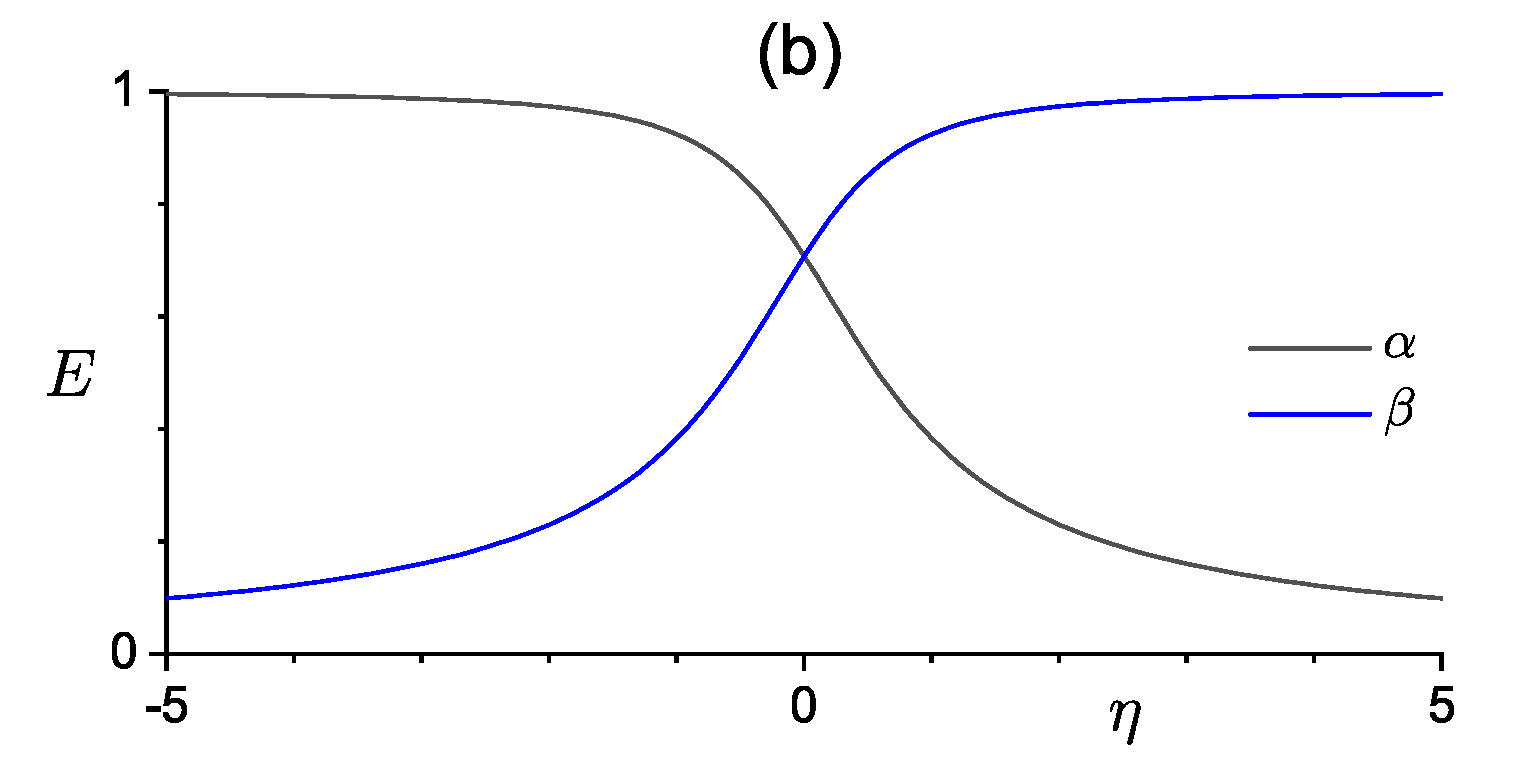
\epsfig{file=TwoLevelABEta.eps,width=\linewidth}
        \end{subfigure}
    	\scaption{
			Dynamika komponent vlastních vektorů pro dvouhladinový systém (a) s proměnnou mimodiagonální interakcí [rovnice~\eqref{eq:TwoLevelXi}], (b) s proměnnou vzdáleností neporušených hladin na diagonále [rovnice~\eqref{eq:TwoLevelEta}].
		}
        \label{fig:TwoLevelAB}
	\end{figure}				

	\begin{figure}[!htbp]
        \begin{subfigure}{0.49\linewidth}
            \centering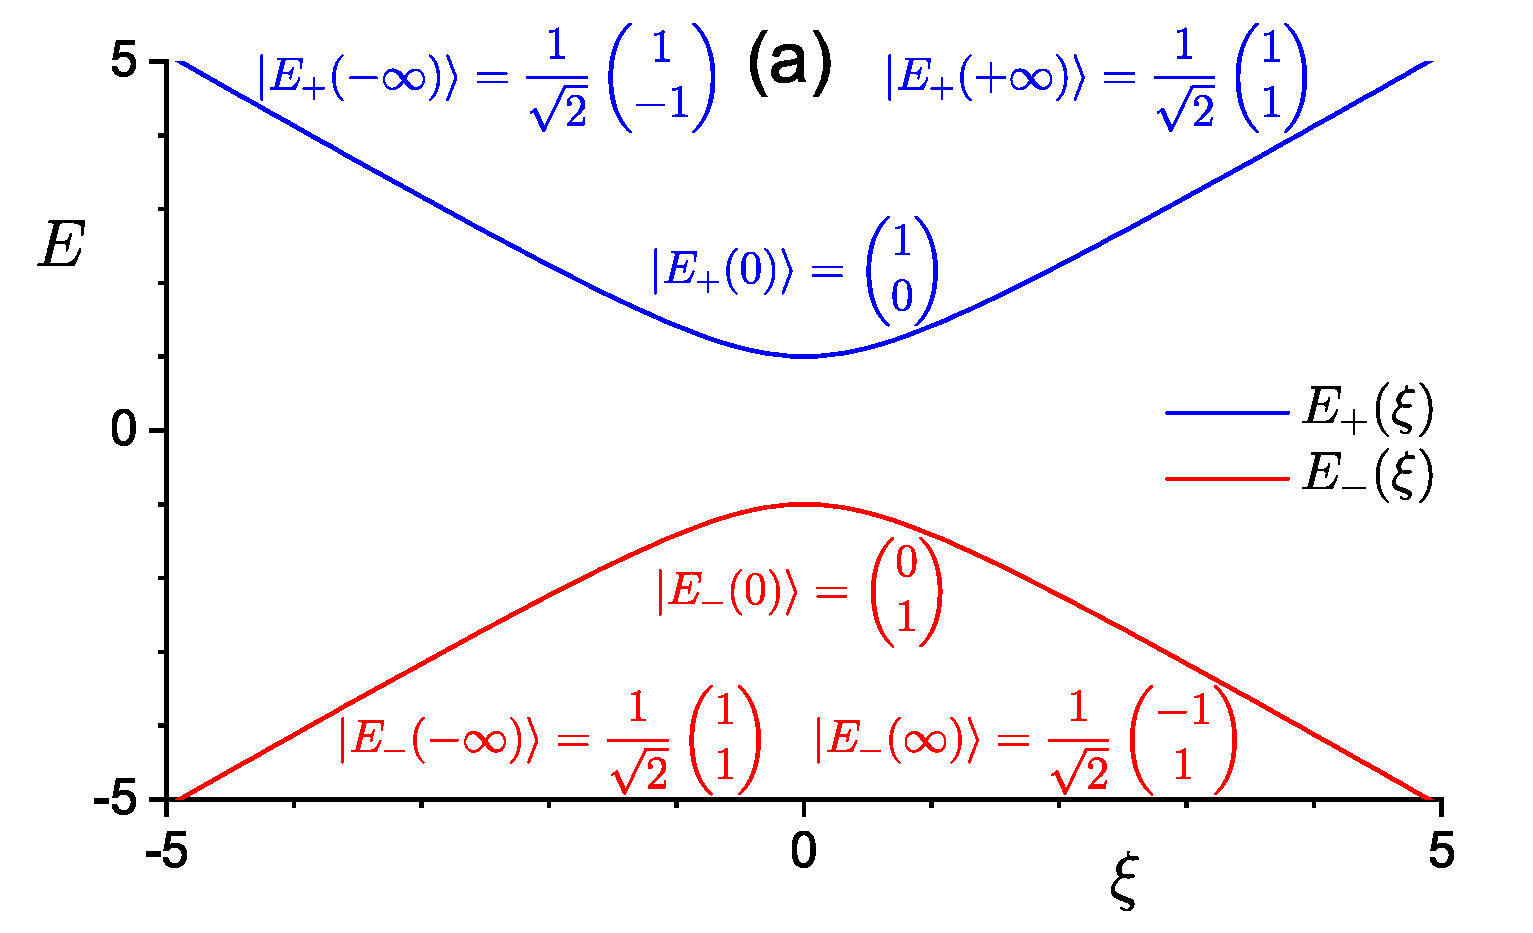
\epsfig{file=TwoLevelXi.eps,width=\linewidth}
        \end{subfigure}
        \hfill
        \begin{subfigure}{0.49\linewidth}
            \centering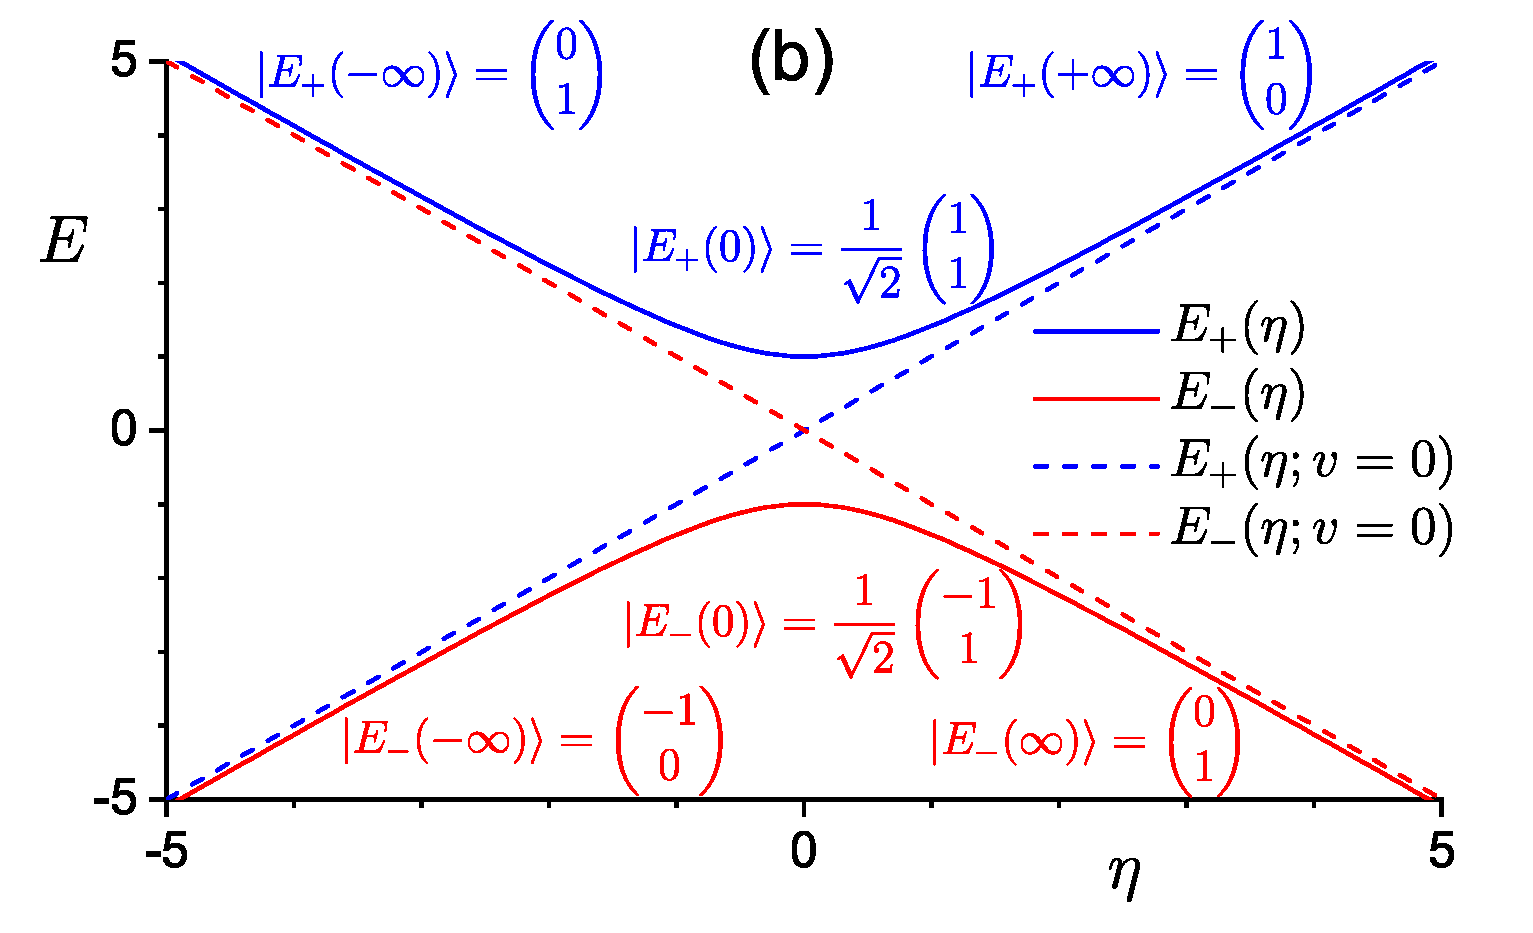
\epsfig{file=TwoLevelEta.eps,width=\linewidth}
        \end{subfigure}
		\scaption{
			Dynamika hladin pro dvouhladinový systém (a) s proměnnou mimodiagonální interakcí, (b) s proměnnou vzdáleností neporušených hladin na diagonále.
		}
    \label{fig:TwoLevelLD}
	\end{figure}				
\end{solution}

\subsection{Kvantový oblak}
\begin{enumerate}
\item
    Spočítejte vlastní hodnoty $E_{1,2,3}$ a vlastní vektory $\ket{E_{1,2,3}}$ systému popsaného Hamiltoniánem 
    \begin{equation}
        \matrix{H}
            =\matrix{H}_{0}+\matrix{V},\quad
        \mathrm{kde}\quad 
        \matrix{H}_{0}
            =\makematrix{e & 0 & 0 \\ 
                         0 & e & 0 \\ 
                         0 & 0 & e},\quad
        \matrix{V}
            =\makematrix{0 & v & v \\ 
                         v & 0 & v \\ 
                         v & v & 0}
    \end{equation}
    a načrtněte graf $E_{1,2,3}(v)$.
    
\item
    \emph{Zobecnění předchozího případu:}
    Určete vlastní hodnoty a normalizované ortogonální vlastní vektory Hamiltoniánu $\matrix{H}'$ obecné dimenze $N$,
    \begin{equation}
        \matrix{H}
            =\makematrix{e & v & v & v & \\ v & e & v & v & \\ v & v & e & v & \ldots 
                \\ v & v & v & e & \\ & & \vdots & & \ddots}.
    \end{equation}
    Tento Hamiltonián popisuje například částici na mřížce o $N$ pozicích, přičemž částice může přeskočit na libovolnou pozici mřížky a žádná pozice není upřednostněna.    
\end{enumerate}


\subsection{Kvantový řetízek}
Určete vlastní hodnoty a normalizované vlastní vektory Hamiltoniánu dimenze $N$ ve tvaru tridiagonální matice    
\begin{equation}
    \matrix{H}
        =\makematrix{e & v & 0 & 0 & \\ v & e & v & 0 & \\ 0 & v & e & v & \ldots 
            \\ 0 & 0 & v & e & \\ & & \vdots & & \ddots}.
\end{equation}
Jak se bude měnit energetické spektrum s rostoucím $N$?

\begin{note}[Nápověda:]
    V charakteristické rovnici identifikujte diferenční rovnici pro složky $c_{k}, k=1,\cdots,n$ vlastních vektorů a řešte ji pomocí násady $c_{k}=u^{k}$.
\end{note}

\begin{note}
    Tento Hamiltonián popisuje například částici na řetízku délky $N$, která smí \uv{přeskočit} jen na sousední pozice:
    \begin{equation}
        \operator{H}=e\sum_{k=1}^{N}\ket{k}\bra{k}+v\sum_{n=1}^{N-1}\left(\ket{k}\bra{k+1}+\ket{k+1}\bra{k}\right),
    \end{equation}
    kde $\left\{\ket{k},k=1,\dotsc,N\right\}$ je ortonormální báze.
    V případě, kdy $N$ je velké, se jedná o jednoduchý model jednorozměrného krystalu.\index{model!krystalu}
\end{note}


\np
\section{Vícečásticové systémy}

\subsection{Dvě částice se spinem \texorpdfstring{$\frac{1}{2}$}{1/2}}\index{moment hybnosti!skládání}\label{sec:TwoSpins}
Studovaný systém se skládá ze dvou rozlišitelných částic se spinem $\frac{1}{2}$.
Měřitelné veličině $A$ odpovídá operátor
\begin{equation}
    \operator{A}
        =\frac{\omega}{\hbar}\left(\operator{S}_{1}^{2}-\operator{S}_{2}^{2}\right),
\end{equation}	
kde $\operator{S}_{j}$ je $j$-tá složka operátoru celkového spinu\footnote{
    Obvykle se používá jednodušší zápis
    \begin{equation}
        \operator{S}_{j}=\frac{\hbar}{2}\left(\sigma_{j}^{(1)}+\sigma_{j}^{(2)}\right),
    \end{equation}
    kterému je však vždy potřeba rozumět ve smyslu rovnice~\eqref{eq:TwoSpins}.
    Viz též kapitola~\ref{sec:SkladaniMomentuHybnosti}.
}
\begin{equation}
    \operator{S}_{j}
        =\frac{\hbar}{2}\left[\matrix{\sigma}_{j}^{(1)}\otimes\matrix{1}^{(2)}+\matrix{1}^{(1)}\otimes\matrix{\sigma}_{j}^{(2)}\right]
    \label{eq:TwoSpins}
\end{equation}
a $\matrix{\sigma}_{j}$ jsou Pauliho matice.
Horní index v závorce značí, zda operátor působí na Hilbertově prostoru $\hilbert{H}^{(1)}$ první, resp. $\hilbert{H}^{(2)}$ druhé částice, dolní index udává složku v kartézském prostoru.

\begin{enumerate}
\item
    Nalezněte všechny hodnoty, které lze pozorovat při měření veličiny $A$.\index{měření}		

\item
    Jaká je pravděpodobnost nalezení jednotlivých hodnot a jaký bude stav systému po měření, pokud byl před měřením připraven ve stavu 
    \begin{equation}
        \ket{\psi}
            =\ket{x+}^{(1)}\otimes\ket{x+}^{(2)}\,\mathrm{?}
    \end{equation}		

\item    
    Ukažte, že stav
    \begin{equation}
        \ket{\psi'}
            =\frac{1}{\sqrt{2}}\left[\ket{x+}^{(1)}\otimes\ket{x-}^{(2)}-
                \ket{x-}^{(1)}\otimes\ket{x+}^{(2)}\right]
    \end{equation}
    je provázaný\index{entanglement} (nelze ho faktorizovat) a nalezněte pravděpodobnost naměření vlastních hodnot operátoru $\operator{A}$, je-li systém před měřením připraven v tomto stavu.
\end{enumerate}

\begin{solution}
	\begin{enumerate}
	\item
		První část úlohy vede na hledání spektra operátoru $\operator{A}$.
		V první řadě je potřeba vyjádřit si operátor celkového spinu $\vectoroperator{S}$.
        Jednotlivé jeho složky jsou dány maticemi\index{součin!direktní}
        \begin{subequations}
            \begin{align}
                \matrix{S}_{1}
                    &=\frac{\hbar}{2}
                        \left[\makematrix{0 & 1 \\ 1 & 0}\otimes\makematrix{1 & 0 \\ 0 & 1}+
                            \makematrix{1 & 0 \\ 0 & 1}\otimes\makematrix{0 & 1 \\ 1 & 0}\right]\nonumber\\
                    &=\frac{\hbar}{2}
                        \left[\makematrix{0\makematrix{1 & 0 \\ 0 & 1} & 1\makematrix{1 & 0 \\ 0 & 1}\\
                                        1\makematrix{1 & 0 \\ 0 & 1} & 0\makematrix{1 & 0 \\ 0 & 1}}
                            +\makematrix{1\makematrix{0 & 1 \\ 1 & 0} & 0\makematrix{0 & 1 \\ 1 & 0}\\
                                        0\makematrix{0 & 1 \\ 1 & 0} & 1\makematrix{0 & 1 \\ 1 & 0}}\right]\nonumber\\
                    &=\frac{\hbar}{2}
                        \left[\makematrix{0 & 0 & 1 & 0 \\ 0 & 0 & 0 & 1 \\ 1 & 0 & 0 & 0 \\ 0 & 1 & 0 & 0}
                            +\makematrix{0 & 1 & 0 & 0 \\ 1 & 0 & 0 & 0 \\ 0 & 0 & 0 & 1 \\ 0 & 0 & 1 & 0}
                            \right]\nonumber\\
                    &=\frac{\hbar}{2}\makematrix{0 & 1 & 1 & 0 \\ 1 & 0 & 0 & 1 \\ 1 & 0 & 0 & 1 \\ 0 & 1 & 1 & 0},\\
                \matrix{S}_{2}
                    &=\frac{\hbar}{2}\makematrix{0 & -\im & -\im & 0 \\ \im & 0 & 0 & -\im \\ \im & 0 & 0 & -\im \\ 0 & \im & \im & 0},\\
                \matrix{S}_{3}
                    &=\hbar\makematrix{1 & 0 & 0 & 0 \\ 0 & 0 & 0 & 0 \\ 0 & 0 & 0 & 0 \\ 0 & 0 & 0 & -1},
            \end{align}
        \end{subequations}
        jejich kvadráty jsou
		\begin{equation}
			\matrix{S}_{1}^{2}
				=\frac{\hbar^{2}}{2}\makematrix{1 & 0 & 0 & 1 \\ 0 & 1 & 1 & 0 \\ 0 & 1 & 1 & 0 \\ 1 & 0 & 0 & 1},
            \quad
			\matrix{S}_{2}^{2}
				=\frac{\hbar^{2}}{2}\makematrix{1 & 0 & 0 & -1 \\ 0 & 1 & 1 & 0 \\ 0 & 1 & 1 & 0 \\ -1 & 0 & 0 & 1},
            \quad
            \matrix{S}_{3}^{2}
				=\hbar^{2}\makematrix{1 & 0 & 0 & 0 \\ 0 & 0 & 0 & 0 \\ 0 & 0 & 0 & 0 \\ 0 & 0 & 0 & 1},
		\end{equation}
		a maticové vyjádření operátoru $\operator{A}$ má tudíž tvar
		\begin{equation}
			\matrix{A}=\hbar\omega\makematrix{0 & 0 & 0 & 1 \\ 0 & 0 & 0 & 0 \\ 0 & 0 & 0 & 0 \\ 1 & 0 & 0 & 0}.
		\end{equation}		
		Vlastní čísla $a$ této matice se určí diagonalizací
		\begin{equation}
			\det\left(\matrix{A}-a\matrix{1}\right)
				=\det\makematrix{-a & 0 & 0 & \hbar\omega \\ 0 & -a & 0 & 0 \\	0 & 0 & -a & 0 \\ \hbar\omega & 0 & 0 & -a}
				=a^{2}\left[a^{2}-\left(\hbar\omega\right)^{2}\right]=0.
		\end{equation}
		Operátor $\operator{A}$ má tedy tři různé vlastní hodnoty, přičemž jedna je dvojnásobně degenerovaná:\index{spektrum!degenerované}
		\begin{equation}
            a_{1,2}
                =0,\quad 
            a_{3}
                =\hbar\omega,\quad
            a_{4}
                =-\hbar\omega.
		\end{equation}
		Odpovídající vlastní vektory příslušející degenerované vlastní hodnotě $a_{1,2}=0$ musejí ležet v dvourozměrném charakteristickém podprostoru a musejí být ortonormální, jinak je lze zvolit libovolně, například\sfootnote{
			Jiná rovnocenná volba může být
			\begin{equation}
                \ket{a_{1}'}
                    =\frac{1}{\sqrt{2}}\makematrix{0 \\ 1 \\ 1 \\ 0},\quad
                \ket{a_{2}'}
                    =\frac{1}{\sqrt{2}}\makematrix{0 \\ 1 \\ -1 \\ 0}.
			\end{equation}
		}		
		\begin{equation}
            \ket{a_{1}}
                =\makematrix{0 \\ 1 \\ 0 \\ 0},\quad
            \ket{a_{2}}
                =\makematrix{0 \\ 0 \\ 1 \\ 0}.
		\end{equation}
		Normalizované vlastní vektory příslušející zbývajícím dvěma vlastním hodnotám jsou určeny (až na komplexní fázi) jednoznačně:
		\begin{equation}
            \ket{a_{3}}
                =\frac{1}{\sqrt{2}}\makematrix{1 \\ 0 \\ 0 \\ 1},\quad
            \ket{a_{4}}
                =\frac{1}{\sqrt{2}}\makematrix{1 \\ 0 \\ 0 \\ -1}.
        \end{equation}		
        
	\item
		Dvourozměrné Hilbertovy prostory jednotlivých spinů $\mathcal{H}^{(1)}$ a $\mathcal{H}^{(2)}$ jsou realizovány pomocí báze dané vlastními vektory třetí Pauliho matice, viz~\eqref{eq:SigmaXYZ}.
		Hilbertův prostor celého systému $\hilbert{H}=\hilbert{H}^{(1)}\otimes\hilbert{H}^{(2)}$ je čtyřrozměrný a za jeho bázi lze volit $\mathcal{B}=\left\{\ket{\uparrow\uparrow},\ket{\uparrow\downarrow},\ket{\downarrow\uparrow},\ket{\downarrow\downarrow}\right\}$.\sfootnote{
			Jedná se o zjednodušený zápis $\ket{\uparrow\uparrow}\equiv\ket{\uparrow}^{(1)}\otimes\ket{\uparrow}^{(2)}$ a analogicky u zbylých tří vektorů.
			Vektory báze mají sloupcové vyjádření
			\begin{equation}
                \ket{\uparrow\uparrow}
                    =\makematrix{1 \\ 0}\otimes\makematrix{1 \\ 0}=\makematrix{1 \\ 0 \\ 0 \\ 0},\quad
                \ket{\uparrow\downarrow}
                    =\makematrix{0 \\ 1 \\ 0 \\ 0},\quad
                \ket{\downarrow\uparrow}
                    =\makematrix{0 \\ 0 \\ 1 \\ 0},\quad
                \ket{\downarrow\downarrow}
                    =\makematrix{0 \\ 0 \\ 0 \\ 1}.
                \label{eq:TwoSpinsBasis}
			\end{equation}
			To znamená, že vektor $\ket{\uparrow\uparrow}$ odpovídá situaci, kdy oba spiny míří ve směru osy $z$,
			vektor $\ket{\uparrow\downarrow}$ popisuje stav, kdy první spin míří ve směru osy $z$, 
			zatímco druhý proti, atd.
		}
		V ní se vektor $\ket{\psi}$ vyjádří jako
		\begin{equation}
			\ket{\psi}
				=\frac{1}{\sqrt{2}}\makematrix{1 \\ 1}\otimes\frac{1}{\sqrt{2}}\makematrix{1 \\ 1}
				=\frac{1}{2}\makematrix{1 \\ 1 \\ 1 \\ 1}.
		\end{equation}		
        Pravděpodobnosti naměření jednotlivých hodnot pozorovatelné veličiny $A$ pak vycházejí
        \begin{subequations}
            \begin{align}
                p_{a_{1,2}}
                    &=\abs{\braket{\phi_{1}}{\psi}}^{2}+\abs{\braket{\phi_{2}}{\psi}}^{2}
                    =\frac{1}{4}+\frac{1}{4}=\frac{1}{2},\\
                p_{a_{3}}
                    &=\abs{\braket{\phi_{3}}{\psi}}^{2}=\frac{1}{2},\\
                p_{a_{4}}
                    &=\abs{\braket{\phi_{4}}{\psi}}^{2}=0.
            \end{align}
        \end{subequations}
        Kontrolou je, že celková pravděpodobnost se sečte na $1$, což znamená, že s jistotou naměříme aspoň jednu z uvedených vlastních hodnot.
		
		Stav systému po naměření hodnot $a_{3}$, resp. $a_{4}$ bude dán vlastními vektory $\ket{a_{3}}$, resp. $\ket{a_{4}}$.
        Po naměření dvojnásobně degenerované vlastní hodnoty $a_{1,2}$ bude systém ve stavu daném libovolnou lineární kombinací vektorů $\ket{a_{1}}$ a $\ket{a_{2}}$.		
        
	\item
		Vektor $\ket{\psi'}$ vyjádřený v bázi $\mathcal{B}$~\eqref{eq:TwoSpinsBasis} je
		\begin{align}
			\ket{\psi'}
				&=\frac{1}{\sqrt{2}}\left[
					\frac{1}{\sqrt{2}}\makematrix{1 \\ 1}\otimes\frac{1}{\sqrt{2}}\makematrix{1 \\ -1}
					-\frac{1}{\sqrt{2}}\makematrix{1 \\ -1}\otimes\frac{1}{\sqrt{2}}\makematrix{1 \\ 1}\right]\nonumber\\
				&=\frac{1}{\sqrt{2}}\left[\frac{1}{2}\makematrix{1 \\ -1 \\ 1 \\ -1}-\frac{1}{2}\makematrix{1 \\ 1 \\ -1 \\ -1}\right]
				 =\frac{1}{\sqrt{2}}\makematrix{0 \\ -1 \\ 1 \\ 0}.
        \end{align}
        Faktorizovatelný vektor systému složeného ze dvou dvourozměrných podsystémů musí být obecně možné zapsat jako
        \begin{align}
            \ket{\psi'}
                &=\ket{\phi_{1}}^{(1)}\otimes\ket{\phi_{2}}^{(2)}\nonumber\\
                &=\left(\alpha\ket{\uparrow}^{(1)}+\beta\ket{\downarrow}^{(1)}\right)\otimes\left(\gamma\ket{\uparrow}^{(2)}+\delta\ket{\uparrow}^{(2)}\right)\nonumber\\
                &=\alpha\gamma\ket{\uparrow\uparrow}+\alpha\delta\ket{\uparrow\downarrow}+\beta\gamma\ket{\downarrow\uparrow}+\beta\delta\ket{\downarrow\downarrow}\nonumber\\
                &=a\ket{\uparrow\uparrow}+b\ket{\uparrow\downarrow}+c\ket{\downarrow\uparrow}+d\ket{\downarrow\downarrow},
        \end{align}
        kde $\alpha,\beta,\gamma,\delta$, resp. $a,b,c,d$ jsou komplexní čísla.
        Z posledních dvou řádků vyplývá podmínka faktorizovatelnosti stavu:
        \begin{equation}
            \important{ad-bc=0.}
            \label{eq:TwoSpinFactorize}
        \end{equation}
        V případě stavu $\ket{\psi'}$ je $a=0$, $b=-1/\sqrt{2}$, $c=1/\sqrt{2}$, $d=0$ a podmínka~\eqref{eq:TwoSpinFactorize} splněna není.
        Stav je tedy provázaný (entanglovaný).

		Pravděpodobnosti naměření jednotlivých vlastních hodnot operátoru $\operator{A}$, je-li systém ve stavu $\ket{\psi'}$, jsou
		\begin{equation}
            p_{a_{1,2}}
                =1,\quad
            p_{a_{3}}
                =p_{a_{4}}
                =0.
		\end{equation}		
	\end{enumerate}
\end{solution}

\subsection{Trojhladinový systém}
    Uvažujte jednoduchý trojhladinový systém, kde index hladiny je $h=1,2,3$, první hladina má energii $d$ a vzdálenost mezi sousedními hladinami je také $d$ (jednočásticové spektrum je ekvidistantní).
    Na každé hladině se můžou nacházet nanejvýš dvě částice (každá hladina je dvojnásobně degenerovaná).
    Jednočásticové stavové vektory jsou $\ket{h\sigma}$, kde $\sigma=\pm$.

	\begin{figure}[!htbp]
        \centering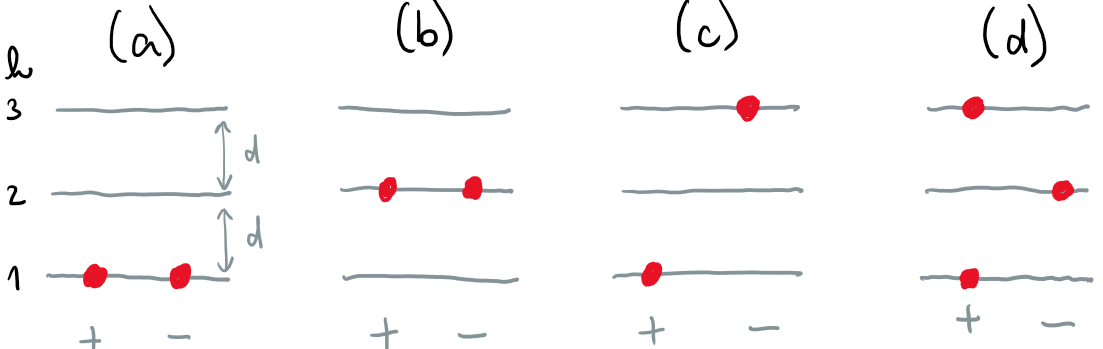
\epsfig{file=3levels.png,width=0.7\linewidth}
		\caption{
			Příklady několika možných vícečásticových konfigurací v trojhladinovém systému.
		}
    \label{fig:ThreeLevel}
	\end{figure}				

    \begin{enumerate}
        \item Kolik odlišných dvoučásticových stavových vektorů (Slaterových determinantů) lze zkonstruovat? 
        
        \item Předpokládejte, že v systému jsou pouze dvě částice, které se mohou nacházet výhradně v páru na jedné z nejnižších dvou hladin $h=1$ a $h=2$ [obrázek~\ref{fig:ThreeLevel}~(a)--(b)] a že jeho Hamiltonián má tvar
        \begin{equation}
            \operator{H}=\operator{H}_{0}+\operator{H}_{\mathrm{I}},
        \end{equation}
        přičemž jednočásticová část Hamiltoniánu splňuje
        \begin{equation}
            \operator{h}_{0}\ket{h\sigma}=hd\ket{h\sigma}.
        \end{equation}
        Dvoučásticové maticové elementy Hamiltoniánu $\operator{H}_{\mathrm{I}}$ mají všechny stejnou hodnotu $g$.
        Jak vypadá matice Hamiltoniánu $\operator{H}$?

        \item
            Jaké jsou vlastní hodnoty a vlastní vektory matice $\matrix{H}$?

        \item
            Jaký je překryv stavu odpovídajícího nižšímu vlastnímu stavu Hamiltoniánu $\operator{H}$ s dvoučásticovým stavem popisujícím dvě částice na hladině $p=2$?\footnote{
                Někdy se také říká, že se jedná o \emph{příměs} stavu $\ket{\psi_{2}}$ k základnímu stavu.
            }
            
        \item
            Přidejte nyní třetí hladinu, přičemž předpokládejte stále, že se částice mohou nacházet pouze v párech.
    \end{enumerate}

    \begin{solution}
        \begin{enumerate}
            \item Počty vícečásticových stavů lze určit obecně pro systém $n$ částic s $H$ hladinami.
                Celkový počet pozic, na které můžeme částice umístit, je $P=2H$ (počet hladin krát počet částic, které lze umístit na jednu hladinu).
                Počet $n$-částicových funkcí je pak dán počtem všech možných kombinací $n$ částic na $P$ pozicích, tj.
                \begin{equation}
                    N=\makematrix{2H \\ n}.
                \end{equation}

                Konkrétně pro $H=3$ a $n=2$ vychází
                \begin{equation}
                    N=15.
                \end{equation}
                Všechny 15 možných konfigurací je znázorněno na obrázku~\ref{fig:ThreeLevelTwoParticles}.

                \begin{figure}[!htbp]
                    \centering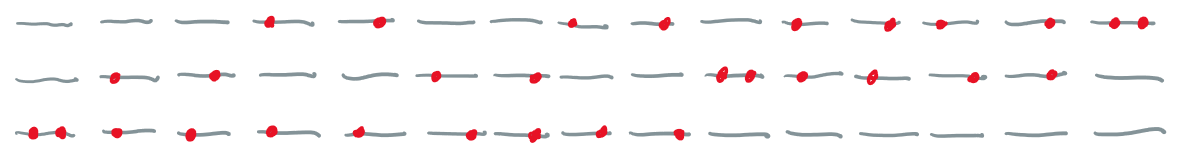
\epsfig{file=3levels2particles.png,width=0.9\linewidth}
                    \scaption{
                        Všechny možné dvoučásticové konfigurace v tříhladinovém systému.
                    }
                    \label{fig:ThreeLevelTwoParticles}
                \end{figure}				
            
            \item
                Podprostor uvažovaných dvoučásticových stavů ($n=2$) je dvourozměrný a stavy jsou dány Slaterovými determinanty\sfootnote{
                    Zkrácený zápis je nutné číst jako
                    \begin{equation}
                        \ket{1+}\ket{1-}\equiv\ket{1+}^{(1)}\otimes\ket{1-}^{(2)},
                    \end{equation}
                    tj. první ket odpovídá první částici, druhý ket druhé částici.
                }
                \begin{equation}
                    \label{eq:ThreeLevelTwoPairs}
                    \ket{\psi_{j}}=\frac{1}{\sqrt{n!}}\det{\makematrix{\ket{j+} & \ket{j+} \\ \ket{j-} & \ket{j-}}}\Rightarrow
                    \begin{cases}
                        \ket{\psi_{1}}=\frac{1}{\sqrt{2}}\left(\ket{1+}\ket{1-}-\ket{1-}\ket{1+}\right),\\
                        \ket{\psi_{2}}=\frac{1}{\sqrt{2}}\left(\ket{2+}\ket{2-}-\ket{2-}\ket{2+}\right).
                    \end{cases}
                \end{equation}
                Tyto stavy jsou normalizované a na sebe kolmé.

                Dvoučásticový volný Hamiltonián je
                \begin{equation}
                    \operator{H}_{0}=\operator{h}_{0}^{(1)}+\operator{h}_{0}^{(2)}=\operator{h}_{0}\otimes\operator{1}+\operator{1}\otimes\operator{h}_{0}
                \end{equation}
                a pro jeho maticové elementy v bázi dané vektory~\eqref{eq:ThreeLevelTwoPairs} platí
                \begin{align}
                    \matrixelement{\psi_{j}}{\operator{H}_{0}}{\psi_{k}}
                        &=\frac{1}{2}\left(\bra{j+}\bra{j-}-\bra{j-}\bra{j+}\right)\operator{H}_{0}\left(\ket{k+}\ket{k-}-\ket{k-}\ket{k+}\right)\nonumber\\
                        &=\frac{1}{2}\bigg(\underbrace{\matrixelement{j+}{\operator{h}_{0}}{k+}}_{jd\delta_{jk}}\underbrace{\braket{j-}{k-}}_{\delta_{jk}}
                            +\underbrace{\braket{j+}{k+}}_{\delta_{jk}}\underbrace{\matrixelement{j-}{\operator{h}_{0}}{k-}}_{jd\delta_{jk}}\nonumber\\
                        &\quad\ \ \underbrace{-\matrixelement{j+}{\operator{h}_{0}}{k-}}_{0}\underbrace{\braket{j-}{k+}}_{0}
                            -\underbrace{\braket{j+}{k-}}_{0\dotsb}\matrixelement{j-}{\operator{h}_{0}}{k+}\nonumber\\
                        &\quad\ \ -\matrixelement{j-}{\operator{h}_{0}}{k+}\braket{j+}{k-}
                            -\braket{j-}{k+}\matrixelement{j+}{\operator{h}_{0}}{k-}\nonumber\\
                        &\quad\ \ +\matrixelement{j-}{\operator{h}_{0}}{k-}\braket{j+}{k+}
                            +\braket{j-}{k-}\matrixelement{j+}{\operator{h}_{0}}{k+}\bigg)\nonumber\\
                        &=\frac{1}{2}\left(jd+jd+jd+jd\right)\delta_{jk}=2jd\delta_{jk},
                \end{align}
                což v maticové realizaci dá
                \begin{equation}
                    \matrix{H}_{0}=\makematrix{2d & 0 \\ 0 & 4d}.
                \end{equation}
                Matice interakčního Hamiltoniánu má tvar
                \begin{equation}
                    \matrix{H}_{\mathrm{I}}=\makematrix{g & g \\ g & g},
                \end{equation}
                takže celkový Hamiltonián je
                \begin{equation}
                    \label{eq:ThreeLevelH}
                    \matrix{H}=\makematrix{2d + g & g \\ g & 4d + g}.
                \end{equation}

            \item
                Matici~\eqref{eq:ThreeLevelH} lze přepsat na tvar
                \begin{equation}
                    \matrix{H}=\left(3d+g\right)\matrix{1}-d\sigma_{3}+g\sigma_{1},
                \end{equation}
                čož odpovídá Hamiltoniánu detailně propočteném v příkladu~\ref{sec:AvoidedCrossing}, kde se přiřadí $d\leftrightarrow e,g\leftrightarrow\nu$, výsledné spektrum se posune v energii o $3d+g$ a prohodí se vlastní vektory.
                Vlastní hodnoty jsou tedy
                \begin{equation}
                    E_{\pm}=3d+g\pm\sqrt{d^{2}+g^{2}}
                \end{equation}
                a odpovídající vlastní vektory
                \begin{subequations}
                    \begin{align}
                        \ket{\phi_{-}}&=\alpha\ket{\psi_{2}}+\beta\ket{\psi_{1}},\\
                        \ket{\phi_{+}}&=\beta\ket{\psi_{2}}-\alpha\ket{\psi_{1}},
                    \end{align}                        
                \end{subequations}
                kde koeficienty $\alpha$ a $\beta$ jsou dány vztahy~\eqref{eq:TwoLevelEV}.
                Vektory $\ket{\phi_{\pm}}$ jsou jen lineární kombinací vektorů antisymetrických vůči záměně částic, samy jsou tedy antisymetrické při záměně $\ket{j\sigma}^{(1)}\leftrightarrow\ket{j\sigma}^{(2)}$.

            \item
                Překryv je dán amplitudou pravděpodobnosti
                \begin{equation}
                    \braket{\psi_{2}}{\phi_{-}}=\alpha=\frac{g}{\sqrt{g^{2}+\left(d+\sqrt{g^{2}+d^{2}}\right)}}\sim\frac{1}{2}\frac{g}{e},
                \end{equation}
                kde poslední rovnost platí pro $g\ll e$.

            \item
                Rozšíření systému o třetí hladinu vede na matici Hamiltoniánu
                \begin{equation}
                    \matrix{H}'=\makematrix{2d + g & g & g \\ g & 4d + g & g \\ g & g & 6d + g},
                \end{equation}
                kterou je nutné řešit numericky pro konkrétní hodnoty parametrů $d,g$.
            \end{enumerate}
    \end{solution}

    \begin{note}
        Dodatečné kvantové číslo jednočásticových stavů označené $\sigma$ lze identifikovat s projekcí spinu částice.
        Pak je možné rozdělit Hilbertův prostor jednočásticových stavů jako $\hilbert{H}_{1}=\hilbert{H}_{1\mathrm{h}}\otimes\hilbert{H}_{1\mathrm{p}}$, kde první odpovídá umístění částice na jednu z hladin a druhý pak jejímu spinu.

        Dvoučásticový Hilbertův prostor lze pak rozdělit na
        \begin{equation}
            \hilbert{H}_{2}=\left(\hilbert{H}_{2\mathrm{h}}^{\mathrm{S}}\otimes\hilbert{H}_{2\mathrm{s}}^{\mathrm{S}}\right)\oplus\left(\hilbert{H}_{2\mathrm{h}}^{\mathrm{A}}\otimes\hilbert{H}_{2\mathrm{s}}^{\mathrm{T}}\right),
        \end{equation}
        kde $\hilbert{H}_{2\mathrm{h}}^{S,A}$ je symetrická, resp. antisymetrická kombinace hladinových stavů a $\hilbert{H}_{2\mathrm{s}}^{S,T}$ je singletní, resp. tripletní spinový stav.
        Stavy~\eqref{eq:ThreeLevelTwoPairs} pak mají symetrickou hladinovou a singletní (antisymetrickou) spinovou část,
        \begin{equation}
            \ket{\psi_{j}}=\ket{jj}\otimes\ket{00},
        \end{equation}
        kde
        \begin{subequations}            
            \begin{equation}
                \ket{jj}=\ket{j}^{(1)}\otimes\ket{j}^{(2)}
            \end{equation}
            je hladinová část a
            \begin{equation}
                \ket{00}=\frac{1}{\sqrt{2}}\left(\ket{+}^{(1)}\otimes\ket{-}^{(2)}-\ket{-}^{(1)}\otimes\ket{+}^{(2)}\right)
            \end{equation}
            je singletní spinový stav.
        \end{subequations}
    \end{note}

    \begin{note}
        Se singletními a tripletními spinovými stavy se také počítá v příkladech~\ref{sec:Mionium}, \ref{sec:VanDerWaals} a~\ref{sec:GaussovskaPoruchaFermiony}.
    \end{note}
\np

\section{Harmonický oscilátor}\label{sec:HO}
\subsection[Vlastnosti posunovacích operátorů]{Spektrum operátoru $\operator{n}=\operatorconjugate{a}\operator{a}$}\index{operátor!počtu}\label{sec:ShiftOperators}
Je zadán operátor $\operator{a}$ a operátor $\operatorconjugate{a}$ k němu sdružený, které mezi sebou splňují komutační relace\footnote{
    Vztahu~\eqref{eq:ShiftOperatorCommutator} je třeba rozumět ve smyslu $\commutator{\operator{a}}{\conjugate{\operator{a}}}=\operator{1}$, kde $\operator{1}$ je operátor identity, podobně jako je tomu například u komutačních relací samosdružených operátorů souřadnice a hybnosti $\commutator{\operator{x}}{\operator{p}}=\im\hbar\operator{1}$, které se běžně zkráceně zapisují $\commutator{\operator{x}}{\operator{p}}=\im\hbar$.
}\footnote{
    Obecněji lze uvažovat komutační relace
    \begin{equation}
        \commutator{\operator{A}}{\conjugate{\operator{A}}}
            =m,\qquad 
        m\in\mathbb{R}^{+}.
    \end{equation}
    Ty přejdou na~\eqref{eq:ShiftOperatorCommutator} přeškálováním $\operator{a}=\operator{A}/\sqrt{m}$.		
}
\begin{equation}
    \commutator{\operator{a}}{\conjugate{\operator{a}}}
        =1.
    \label{eq:ShiftOperatorCommutator}
\end{equation}
Definujme operátor 
\begin{equation}
    \operator{n}
        \equiv\conjugate{\operator{a}}\operator{a}.
    \label{eq:NumberOperator}
\end{equation}

\begin{enumerate}
\item 
    Ukažte, že operátor $\operator{n}$ je samosdružený a pozitivně definitní.

\item
    Nalezněte, čemu se rovnají komutátory $\commutator{\operator{n}}{\operator{a}^{k}}$ a $\commutator{\operator{n}}{\left(\conjugate{\operator{a}}\right)^{k}}$ pro $k\in{\mathbb N}$.

\item
    Ukažte, čemu se rovná $\conjugate{\operator{a}}\ket{n}$, $\operator{a}\ket{n}$, kde $\ket{n}$ je vlastní vektor operátoru $\operator{n}$ příslušející vlastní hodnotě $n$.

\item
    Nalezněte všechny vlastní hodnoty $n$ operátoru $\operator{n}$.
    
\item 
    Nalezněte normalizované vlastní vektory operátoru $\operator{n}$.
    
\item 
    Nalezněte tvar operátorů $\operator{a}$ a $\conjugate{\operator{a}}$ v maticové realizaci.
\end{enumerate}

\begin{solution}
	\begin{enumerate}	
	\item 
		Samosdruženost plyne z identit\index{operátor!samosdružený}
		\begin{equation}
			\operatorconjugate{n}
				=\conjugate{\left(\operatorconjugate{a}\operator{a}\right)}
				=\conjugate{\operator{a}}\conjugate{\left(\operatorconjugate{a}\right)}
				=\operatorconjugate{a}\operator{a}=\operator{n}.
		\end{equation}
        \trick{Díky samosdruženosti existuje spektrální rozklad} operátoru $\operator{n}$,
		\begin{equation}
            \operator{n}\ket{n}=n\ket{n},
            \label{eq:NumberOperatorSpectrum}
		\end{equation}
        kde $n$ je reálné číslo a $\ket{n}$ odpovídající normalizovaný vlastní vektor, $\braket{n}{n}=1$.
        
        Pozitivita operátoru $\operator{n}$ znamená, že všechny jeho vlastní hodnoty jsou nezáporné.\index{operátor!pozitivně definitní}
		Platí
		\begin{equation}
			\matrixelement{n}{\operator{n}}{n}
				=n\braket{n}{n}
				=n
		\end{equation}
		a zároveň
		\begin{equation}
			\matrixelement{n}{\operator{n}}{n}
				=\matrixelement{n}{\conjugate{\operator{a}}\operator{a}}{n}
				=\abss{\operator{a}\ket{n}}
				\geq0,
		\end{equation}
		takže opravdu
		\begin{equation}
			n\geq0.
		\end{equation}
	
	\item
		Pro $k=1$ je
		\begin{equation}
			\commutator{\operator{n}}{\operator{a}}
				=\commutator{\conjugate{\operator{a}}\operator{a}}{\operator{a}}
				=\conjugate{\operator{a}}\underbrace{\commutator{\operator{a}}{\operator{a}}}_{0}
					+\underbrace{\commutator{\conjugate{\operator{a}}}{\operator{a}}}_{-1}\operator{a}
				=-\operator{a},
			\label{eq:NACommutator}
		\end{equation}
		kde druhá rovnost platí díky rozvoji komutátoru~\eqref{eq:CommutatorAB,C} a poslední rovnost vyplývá ze vztahu~\eqref{eq:ShiftOperatorCommutator}.
		Induktivní opakování tohoto postupu vede na
		\begin{align}
			\commutator{\operator{n}}{\operator{a}^{k}}
				&=\commutator{\operator{n}}{\operator{a}^{k-1}\operator{a}}
				 =\operator{a}^{k-1}\underbrace{\commutator{\operator{n}}{\operator{a}}}_{-\operator{a}}
					+\commutator{\operator{n}}{\operator{a}^{k-1}}\operator{a}\nonumber\\
				&=-\operator{a}^{k}+\commutator{\operator{n}}{\operator{a}^{k-2}\operator{a}}\operator{a}
				 =-\operator{a}^{k}+\operator{a}^{k-2}\underbrace{\commutator{\operator{n}}{\operator{a}}}_{-\operator{a}}\operator{a}
					+\commutator{\operator{n}}{\operator{a}^{k-2}}\operator{a}^{2}\nonumber\\
				&=-2\operator{a}^{k}+\commutator{\operator{n}}{\operator{a}^{k-3}\operator{a}}\operator{a}^{2}=\dotsb=-k\operator{a}^{k}.
		\end{align}
		Zcela analogicky se ukáže, že
		\begin{equation}
            \commutator{\operator{n}}{\left(\conjugate{\operator{a}}\right)^{k}}
                =k\left(\conjugate{\operator{a}}\right)^{k}.
		\end{equation}
	
	\item
        Vlastní hodnoty a vlastní vektory operátoru $\operator{n}$ splňují rovnici~\eqref{eq:NumberOperatorSpectrum}, kde $n\geq0$.
        Za předpokladu $n\neq0$ a díky vztahu~\eqref{eq:NACommutator} platí
		\begin{equation}
            \operator{n}\operator{a}\ket{n}
                =\left(\operator{a}\operator{n}-\operator{a}\operator{n}+\operator{n}{\operator{a}}\right)\ket{n}
				=\left(\operator{a}\operator{n}+\commutator{\operator{n}}{\operator{a}}\right)\ket{n}
				=\left(\operator{a}\operator{n}-\operator{a}\right)\ket{n}
				=\left(n-1\right)\operator{a}\ket{n}.
		\end{equation}
        Analogicky pak
		\begin{equation}
            \operator{n}\conjugate{\operator{a}}\ket{n}
                =\left(n+1\right)\conjugate{\operator{a}}\ket{n}.
		\end{equation}
		Vektory $\operator{a}\ket{n}$ a $\conjugate{\operator{a}}\ket{n}$ jsou tedy oba vlastními stavy operátoru 
		$\operator{n}$ příslušejícími vlastním hodnotám $n-1$, respektive $n+1$.
		Norma těchto vektorů je
        \begin{subequations}
            \begin{align}
                \abs{\matrixelement{n}{\conjugate{\operator{a}}\operator{a}}{n}}
                    &=\abs{\matrixelement{n}{\operator{n}}{n}}=n\abs{\braket{n}{n}}=n,\\
                \abs{\matrixelement{n}{\operator{a}\conjugate{\operator{a}}}{n}}
                    &=\abs{\matrixelement{n}{\conjugate{\operator{a}}\operator{a}+1}{n}}=n+1.
            \end{align}                
        \end{subequations}
        Normované vlastní vektory operátoru $\operator{n}$ jsou tedy navzájem svázány operátory $\operator{a}$ a $\conjugate{\operator{a}}$:
        \begin{subequations}
            \begin{empheq}[box=\fbox]{align}
                \ket{n-1}&\equiv\frac{1}{\sqrt{n}}\,\operator{a}\ket{n},\\
                \ket{n+1}&\equiv\frac{1}{\sqrt{n+1}}\,\conjugate{\operator{a}}\ket{n}.
            \end{empheq}
            \label{eq:AN}
        \end{subequations}
        
	\item
		$k$-násobným opakovaným působení operátoru $\operator{a}$ na stav $\ket{n}$ se dospěje k normovanému vektoru
		\begin{equation}
			\ket{n-k}\equiv\frac{1}{\sqrt{n(n-1)\dotsb(n-k)}}\,\operator{a}^{k}\ket{n},
		\end{equation}
		což je vlastní vektor operátoru $\operator{n}$ příslušející vlastní hodnotě $n-k$.
        \trick{Pozitivita operátoru však omezuje hodnoty $k$: Pro žádné $k$ není povoleno získat vektor, který by měl odpovídat záporné vlastní hodnotě.}
        Jelikož $k$ lze volit libovolně, musí spektrum operátoru bezpodmínečně obsahovat hodnotu $0$, tj. musí existovat vektor $\ket{0}$ takový, že
		\begin{equation}
			\operator{n}\ket{0}=0\ket{0}=0,
        \end{equation}        
        a tedy $\operator{a}\ket{0}=0$.       
        Další aplikace operátoru $\operator{a}$ dají identicky nulu.

		Spektrum operátoru $\operator{n}$ tedy tvoří všechna nezáporná celá čísla $n\in\mathbb{N}_{0}$.
		
	\item
		Všechny normalizované vlastní vektory $\ket{n}$ lze nagenerovat ze stavu $\ket{0}$ pomocí vícenásobného použití operátoru $\conjugate{\operator{a}}$ podle~\eqref{eq:AN}:
		\begin{equation}
			\important{
				\ket{n}=\frac{\left(\conjugate{\operator{a}}\right)^{n}}{\sqrt{n!}}\ket{0}.			
			}
			\label{eq:EigenstateNumberOperator}
		\end{equation}		
        
    \item
        Dimenze Hilbertova prostoru, na kterém působí operátory $\operator{a}$ a $\conjugate{\operator{a}}$, je nekonečná, přičemž za jeho bázi lze zvolit vektory $\ket{n}$. 
        V maticové realizaci lze tento vektor vyjádřit jako nekonečný sloupec
        \begin{equation}
            \ket{n}\equiv
            \begin{blockarray}{cc}  
                \begin{block}{(c)c}
                    0 & \\ 
                    \Vdots & \\ 
                    0 & \\ 
                    1 & \dotsb\ n\text{-tá pozice}\\ 
                    0 & \\ 
                    \Vdots & \\
                \end{block}
            \end{blockarray}                        
        \end{equation}
        Z algebraického vztahu mezi bázovými vektory~\eqref{eq:AN} vyplývá
        \begin{align}
            \label{eq:ANMatrix}
            \matrix{a}&=\makematrix{
                    0 & 1 & 0 & 0 & 0 & \\
                    0 & 0 & \sqrt{2} & 0 & 0 & \\
                    0 & 0 & 0 & \sqrt{3} & 0 & \dotsb \\ 
                    0 & 0 & 0 & 0 & \sqrt{4} & \\ 
                    0 & 0 & 0 & 0 & 0 & \\
                      &   &   & \vdots & & \ddots }, &
            \conjugate{\matrix{a}}&=\makematrix{
                    0 & 0 & 0 & 0 & 0 & \\
                    1 & 0 & 0 & 0 & 0 & \\
                    0 & \sqrt{2} & 0 & 0 & 0 & \dotsb \\ 
                    0 & 0 & \sqrt{3} & 0 & 0 & \\ 
                    0 & 0 & 0 & \sqrt{4} & 0 & \\
                    &   &   & \vdots & & \ddots }\equiv\transpose{\matrix{a}}.
        \end{align}
        Operátor $\operator{n}$ je v této bázi diagonální a jeho maticové vyjádření je
        \begin{equation}
            \matrix{n}=\makematrix{
                    0 & 0 & 0 & 0 & 0 & \\
                    0 & 1 & 0 & 0 & 0 & \\
                    0 & 0 & 2 & 0 & 0 & \dotsb \\
                    0 & 0 & 0 & 3 & 0 & \\
                    0 & 0 & 0 & 0 & 4 & \\
                    &   &   & \vdots & & \ddots }.
        \end{equation}
        K tomuto vztahu lze rovněž dospět pronásobením nekonečných matic~\eqref{eq:ANMatrix}, tj. $\matrix{n}=\conjugate{\matrix{a}}\matrix{a}$.
    \end{enumerate}
\end{solution}

\begin{note}
    Operátory $\operator{a}$, $\conjugate{\operator{a}}$ posouvají vlastní stav operátoru $\operator{n}$
    z vyšší vlastní hodnoty na nižší a naopak, proto se obvykle nazývají \emph{posunovací operátory}\index{operátor!posunovací}.
    Při využití těchto operátorů nad Fokovými prostory (kapitola~\ref{sec:ManyBody}), kde vytvářejí a ruší částice daných vlastností, se nazývají \emph{anihilační a kreační operátory}.
\end{note}

\subsection{Jednorozměrný harmonický oscilátor}\label{sec:HarmonicOscillator}\index{harmonický oscilátor}
Harmonický oscilátor je popsán Hamiltoniánem
\begin{equation}
    \important{
        \operator{H}
            =\frac{1}{2M}\operator{p}^{2}+\frac{1}{2}M\Omega^{2}\operator{x}^{2},
    }
    \label{eq:HOHamiltonianXY}
\end{equation}
kde $M$ je hmotnost kmitající částice, $\Omega=\sqrt{k/M}$ je úhlová frekvence oscilátoru, $\operator{x}$ je operátor souřadnice a $\operator{p}$ operátor k němu přidružené hybnosti.
Oba tyto samosdružené operátory splňují kanonický komutační vztah\index{komutační relace!kanonické}
\begin{equation}
    \commutator{\operator{x}}{\operator{p}}
        =\im\hbar.
\end{equation}

V harmonickém oscilátoru lze vhodně nadefinovat operátory $\operator{a}$, $\conjugate{\operator{a}}$, a tím ho převést na algebraický systém, který jsme vyřešili v předchozím příkladu~\ref{sec:ShiftOperators}.
Hledejte $\operator{a}$ ve tvaru
\begin{equation}
    \operator{a}
        =\alpha{\operator{x}}+\beta{\operator{p}},\qquad 
        \alpha,\beta\in\mathbb{C}.
    \label{eq:HOA}
\end{equation}

\begin{enumerate}
\item 
    Nalezněte hodnoty konstant $\alpha$, $\beta$
    a zapište Hamiltonián $\operator{H}$ pomocí operátorů $\operator{a}$, $\conjugate{\operator{a}}$.

\item 
    Nalezněte spektrum (vlastní energie a vlastní vektory) Hamiltoniánu.

\item 
    Vyjádřete operátory hybnosti $\operator{p}$ a souřadnice $\operator{x}$ pomocí operátorů $\operator{a}$, $\conjugate{\operator{a}}$.

\item Spočítejte střední hodnoty 
    \begin{equation}
        \matrixelement{n}{\operator{x}}{n},\quad
        \matrixelement{n}{\operator{p}}{n},\quad
        \matrixelement{n}{\operator{x}^{2}}{n},\quad 
        \matrixelement{n}{\operator{p}^{2}}{n},
    \end{equation}
    kde $\ket{n}$ je vlastní stav Hamiltoniánu.

\item 
    Spočítejte střední hodnoty 
    \begin{equation}
        \matrixelement{n}{\operator{T}}{n},\qquad
        \matrixelement{n}{\operator{V}}{n},
    \end{equation}		
    kde $\operator{T}$ a $\operator{V}$ jsou operátory kinetické, resp. potenciální energie oscilátoru, 
    a srovnejte s hodnotou energie ve stavu $\ket{n}$ (viriálový teorém).\index{teorém!viriálový}

\item 
    Ověřte platnost relací neurčitosti mezi polohou a hybností.

\item 
    Pomocí posunovacích operátorů vyjádřených v $x$-reprezentaci nalezněte vlnové funkce Harmonického oscilátoru.
\end{enumerate}

\begin{solution}
	\begin{enumerate}
	\item 
        Dosazení lineární kombinace souřadnic a hybností~\eqref{eq:HOA} do definice operátoru $\operator{n}$ dá
		\begin{align}
			\operator{n}=\conjugate{\operator{a}}\operator{a}
				&=\left(\alpha^{*}\operator{x}+\beta^{*}\operator{p}\right)
					\left(\alpha\operator{x}+\beta\operator{p}\right)\nonumber\\
				&=\abs{\alpha}^{2}\operator{x}^{2}
					+\alpha^{*}\beta\underbrace{\operator{x}\operator{p}}_{\operator{p}\operator{x}+\im\hbar}
					+\alpha\beta^{*}\operator{p}\operator{x}+\abs{\beta}^{2}\operator{p}^{2}\nonumber\\
				&=\abs{\alpha}^{2}\operator{x}^{2}+\left(\alpha^{*}\beta+\alpha\beta^{*}\right)\operator{p}\operator{x}
					+\im\hbar\alpha^{*}\beta+\abs{\beta}^{2}\operator{p}^{2}.
				\label{eq:HONAlphaBeta}
		\end{align}
		Srovnáním tohoto výrazu s Hamiltoniánem~\eqref{eq:HOHamiltonianXY} je patrné, že až na konstantní člen lze Hamiltonián harmonického oscilátoru zkonstruovat z operátoru $\operator{n}$, pokud vymizí členy mísící souřadnici a hybnost, tj. pokud
		\begin{equation}
            \alpha^{*}\beta+\alpha\beta^{*}=0
            \qquad
            \Longleftrightarrow
            \qquad
            \real\alpha^{*}\beta=0.
		\end{equation}
        Bez újmy na obecnosti lze zvolit $\alpha$ reálné a $\beta$ ryze imaginární.
        Pak
		\begin{equation}
            \operator{H}
                =\gamma\operator{n}+\delta,
		\end{equation}
		kde $\gamma$ a $\delta$ jsou již reálná čísla.
			
		Dodatečná podmínka plyne z komutačních relací~\eqref{eq:ShiftOperatorCommutator},
		\begin{align}
			1=\commutator{\operator{a}}{\conjugate{\operator{a}}}
				&=\left(\alpha\operator{x}+\beta\operator{p}\right)\left(\alpha^{*}\operator{x}+\beta^{*}\operator{p}\right)
					-\left(\alpha^{*}\operator{x}+\beta^{*}\operator{p}\right)\left(\alpha\operator{x}+\beta\operator{p}\right)\nonumber\\
				&=\left(\alpha\beta^{*}
					-\alpha^{*}\beta\right)\underbrace{\operator{x}\operator{p}}_{\operator{p}\operator{x}+\im\hbar}
					+\left(\alpha^{*}\beta-\alpha\beta^{*}\right)\operator{p}\operator{x}\nonumber\\
				&=\left(\alpha\beta^{*}-\alpha^{*}\beta\right)\im\hbar\nonumber\\
				&=2\alpha\beta^{*}\im\hbar,
		\end{align}
		takže musí platit
		\begin{equation}\label{eq:HOAlphaBeta*}
			\alpha\beta^{*}=\frac{1}{2\im\hbar}.
		\end{equation}
		
		Srovnáním příslušných členů výrazu~\eqref{eq:HONAlphaBeta} s Hamiltoniánem~\eqref{eq:HOHamiltonianXY}
        a díky podmínce~\eqref{eq:HOAlphaBeta*} lze přiřadit parametrům hodnoty
        \begin{subequations}
            \begin{align}
                \alpha
                    &=\frac{1}{\sqrt{\gamma}}\sqrt{\frac{1}{2}M\Omega^{2}},\\
                \beta
                    &=\frac{\im}{\sqrt{\gamma}}\sqrt{\frac{1}{2M}},\\
                \gamma
                    &=\hbar\Omega,\\
                \delta
                    &=\frac{\gamma}{2}=\frac{\hbar\Omega}{2}.			
            \end{align}
			\label{eq:HOAlphaBeta}
        \end{subequations}
		Výsledkem je vyjádření Hamiltoniánu harmonického oscilátoru ve tvaru
		\begin{equation}
			\important{\operator{H}=\hbar\Omega\left(\conjugate{\operator{a}}\operator{a}+\frac{1}{2}\right)}.
            \label{eq:HOHamiltonianAA+}
    	\end{equation}
		
	\item
		Spektrum Hamiltoniánu lze určit na základě znalosti spektra operátoru $\operator{n}$~\eqref{eq:EigenstateNumberOperator}:
		\begin{align}
            \operator{H}\ket{E_{n}}
                &=E_{n}\ket{E_{n}}\nonumber\\
			\hbar\Omega\left(\conjugate{\operator{a}}\operator{a}\ket{E_{n}}+\frac{1}{2}\ket{E_{n}}\right)
				&=E_{n}\ket{E_{n}}\nonumber\\
            \hbar\Omega\left(n+\frac{1}{2}\right)\ket{n}
                &=E_{n}\ket{n},
		\end{align}
		takže
		\begin{equation}
            \important{E_{n}
                =\hbar\Omega\left(n+\frac{1}{2}\right),\quad n\in\mathbb{N}_{0}
            }
            \label{eq:HOEnergy}
    	\end{equation}
		a vlastní vektory jsou totožné s vlastními vektory operátoru $\operator{n}$, $\ket{E_{n}}\equiv\ket{n}$.
	
	\item
		Dosazení $\alpha$, $\beta$ a $\gamma$ z~\eqref{eq:HOAlphaBeta} do~\eqref{eq:HOA}, vede na vztahy\sfootnote{
			Lze navíc zavést veličiny rozměru souřadnice a hybnosti
			\begin{equation}
                x_{0}
                    \equiv\sqrt{\frac{\hbar}{M\Omega}},\qquad
                p_{0}
                    \equiv\frac{x_{0}}{\hbar}=\sqrt{\hbar M\Omega}
			\end{equation}
			a vztahy~\eqref{eq:ShiftOperatorToPX} přepsat do bezrozměrného tvaru
			\begin{equation}
                \operator{a}
                    =\frac{1}{\sqrt{2}}\left(\frac{\operator{x}}{x_{0}}+\im\frac{\operator{p}}{p_{0}}\right).
			\end{equation}
		}
		\begin{subequations}
			\begin{align}
				\operator{a}
					=\frac{\operator{A}}{\sqrt{\hbar\Omega}}
					&=\frac{1}{\sqrt{\hbar\Omega}}\left(\sqrt{\frac{1}{2}M\Omega^{2}}\operator{x}
						+\im\sqrt{\frac{1}{2M}}\operator{p}\right)\nonumber\\
					&=\sqrt{\frac{M\Omega}{2\hbar}}\left(\operator{x}+\frac{\im}{M\Omega}\operator{p}\right),\\
				\conjugate{\operator{a}}
					&=\sqrt{\frac{M\Omega}{2\hbar}}\left(\operator{x}-\frac{\im}{M\Omega}\operator{p}\right).
			\end{align}			
			\label{eq:ShiftOperatorToPX}
		\end{subequations}
		Sečtení a odečtení vede k inverzní transformaci od posunovacích operátorů k operátorům souřadníce a hybnosti,
        \begin{subequations}
            \begin{empheq}[box=\fbox]{align}
                \operator{x}
                    &=\sqrt{\frac{\hbar}{2M\Omega}}\left(\conjugate{\operator{a}}+\operator{a}\right),\\
                \operator{p}
                    &=\im\sqrt{\frac{\hbar M\Omega}{2}}\left(\conjugate{\operator{a}}-\operator{a}\right).
			\end{empheq}
			\label{eq:PXToShiftOperator}		
		\end{subequations}
	
	\item
		K výpočtu středních hodnot operátorů $\operator{x}$, $\operator{p}$ se využije jejich vyjádření pomocí posunovacích operátorů~\eqref{eq:PXToShiftOperator} a poté vztahy~\eqref{eq:AN}:
		\begin{align}
			\matrixelement{n}{\operator{x}}{n}
				&=\sqrt{\frac{\hbar}{2M\Omega}}\matrixelement{n}{\conjugate{\operator{a}}+\operator{a}}{n}\nonumber\\
				&=\sqrt{\frac{\hbar}{2M\Omega}}\left(\sqrt{n+1}\braket{n}{n+1}
					+\sqrt{n}\braket{n}{n-1}\right)\nonumber\\
				&=0,
				\label{eq:MatrixElementNXN}
		\end{align}
		jelikož vlastní vektory $\ket{n-1}$, $\ket{n}$ a $\ket{n+1}$ jsou na sebe kolmé.
        Stejně tak vychází
		\begin{equation}
			\label{eq:MatrixElementNPN}
			\matrixelement{n}{\operator{p}}{n}=0.
		\end{equation}
		Lze odpozorovat \trick{pravidlo}, že střední hodnota $\matrixelement{n}{f(r,s;\operator{a},\conjugate{\operator{a}})}{n}$, kde $f(r,s;\operator{a},\conjugate{\operator{a}})$ je funkce součinu $r$ operátorů $\operator{a}$ a $s$ operátorů $\conjugate{\operator{a}}$ v libovolném pořadí, je nenulová pouze tehdy, pokud $r=s$.
		Obecněji maticový element $\matrixelement{m}{f(r,s;\operator{a},\conjugate{\operator{a}})}{n}$ je nenulový, pokud $m+r=n+s$.
	
		Pro střední hodnoty kvadrátů operátorů souřadnice a hybnosti platí
		\begin{align}
			\matrixelement{n}{\operator{x}^{2}}{n}
				&=\frac{\hbar}{2M\Omega}\matrixelement{n}{\left(\conjugate{\operator{a}}+\operator{a}\right)^{2}}{n}\nonumber\\
				&=\frac{\hbar}{2M\Omega}\matrixelement{n}{\underbrace{\left(\conjugate{\operator{a}}\right)^{2}}_{0}+\operator{a}\conjugate{\operator{a}}
					+\conjugate{\operator{a}}\operator{a}+\underbrace{\operator{a}^{2}}_{0}}{n}\nonumber\\
				&=\frac{\hbar}{2M\Omega}\matrixelement{n}{\sqrt{n+1}\sqrt{n+1}+\sqrt{n}\sqrt{n}}{n}\nonumber\\
				&=\frac{\hbar}{2M\Omega}(2n+1),
				\label{eq:MatrixElementNX2N}\\
			\matrixelement{n}{\operator{p}^{2}}{n}
				&=-\frac{\hbar M\Omega}{2}\matrixelement{n}{\left(\conjugate{\operator{a}}-\operator{a}\right)^{2}}{n}\nonumber\\
				&=-\frac{\hbar M\Omega}{2}\matrixelement{n}{\underbrace{\left(\conjugate{\operator{a}}\right)^{2}}_{0}-\operator{a}\conjugate{\operator{a}}
					-\conjugate{\operator{a}}\operator{a}+\underbrace{\left(\conjugate{\operator{a}}\right)^{2}}_{0}}{n}\nonumber\\
				&=\frac{\hbar M\Omega}{2}(2n+1).
				\label{eq:MatrixElementNP2N}
		\end{align}
	
	\item
		Operátor kinetické energie je
		\begin{equation}
            \operator{T}
                =\frac{1}{2M}\operator{p}^{2},
		\end{equation}
		jehož střední hodnota vychází po dosazení~\eqref{eq:MatrixElementNP2N}
		\begin{equation}\label{eq:MatrixElementT}
			\matrixelement{n}{\operator{T}}{n}
				=\frac{1}{2M}\frac{\hbar M\Omega}{2}(2n+1)
				=\frac{1}{2}\hbar\Omega\left(n+\frac{1}{2}\right)
				=\frac{E_{n}}{2}.
		\end{equation}
		Podobně potenciál
		\begin{equation}
            \operator{V}
                =\frac{1}{2}M\Omega^{2}\operator{x}^{2}
		\end{equation}
		po dosazení~\eqref{eq:MatrixElementNX2N} vychází
		\begin{equation}\label{eq:MatrixElementV}
			\matrixelement{n}{\operator{V}}{n}
				=\frac{1}{2}M\Omega^{2}\frac{\hbar}{2M\Omega}(2n+1)
				=\frac{1}{2}\hbar\Omega\left(n+\frac{1}{2}\right)
				=\frac{E_{n}}{2}.
		\end{equation}
	
		Viriálový teorém\index{teorém!viriálový} udává vztah mezi střední hodnotou operátoru kinetické energie 
		a operátoru potenciálu pro libovolný stav $\ket{\psi}$,\sfootnote{
			Výrazu $\derivative{}{\operator{x}}\operator{V}(\operator{x})$ je třeba rozumět ve smyslu $\derivative{}{x}V(x)|_{x=\operator{x}}$.\index{derivace!operátoru}
		} tedy nikoliv jen pro vlastní stav Hamiltoniánu:
		\begin{equation}
			2\matrixelement{\psi}{\operator{T}}{\psi}
				=\matrixelement{\psi}{\operator{x}\derivative{}{\operator{x}}\operator{V}(\operator{x})}{\psi}.
		\end{equation}
		To se v případě, že $\operator{V}(\operator{x})$ je homogenní funkce stupně $s$, dále zjednoduší na
		\begin{equation}
			2\matrixelement{\psi}{\operator{T}}{\psi}=s\matrixelement{\psi}{\operator{V}}{\psi}.
		\end{equation}
        V případě harmonického oscilátoru je $s=2$. 
        Pro střední hodnoty kinetické energie~\eqref{eq:MatrixElementT} a potenciálu~\eqref{eq:MatrixElementV} je viriálový teorém splněn.
		
	\item
		Relace neurčitosti\index{relace neurčitosti} znějí
		\begin{equation}
			\uncertainty{n}{x}\uncertainty{n}{p}\geq\frac{\hbar^{2}}{4},
		\end{equation}
		kde
		\begin{subequations}
			\begin{align}
				\uncertainty{n}{x}
					&=\matrixelement{n}{\operator{x}^{2}}{n}-\matrixelement{n}{\operator{x}}{n}^{2},\\
					\uncertainty{n}{p}
					&=\matrixelement{n}{\operator{p}^{2}}{n}-\matrixelement{n}{\operator{p}}{n}^{2}.
			\end{align}
		\end{subequations}
		Po dosazení vypočtených středních hodnot~\eqref{eq:MatrixElementNXN}, \eqref{eq:MatrixElementNPN}, \eqref{eq:MatrixElementNX2N} a \eqref{eq:MatrixElementNP2N} do relací neurčitosti vychází
		\begin{align}
			\uncertainty{n}{x}\uncertainty{n}{p}
				&=\matrixelement{n}{\operator{x}^{2}}{n}\matrixelement{n}{\operator{p}^{2}}{n}\nonumber\\
				&=\frac{\hbar}{2M\Omega}(2n+1)\frac{\hbar M\Omega}{2}(2n+1)\nonumber\\
				&=\frac{\hbar^{2}}{4}(2n+1)^{2}.
		\end{align}
		Jelikož $n\geq0$, relace neurčitosti jsou splněny.
        Stav s nejmenší možnou neurčitostí je základní stav $n=0$.
        
    \item 
        Operátory $\operator{a}$ a $\conjugate{\operator{a}}$ v $x$-reprezentaci se získají ze vztahů~\eqref{eq:ShiftOperatorToPX} přechodem $\operator{x}\mapsto x$ a $\operator{p}\mapsto-\im\hbar\,\d/\d x$,
        \begin{equation}\label{ShiftOperatorXRepresentation}
            \operator{a}
                =\sqrt{\frac{M\Omega}{2\hbar}}\left(x+\frac{\hbar}{M\Omega}\derivative{}{x}\right).
        \end{equation}

        Pro základní stav harmonického oscilátoru platí
        \begin{equation}
            \operator{a}\ket{0}=0
            \xrightarrow{x-\text{reprezentace}}
            \operator{a}\psi_{0}(x)=0,
        \end{equation}
        což vede v $x$-reprezentaci na obyčejnou diferenciální rovnici 1. řádu
        \begin{equation}
            \left(x+\frac{\hbar}{M\Omega}\derivative{}{x}\right)\psi_{0}(x)=0.
        \end{equation}
        Její řešení získané separací proměnných zní
        \begin{equation}
            \psi_{0}(x)
                =N\e^{-\frac{M\Omega}{2\hbar}x^{2}}.
        \end{equation}
        Normalizační konstanta $N$ vychází z podmínky
        \begin{equation}
            \int_{-\infty}^{\infty}\abs{\psi_{0}(x)}^{2}\d x=1
            \Longrightarrow
            N=\sqrt[4]{\frac{M\Omega}{\pi\hbar}}.
        \end{equation}
        Normalizovaná vlnová funkce základního stavu harmonického oscilátoru je tedy
        \begin{equation}
            \psi_{0}(x)
                =\sqrt[4]{\frac{M\Omega}{\pi\hbar}}\e^{-\frac{M\Omega}{2\hbar}x^{2}}.
        \end{equation}

        Vlnové funkce vzbuzených stavů se nagenergují ze základního stavu působením operátoru $\conjugate{\operator{a}}$ podle vztahu~\eqref{eq:EigenstateNumberOperator},
        \begin{align}
            \psi_{n}(x)
                =\frac{1}{\sqrt{n!}}\left(\frac{M\Omega}{2\hbar}\right)^{\frac{n}{2}}\left(x-\frac{\hbar}{M\Omega}\derivative{}{x}\right)^{n}\psi_{0}(x)
                =\frac{1}{\sqrt{2^{n}n!}}\sqrt[4]{\frac{M\Omega}{\pi\hbar}}\e^{-\frac{M\Omega}{2\hbar}x^{2}}H_{n}\left(\sqrt{\frac{M\Omega}{\hbar}}x\right),
        \end{align}
        kde $H_{n}(\xi)$ je Hermitův polynom.\index{polynom!Hermitův}
    \end{enumerate}    
\end{solution}	

\subsection{Stav s nenulovou výchylkou}
Harmonický oscilátor je připraven ve stavu daném lineární kombinací dvou vlastních stavů Hamiltoniánu,
\begin{equation}
    \ket{\psi}=\alpha\ket{m}+\beta\ket{n},
\end{equation}
kde $\alpha,\beta\in\mathbb{C}$.

\begin{enumerate}
\item
    Nalezněte čísla $\alpha,\beta$ tak, aby střední hodnota operátoru polohy ve stavu $\ket{\psi}$ byla maximální možná.
    
\item
    Pro tento stav určete $\matrixelement{\psi}{\operator{x}}{\psi}$, $\matrixelement{\psi}{\operator{p}}{\psi}$,
    střední kvadratické odchylky $\uncertainty{\psi}{x}$, $\uncertainty{\psi}{p}$ a ověřte platnost relací neurčitosti.
\end{enumerate}
	
\begin{solution}
	\begin{enumerate}
	\item
		Střední hodnota operátoru polohy $\operator{x}$ pro harmonický oscilátor ve stavu $\ket{\psi}$ je
		\begin{align}
			\matrixelement{\psi}{\operator{x}}{\psi}
				&=\left(\alpha^{*}\bra{m}+\beta^{*}\bra{n}\right)
					\sqrt{\frac{\hbar}{2M\Omega}}\left(\conjugate{\operator{a}}+\operator{a}\right)
					\left(\alpha\ket{m}+\beta\ket{n}\right)\nonumber\\
				&=\sqrt{\frac{\hbar}{2M\Omega}}
					\left(\alpha^{*}\bra{m}+\beta^{*}\bra{n}\right)		
					\left(\alpha\sqrt{m+1}\ket{m+1}+\beta\sqrt{n+1}\ket{n+1}\right.\nonumber\\
				&\qquad\qquad\qquad\qquad\qquad\qquad
					\left.+\alpha\sqrt{m}\ket{m-1}+\beta\sqrt{n}\ket{n-1}\right)\nonumber\\
				&=\sqrt{\frac{\hbar}{2M\Omega}}\left[
					\alpha^{*}\beta\left(\sqrt{n+1}\,\delta_{n+1,m}+\sqrt{n}\,\delta_{n-1,m}\right)
					\right.\nonumber\\
				&\qquad\qquad\quad\qquad\left.
					+\alpha\beta^{*}\left(\sqrt{m+1}\,\delta_{n,m+1}+\sqrt{m}\,\delta_{n,m-1}\right)
					\right]\nonumber\\
				&=\sqrt{\frac{\hbar}{2M\Omega}}\left[
					\alpha^{*}\beta\left(\sqrt{m}\,\delta_{m,n+1}+\sqrt{m+1}\,\delta_{m+1,n}\right)
					\right.\nonumber\\
				&\qquad\qquad\quad\qquad\left.
					+\alpha\beta^{*}\left(\sqrt{m}\,\delta_{m,n+1}+\sqrt{m+1}\,\delta_{m+1,n}\right)
					\right]
		\end{align}
		(v posledním řádku byly přeuspořádány členy a využito $\delta$ funkcí k záměně čísel v odmocninách).
		Střední hodnota souřadnice je tedy nulová, pokud $\abs{m-n}\neq1$.
		Bez újmy na obecnosti stačí dále vyšetřovat případ $m=n+1$, pro který
		\begin{equation}\label{eq:MeanX}
			\matrixelement{\psi}{\operator{x}}{\psi}
				=\sqrt{\frac{\hbar m}{2M\Omega}}\left(\alpha^{*}\beta+\alpha\beta^{*}\right)
				=2\sqrt{\frac{\hbar m}{2M\Omega}}\,\real\left(\alpha^{*}\beta\right).
        \end{equation}
        Dalším krokem je tedy nalézt maximum této funkce vzhledem k $\alpha$ a $\beta$.
		Parametry $\alpha$ a $\beta$ nejsou nezávislé, nýbrž jsou vázány podmínkou
		\begin{equation}\label{eq:AlphaBetaNormalization}
			\abs{\alpha}^{2}+\abs{\beta}^{2}=1
		\end{equation}
        plynoucí z normalizace vektoru $\ket{\psi}$.
        
        Maximum lze určit dvěma způsoby:
		\begin{itemize}
        \item 
            Absolutní hodnota součtu parametrů $\alpha$ a $\beta$ je v přímém vztahu k reálné části součinu $\alpha^{*}\beta$,
			\begin{equation}
				\abs{\alpha+\beta}^{2}=\left(\alpha+\beta\right)^{*}\left(\alpha+\beta\right)
					=\abs{\alpha}^{2}+\abs{\beta}^{2}+2\real\left(\alpha^{*}\beta\right)
					=1+2\real\left(\alpha^{*}\beta\right).
			\end{equation}
			takže namísto výrazu $2\real\left(\alpha^{*}\beta\right)$ se maximalizuje $\abs{\alpha+\beta}$.
			Za dodatečné podmínky~\eqref{eq:AlphaBetaNormalization} je nejvyšší hodnoty dosaženo pro $\alpha=\beta=1/\sqrt{2}$.
			
		\item
			Alternativně se dá využít polární reprezentace parametrů $\alpha$ a $\beta$
			\begin{equation}
                \alpha
                    =\cos\theta\e^{\im\phi},\qquad
                \beta
                    =\sin\theta,
			\end{equation}
            kde $\theta,\phi\in[0,2\pi)$ jsou dva úhly.
            Tato parametrizace automaticky splňuje podmínku~\eqref{eq:AlphaBetaNormalization}.
			Střední hodnota~\eqref{eq:MeanX} je v této parametrizaci
			\begin{equation}
                \matrixelement{\psi}{\operator{x}}{\psi}
                    =\sqrt{\frac{\hbar m}{2M\Omega}}\sin{2\theta}\cos{\phi}
			\end{equation}
			a nabývá maximální hodnoty, pokud je $2\theta=\pi/2$ a zároveň $\phi=0$.
			To odpovídá hodnotám $\alpha=\beta=1/\sqrt{2}$.
		\end{itemize}
		
		Vektor, který maximalizuje střední hodnotu polohy, má tedy tvar
		\begin{equation}
            \ket{\psi}
                =\frac{1}{\sqrt{2}}\left(\ket{m}+\ket{m-1}\right),
		\end{equation}
		a střední hodnota operátoru souřadnice nabývá velikosti
		\begin{equation}
            \matrixelement{\psi}{\operator{x}}{\psi}
                =\sqrt{\frac{\hbar m}{2M\Omega}}.
		\end{equation}	
		
	\item
		Střední hodnota operátoru hybnosti pro stav $\ket{\psi}$ je
		\begin{equation}
			\matrixelement{\psi}{\operator{p}}{\psi}
				=\im\sqrt{\frac{\hbar M\Omega}{2}}\matrixelement{\psi}{\conjugate{\operator{a}}-\operator{a}}{\psi}=0.
		\end{equation}
		
	\item
		Pro střední kvadratické odchylky je potřeba určit střední hodnoty kvadrátu operátorů souřadnice a hybnosti.
		K jejich výpočtu se využije již získaných vztahů~\eqref{eq:MatrixElementNX2N} a~\eqref{eq:MatrixElementNP2N}:
		\begin{subequations}			
			\begin{align}
				\matrixelement{\psi}{\operator{x}^{2}}{\psi}
					&=\frac{\hbar}{4M\Omega}\left(\bra{n}+\bra{n+1}\right)
						\left(\left(\conjugate{\operator{a}}\right)^{2}+\operator{a}\conjugate{\operator{a}}+\conjugate{\operator{a}}\operator{a}+\operator{a}^{2}\right)
						\left(\ket{n}+\ket{n+1}\right)\nonumber\\
					&=\frac{\hbar}{4M\Omega}\left(\underbrace{\matrixelement{n}{\operator{a}\conjugate{\operator{a}}+\conjugate{\operator{a}}\operator{a}}{n}}
						_{2n+1}
						+\underbrace{\matrixelement{n+1}{\operator{a}\conjugate{\operator{a}}+\conjugate{\operator{a}}\operator{a}}{n+1}}_{2(n+1)+1}\right)\nonumber\\
					&=\frac{\hbar}{M\Omega}\left(n+1\right),\\
				\matrixelement{\psi}{\operator{p}^{2}}{\psi}
					&=\hbar M\Omega\left(n+1\right).
			\end{align}
		\end{subequations}
		Střední kvadratické odchylky budou
		\begin{subequations}
			\begin{align}
				\uncertainty{\psi}{x}
					&=\frac{\hbar}{M\Omega}(n+1)-\frac{\hbar}{2M\Omega}(n+1)
						=\frac{\hbar}{2M\Omega}(n+1),\\
				\uncertainty{\psi}{p}
					&=\hbar M\Omega(n+1)
			\end{align}			
		\end{subequations}
		a relace neurčitosti\index{relace neurčitosti} pro harmonický oscilátor ve stavu $\ket{\psi}$ vycházejí
		\begin{equation}
            \uncertainty{\psi}{x}\uncertainty{\psi}{p}
                =\frac{\hbar^{2}}{2}(n+1)^2>\frac{\hbar^{2}}{4}.
		\end{equation}		
	\end{enumerate}
\end{solution}
        
\subsection{Posunutí harmonického oscilátoru}
Je zadán operátor
\begin{equation}
    \operator{T}(\alpha)
        =\e^{-\alpha\left(\operator{a}-\conjugate{\operator{a}}\right)},
\end{equation}
kde $\operator{a}$, $\conjugate{\operator{a}}$ jsou posunovací operátory splňující komutační relace~\eqref{eq:ShiftOperatorCommutator} a $\alpha$ je reálný parametr.

\begin{enumerate}
\item
    Ověřte, že operátor $\operator{T}(\alpha)$ je unitární.
    
\item
    Ukažte, čemu se rovná $\operator{T}^{-1}(\alpha)\,\operator{a}\,\operator{T}(\alpha)$ a $\operator{T}^{-1}(\alpha)\,\conjugate{\operator{a}}\,\operator{T}(\alpha)$.
            
\item
    Ukažte, čemu se rovná $\operator{T}^{-1}(\alpha)\,\operator{x}\,\operator{T}(\alpha)$ a $\operator{T}^{-1}(\alpha)\,\operator{p}\,\operator{T}(\alpha)$.
    
\item
    Ukažte, čemu se rovná $\operator{H}'=\operator{T}^{-1}(\alpha)\,\operator{H}\,\operator{T}(\alpha)$, kde $\operator{H}$ je operátor harmonického oscilátoru~\eqref{eq:HOHamiltonianXY}.
    Určete spektrum $\operator{H}'$.

\item
    Nalezněte střední hodnotu operátoru souřadnice, je-li harmonický oscilátor ve stavu $\ket{n;\alpha}=\operator{T}(\alpha)\ket{n}$, kde $\ket{n}$ je vlastní vektor harmonického oscilátoru příslušející k energii $E_{n}$.            
\end{enumerate}
	
\begin{solution}
	\begin{enumerate}
	\item
		Unitarita se ověří přímo z definice za využití vztahu~\eqref{eq:CommutatorExp} (v obou exponenciálách se vyskytuje stejný operátor $\operator{A}\equiv\operator{a}-\conjugate{\operator{a}}$, který samozřejmě komutuje sám se sebou)
		\begin{equation}
			\conjugate{\operator{T}}(\alpha)\operator{T}(\alpha)
				=\e^{-\alpha\left(\conjugate{\operator{a}}-\operator{a}\right)}\e^{-\alpha\left(\operator{a}-\conjugate{\operator{a}}\right)}
				=\e^{\alpha\left(\operator{a}-\conjugate{\operator{a}}\right)-\alpha\left(\operator{a}-\conjugate{\operator{a}}\right)}
				=\e^{\operator{0}}=\operator{1}.
		\end{equation}
		
	\item
		Z BCH\index{formule!Baker-Campbell-Hausdorffova} formule~\eqref{eq:BCH} plyne
		\begin{align}
			\operator{T}^{-1}(\alpha)\operator{a}\operator{T}(\alpha)
				&=\e^{\alpha\left(\operator{a}-\conjugate{\operator{a}}\right)}\operator{a}
					\e^{-\alpha\left(\operator{a}-\conjugate{\operator{a}}\right)}+\dotsb\nonumber\\
				&=\operator{a}+\commutator{\alpha\left(\operator{a}-\conjugate{\operator{a}}\right)}{\operator{a}}+\dotsb\nonumber\\
				&=\operator{a}+\alpha\underbrace{\commutator{\operator{a}}{\operator{a}}}_{0}
					+\alpha\underbrace{\commutator{\operator{a}}{\conjugate{\operator{a}}}}_{1}+\dotsb\nonumber\\
				&=\operator{a}+\alpha
				\label{eq:TranslationTaT}
		\end{align}
		(ostatní členy v rozvoji jsou nulové, jelikož komutátor odpovídající operátoru $\operator{K}_{1}$ je číslo, a tudíž vnořené komutátory vymizí).
		Stejný výraz vyjde i pro operátor $\conjugate{\operator{a}}$:
		\begin{equation}\label{eq:TranslationTadT}
			\operator{T}^{-1}(\alpha)\conjugate{\operator{a}}\operator{T}(\alpha)=\conjugate{\operator{a}}+\alpha.
		\end{equation}
		
	\item
		Operátor souřadnice $\operator{x}$ se vyjádří pomocí posunovacích operátorů~\eqref{eq:ShiftOperatorToPX} a poté se využije výsledků z předchozího bodu:
		\begin{align}
			\operator{T}^{-1}(\alpha)\operator{x}\operator{T}(\alpha)
				&=\sqrt{\frac{\hbar}{2M\Omega}}\operator{T}^{-1}(\alpha)
					\left(\conjugate{\operator{a}}+\operator{a}\right)\operator{T}(\alpha)\nonumber\\
				&=\sqrt{\frac{\hbar}{2M\Omega}}\left(\conjugate{\operator{a}}+\operator{a}+2\alpha\right)\nonumber\\
				&=\operator{x}+\alpha\sqrt{\frac{2\hbar}{M\Omega}}.
		\end{align}
		Operátor $\operator{T}(\alpha)$ je speciální verze operátoru posunutí~\eqref{eq:TranslationOperator}\index{operátor!posunutí} o vzdálenost
		\begin{equation}
            d
                =\alpha\sqrt{\frac{2\hbar}{M\Omega}}
                =\sqrt{2}\,\alpha\,x_{0}.
		\end{equation}
		To lze nahlédnout i přímo ze zkutečnosti, že v argumentu exponenciály operátoru	$\operator{T}$ lze vyjádřit rozdíl $\operator{a}-\conjugate{\operator{a}}$ pomocí operátoru hybnosti~\eqref{eq:ShiftOperatorToPX},
		\begin{equation}
            \operator{a}-\conjugate{\operator{a}}
                =\im\sqrt{\frac{2}{\hbar M\Omega}}\,\operator{p},
		\end{equation}
		takže
		\begin{equation}
			\operator{T}(\alpha)
				=\e^{-\frac{\im}{\hbar}\sqrt{\frac{2\hbar}{M\Omega}}\,\operator{p}}
				=\e^{-\frac{\im}{\hbar}d\operator{p}},
		\end{equation}
		což je forma ekvivalentní s~\eqref{eq:TranslationOperator}.
		Jelikož operátor posunutí komutuje s operátorem hybnosti, je
		\begin{equation}
            \operator{T}^{-1}(\alpha)\operator{p}\operator{T}(\alpha)
                =\operator{p}.
		\end{equation}		

	\item
		Ze vztahů~\eqref{eq:TranslationTaT} a~\eqref{eq:TranslationTadT} vyplývá:
		\begin{align}
			\operator{H}'
				&=\operator{T}^{-1}(\alpha)\hbar\Omega\left(\conjugate{\operator{a}}\operator{a}+\frac{1}{2}\right)\operator{T}(\alpha)\nonumber\\
				&=\hbar\Omega\left(\operator{T}^{-1}(\alpha)\conjugate{\operator{a}}
					\underbrace{\operator{T}(\alpha)\operator{T}^{-1}(\alpha)}_{\operator{1}}
					\operator{a}\operator{T}(\alpha)+\frac{1}{2}\right)\nonumber\\
				&=\hbar\Omega\left[\left(\conjugate{\operator{a}}+\alpha\right)\left(\operator{a}+\alpha\right)
					+\frac{1}{2}\right]\nonumber\\
				&=\hbar\Omega\left(\conjugate{\operator{a}}\operator{a}+\frac{1}{2}\right)
					+\alpha\hbar\Omega
					\underbrace{\left(\conjugate{\operator{a}}+\operator{a}\right)}_{\sqrt{\frac{2M\Omega}{\hbar}}\,\operator{x}}
					+\alpha^{2}\hbar\Omega\nonumber\\
				&=\operator{H}+\alpha\Omega\sqrt{2\hbar\Omega M}\,\operator{x}+\alpha^{2}\hbar\Omega.
				\label{eq:HamiltonianHOTranslated}
		\end{align}
		Hamiltonián $\operator{H}'$ má stejné vlastní hodnoty jako $\operator{H}$, jelikož oba dva spolu souvisí unitární transformací danou operátorem $\operator{T}(\alpha)$.
		Vlastní vektory posunutého Hamiltoniánu $\operator{H}'$ jsou
		\begin{equation}
			\ket{n;\alpha}\equiv\operator{T}^{-1}(\alpha)\ket{n}.
		\end{equation}
		
	\item
		Střední hodnota operátoru $\operator{x}$ pro harmonický oscilátor ve stavu $\ket{n;\alpha}$ vychází
		\begin{equation}
			\matrixelement{n;\alpha}{\operator{x}}{n;\alpha}
				=\matrixelement{n}{\underbrace{\operator{T}^{-1}(\alpha)\operator{x}\operator{T}(\alpha)}_{\operator{x}+d}}{n}
				=\underbrace{\matrixelement{n}{\operator{x}}{n}}_{0}+d\underbrace{\braket{n}{n}}_{1}=d.
		\end{equation}
	\end{enumerate}
\end{solution}
    
\subsection{Nabitý harmonický oscilátor v elektrickém poli}
	Částice s nábojem $q$ se nachází v potenciálu harmonického oscilátoru, a navíc v konstantním homogenním elektrickém poli\index{pohyb v elektromagnetickém poli} intenzity $\mathcal{E}$, směřujícím podél souřadné osy $z$.
	Nalezněte spektrum tohoto systému.
	
\begin{solution}
	Hamiltonián harmonického oscilátoru v homogenním elektrickém poli
	\begin{equation}\label{eq:HamiltonianHOCharged}
		\operator{H}'(\mathcal{E})=\frac{1}{2M}\operator{p}^{2}+\frac{1}{2}M\Omega^{2}\operator{x}^{2}
			-q\mathcal{E}\operator{x}
	\end{equation}
	se přepíše pomocí výsledku~\eqref{eq:HamiltonianHOTranslated} předchozího příkladu,
	\begin{equation}
		\operator{H}'(\mathcal{E})
			=\operator{H}-q\mathcal{E}\operator{x}
			=\operator{T}^{-1}(\alpha)\operator{H}\operator{T}(\alpha)-e_{0},
	\end{equation}
	kde
	\begin{subequations}
		\begin{align}
			\alpha\Omega\sqrt{2\hbar\Omega M}&=-q\mathcal{E}\qquad\Rightarrow\qquad
			\alpha=-\frac{q\mathcal{E}}{\Omega}\sqrt{\frac{1}{2\hbar\Omega M}},\\		
			e_{0}&=\alpha^{2}\hbar\Omega
				=\frac{q^{2}\mathcal{E}^{2}}{\Omega^{2}}\frac{\hbar\Omega}{2\hbar\Omega M}
				=\frac{q^{2}\mathcal{E}^{2}}{2M\Omega^{2}},\\
			d&=-\frac{q\mathcal{E}}{M\Omega^{2}}.
		\end{align}				
	\end{subequations}
	Vlastní hodnoty a vlastní vektory Hamiltoniánu $\operator{H}'(\mathcal{E})$ tedy jsou
	\begin{subequations}
		\begin{align}
			E_{n}'&=E_{n}-e_{0}=\hbar\Omega\left(n+\frac{1}{2}\right)
				-\frac{q^{2}\mathcal{E}^{2}}{2M\Omega^{2}}\\
			\ket{n}'&=\operator{T}^{-1}\left(-\frac{q\mathcal{E}}{\Omega}\sqrt{\frac{1}{2\hbar\Omega M}}\right)
				\ket{n}.
		\end{align}
	\end{subequations}
	Vlnové funkce $\psi'_{n}(x)\equiv\braket{x}{n}'$ jsou oproti vlnovým funkcím harmonického oscilátoru posunuté v souřadnici o vzdálenost $d$, viz~\eqref{eq:TranslationOperatorX}.
	
	K výsledku lze alternativně dospět tak, že se Hamiltonián $\operator{H}'(\mathcal{E})$ upraví na úplný čtverec a převede na tvar $\operator{H}$ vhodným přeznačením souřadnice.
\end{solution}

\np
\section{Variační metoda}

\begin{theory}
    Variační metoda\footnote{Běžně se označuje také jako \emph{Ritzova variační metoda}.} je jedna z přibližných časově nezávislých metod v kvantové mechanice.
    Dalším přibližným metodám --- stacionární a nestacionární poruchové metodě --- se věnují sekce~\ref{sec:PoruchovaMetoda} a~\ref{sec:NestacionarniPT}.

    Nechť $E_{0}$ je přesná energie základního stavu systému popsaného Hamiltoniánem $\operator{H}$.
    Pak pro libovolný (normalizovatelný) vektor $\ket{\psi}$ z Hilbertova prostoru $\hilbert{H}$ tohoto systému platí
    \begin{equation}
        E_{0}\leq\frac{\matrixelement{\psi}{\operator{H}}{\psi}}{\braket{\psi}{\psi}}.
    \end{equation}
    Pokud máme nějakou množinu testovacích funkcí $\ket{\theta}\in\mathcal{M}\subset\hilbert{H}$, 
    pak nám základní stav nejlépe aproximuje minumum funkcionálu
    \begin{equation*}
        E_{\ti{min}}=\min_{\ket{\theta}\in\mathcal{M}}E[\ket{\theta}]=\frac{\matrixelement{\theta}{\operator{H}}{\theta}}{\braket{\theta}{\theta}}.
    \end{equation*}
    V praxi se užívá takové množiny vektorů $\ket{\theta(\vector{\lambda})}$, 
    která je zcela parametrizována sadou čísel $\vector{\lambda}$.
    Pak
    \begin{equation}
        \label{eq:Ritz}
        \important{
            E_{\ti{min}}=\min_{\vector{\lambda}}E(\vector{\lambda})
            =\frac{\matrixelement{\theta(\vector{\lambda})}{\operator{H}}{\theta(\vector{\lambda})}}{\braket{\theta(\vector{\lambda})}{\theta(\vector{\lambda})}}
        }.
    \end{equation}
\end{theory}

\subsection[Nekonečně hluboká jáma]{Aproximace základního stavu nekonečně hluboké potenciálové jámy}
Pomocí variačního principu nalezněte nejlepší aproximaci základního stavu nekonečně hluboké potenciálové jámy pološířky $a$
\begin{equation}
    V(x)=
    \begin{cases}	
        0 & \abs{x}<a \\ \infty & \abs{x}>a
    \end{cases}
\end{equation}
s testovací funkcí
\begin{equation}
    \theta_{\lambda}(x)=\braket{x}{\theta(\lambda)}=a^{\lambda}-\abs{x}^{\lambda}
\end{equation}
a srovnejte s přesným řešením 
\begin{subequations}
    \begin{align}
        E_{1}&=\frac{\hbar^{2}}{2m}\frac{\pi^{2}}{4a^{2}},\\
        \phi_{1}(x)&=\frac{1}{\sqrt{a}}\,\cos{\frac{\pi x}{2a}}.
    \end{align}
\end{subequations}

\begin{solution}
	K řešení se využije vztah~\eqref{eq:Ritz}, kde se minimalizace bude provádět přes jediný parametr $\lambda$.
	Výpočet spočívá ve dvou krocích:
	\begin{enumerate}
	\item
		\emph{Výpočet střední hodnoty Hamiltoniánu pro vlnovou funkci $\theta_{\lambda}(x)$:}
		\begin{align}
			\bar{H}(\lambda)
				&\equiv\frac{\matrixelement{\theta(\lambda)}{\operator{H}}{\theta(\lambda)}}{\braket{\theta(\lambda)}{\theta(\lambda)}}
					=\frac{-\frac{\hbar^{2}}{2m}\int_{-a}^{a}\theta^{*}_{\lambda}(x)\frac{\d^{2}}{\d x^{2}}\theta_{\lambda}(x)\d x}
					{\int_{-a}^{a}\abs{\theta_{\lambda}(x)}^{2}\d x}=\nonumber\\
				&=\equationcomment{\text{v čitateli i jmenovateli integrujeme sudé funkce} \\ \text{-- stačí počítat na intervalu }(0; a)}=\nonumber\\
				&=-\frac{\hbar^{2}}{2m}\frac{\int_{0}^{a}\left(a^{\lambda}-x^{\lambda}\right)
					\frac{\d^{2}}{\d x^{2}}\left(a^{\lambda}-x^{\lambda}\right)\d x}
					{\int_{0}^{a}\left(a^{\lambda}-x^{\lambda}\right)^{2}\d x}=\nonumber\\
				&=\frac{\hbar^{2}}{2m}\,\lambda(\lambda-1)
					\frac{\int_{0}^{a}\left(a^{\lambda}-x^{\lambda}\right)x^{\lambda-2}\d x}
					{\int_{0}^{a}\left(a^{2\lambda}-2x^{\lambda}a^{\lambda}+x^{2\lambda}\right)\d x}=\nonumber\\
				&=\frac{\hbar^{2}}{2m}\,\lambda(\lambda-1)
					\frac{\left[\frac{1}{\lambda-1}a^{\lambda}x^{\lambda-1}-\frac{1}{2\lambda-1}x^{2\lambda-1}\right]_{0}^{\lambda}}
					{\left[a^{2\lambda}x-\frac{2}{\lambda+1}a^{\lambda}x^{\lambda+1}+\frac{1}{2\lambda+1}x^{2\lambda+1}\right]}=\nonumber\\
				&=\frac{\hbar^{2}}{2ma^{2}}\,\lambda(\lambda-1)
					\frac{\frac{1}{\lambda-1}-\frac{1}{2\lambda-1}}{1-\frac{2}{\lambda+1}+\frac{1}{2\lambda+1}}=\nonumber\\
				&=\frac{\hbar^{2}}{2ma^{2}}\,\lambda(\lambda-1)
					\frac{\frac{2\lambda-1-\lambda+1}{(\lambda-1)(2\lambda-1)}}
					{\frac{(\lambda+1)(2\lambda+1)-2(2\lambda+1)+\lambda+1}{(\lambda+1)(2\lambda+1)}}=\nonumber\\
				&=\frac{\hbar^{2}}{4ma^{2}}
					\frac{(\lambda+1)(2\lambda+1)}{(2\lambda-1)}.
		\end{align}

	\item
		\emph{Výpočet minima funkce $\bar{H}(\lambda)$:}
		\begin{align}
			\frac{\partial{\bar{H}(\lambda)}}{\partial\lambda}&=0\nonumber\\
			(2\lambda+2+2\lambda+1)(2\lambda-1)-2(\lambda+1)(2\lambda+1)&=0\nonumber\\
			4\lambda^{2}-4\lambda-5&=0
		\end{align}
		Minimum je dáno kladným kořenem
		\begin{equation}
			\lambda_{\ti{min}}=\frac{1+\sqrt{6}}{2}\approx1,\!723.
		\end{equation}
		Po dosazení vychází
		\begin{align}
			E_{\ti{min}}\equiv\bar{H}(\lambda_{\ti{min}})&=\frac{\hbar^{2}}{4ma^{2}}\frac{2\sqrt{6}+5}{2}=\nonumber\\
				&=\frac{2\sqrt{6}+5}{\pi^{2}}\,E_{0}\approx\nonumber\\
				&\approx1,\!00298 E_{0}
		\end{align}
	\end{enumerate}

	Za pozornost stojí, že i velice jednoduchá testovací funkce závislá jen na jednom jediném parametru
	dává velice přesný odhad energie základního stavu.
\end{solution}

\np

\section{Skládání momentu hybnosti}
\label{sec:SkladaniMomentuHybnosti}

\begin{theory}
	Jsou zadány dva nezávislé operátory momentu hybnosti $\vectoroperator{J}^{(1)}$, $\vectoroperator{J}^{(2)}$, $\commutator{\vectoroperator{J}^{(1)}}{\vectoroperator{J}^{(2)}}=0$, které působí na Hilbertových prostorech $\hilbert{H}^{(1)}$, $\hilbert{H}^{(2)}$.
Operátor celkového impulsmomentu\footnote{
    Formálně by se mělo správně psát
    \begin{equation}
        \vectoroperator{J}=\vectoroperator{J}^{(1)}\otimes\vectoroperator{1}^{(2)}+\vectoroperator{1}^{(1)}\otimes\vectoroperator{J}^{(2)}\,,
    \end{equation}
    což ve složkách znamená
    \begin{equation}
        \operator{J}_{j}=\operator{J}_{j}^{(1)}\otimes\operator{1}^{(2)}+\operator{1}^{(1)}\otimes\operator{J}_{j}^{(2)}\,,
        \qquad j=1,2,3\,,
    \end{equation}
    ve shodě s již dříve použitým operátorem dvou spinů~\eqref{eq:TwoSpins}.
}
\begin{equation}
    \vectoroperator{J}=\vectoroperator{J}^{(1)}+\vectoroperator{J}^{(2)}
\end{equation}
pak působí na Hilbertově prostoru $\hilbert{H}=\hilbert{H}^{(1)}\otimes\hilbert{H}^{(2)}$.
Mezi jednotlivými operátory a jejich složkami platí komutační relace
\begin{subequations}
    \begin{align}
        \commutator{\operator{J}_{j}}{\operator{J}_{k}}
            &=\im\epsilon_{jkl}\operator{J}_{l}\,,\\
        \commutator{\operator{J}_{j}}{\vectoroperator{J}^{2}}
            &=0\,,\\
        \commutator{\vectoroperator{J}^{2}}{\vectoroperator{J}^{(1)2}}
            &=\commutator{\vectoroperator{J}^{2}}{\vectoroperator{J}^{(2)2}}=0\,,\\
        \commutator{\operator{J}_{j}}{\vectoroperator{J}^{(1)2}}
            &=\commutator{\operator{J}_{j}}{\vectoroperator{J}^{(2)2}}=0\,.
    \end{align}
\end{subequations}
Z toho vyplývá, že na prostoru $\hilbert{H}$ lze volit za úplnou množinu komutujících operátorů jednu z následujících dvou množin operátorů se svými bázemi:
\begin{equation}
    \begin{array}{lcl}
        \vectoroperator{J}^{(1)2},\operator{J}^{(1)}_{3},\vectoroperator{J}^{(2)2},\operator{J}^{(2)}_{3} 
            & \longrightarrow 
            & \{\ket{j_{1}\,m_{1}}\otimes\ket{j_{2}\,m_{2}}\}\\
        \vectoroperator{J}^{(1)2},\vectoroperator{J}^{(2)2},\vectoroperator{J}^{2},\operator{J}_{3} 
            & \longrightarrow 
            & \{\ket{j_{1}\,j_{2}\,j\,m}\}
    \end{array}
\end{equation}
(dále budeme užívat zjednodušené značení $\ket{j_{1}\,m_{1}}\otimes\ket{j_{2}\,m_{2}}
\equiv\ket{j_{1}\,m_{1}}\ket{j_{2}\,m_{2}}$).
Platí tedy
\begin{subequations}
    \begin{align}
        \vectoroperator{J}^{(1)2}\ket{j_{1}l_{2}lm}
            &=j_{1}(j_{1}+1)\ket{j_{1}\,j_{2}\,j\,m}\,,\\
        \vectoroperator{J}^{(2)2}\ket{j_{1}\,j_{2}\,j\,m}
            &=j_{2}(j_{2}+1)\ket{j_{1}\,j_{2}\,j\,m}\,,\\
        \vectoroperator{J}^{2}\ket{j_{1}\,j_{2}\,j\,m}
            &=j(j+1)\ket{j_{1}\,j_{2}\,j\,m}\,,\\
        \operator{J}_{3}\ket{j_{1}\,j_{2}\,j\,m}
            &=m\ket{j_{1}\,j_{2}\,j\,m}\,,
    \end{align}
\end{subequations}
přičemž kvantová čísla musejí splňovat
\begin{equation}
    \label{eq:AngularMomentumSelectionRules}
    \important{\abs{j_{1}-j_{2}}\leq j\leq j_{1}+j_{2}\,,\qquad m_{1}+m_{2}=m}.
\end{equation}
Mezi oběma bázemi platí vztah
\begin{equation}
    \important{
        \ket{j_{1}\,j_{2}\,j\,m}
            =\sum_{m_{1}\,m_{2}}\clebsch{j_{1}}{m_{1}}{j_{2}}{m_{2}}{j}{m}
                \ket{j_{1}\,m_{1}}\ket{j_{2}\,m_{2}}
    },
\end{equation}
kde $\clebsch{j_{1}}{m_{1}}{j_{2}}{m_{2}}{j}{m}$ 
jsou \emph{Clebsch-Gordanovy koeficienty}\footnote{
    Jiné způsoby zápisu Clebsch-Gordanových koeficientů používané v literatuře jsou
    \begin{equation}
            C^{jm}_{j_{1}\,m_{1}\,j_{2}\,m_{2}}
            =\braket{j_{1}\,m_{1}\,j_{2}\,m_{2}}{j\,m}
            =\left(j_{1}\,j_{2}\,j|m_{1}\,m_{2}\,m\right)
    \end{equation}
}.

\end{theory}

\subsection[Explicitní výpočet C-G koeficientů]{Explicitní výpočet Clebsch-Gordanových koeficientů}
Explicitním výpočtem pomocí posunovacích operátorů $\operator{J}_{\pm}=\operator{J}_{1}\pm\im\operator{J}_{2}$ 
nalezněte Clebsch-Gordanovy koeficienty pro skládání impulsmomentů $j_{1}=j_{2}=1$.

\begin{solution}
	Budeme užívat zkrácený zápis
	\begin{subequations}
		\begin{align}
			\ket{j_{1}\,j_{2}\,j\,m}
				=\ket{1\,1\,\,j\,m}
				&\rightarrow\ket{j\,m}\\
			\ket{j_{1,2}\,m_{1,2}}
				=\ket{1\,m_{1,2}}
				&\rightarrow\ket{m_{1,2}}
		\end{align}
	\end{subequations}
	Na základě trojúhelníkové nerovnosti~\eqref{eq:AngularMomentumSelectionRules} může celkový moment hybnosti nabývat pouze hodnot $j\in\{0,1,2\}$.

	\begin{itemize}
	\item 
		Začíná se obvykle s vektory s nejvyšší váhou:
		\begin{equation}
			\label{eq:AngularMomentum22}
			\ket{2\,2}
				=\ket{1}\ket{1}
		\end{equation}
		(fázi můžeme volit obecně libovolně, jednička je v tzv. 
		\emph{Condon-Shortleyově fázové konvenci}), takže
		\begin{equation}
			\clebsch{1}{1}{1}{1}{2}{2}
				=1.
		\end{equation}
	
	\item
		K výpočtu dalších Clebsch-Gordanových koeficientů v podprostoru $j=2$ se využívá postupného působení posunovacími operátory $\operator{J}_{\pm}$, které splňují
		\begin{equation}
			\label{eq:AngularMomentumShiftOperator}
			\important{
			\begin{aligned}
				\operator{J}_{\pm}\ket{j\,m}
					&=\alpha^{(\pm)}(j,m)\ket{j\,m\pm1}\,,\\
				\alpha^{(\pm)}(j,m)
					&=\sqrt{j(j+1)-m(m\pm1)}
			\end{aligned}
			}
		\end{equation}
		(analogické vztahy platí pro jednotlivé impulsmomenty $\vectoroperator{J}^{(1,2)}$, přičemž $\operator{J}_{\pm}=\operator{J}^{(1)}_{\pm}+\operator{J}^{(2)}_{\pm}$).
		Působení operátoru $\operator{J}_{-}$ na obě strany rovnosti~\eqref{eq:AngularMomentum22} dá
		\begin{subequations}
			\begin{align}
				\operator{J}_{-}\ket{2\,2}
					&=2\ket{2\,1}\,,\\
				\operator{J}_{-}\ket{1}\ket{1}
					&=\operator{J}^{(1)}_{-}\ket{1}\ket{1}+\operator{J}^{(2)}_{-}\ket{1}\ket{1}\nonumber\\
					&=\sqrt{2}\left(\ket{0}\ket{1}+\ket{1}\ket{0}\right),
			\end{align}
		\end{subequations}		
		z čehož vyplývá, že
		\begin{equation}
			\ket{2\,1}
				=\frac{1}{\sqrt{2}}\left(\ket{1}\ket{0}+\ket{0}\ket{1}\right),
		\end{equation}
		a tedy
		\begin{equation}
			\clebsch{1}{0}{1}{1}{2}{1}
				=\clebsch{1}{1}{1}{0}{2}{1}
				=\frac{1}{\sqrt{2}}.
		\end{equation}
	
	\item
		Jelikož musí platit $m=m_{1}+m_{2}$, viz~\eqref{eq:AngularMomentumSelectionRules}, jsou ostatní Clebsch-Gordanovy koeficienty s $j=2$ a $m=1$ nulové:
		\begin{equation}
			\clebsch{1}{1}{1}{1}{2}{1}
				=\clebsch{1}{0}{1}{0}{2}{1}
				=\clebsch{1}{-1}{1}{0}{2}{1}
				=\clebsch{1}{0}{1}{-1}{2}{1}
				=\clebsch{1}{-1}{1}{-1}{2}{1}=0.
		\end{equation}
	
	\item
		Další působení posunovacího operátoru vede na
		\begin{subequations}
			\begin{align}
				\operator{J}_{-}\ket{2\,1}
					&=\sqrt{6}\ket{2\,0}\,,\\
				\operator{J}_{-}\frac{1}{\sqrt{2}}\left(\ket{0}\ket{1}+\ket{1}\ket{0}\right)
					&=\frac{1}{\sqrt{2}}\left(\sqrt{2}\ket{-1}\ket{1}+\sqrt{2}\ket{0}\ket{0}
						+\sqrt{2}\ket{0}\ket{0}+\sqrt{2}\ket{1}\ket{-1}\right)=\nonumber\\
					&=\ket{-1}\ket{1}+2\ket{0}\ket{0}+\ket{1}\ket{-1}\,,
			\end{align}
		\end{subequations}
		takže
		\begin{equation}
			\ket{2\,0}
				=\frac{1}{\sqrt{6}}\left(\ket{-1}\ket{1}+2\ket{0}\ket{0}+\ket{1}\ket{-1}\right)\,.
		\end{equation}
		Odpovídající Clebsch-Gordanovy koeficienty jsou
		\begin{subequations}
			\begin{align}
				\clebsch{1}{-1}{1}{1}{2}{0}
					=\clebsch{1}{1}{1}{-1}{2}{0}
					&=\frac{1}{\sqrt{6}}\\
				\clebsch{1}{0}{1}{0}{2}{0}
					&=\frac{2}{\sqrt{6}}.
			\end{align}
		\end{subequations}
		Všechny ostatní koeficienty s $l=2$, $m=0$ jsou nulové.
	
	\item
		Opakování postupu působení operátorem $\operator{J}_{-}$ dá 
		\begin{subequations}
			\begin{align}
				\ket{2\,-1}
					&=\frac{1}{\sqrt{2}}\left(\ket{0}\ket{-1}+\ket{-1}\ket{0}\right),\\
				\ket{2\,-2}
					&=\ket{-1}\ket{-1}
			\end{align}
		\end{subequations}
		a příslušné Clebsch-Gordanovy koeficienty jsou
		\begin{subequations}
			\begin{align}
				\clebsch{1}{0}{1}{-1}{2}{-1}
					=\clebsch{1}{-1}{1}{0}{2}{-1}
					&=\frac{1}{\sqrt{2}}\\
				\clebsch{1}{-1}{1}{-1}{2}{-2}
					&=1.
			\end{align}
		\end{subequations}
	
	\item
		V dalším kroku se přejde do podprostoru $j=1$. 
		Vektor s nejvyšší vahou $\ket{1\,1}$ lze zkonstruovat pouze ze dvou vektorů báze nesložených momentů hybnosti,
		\begin{equation}
			\ket{1\,1}
				=c_{1}\ket{0}\ket{1}+c_{2}\ket{1}\ket{0}.
		\end{equation}
		Tento vektor musí být kolmý na $\ket{2\,1}$, 
		\begin{equation}
			\braket{2\,1}{1\,1}=0,			
		\end{equation}
		z čehož plyne rovnice
		\begin{equation}
		\frac{c_{1}}{\sqrt{2}}+\frac{c_{2}}{\sqrt{2}}=0.
		\end{equation}
		Koeficienty $c_{1}$, $c_{2}$ jsou navíc vázany normalizační podmínkou $\abss{c_{1}}+\abss{c_{2}}=1$.
		Podle Condon-Shortleyovy fázové konvence se koeficienty $c_{1}$, $c_{2}$ volí reálné, a navíc koeficient u $\ket{1}\ket{0}$ kladný.
		To vede na jednoznačné vyjádření
		\begin{equation}
			\ket{1\,1}
				=\frac{1}{\sqrt{2}}\left(\ket{1}\ket{0}-\ket{0}\ket{1}\right),
		\end{equation}
		z čehož lze získat Clebsch-Gordanovy koeficienty
		\begin{subequations}
			\begin{align}
				\clebsch{1}{1}{1}{0}{1}{1}
					&=\frac{1}{\sqrt{2}},\\
				\clebsch{1}{0}{1}{1}{1}{1}
					&=-\frac{1}{\sqrt{2}}.
			\end{align}
		\end{subequations}
	
	\item
		Nyní lze opět působit operátorem $\operator{J}_{-}$, což dá
		\begin{subequations}
			\begin{align}
				\ket{1\,0}
					&=\frac{1}{\sqrt{2}}\left(\ket{1}\ket{-1}-\ket{-1}\ket{1}\right),\\
				\ket{1\,-1}
					&=\frac{1}{\sqrt{2}}\left(\ket{0}\ket{-1}-\ket{-1}\ket{0}\right),
			\end{align}
		\end{subequations}
		takže
		\begin{subequations}
			\begin{align}
				\clebsch{1}{1}{1}{-1}{1}{0}
					&=\frac{1}{\sqrt{2}}\,,\\
				\clebsch{1}{-1}{1}{1}{1}{0}
					&=-\frac{1}{\sqrt{2}}\,,\\
				\clebsch{1}{0}{1}{-1}{1}{-1}
					&=\frac{1}{\sqrt{2}}\,,\\
				\clebsch{1}{-1}{1}{0}{1}{-1}
					&=-\frac{1}{\sqrt{2}}\,.
			\end{align}
		\end{subequations}
	
	\item
		Zbývá určit poslední stav, který leží v jednorozměrném podprostoru $j=0$:
		\begin{equation}
			\ket{0\,0}
				=d_{1}\ket{1}\ket{-1}+d_{2}\ket{0}\ket{0}+d_{3}\ket{-1}\ket{1}.
		\end{equation}
		Podmínky ortogonality
		\begin{equation}
			\braket{2\,0}{0\,0}
				=\braket{1\,0}{0\,0}=0
		\end{equation}
		vedou na soustavu rovnic
		\begin{subequations}
			\begin{align}
				\frac{d_{1}}{\sqrt{6}}+\frac{2d_{2}}{\sqrt{6}}+\frac{d_{3}}{\sqrt{6}}
					&=0,\\
				\frac{d_{1}}{\sqrt{2}}-\frac{d_{3}}{\sqrt{2}}
					&=0,
			\end{align}
		\end{subequations}
		z které vyplývají vztahy mezi koeficienty
		\begin{equation}
			d_{1}
				=d_{3}
				=-d_{2}.
		\end{equation}
		S uvážením Condon-Shortleyovy fázové konvence je tedy 
		\begin{equation}
			\ket{0\,0}
				=\frac{1}{\sqrt{3}}\left(\ket{1}\ket{-1}-\ket{0}\ket{0}+\ket{-1}\ket{1}\right)
		\end{equation}
		a
		\begin{subequations}
			\begin{align}
			\clebsch{1}{1}{1}{-1}{0}{0}
				=\clebsch{1}{-1}{1}{1}{0}{0}
				&=\frac{1}{\sqrt{3}}\\
			\clebsch{1}{0}{1}{0}{0}{0}
				&=-\frac{1}{\sqrt{3}}.
			\end{align}
		\end{subequations}
	\end{itemize}

	\begin{table}[!htbp]
		\centering
		\begin{tabular}{|rr||r|rr|rrr|rr|r|}
			\hline
			& $j$ & 2  & 2  & 1  & 2 & 1 & 0 & 2  & 1  & 2 \\
			& $m$ & +2 & +1 & +1 & 0 & 0 & 0 & -1 & -1 & -2\\
			$m_{1}$ & $m_{2}$ & & & & & & & & &\\
			\hline\hline
			+1 & +1 & 1 & & & & & & & &\\
			\hline
			+1 & 0  & & $\frac{1}{\sqrt{2}}$ & $\frac{1}{\sqrt{2}}$ & & & & & &\\
			0 & +1  & & $\frac{1}{\sqrt{2}}$ & $-\frac{1}{\sqrt{2}}$ & & & & & &\\
			\hline
			+1 & -1  & & & & $\frac{1}{\sqrt{6}}$ & $\frac{1}{\sqrt{2}}$ & 
				$\frac{1}{\sqrt{3}}$ & & &\\
			0 & 0  & & & & $\frac{2}{\sqrt{6}}$ & 0 & $-\frac{1}{\sqrt{3}}$ & & &\\
			-1 & +1  & & & & $\frac{1}{\sqrt{6}}$ & $-\frac{1}{\sqrt{2}}$ & 
				$\frac{1}{\sqrt{3}}$ & & &\\
			\hline
			0 & -1  & & & & & & & $\frac{1}{\sqrt{2}}$ & $\frac{1}{\sqrt{2}}$ & \\
			-1 & 0  & & & & & & & $\frac{1}{\sqrt{2}}$ & $-\frac{1}{\sqrt{2}}$ & \\
			\hline
			-1 & -1 & & & & & & & & & 1\\
			\hline
		\end{tabular}
		\scaption{
			\protect\small Clebsch-Gordanovy koeficienty pro impulsmomenty $j_{1}=j_{2}=1$. 
			Pokud v tabulce není uvedeno žádné číslo, je příslušný C-G koeficient nulový.
		}
		\label{tab:AngularMomentumCoupling11}
	\end{table}

	Všechny vypočítané Clebsch-Gordanovy koeficienty pro impulsmomenty $j_{1}=j_{2}=1$ jsou přehledně uvedeny v tabulce~\ref{tab:AngularMomentumCoupling11}.

\sec{Shrnutí}

	Obecný postup výpočtu Clebsch-Gordanových koeficientů je tedy následující:
	\begin{enumerate}
		\item
			Začne se s vektorem s nejvyšší váhou
			\begin{equation}
				\ket{j_{1},j_{2},j=j_{1}+j_{2},m=j_{1}+j_{2}}
					=\ket{j_{1}\,j_{1}}\ket{j_{2}\,m_{2}}
			\end{equation}
		
		\item
			Opakovaně se zapůsobí posunovacím operátorem $\operator{J}_{-}$ na obě strany rovnice.
			Tím se naleznou všechny vektory $\ket{j_{1},j_{2},j=j_{1}+j_{2},m}$, $m\in\left\{-(j_{1}+j_{2}),\dotsc,j_{1}+j_{2}\right\}$ z podprostoru $j=j_{1}+j_{2}$.
		
		\item
			Vektor z podprostoru s o jedničku nižším $j=j_{1}+j_{2}-1$ a s odpovídajícím nejvyšším možným $m=j_{1}+j_{2}-1$ se určí z podmínky kolmosti na již vypočtený vektor z prostoru $j=j_{1}+j_{2}$,
			\begin{equation}
				\braket{j_{1},j_{2},j=j_{1}+j_{2}-1,m=j_{1}+j_{2}-1}
					{j_{1},j_{2},j=j_{1}+j_{2},m=j_{1}+j_{2}-1}=0.
			\end{equation}
			V Condon-Shortleyově fázová konvenci je pak koeficient u členu s nejvyšším $m_{1}$ kladný a reálný.
		
		\item
			Body 2 a 3 se opakují do té doby, než se dospěje do podprostoru s nejnižším možným $j=\abs{j_{1}-j_{2}}$.
	\end{enumerate}	

\end{solution}

\subsection{Maticová realizace operátoru momentu hybnosti}
	Nalezněte maticovou realizaci operátoru $\vectoroperator{J}$ pro částici se spinem $j=\frac{3}{2}$.
	
\begin{solution}
	Hilbertův prostor všech stavů je čtyřrozměrný a jeho bázi tvoří vektory $\ket{\frac{3}{2}\,m}$, kde $m\in\left\{-\frac{3}{2},-\frac{1}{2},\frac{1}{2},\frac{3}{2}\right\}$.
	Operátory $\operator{J}_{j}$ budou tedy realizovány maticemi $4\times4$.
	Stavy $\ket{\frac{3}{2}\,m}$ se přiřadí k vektorům
	\begin{subequations}
		\begin{align}
			\ket{\frac{3}{2},\frac{3}{2}}&\equiv\makematrix{1 \\ 0 \\ 0 \\ 0} 
			& \ket{\frac{3}{2},\frac{1}{2}}&\equiv\makematrix{0 \\ 1 \\ 0 \\ 0} \\ 
			\ket{\frac{3}{2},-\frac{1}{2}}&\equiv\makematrix{0 \\ 0 \\ 1 \\ 0} 
			& \ket{\frac{3}{2},-\frac{3}{2}}&\equiv\makematrix{0 \\ 0 \\ 0 \\ 1}\,.
		\end{align}
	\end{subequations}	
	Jelikož $\operator{J}_{3}\ket{j\,m}=m\ket{j\,m}$, matice $\matrix{J}_{3}$ bude diagonální, přičemž na diagonále budou vlastní hodnoty $m$:
	\begin{equation}
		\matrix{J}_{3}
			=\makematrix{\frac{3}{2} & 0 & 0 & 0 \\
				0 & \frac{1}{2} & 0 & 0 \\
				0 & 0 & -\frac{1}{2} & 0 \\
				0 & 0 & 0 & -\frac{3}{2}}\,.
	\end{equation}
	Pro výpočet $\matrix{J}_{1}$ a $\matrix{J}_{2}$ se využijeme vlastností operátorů $\operator{J}_{\pm}\equiv\operator{J}_{1}\pm\im\operator{J}_{2}$~\eqref{eq:AngularMomentumShiftOperator}:
	\begin{subequations}
	\begin{equation}
		\matrix{J}_{-}\makematrix{1 \\ 0 \\ 0 \\ 0}
			=\alpha^{(-)}\left(\frac{3}{2},\frac{3}{2}\right)\makematrix{0 \\ 1 \\ 0 \\ 0}
			=\sqrt{\frac{3}{2}\left(\frac{3}{2}+1\right)-\frac{3}{2}\left(\frac{3}{2}-1\right)}\makematrix{0 \\ 1 \\ 0 \\ 0}
			=\sqrt{3}\makematrix{0 \\ 1 \\ 0 \\ 0},
	\end{equation}
	a podobně
	\begin{align}
		\matrix{J}_{-}\makematrix{0 \\ 1 \\ 0 \\ 0}
			&=\alpha^{(-)}\left(\frac{3}{2},\frac{1}{2}\right)\makematrix{0 \\ 0 \\ 1 \\ 0}
			=2\makematrix{0 \\ 0 \\ 1 \\ 0}\,,\\
		\matrix{J}_{-}\makematrix{0 \\ 0 \\ 1 \\ 0}
			&=\alpha^{(-)}\left(\frac{3}{2},-\frac{1}{2}\right)\makematrix{0 \\ 0 \\ 0 \\ 1}
			=\sqrt{3}\makematrix{0 \\ 0 \\ 0 \\ 1},
	\end{align}		
	\end{subequations}
	takže
	\begin{align}
		\matrix{J}_{-}
			&=\makematrix{0 & 0 & 0 & 0 \\ \sqrt{3} & 0 & 0 & 0 \\ 0 & 2 & 0 & 0 \\ 0 & 0 & \sqrt{3} & 0},
		&\matrix{J}_{+}
			&=\matrix{J}_{-}^{\dagger}
			 =\makematrix{0 & \sqrt{3} & 0 & 0 \\ 0 & 0 & 2 & 0 \\ 0 & 0 & 0 & \sqrt{3} \\ 0 & 0 & 0 & 0}
	\end{align}
	a z inverzních vztahů k definici $\operator{J}_{\pm}$ se dostane
	\begin{subequations}
		\begin{align}
			\matrix{J}_{1}=\frac{\matrix{J}_{+}+\matrix{J}_{-}}{2}
				&=\frac{1}{2}\makematrix{0 & \sqrt{3} & 0 & 0 \\ \sqrt{3} & 0 & 2 & 0 
					\\ 0 & 2 & 0 & \sqrt{3} \\ 0 & 0 & \sqrt{3} & 0}\,,\\
			\matrix{J}_{2}=\frac{\matrix{J}_{+}-\matrix{J}_{-}}{2\im}
				&=\frac{\im}{2}\makematrix{0 & -\sqrt{3} & 0 & 0 \\ 
					\sqrt{3} & 0 & -2 & 0 \\ 0 & 2 & 0 & -\sqrt{3} \\ 0 & 0 & \sqrt{3} & 0}\,.
		\end{align}
	\end{subequations}
	Přímým výpočtem se lze přesvědčit, že tyto matice splňují komutační relace pro impulsmoment
	$\commutator{\matrix{J}_{j}}{\matrix{J}_{k}}=\im\epsilon_{jkl}\matrix{J}_{l}$.
	Jedná se o čtyřrozměrnou reprezentaci rotační grupy $\group{SO}(3)$.
\end{solution}
\subsection{Moment hybnosti atomu vodíku}
	Jádro atomu vodíku (proton) má spin $s_{p}=\frac{1}{2}$, 
	spin obíhajícího elektronu je $s_{e}=\frac{1}{2}$ a elektron se nachází na orbitalu $d$
	(orbitální moment hybnosti je tedy $l=2$).
	Operátor celkového momentu hybnosti označíme
	\begin{equation}
		\vectoroperator{J}=\vectoroperator{S}^{(p)}+\vectoroperator{S}^{(e)}+\vectoroperator{L}\,.
	\end{equation}
	
	\begin{enumerate}
	\item
		Určete celkový počet kvantových stavů, kterých může moment hybnosti $\vectoroperator{J}$ nabývat.
		
	\item
		Určete, jaké hodnoty může mít celkový moment hybnosti $j$ 
		a kolik stavů přísluší každé jeho hodnotě.
		
	\item
		Určete normalizované stavy
		\begin{equation}
			\ket{j\,m}=\left\{\begin{array}{l} \ket{3\,3} \\ \ket{3\,2} \\ \ket{3\,1} \end{array}\right.\,,
		\end{equation}
		kde $m$ značí projekci celkového momentu hybnosti $\vectoroperator{J}$ na třetí souřadnou osu.
		
	\item
		Určete střední hodnotu
		\begin{equation}
			\matrixelement{3\,2}{\vectoroperator{S}^{(e)}\cdot\vectoroperator{S}^{(p)}}{3\,2}\,.
		\end{equation}

\emph{Nápověda:}
	Skalární součin operátorů $\vectoroperator{S}^{(e)}\cdot\vectoroperator{S}^{(p)}$ vyjádřete pomocí
	operátorů	$\operator{S}^{(e,p)}_{\pm}$ a $\operator{S}_{3}^{(e,p)}$.	
	\end{enumerate}
    
\begin{solution}
	\begin{enumerate}
	\item
		Pro obecnou hodnotu momentu hybnosti $j$ existuje $2j+1$ odlišných stavů, takže
		\begin{itemize}
		\item
			$s_{p}=\frac{1}{2}$ dává 2 možné stavy,
			
		\item
			$s_{e}=\frac{1}{2}$ dává také 2 možné stavy a
			
		\item 
			$l=2$ dává 5 možných stavů,
		\end{itemize}
		celkem tedy $2\times2\times5=20$ stavů.
		
	\item
		Složení dvou momentů hybnosti $j_{1}$ a $j_{2}$ vede díky trojúhelníkové nerovnosti~\eqref{eq:AngularMomentumSelectionRules} na celkový moment hybnosti s možnými hodnotami od $\abs{j_{1}-j_{2}}$ do $j_{1}+j_{2}$.
		Složení dvou spinů $s_{p}$ a $s_{e}$ dá tedy dvě možné hodnoty momentu hybnosti $s=0$ a $s=1$.
		Pokud se k mezivýsledku $s=0$ přidá orbitální moment hybnosti $l=2$, výsledkem bude jediná možná hodnota $j=2$ (5 možných stavů).
		Přidá-li se orbitální moment hybnosti k mezivýsledku $s=1$, budou možné tři různé hodnoty $j=1$ (3 možné stavy), $j=2$ (5 možných stavů) a $j=3$ (7 možných stavů).
		Platí tedy:
		\begin{itemize}
		\item
			$j=1$ dává 3 možné stavy,
		\item
			$j=2$ dává 10 možných stavů (5 pro $s=0$ a 5 pro $s=1$) a
		\item
			$j=3$ dává 7 možných stavů,
		\end{itemize}
		celkem tedy $3+10+7=20$ stavů, což souhlasí s výsledkem předchozího bodu.
		
	\item
		Stav $\ket{j\,m}=\ket{3\,3}$ je jedinečný (je to stav s nejvyšší váhou), který má v bázi jednotlivých momentů hybnosti vyjádření
		\begin{equation}
			\ket{3\,3}=\ket{\frac{1}{2}\,\frac{1}{2}}_{p}\otimes\ket{\frac{1}{2}\,\frac{1}{2}}_{e}\otimes\ket{2\,2}_{J}\,.
		\end{equation}
		Stav $\ket{3\,2}$ se získá působením posunovacího operátoru $\operator{J}_{-}=\operator{S}_{p-}+\operator{S}_{e-}+\operator{J}_{-}$ na obě strany rovnosti za využití vzorců~\eqref{eq:AngularMomentumShiftOperator} (pro zjednodušení zápisu vynecháváme znak tenzorového součinu):
		\begin{align}
			\sqrt{6}\ket{3\,2}
				&=\ket{\frac{1}{2}\,-\frac{1}{2}}_{p}\ket{\frac{1}{2}\,\frac{1}{2}}_{e}\ket{2\,2}_{J}
					+\ket{\frac{1}{2}\,\frac{1}{2}}_{p}\ket{\frac{1}{2}\,-\frac{1}{2}}_{e}\ket{2\,2}_{J}\nonumber\\
				&\quad+2\ket{\frac{1}{2}\,\frac{1}{2}}_{p}\ket{\frac{1}{2}\,\frac{1}{2}}_{e}\ket{2\,1}_{J},
		\end{align}
		z čehož se vyjádří stav $\ket{3\,2}$ vydělením $\sqrt{6}$.
				
		Opakované působení operátorem $\operator{J}_{-}$ dá zbývající hledané stavy
		\begin{align}
			\ket{3\,1}
				&=\frac{1}{2\sqrt{15}}\bigg(
					\ket{\frac{1}{2}\,-\frac{1}{2}}_{p}\ket{\frac{1}{2}\,-\frac{1}{2}}_{e}\ket{2\,2}_{J}
					+2\ket{\frac{1}{2}\,-\frac{1}{2}}_{p}\ket{\frac{1}{2}\,\frac{1}{2}}_{e}\ket{2\,1}_{J}\nonumber\\
				&\qquad\qquad+\ket{\frac{1}{2}\,-\frac{1}{2}}_{p}\ket{\frac{1}{2}\,-\frac{1}{2}}_{e}\ket{2\,2}_{J}
					+2\ket{\frac{1}{2}\,\frac{1}{2}}_{p}\ket{\frac{1}{2}\,-\frac{1}{2}}_{e}\ket{2\,1}_{J}\nonumber\\
				&\qquad\qquad+2\ket{\frac{1}{2}\,-\frac{1}{2}}_{p}\ket{\frac{1}{2}\,\frac{1}{2}}_{e}\ket{2\,1}_{J}
					+2\ket{\frac{1}{2}\,\frac{1}{2}}_{p}\ket{\frac{1}{2}\,-\frac{1}{2}}_{e}\ket{2\,1}_{J}\nonumber\\
				&\qquad\qquad+2\sqrt{6}\ket{\frac{1}{2}\,\frac{1}{2}}_{p}\ket{\frac{1}{2}\,\frac{1}{2}}_{e}\ket{2\,0}_{J}\bigg)\nonumber\\
				&=\frac{1}{\sqrt{15}}\bigg(
					\ket{\frac{1}{2}\,-\frac{1}{2}}_{p}\ket{\frac{1}{2}\,-\frac{1}{2}}_{e}\ket{2\,2}_{J}
					+2\ket{\frac{1}{2}\,-\frac{1}{2}}_{p}\ket{\frac{1}{2}\,\frac{1}{2}}_{e}\ket{2\,1}_{J}\nonumber\\
				&\qquad\qquad+2\ket{\frac{1}{2}\,\frac{1}{2}}_{p}\ket{\frac{1}{2}\,-\frac{1}{2}}_{e}\ket{2\,1}_{J}
					+\sqrt{6}\ket{\frac{1}{2}\,\frac{1}{2}}_{p}\ket{\frac{1}{2}\,\frac{1}{2}}_{e}\ket{2\,0}_{J}\bigg).					
		\end{align}				
				
	\item
		Pro dva obecné momenty hybnosti $\vectoroperator{A}$, $\vectoroperator{B}$ platí \trick{rozklad}
		\begin{equation}
			\label{eq:AngularMomentumHydrogenScalar}
			\vectoroperator{A}\cdot\vectoroperator{B}=\operator{A}_{1}\operator{B}_{1}+\operator{A}_{2}\operator{B}_{2}+\operator{A}_{3}\operator{B}_{3}=\frac{1}{2}\left(\operator{A}_{+}\operator{B}_{-}+\operator{A}_{-}\operator{B}_{+}\right)+\operator{A}_{3}\operator{B}_{3}\,,
		\end{equation}
		takže speciálně pro $\vectoroperator{A}=\vectoroperator{S}_{p}$ a $\vectoroperator{B}=\vectoroperator{S}_{e}$ se dostane
		\begin{subequations}
			\begin{align}
				\operator{S}_{p3}\operator{S}_{e3}\ket{3\,2}
					&=\frac{1}{\sqrt{6}}\bigg(-\frac{1}{4}\ket{\frac{1}{2}\,-\frac{1}{2}}_{p}\ket{\frac{1}{2}\,\frac{1}{2}}_{e}\ket{2\,2}_{J}
						-\frac{1}{4}\ket{\frac{1}{2}\,\frac{1}{2}}_{p}\ket{\frac{1}{2}\,-\frac{1}{2}}_{e}\ket{2\,2}_{J}\nonumber\\
					&\quad+\frac{1}{2}\ket{\frac{1}{2}\,\frac{1}{2}}_{p}\ket{\frac{1}{2}\,\frac{1}{2}}_{e}\ket{2\,1}_{J}\bigg)\,,\\
				\operator{S}_{p+}\operator{S}_{e-}\ket{3\,2}
					&=\frac{1}{\sqrt{6}}\ket{\frac{1}{2}\,\frac{1}{2}}_{p}\ket{\frac{1}{2}\,-\frac{1}{2}}_{e}\,\ket{2,2}_{J}\,,\\
				\operator{S}_{p-}\operator{S}_{e+}\ket{3\,2}
					&=\frac{1}{\sqrt{6}}\ket{\frac{1}{2}\,-\frac{1}{2}}_{p}\ket{\frac{1}{2}\,\frac{1}{2}}_{e}\,\ket{2,2}_{J}\,,
			\end{align}
		\end{subequations}		
		Dílčí maticové elementy pro rozklad~\eqref{eq:AngularMomentumHydrogenScalar} jsou
		\begin{subequations}
			\begin{align}
				\matrixelement{3\,2}{\operator{S}_{p3}\operator{S}_{e3}}{3\,2}
					&=\frac{1}{6}\left(-\frac{1}{4}-\frac{1}{4}+1\right)=\frac{1}{12}\,,\\
				\matrixelement{3\,2}{\operator{S}_{p+}\operator{S}_{e-}}{3\,2}
					&=\matrixelement{3\,2}{\operator{S}_{p-}\operator{S}_{e+}}{3\,2}=\frac{1}{6}\,,
			\end{align}
		\end{subequations}
		a hledaný maticový element má tedy hodnotu
		\begin{equation}
			\matrixelement{3\,2}{\vectoroperator{S}_{p}\cdot\vectoroperator{S}_{e}}{3\,2}=\frac{1}{2}\left(\frac{1}{6}+\frac{1}{6}\right)+\frac{1}{12}=\frac{1}{4}\,.
		\end{equation}	
	\end{enumerate}
	
\begin{note}
    Příklad je převzat ze sbírky~\cite{Cini2012}, příklad 3.12.
\end{note}
\end{solution}

\np
\section{Potenciály s $\delta$-funkcemi}

\subsection{Jednoduchá $\delta$ jáma nebo bariéra}
\label{sec:Delta}
Částice o hmotnosti $M$ se nachází v potenciálu ve tvaru jednoduché $\delta$ funkce\index{funkce!delta},
\begin{equation}
	V(x)=c\,\delta(x),
\end{equation} 
kde $c$ je konstanta, jejíž velikost udává \uv{sílu} potenciálu.
Pokud je $c<0$, jedná se o jámu, v opačném případě o bariéru.

\begin{enumerate}
\item 
    Napište Schrödingerovu rovnici pro tento model a nalezněte podmínky, které musí splňovat vlnová funkce v bodě, ve kterém se nachází $\delta$ funkce.

\item 
    Pro případ jámy $c<0$ nalezněte všechny vázané stavy (tj. stavy se zápornou energií, existují-li) a příslušné normalizované vlastní funkce.

\item 
    Nalezněte řešení pro $E>0$ (v této oblasti je spektrum spojité).
    Vypočítejte pravděpodobnost průchodu $T$ a pravděpodobnost odrazu $R$ na potenciálu a nakreslete graf $T=T(E)$, $R=R(E)$.

\item 
    Vypočítejte fázové posunutí $\delta$ vlnové funkce a zakreslete funkci $\delta=\delta(E)$.
\end{enumerate}

\begin{solution}
	\begin{enumerate}
	\item
		Schrödingerova rovnice\index{rovice!Schrödingerova} pro vlnovou funkci $\psi(x)$ zní 
		\begin{equation}
			\label{eq:DeltaSchrodinger}
            \left[-\frac{\hbar^{2}}{2M}\derivative[2]{}{x}+c\,\delta(x)\right]\psi(x)
                =E\psi(x).
		\end{equation}
		Integrace v malém okolí $x=0$, ve kterém sedí $\delta$ funkce, vede na vztah
		\begin{equation}
			-\frac{\hbar^{2}}{2M}\left[\psi'(\epsilon)-\psi'(-\epsilon)\right]+c\psi(0)
				=E\int_{-\epsilon}^{\epsilon}\psi(x)\d x,
		\end{equation}
		kde $\psi'(x)\equiv\d\psi(x)/\d x$.
		Limita $\epsilon\rightarrow0+$ dá sešívací podmínku\sfootnote{
			Rovnice~\eqref{eq:SewDerivativeDelta} lze též formálně přepsat pomocí logaritmické derivace\index{derivace!logaritmická}
			\begin{equation}
                L(x)\equiv\frac{\psi'(x)}{\psi(x)}
                    =\derivative{}{x}\ln{\psi(x)}
			\end{equation}
			na tvar
			\begin{equation}
				L(0+)-L(0-)=K.
			\end{equation}
		}\index{podmínka!sešívací}
		\begin{equation}
			\label{eq:SewDerivativeDelta}
			\boxed{\psi'(0+)-\psi'(0-)=K\psi(0)},
		\end{equation}
		kde $\psi'(0\pm)$ označuje limitu zleva ($-$), resp. zprava ($+$) funkce $\psi'(x)$ v bodě $x=0$ a
		\begin{equation}\label{eq:DeltaK}
			K=\frac{2Mc}{\hbar^{2}}.
		\end{equation}
        
        \trick{Vlnová funkce při průchodu $\delta$ funkcí potenciálu musí být spojitá a její derivace má skok daný vzorcem~\eqref{eq:SewDerivativeDelta}.}\index{podmínka!sešívací}
		
	\item
		Vázaný stav se musí nacházet na energii $E<0$.
		Pro $x\neq0$ má Schrödingerova rovnice~\eqref{eq:DeltaSchrodinger} tvar jako pro volnou částici
		\begin{equation}
            -\frac{\hbar^{2}}{2M}\derivative[2]{\psi(x)}{x}
                =E\psi(x)
		\end{equation}
		a její obecné řešení je
		\begin{equation}
            \psi(x)
                =A\e^{\kappa x}+B\e^{-\kappa x},
		\end{equation}
		kde $A,B\in\mathbb{C}$ jsou konstanty a
		\begin{equation}
			\label{eq:kappa}
			\kappa=\sqrt{-\frac{2ME}{\hbar^{2}}}.
		\end{equation}
		
		Vlnová funkce v oblastech I (nalevo od $\delta$ funkce, $x<0$) a II (napravo od $\delta$ funkce, $x>0$), viz obrázek~\ref{fig:DeltaWF}, je
		\begin{subequations}
			\begin{align}
				\psi_{\ti{I}}(x)&=A\e^{\kappa x}+B\e^{-\kappa x},  & x&<0,\\
				\psi_{\ti{II}}(x)&=C\e^{\kappa x}+D\e^{-\kappa x}, & x&>0.
			\end{align}
			\label{eq:DeltaWF}				
		\end{subequations}
		Aby byla vlnová funkce normovatelná (kvadraticky integrovatelná), musí vymizet v nekonečnu, $\lim_{x\rightarrow\pm\infty}\psi(x)=0$, z čehož plyne, že
		\begin{equation}
			B=C=0.
		\end{equation}
		Sešívací podmínky [spojitost, skok v derivaci~\eqref{eq:SewDerivativeDelta}] v bodě $x=0$ dávají
		\begin{subequations}
			\begin{align}
				\psi_{\ti{I}}(0)
					&=\psi_{\ti{II}}(0),\\
				\psi'_{\ti{II}}(0)-\psi'_{\ti{I}}(0)
					&=K\psi_{\ti{I}}(0),
			\end{align}
		\end{subequations}
		takže
		\begin{subequations}			
			\begin{align}
				A&=D,\\
				\kappa&=-\frac{K}{2}.
				\label{eq:Deltakappa}
			\end{align}
		\end{subequations}
		Dosazení~\eqref{eq:DeltaK} a~\eqref{eq:kappa} vede na kvantovací podmínku
		\begin{equation}
			\label{eq:DeltaEnergy}
			\boxed{E=-\frac{Mc^{2}}{2\hbar^{2}}},
		\end{equation}
		která udává energii \emph{jediného} vázaného stavu systému.\index{stav!vázaný}
		
		\begin{figure}[!htbp]
			\centering
			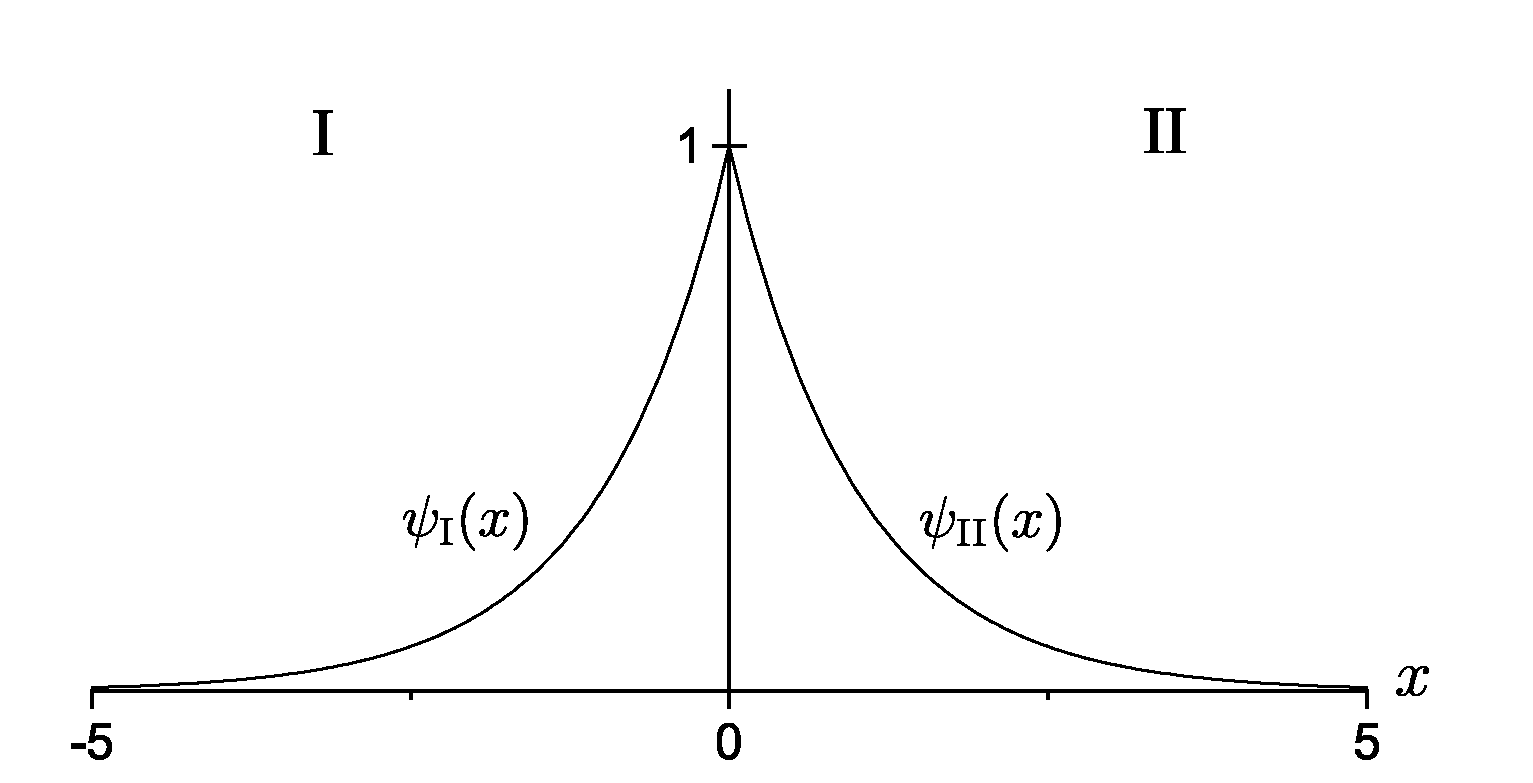
\epsfig{file=figures/deltapsi.eps,width=0.6\linewidth}
			\scaption{
				Normalizovaná vlnová funkce vázaného stavu pro $M=\hbar=1$, $c=-1$.
			}
			\label{fig:DeltaWF}
		\end{figure}
		
		Zbývá nanormovat vlnovou funkci, tj. nalézt hodnotu parametru $A$:
		\begin{align}
			1
			&=\int_{-\infty}^{\infty}\abs{\psi(x)}^{2}\d x
			 =\int_{-\infty}^{0}\abs{\psi_{\ti{I}}(x)}^{2}\d x
				+\int_{0}^{\infty}\abs{\psi_{\ti{II}}(x)}^{2}\d x\nonumber\\
			&=\abs{A}^{2}\left\{\int_{-\infty}^{0}\e^{2\kappa x}\d x
				+\int_{0}^{\infty}\e^{-2\kappa x}\d x\right\}\nonumber\\
			&=\abs{A}^{2}\left\{\left[\frac{1}{2\kappa}\e^{2\kappa x}\right]_{-\infty}^{0}
				+\left[-\frac{1}{2\kappa}\e^{-2\kappa x}\right]_{0}^{\infty}\right\}
			 =\frac{\abs{A}^{2}}{\kappa},
		\end{align}
		Při volbě nulové komplexní fáze normalizačního parametru je
		\begin{equation}
            A=D=\sqrt{\kappa}
                =\sqrt{-\frac{Mc}{\hbar^{2}}}
		\end{equation}
		[veličina $\kappa$ byla vyjádřena pomocí~\eqref{eq:Deltakappa} a~\eqref{eq:kappa}].
		Normalizovaná vlnová funkce vázaného stavu~\eqref{eq:DeltaEnergy} je tedy
		\begin{subequations}
			\begin{align}
				\psi_{\ti{I}}(x)
					&=\sqrt{-\frac{Mc}{\hbar^{2}}}\e^{-\frac{Mc}{\hbar^{2}} x},\\
				\psi_{\ti{II}}(x)
					&=\sqrt{-\frac{Mc}{\hbar^{2}}}\e^{\frac{Mc}{\hbar^{2}} x},
			\end{align}
		\end{subequations}
		nebo souhrnně
		\begin{equation}
			\psi(x)=\sqrt{-\frac{Mc}{\hbar^{2}}}\e^{-\frac{Mc}{\hbar^2}\abs{x}}.
		\end{equation}
		Její průběh je znázorněn na obrázku~\ref{fig:DeltaWF}.
		
	\item
		Jedná se o rozptylovou úlohu na 1D potenciálu.
		Částice přichází z oblasti, ve které je asymptoticky volná, do lokalizované interakční oblasti.
		Interakce způsobí, že se částice může s určitou nenulovou pravděpodobností odrazit. 
		Pokud naopak projde, může se změnit její fáze.
		Tyto změny udávají měřitelné veličiny pravděpodobnost průchodu $T$, pravděpodobnost odrazu $R$ a fázový posun $\delta$.

		V kladných energiích má systém spojité spektrum.
		V oblastech I a II je řešením Schödingerovy rovnice~\eqref{eq:DeltaWF} se vlnová funkce vyjádří jako
		\begin{subequations}
			\begin{align}
				\psi_{\ti{I}}(x)&=A\e^{\im k x}+B\e^{-\im k x},\nonumber\\
				\psi_{\ti{II}}(x)&=C\e^{\im k x}+D\e^{-\im k x},
			\end{align}
			\label{eq:DeltaBarrierWF}
		\end{subequations}
		kde
		\begin{equation}
			k=\sqrt{\frac{2ME}{\hbar^{2}}}.
			\label{eq:k}
		\end{equation}
		
		Pro určení pravděpodobností průchodu\index{pravděpodobnost!průchodu} a odrazu\index{pravděpodobnost!odrazu} se předpokládá, že k $\delta$ funkci přichází vlna zleva (člen úměrný $A$) a rozdělí se na odraženou vlnu (člen úměrný $B$) a prošlou vlnu (člen úměrný $D$).
		Zprava žádná vlna nepřichází, takže $D=0$.
		Hledané pravděpodobnosti se pak definují jako
		\begin{subequations}
			\begin{align}
				R&=\abs{\mathfrak{R}}^{2},
				&\mathfrak{R}&=\frac{B}{A},\\
				T&=\abs{\mathfrak{T}}^{2},
				&\mathfrak{T}&=\frac{C}{A}=\abs{T}\e^{\im\delta},
				\label{eq:PhaseShift}
			\end{align}
		\end{subequations}
		kde $\mathfrak{R}$ je \emph{amplituda odrazu},\index{amplituda!odrazu} $\mathfrak{T}$ je \emph{amplituda průchodu}\index{amplituda!průchodu} a $\delta$ je \emph{fázové posunutí}.\index{posunutí!fázové}

		\begin{figure}[!htbp]
			\centering
			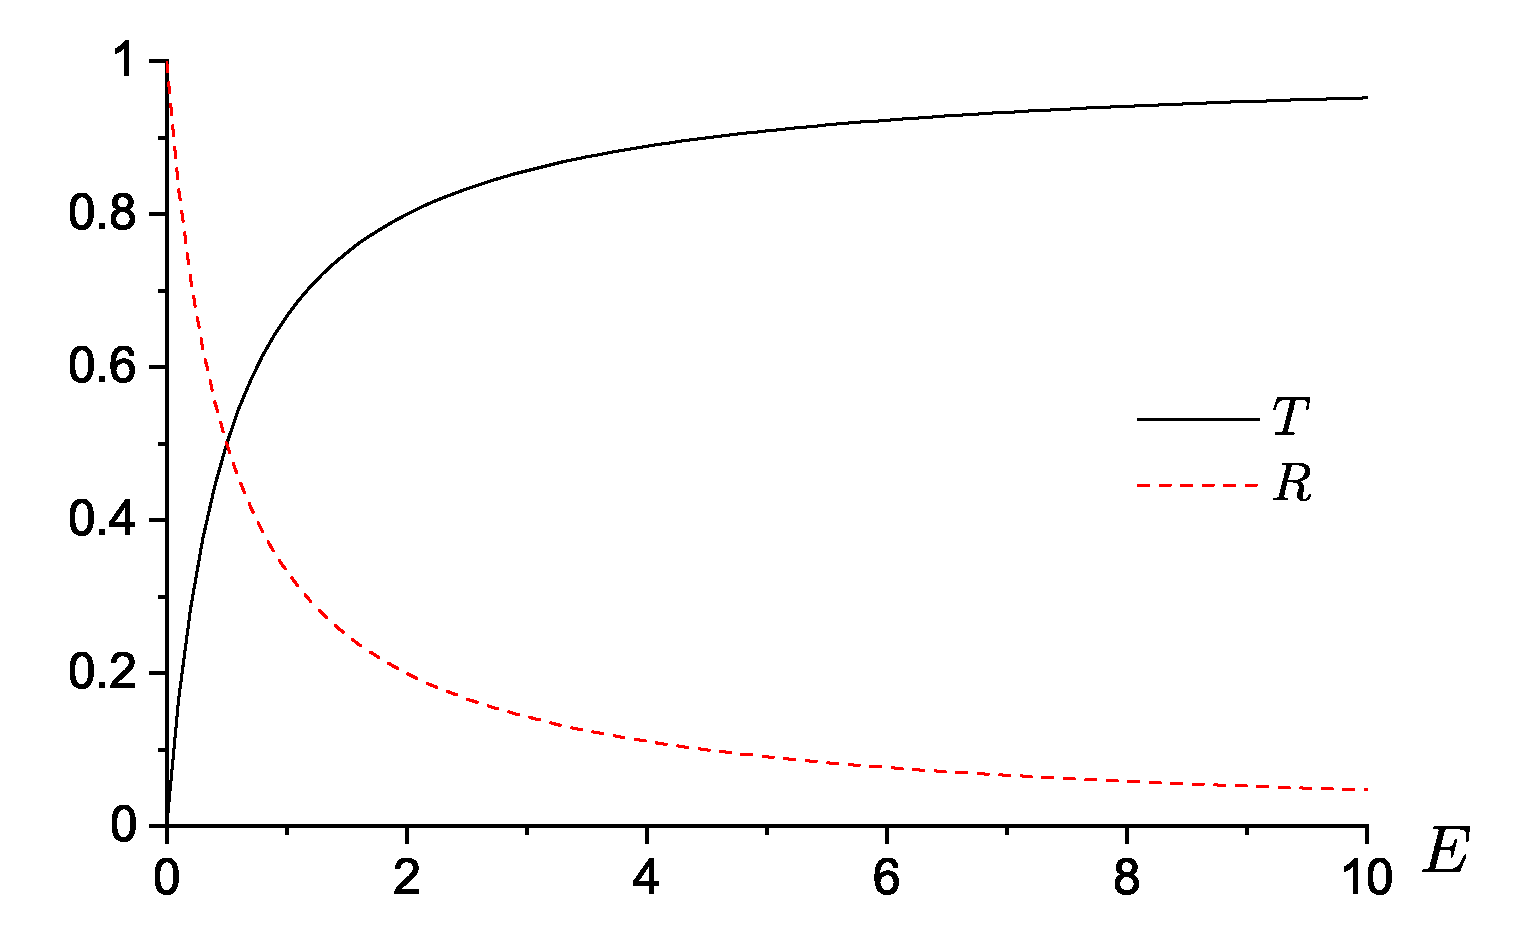
\epsfig{file=figures/deltatr.eps,width=0.6\linewidth}
			\scaption{
				Pravděpodobnost průchodu (černá čára) a odrazu (červená přerušovaná čára) pro potenciál tvořený jednou $\delta$ funkcí ($M=\hbar=c=1$).
                Jejich součet je roven 1.
			}
			\label{fig:DeltaTR}
		\end{figure}

		Sešívání vlnové funkce~\eqref{eq:DeltaBarrierWF} v bodě $x=0$ vede na podmínky
		\begin{subequations}
			\begin{align}
				A+B&=C,\\
				\im k(C+B-A)&=KC.
			\end{align}
		\end{subequations}
		Vyjádřením $B$ z první podmínky a dosazením do druhé se dostane
		\begin{equation}
			C=\frac{A}{1-\frac{K}{2ik}}.
		\end{equation}
		Pravděpodobnost průchodu je tedy
		\begin{equation}
			T=\frac{1}{1-\frac{K}{2ik}}\frac{1}{1+\frac{K}{2ik}}
			 =\frac{1}{1+\left(\frac{K}{2k}\right)^{2}}
			 =\frac{1}{1+\frac{Mc^{2}}{2\hbar^{2}E}}
			\label{eq:DeltaT}
		\end{equation}
		a analogicky pravděpodobnost odrazu
		\begin{equation}
			R=\frac{1}{1+\left(\frac{2K}{k}\right)^{2}}
			 =\frac{1}{1+\frac{2\hbar^{2}E}{Mc^{2}}}.
			\label{eq:DeltaR}
		\end{equation}
        Platí, že $T+R=1$. 
        Obě pravděpodobnosti jsou zakresleny na obrázku~\ref{fig:DeltaTR}.
        
        \begin{note}
            Povšiměte si, že $R$ ani $T$ nezávisejí na znaménku $c$, tj. pravděpodobnost průchodu a odrazu je při zadané energii stejná pro $\delta$ jámu i pro $\delta$ bariéru.
        \end{note}    
    					
	\item
		Fázové posunutí\sfootnote{
            Držíme se zavedené notace, proto pro fázové posunutí i pro $\delta$ funkci se používá stejné, přestože kolizní označení.} 
		$\delta$\index{posunutí!fázové} značí fázi, o kterou se posune rovinná vlna kvůli přítomnosti potenciálu oproti případu bez potenciálu.
		Situace je schematicky znázorněna na obrázku~\ref{fig:DeltaWFPhaseShift}.
		Pro určení fázového posunutí se vyjde z definice~\eqref{eq:PhaseShift}, což po dosazení dá
		\begin{equation}
			\delta=\arctan{\frac{\imaginary{\mathfrak{T}}}{\real{\mathfrak{T}}}}
				=-\arctan{\frac{K}{2k}}
				=-\arctan{c\sqrt{\frac{M}{2\hbar^{2}E}}}.
			\label{eq:DeltaPhaseShift}
		\end{equation}
		Energetická závislost fázového posunutí je zakreslena na obrázku~\ref{fig:DeltaPhaseShift}.

		\begin{figure}[!htbp]
			\centering
			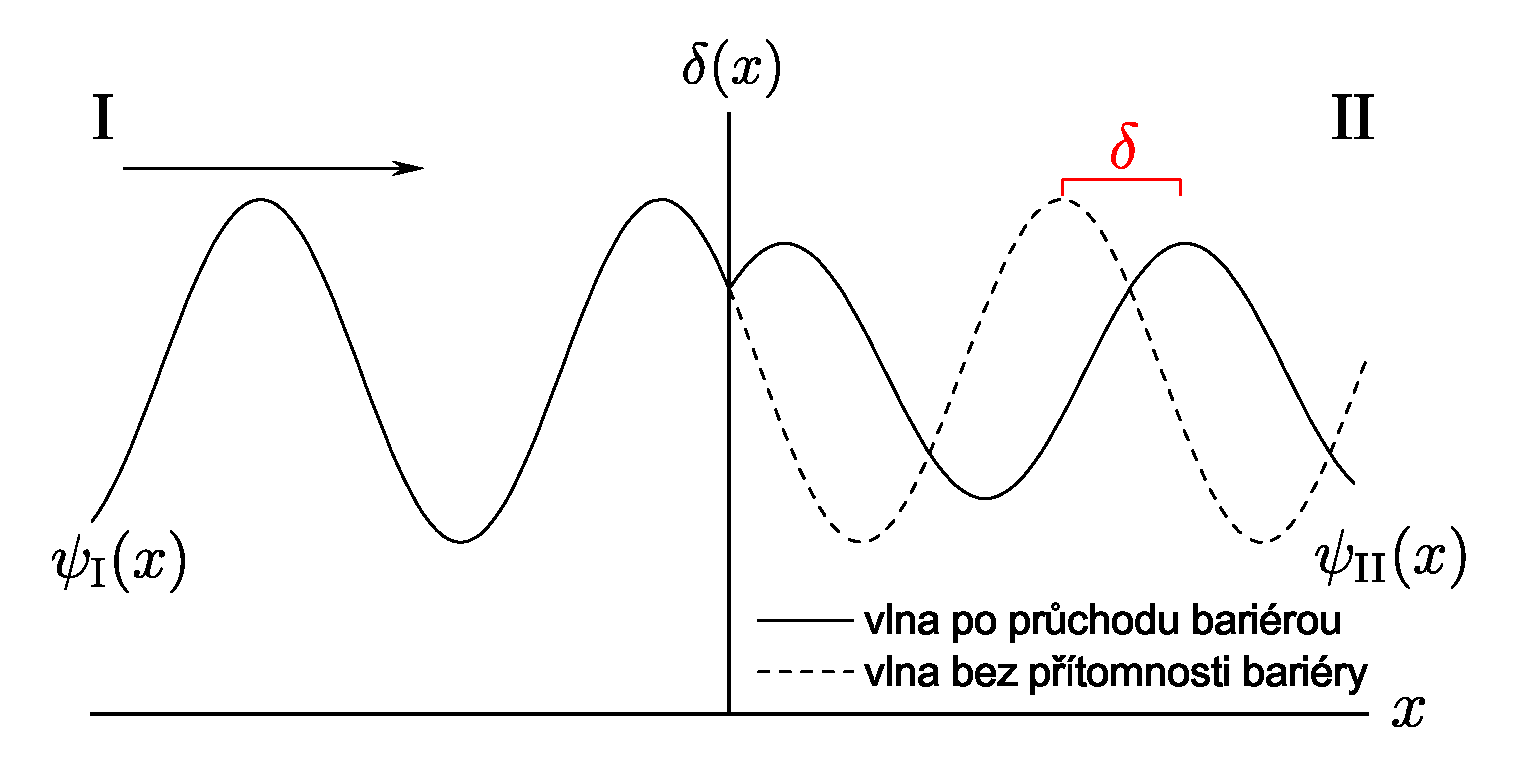
\epsfig{file=figures/deltasin.eps,width=0.7\linewidth}
			\scaption{
				Vlnová funkce pro výpočet fázového posunutí $\delta$ (červeně).
				Vlnová funkce za nepřítomnosti potenciálu $V(x)=c\,\delta(x)$ je znázorněna přerušovanou čarou.
			}
			\label{fig:DeltaWFPhaseShift}
		\end{figure}
		
		\begin{figure}[!htbp]
			\centering
			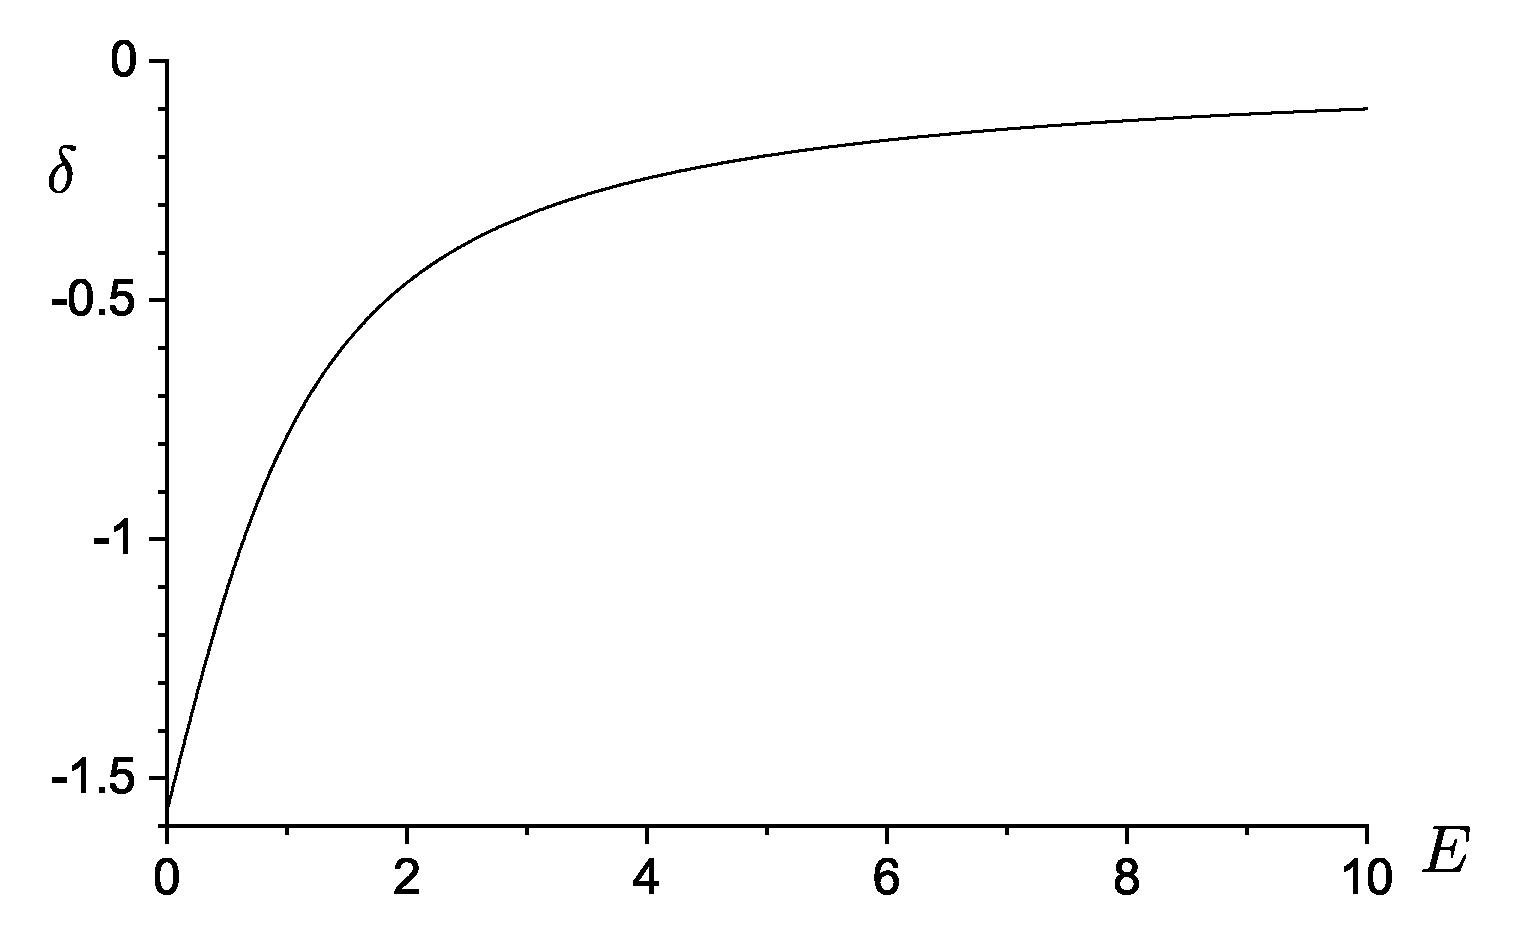
\epsfig{file=figures/deltadelta.eps,width=0.6\linewidth}
			\scaption{
				Fázové posunutí pro jednu $\delta$ funkci ($M=\hbar=c=1$).
			}
			\label{fig:DeltaPhaseShift}
		\end{figure}			
	\end{enumerate}	
\end{solution}

\begin{note}
    Potenciál ve tvaru $\delta$ funkce má simulovat velmi úzkou a hlubokou potenciálovou jámu, resp. bariéru.
    Jedná se vlastně o limitní případ konečné jámy (bariéry) šířky $a$ a hloubky (výšky) $v$, kde $a\rightarrow0$ a zároveň $va\equiv c=\const$.
\end{note}

\subsection{Dvě $\delta$ jámy nebo bariéry}\label{sec:DoubleDelta}
Částice o hmotnosti $M$ se pohybuje v potenciálu složeném ze dvou $\delta$ funkcí vzdálených od sebe o délku $a$,
\begin{equation}\label{eq:HamiltonianDoubleDelta}
    V(x)=c\left[\delta\left(x-\frac{a}{2}\right)+\delta\left(x+\frac{a}{2}\right)\right].
\end{equation}

\begin{enumerate}
\item
    Nalezněte rovnici pro vázané stavy systému ($E<0$, $c<0$) a vyřešte ji numericky.
    Porovnejte výsledné energetické spektrum s případem jedné jámy.
    
\item
    Pro $E>0$ určete pravděpodobnost průchodu $T(E)$ a pravděpodobnost odrazu $R(E)$.
    Zakreslete $T(E)$ do grafu společně s pravděpodobností průchodu skrz jednu $\delta$ funkci.
    
\item
    Pro $E>0$ určete fázové posunutí $\delta_{\pm}(E)$ zvlášť pro liché a zvlášť pro sudé vlnové funkce.
    Zakreslete obě fázová posunutí do grafu společně s fázovým posunutím pro jednu $\delta$ funkci.
\end{enumerate}

Pro všechny číselné výpočty uvažujte $\hbar=M=\abs{c}=a=1$.
	
\begin{solution}
	\begin{enumerate}
	\item
        Jelikož Hamiltonián~\eqref{eq:HamiltonianDoubleDelta} komutuje s operátorem parity $\operator{P}$, tj. je symetrický vůči záměně $x\leftrightarrow-x$, $p\leftrightarrow-p$, vlnové funkce $\psi(x)$ musejí být sudé nebo liché,        
		\begin{subequations}		
			\begin{align}
				\psi_{+}(x)&=\psi_{+}(-x): & \psi_{\ti{II}}(x)&=A_{+}\cosh{\kappa_{+} x}\\
					& &\psi_{\ti{III}}(x)&=B_{+}\e^{-\kappa_{+} x}=\psi_{\ti{I}}(-x)\\
				\psi_{-}(x)&=-\psi_{-}(-x): & \psi_{\ti{II}}(x)&=A_{-}\sinh{\kappa_{-} x}\\
					& &\psi_{\ti{III}}(x)&=B_{-}\e^{-\kappa_{-} x}=-\psi_{\ti{I}}(-x),
			\end{align}
		\end{subequations}
		kde $\kappa_{\pm}$ jsou dána vztahem~\eqref{eq:kappa}.
		Aplikace podmínky spojitosti v bodě $x=a/2$ a skoku v derivaci~\eqref{eq:SewDerivativeDelta} vede pro sudé řešení na rovnice
		\begin{subequations}
			\begin{align}
				A_{+}\cosh{\kappa_{+}\frac{a}{2}}
					&=B_{+}\e^{-\kappa_{+}\frac{a}{2}}\nonumber\\
				-B_{+}\kappa_{+}\e^{-\kappa_{+}\frac{a}{2}}-A_{+}\kappa_{+}\sinh{\kappa_{+}\frac{a}{2}}
					&=KB_{+}\e^{-\kappa_{+}\frac{a}{2}},
			\end{align}
			\label{eq:DoubleDeltaSewEven}
		\end{subequations}
		jejichž vydělením se obdrží kvantovací podmínka
		\begin{equation}\label{eq:DoubleDeltaEEven}
			\boxed{\kappa_{+}\tanh{\kappa_{+}\frac{a}{2}}
				=-\left(\kappa_{+}+K\right)}.
		\end{equation}
		Pro lichá řešení stačí provést záměnu $\sinh{x}\leftrightarrow\cosh{x}$, což vede na rovnici
		\begin{equation}\label{eq:DoubleDeltaEOdd}
            \boxed{\kappa_{-}\coth{\kappa_{-}\frac{a}{2}}
                =-\left(\kappa_{-}+K\right)}.
		\end{equation}
		Po vyjádření hyperbolických funkcí pomocí exponenciál
		\begin{equation}
            \tanh{x}
                =\frac{1}{\coth{x}}
                =\frac{\e^{x}-\e^{-x}}{\e^{x}+\e^{-x}}
		\end{equation}
		lze podmínky~\eqref{eq:DoubleDeltaEEven} a~\eqref{eq:DoubleDeltaEOdd} kompaktně zapsat jedinou rovnicí
		\begin{equation}\label{eq:DoubleDeltaE}
			\boxed{-K\e^{-\kappa_{\pm}a}=\pm\left(2\kappa_{\pm}+K\right)}.
		\end{equation}
		Řešením této rovnice je průsečík exponenciály $-K\e^{-\kappa{_{\pm}a}}$ (pro vázané stavy je $K<0$, takže exponenciála leží v horní polorovině grafu) s přímkami $\pm(2\kappa_{\pm}+K)$.
		Zatímco sudé řešení existuje vždy, existence lichého řešení je podmíněna tím, že směrnice přímky v bodě $\kappa_{-}=0$ musí být větší než směrnice exponenciály v tomtéž bodě:
		\begin{equation}
			\boxed{Ka<-2}.
		\end{equation}
		Obě situace jsou znázorněny na obrázku~\ref{fig:DoubleDeltaE}.
		
		\begin{figure}[!htbp]
            \begin{subfigure}{0.49\linewidth}
                \centering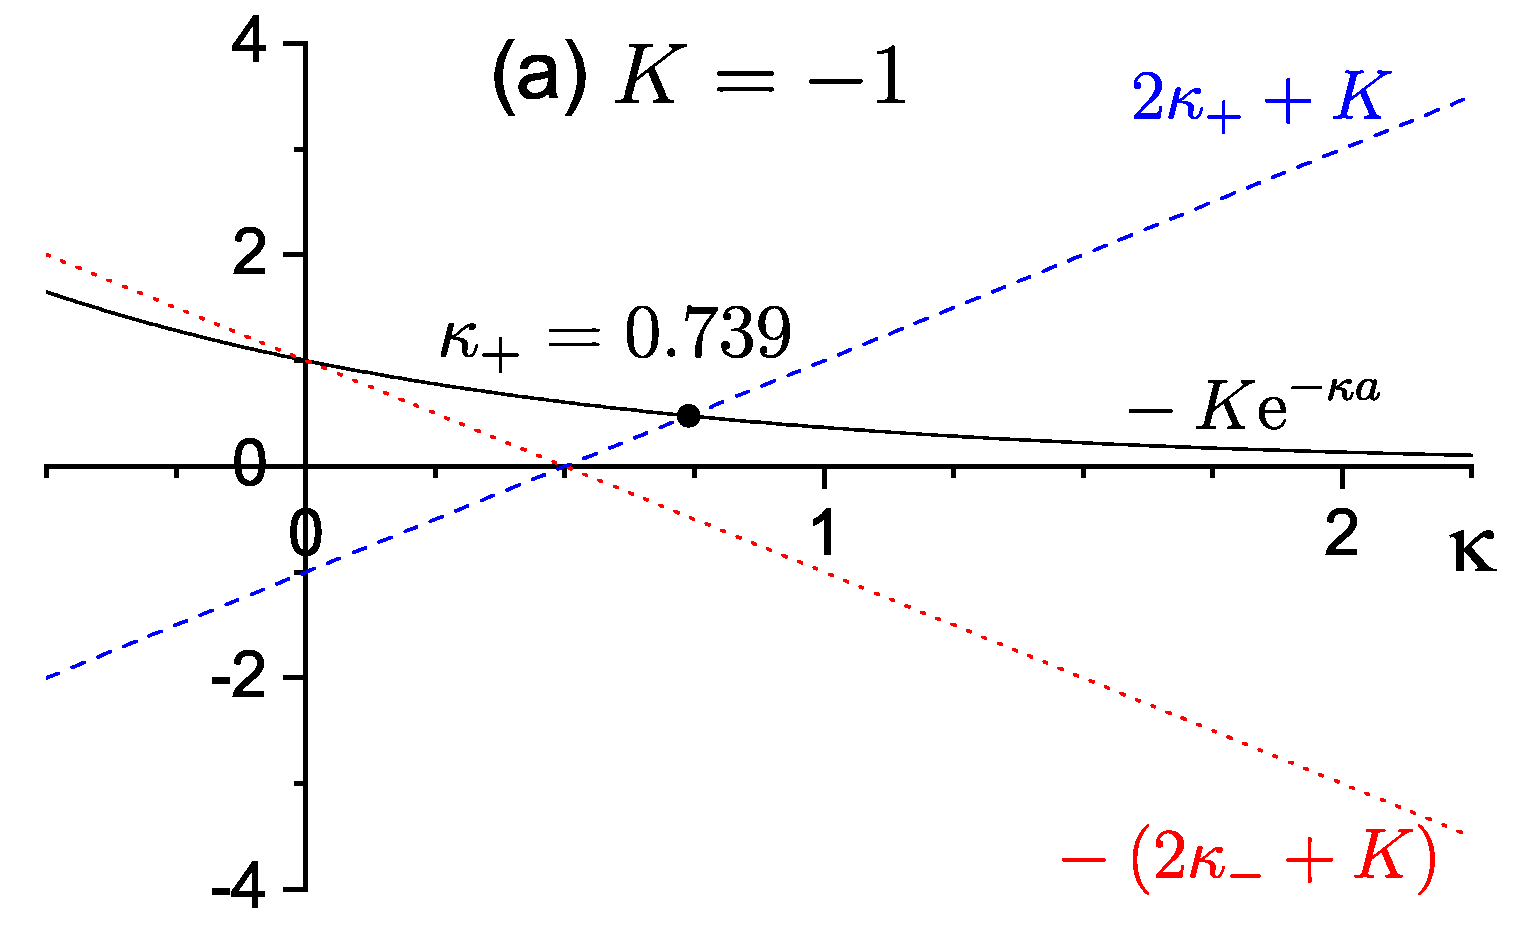
\epsfig{file=2deltak1.eps,width=\linewidth}
            \end{subfigure}
            \hfill
            \begin{subfigure}{0.49\linewidth}
                \centering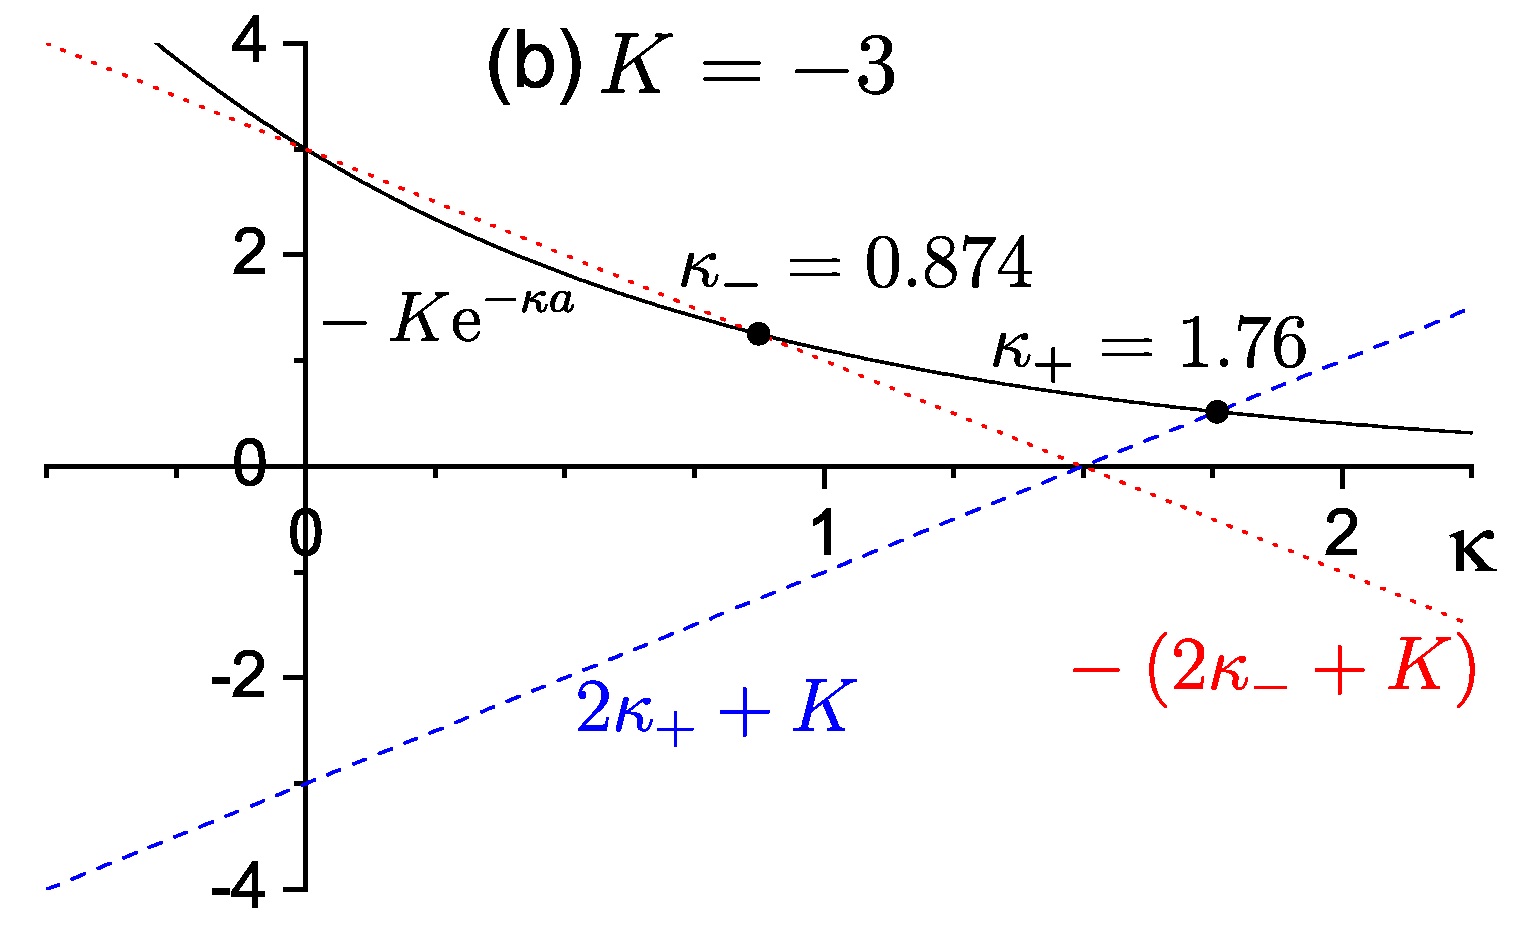
\epsfig{file=2deltak3.eps,width=\linewidth}
            \end{subfigure}
    
			\scaption{
				Numerické řešení rovnice~\eqref{eq:DoubleDeltaE} pro dvě hodnoty $K=-1$ a $K=-3$.
				V případě $K=-1$ existuje pouze sudé řešení s energií $E_{+}=-0.273$ (liché řešení $E_{-}=0$ vede na nenormalizovatelnou vlnovou funkci),
				v případě $K=-3$ existují dvě řešení $E_{+}=-1.55$ a $E_{-}=-0.382$.
			}
			\label{fig:DoubleDeltaE}
		\end{figure}		
		
		Řešení rovnic~\eqref{eq:DoubleDeltaE} lze explicitně vyjádřit pomocí \emph{Lambertových $W$ funkcí}\sfootnote{
			Lambertovy $W$ funkce jsou definovány jako řešení rovnice
			\begin{equation}
				y=x\e^{x}.
			\end{equation}
			V programu Mathematica se skrývají pod označením \href{https://reference.wolfram.com/language/ref/ProductLog.html}{ProductLog}.
		}\index{funkce!Lambertovy}
		\begin{equation}
            \kappa_{\pm}
                =-\frac{K}{2}+\frac{1}{a}\,W\left(\mp\frac{Ka}{2}\e^{\frac{Ka}{2}}\right).
		\end{equation}
		
		\begin{figure}[!htbp]
            \begin{subfigure}{0.49\linewidth}
                \centering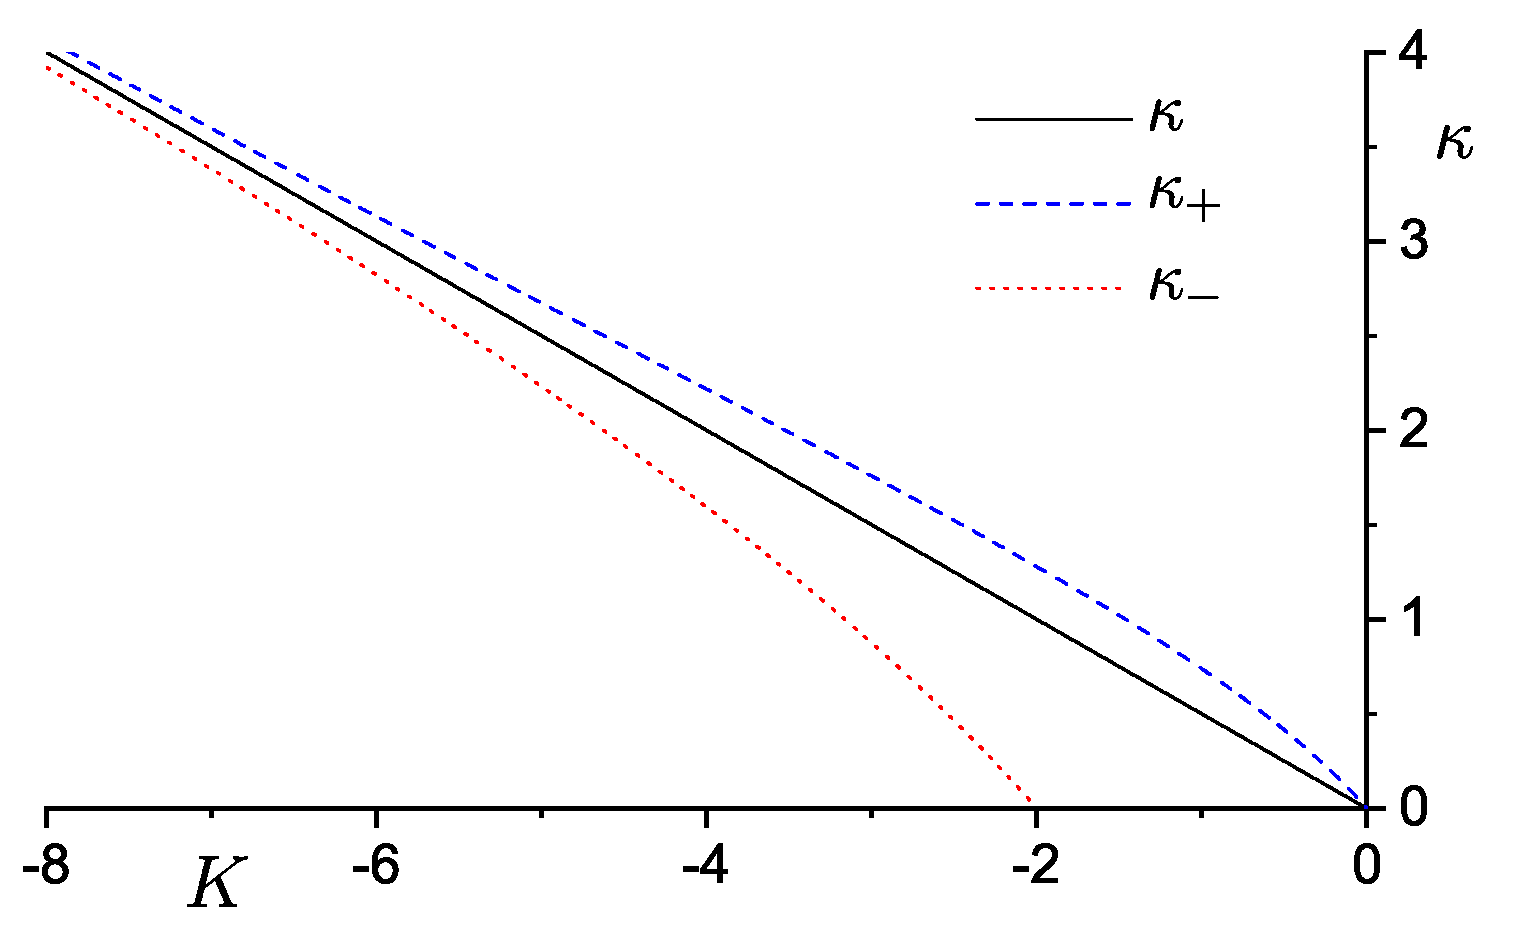
\epsfig{file=2deltaKk.eps,width=\linewidth}
            \end{subfigure}
            \hfill
            \begin{subfigure}{0.49\linewidth}
                \centering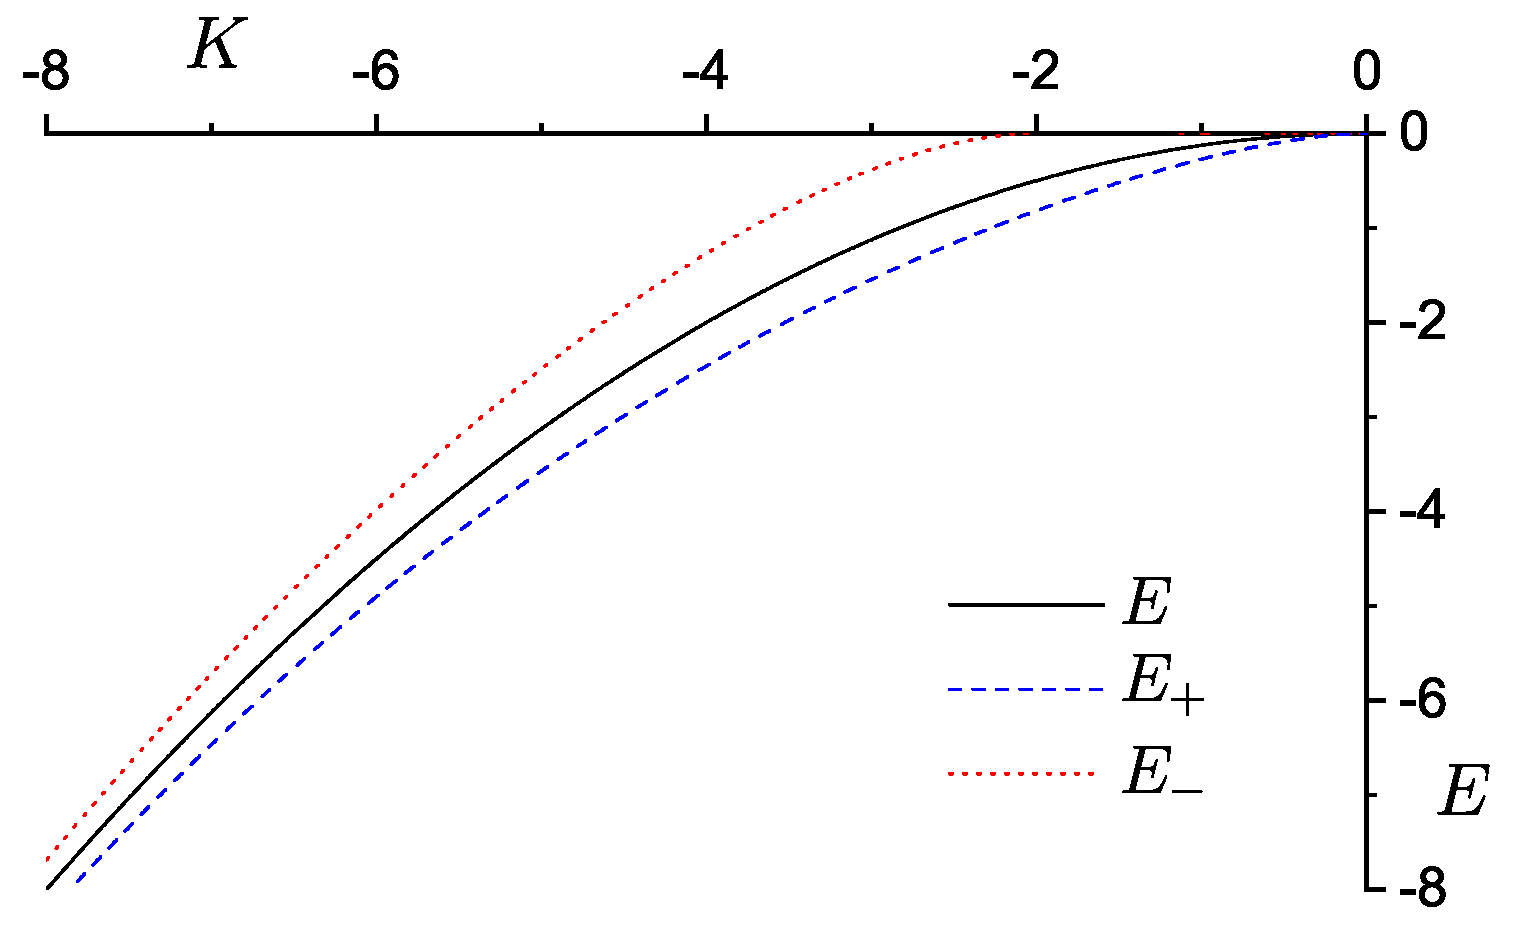
\epsfig{file=2deltaEk.eps,width=\linewidth}
            \end{subfigure}
			\scaption{
				Závislost spektra dvou $\delta$ jam $\kappa_{\pm}$ a $E_{\pm}$ na síle interakce $K$ a srovnání s jednou jámou $\kappa$ a $E$, viz~\eqref{eq:DeltaEnergy} a~\eqref{eq:DeltaK}.
			}
			\label{fig:DoubleDeltaLevelDynamics}
		\end{figure}		

		S klesající hodnotou $K$ (rostoucí silou $\delta$ funkcí v potenciálu) se řešení více a více přibližují k sobě.
		Pokud $Ka\ll0$, jámy popsané $\delta$ funkcemi mezi sebou jen velmi slabě interagují a energie budou tudíž téměř degenerované (paritní dublety) a budou blízké energii jedné $\delta$ jámy~\eqref{eq:DeltaEnergy} s dvojnásobnou silou $K$.
        Závislost řešení $\kappa_{\pm}(K)$ a odpovídajících energií $E_{\pm}(K)$ je vykreslena na obrázku~\ref{fig:DoubleDeltaLevelDynamics}.
		
		Normalizované vlnové funkce musejí splňovat normalizační podmínku
		\begin{equation}
			1=\int_{-\infty}^{\infty}\abs{\psi_{\pm}(x)}^{2}\d x
			 =2\int_{0}^{\infty}\abs{\psi_{\pm}(x)}^{2}\d x
		\end{equation}
        (druhá rovnost platí díky sudosti / lichosti vlnových funkcí).
        Sudé vlnové funkce jsou tedy
		\begin{align}
			\frac{1}{2}
				&=\int_{0}^{\frac{a}{2}}A_{+}^{2}\cosh^{2}{\kappa_{+}x}\d x
					+\int_{\frac{a}{2}}^{\infty}B_{+}^{2}\e^{-2\kappa_{+}x}\nonumber\\
				&=A_{+}^{2}\left[\frac{x}{2}+\frac{\sinh{2\kappa_{+}x}}{4\kappa_{+}}\right]
					_{0}^{\frac{a}{2}}+B_{+}^{2}\left[\frac{\e^{-2\kappa_{+}x}}{-2\kappa_{+}}\right]
					_{\frac{a}{2}}^{\infty}\nonumber\\
				&=\frac{A_{+}^{2}}{4\kappa_{+}}\left(\kappa_{+}a+\sinh{\kappa_{+}a}\right)
					+\frac{B_{+}^{2}}{2\kappa_{+}}\e^{-\kappa_{+}a}\nonumber\\
				&=\frac{A_{+}^{2}}{4\kappa_{+}}\left(\kappa_{+}a+\sinh{\kappa_{+}a}
					+2\cosh^{2}{\kappa\frac{a}{2}}\right)=\nonumber\\
				&=\frac{A_{+}^{2}}{4\kappa_{+}}\left(\e^{\kappa_{+}a}+\kappa_{+}a+1\right)
		\end{align}
		(v průběhu odvození byla použita sešívací podmínka~\eqref{eq:DoubleDeltaSewEven}), přičemž hodnoty parametrů $A_{+}$ a $B_{+}$ jsou
		\begin{subequations}
			\begin{align}
				A_{+}
					&=\sqrt{\frac{2\kappa_{+}}{\e^{\kappa_{+}a}+\kappa_{+}a+1}}
					=\sqrt{\frac{2(2\kappa_{+}+K)}{a(2\kappa_{+}+K)+2}},\nonumber\\
				B_{+}
					&=\frac{\e^{\kappa_{+}a}+1}{2}A_{+}
					=\frac{\kappa_{+}}{2\kappa_{+}+K}A_{+},
			\end{align}
		\end{subequations}
		kam se dosadilo z rovnice~\eqref{eq:kappa}.
		Liché vlnové funkce mají hodnoty parametrů
		\begin{subequations}
			\begin{align}
				A_{-}
					&=\sqrt{\frac{2\kappa_{-}}{\e^{\kappa_{-}a}-\kappa_{-}a-1}}
					=\sqrt{-\frac{2(2\kappa_{+}+K)}{a(2\kappa_{+}+K)+2}},\nonumber\\
				B_{-}
					&=\frac{\e^{\kappa_{+}a}-1}{2}A_{-}
					=-\frac{\kappa_{-}}{2\kappa_{+}+K}A_{-}.			
			\end{align}
		\end{subequations}
		Souhrnně lze tedy psát
		\begin{align}
			A_{\pm}&=\sqrt{\pm\frac{2(2\kappa_{+}+K)}{a(2\kappa_{+}+K)+2}}, & 
			B_{\pm}&=\pm\frac{\kappa_{-}}{2\kappa_{+}+K}A_{-}.			
		\end{align}
		
		\begin{figure}[!htbp]
            \begin{subfigure}{0.32\linewidth}
                \centering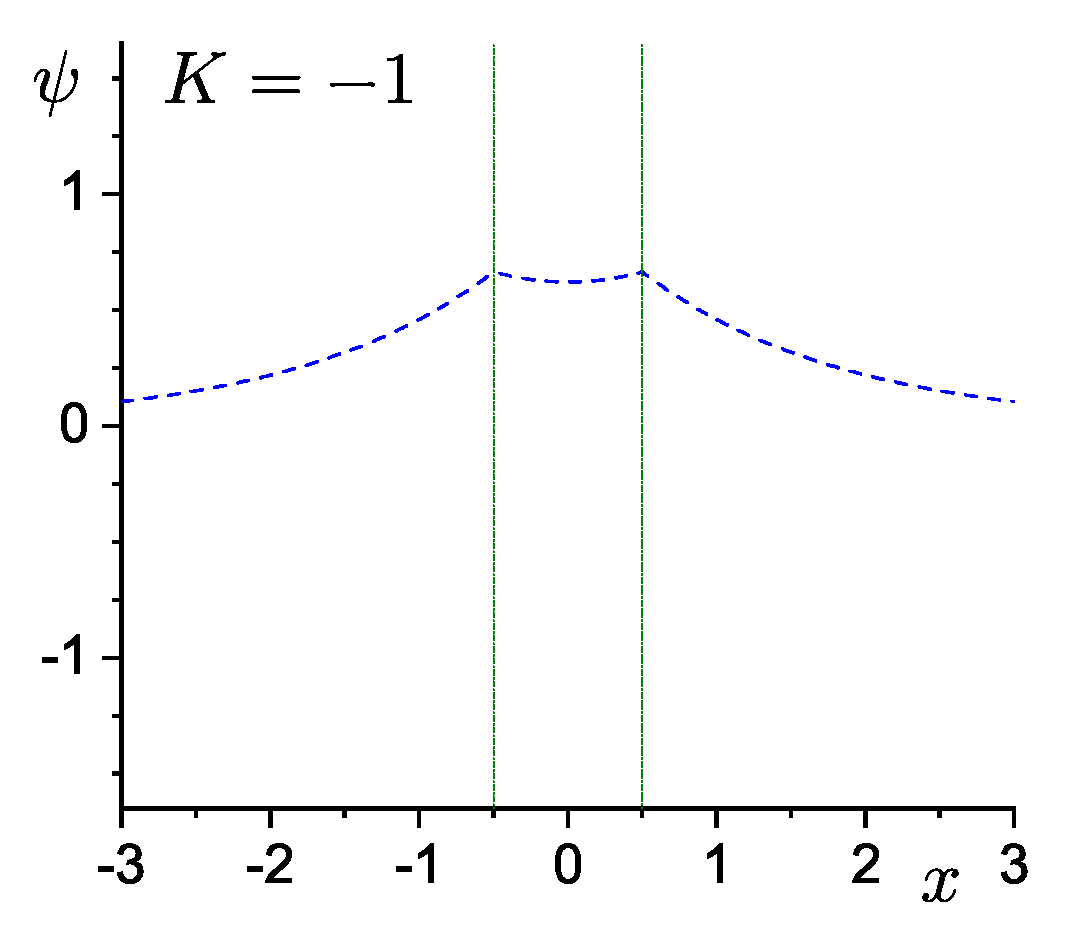
\epsfig{file=2deltapsi1.eps,width=\linewidth}
            \end{subfigure}
            \begin{subfigure}{0.32\linewidth}
                \centering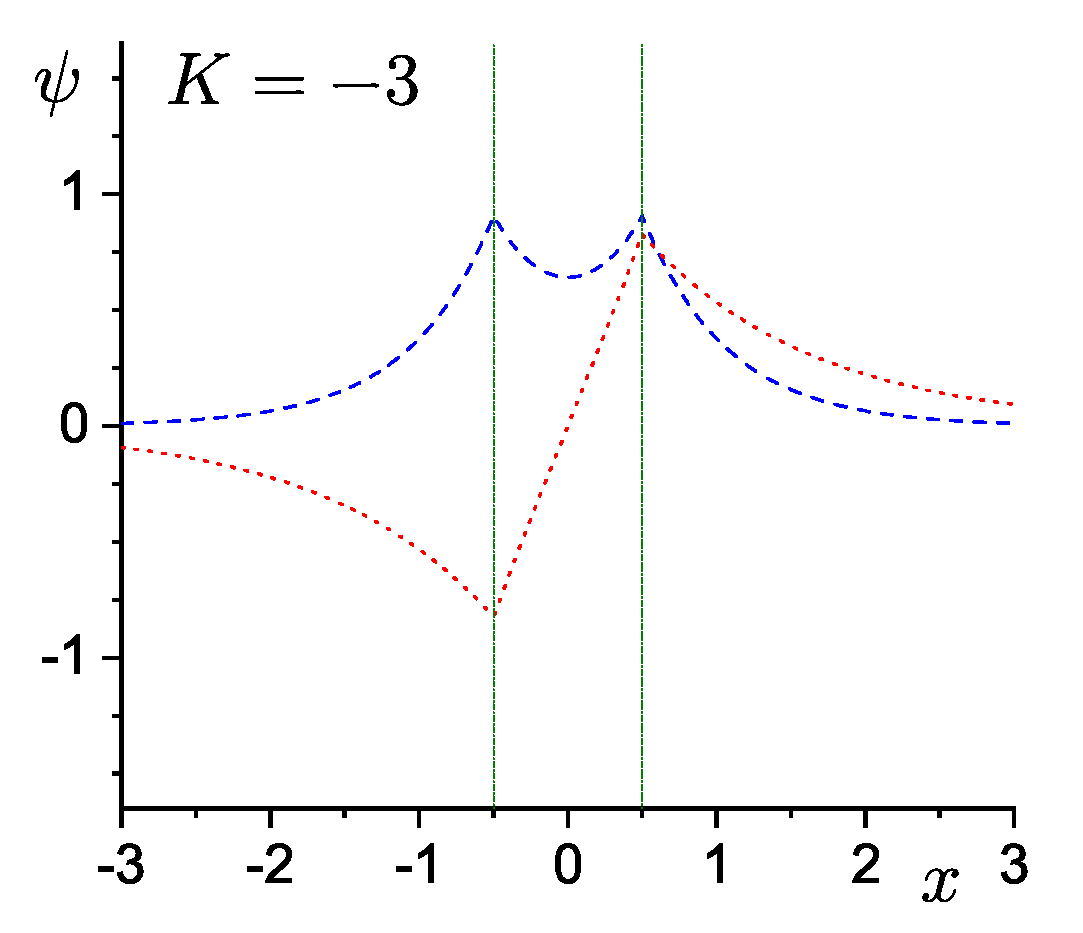
\epsfig{file=2deltapsi3.eps,width=\linewidth}
            \end{subfigure}
            \begin{subfigure}{0.32\linewidth}
                \centering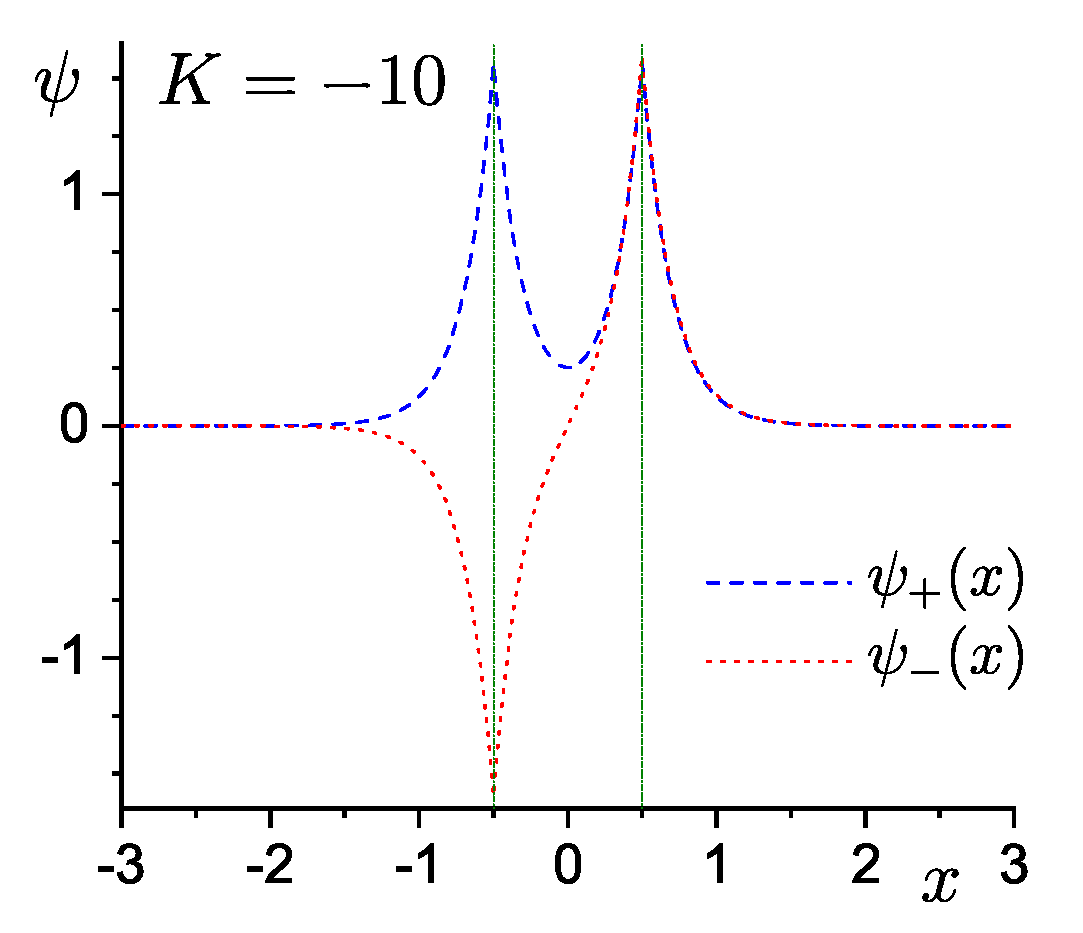
\epsfig{file=2deltapsi10.eps,width=\linewidth}
            \end{subfigure}
			\scaption{
				Normalizované vlnové funkce pro při hodnoty $K$.
				Pro $K=-1$ existuje jen jeden vázaný stav (sudá vlnová funkce), pro ostatní hodnoty $K$ existují dva vázané stavy: sudý $\psi_{+}(x)$ a lichý $\psi_{-}(x)$.
				Polohy $\delta$ funkcí jsou znázorněny svislými zelenými čerchovanými čarami.
			}
			\label{fig:DoubleDeltaWaveFunction}
		\end{figure}		

		Normalizované vlnové funkce pro tři různé hodnoty $K$ jsou zobrazeny na obrázku~\ref{fig:DoubleDeltaWaveFunction}.
		
	\item
		Pro stanovení pravděpodobnosti průchodu a odrazu se v analogii s~\eqref{eq:DeltaBarrierWF} opět vyjde z vlnové funkce ve tvaru (\trick{vlna přichází zleva})
		\begin{subequations}
			\begin{align}
				\psi_{\ti{I}}(x)
					&=A\e^{\im kx}+B\e^{-\im k x},\\
				\psi_{\ti{II}}(x)
					&=C\e^{\im kx}+D\e^{-\im k x},\\
				\psi_{\ti{III}}(x)
					&=F\e^{\im kx},
			\end{align}
		\end{subequations}
		kde $k$ je dáno vztahem~\eqref{eq:k}.
		Pravděpodobnost průchodu a odrazu bude
		\begin{equation}
            T=\abs{\frac{F}{A}}^{2},\qquad 
            R=\abs{\frac{B}{A}}^{2}.
		\end{equation}
		
		Podmínky spojitosti a skoku v derivaci vlnové funkce v bodě $\boxed{x=-a/2}$ vedou k rovnicím
		\begin{subequations}
			\begin{align}
				A\e^{-\im k\frac{a}{2}}+B\e^{\im k\frac{a}{2}}
					&=C\e^{-\im k\frac{a}{2}}+D\e^{-\im k\frac{a}{2}}\\
				\im k\left(C\e^{-\im k\frac{a}{2}}-D\e^{\im k\frac{a}{2}}
					-A\e^{-\im k\frac{a}{2}}+B\e^{+\im k\frac{a}{2}}\right)
					&=K\left(A\e^{-\im k\frac{a}{2}}+B\e^{\im k\frac{a}{2}}\right).		
			\end{align}
		\end{subequations}
		Z první rovnice vynásobené faktorem ${\im k}$ se vyjádří
		\begin{equation}\label{eq:DoubleDeltaCD1}
            C\im k\e^{-\im k\frac{a}{2}}
                =\im k\left(A\e^{-\im k\frac{a}{2}}+B\e^{\im k\frac{a}{2}}-D\e^{\im k\frac{a}{2}}\right)
		\end{equation}
		a tento výraz se dosadí do druhé rovnice, což po úpravách dá
		\begin{equation}
            \im k\left(B\e^{\im k\frac{a}{2}}-D\e^{\im k\frac{a}{2}}\right)
                =\frac{K}{2}\left(A\e^{-\im k\frac{a}{2}}+B\e^{\im k\frac{a}{2}}\right),
		\end{equation}
		a tedy
		\begin{equation}\label{eq:DoubleDeltaD1}
			D=\frac{\im K}{2k}\left(A\e^{-\im ka}+B\right)+B.
		\end{equation}
		Zpětným dosazením do~\eqref{eq:DoubleDeltaCD1} se dostane
		\begin{equation}\label{eq:DoubleDeltaC1}
			C=A-\frac{\im K}{2k}\left(A+B\e^{\im ka}\right).
		\end{equation}
		
		Analogický postup se zopakuje v bodě $\boxed{x=a/2}$, případně stačí vzít výsledek~\eqref{eq:DoubleDeltaD1} 
		a~\eqref{eq:DoubleDeltaC1} a provést záměnu $k\mapsto-k$, $A\mapsto F$, $B\mapsto 0$:
		\begin{align}\label{eq:DoubleDeltaCD2}
			C&=\frac{-K+2\im k}{2\im k}F &
			D&=-\frac{\im K}{2k}F\e^{\im ka}.
		\end{align}
		Zkombinování vztahů~\eqref{eq:DoubleDeltaD1}, \eqref{eq:DoubleDeltaC1} a \eqref{eq:DoubleDeltaCD2} vede na soustavu dvou rovnic pro neznámé $B$ a $E$:
		\begin{subequations}
			\begin{align}
				\frac{\im K}{2k}\left(A\e^{-\im ka}+B\right)+B
					&=-\frac{\im K}{2k}F\e^{\im ka},\\
				A-\frac{\im K}{2k}\left(A+B\e^{-\im ka}\right)
					&=\frac{-K+2\im k}{2\im k}F.
			\end{align}
		\end{subequations}
		Bez újmy na obecnosti lze volit $A=1$, čímž se vztahy pro pravděpodobnosti průchodu a odrazu zjednoduší na $T=\abs{F}^{2}$ a $R=\abs{B}^{2}$.
		
		Řešení posledních dvou rovnic zní
		\begin{equation}
			F=\frac{4k^{2}}{K^{2}\e^{2\im ka}-\left(K-2\im k\right)^{2}}.
			\label{eq:2DeltaF}
		\end{equation}
		Po úpravách se získá finální výraz pro pravděpodobnost průchodu
		\begin{align}
			T&=FF^{*}
				=\frac{4k^{2}}{K^{2}\e^{2\im ka}-\left(K-2\im k\right)^{2}}
					\frac{4k^{2}}{K^{2}\e^{-2\im ka}-\left(K+2\im k\right)^{2}}\nonumber\\
			 &=\frac{16k^{4}}{\underbrace{\left(K^{2}+4k^{2}\right)^{2}+K^{4}}
				_{2\clubsuit=2K^{4}+8K^{2}k^{2}+16k^{4}}-K^{2}\left[(K+2\im k)^{2}\e^{2\im ka}
				+\left(K-2\im k\right)^{2}\e^{-2\im ka}\right]}\nonumber\\
			 &=\frac{16k^{4}}{2\clubsuit-K^{2}\left[\left(K^{2}-4k^{2}\right)
				\left(\e^{2\im ka}+\e^{-2\im ka}\right)+4\im Kk\left(\e^{2\im ka}
				-\e^{-2\im ka}\right)\right]}\nonumber\\
			 &=\frac{16k^{4}}{2\clubsuit-K^{2}\left[2\left(K^{2}-4k^{2}\right)\cos{2ka}
				-8Kk\sin{2ka}\right]}\nonumber\\
			 &=\frac{8k^{4}}{\clubsuit-K^{2}\left[\left(K^{2}-4k^{2}\right)
				\left(\cos^{2}ka-\sin^{2}ka\right)-8Kk\sin{ka}\cos{ka}\right]}\nonumber\\
			 &=\frac{8k^{4}}{\clubsuit-K^{4}\cos^{2}ka+K^{4}\sin^{2}ka+4K^{2}k^{2}\cos^{2}ka
				-4K^{2}k^{2}\sin^{2}ka+8K^{3}k\sin{ka}\cos{ka}}\nonumber\\
			 &=\frac{4k^{4}}{4k^{4}+2K^{4}\sin{2}ka+8K^{2}k^{2}\cos^{2}ka
				+8K^{3}k\sin{ka}\cos{ka}}\nonumber\\
			 &=\frac{4k^{4}}{4k^{4}+K^{2}\left(K\sin{ka}+2k\cos{ka}\right)^{2}}\nonumber\\
			 &=\frac{1}{1+\frac{K^{2}}{4k^{2}}\left(2\cos{ka}+\frac{K}{k}\sin{ka}\right)^{2}}.
		\end{align}
        
        Srovnání s pravděpodobností průchodu pro jednu $\delta$ funkci~\eqref{eq:DeltaT} ukazuje, že v případě dvou $\delta$ funkcí se $T$ liší o modulační faktor v závorce ve jmenovateli.
		Ten způsobuje, že pro speciální hodnoty $k$ dané rovnicí
		\begin{equation}
			2\cos{ka}+\frac{K}{k}\sin{ka}=0,
		\end{equation}
		tj.
		\begin{equation}
            \tan{ka}
                =-\frac{2k}{K}
		\end{equation}		
		je pravděpodobnost průchodu $T=1$ a pravděpodobnost odrazu $R=0$.
		To je speciální případ tzv.~\emph{Ramsauerova-Townsendova efektu}\index{efekt!Ramsauerův-Townsendův}, viz též~\cite{Capri2002}, kapitola 4.10.
		Pravděpodobnost průchodu $T$ je pro dvě hodnoty $K$ zobrazena na obrázku~\ref{fig:DoubleDelta}~(a) a srovnána s případem pravděpodobnosti průchodu pro jednu $\delta$ funkci~\eqref{eq:DeltaT} s dvojnásobnou silou $K$ (limitní případ $a\rightarrow0$).
		Pravděpodobnost odrazu se dopočítá pomocí relace $R=1-T$.	
		
	\item
		Fázové posunutí se spočítá pomocí definičního vztahu~\eqref{eq:PhaseShift} z výrazu~\eqref{eq:2DeltaF}:
		\begin{align}
            F&=\frac{4k^{2}}{K^{2}\left(\cos{2ka}+\im\sin{2ka}\right)-\left(K-2\im k\right)^{2}}\nonumber\\
			 &=\frac{4k^{2}}{K^{2}(\cos{2ka}-1)+4k^{2}+\im K(K\sin{2ka}+4k)}\nonumber\\
			 &=\frac{4k^{2}\left[K^{2}(\cos{2ka}-1)+4k^{2}-\im K\left(K\sin{2ka}+4k\right)\right]}{\left[K^{2}(\cos{2ka}-1)+4k^{2}\right]^{2}+K^{2}\left(K\sin{2ka}+4k\right)^{2}},
		\end{align}
		\begin{equation}
			\delta=-\arctan\frac{\sin{2ka}+\frac{4k}{K}}{\cos{2ka}-1+\frac{4k^{2}}{K^{2}}}.
		\end{equation}
		Fázové posunutí je zobrazeno na obrázku~\ref{fig:DoubleDelta}~(b).
		Přitažlivý potenciál ($K<0$) dává fázové posunutí záporné, odpudivý potenciál ($K>0$) kladné.
		
		\begin{figure}[!htbp]
            \begin{subfigure}{0.49\linewidth}
                \centering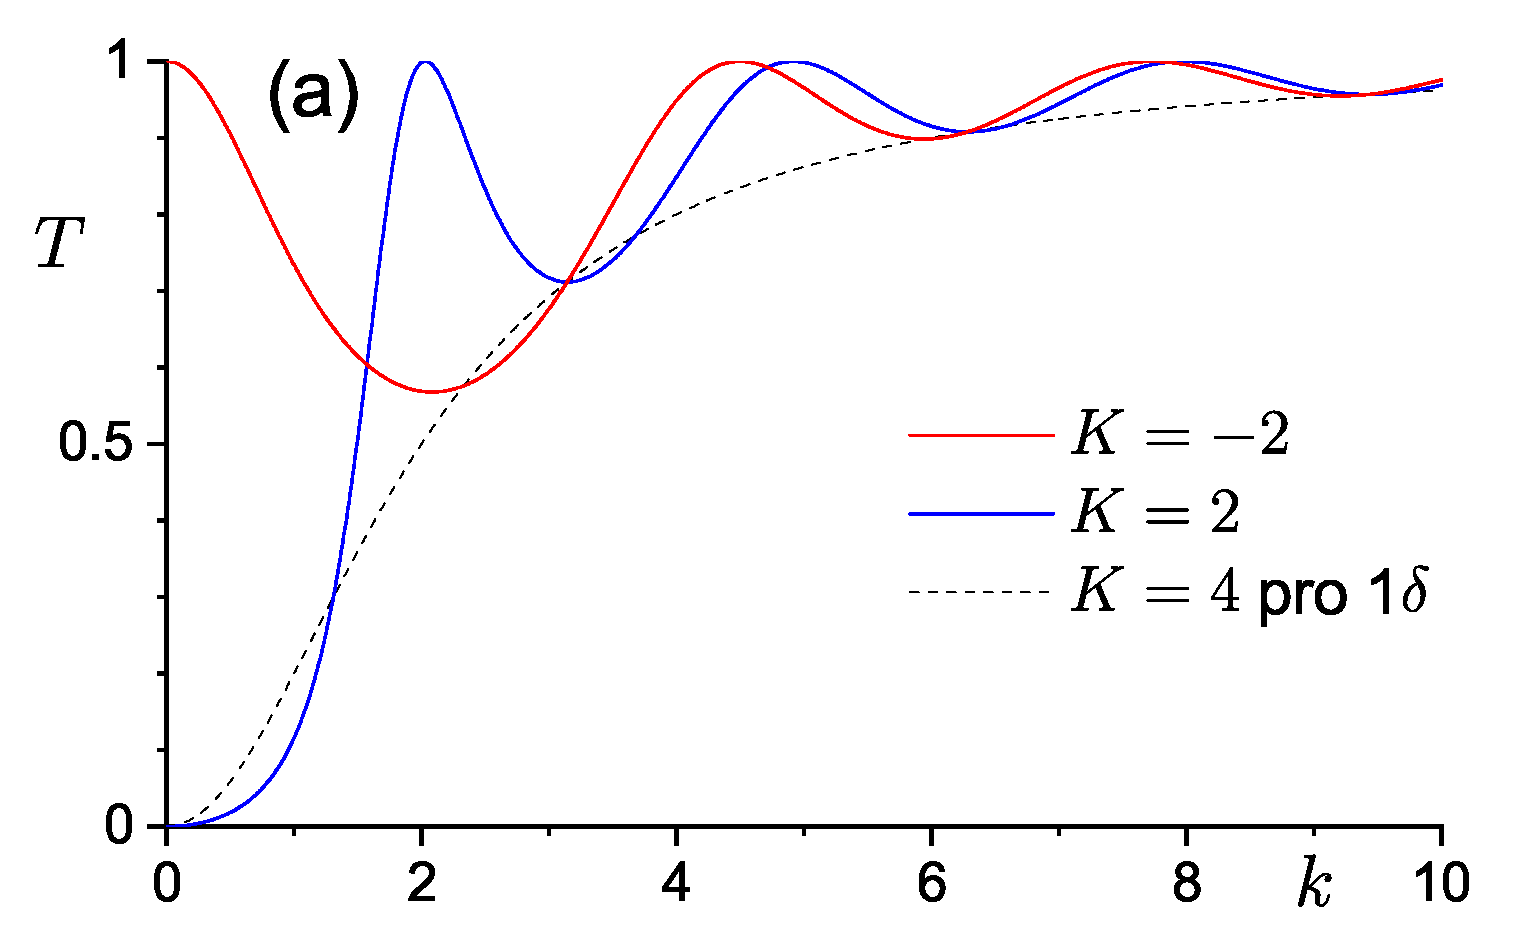
\epsfig{file=2deltaT.eps,width=\linewidth}
            \end{subfigure}
            \hfill
            \begin{subfigure}{0.49\linewidth}
                \centering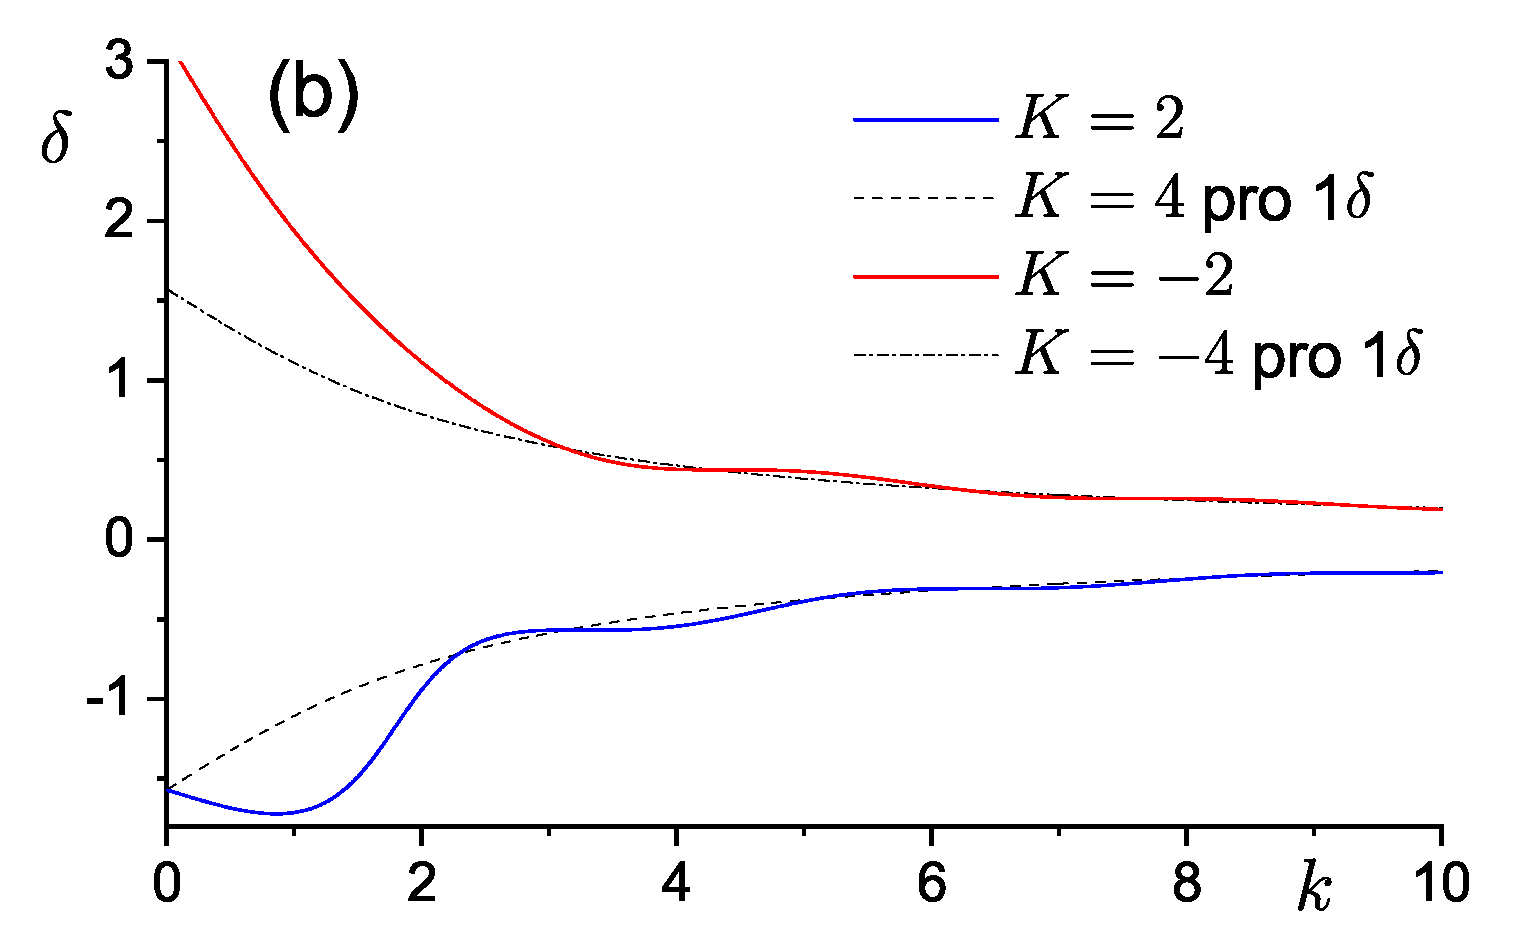
\epsfig{file=2deltadelta.eps,width=\linewidth}
            \end{subfigure}
			\scaption{
				(a) Pravděpodobnost průchodu a (b) fázové posunutí $\delta$ pro potenciál dvou $\delta$ jam s $K=-2$ (červeně) a $K=2$ (modře).
				Pro srovnání s případem jedné jámy síly $K=\pm4$ slouží černá čárkovaná čára 
				(v případě jedné jámy je pravděpodobnost průchodu stejná pro obě znaménka $K$).
			}			
			\label{fig:DoubleDelta}
		\end{figure}		
				
	\end{enumerate}
\end{solution}
\subsection{Maticový formalismus}
Částice hmotnosti $M$ se pohybuje v jednorozměrném potenciálu složeném z $n$ různě silných $\delta$ funkcí,
\begin{equation}\label{PotentialSumDelta}
    V(x)=\sum_{j=1}^{n}c_{j}\,\delta(x-x_{j}),
\end{equation}
kde $c_{j}$ jsou jejich \uv{síly} a $x_{1}<x_{2}<\dotsb<x_{n}$ jejich polohy.

\begin{enumerate}
\item
    Obecnou vlnovou funkci pro částici v bodě $x$ zapište ve formě dvousložkového vektoru.
    
\item
    Nalezněte transformaci posunutí vlnové funkce o vzdálenost $a$ a zapište tuto transformaci ve formě matice.
    
\item
    Nalezněte transformaci vlnové funkce při průchodu $\delta$ funkcí v bodě $x_{j}$.
    
\item
    Nalezněte transformaci $\Xi$, která dává do vztahu vlnovou funkci před první jámou s vlnovou funkcí po poslední jámě.
    
\item
    Pro případ dvou stejně silných jam vzdálených od sebe $a$ najděte podmínku na to, aby vlnová funkce pro vázané stavy $E<0$ byla normalizovatelná.
\end{enumerate}
	
\begin{solution}
	\begin{enumerate}
	\item
		Až na jednotlivé body $x_{j}$ se jedná o vlnovou funkci volné částice
		\begin{equation}\label{eq:SumDeltaWaveFunction}
			\psi(x)
				=\underbrace{A_{+}\e^{\im k x}}_{\psi_{+}(x)}
					+\underbrace{A_{-}\e^{-\im k x}}_{\psi_{-}(x)},
		\end{equation}
		kde $k=\sqrt{2ME/\hbar^{2}}$ [pro vázané stavy $E<0$ je $k$ ryze imaginární, nebo je možné přejít k veličině $\kappa$~\eqref{eq:kappa}].
		Vlnová funkce se zapíše v kompaktním tvaru dvousložkového vektoru
		\begin{equation}
			\Psi(x)\equiv\makematrix{\psi_{+}(x) \\ \psi_{-}(x)}.
		\end{equation}
		
	\item
		Posunutá vlnová funkce je
		\begin{equation}
			\psi(x+a)
				=A_{+}\e^{\im kx+\im ka}+A_{-}\e^{-\im kx-\im ka}
				=\e^{+\im ka}\psi_{+}(x)+\e^{-\im ka}\psi_{-}(x),
		\end{equation}
		takže
		\begin{equation}
			\Psi(x+a)
				=\makematrix{\e^{+\im ka}\psi_{+}(x) \\ \e^{-\im ka}\psi_{-}(x)}
				=\underbrace{\makematrix{\e^{+\im ka} & 0 \\ 0 & \e^{-\im ka}}}_{\matrix{T}(a)}\Psi(x)\,.
		\end{equation}
		
	\item
		\trick{Sešívací podmínka~\eqref{eq:SewDerivativeDelta} pro vlnovou funkci~\eqref{eq:SumDeltaWaveFunction} je lineární, a proto ji lze rovněž vyjádřit maticovou transformací vektoru $\Psi(x)$.}
		Označí-li se vlnová funkce nalevo od $j$-té $\delta$ funkce jako $\Psi^{(L)}(x_{j})$ a vlnová funkce napravo od $\delta$ funkce jako $\Psi^{(R)}(x_{j})$, pak podmínka na spojitost a na skok v derivaci v bodě $x_{j}$ zní
		\begin{subequations}
			\begin{align}
				\psi_{+}^{(L)}+\psi_{-}^{(L)}
					&=\psi_{+}^{(R)}+\psi_{-}^{(R)},\\
				\im k\left(\psi_{+}^{(R)}-\psi_{-}^{(R)}+\psi_{+}^{(L)}-\psi_{-}^{(L)}\right)
					&=K_{j}\left(\psi_{+}^{(L,R)}+\psi_{-}^{(L,R)}\right).
			\end{align}
		\end{subequations}
		Z první rovnice plyne $\psi_{-}^{(R)}=\psi_{+}^{(L)}+\psi_{-}^{(L)}-\psi_{+}^{(R)}$, což po dosazení do druhé rovnice dá
		\begin{subequations}
			\begin{align}
				\psi_{+}^{(R)}
					&=\frac{K_{j}}{2\im k}\left(\psi_{+}^{(L)}+\psi_{-}^{(L)}\right)+\psi_{+}^{(L)}
					=\left(1+\frac{K_{j}}{2\im k}\right)\psi_{+}^{(L)}+\frac{K_{j}}{2\im k}\psi_{-}^{(L)},\\
				\psi_{+}^{(L)}
					&=-\frac{K_{j}}{2\im k}\left(\psi_{+}^{(L)}+\psi_{-}^{(L)}\right)+\psi_{-}^{(L)}
					=-\frac{K_{j}}{2\im k}\psi_{+}^{(L)}+\left(1-\frac{K_{j}}{2\im k}\right)\psi_{-}^{(L)}.
			\end{align}
		\end{subequations}
		To je lineární transformace, kterou lze zapsat jako
		\begin{equation}
			\Psi^{(R)}(x_{j})
				=\underbrace{\makematrix{1+\frac{K_{j}}{2\im k} & \frac{K_{j}}{2\im k} 
								\\ -\frac{K_{j}}{2\im k} & 1-\frac{K_{j}}{2\im k}}}_{\matrix{R}\left(K_{j}\right)}
					\Psi^{(L)}(x_{j}).
		\end{equation}
		
		\item
			Transformace $\Xi$ je složením transformací posunutí mezi $\delta$ funkcemi $\matrix{T}$ 
			a transformací přechodu přes $\delta$ funkce $\matrix{R}$:
			\begin{equation}\label{eq:SumDeltaTransformationMatrix}
				\Xi(x_{n};x_{1})
					=\matrix{R}(K_{n})\matrix{T}(x_{n}-x_{n-1})\matrix{R}(K_{n-1})\dotsb\matrix{R}(K_{2})\matrix{T}(x_{2}-x_{1})\matrix{R}(K_{1}).
			\end{equation}			
			
		\item
			Transformace~\eqref{eq:SumDeltaTransformationMatrix} má pro dvě $\delta$ funkce tvar
			\begin{align}
				\Xi(a)
					&=\matrix{R}(K)\matrix{T}(a)\matrix{R}(K)\nonumber\\
					&=\makematrix{1+\frac{K}{2\pi k} & \frac{K}{2\im k} 
						\\ -\frac{K}{2\im k} & 1-\frac{K}{2\im k}}
						\makematrix{\e^{\im ka} & 0 \\ 0 & \e^{-\im ka}}
						\makematrix{1+\frac{K}{2\pi k} & \frac{K}{2\im k} 
						\\ -\frac{K}{2\im k} & 1-\frac{K}{2\im k}}\nonumber\\
					&=\makematrix{\left(1+\frac{K}{2\im k}\right)^{2}\e^{\im ka}
								-\left(\frac{K}{2ik}\right)^{2}\e^{-\im ka} &
							\frac{K}{2\im k}\left[\left(1+\frac{K}{2\im k}\right)\e^{\im ka}
								+\left(1-\frac{K}{2\im k}\right)\e^{-\im ka}\right] \\
							-\frac{K}{2\im k}\left[\left(1+\frac{K}{2\im k}\right)\e^{\im ka}
								+\left(1-\frac{K}{2\im k}\right)\e^{-\im ka}\right] &
							-\left(\frac{K}{2ik}\right)^{2}\e^{\im ka}
							+\left(1-\frac{K}{2\im k}\right)^{2}\e^{\im ka}}.
			\end{align}
			Stav bude normalizovatelný, pokud $\psi_{+}^{(L)}=\psi_{-}^{(R)}=0$, kde $\psi_{+}^{(L)}$ zde značí část vlnové funkce s kladným znaménkem nalevo před levou $\delta$ funkcí a $\psi_{-}^{(R)}$ část vlnové funkce napravo za pravou $\delta$ funkcí potenciálu.\sfootnote{
				Pro vázané stavy je $k=\im\sqrt{-2ME/\hbar}=\im\kappa$.
			}
			Jelikož $\Psi^{(R)}=\Xi\Psi^{(L)}$, platí
			\begin{equation}
                \psi_{-}^{(R)}
                    =\Xi_{21}\psi_{+}^{(L)}+\Xi_{22}\psi_{-}^{(L)},
			\end{equation}
			a pokud se kvůli správnému asymptotickému chování má vynulovat $\psi_{+}^{(L)}$ a $\psi_{-}^{(R)}$, musí být $\Xi_{22}=0$, neboli (po zavedení $k=\im\kappa$)
			\begin{equation}
				-\left(\frac{K}{2\kappa}\right)^{2}\e^{-\kappa a}
					+\left(1+\frac{K}{2\kappa}\right)^{2}\e^{\kappa a}=0,
			\end{equation}
			\begin{subequations}
				\begin{align}
					K^{2}\e^{-2\kappa a}
						&=\left(K+2\kappa\right)^{2},\\
					\abs{K}\e^{-\kappa a}
						&=\pm\left(K+2\kappa\right).
				\end{align}					
			\end{subequations}
			Rovnice je identická s rovnicemi~\eqref{eq:DoubleDeltaEEven} a ~\eqref{eq:DoubleDeltaEOdd}.
			Jejím řešením bychom dostali energie vázaných stavů.
	\end{enumerate}
\end{solution}

\subsection{Periodická $\delta$ funkce (Diracův hřeben)}\label{sec:DiracComb}
Částice o hmotnosti $M$ se pohybuje v jednorozměrné mřížce popsané periodickým potenciálem
\begin{equation}
    V(x)=c\sum_{n=-\infty}^{\infty}\delta(x-na),
\end{equation}
kde $a$ je vzdálenost mezi sousedními $\delta$ funkcemi (mřížková konstanta).

Hledejte vlnovou funkci ve tvaru Blochovy vlny 
\begin{equation}
    \psi_{q}(x)=\e^{\im q x}u_{q}(x),
    \label{eq:BlochWave}
\end{equation}
kde funkce $u_{q}(x)$ je periodická s periodou $a$
\begin{equation}
    u_{q}(x)=u_{q}(x+a)
    \label{eq:BlochTheorem}
\end{equation}
a $q$ je \emph{kvazihybnost (mřížková hybnost)}.\index{kvazihybnost}\index{hybnost!mřížková}\footnote{
    Někdy se též nazývá \emph{Floquetův exponent}.
}

\begin{enumerate}
\item
    Aplikujte sešívací podmínky pro navazování vlnové funkce na $\delta$ funkci a nalezněte energetické spektrum pro $c>0$, $E>0$.
    Diskutujte jeho vlastnosti a závislost na parametru $c$.

\item 
    Pro dvě hodnoty $K=1$ a $K=10$ vypočítejte a zakreslete do grafu disperzní relaci $E(q)$ pro nejnižší čtyři energetické pásy.
    Uvažujte následující konvenci: pokud $\pi n\leq ka\leq\pi(n+1)$, pak $\pi n\leq qa\leq\pi(n+1)$, $n\in\mathbb{N}$.

\item
    Vypočítejte grupovou rychlost
    \begin{equation}\label{eq:DiracCombGroupVelocity}
        v_{g}=\partialderivative{\omega}{q}
             =\frac{1}{\hbar}\partialderivative{E}{q}
    \end{equation}	
    a zakreslete její závislost na $q$ a na $E$ pro dvě hodnoty parametru $K=1$, $K=10$ a nejnižší čtyři energetické pásy.
    Srovnejte s rychlostí volné částice.

\item 
    Nalezněte parametry $A$, $B$ vlnové funkce. Vlnovou funkci normalizujte na vzdálenosti mezi dvěma delta funkcemi:
    \begin{equation}\label{eq:DiracCombWaveFunctionNormalization}
        \int_{0}^{a}\abs{\psi_{q}(x)}^{2}\d x=1.
    \end{equation}

\item
    Najděte řešení Schrödingerovy rovnice pro případ $K<0$ (v tomto případě může být energie i záporná).
    Podobně jako v 2. bodě zakreslete disperzní relaci $E(q)$ pro $K=-1$ a $K=-10$.

\end{enumerate}

Pro všechny numerické výpočty předpokládejte $a=M=\hbar=1$.

\begin{note}
    Diracův hřeben je triviální jednorozměrný model, na kterém lze studovat základní vlastnosti pohybu elektronů v pevné látce (pásová struktura, disperzní relace).
    Obecnější jednorozměrný potenciál, který místo opakujících se $\delta$ funkcí uvažuje pravoúhlé bariéry o konečné šířce $b$ a výšce $V_{0}$, vzdálené od sebe o mřížkovou konstantu $a>b$, se nazývá \emph{Kronigův-Penneyův potenciál}~\cite{Kronig1931}.\index{model!Kronigův-Penneyův}
    V limitě
    \begin{equation}
        b\rightarrow0,V_{0}\rightarrow\infty,bV_{0}=c=\const
    \end{equation}
    přejde Kronigův-Penneyův potenciál na Diracův hřeben.
\end{note}

\begin{solution}
	\begin{enumerate}
	\item
		Vlnová funkce na intervalu $x\in(0;a)$ odpovídá vlnové funkci volné částice
		\begin{equation}
			\psi_{q}^{(0;a)}(x)
                =A\e^{\im k x}+B\e^{-\im k x},\qquad 
            k\equiv\sqrt{\frac{2ME}{\hbar^{2}}}.
		\end{equation}
        Vyjádřená v Blochově formě podle~\eqref{eq:BlochWave} zní
        \begin{equation}
			\psi_{q}^{(0;a)}(x)
                =\e^{\im q x}\underbrace{\left(A\e^{-\im q x}\e^{\im k x}+B\e^{-\im q x}\e^{-\im k x}\right)}_{u_{q}(x)}.
        \end{equation}
        Podle Blochova teorému~\eqref{eq:BlochTheorem} lze využít \trick{periodicity} funkce $u_{q}(x)$ a posunout vlnovou funkci na interval $x\in(-a;0)$,\sfootnote{
			Zapůsobíme-li na Blochovu vlnu~\eqref{eq:BlochWave} operátorem posunutí
			$\operator{T}(a)=\e^{-\frac{\im}{\hbar}a\operator{p}}$, který byl zaveden vztahem~\eqref{eq:TranslationOperator}, dostaneme
			\begin{equation}
				\operator{T}(a)\psi_{q}(x)
					=\psi_{q}(x-a)
					=\e^{\im q(x-a)}u_{q}(x-a)
					=\e^{\im q(x-a)}u_{q}(x)
					=\e^{-\im qa}\psi_{q}(x).
			\end{equation}
			Vlnová funkce ve tvaru Blochovy vlny je tedy vlastní funkcí operátoru posunutí $\operator{T}(a)$ s vlastní hodnotou $\e^{-\im qa}$.
        }
        \begin{align}
            \psi_{q}^{(-a;0)}(x)
                &=\e^{\im qx}u_{q}(x+a)\nonumber\\
                &=\e^{\im qx}\left[A\e^{-\im q(x+a)}\e^{\im k(x+a)}+B\e^{-\im q(x+a)}\e^{-\im k(x+a)}\right]\nonumber\\
                &=\e^{-\im qa}\left[A\e^{\im k(x+a)}+B\e^{-\im k(x+a)}\right].
        \end{align}

		Nyní se aplikují \trick{sešívací podmínky} pro $\delta$ funkci [spojitost + skok v derivaci~\eqref{eq:SewDerivativeDelta}] v bodě $x=0$:
        \begin{subequations}
            \begin{align}
                A+B
                    &=\e^{-\im qa}\left[A\e^{\im ka}+B\e^{-\im ka}\right],\\
                \im k(A-B)-\im k\e^{-\im qa}\left(A\e^{\im ka}-B\e^{-\im ka}\right)
                    &=K(A+B),
            \end{align}
            \label{eq:DiracCombSew}
        \end{subequations}
		kde $K=2Mc/\hbar^{2}$, viz výraz~\eqref{eq:DeltaK}.
		Toto je homogenní soustava dvou rovnic pro dvě neznámé $A,B$,
		\begin{equation}
            \matrix{M}\makematrix{A \\ B}=0,\qquad
            \matrix{M}=\makematrix{1-\e^{-\im qa}\e^{\im ka} & 1-\e^{-\im qa}\e^{-\im ka} \\
				1-\e^{-\im qa}\e^{\im ka}-\frac{K}{\im k} & -1+\e^{-\im qa}\e^{-\im ka}-\frac{K}{\im k}},
		\end{equation}
		která má řešení, pokud
		\begin{align}
			0=\det{\matrix{M}}
				&=\left(1-\e^{-\im qa}\e^{\im ka}\right)
					\left(-1+\e^{-\im qa}\e^{-\im ka}-\frac{K}{\im k}\right)\nonumber\\
				&\quad-\left(1-\e^{-\im qa}\e^{-\im ka}\right)
					\left(1-\e^{-\im qa}\e^{\im ka}-\frac{K}{\im k}\right)\nonumber\\
				&=-1+\e^{-\im qa}\e^{\im ka}+\e^{-\im qa}\e^{-\im ka}-\e^{-2\im qa}
					-\frac{K}{\im k}+\frac{K}{\im k}\e^{-\im qa}\e^{-\im ka}\nonumber\\
				&\quad-1+\e^{-\im qa}\e^{-\im ka}+\e^{-\im qa}\e^{\im ka}
					-\e^{-2\im qa}+\frac{K}{\im k}-\frac{K}{\im k}\e^{-\im qa}\e^{\im ka}\nonumber\\
				&=-2+2\e^{-\im qa}\underbrace{\left(\e^{\im ka}+\e^{-\im ka}\right)}_{2\cos{ka}}
					-2\e^{-2\im qa}+\frac{K}{\im k}\e^{-\im qa}
					\underbrace{\left(\e^{\im ka}-\e^{-\im ka}\right)}_{2\im\sin{ka}}.
		\end{align}
		Vynásobení výrazem $\e^{\im qa}$ vede na
		\begin{equation}
			-2\e^{\im qa}+4\cos{ka}-2\e^{-\im qa}+\frac{2K}{k}\sin{ka}=0
		\end{equation}
		\begin{equation}
			\important{\cos{qa}=\cos{ka}+\frac{K}{2k}\sin{ka}},
            \label{eq:DiracCombBand}
		\end{equation}
        což je rovnice pro povolené energie (kvantovací podmínka).
        Tato rovnice je splněna, pokud
		\begin{equation}
			r\equiv\abs{\cos{ka}+\frac{K}{2k}\sin{ka}}\leq1.
            \label{eq:DiracCombBandCondition}
		\end{equation}

		\begin{figure}[!htbp]
            \begin{subfigure}{0.49\linewidth}
                \centering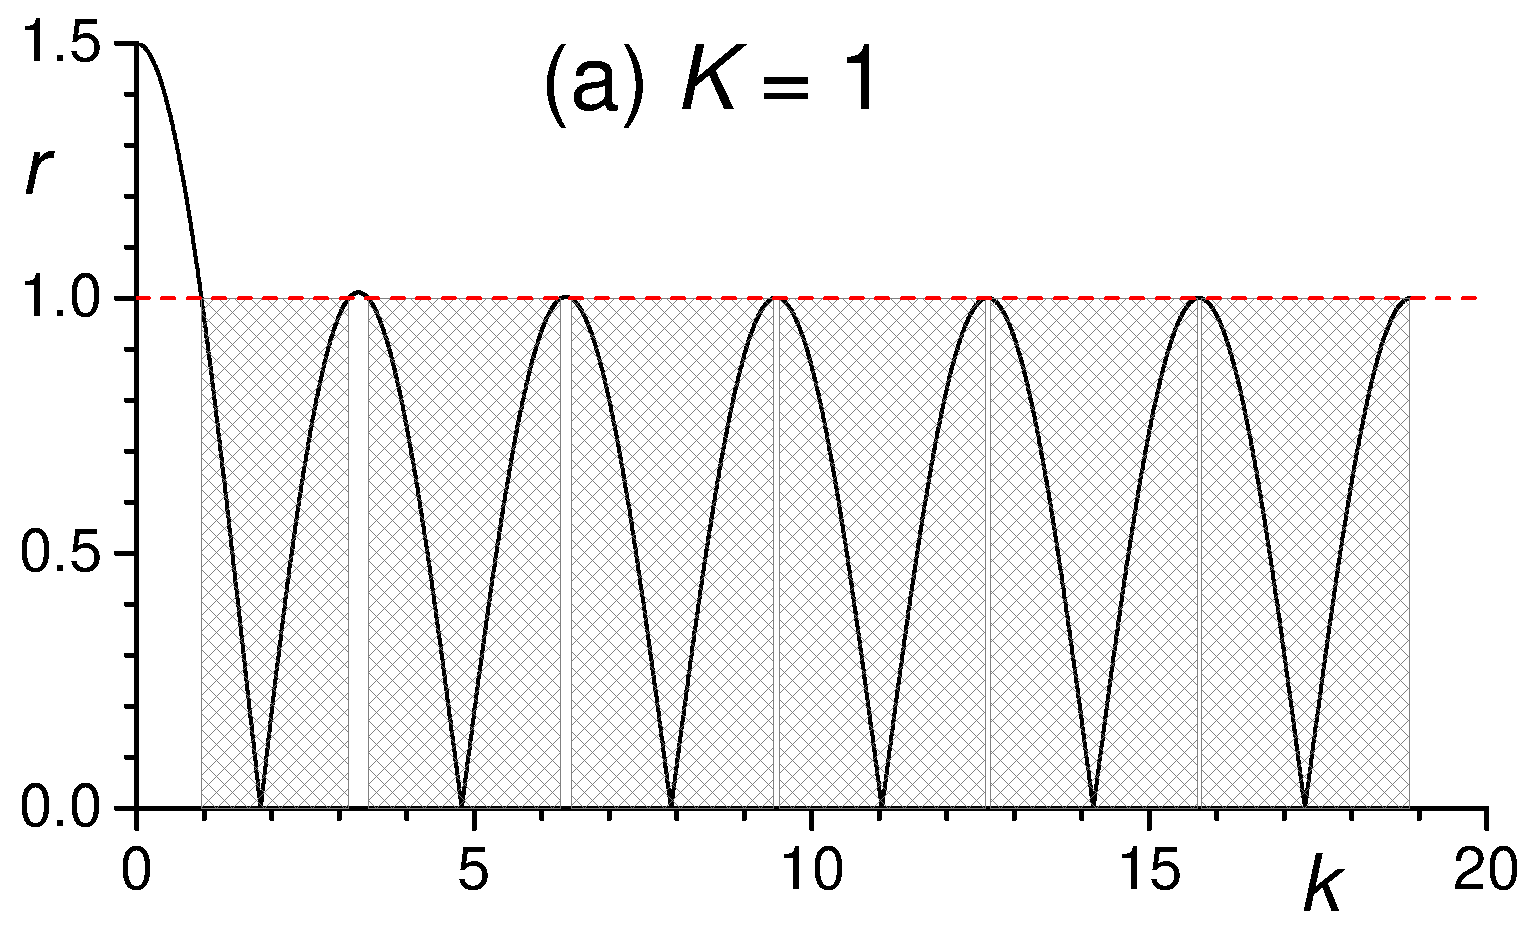
\epsfig{file=bandf1.eps,width=\linewidth}
            \end{subfigure}
            \hfill
            \begin{subfigure}{0.49\linewidth}
                \centering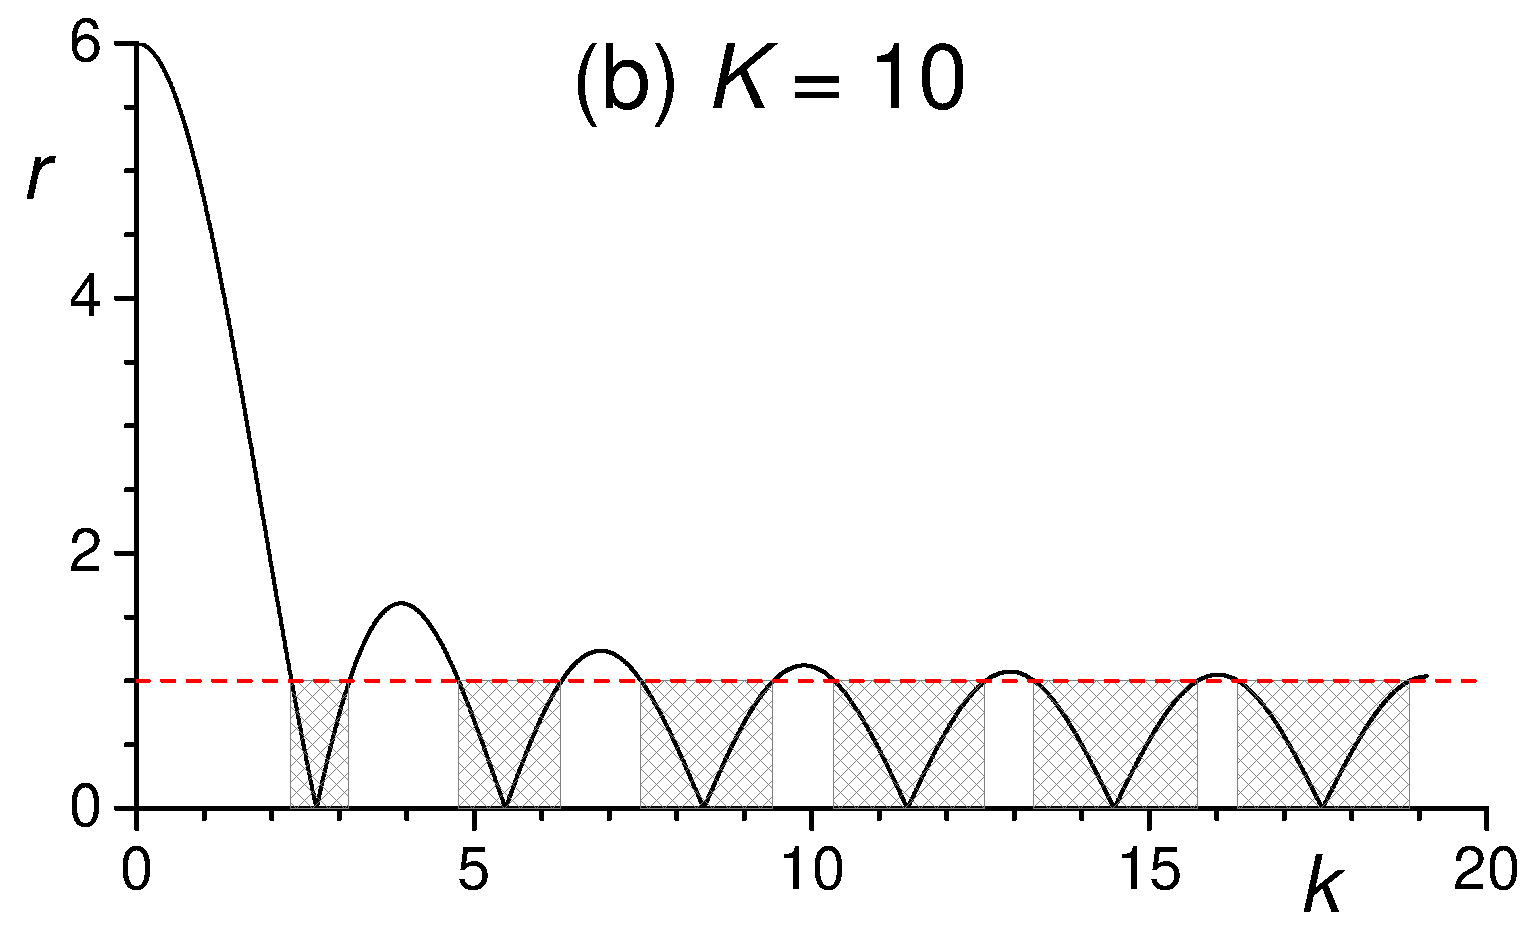
\epsfig{file=bandf10.eps,width=\linewidth}
            \end{subfigure}
			\scaption{
				Funkce $r$ (černá čára) pro dvě hodnoty parametru $K$ a mřížkovou konstantu $a=1$.
				Pásy, v nichž je splněna podmínka~\eqref{eq:DiracCombBandCondition} jsou vyznačeny šrafováním.
			}
			\label{fig:DiracCombBandCondition}
		\end{figure}

		Veličina $r$ je pro dvě hodnoty $K$ zakreslena na obrázku~\ref{fig:DiracCombBandCondition}.
		Několik pozorování:
		\begin{itemize}
		\item
			Pro $K\neq0$ má energetické spektrum ~\emph{pásovou strukturu:} povolené pásy $r\leq1$ střídají zakázané pásy $r>1$, viz obrázek~\ref{fig:DiracCombBandCondition}.
		
		\item
			Hodnota funkce $r$ pro $k=0$ je
			\begin{equation}
				r_{0}=\abs{1+\frac{Ka}{2}},
			\end{equation}
			tj. pokud $K>0$ nebo $K<-\frac{4}{a}$, je na nulové energii vždy zakázaný pás.
			
		\item
			Pro $K>0$ je horní hranice povoleného pásu vždy na hodnotě
			\begin{equation}\label{eq:DiracCombBandTop}
				ka=n\pi,\qquad n\in\mathbb{N}.
			\end{equation}
			Pásy lze tedy indexovat číslem $n$.

		\item
			Pokud $K=0$, jsou povolené všechny energie $E>0$.
			Řešení odpovídá pohybu volné částice.
			
		\item
			S rostoucí hodotou $K$ se pásy zužují a pro $K\rightarrow\infty$ se spektrum redukuje na čárové spektrum~\eqref{eq:DiracCombBandTop}, tj.
			\begin{equation}
				E_{n}=\frac{\hbar^{2}\pi^{2}}{2Ma^{2}}n^{2},
			\end{equation}
			což odpovídá spektru nekonečné hluboké jednorozměrné pravoúhlé jámy šířky $a$.
		\end{itemize}		

	\item
		\begin{figure}[!htbp]
            \begin{subfigure}{0.49\linewidth}
                \centering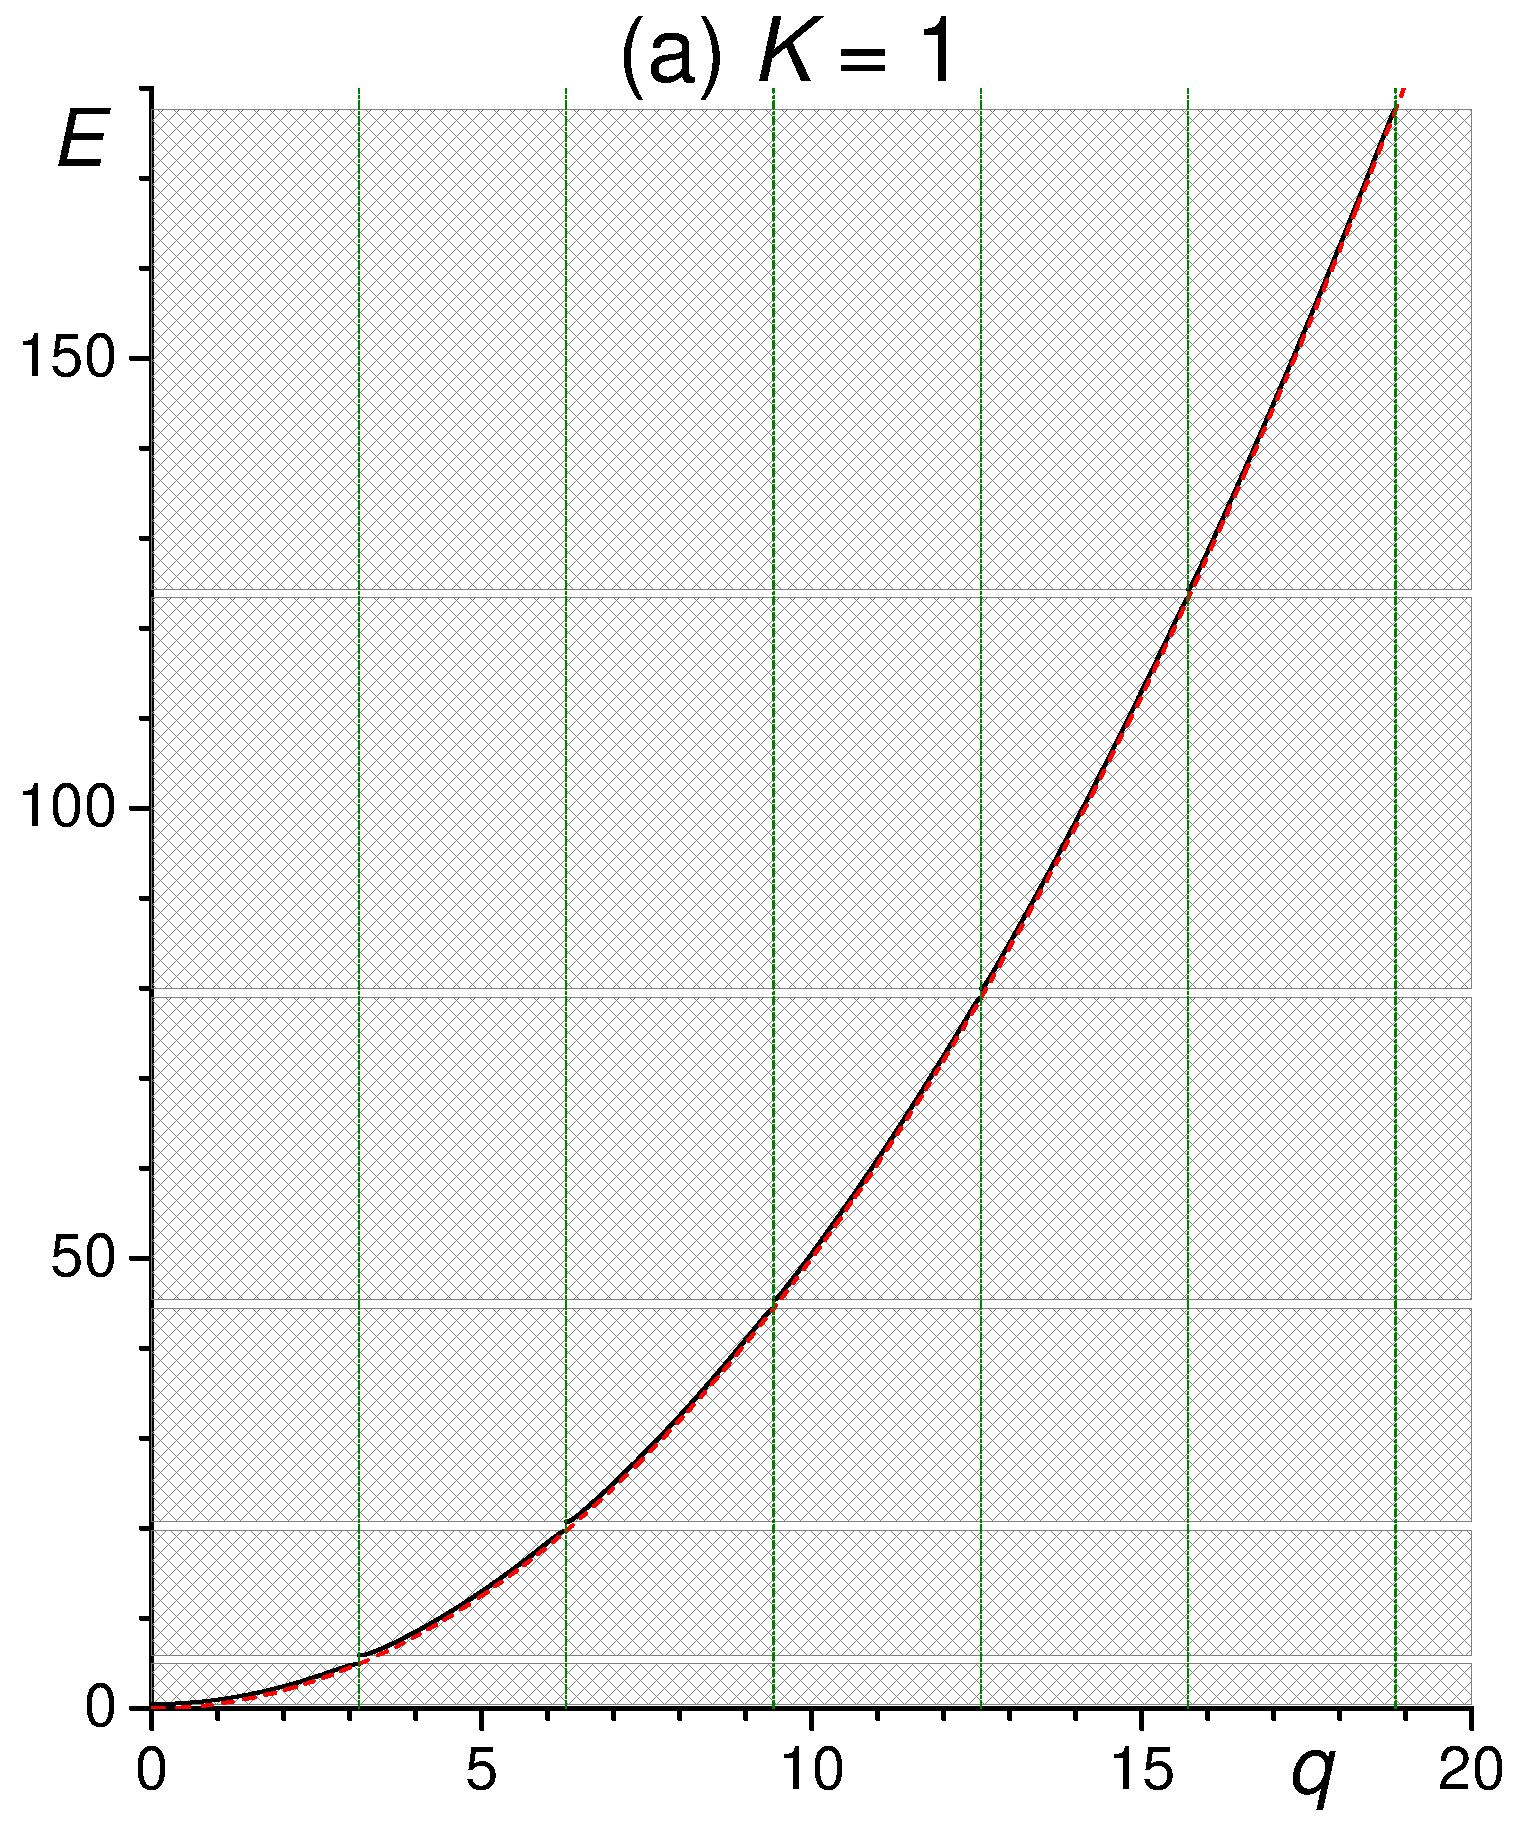
\epsfig{file=bands1.eps,width=\linewidth}
            \end{subfigure}
            \hfill
            \begin{subfigure}{0.49\linewidth}
                \centering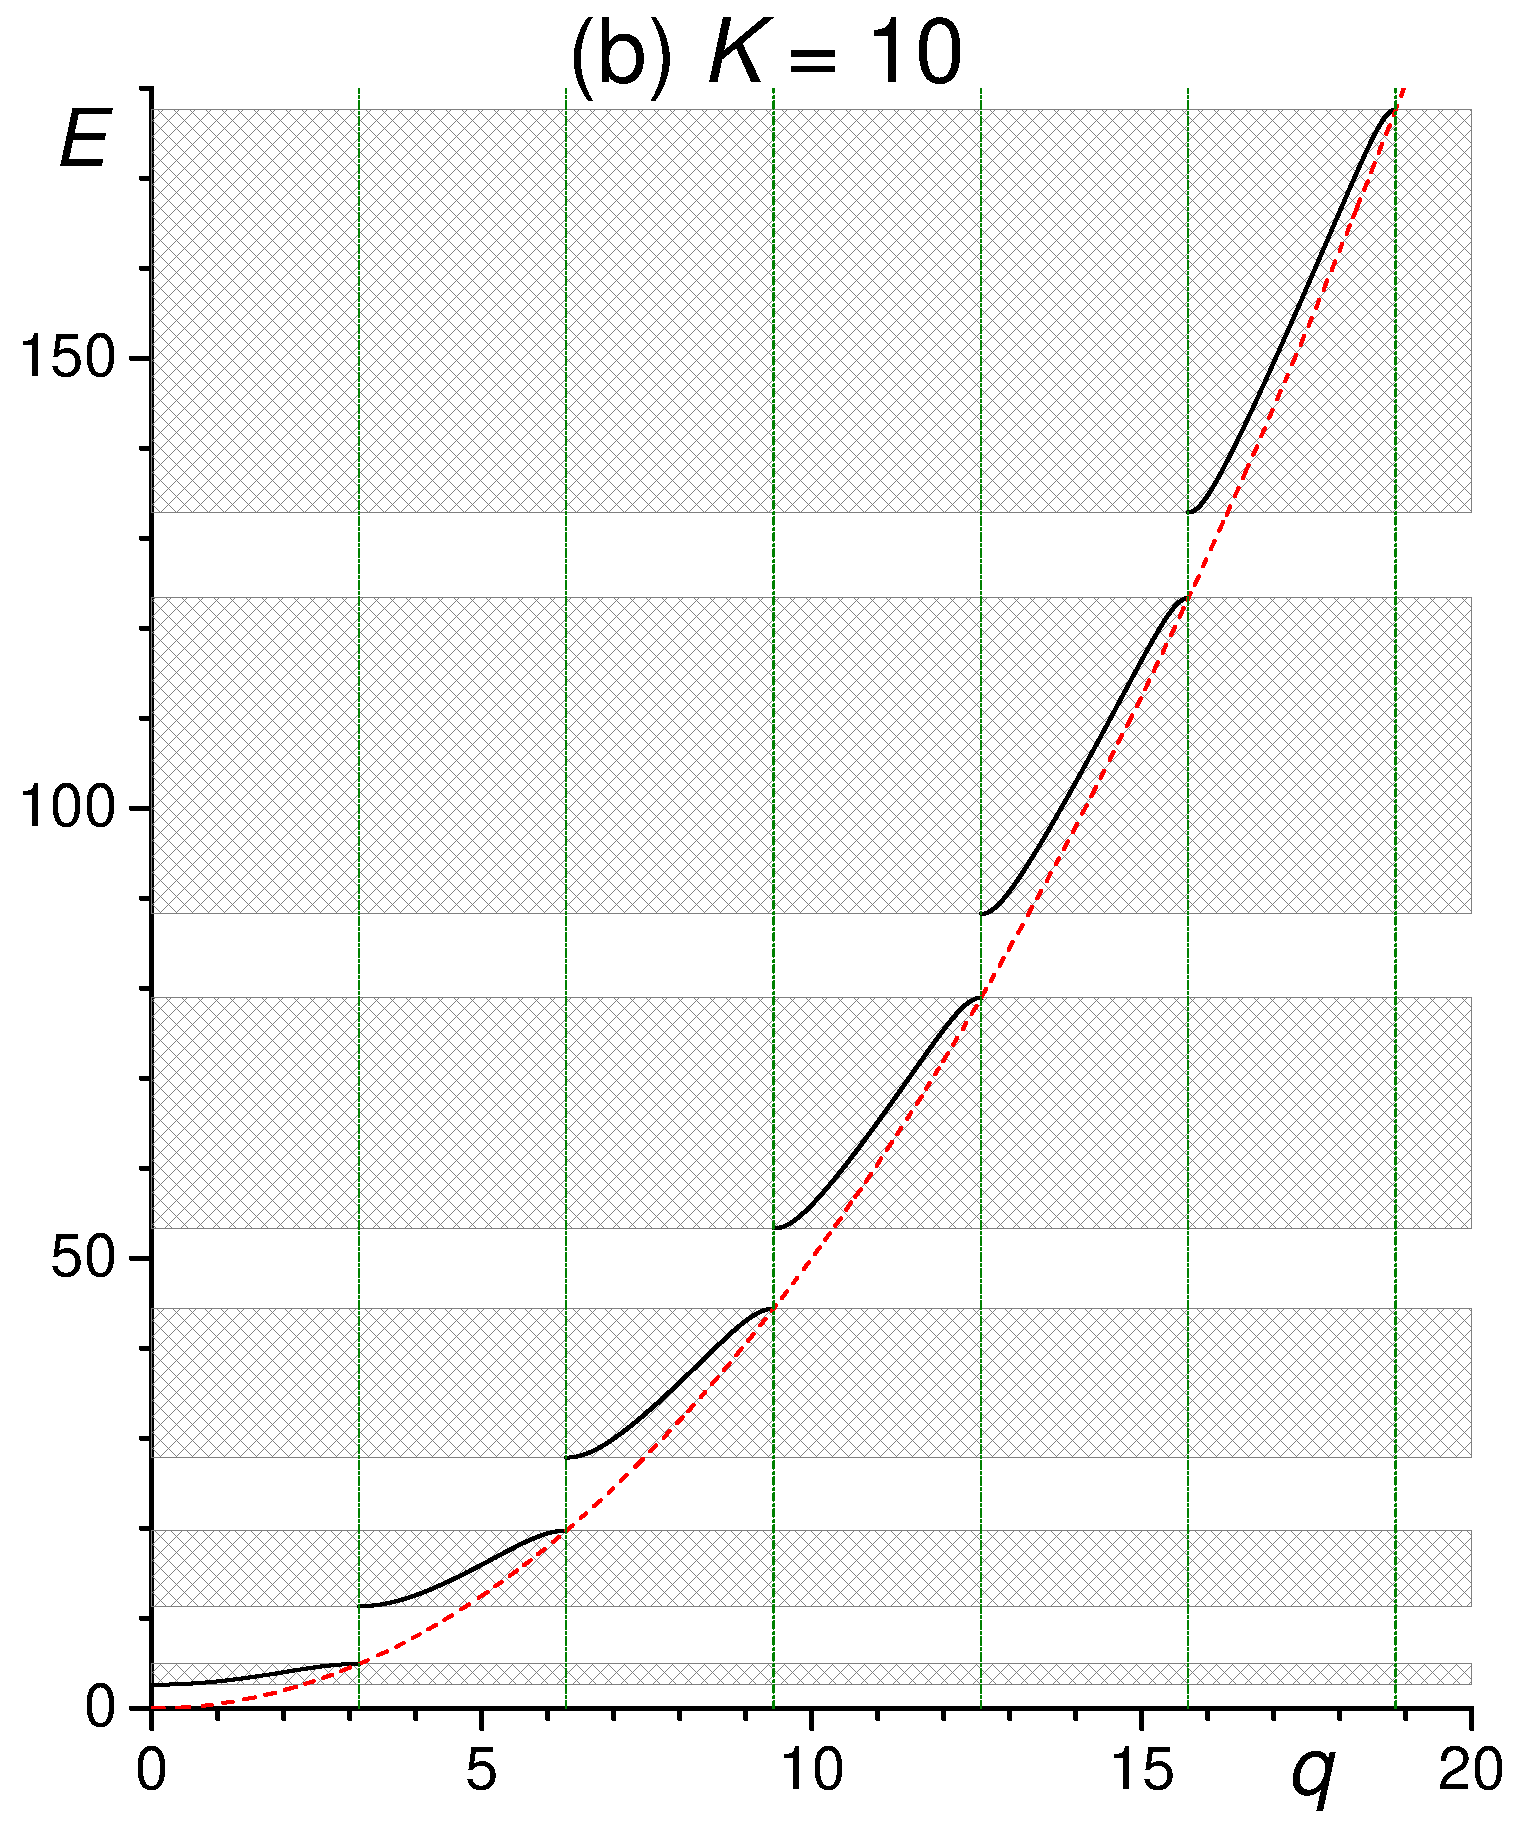
\epsfig{file=bands10.eps,width=\linewidth}
            \end{subfigure}
            \begin{subfigure}{0.49\linewidth}
                \centering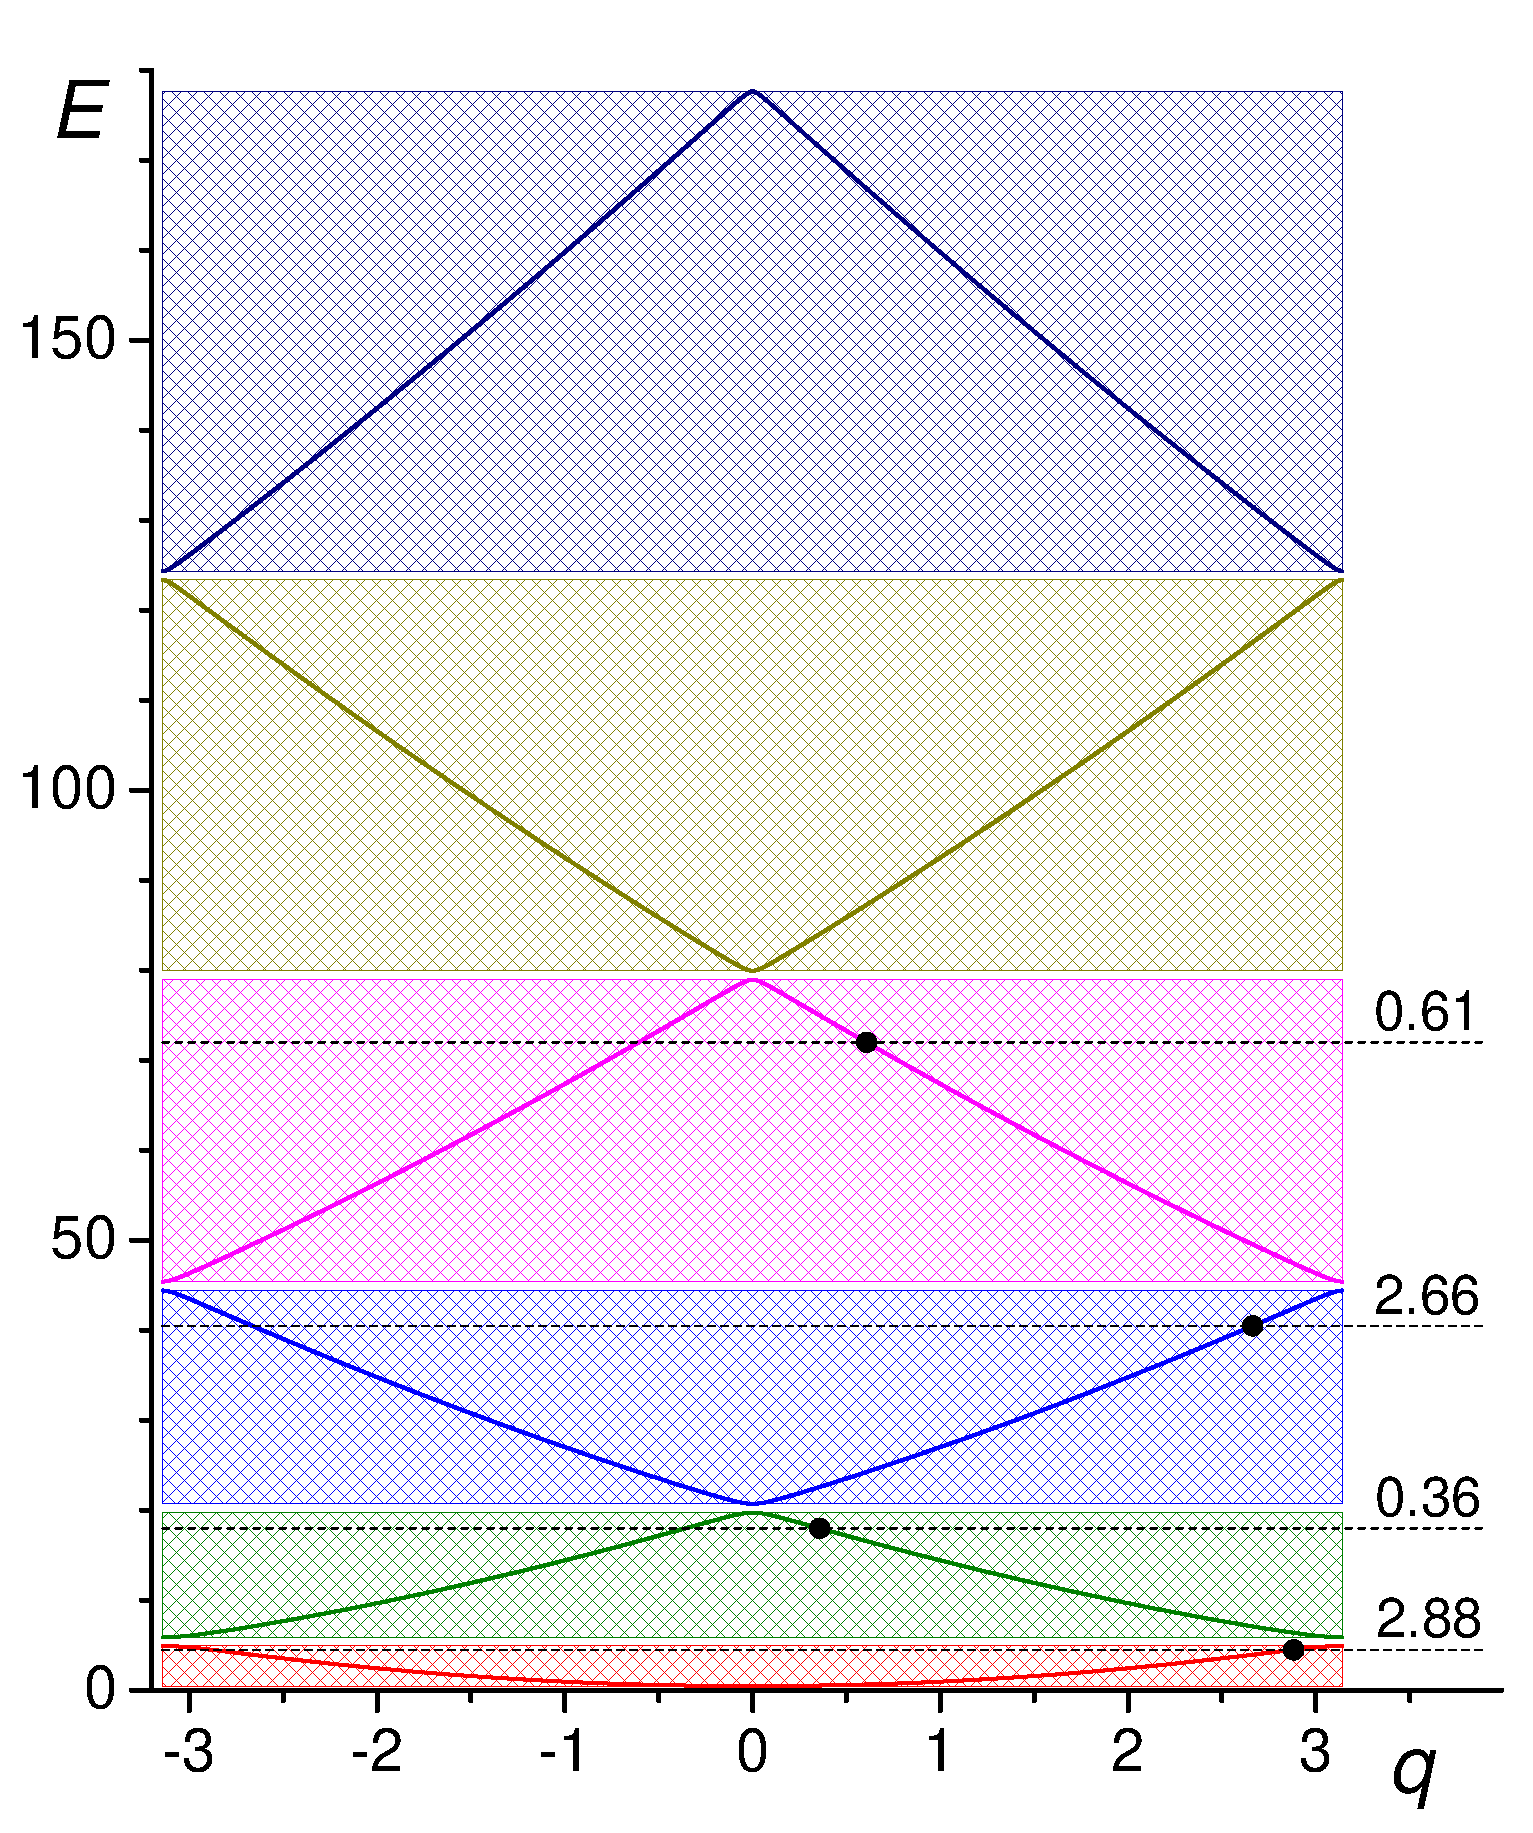
\epsfig{file=Brillouin1.eps,width=\linewidth}
            \end{subfigure}
            \hfill
            \begin{subfigure}{0.49\linewidth}
                \centering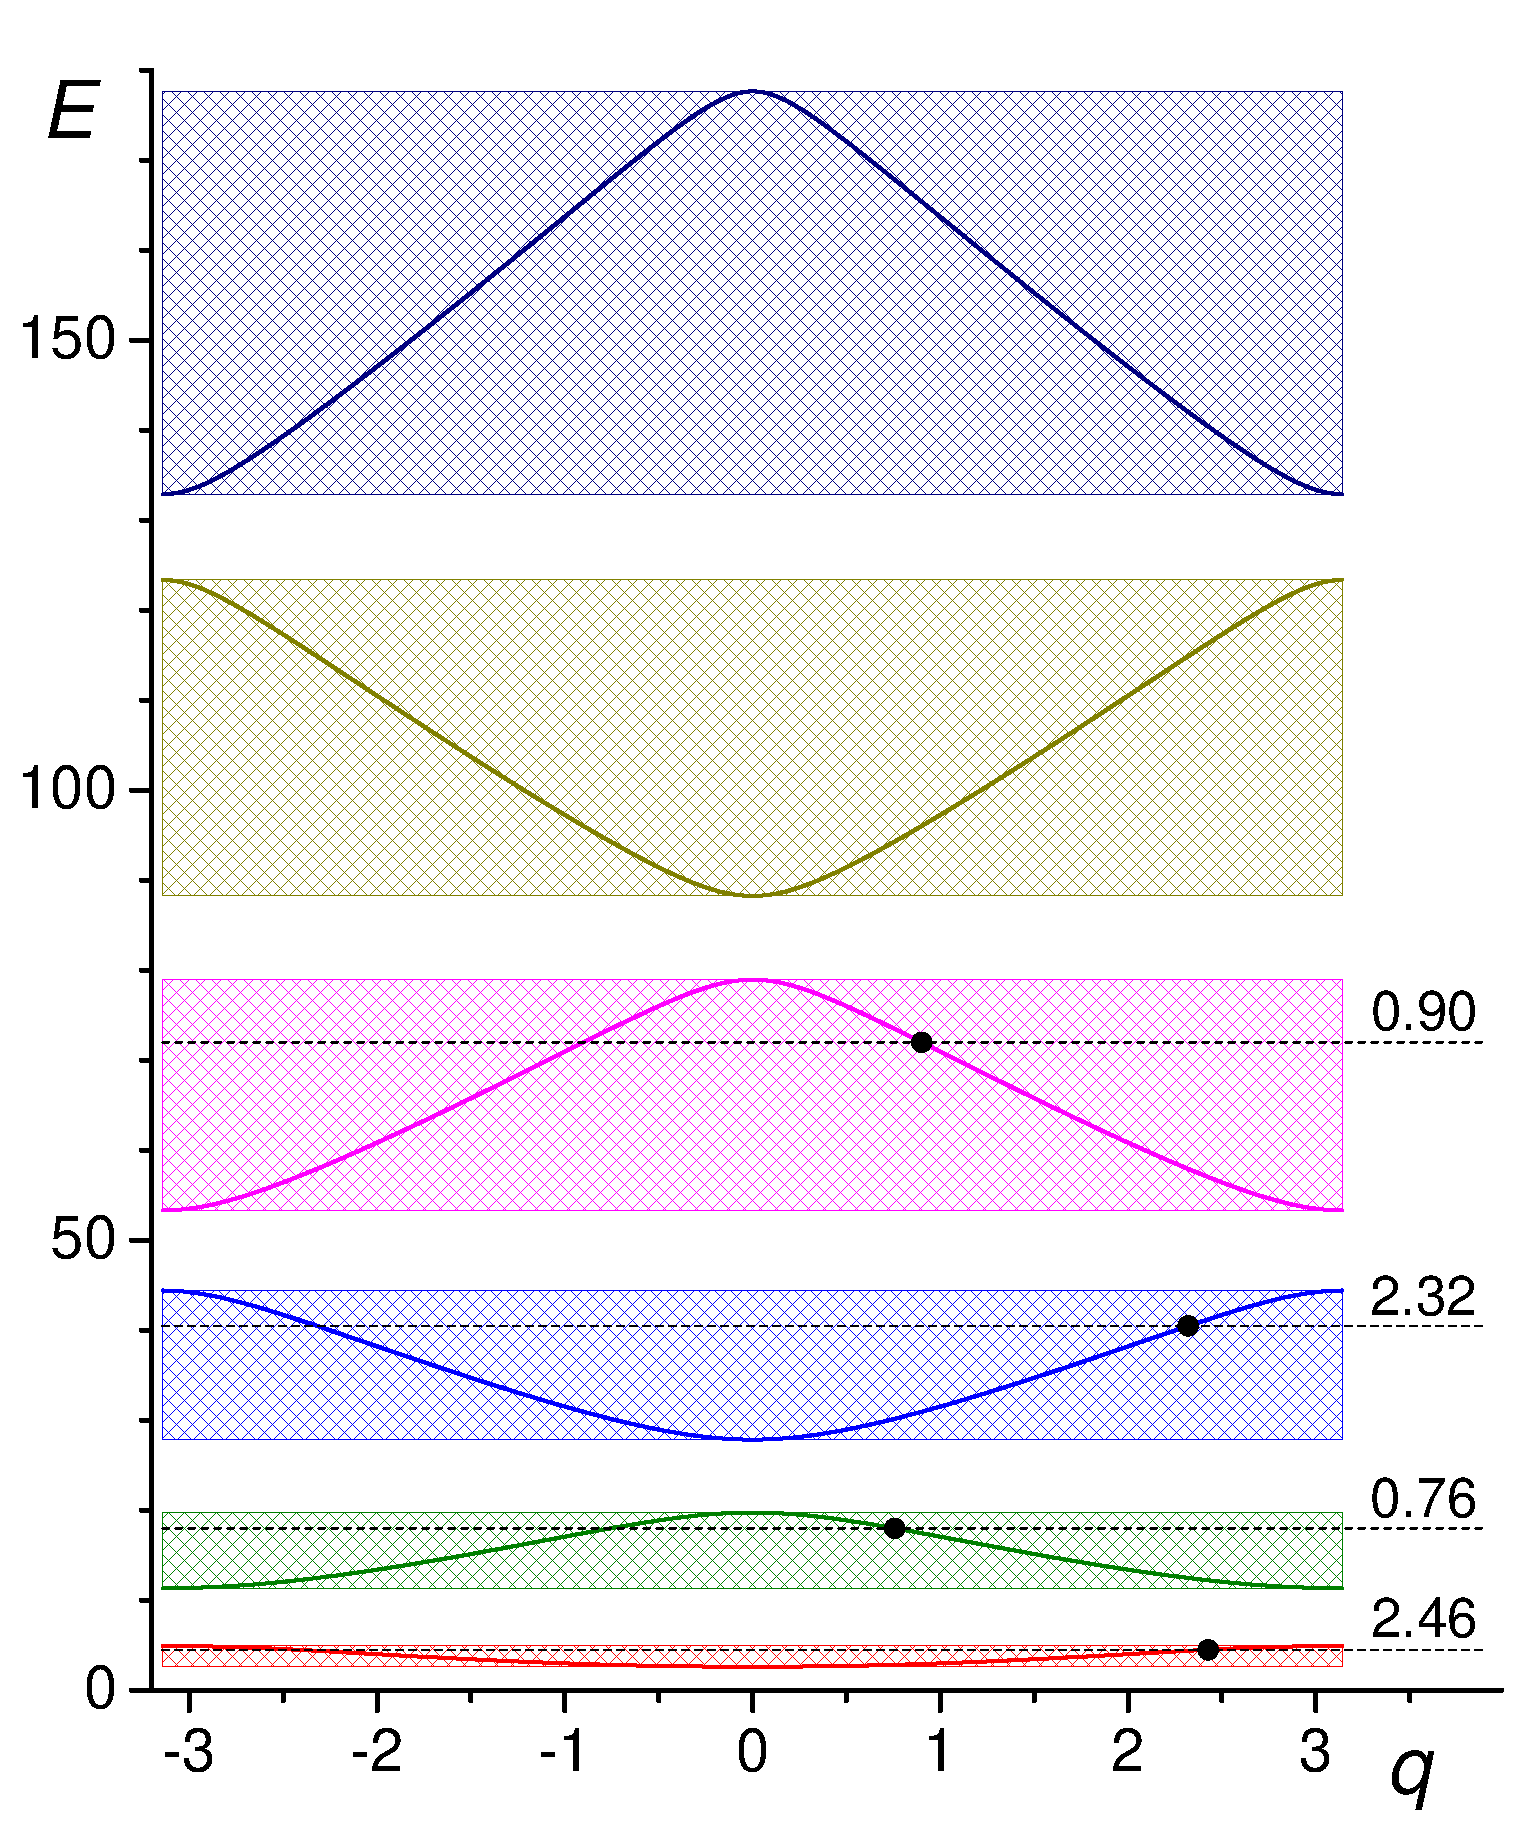
\epsfig{file=Brillouin10.eps,width=\linewidth}
            \end{subfigure}
			\scaption{
				\emph{1. řádek:} Disperzní relace v konvenci~\eqref{eq:DiracCombBandUnique} pro dvě hodnoty $K$ (černá čára).
				Červená čárkovaná čára odpovídá disperzní relaci pro volnou částici $E=\hbar^{2}q^{2}/(2M)$.
				Svislé zelené čerchované čáry vyznačují horní hranice pásů~\eqref{eq:DiracCombBandTop}.				
				Šrafováním jsou znázorněny povolené pásy.				
				\emph{2. řádek:}
				Disperzní relace pro 1. Brillouinovu zónu~\eqref{eq:Brillouin}.
				Jednotlivé pásy jsou znázorněny odlišnými barvami.
				Černými čárkovanými čarami jsou vyznačeny energie a vypsány hodnoty kvazihybnosti $q$ pro obrázek~\ref{fig:DiracCombWaveFunctions}.
			}
			\label{fig:DiracCombBands}
		\end{figure}

		Pokud rovnici~\eqref{eq:DiracCombBand} pro hodnotu $ka$ splňuje nějaké $qa$, pak ji stejně dobře splňuje $qa+2\pi m$, kde $m\in\mathbb{Z}$, přičemž vlnová funkce zůstane stejná.
		Jedna možná konvence znázornění výsledů tedy spočívá v tom, že se ke každé hodnotě $\pi n\leq ka\leq\pi(n+1)$ přidruží $qa$ tak, aby leželo v intervalu $\pi m\leq qa\leq\pi(m+1)$ pro $n=m$, tj.
        \begin{subequations}
            \begin{align}
                &\pi n\leq ka\leq\pi(n+1),\\
                &\pi n\leq qa\leq\pi(n+1),\qquad n\in\mathbb{N}.
            \end{align}
            \label{eq:DiracCombBandUnique}
        \end{subequations}
		Tímto způsobem je docíleno jednoznačného přiřazení $k\leftrightarrow q$.

		Druhá běžně používaná konvence omezuje hodnotu $q$ na tzv. \emph{1. Brillouinovu zónu},\index{zóna!Brillouinova} což je množina nejmenších $q$ takových, že dávají v daném pásu $n$ jednoznačně vlnovou funkci.
		Pro jednorozměrnou mřížku je 1. Brillouinova zóna interval
		\begin{equation}\label{eq:Brillouin}
			qa\in[-\pi,\pi].
		\end{equation}

        Disperzní relace $E=E(q)$ v obou konvencích je zobrazena na obrázku~\ref{fig:DiracCombBands}.
		
		\begin{figure}[!htbp]
            \begin{subfigure}{0.49\linewidth}
                \centering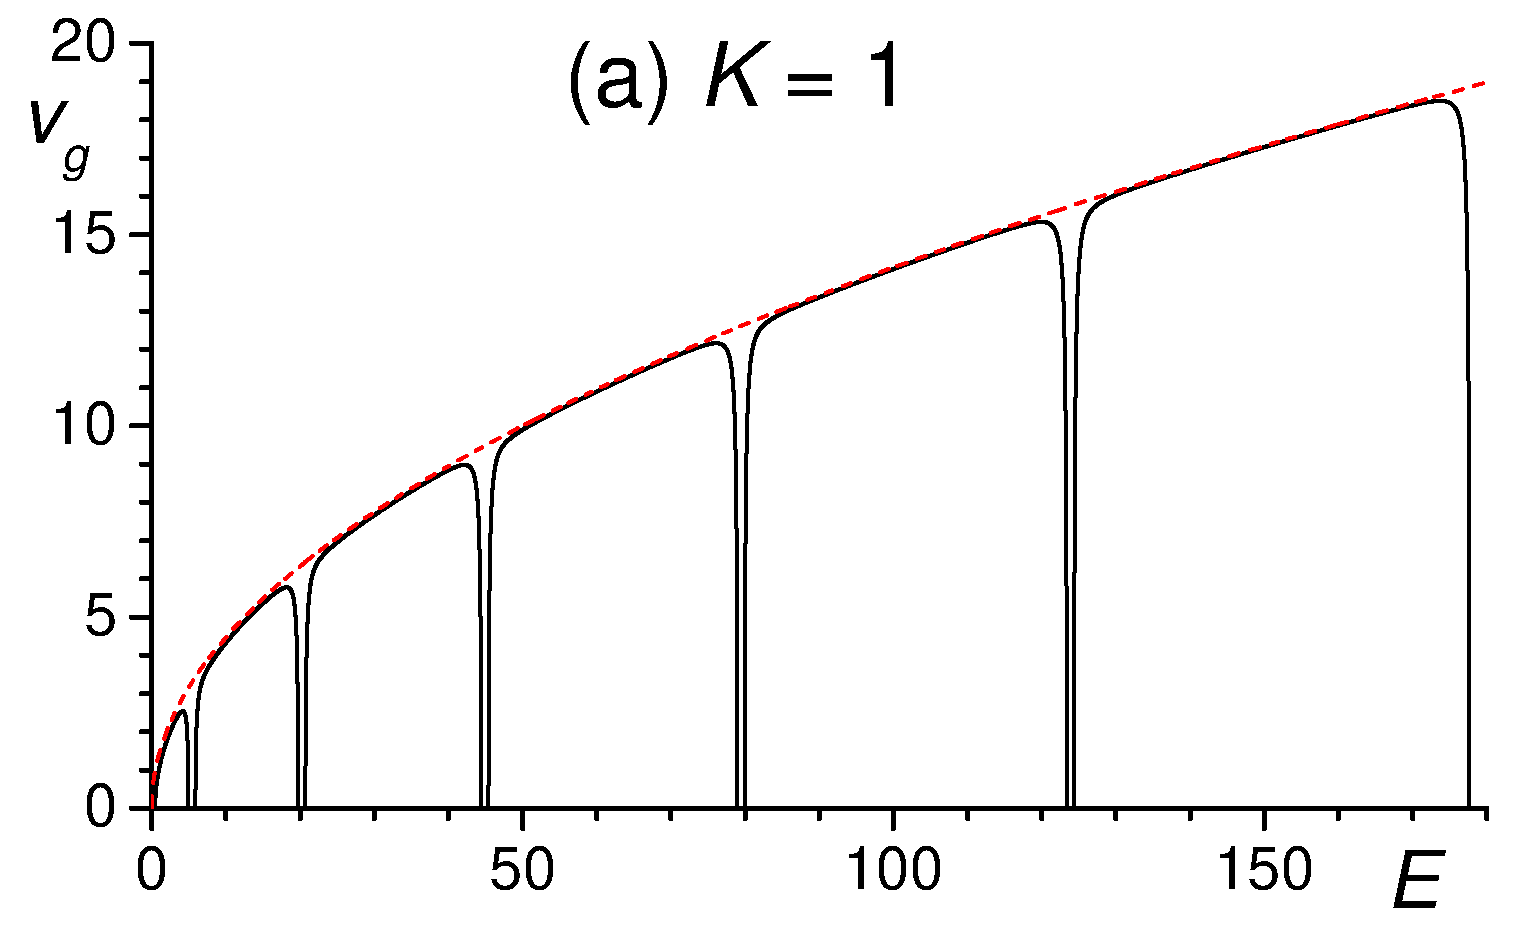
\epsfig{file=vgE1.eps,width=\linewidth}
            \end{subfigure}
            \hfill
            \begin{subfigure}{0.49\linewidth}
                \centering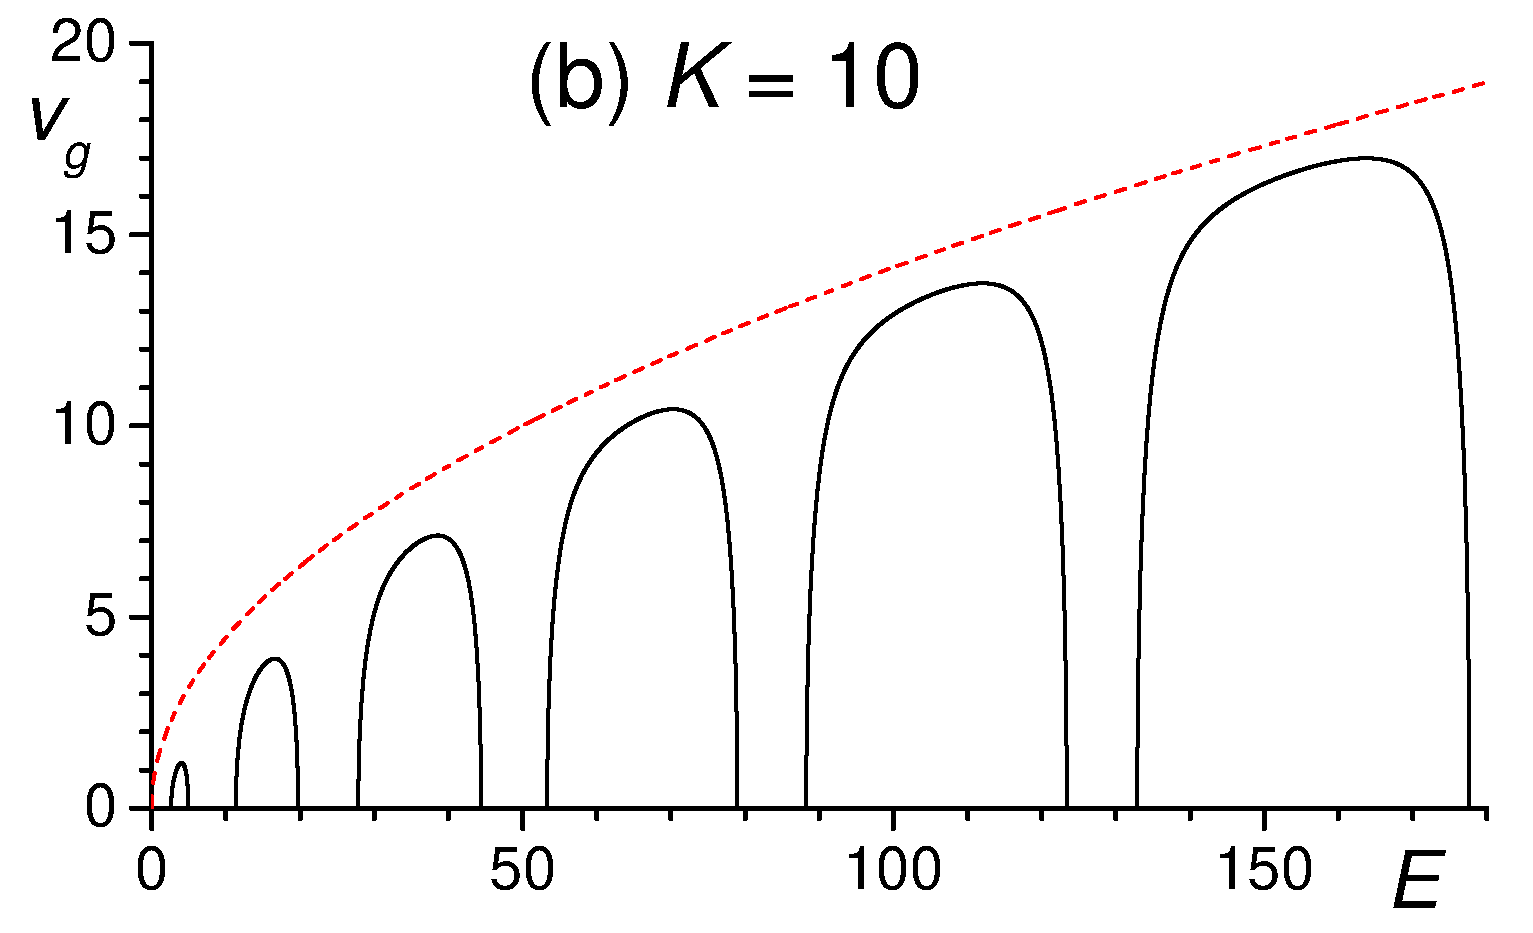
\epsfig{file=vgE10.eps,width=\linewidth}
            \end{subfigure}
            \begin{subfigure}{0.49\linewidth}
                \centering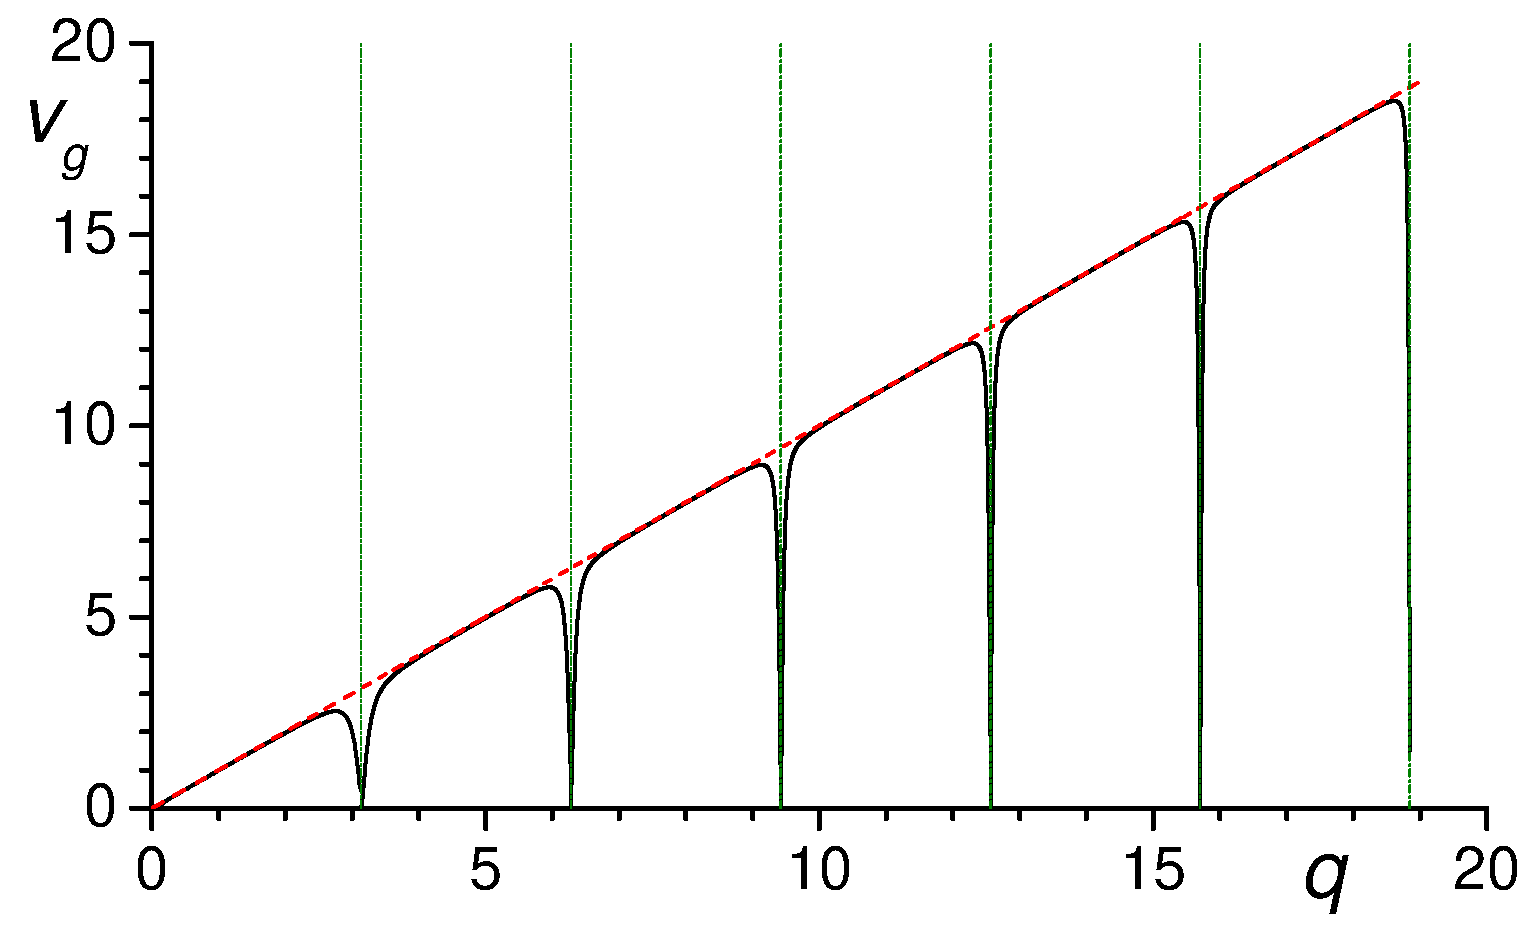
\epsfig{file=vgq1.eps,width=\linewidth}
            \end{subfigure}
            \hfill
            \begin{subfigure}{0.49\linewidth}
                \centering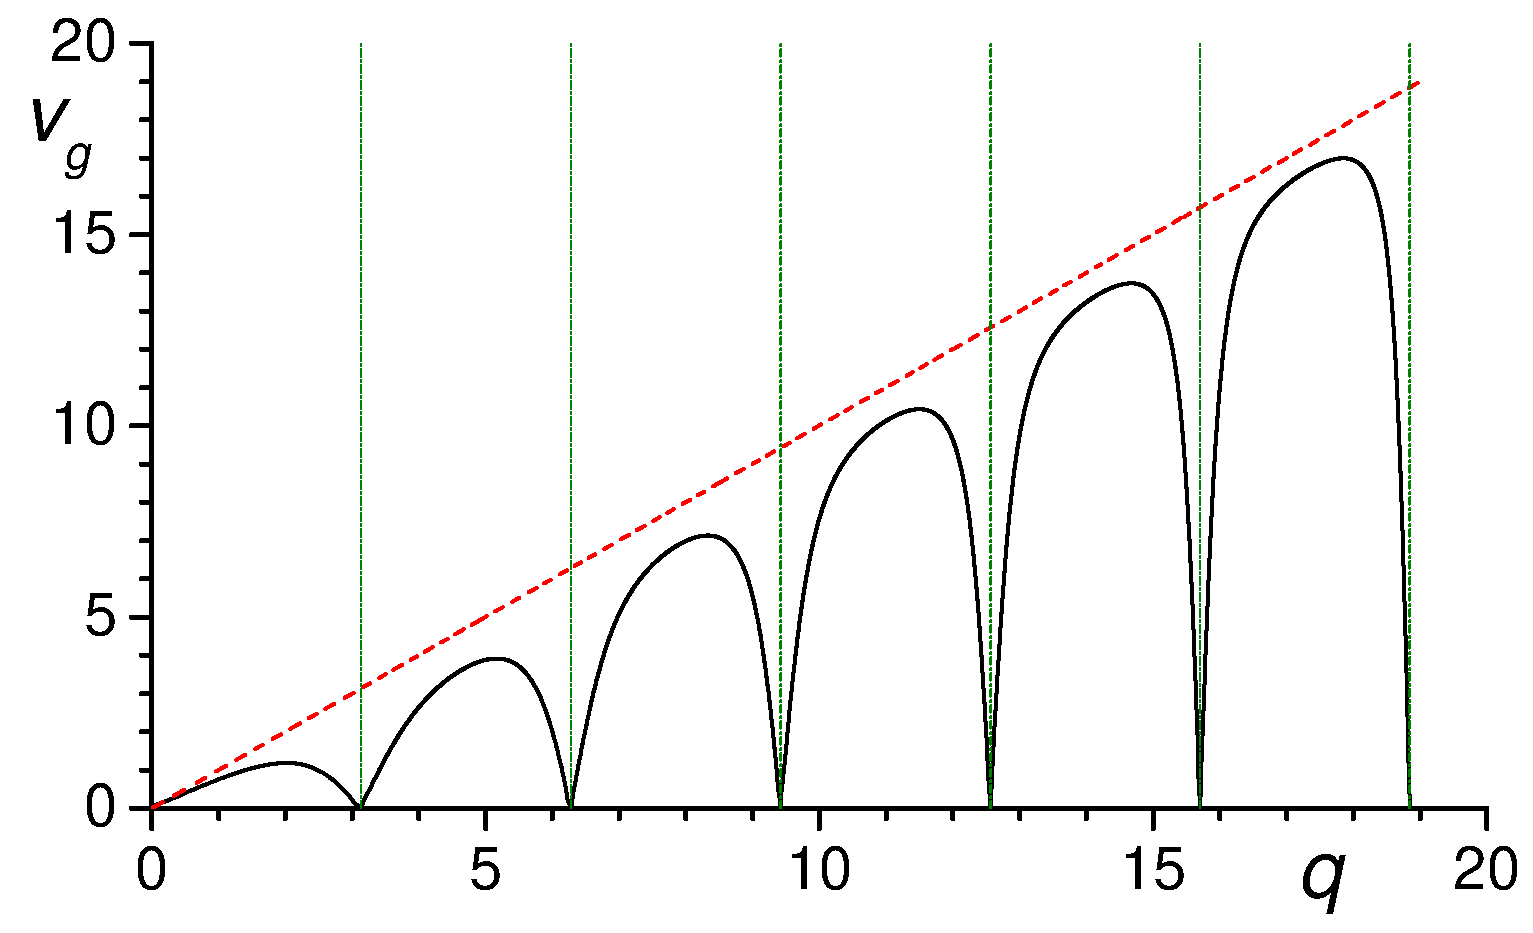
\epsfig{file=vgq10.eps,width=\linewidth}
            \end{subfigure}
			\scaption{
				Grupová rychlost~\eqref{eq:DiracCombGroupVelocity} v závislosti na energii (1. řádek) a na kvazihybnosti (2. řádek).
				Ve 2. řádku jsou hranice pásů $q=\pi n$ znázorněny svislými zelenými čerchovanými čarami.
				Červená čárkovaná čára odpovídá rychosti pro volnou částici $E=\hbar q/M$.
			}
			\label{fig:DiracCombGroupVelocity}
		\end{figure}

        \begin{note}
            V 1. Brillouinově zóně musí mít Schrödingerova rovnice dvě lineárně nezávislá řešení.
            Druhé řešení získáme komplexním sdružením $\psi_{q}(x)\mapsto\psi_{q}^{*}(x)=\psi_{-q}(x)$.
            Tato vlnová funkce odpovídá opačné hodnotě kvazihybnosti.
        \end{note}
    
    \item
		Grupová rychost je zakreslena na obrázku~\ref{fig:DiracCombGroupVelocity}.
		Pro $q$ v blízkosti hranice pásu klesá rychost k nule.						

    \item
        Ze sešívací podmínky na spojitost vlnové funkce~\eqref{eq:DiracCombSew} plyne
        \begin{equation}
            A\left[1-\e^{-\im q a}\e^{\im k a}\right]=-B\left[1-\e^{-\im q a}\e^{-\im k a}\right],
        \end{equation}
        což dává vztah mezi konstantami $A$ a $B$:
        \begin{subequations}
            \begin{align}
                A&=-B\,\frac{1-\e^{-\im q a}\e^{-\im k a}}{1-\e^{-\im q a}\e^{\im k a}}
                =B\,\frac{\cos{qa}-\cos{ka}}{1-\cos{(q-k)a}}\e^{-\im k a},\\
                B&=-A\,\frac{1-\e^{-\im q a}\e^{\im k a}}{1-\e^{-\im q a}\e^{-\im k a}}
                =B\,\frac{\cos{qa}-\cos{ka}}{1-\cos{(q+k)a}}\e^{\im k a}.
            \end{align}
        \end{subequations}

        Integrace vlnové funkce na intervalu $[0,a]$~\eqref{eq:DiracCombWaveFunctionNormalization} dá podmínku
        \begin{align}
            1&=\int_{0}^{a}\left(A\e^{\im kx}+B\e^{-\im kx}\right)\left(A^{*}\e^{-\im kx}+B^{*}\e^{\im kx}\right)\d x\nonumber\\
             &=\int_{0}^{a}\left(\abs{A}^{2}+\abs{B}^{2}+AB^{*}\e^{2\im kx}+A^{*}B\e^{-2\im kx}\right)\d x\nonumber\\
             &=\left(\abs{A}^{2}+\abs{B}^{2}\right)a+\frac{1}{2\im k}\left[AB^{*}\left(\e^{2\im ka}-1\right)+A^{*}B\left(1-\e^{-2\im ka}\right)\right].
        \end{align}
        Spojení posledních dvou vztahů vede k výrazům
        \begin{align}
            1&=a\abs{B}^{2}\bigg\{1+\left[\frac{\cos{qa}-\cos{ka}}{1-\cos{(q-k)a}}\right]^{2}
                +\underbrace{\frac{2\sin{ka}}{ka}}_{\frac{4}{Ka}\left(\cos{qa}-\cos{ka}\right)}\frac{\cos{qa}-\cos{ka}}{1-\cos{(q-k)a}}\bigg\}\nonumber\\
             &=2a\abs{B}^{2}\frac{1-\cos{qa}\cos{ka}+\frac{2}{Ka}\left(\cos{qa}-\cos{ka}\right)^{2}}{1-\cos{(q-k)a}},
        \end{align}
        kde bylo využito vztahu~\eqref{eq:DiracCombBand} a první dva členy byly upraveny podle vzorců pro goniometrické funkce:
        \begin{align}
            1+\left[\frac{\cos{qa}-\cos{ka}}{1-\cos{(q-k)a}}\right]^{2}
                &=1+\left[\frac{-2\sin{\frac{q-k}{2}a}\,\sin{\frac{q+k}{2}a}}{2\sin^{2}\frac{q-k}{2}a}\right]^{2}\nonumber\\
                &=\frac{\sin^{2}{\frac{q-k}{2}a}+\sin^{2}{\frac{q+k}{2}a}}{\sin^{2}{\frac{q-k}{2}a}}\nonumber\\
                &=\frac{1-\cos{(q-k)a}+1-\cos{(q+k)a}}{1-\cos{(q-k)a}}\nonumber\\
                &=\frac{2-2\cos{qa}\cos{ka}}{1-\cos{(q-k)a}}.
        \end{align}
        
        \begin{figure}[!htbp]
            \begin{subfigure}{0.49\linewidth}
                \centering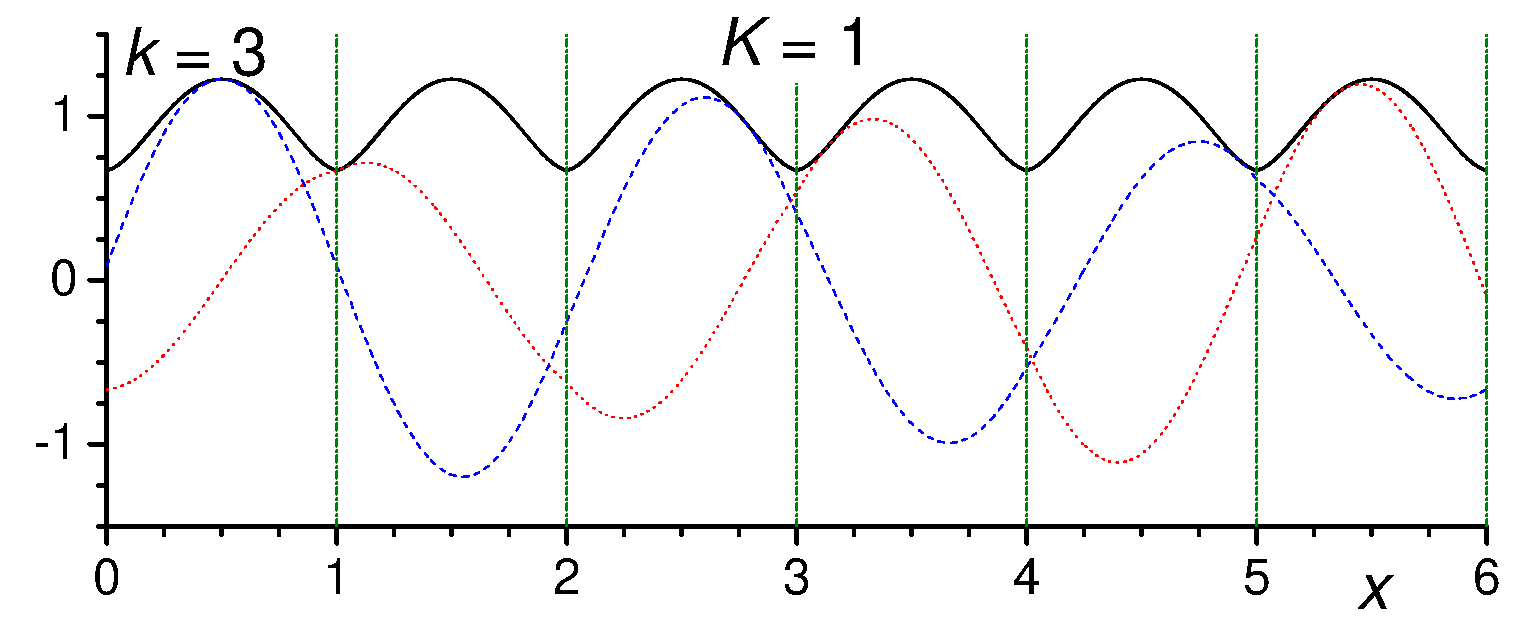
\epsfig{file=psi1_3.eps,width=\linewidth}
            \end{subfigure}
            \hfill
            \begin{subfigure}{0.49\linewidth}
                \centering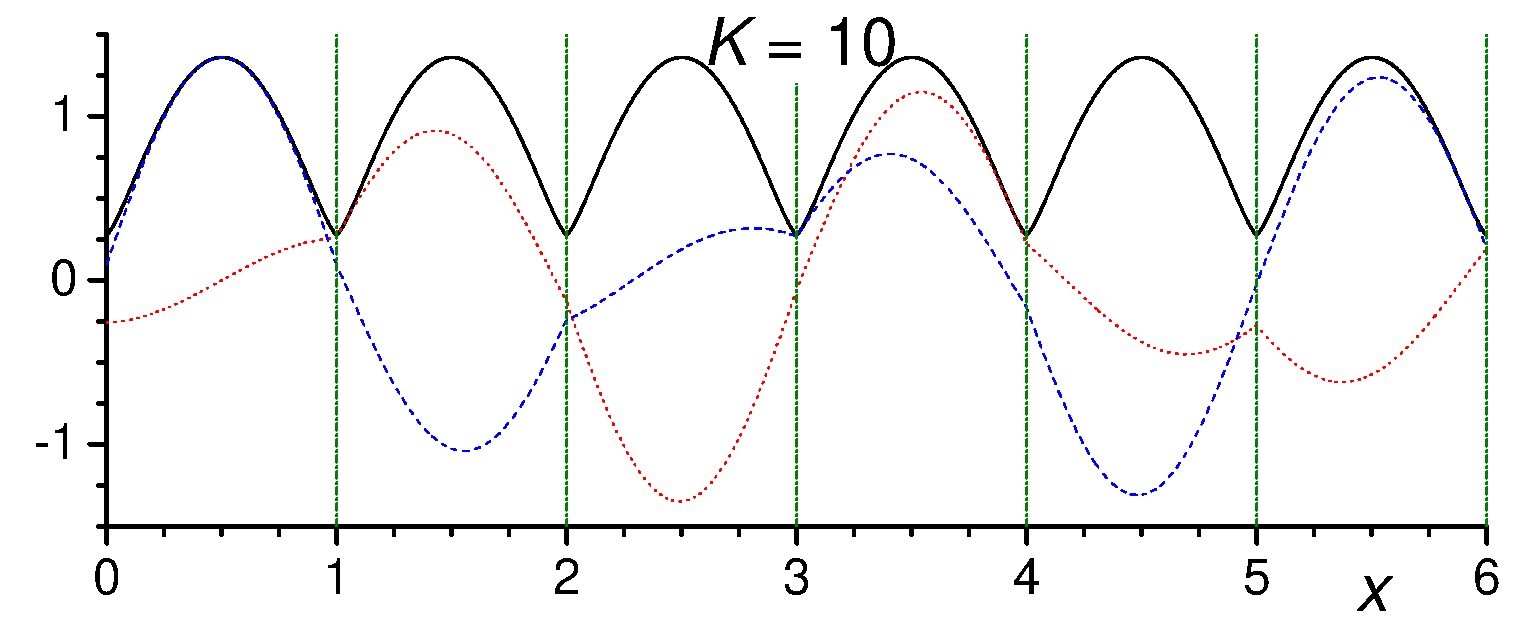
\epsfig{file=psi10_3.eps,width=\linewidth}
            \end{subfigure}
            \begin{subfigure}{0.49\linewidth}
                \centering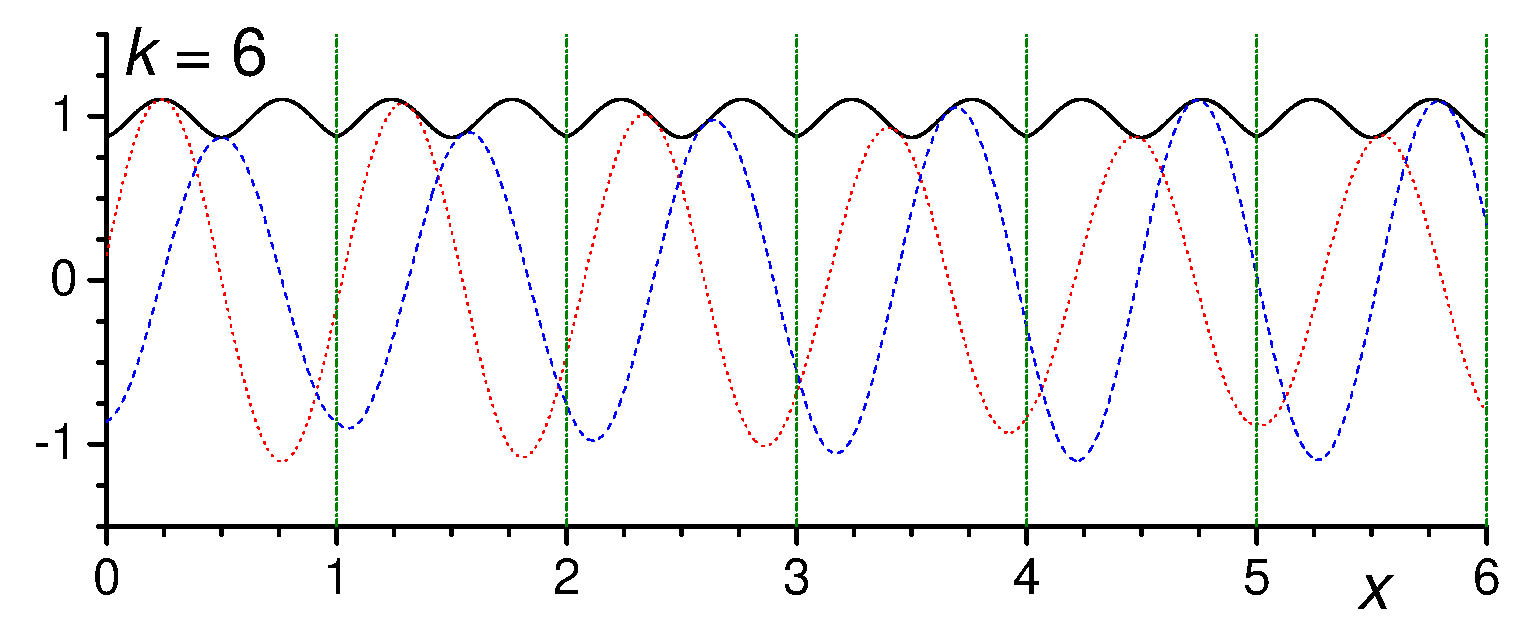
\epsfig{file=psi1_6.eps,width=\linewidth}
            \end{subfigure}
            \hfill
            \begin{subfigure}{0.49\linewidth}
                \centering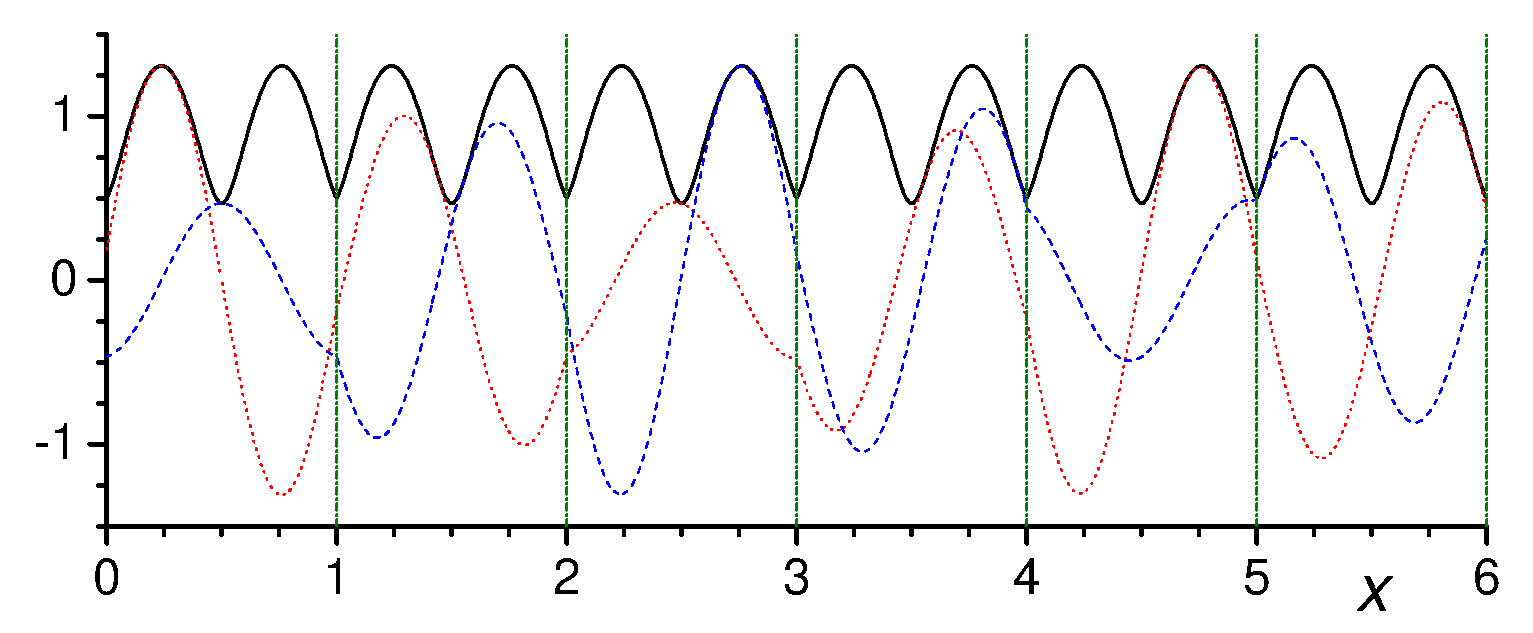
\epsfig{file=psi10_6.eps,width=\linewidth}
            \end{subfigure}
            \begin{subfigure}{0.49\linewidth}
                \centering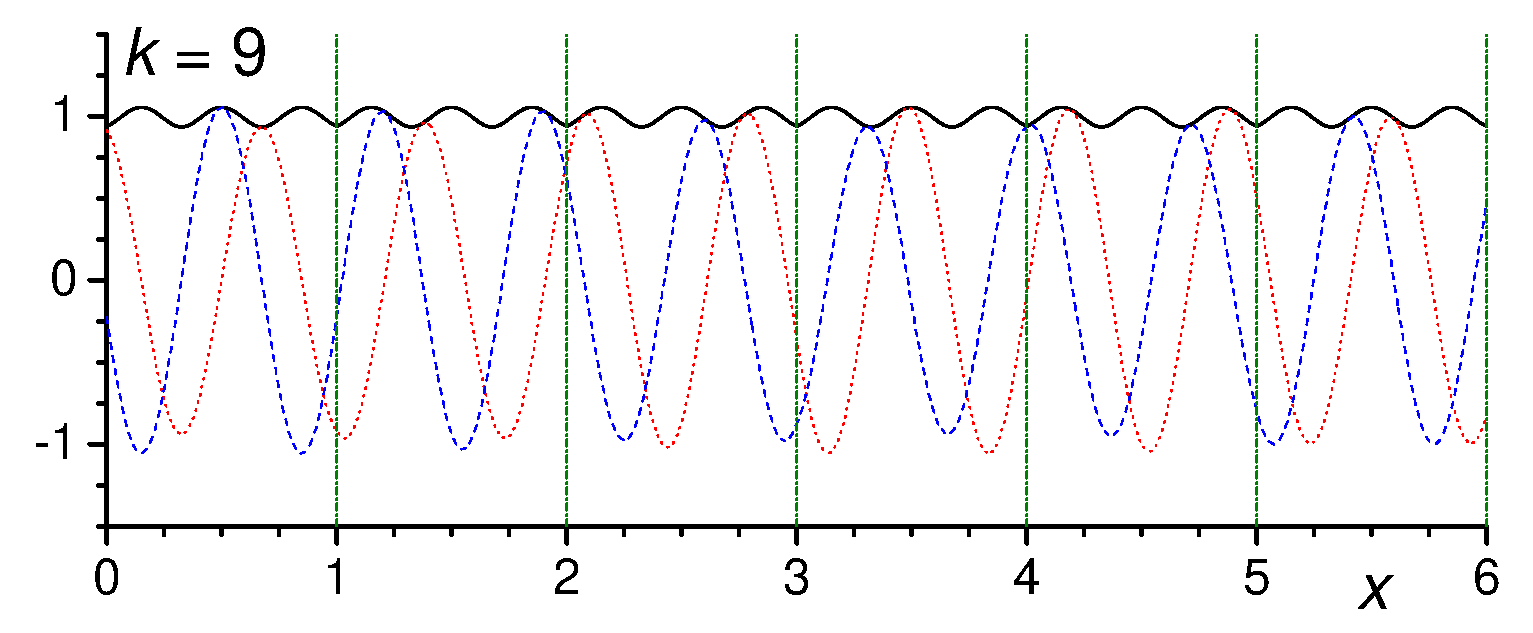
\epsfig{file=psi1_9.eps,width=\linewidth}
            \end{subfigure}
            \hfill
            \begin{subfigure}{0.49\linewidth}
                \centering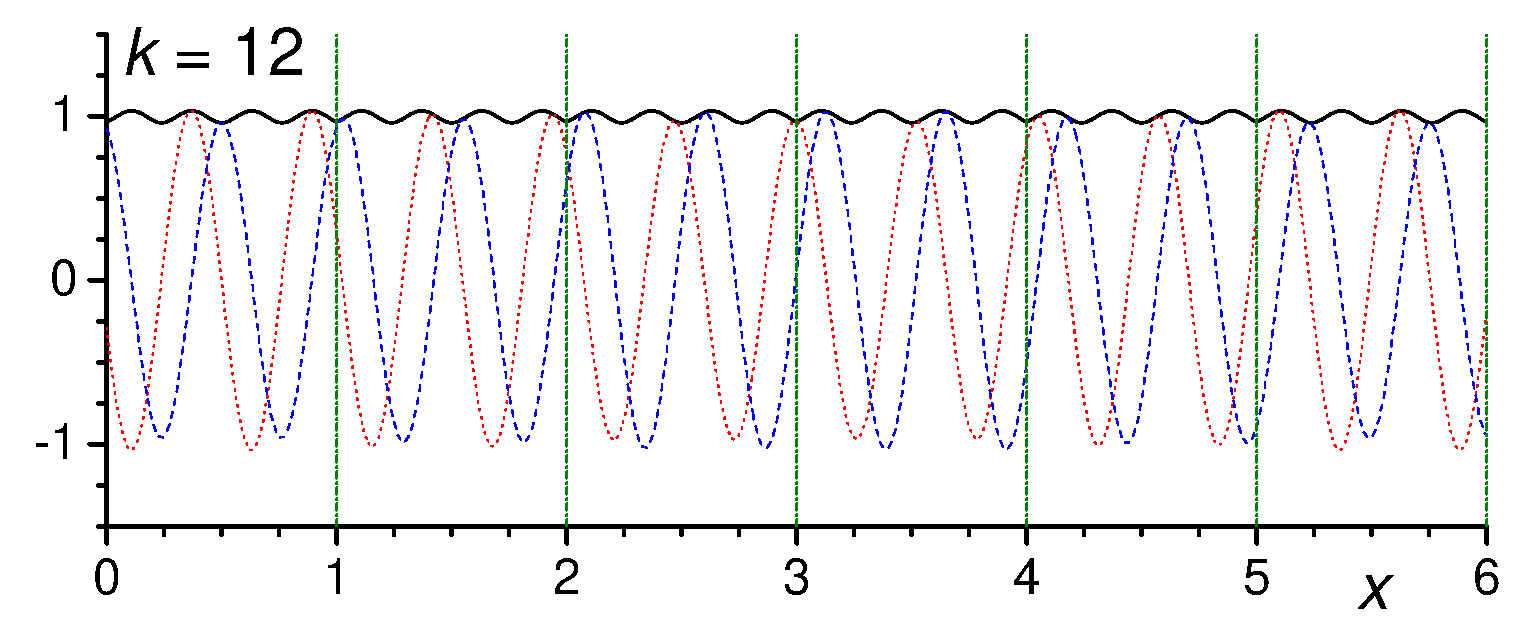
\epsfig{file=psi1_12.eps,width=\linewidth}
            \end{subfigure}
            \begin{subfigure}{0.49\linewidth}
                \centering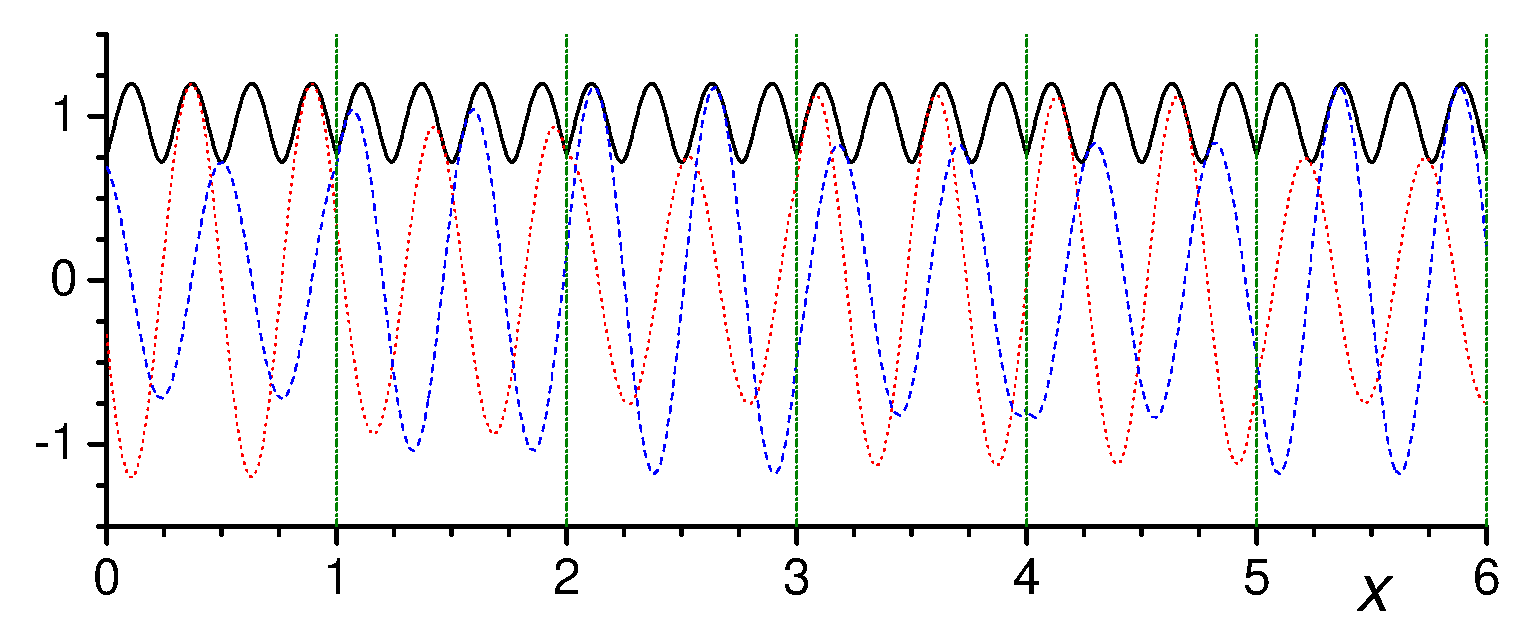
\epsfig{file=psi10_12.eps,width=\linewidth}
            \end{subfigure}
            \hfill
            \begin{subfigure}{0.49\linewidth}
                \centering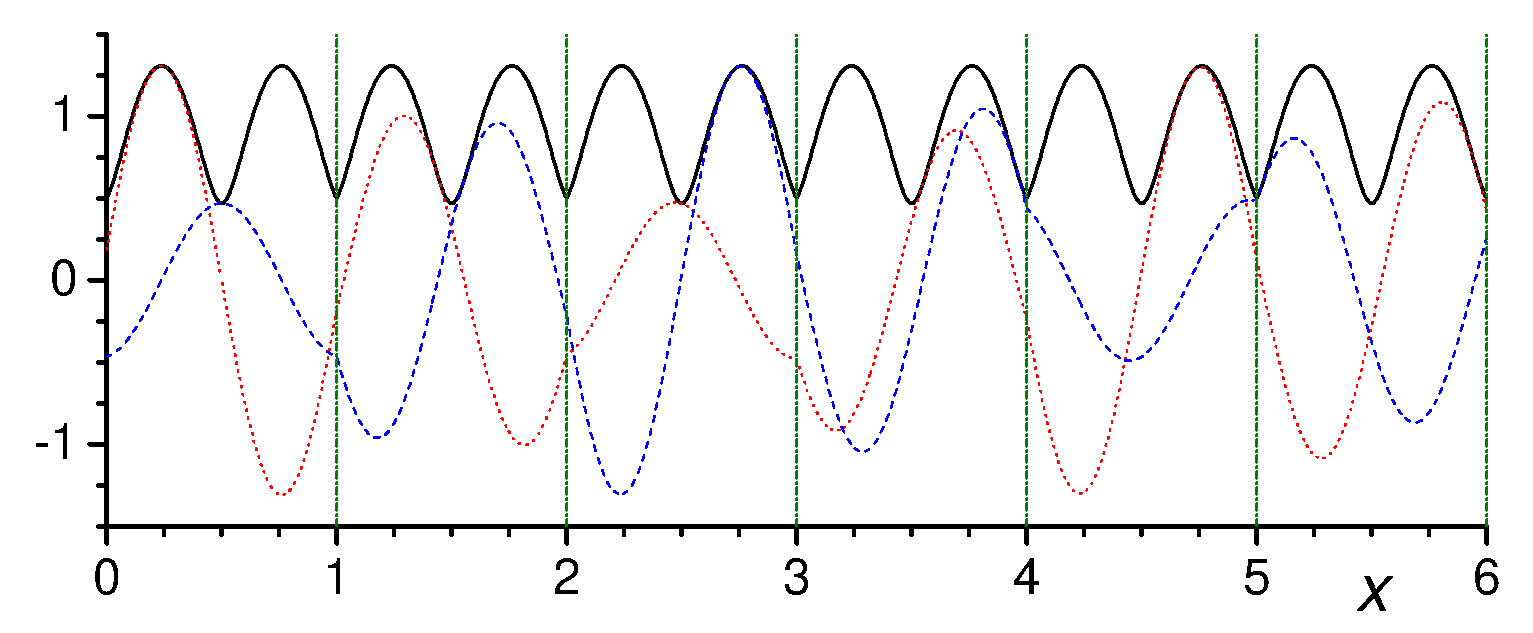
\epsfig{file=psi10_6.eps,width=\linewidth}
            \end{subfigure}
            \scaption{
                Vlnové funkce $\psi_{q}(x)$ normalizované na intervalu $(0,a)$ pro $a=1$, dvě hodnoty $K$ a nejnižší čtyři povolené pásy. 
                Hodnoty $q>0$ leží v 1. Brillouinově zóně.
                Modrá čárkovaná čára -- reálná část, červená tečkovaná čára -- imaginární část, černá čára -- absolutní hodnota.
                Zelené čerchované čáry odpovídají místům, v nichž leží $\delta$-funkce potenciálu.
                Odpovídající energie a hodnoty kvazihybnosti $q$ jsou vyznačeny v obrázku~\ref{fig:DiracCombBands}.
            }
            \label{fig:DiracCombWaveFunctions}
        \end{figure}

        \begin{figure}[!htbp]
            \begin{subfigure}{0.49\linewidth}
                \centering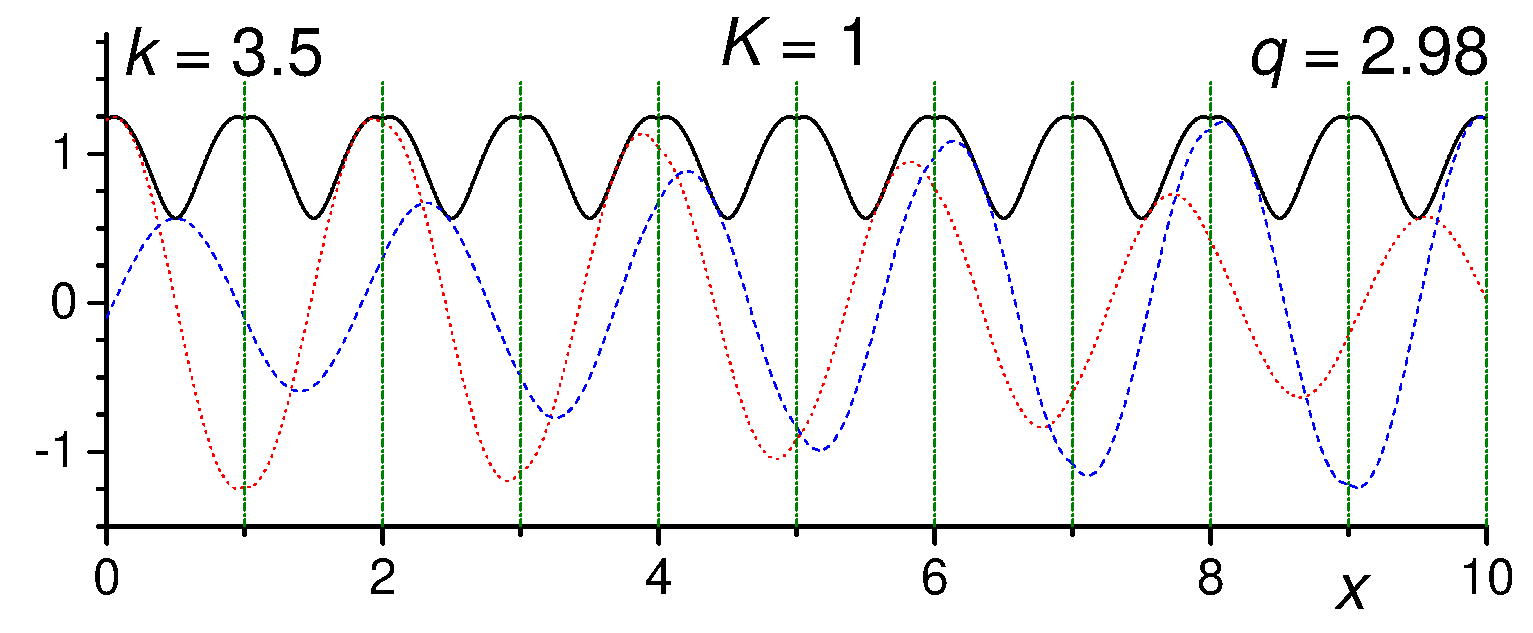
\epsfig{file=psi1s.eps,width=\linewidth}
            \end{subfigure}
            \hfill
            \begin{subfigure}{0.49\linewidth}
                \centering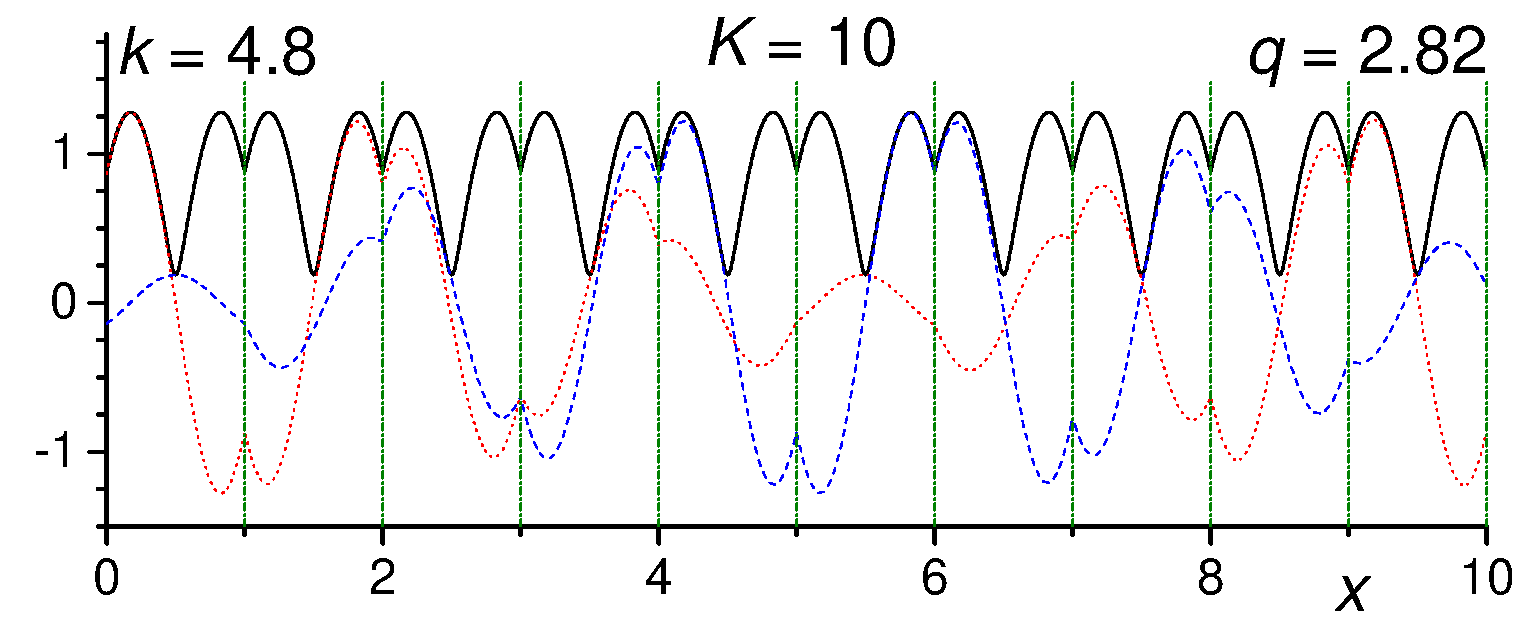
\epsfig{file=psi10s.eps,width=\linewidth}
            \end{subfigure}
            \begin{subfigure}{0.49\linewidth}
                \centering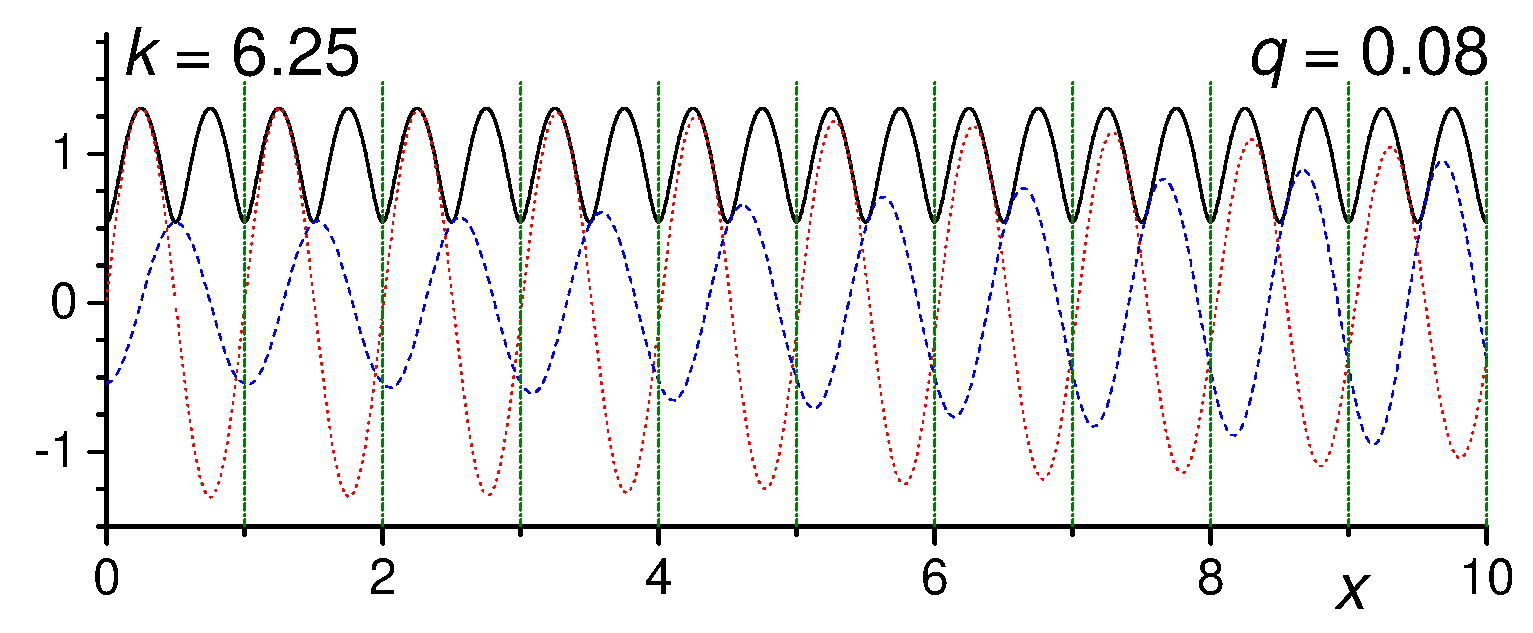
\epsfig{file=psi1e.eps,width=\linewidth}
            \end{subfigure}
            \hfill
            \begin{subfigure}{0.49\linewidth}
                \centering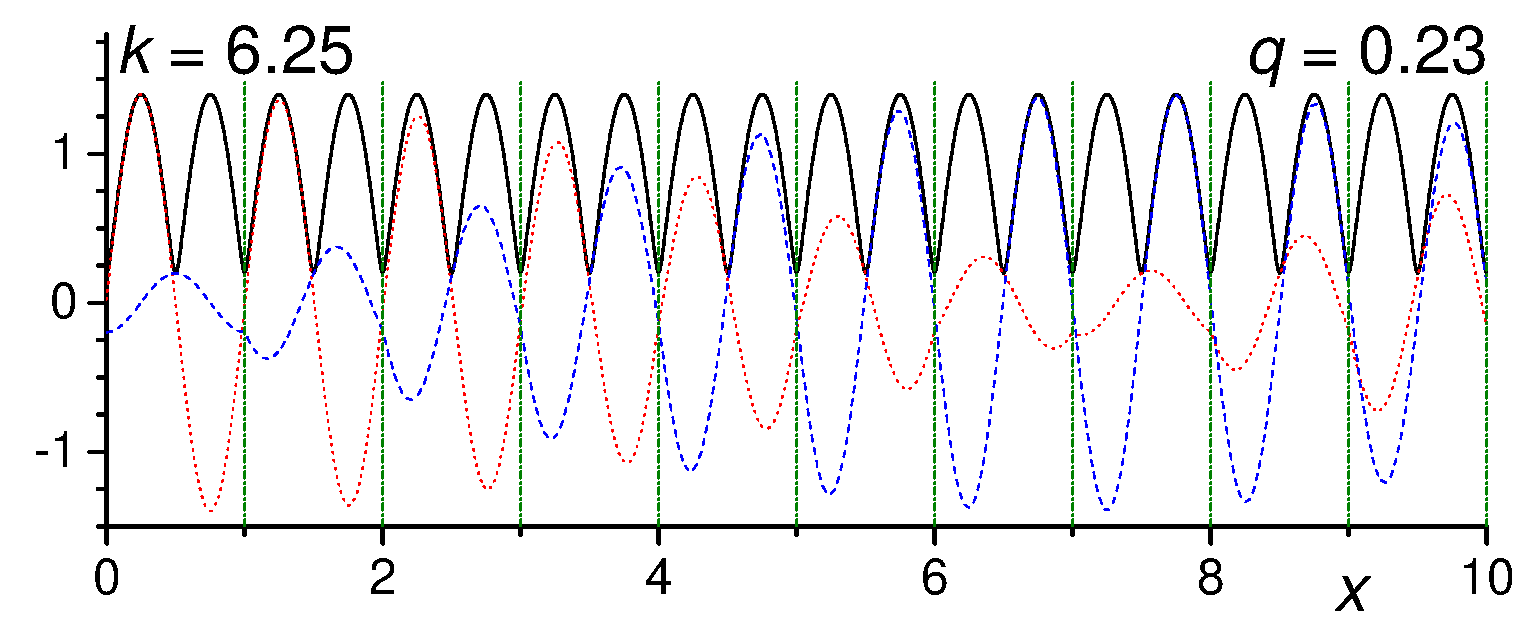
\epsfig{file=psi10e.eps,width=\linewidth}
            \end{subfigure}
            \scaption{
                Totéž jako v obrázku~\ref{fig:DiracCombWaveFunctions}, jen pro vlnové funkce z krajů 2. pásu.	
            }
            \label{fig:DiracCombWaveFunctions2Band}
        \end{figure}

        \begin{figure}[!htbp]
            \begin{subfigure}{0.49\linewidth}
                \centering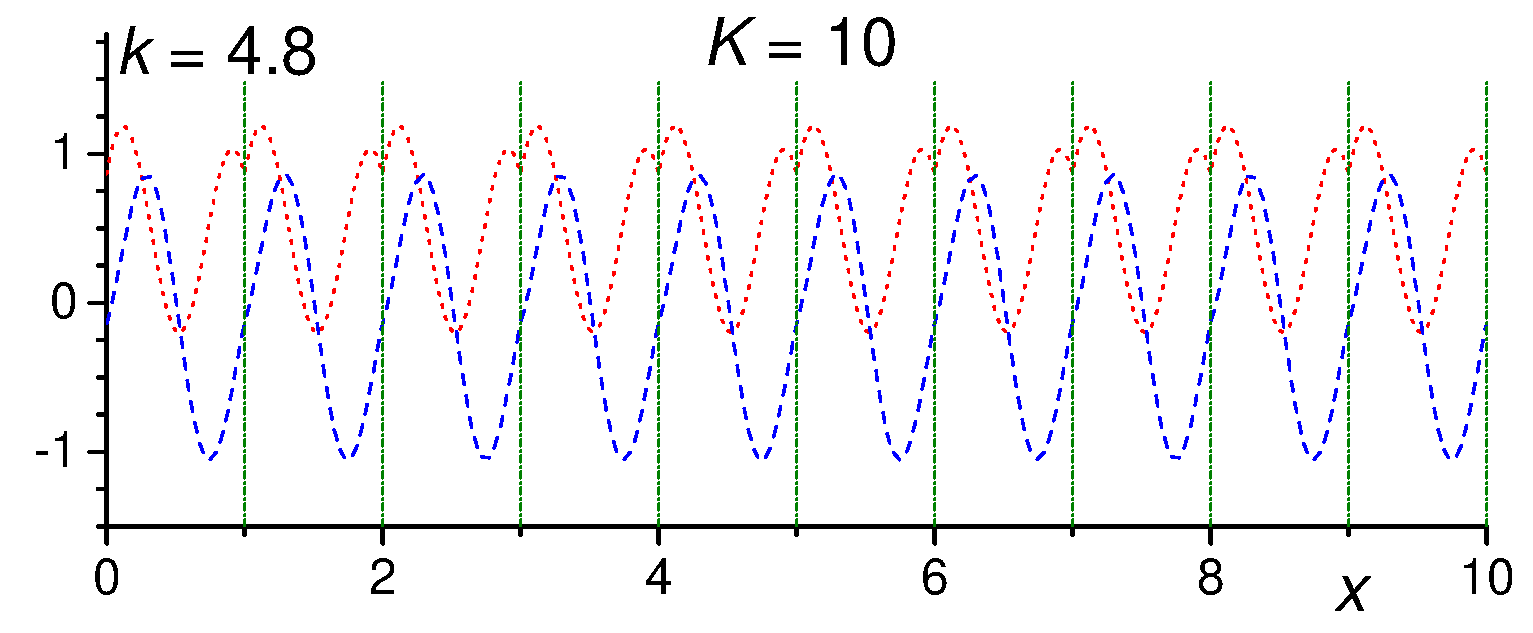
\epsfig{file=us.eps,width=\linewidth}
            \end{subfigure}
            \hfill
            \begin{subfigure}{0.49\linewidth}
                \centering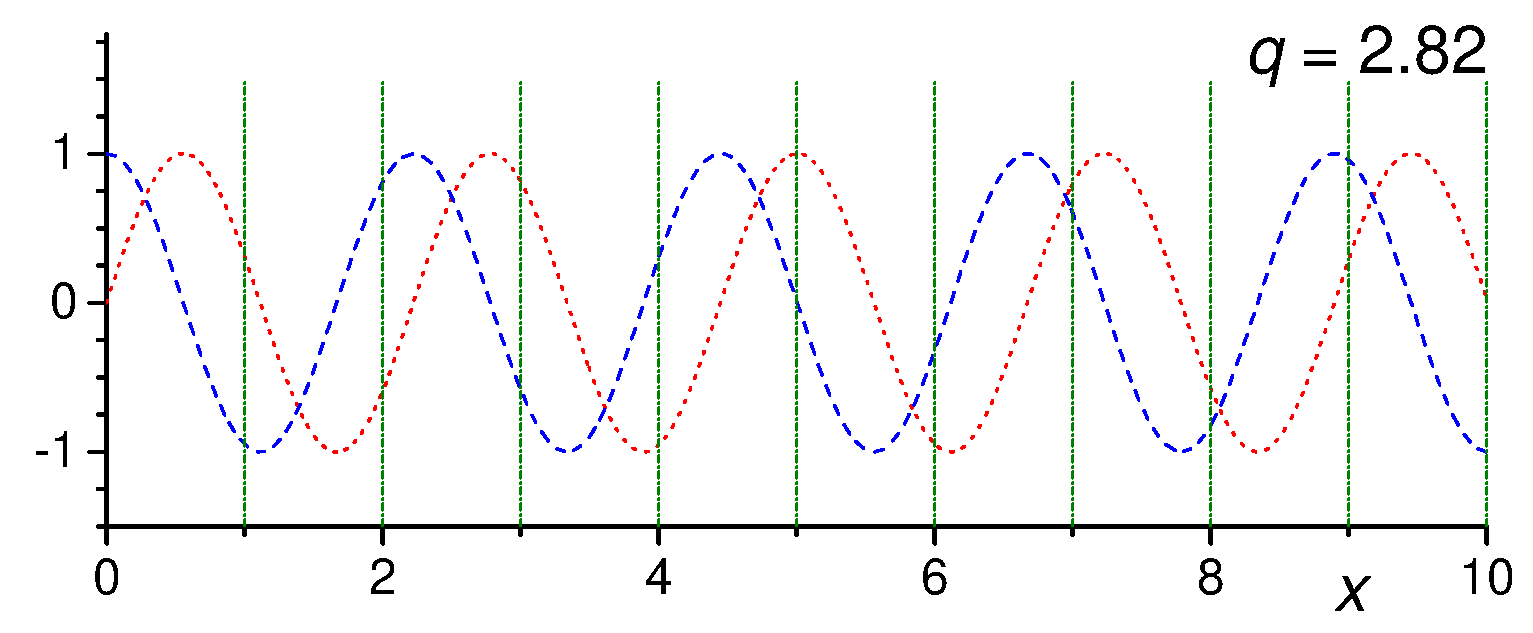
\epsfig{file=uqs.eps,width=\linewidth}
            \end{subfigure}
            \begin{subfigure}{0.49\linewidth}
                \centering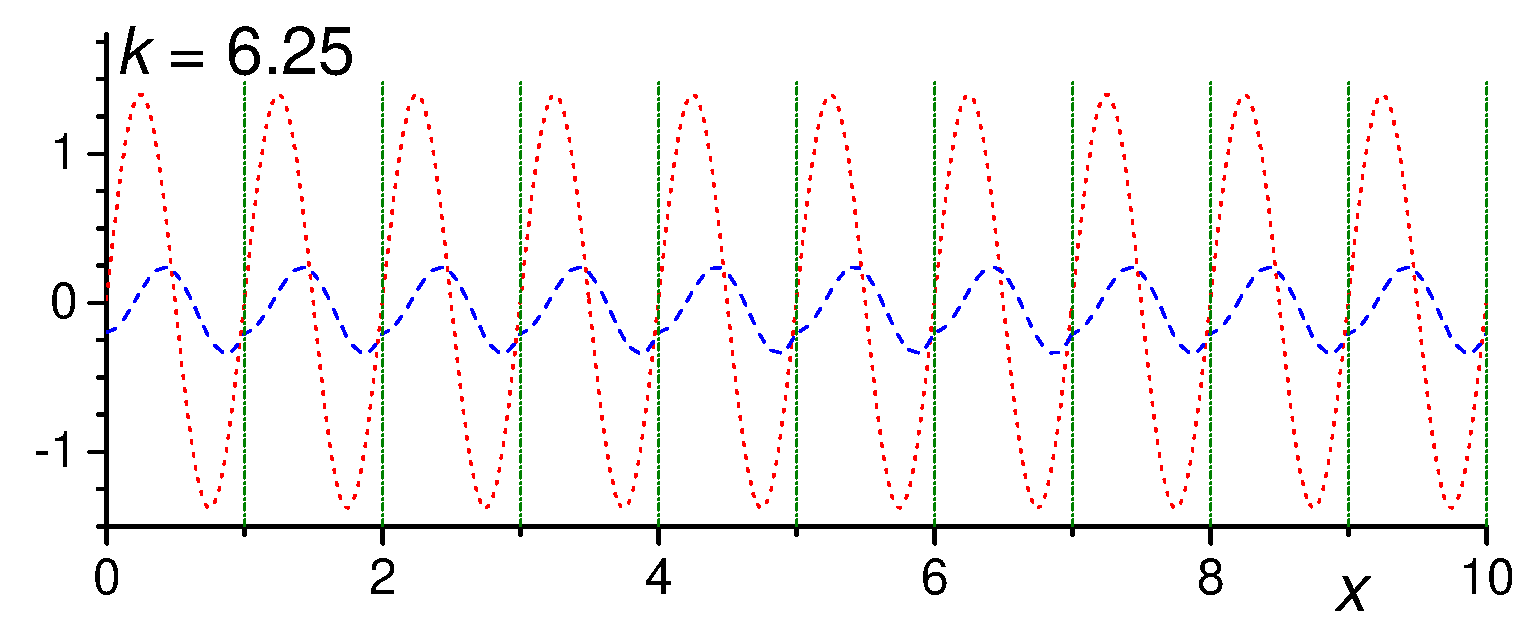
\epsfig{file=ue.eps,width=\linewidth}
            \end{subfigure}
            \hfill
            \begin{subfigure}{0.49\linewidth}
                \centering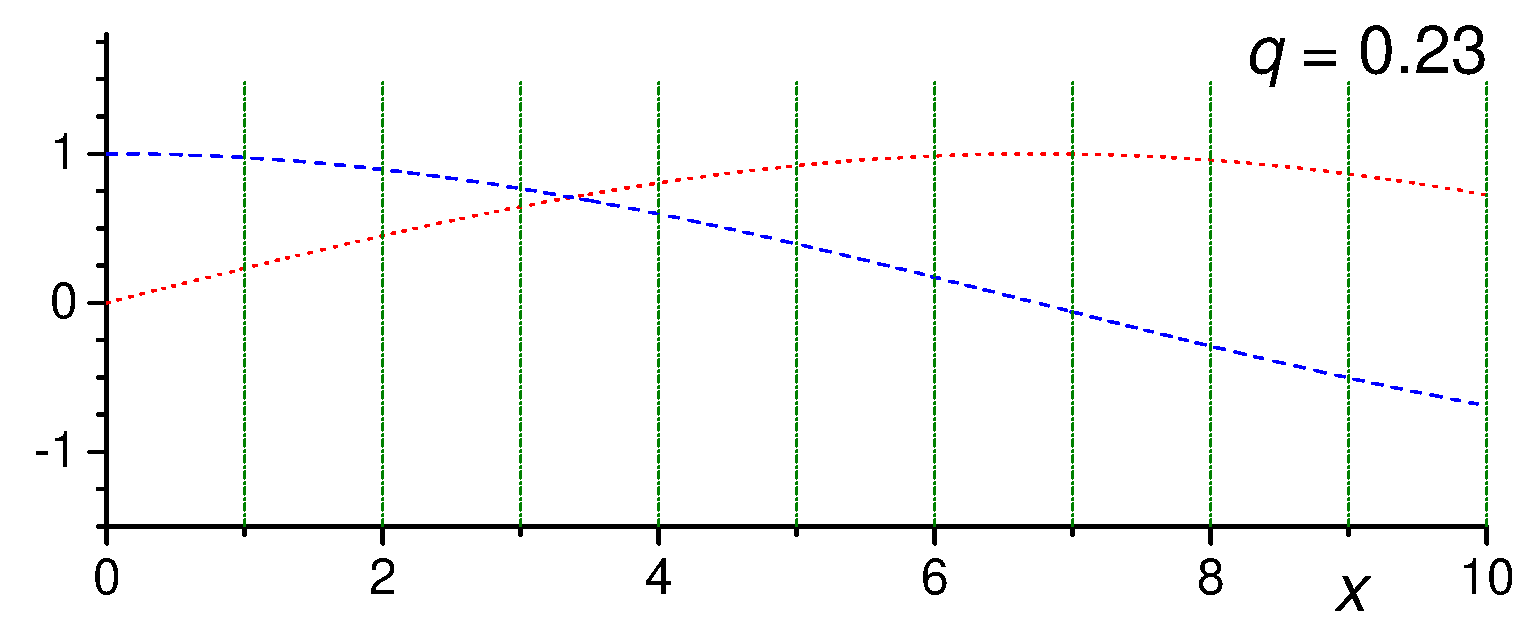
\epsfig{file=uqe.eps,width=\linewidth}
            \end{subfigure}
            \scaption{
                Periodická část vlnové funkce $u_{q}(x)$ (vlevo) a Blochova vlna $\e^{\im q x}$ (vpravo).
                Modrá čárkovaná čára -- reálná část, červená tečkovaná čára -- imaginární část.
                Pronásobení sloupců mezi sebou dá vlnové funkce z pravého sloupce obrázku~\ref{fig:DiracCombWaveFunctions2Band}.
            }
            \label{fig:DiracCombBlochWave}
        \end{figure}

        Podobně lze vyjádřit
        \begin{align}
            1&=2a\abs{A}^{2}\frac{1-\cos{qa}\cos{ka}+\frac{2}{Ka}\left(\cos{qa}-\cos{ka}\right)^{2}}{1-\cos{(q+k)a}},
        \end{align}
        takže normalizační konstanty jsou
        \begin{subequations}
            \begin{align}
                A&=s\sqrt{\frac{1}{2a}\frac{1-\cos{(q+k)a}}{1-\cos{qa}\cos{ka}+\frac{2}{Ka}\left(\cos{qa}-\cos{ka}\right)^{2}}}\e^{-\im\frac{ka}{2}},\\
                B&=\sqrt{\frac{1}{2a}\frac{1-\cos{(q-k)a}}{1-\cos{qa}\cos{ka}+\frac{2}{Ka}\left(\cos{qa}-\cos{ka}\right)^{2}}}\e^{\im\frac{ka}{2}},\\
                s&=\sign\left(\cos{qa}-\cos{ka}\right)
            \end{align}
        \end{subequations}
        (komplexní fáze se rozdělila stejným dílem mezi $A$ a $B$; je nutné udržet znaménko mezi $A$ a $B$).
        Získaný výsledek je v souladu s rovnicí (9) článku~\cite{Kronig1931}.
        
        Vlnová funkce normalizovaná na interval $(0,a)$ je tedy
        \begin{align}
            \psi_{q}(x)
                &=\frac{\e^{\im qna}}{\sqrt{2a}}\frac{1}{\sqrt{1-\cos{qa}\cos{ka}+\frac{2}{Ka}\left(\cos{qa}-\cos{ka}\right)^{2}}}\\
                &\qquad*\left[s\sqrt{1-\cos{(q+k)a}}\e^{\im k\left(x-na-\frac{a}{2}\right)}+\sqrt{1-\cos{(q-k)a}}\e^{-\im k\left(x-na-\frac{a}{2}\right)}\right].\nonumber
        \end{align}
        Několik příkladů vlnových funkcí je na obrázcích~\ref{fig:DiracCombWaveFunctions} a~\ref{fig:DiracCombWaveFunctions2Band}.
        Vlnová funkce rozložená na periodickou část a Blochovu vlnu je na obrázku~\ref{fig:DiracCombBlochWave}.
        Je vidět, že pro slabou interakci a střed pásu je pravděpodobnost nalezení částice prakticky konstantní (obrázek~\ref{fig:DiracCombWaveFunctions}, 1. sloupec, 3.--5. řádek).
        Naopak na krajích pásu nebo pro silnější interakci hustota pravděpodobnosti více osciluje (obrázek~\ref{fig:DiracCombWaveFunctions}, 2. sloupec, a obrázek~\ref{fig:DiracCombWaveFunctions2Band}).

    \item
        \begin{figure}[!htbp]
            \begin{subfigure}{0.49\linewidth}
                \centering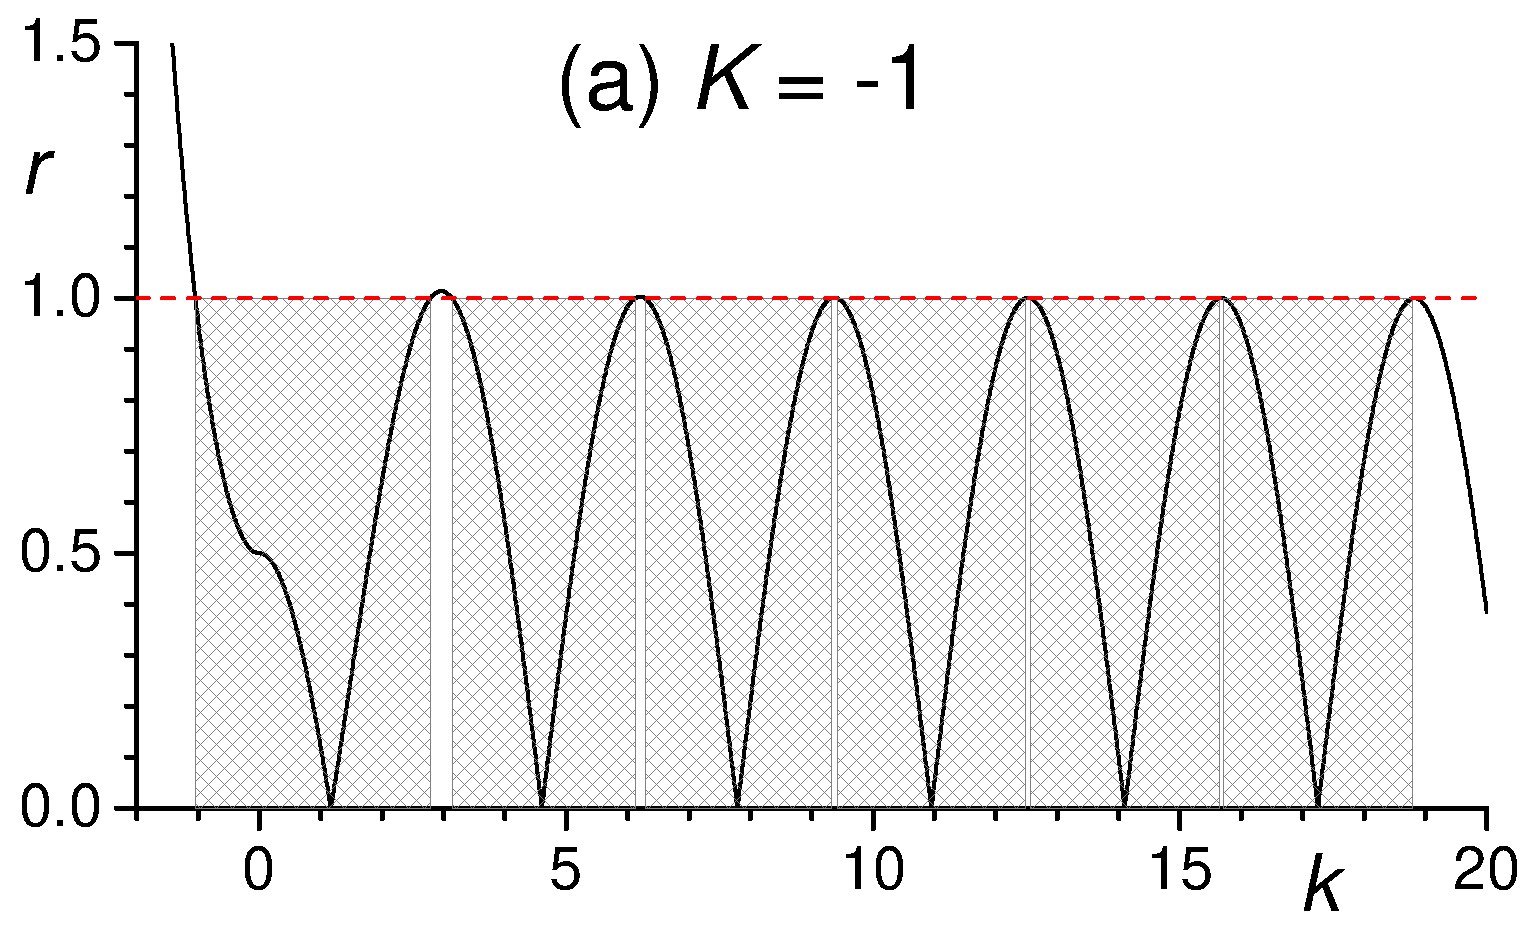
\epsfig{file=bandf1n.eps,width=\linewidth}
            \end{subfigure}
            \hfill
            \begin{subfigure}{0.49\linewidth}
                \centering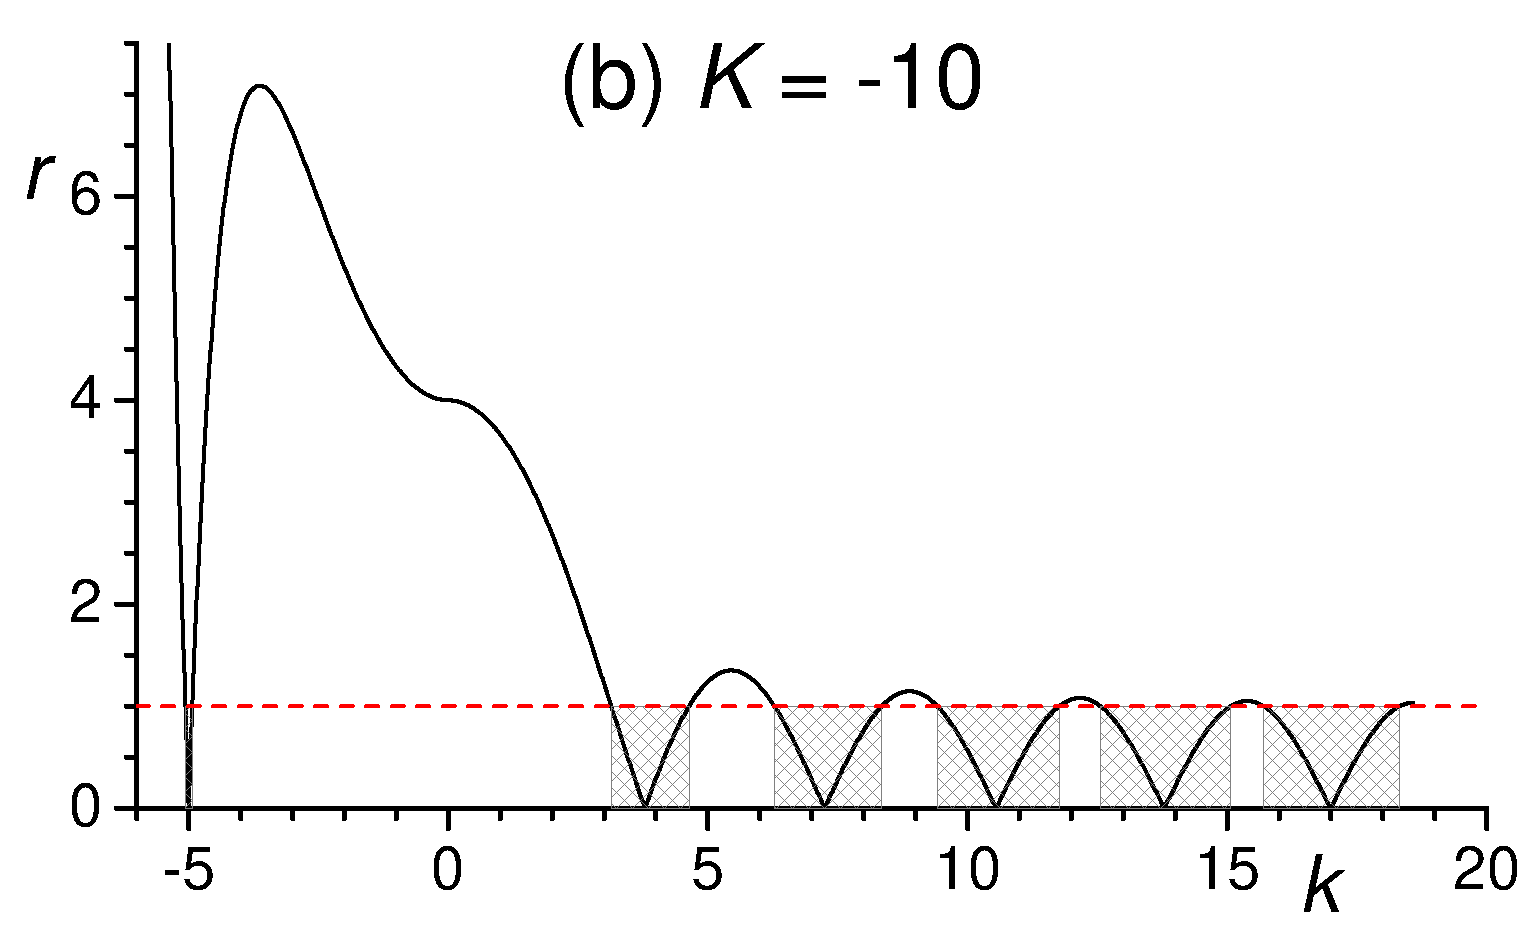
\epsfig{file=bandf10n.eps,width=\linewidth}
            \end{subfigure}
            \scaption{
                Funkce $r$ (černá čára) pro dvě záporné hodnoty parametru $K$ a mřížkovou konstantu $a=1$.
                Pásy, v nichž lze vyřešit rovnici~\eqref{eq:DiracCombBand} (pro $E<0$) a~\eqref{eq:DiracCombBandNegative} (pro $E>0$) jsou vyznačeny šrafováním.
            }
            \label{fig:DiracCombBandConditionNegative}
        \end{figure}

        \begin{figure}[!htbp]
            \begin{subfigure}{0.49\linewidth}
                \centering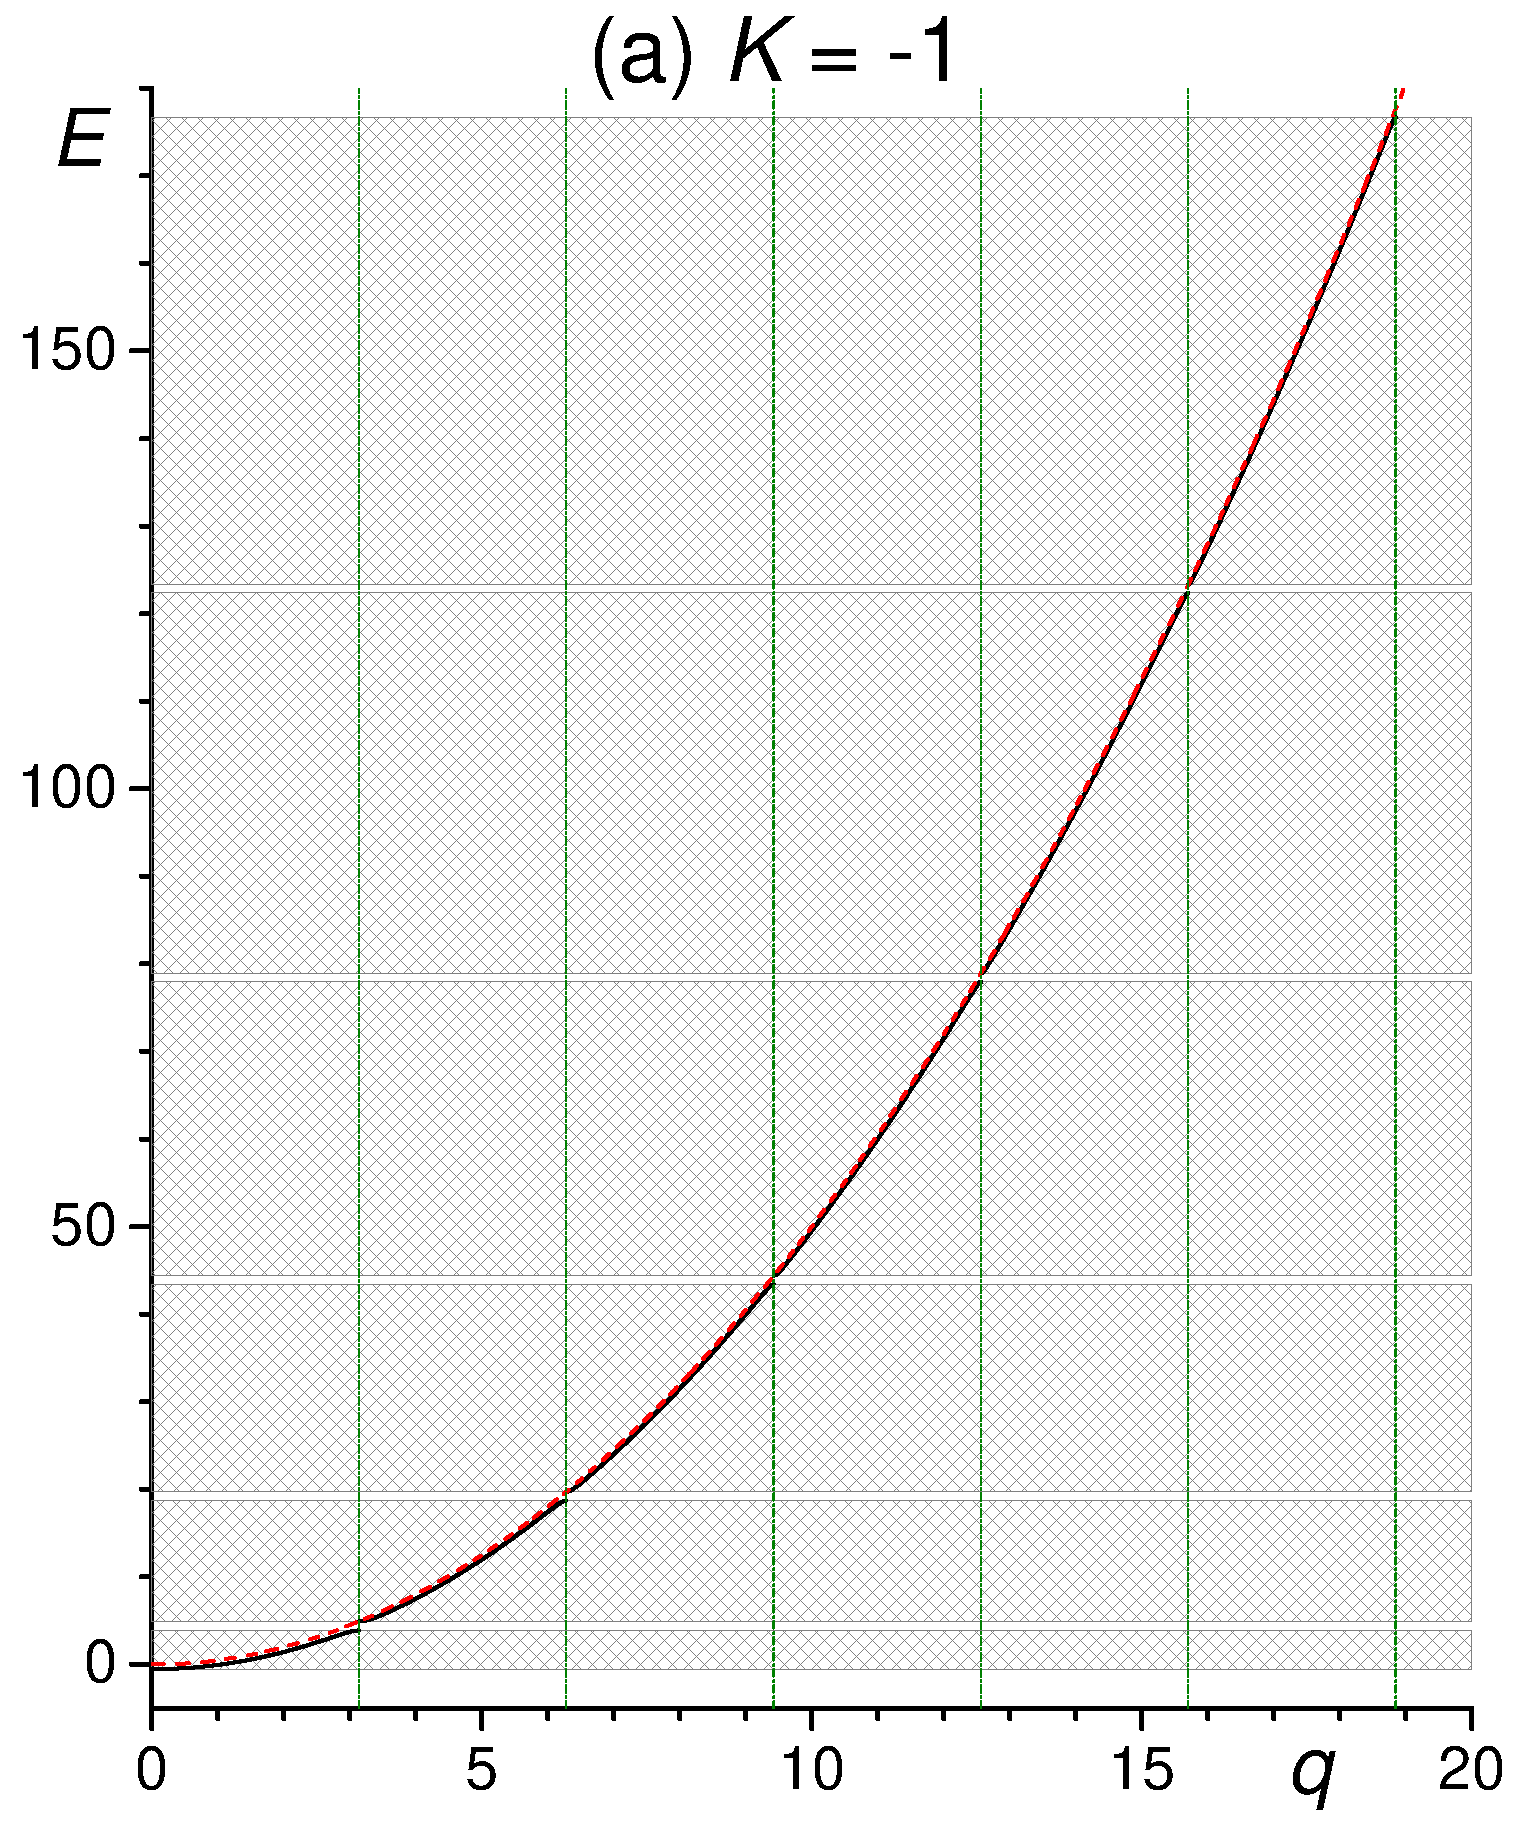
\epsfig{file=bands1n.eps,width=\linewidth}
            \end{subfigure}
            \hfill
            \begin{subfigure}{0.49\linewidth}
                \centering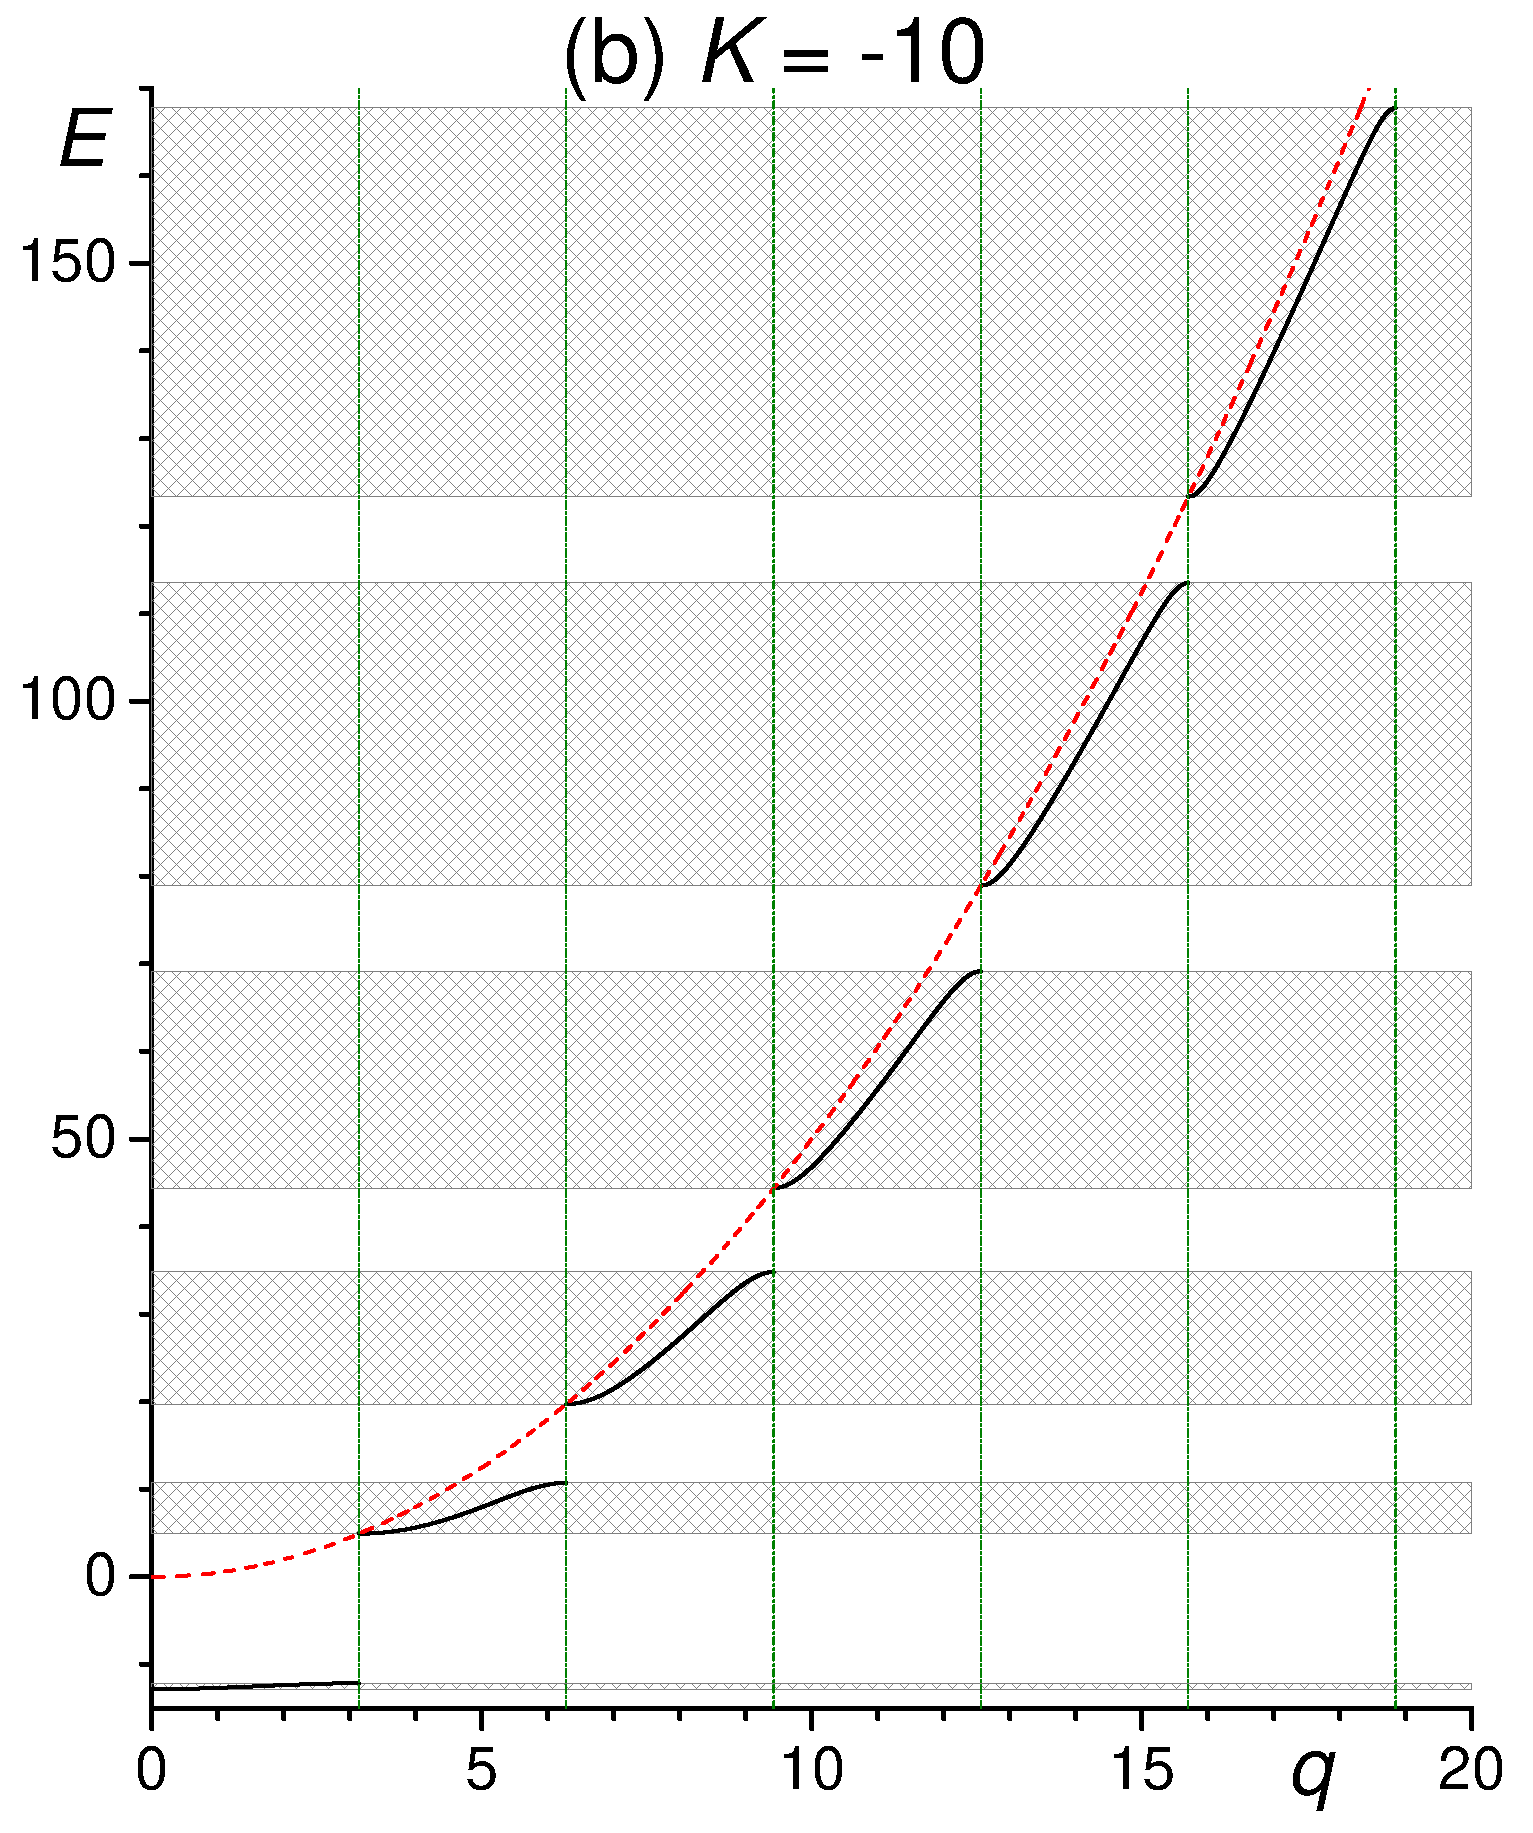
\epsfig{file=bands10n.eps,width=\linewidth}
            \end{subfigure}
            \begin{subfigure}{0.49\linewidth}
                \centering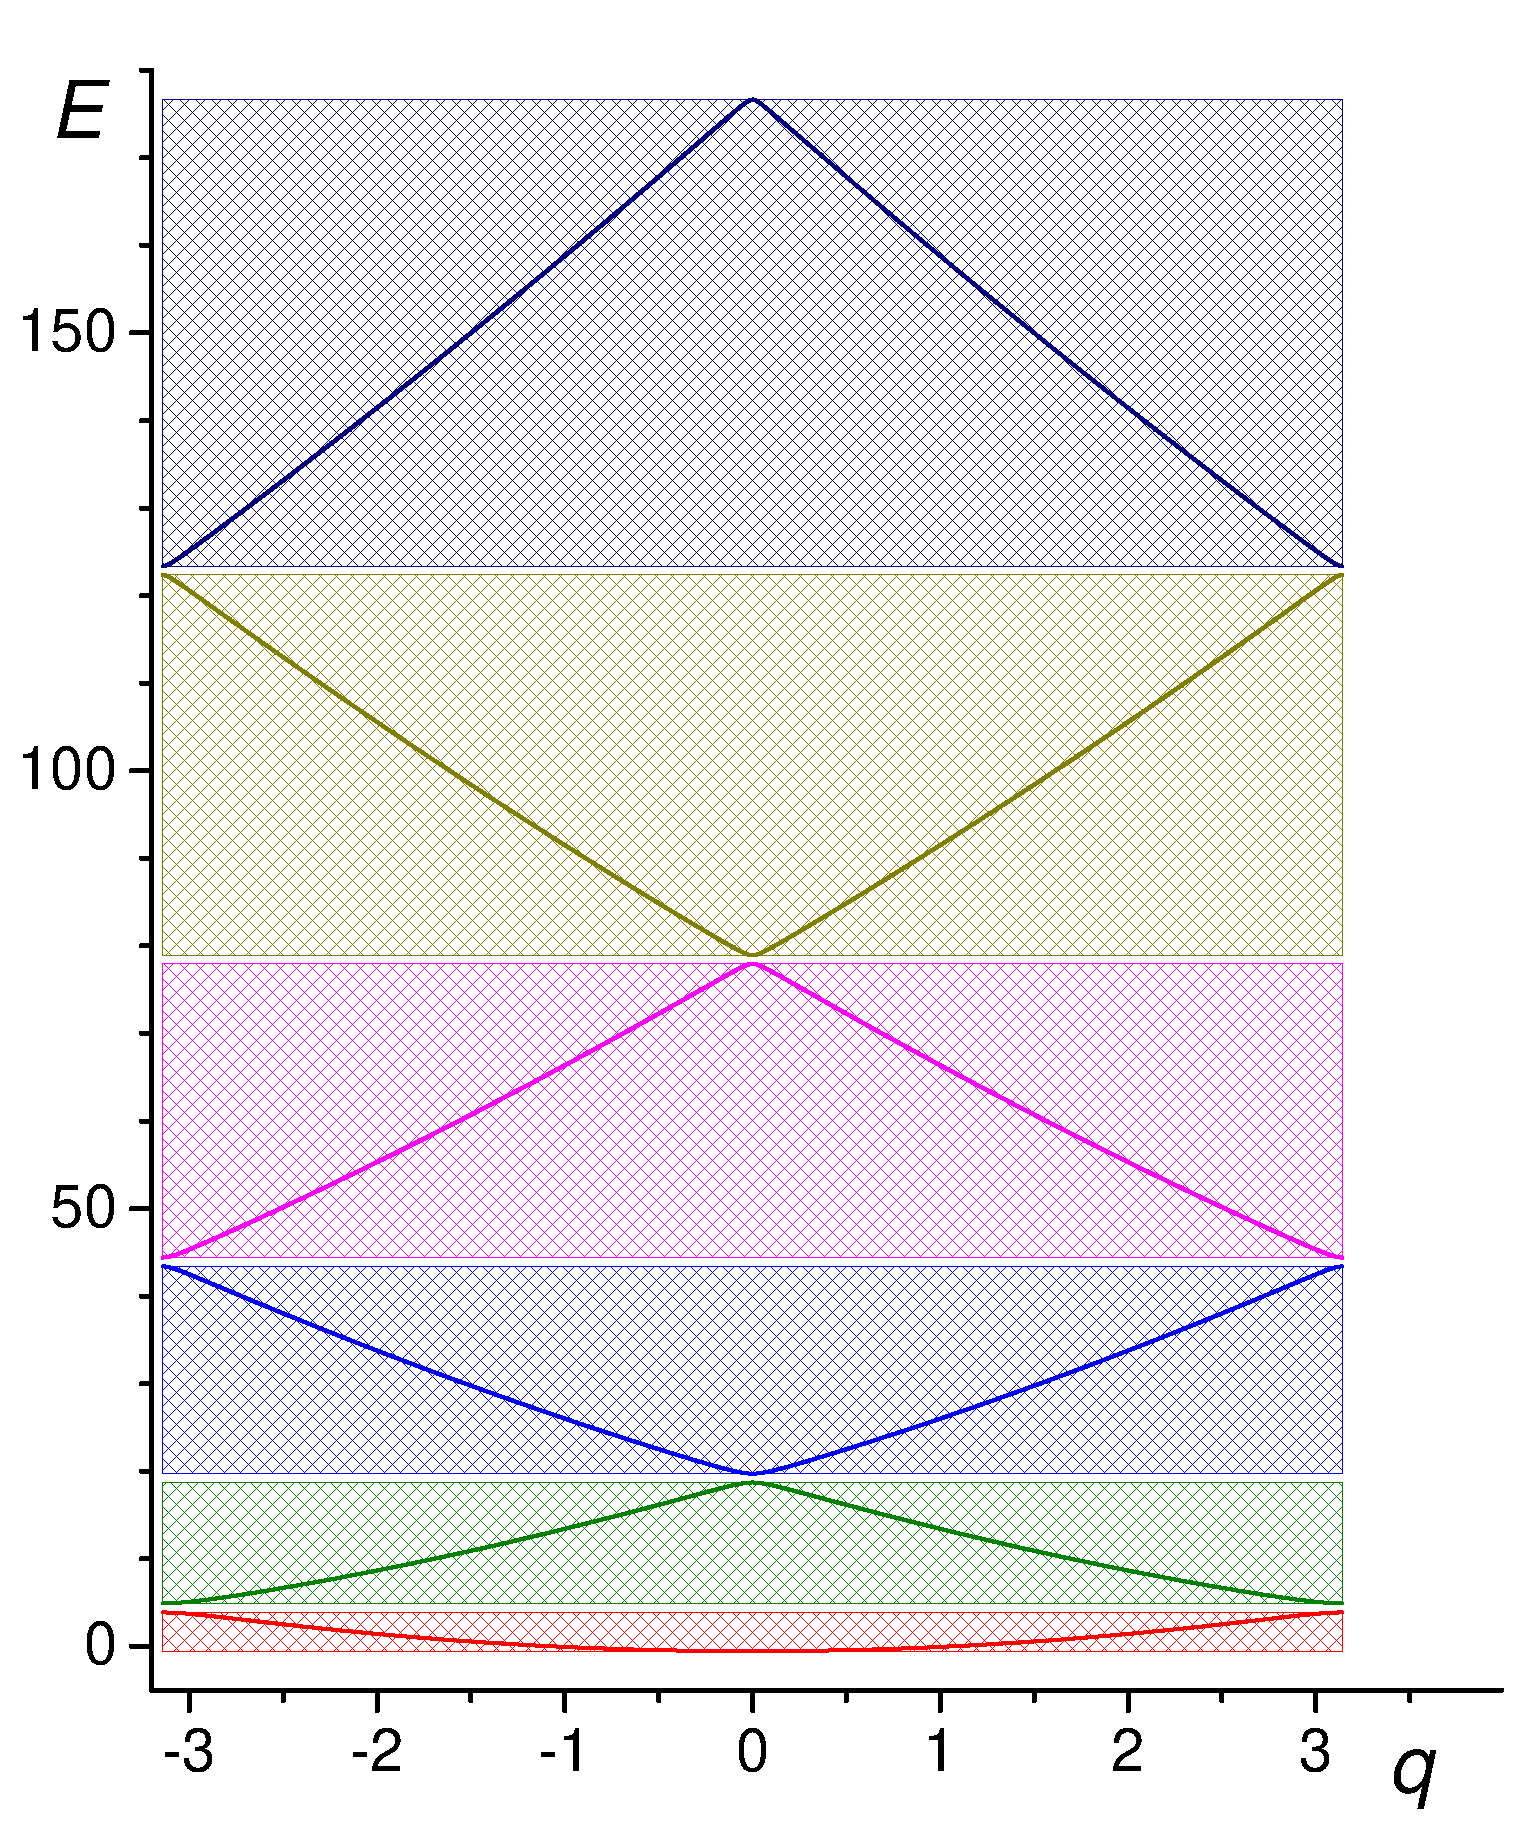
\epsfig{file=Brillouin1n.eps,width=\linewidth}
            \end{subfigure}
            \hfill
            \begin{subfigure}{0.49\linewidth}
                \centering\epsfig{file=Brillouin10n.eps,width=\linewidth}
            \end{subfigure}
            \scaption{
                \emph{1. řádek:} Disperzní relace v konvenci~\eqref{eq:DiracCombBandUnique} pro dvě hodnoty $K$ (černá čára).
                Červená čárkovaná čára odpovídá disperzní relaci pro volnou částici $E=\hbar^{2}q^{2}/(2M)$.
                Svislé zelené čerchované čáry vyznačují horní hranice pásů~\eqref{eq:DiracCombBandTop}.				
                Šrafováním jsou znázorněny povolené pásy.				
                \emph{2. řádek:}
                Disperzní relace pro 1. Brillouinovu zónu~\eqref{eq:Brillouin}.
                Jednotlivé pásy jsou znázorněny odlišnými barvami.
            }
            \label{fig:DiracCombBandsNegative}
        \end{figure}
        
        \begin{figure}[!htbp]
            \begin{subfigure}{0.49\linewidth}
                \centering\epsfig{file=vgE1n.eps,width=\linewidth}
            \end{subfigure}
            \hfill
            \begin{subfigure}{0.49\linewidth}
                \centering\epsfig{file=vgE10n.eps,width=\linewidth}
            \end{subfigure}
            \begin{subfigure}{0.49\linewidth}
                \centering\epsfig{file=vgq1n.eps,width=\linewidth}
            \end{subfigure}
            \hfill
            \begin{subfigure}{0.49\linewidth}
                \centering\epsfig{file=vgq10n.eps,width=\linewidth}
            \end{subfigure}
            \scaption{
                Grupová rychlost~\eqref{eq:DiracCombGroupVelocity} v závislosti na energii (1. řádek) a na kvazihybnosti (2. řádek).
                Ve 2. řádku jsou hranice pásů $q=\pi n$ znázorněny svislými zelenými čerchovanými čarami.
                Červená čárkovaná čára odpovídá rychosti pro volnou částici $E=\hbar q/M$.
            }
            \label{fig:DiracCombGroupVelocityNegative}
        \end{figure}

        V souladu s případem izolovaných $\delta$ jam (viz příklady~\ref{sec:Delta} a~\ref{sec:DoubleDelta}) se označí
        \begin{equation}
            \kappa=\sqrt{-\frac{2ME}{\hbar^{2}}}.
        \end{equation}
        Formálně tedy platí $k=\im\kappa$, čehož lze využít v rovnici~\eqref{eq:DiracCombBand} a dojít k podmínce
        \begin{equation}\label{eq:DiracCombBandNegative}
            \boxed{\cos{qa}=\cosh{\kappa a}+\frac{K}{2\kappa}\sinh{\kappa a}}.
        \end{equation}
        Pro $K\in(-\frac{4}{a},0)$ leží nulová energie v nejnižším pásu.
        Pokud $K<-\frac{4}{a}$, první povolený pás se nachází na enegii $E<0$ a na energii $E=0$ je zakázaný pás.
        
        V analogii s obrázky~\ref{fig:DiracCombBands}---\ref{fig:DiracCombGroupVelocity} je na obrázcích~\ref{fig:DiracCombBandsNegative}---\ref{fig:DiracCombGroupVelocityNegative} zobrazen průběh veličiny $r$, disperzní relace $E(q)$ v konvenci~\eqref{eq:DiracCombBandUnique} a v 1. Brillouinově zóně a grupová rychlost pro dvě záporné hodnoty síly interakce $K$.

    \end{enumerate}
\end{solution}
    

\np
%\section{Potenciály s $\delta$-funkcemi II}
\exercise[24.11.2021, 25.11.2021]{Diracův hřeben}
 	Částice se pohybuje v potenciálu složeném z periodicky se opakujících $\delta$ funkcí
 	\begin{equation*}
 		V(x)=c\sum_{n=-\infty}^{\infty}\delta(x-na),
 	\end{equation*}
 	jehož vlnové funkce na intervalu 
 	$x\in\left(na; \left(n+1\right)a\right)$, $n\in\mathbb{Z}$, $c>0$, $E>0$ 
 	jsou podle Blochova teorému
 	\begin{equation*}
 		\psi_{q}(x)
 			=\left[A\e^{\im k\left(x-na\right)}+B\e^{-\im k\left(x-na\right)}\right]\e^{iqna},
 	\end{equation*}
 	kde $q$ je krystalová hybnost (kvazihybnost) částice.
 	Mezi $k=\sqrt{2ME}/\hbar$ a $K$ platí vztah
 	\begin{equation*}
 		\cos{qa}=\cos{ka}+\frac{K}{2k}\sin{ka},
 	\end{equation*}
 	kde $K=2Mc/\hbar^{2}$ ($M$ je hmotnost částice).
 	\begin{enumerate}
 	\item 
 		Pro dvě hodnoty $K=2$ a $K=10$ vypočítejte a zakreslete do grafu disperzní relaci $E(q)$ pro nejnižší čtyři energetické pásy.
 		Uvažujte následující konvenci: pokud $\pi n\leq ka\leq\pi(n+1)$, pak $\pi n\leq qa\leq\pi(n+1)$, $n\in\mathbb{Z}$.
 	\item 
 		Vypočítejte grupovou rychlost
 		\begin{equation*}
 			v_{\ti{g}}=\frac{1}{\hbar}\frac{\partial E}{\partial q}
 		\end{equation*}
 		a zakreslete její závislost na $q$ a na $E$ pro dvě hodnoty parametru $K=2$, $K=10$ a nejnižší čtyři energetické pásy.
 		Srovnejte s případem volné částice.
 	\item
 		Najděte řešení Schrödingerovy rovnice pro případ $K<0$ (v tomto případě může být energie i záporná).
 		Podobně jako v bodě 1 zakreslete disperzní relaci $E(q)$ pro $K=-2$ a $K=-10$.

 	\item 
 		Nalezněte parametry $A$, $B$ vlnové funkce. Vlnovou funkci normalizujte na intervalu mezi sousedními dvěma $\delta$ funkcemi:
 		\begin{equation*}
 			\label{eq:psiqnorm}
 			\int_{0}^{a}\abs{\psi_{q}(x)}^{2}\d x=1.
 		\end{equation*}
 	\end{enumerate}

 	Pro všechny numerické výpočty uvažujte $a=M=\hbar=1$.\np

\section{Koherentní stavy harmonického oscilátoru}
\sectionmark{Koherentní stavy}
\label{sec:CoherentStates}

\begin{theory}
V této části se navazuje zejména na kapitolu~\ref{sec:HO} o algebraickém řešení harmonického oscilátoru.
Cílem je prozkoumat vlastnosti \emph{koherentního stavu}\index{stav!koherentní} jednorozměrného harmonického oscilátoru
\begin{equation}
	\label{eq:HOCoherentState}
	\important{\ket{z}=\e^{-\frac{|z|^{2}}{2}}\sum_{n=0}^{\infty}\frac{z^{n}}{\sqrt{n!}}\ket{n}}\,,
\end{equation}
kde $z\in\mathbb{C}$ je libovolné komplexní číslo a $\ket{n}$ je vlastní stav harmonického oscilátoru~\eqref{eq:NumberOperator} příslušející energii $E_{n}$, dané vztahem~\eqref{eq:HOEnergy}.

Níže uvedený postup je deduktivní a vychází z definice koherentního stavu~\eqref{eq:HOCoherentState}.
Dá se však postupovat i opačně: (i) buď hledat stavy harmonického oscilátoru, které minimalizují relace neurčitosti~\eqref{eq:HOCoherentStateUncertainty}, jak je popsáno v práci~\cite{Formanek2004} (strana 220), nebo hledat takové stavy, které co nejlépe aproximují pohyb klasické částice, tj. splňují vztah~\eqref{eq:HOCoherentStateClassicalMotion} pro střední hodnoty $\operator{x}$ a $\operator{p}$.
Tento postup je sledován například v učebnici~\cite{Manoukian2006}.
\end{theory}

\subsection{Poissonovo rozdělení}
\label{sec:PoissonDistribution}
Poissonovo rozdělení\index{rozdělení!Poissonovo} udává počet $n$ výskytu jevů v určitém intervalu, pokud jsou jednotlivé jevy statisticky nezávislé.
Rozdělení je dáno předpisem
\begin{equation}
    \label{eq:PoissonDistribution}
    P_{n}=\frac{\lambda^{n}}{n!}\e^{-\lambda}\,,
\end{equation}			
kde $\lambda$ je parametr Poissonova rozdělení.

\begin{enumerate}
\item
    Ukažte, že rozdělení je normalizované.
    
\item
    Nalezněte střední hodnotu Poissonova rozdělení.
    
\item
    Nalezněte rozptyl Poissonova rozdělení.
\end{enumerate}

\begin{solution}
    \begin{enumerate}
	\item
		Normalizace
		\begin{equation}
			\sum_{n=0}^{\infty}P_{n}
				=\sum_{n=0}^{\infty}\frac{\lambda^{n}}{n!}
				=\e^{-\lambda}\e^{\lambda}=1\,.
		\end{equation}
		
	\item
		Střední hodnota
		\begin{equation}
			\mean{n}
				=\sum_{n=0}^{\infty}nP_{n}
				=\e^{-\lambda}\sum_{n=1}^{\infty}\frac{\lambda^{n}}{(n-1)!}
				=\e^{-\lambda}\lambda\e^{\lambda}=\lambda\,.
		\end{equation}
		
	\item
		Střední hodnota kvadrátu je
		\begin{align}
			\mean{n^{2}}
				&=\sum_{n=0}^{\infty}n^{2}P_{n}
				=\e^{-\lambda}\sum_{n=1}^{\infty}\frac{\lambda^{n}}{(n-1)!}
					\underbrace{n}_{n-1+1}\nonumber\\
				&=\e^{-\lambda}\left[\lambda^{2}\sum_{n=2}^{\infty}\frac{\lambda^{n-2}}{(n-2)!}
					+\lambda\sum_{n=1}^{\infty}\frac{\lambda^{n-1}}{(n-1)!}\right]\nonumber\\
				&=\lambda^{2}+\lambda\,,
		\end{align}
		takže rozptyl vychází
		\begin{equation}
			(\Delta n)^{2}=\mean{n^{2}}-\mean{n}^{2}=\lambda\,.
		\end{equation}
		Poissonovo rozdělení má tedy rozpyl i střední hodnotu stejnou a danou velikostí parametru $\lambda$.
	\end{enumerate}
\end{solution}

\subsection{Základní vlastnosti koherentních stavů}
\label{sec:HOCoherentState}
\begin{enumerate}
\item 
    Ukažte, že skalární součin dvou koherentních stavů~\eqref{eq:HOCoherentState} je
    \begin{equation}			
        \label{eq:HOCoherentStateBraket}
        \braket{z}{z'}=\e^{-\frac{\abs{z-z'}^{2}}{2}
            +\im\abs{z}\abs{z'}\sin\left(\phi'-\phi\right)}\,,
    \end{equation}
    kde
    \begin{equation}
        \label{eq:z}
        z=\abs{z}\e^{\im\phi}\,,\qquad\phi\in[0,2\pi)\,.
    \end{equation}
    Koherentní stavy jsou tedy normalizované, avšak nejsou navzájem ortogonální, z čehož vyplývá, že $\ket{z}$ nelze vzít za bázi Hilbertova prostoru harmonického oscilátoru (resp. někdy se říká, že báze pomocí koherentních stavů je přeurčená).

\item
    Ukažte, čemu se rovná pravděpodobnost nalezení stavu $\ket{z'}$, 
    pokud máme systém připravený ve stavu $\ket{z}$.

\item
    Ukažte, že je splněna relace uzavřenosti ve tvaru
    \begin{equation}
        \int\ket{z}\bra{z}\frac{\d z}{\pi}=1\,.
    \end{equation}

\item
    Ukažte, že rozdělení energií v koherentním stavu je Poissonovo, tj. že lze psát
    \begin{equation}
        P_{n}=\abs{\braket{n}{z}}^{2}=\frac{\lambda^{n}}{n!}\e^{-\lambda}\,.
    \end{equation}
    Nalezněte $\lambda$.

\item 
    Na základě vlastností Poissonova rozdělení nalezněte, 
    čemu se rovná střední hodnota energie harmonického oscilátoru
    v koherentním stavu $\mean{E}_{z}$.
\end{enumerate}
	
\begin{solution}
	\begin{enumerate}
	\item
		Na základě definice~\eqref{eq:HOCoherentState} platí:
		\begin{align}
			\braket{z}{z'}
				&=\e^{-\frac{\abs{z}^{2}+\abs{z'}^{2}}{2}}
					\sum_{n,n'=0}^{\infty}\frac{(z^{*})^{n}(z')^{n'}}{\sqrt{n!n'!}}
					\underbrace{\braket{n}{n'}}_{\delta_{nn'}}\nonumber\\
				&=\e^{-\frac{\abs{z}^{2}+\abs{z'}^{2}}{2}}
					\sum_{n=0}^{\infty}\frac{(z^{*}z')^{n}}{n!}\,.
		\end{align}
		Po zavedení
		\begin{equation}
			z^{*}=\abs{z}\e^{-\im\phi}\,,\qquad z'=\abs{z'}\e^{\im\phi'}			
		\end{equation}
		lze absolutní hodnotu rozdílu dvou komplexních čísel rozepsat jako
		\begin{align}
			\abs{z-z'}^{2}
				&=\left(z-z'\right)\left(z^{*}-z'^{*}\right)\nonumber\\
				&=\abs{z}^{2}+\abs{z'}^{2}-zz'^{*}-z^{*}z'\nonumber\\
				&=\abs{z}^{2}+\abs{z'}^{2}-\abs{z}\abs{z'}\e^{\im(\phi-\phi')}
					-\abs{z}\abs{z'}\e^{-\im(\phi-\phi')}\nonumber\\
				&=\abs{z}^{2}+\abs{z'}^{2}-2\abs{z}\abs{z'}\cos{(\phi-\phi')}\,.
		\end{align}		
		Pak
		\begin{align}
			\braket{z}{z'}
				&=\e^{-\frac{\abs{z}^{2}+\abs{z'}^{2}}{2}}\sum_{n=0}^{\infty}
					\frac{\abs{z}^{n}\abs{z'}^{n}}{n!}\e^{\im n(\phi'-\phi)}\nonumber\\
				&=\e^{-\frac{\abs{z}^{2}+\abs{z'}^{2}}{2}}\sum_{n=0}^{\infty}
					\frac{\left[\abs{z}\abs{z'}\e^{\im(\phi'-\phi)}\right]^{n}}{n!}\nonumber\\
				&=\e^{-\frac{\abs{z}^{2}+\abs{z'}^{2}}{2}}\e^{\abs{z}\abs{z'}
					\left[\cos{(\phi'-\phi)}+\im\sin{(\phi'-\phi)}\right]}\nonumber\\
				&=\e^{-\frac{\abs{z'-z}^{2}}{2}+\im\abs{z}\abs{z'}\sin{(\phi'-\phi)}}\,.
		\end{align}
		Je tedy $\braket{z}{z}=1$, avšak $\braket{z}{z'}\neq 0$ je obecně nenulové komplexní číslo.
		
	\item
		Hledaná pravděpodobnost je dána kvadrátem amplitudy~\eqref{eq:HOCoherentStateBraket}
		\begin{equation}
			p=\abss{\braket{z'}{z}}=\e^{-\abs{z'-z}}\,.
		\end{equation}
	
	\item
		Komplexní číslo $z$ se opět vyjádří pomocí velikosti a fáze~\eqref{eq:z}, 
		kde pro zjednodušení zápisu označíme $r\equiv\abs{z}$.
		Pak $\d z=r\d r\d\phi$ a integrál relací uzavřenosti dá
		\begin{align}
			\int\ket{z}\bra{z}\frac{\d z}{\pi}
				&=\int\e^{-r^{2}}\sum_{n,n'=0}^{\infty}\frac{r^{n}\e^{\im n\phi}}{\sqrt{n!}}
					\frac{r^{n'}\e^{-\im n'\phi}}{\sqrt{n'!}}\ket{n}\bra{n'}
					\frac{r}{\pi}\,\d r\d\phi\nonumber\\
				&=\sum_{n,n'=0}^{\infty}\frac{\ket{n}\bra{n'}}{\pi\sqrt{n!n'!}}
					\underbrace{\int_{0}^{\infty}\e^{-r^{2}}r^{n+n'+1}\d r}_{\rho\equiv r^{2}\,,
					\quad\d\rho=2r\d r}
					\underbrace{\int_{0}^{2\pi}\e^{\im(n-n')\phi}\d\phi}_{2\pi\delta_{nn'}}\nonumber\\
				&=\sum_{n=0}^{\infty}\frac{2\ket{n}\bra{n}}{n!}\frac{1}{2}
					\underbrace{\int_{0}^{\infty}\rho^{n}\e^{-n}\d\rho}_{\Gamma(n+1)=n!}\nonumber\\
				&=\sum_{n=0}^{\infty}\ket{n}\bra{n}=1\,.
		\end{align}
		
	\item
		Pravděpodobnost se získá dosazením do definičního vztahu~\eqref{eq:HOCoherentStateBraket}
		\begin{equation}
			P_{n}
				=\abs{\braket{n}{z}}^{2}
				=\abs{\e^{-\frac{\abs{z}^{2}}{2}}\frac{z^{n}}{\sqrt{n!}}}^{2}\nonumber\\
				=\e^{-\abs{z}^{2}}\frac{\abs{z}^{2n}}{n!}
		\end{equation}
		a srovnáním s Poissonovým rozdělením~\eqref{eq:PoissonDistribution}
		\begin{equation}
			\lambda=\abs{z}^{2}\,.
		\end{equation}			
		
	\item
		Energie vlastního stavu harmonického oscilátor $\ket{n}$ je dána vztahem~\eqref{eq:HOEnergy}.
		Po dosazení
		\begin{equation}
			\label{eq:HOmeanE}
			\mean{E}_{z}				
				=\sum_{n=0}^{\infty}\hbar\Omega\left(n+\frac{1}{2}\right)\e^{-\lambda}
					\frac{\lambda^{n}}{n!}
				=\hbar\Omega\left(\lambda+\frac{1}{2}\right)
				=\hbar\Omega\left(\abs{z}^{2}+\frac{1}{2}\right)\,.
		\end{equation}	
	\end{enumerate}
\end{solution}

\subsection{Vlastní stav operátoru $\operator{a}$}
\begin{enumerate}
\item 
    Ukažte, že pro posunovací operátor $\operator{a}$ platí
    \begin{equation}
        \label{eq:HOCoherentStateA}
        \important{\operator{a}\ket{z}=z\ket{z}}\,.
    \end{equation}
    To znamená, že koherentní stav $\ket{z}$ je vlastním stavem $\operator{a}$ 
    s vlastní hodnotou $z$.
    Operátor $\operator{a}$ není hermitovský, proto jsou jeho vlastní hodnoty komplexní.

\item 
    Ukažte, že neexistuje žádný vlastní stav posunovacího operátoru $\conjugate{\operator{a}}$.

\item 
    Pomocí Bakerovy-Campbellovy-Hausdorffovy formule~\eqref{eq:BCH1} ukažte, 
    že koherentní stav lze vyjádřit také ve tvaru
    \begin{equation}
        \ket{z}=\e^{z\conjugate{\operator{a}}-z^{*}\operator{a}}\ket{0}.
    \end{equation}
\end{enumerate}

\begin{solution}
    \begin{enumerate}
		\item 
			Při důkazu se vychází z definice koherentního stavu~\eqref{eq:HOCoherentState} a vztahu pro posunovací operátor~\eqref{eq:AN}:
			\begin{align}
				\operator{a}\ket{z}
					&=\e^{-\frac{\abs{z}^{2}}{2}}\sum_{n=0}^{\infty}
						\frac{z^{n}}{\sqrt{n!}}\underbrace{\operator{a}\ket{n}}_{\sqrt{n}\ket{n-1}}\nonumber\\
					&=z\e^{-\frac{\abs{z}^{2}}{2}}\sum_{n=1}^{\infty}
						\frac{z^{n-1}}{\sqrt{(n-1)!}}\ket{n-1}\nonumber\\
					&=z\ket{z}\,.
			\end{align}
		
		\item
			Předpokládejme, že existuje vlastní stav operátoru $\conjugate{\operator{a}}$ s vlastní hodnotou $\lambda$
			\begin{equation}
				\conjugate{\operator{a}}\ket{\psi(z)}=z\ket{\psi(z)}\,,
			\end{equation}
			který lze vyjádřit v bázi $\ket{n}$ jako rozvoj
			\begin{equation}
				\label{eq:cohac}
				\ket{\psi(z)}=\sum_{n=0}^{\infty}a_{n}\frac{z^{n}}{\sqrt{n!}}\ket{n}\,.
			\end{equation}
			Působení $\conjugate{\operator{a}}$ na tento vztah dá
			\begin{equation}
				\conjugate{\operator{a}}\ket{\psi(z)}=\sum_{n=0}^{\infty}a_{n}\frac{z^{n}}{(n+1)!}\ket{n+1}\,,
			\end{equation}
			takže v rozvoji~\eqref{eq:cohac} musí být $a_{0}=0$.
			Indukcí vyplývá, že musí platit $a_{n}=0$ pro všechna $n\in\mathbb{N}_{0}$.
			Vlastní stav $\ket{\psi(z)}$ tedy neexistuje.
		
		\item
			Využije se \trick{BCH formule} ve tvaru~\eqref{eq:BCH1},
			\begin{equation}
				\e^{\operator{A}+\operator{B}}=\e^{-\frac{1}{2}\commutator{\operator{A}}{\operator{B}}}\e^{\operator{A}}\e^{\operator{B}}\,,
			\end{equation}
			která platí za předpokladu
			\begin{equation}
				\label{eq:BCHkomut}
				\commutator{\operator{A}}{\commutator{\operator{A}}{\operator{B}}}=\commutator{\operator{B}}{\commutator{\operator{A}}{\operator{B}}}=0\,.
			\end{equation}
			Dosazení $\operator{A}=z\conjugate{\operator{a}}$, $\operator{B}=-z^{*}\operator{a}$
			(komutační relace~\eqref{eq:BCHkomut} jsou splněny, jelikož $\commutator{z\conjugate{\operator{a}}}{-z^{*}\operator{a}}=zz^{*}=\abs{z}^{2}$ je $c$-číslo) vede na
			\begin{equation}
				\e^{z\conjugate{\operator{a}}-z^{*}\operator{a}}
					=\e^{-\frac{\abs{z}^{2}}{2}}\e^{z\conjugate{\operator{a}}}\e^{z^{*}\operator{a}}\,.
			\end{equation}
			Jelikož $\operator{a}\ket{0}=0$, je také
			\begin{equation}
				\e^{-z^{*}\operator{a}}\ket{0}=0
			\end{equation}
			a díky vztahu~\eqref{eq:EigenstateNumberOperator} a po rozvinutí zbývající exponenciály se dostane
			\begin{align}
				\e^{z\conjugate{\operator{a}}-z^{*}\operator{a}}\ket{0}
					&=\e^{-\frac{\abs{z}}{2}}\e^{z\conjugate{\operator{a}}}\ket{0}\nonumber\\
					&=\e^{-\frac{\abs{z}}{2}}\sum_{n=0}^{\infty}
						\frac{z^{n}}{n!}\operator{a}^{\dagger n}\ket{0}\nonumber\\
					&=\e^{-\frac{\abs{z}}{2}}\sum_{n=0}^{\infty}
						\frac{z^{n}}{n!}\sqrt{n!}\ket{n}\nonumber\\
					&=\ket{z}\,.
			\end{align}			
	\end{enumerate}
\end{solution}

\subsection{Střední hodnoty operátorů}
\label{sec:CoherentStatesExpectation}
\begin{enumerate}
\item 
    Nalezněte střední hodnotu energie harmonického oscilátoru ve stavu $\ket{z}$
    a porovnejte s výsledkem~\eqref{eq:HOmeanE}.
    
\item 
    Určete střední hodnoty operátorů polohy a hybnosti 
	\begin{subequations}
		\begin{align}
			\mean{\operator{x}}_{z}&\equiv\matrixelement{z}{\operator{x}}{z},\\
			\mean{\operator{p}}_{z}&\equiv\matrixelement{z}{\operator{p}}{z}
		\end{align}					
	\end{subequations}
    a vyjádřete pomocí nich číslo $z$.

\item 
    Určete střední kvadratickou odchylku operátorů souřadnice a hybnosti 
	\begin{subequations}
		\begin{align}
			\uncertainty{z}{x}&\equiv\matrixelement{z}{\left(\operator{x}-\mean{\operator{x}}_{z}\right)^{2}}{z},\\
			\uncertainty{z}{p}&\equiv\matrixelement{z}{\left(\operator{p}-\mean{\operator{p}}_{z}\right)^{2}}{z}
		\end{align}			
	\end{subequations}
    a pomocí nich ukažte, že koherentní stavy minimalizují relace neurčitosti.
\end{enumerate}

\begin{solution}
	\begin{enumerate}
	\item 
		Hamiltonián harmonického oscilátoru se vyjádří pomocí posunovacích operátorů~\eqref{eq:HOHamiltonianAA+} a využije se vztahy~\eqref{eq:HOCoherentStateA}:
		\begin{equation}
			\matrixelement{z}{\operator{H}}{z}
				=\matrixelement{z}{\hbar\Omega\left(\conjugate{\operator{a}}\operator{a}+\frac{1}{2}\right)}{z}
				=\hbar\Omega\left(\abs{z}^{2}+\frac{1}{2}\right).
		\end{equation}
		To se rovná dříve obdrženému výsledku~\eqref{eq:HOmeanE}.
		
	\item
		Přímočarý postup rozvinutím koherentních stavů do řady a využitím vztahu mezi souřadnicí a posunovacími operátory~\eqref{eq:ShiftOperatorToPX}\sfootnote{
			Místo explicitního výpočtu lze využít i \trick{jednodušší postup díky vztahu~\eqref{eq:HOCoherentStateA}}:
			\begin{equation}
				\label{eq:HOCoherentStateAZ}
				\matrixelement{z}{\operator{a}}{z}=z\,,
				\qquad\matrixelement{z}{\conjugate{\operator{a}}}{z}=\left(\matrixelement{z}{\operator{a}}{z}\right)^{*}=z^{*}\,.
			\end{equation}
		} se dostane
		\begin{align}
			\matrixelement{z}{\operator{x}}{z}
				&=\e^{-\abs{z}^{2}}\sum_{n,n'=0}^{\infty}\frac{z^{*n}}{\sqrt{n!}}
					\frac{z^{n'}}{\sqrt{n'!}}
					\underbrace{\matrixelement{n'}{\operator{x}}{n}}_{\sqrt{\frac{\hbar}{2M\Omega}}
					\left(\sqrt{n+1}\delta_{n',n+1}+\sqrt{n}\delta_{n',n-1}\right)}\nonumber\\
				&=\e^{-\abs{z}^{2}}\sqrt{\frac{\hbar}{2M\Omega}}
					\left[\sum_{n=0}^{\infty}\frac{z^{*n}z^{n+1}}{\sqrt{n!(n+1)!}}\sqrt{n+1}
					+\sum_{n=0}^{\infty}\frac{z^{*n}z^{n-1}}{\sqrt{n!(n-1)!}}\sqrt{n}\right]\nonumber\\
				&=\e^{-\abs{z}^{2}}\sqrt{\frac{\hbar}{2M\Omega}}
					\left[z\e^{\abs{z}^{2}}+z^{*}\e^{\abs{z}^{2}}\right]\nonumber\\
				&=\sqrt{\frac{2\hbar}{M\Omega}}\real{z}
		\end{align}
		a analogicky pro operátor hybnosti
		\begin{equation}
			\matrixelement{z}{\operator{p}}{z}=\sqrt{2\hbar M\Omega}\,\imaginary{z}.
		\end{equation}		
		Číslo $z$ lze tedy vyjádřit jako
		\begin{equation}
			\label{eq:HOCoherentStateZ}
			\boxed{
			z=\sqrt{\frac{M\Omega}{2\hbar}}
				\left(\mean{\operator{x}}_{z}+\frac{\im}{M\Omega}\mean{\operator{p}}_{z}\right)
			}.
		\end{equation}
		Reálná část čísla $z$ udává střední hodnotu \emph{souřadnice}, 
		imaginární část $z$ střední hodnotu \emph{hybnosti}.				
				
	\item
		Kvadrát operátoru souřadnice vyjádřený pomocí posunovacích operátorů~\eqref{eq:ShiftOperatorToPX} je
		\begin{align}
			\operator{x}^{2}
				&=\frac{\hbar}{2M\Omega}\left(\operator{a}^{2}+\operator{a}\conjugate{\operator{a}}+\conjugate{\operator{a}}\operator{a}+\operator{a}^{\dagger 2}\right)
					\nonumber\\
				&=\frac{\hbar}{2M\Omega}\left(\operator{a}^{2}+2\conjugate{\operator{a}}\operator{a}+1+\operator{a}^{\dagger 2}\right)
		\end{align}
		(využily se navíc komutační relace $\commutator{\operator{a}}{\conjugate{\operator{a}}}=1$).
		Na základě vztahů analogických k~\eqref{eq:HOCoherentStateAZ} je střední hodnota operátoru $\operator{x}^{2}$ rovna
		\begin{equation}
			\matrixelement{z}{\operator{x}^{2}}{z}=\frac{\hbar}{2M\Omega}\left(z^{2}+2\abs{z}^{2}+1+z^{*2}\right).
		\end{equation}
		Střední kvadratická odchylka tedy vychází
		\begin{equation}
			\uncertainty{z}{x}
				=\frac{\hbar}{2M\Omega}
					\left(z^{2}+2\abs{z}^{2}+1+z^{*2}-z^{2}-2\abs{z}^{2}-z^{*2}\right)
				=\frac{\hbar}{2M\Omega}
		\end{equation}
		a podobně pro operátor hybnosti
		\begin{equation}
			\uncertainty{z}{p}=\frac{\hbar M\Omega}{2}.
		\end{equation}
		Relace neurčitosti pro koherentní stav tedy znějí
		\begin{equation}
			\label{eq:HOCoherentStateUncertainty}
			\uncertainty{z}{x}\uncertainty{z}{p}=\frac{\hbar^{2}}{4},
		\end{equation}
		což je minimální hodnota, kterou může neurčitost mezi polohou a hybností nabývat.
	\end{enumerate}
\end{solution}

\subsection{Časový vývoj}
\begin{enumerate}
\item 
    Nalezněte vyjádření koherentního stavu v čase $t$, tj. stav
    \begin{equation}
        \ket{z(t)}=\operator{U}(t)\ket{z},
    \end{equation}
    kde $\operator{U}(t)$ je operátor časového vývoje.

\item 
    Určete střední hodnoty operátorů polohy a hybnosti v čase $t$ 
    \begin{equation}
        \mean{\operator{x}(t)}_{z}\equiv\matrixelement{z(t)}{\operator{x}}{z(t)}\,,
        \qquad\mean{\operator{p}(t)}_{z}\equiv\matrixelement{z(t)}{\operator{p}}{z(t)}\,.
    \end{equation}
    Ukažte, že časový vývoj koherentního stavu lze znázornit jako elipsu v grafu, 
    ve kterém na osy vynášíme $\mean{\operator{x}(t)}_{z}$ proti $\mean{\operator{p}(t)}_{z}$.
    To je konzistentní s dynamikou klasické částice v potenciálu harmonického oscilátoru.

\item 
    Nalezněte podmínku pro hodnotu $z$, 
    za které bude elipsa v klasickém případě a v kvantovém případě pro střední hodnoty stejná.
\end{enumerate}

\begin{solution}
	\begin{enumerate}
	\item
		Evoluční operátor pro harmonický oscilátor zní
		\begin{equation}
			\operator{U}(t)
				=\e^{-\frac{\im}{\hbar}\operator{H}t}
				=\e^{-\im\Omega t\left(\conjugate{\operator{a}}\operator{a}+\frac{1}{2}\right)}\,.
		\end{equation}
		Jeho působení na koherentní stav dává
		\begin{align}
			\ket{z(t)}
				&=\e^{-\frac{\abs{z}^{2}}{2}}\sum_{n=0}^{\infty}\frac{z^{n}}{\sqrt{n!}}
					\e^{-\im\Omega t\left(n+\frac{1}{2}\right)}\ket{n}\nonumber\\
				&=\e^{-\frac{\abs{z}^{2}}{2}-\frac{\im\Omega t}{2}}\sum_{n=0}^{\infty}
					\frac{\left(z\e^{-\im\Omega t}\right)^{n}}{\sqrt{n!}}\ket{n}\nonumber\\
				&=\e^{-\frac{\im\Omega t}{2}}\ket{z\e^{-\im\Omega t}}\,.
		\end{align}
		Při časovém vývoj tedy (až na fázi) číslo $z$ periodicky osciluje s frekvencí $\Omega$,
		\begin{equation}
			z(t)=z\e^{-\im\Omega t}\,.
		\end{equation}
		Jak víme z předchozího příkladu~\ref{sec:CoherentStatesExpectation}, reálná a imaginární část čísla $z$ udávají střední hodnotu polohy a hybnosti~\eqref{eq:HOCoherentStateZ}.
		Tyto střední hodnoty se tedy budou měnit v čase, jak se také explicitně ukáže v následující části úlohy.
		
	\item
		Díky vyjádření komplexního čísla $z$ pomocí rozkladu na velikost a fázi~\eqref{eq:z} lze časový vývoj středních hodnot zapsat ve tvaru
		\begin{subequations}
			\begin{align}
				\mean{\operator{x}(t)}_{z}
					&=\sqrt{\frac{2\hbar}{M\Omega}}\real{z(t)}
					=\sqrt{\frac{2\hbar}{M\Omega}}\abs{z}\cos{\left[\phi_{0}-\Omega t\right]},\\
				\mean{\operator{p}(t)}_{z}
					&=\sqrt{2\hbar M\Omega}\imaginary{z(t)}
					=\sqrt{2\hbar M\Omega}\abs{z}\sin{\left[\phi_{0}-\Omega t\right]},
			\end{align}
			\label{eq:CoherentStatesExpectationTime}
		\end{subequations}
		kde fáze $\phi_{0}$ je fixována střední hodnotou operátorů souřadnice a hybnosti v čase $t=0$.
		Vztahy~\eqref{eq:CoherentStatesExpectationTime} se pak dají přepsat do tvaru
		\begin{equation}
			\frac{\mean{\operator{x}(t)}_{z}^{2}}{A_{q}^{2}}
				+\frac{\mean{\operator{p}(t)}_{z}^{2}}{B_{q}^{2}}=1,
		\end{equation}
		což je rovnice elipsy s poloosami
		\begin{subequations}
			\begin{align}
				A_{q}&=\sqrt{\frac{2\hbar}{M\Omega}}\abs{z},\\
				B_{q}&=\sqrt{2\hbar M\Omega}\abs{z}.
			\end{align}
		\end{subequations}
		
	\item
		V klasickém případě je energie harmonického oscilátoru (klasický Hamiltonián)
		\begin{equation}
			\label{eq:HOCoherentStateClassicalMotion}
			E=\frac{1}{2M}p^{2}+\frac{1}{2}M\Omega^{2}x^{2},
		\end{equation}
		takže
		\begin{equation}
			\frac{x^{2}}{A_{c}^{2}}+\frac{p^{2}}{B_{c}^{2}}=1,
		\end{equation}
		kde
		\begin{subequations}
			\begin{align}
				A_{c}&=\sqrt{\frac{2E}{M\Omega^{2}}},\\
				B_{c}&=\sqrt{2ME}.
			\end{align}
		\end{subequations}
		Střední hodnota energie v kvantovém případě popsaném koherentním stavem $\ket{z}$ je~\eqref{eq:HOmeanE}.
		Pro velké hodnoty $z$ lze zanedbat faktor $\frac{1}{2}$ a přibližně tedy platí
		\begin{equation}
			\mean{E}_{z}\approx\hbar\Omega\abs{z}^{2}\,.
		\end{equation}
		Čím větší je hodnota $z$, tím lépe bude koherentní stav odpovídat pohybu klasické částice o stejné energii.
	\end{enumerate}
\end{solution}    


%\subsection{Stlačené stavy}
    Kromě koherentních stavů se v kvantové optice uvažují \emph{stlačené stavy}\index{stav!stlačený}\footnote{Squeezed state.}, které se vytvoří pomocí operátoru stlačení
    \begin{equation}
        \operator{S}
    \end{equation}

\np
\section{Časový vývoj}

\subsection{Breit-Wignerovo rozdělení}
Kvantový systém je popsaný časově nezávislým Hamiltoniánem $\operator{H}$, takže unitární operátor časového vývoje má tvar
\begin{equation}
    \operator{U}(t)=\e^{-\frac{\im}{\hbar}\operator{H}t}
\end{equation}
za předpokladu $\operator{U}(0)=\operator{1}$.
Časově vyvinutý stav $\ket{\psi(0)}$ lze rozložit jako
\begin{equation}
    \ket{\psi(t)}=A(t)\ket{\psi(0)}+\ket{\phi(t)}=\operator{U}(t)\ket{\psi(0)},
\end{equation}
kde
\begin{equation}
    \label{eq:BreitWignerA}
    A(t)\equiv\braket{\psi(0)}{\psi(t)}
\end{equation}
a stav $\ket{\psi(0)}$ je kolmý na stav $\ket{\phi(t)}$,
\begin{equation}
    \braket{\psi(0)}{\phi(t)}=0.
\end{equation}
Na stav $\ket{\psi(t)}$ lze pohlížet například jako na superpozici rozpadlého a nerozpadlého jádra, 
přičemž	$A(t)$ udává amplitudu pravděpodobnosti, že se systém od času $0$ do času $t$ nerozpadne (amplituda přežití).\index{amplituda!přežití}

\begin{enumerate}
\item 
    Užitím rozkladu operátoru identity
    \begin{equation}
        \operator{1}=\intinf\ket{E}\bra{E}\d E
    \end{equation}
    ověřte, že amplituda $A(t)$ se dá vyjádřit jako Fourierova transformace 
    hustoty pravděpodobnosti $f(\omega)$ v energetické reprezentaci
    \begin{equation}
        \label{eq:BreitWignerFT}
        \important{A(t)=\intinf f(\omega)\e^{-\im\omega t}\d\omega}\,,
    \end{equation}
    kde 
    \begin{equation}
        \label{eq:BreitWignerf}
        f(\omega)=\frac{1}{\hbar}|\braket{E}{\psi(0)}|^{2}\bigg\arrowvert_{E=\hbar\omega}
    \end{equation}
\end{enumerate}

Nechť
\begin{equation}
    P(t)\equiv|A(t)|^{2}=\e^{-\frac{\Gamma}{\hbar}t}\,,\qquad t\geq0\,,\qquad\Gamma>0
\end{equation}
je pravděpodobnost exponenciálního rozpadového zákona (pravděpodobnost, že se systém rozpadne v čase $t\geq0$),
přičemž střední doba života je $\tau\equiv\hbar/\Gamma$.
Amplituda pravděpodobnosti se vyjádří jako
\begin{equation}
    \label{eq:BreitWignerAexp}
    A(t)=\e^{-\frac{\Gamma}{2\hbar}t}\e^{\im\omega_{0}t},\qquad t\geq0
\end{equation}
kde $\e^{\im\omega_{0}t}$ udává komplexní fázi.

\begin{enumerate}
\setcounter{enumi}{1}
\item 
    Nalezněte vyjádření pro $A(-t)$.

\item
    Ukažte, že
    \begin{equation}
        \derivative{}{t}P(t)\Big|_{t=0}=0\,.
    \end{equation}

\item 
    Inverzní Fourierovou transformací spočítejte $f(\omega)$ z $A(t)$. 
    Získáte \emph{Breit-Wignerovo (Cauchyho) rozdělení}\index{rozdělení!Breit-Wignerovo}
    \begin{equation}
        f(\omega)=\frac{1}{2\pi}\frac{\Gamma}{\left(\frac{\Gamma}{2}\right)^{2}+\hbar^{2}\left(\omega-\omega_{0}\right)^{2}}.
    \end{equation}

\item 
    Dokažte, že
    \begin{equation}
        \intinf f(\omega)\d\omega=1,
    \end{equation}
    takže veličinu $f(\omega)$ lze považovat za hustotu pravděpodobnosti (nalezení částice s frekvencí $\omega$).

\item 
    Vypočítejte střední hodnotu energie a disperzi
	\begin{subequations}
		\begin{align}
			\langle E\rangle&=\hbar\langle\omega\rangle=\hbar\intinf\omega f(\omega)\d\omega\\
			\left(\Delta E\right)^{2}&=\hbar^{2}\left(\langle E\rangle^{2}-\langle E^{2}\rangle\right)=\hbar^{2}\langle E\rangle^{2}-\hbar^{2}\intinf\omega^{2} f(\omega)\d\omega.
		\end{align}
	\end{subequations}

\item 
    Ukažte, že šířka křivky rozdělení $f(\omega)$ v polovině výšky je rovna $\Gamma$.
\end{enumerate}

\begin{solution}
	\begin{enumerate}
	\item
		Do rovnice~\eqref{eq:BreitWignerA} se dosadí relace uzavřenosti~\eqref{eq:BreitWignerf}:
		\begin{align}
			A(t)
				&=\braket{\psi(0)}{\psi(t)}\nonumber\\
				&=\matrixelement{\psi(0)}{\e^{-\frac{\im}{\hbar}\operator{H}t}}{\psi(0)}\nonumber\\
				&=\intinf\d E\intinf\d E'\braket{\psi(0)}{E}\underbrace{\matrixelement{E}{\e^{-\frac{\im}{\hbar}\operator{H}t}}{E'}}_{\e^{-\frac{\im}{\hbar}Et}\delta(E-E')}\braket{E'}{\psi(0)}\nonumber\\
				&=\intinf\d E\abs{\braket{E}{\psi(0)}}^{2}\e^{-\frac{\im}{\hbar}Et}=\nonumber\\
				&=\intinf\d\omega\frac{1}{\hbar}\abs{\braket{E}{\psi(0)}}^{2}\e^{-\im\omega t}\,,
		\end{align}
		což je dokazovaný výraz~\eqref{eq:BreitWignerFT}.
		
	\item
		Obecně platí
		\begin{align}
			A(-t)
				&=\matrixelement{\psi(0)}{\e^{\frac{\im}{\hbar}\operator{H}t}}{\psi(0)}\nonumber\\
				&=\matrixelement{\psi(0)}{-\e^{\frac{\im}{\hbar}\operator{H}t}}{\psi(0}^{*}\nonumber\\
				&=A^{*}(t)\,,
		\end{align}
		takže speciálně pro amplitudu~\eqref{eq:BreitWignerAexp} exponenciálního rozpadového zákona vychází
		\begin{equation}
			\label{eq:BreitWignerAexp*}
			A(t)=A^{*}(-t)=\e^{\frac{\Gamma}{2\hbar}t}\e^{\im\omega_{0}t},\qquad t<0.
		\end{equation}
	
	\item
		Jelikož $P(t)=A^{*}(t)A(t)$, pak výsledek předchozího bodu~\eqref{eq:BreitWignerAexp*} vede na
		\begin{equation}
			\derivative{P(t)}{t}=\derivative{A^{*}(t)}{t}A(t)+A^{*}(t)\derivative{A(t)}{t}=-A'(-t)A(t)+A'(t)A(-t)\xrightarrow{t\rightarrow0}0.
		\end{equation}
		Z toho vyplývá, že kvantový rozpad musí být pro malé časy vždy alespoň kvadratická funkce času $t$.
		Exponenciální rozpadový zákon toto \emph{nesplňuje}.
	
	\item
		Inverzní Fourierova transformace k transformaci~\eqref{eq:BreitWignerFT} je		
		\begin{equation}
			f(\omega)=\frac{1}{2\pi}\intinf A(t)\e^{\im\omega t}\d t\,,
		\end{equation}
		kde integrace $x\in(-\infty,0)$ se dá provést díky rozšíření~\eqref{eq:BreitWignerAexp*}:
		\begin{align}
			f(\omega)
				&=\frac{1}{2\pi}\left\{\int_{-\infty}^{0}\e^{\left[\frac{\Gamma}{2\hbar}+\im\left(\omega-\omega_{0}\right)\right]t}\d t
					+\int_{0}^{\infty}\e^{\left[-\frac{\Gamma}{2\hbar}+\im\left(\omega-\omega_{0}\right)\right]t}\d t\right\}\nonumber\\
				&=\frac{1}{2\pi}\left[\frac{1}{\frac{\Gamma}{2\hbar}+\im\left(\omega-\omega_{0}\right)}-\frac{1}{\frac{-\Gamma}{2\hbar}+\im\left(\omega-\omega_{0}\right)}\right]\nonumber\\
				&=\frac{\hbar}{\pi}\frac{\frac{\Gamma}{2}}{\left(\frac{\Gamma}{2}\right)^{2}+\hbar^{2}\left(\omega-\omega_{0}\right)^{2}}.
		\end{align}
		
	\item
		Normalizace
		\begin{align}
			I_{0}\equiv\intinf f(\omega)\d\omega
				&=\frac{\hbar}{\pi}\frac{\Gamma}{2}\left(\frac{2}{\Gamma}\right)^{2}\intinf\frac{\d\omega}{1+\left(\frac{2\hbar}{\Gamma}\right)^{2}\left(\omega-\omega_{0}\right)^{2}}
				 =\left|\begin{array}{l}x=\frac{2\hbar}{\Gamma}\left(\omega-\omega_{0}\right) \\ \d\omega=\frac{\Gamma}{2\hbar}\d x\end{array}\right|\nonumber\\
				&=\frac{1}{\pi}\intinf\frac{\d x}{1+x^{2}}\nonumber\\
				&=\frac{1}{\pi}\left[\arctan{x}\right]_{-\infty}^{\infty}=1.
		\end{align}
		
	\item
		Střední hodnota\sfootnote{
			Poslední integrál při výpočtu střední hodnoty je lichá funkce, odpovídající primitivní funkce je tedy sudá.
			Primitivní funkce však diverguje pro $y\rightarrow\infty$.
			Integrál přes nekonečný interval je tedy nutno chápat tak, že interval je symetrický, tj. ve smyslu limity $\lim_{z->\infty}\int_{-z}^{z}$, ve které integrál vymizí.
		}
		\begin{align}
			I_{1}\equiv\intinf\omega f(\omega)\d\omega
				&=\frac{\hbar}{\pi}\frac{\Gamma}{2}\left(\frac{2}{\Gamma}\right)^{2}\intinf\frac{\left(\omega-\omega_{0}+\omega_{0}\right)\d\omega}{1+\left(\frac{2\hbar}{\Gamma}\right)^{2}\left(\omega-\omega_{0}\right)^{2}}
						=\left|\begin{array}{l}y=\omega-\omega_{0} \\ \d\omega=\d y\end{array}\right|\nonumber\\
				&=\omega_{0}I_{0}+\frac{2}{\pi\hbar\Gamma}\underbrace{\intinf\frac{y\d y}{1+\left(\frac{2\hbar}{\Gamma}\right)^{2}y^{2}}}_{0}\nonumber\\
				&=\omega_{0}.
		\end{align}
		
		Střední hodnota $\omega^{2}$
		\begin{align}
			I_{2}\equiv\intinf\omega^{2}f(\omega)\d\omega
				&=\frac{\Gamma}{2\pi\hbar}\left(\frac{2}{\Gamma}\right)^{2}\intinf\frac{\left(\omega^{2}-2\omega\omega_{0}+\omega_{0}^{2}+2\omega\omega_{0}-\omega_{0}^{2}\right)\d\omega}
						{1+\left(\frac{2\hbar}{\Gamma}\right)^{2}\left(\omega-\omega_{0}\right)^{2}}\nonumber\\
				&=2\omega_{0}I_{1}-\omega_{0}^{2}I_{0}+\frac{2}{\pi\hbar\Gamma}\intinf\frac{y^{2}\d y}{1+\left(\frac{2\hbar}{\Gamma}\right)^{2}y^{2}}
						=\left|\begin{array}{l}z=\frac{2\hbar}{\Gamma}y \\ \d y=\frac{\Gamma}{2\hbar}\d z\end{array}\right|\nonumber\\
				&=\omega_{0}^{2}+\frac{1}{\pi}\intinf\frac{z^{2}\d z}{1+z^{z}}\nonumber\\
				&=\omega_{0}^{2}+\frac{1}{\pi}\left[x-\arctan{x}\right]_{-\infty}^{\infty},
		\end{align}
		takže
		\begin{equation}
			\left(\Delta\omega\right)^{2}=\left[x-\arctan{x}\right]_{-\infty}^{\infty}\rightarrow\infty.
		\end{equation}
		Breit-Wignerovo rozdělení má tedy nekonečnou disperzi.		
	\end{enumerate}
	
\note
	Lineární chování exponenciálního rozpadového zákona v $t=0$ a nekonečná disperze Breit-Wignerova rozdělení spolu souvisejí.
	Breit-Wignerovo rozdělení nemůže být fyzikální, jelikož není omezené na energiích zespodu.

\note
	\emph{(Payleyův-Wienerův teorém)}	
	Je-li Hamiltonián systému omezený odspodu, tj. existuje-li $E_{0}$ taková, že
	\begin{equation}
		\matrixelement{\psi}{\operator{H}}{\psi}\geq E_{0}\qquad\forall\ket{\psi}\in\hilbert{H},
	\end{equation}
	a je-li $\abs{A(t)}$ kvadraticky integrovatelná funkce, pak zároveň platí
	\begin{equation}
		\intinf\frac{\abs{\ln{\abs{A(t)}}}}{1+t^{2}}\d t<\infty.
	\end{equation}
	Tato podmínka je rovněž vhodným kritériem pro to, jestli $A(t)$ je dobrá funkce pro konsistentní teorii kvantového rozpadu.
	
	Breit-Wignerovo rozdělení tuto podmínku nesplňuje:
	\begin{equation}
		\intinf\frac{\Gamma}{2\hbar}\frac{\abs{t}}{1+t^{2}}\d t
			=\frac{\Gamma}{\hbar}\int_{0}^{\infty}\frac{t}{1+t^{2}}\d t
			=\frac{\Gamma}{2\hbar}\left[\ln{\left(1+t^{2}\right)}\right]_{0}^{\infty}\rightarrow\infty.
	\end{equation}
\end{solution}

\subsection{Ramseyův přístroj}
\label{sec:Ramsey}
Částice se spinem $1/2$ a velikostí magnetického momentu $\mu$, popsaná vlnovou funkcí (spinorem)
\begin{equation}
    \ket{\psi}(t)=\psi_{\uparrow}(t)\ket{\uparrow}+\psi_{\downarrow}(t)\ket{\downarrow}=\makematrix{\psi_{\uparrow}(t) \\ \psi_{\downarrow}(t)}\,,
\end{equation}
se pohybuje v zařízení složeném ze tří oblastí.
V první oblasti (1. Ramseyova oblast) je zapnuté magnetické pole složené ze stacionární složky $\vector{B}_{0}$ směřující podél osy $z$ 
a rotující složky $\vector{B}_{1}(t)$ v rovině $(x,y)$
\begin{subequations}
	\begin{align}
		\vector{B}_{0}&=(0,0,B_{0}),\\
		\vector{B}_{1}(t)&=(B_{1}\cos{\omega t},-B_{1}\sin{\omega t},0),
	\end{align}
\end{subequations}
a částice v ní stráví dobu dobu $\tau$.
V druhé oblasti je rotující pole vypnuto a po dobu $T$ se částice pohybuje pouze ve stacionárním poli $\vector{B}_{0}$.
Poté (2. Ramseyova oblast) je rotující pole zapnuto, a to opět na dobu $\tau$\footnote{
    Experiment navrhl v 50. letech 20. století Norman Foster Ramsley a v roce 1989 za něj dostal Nobelovu cenu.
}.

\begin{enumerate}		
\item
    Napište Hamiltonián v Ramseyově oblasti.

\item
    Nalezněte složky evolučního operátoru~\cite{Cejnar2013}
    \begin{equation}
        \label{eq:URamseyDef}
        \matrix{U}(t)=\e^{\im\frac{\omega t}{2}\matrix{\sigma}_{3}}\e^{-\im\frac{\Omega t}{2}\left(\vector{\hat{n}}_{\Omega}\cdot\vector{\matrix{\sigma}}\right)}
    \end{equation}
    kde
    \begin{align}
        \label{eq:RamseyOmega}
        \Omega&=\sqrt{(\omega-\omega_{0})^{2}+\omega_{1}^{2}}\,, &
        \vector{\hat{n}}_{\Omega}&=\frac{1}{\Omega}\makematrix{-\omega_{1} \\ 0 \\ \omega-\omega_{0}}\,, &
        \omega_{0,1}&=\frac{2\mu}{\hbar}B_{0,1}\,.
    \end{align}
    
\item
    Nalezněte složky evolučního operátoru $\matrix{U}(t;t_{0})$, který vyvíjí systém z času $t_{0}$ do času $t$.
    
\item
    Nalezněte složky evolučního operátoru $\matrix{U}_{0}(\tau+T;\tau)$ oblasti, kde je vypnuté pole $\vector{B}_{1}$.
    
\item
    Proces průchodu zařízením složeným z dvou Ramseyových oblastí s mezioblastí s vypnutým polem $B_{1}$ je dán evolučním operátorem
    \begin{equation}
        \matrix{U}_{F}=\matrix{U}(2\tau+T;\tau+T)\matrix{U}_{0}(\tau+T;\tau)\matrix{U}(\tau;0)\,.
    \end{equation}
    Nalezněte amplitudu pravděpodobnosti $A_{\downarrow\uparrow}$ a pravděpodobnost $p_{\downarrow\uparrow}$, že systém připravený na počátku ve stavu, kdy projekce spinu na osu $z$ je $+1/2$,
    \begin{equation}
        \label{eq:Ramseypsii}
        \ket{\psi_{i}}=\ket{\uparrow}=\makematrix{1 \\ 0}\,,
    \end{equation}
    bude po průchodu zařízením ve stavu, kdy projekce spinu bude $-1/2$ (dojde k překlopení spinu\footnote{Spin flip.}):
    \begin{equation}
        \label{eq:Ramseypsif}
        \ket{\psi_{f}}=\ket{\downarrow}=\makematrix{0 \\ 1}\,.
    \end{equation}
    
\item
    Nalezněte amplitudu pravděpodobnosti $A_{\downarrow\uparrow}^{(1)}$ ($A_{\uparrow\uparrow}^{(1)}$), že k přehození spinu dojde (nedojde) po průchodu 1. Ramseyovou oblastí a oblastí bez oscilujícího pole.
    
\item
    Nalezněte amplitudu pravděpodobnosti $A_{\downarrow\uparrow}^{(2)}$ ($A_{\downarrow\downarrow}^{(2)}$), že k přehození spinu dojde (nedojde) po průchodu 2. Ramseyovou oblastí.
    
\item
    Ověřte, že složením amplitud pravděpodobnosti z předchozích dvou bodů dostanete amplitudu pravděpodobnosti $A_{12}$.
    Ukažte, že pravděpodobnost obsahuje interferenční člen.

\item
    V rezonančním případě, kdy je úhlová frekvence oscilujícího pole $\omega$ stejná jako Larmorova frekvence $\omega_0$,
    najděte matici pravděpodobností přechodu $\matrix{p}^{\ti{rez}}$, jejíž složky $p_{fi}^{\ti{rez}}$ udávají pravděpodobnosti, že spin, který vlétá do zařízení s polarizací $i\in\{\uparrow,\downarrow\}$
    vylétne s polarizací $f\in\{\uparrow,\downarrow\}$.    
\end{enumerate}

\begin{note}
	Příklad je přejat z monografie~\cite{Manoukian2006}, kapitola 8.8.
\end{note}
    
\begin{solution}
	\begin{enumerate}
	\item
		Pauliho matice $\vector{\matrix{\sigma}}$ jsou dány vztahy~\eqref{eq:Sigma}.
		Matice Hamiltoniánu v Ramseyově oblasti je
		\begin{align}
			\matrix{H}
				&=-\mu\,\vector{\matrix{\sigma}}\cdot\vector{B}(t)\nonumber\\
				&=-\mu\makematrix{B_{0} & B_{1}(\cos{\omega t}+\im\sin{\omega t}) \\ B_{1}(\cos{\omega t}-\im\sin{\omega t}) & -B_{0}}\nonumber\\
				&=-\makematrix{\frac{\hbar\omega_{0}}{2} & \frac{\hbar\omega_{1}}{2}\e^{\im\omega t} \\ \frac{\hbar\omega_{1}}{2}\e^{-\im\omega t} & -\frac{\hbar\omega_{0}}{2}}.
		\end{align}
		
	\item
		Evoluční operátor~\eqref{eq:URamseyDef} se vypočítá pomocí vztahu~\eqref{eq:SigmaExp}\sfootnote{Vztah~\eqref{eq:SigmaExp} je možné použít jen v případě, že $\abs{\vector{\hat{n}}}=1$.
		To je zaručeno normalizačním faktorem $\frac{1}{\Omega}$ ve vyjádření vektoru $\vector{\hat{n}}$ v~\eqref{eq:RamseyOmega}.}.
		Jeho použití vede na\sfootnote{
			První vztah lze určit i přímo díky tomu, že matice $\sigma_{3}$ je diagonální.
		}
		\begin{subequations}
			\begin{align}
				\label{eq:URamsey1}
				\e^{\im\frac{\omega t}{2}\matrix{\sigma}_{3}}
					&=\cos{\frac{\omega t}{2}}+\im\makematrix{1 & 0 \\ 0 & -1}\sin{\frac{\omega t}{2}}=\makematrix{\e^{\im\frac{\omega t}{2}} & 0 \\ 0 & \e^{-\im\frac{\omega t}{2}}},\\
				\e^{-\im\frac{\Omega t}{2}\left(\vector{\hat{n}}_{\Omega}\cdot\vector{\matrix{\sigma}}\right)}
					&=\cos{\frac{\Omega t}{2}}-\im\left(\vector{\hat{n}}_{\Omega}\cdot\vector{\matrix{\sigma}}\right)\sin{\frac{\Omega t}{2}}\nonumber\\
					&=\cos{\frac{\Omega t}{2}}-\frac{\im}{\Omega}\makematrix{\omega-\omega_{0} & -\omega_{1} \\ -\omega_{1} & -\left(\omega-\omega_{0}\right)}\sin{\frac{\Omega t}{2}}\nonumber\\
					&=\makematrix{\cos{\frac{\Omega t}{2}}-\frac{\im}{\Omega}\left(\omega-\omega_{0}\right)\sin{\frac{\Omega t}{2}} & \im\frac{\omega_{1}}{\Omega}\sin{\frac{\Omega t}{2}} \\
						\im\frac{\omega_{1}}{\Omega}\sin{\frac{\Omega t}{2}} & \cos{\frac{\Omega t}{2}}+\frac{\im}{\Omega}\left(\omega-\omega_{0}\right)\sin{\frac{\Omega t}{2}}}
				\label{eq:URamsey2}
			\end{align}				
		\end{subequations}
		a vynásobení těchto dvou matic dává
		\begin{equation}
			\label{eq:URamsey}
			\matrix{U}(t)=\makematrix{\left[\cos{\frac{\Omega t}{2}}-\im\frac{\Delta\omega}{\Omega}\sin{\frac{\Omega t}{2}}\right]\e^{\im\frac{\omega t}{2}} & \im\frac{\omega_{1}}{\Omega}\sin{\frac{\Omega t}{2}}\e^{\im\frac{\omega t}{2}} \\
					\im\frac{\omega_{1}}{\Omega}\sin{\frac{\Omega t}{2}}\e^{-\im\frac{\omega t}{2}} & \left[\cos{\frac{\Omega t}{2}}+\im\frac{\Delta\omega}{\Omega}\sin{\frac{\Omega t}{2}}\right]\e^{-\im\frac{\omega t}{2}}}\,,
		\end{equation}
		kde $\Delta\omega\equiv\omega-\omega_{0}$.
		
	\item
		Evoluční operátor~\eqref{eq:URamsey} vyvíjí systém z času $t_{0}=0$ do času $t$, jedná se tedy formálně o operátor $\matrix{U}(t;0)$.
		Operátor $\matrix{U}(t;t_{0})$ je díky unitaritě evolučního operátoru a díky Stoneově teorému
		\begin{equation}
			\matrix{U}(t;t_{0})=\matrix{U}(t;0)\matrix{U}(0;t_{0})=\matrix{U}(t;0)\matrix{U^{-1}}(t_{0};0)=\matrix{U}(t;0)\matrix{U^{\dagger}}(t_{0};0)\,.
		\end{equation}
		Výsledek lze získat buď přímým pronásobením odpovídajících matic~\eqref{eq:URamsey},
		nebo z definičního vztahu~\eqref{eq:URamseyDef}
		\begin{align}
			\matrix{U}(t;t_{0})
				&=\e^{\im\frac{\omega t}{2}\matrix{\sigma}_{3}}\e^{-\im\frac{\Omega t}{2}\left(\vector{\hat{n}}_{\Omega}\cdot\vector{\matrix{\sigma}}\right)}
				\e^{\im\frac{\Omega t_{0}}{2}\left(\vector{\hat{n}}_{\Omega}\cdot\vector{\matrix{\sigma}}\right)}\e^{-\im\frac{\omega t_{0}}{2}\matrix{\sigma}_{3}}\nonumber\\
				&=\e^{\im\frac{\omega t}{2}\matrix{\sigma}_{3}}\e^{-\im\frac{\Omega\left(t-t_{0}\right)}{2}\left(\vector{\hat{n}}_{\Omega}\cdot\vector{\matrix{\sigma}}\right)}\e^{-\im\frac{\omega t_{0}}{2}\matrix{\sigma}_{3}}\,,
		\end{align}
		což po dosazení matic~\eqref{eq:URamsey1} a~\eqref{eq:URamsey2} vede na
		\begin{subequations}
			\begin{align}
				U_{11}(t;t_{0})
					&=\left[\cos{\frac{\Omega\left(t-t_{0}\right)}{2}}-\im\frac{\Delta\omega}{\Omega}\sin{\frac{\Omega\left(t-t_{0}\right)}{2}}\right]\e^{\im\frac{\omega\left(t-t_{0}\right)}{2}},\\
				U_{12}(t;t_{0})
					&=-U_{21}^{*}(t;t_{0})
					=\im\frac{\omega_{1}}{\Omega}\sin{\frac{\Omega\left(t-t_{0}\right)}{2}}\e^{\im\frac{\omega\left(t+t_{0}\right)}{2}},\\
				U_{22}(t;t_{0})
					&=\left[\cos{\frac{\Omega\left(t-t_{0}\right)}{2}}+\im\frac{\Delta\omega}{\Omega}\sin{\frac{\Omega\left(t-t_{0}\right)}{2}}\right]\e^{-\im\frac{\omega\left(t-t_{0}\right)}{2}}
			\end{align}
		\label{eq:URamseytt0}
		\end{subequations}
		(v exponenciálách mimodiagonálních prvků je \emph{součet} časů $t+t_{0}$).
	
	\item
		Evoluční operátor v oblasti vypnutého pole $\vector{B}_{1}$ lze získat například přímým výpočtem z~\eqref{eq:URamseytt0}.
		V~této oblasti je $\omega_{1}=0$, takže $\Omega=\omega-\omega_{0}=\Delta\omega$ a
		\begin{equation}
			U_{0}(\tau+T;\tau)=\makematrix{\e^{-\im\frac{\Delta\omega T}{2}}\e^{\im\frac{\omega T}{2}} & 0 \\
				0 & \e^{\im\frac{\Delta\omega T}{2}}\e^{-\im\frac{\omega T}{2}}}
				=\makematrix{\e^{\im\frac{\omega_{0}T}{2}} & 0 \\
				0 & \e^{-\im\frac{\omega_{0}T}{2}}}\,.
		\end{equation}
		Jelikož v této oblasti Hamiltonián nezávisí na čase, tak evoluční operátor závisí jen na rozdílu počátečního a koncového času.
	
	\item
		Cílem je najít amplitudu pravděpodobnosti
		\begin{equation}
			A_{\downarrow\uparrow}=\matrixelement{\psi_{f}}{\operator{U}_{F}}{\psi_{i}}=\makematrix{0 & 1}\matrix{U}_{F}\makematrix{1 \\ 0}\,.
		\end{equation}
		Výpočet se rozdělí na dvě části:
		\begin{align}
			\matrix{U}_{0}(\tau+T;\tau)\matrix{U}(\tau;0)\makematrix{1 \\ 0}
				&=\makematrix{\e^{\im\frac{\omega_{0}T}{2}} & 0 \\ 0 & \e^{-\im\frac{\omega_{0}T}{2}}}
					\makematrix{\left(\cos{\frac{\Omega\tau}{2}}-\im\frac{\Delta\omega}{\Omega}\sin{\frac{\Omega\tau}{2}}\right)\e^{\im\frac{\omega\tau}{2}} \\
					\im\frac{\omega_{1}}{\Omega}\sin{\frac{\Omega\tau}{2}}\e^{-\im\frac{\omega\tau}{2}}}\nonumber\\
				&=\makematrix{\left(\cos{\frac{\Omega\tau}{2}}-\im\frac{\Delta\omega}{\Omega}\sin{\frac{\Omega\tau}{2}}\right)\e^{\im\frac{\omega\tau}{2}}\e^{\im\frac{\omega_{0}T}{2}} \\
					\im\frac{\omega_{1}}{\Omega}\sin{\frac{\Omega\tau}{2}}\e^{-\im\frac{\omega\tau}{2}}\e^{-\im\frac{\omega_{0}T}{2}}}
			\label{eq:URamseys1}
		\end{align}
		a
		\begin{align}
			\makematrix{0 & 1}\matrix{U}(2\tau+T;\tau+T)
				&=\makematrix{\im\frac{\omega_{1}}{\Omega}\sin{\frac{\Omega\tau}{2}}\e^{-\im\frac{\omega\left(3\tau+2T\right)}{2}} \\
					\left(\cos{\frac{\Omega\tau}{2}}+\im\frac{\Delta\omega}{\Omega}\sin{\frac{\Omega\tau}{2}}\right)\e^{-\im\frac{\omega\tau}{2}}}\,.
			\label{eq:URamseys2}
		\end{align}
		Vzájemné vynásobení těchto dvou výrazů vede na hledaný výsledek
		\begin{align}
			A_{\downarrow\uparrow}
				&=\im\frac{\omega_{1}}{\Omega}\sin{\frac{\Omega\tau}{2}}\e^{-\im\omega\tau}\e^{-\im\frac{\omega T}{2}}\\
				&\quad*\left[
					\left(\cos{\frac{\Omega\tau}{2}}-\im\frac{\Delta\omega}{\Omega}\sin{\frac{\Omega\tau}{2}}\right)\e^{-\im\frac{\Delta\omega T}{2}}
					+\left(\cos{\frac{\Omega\tau}{2}}+\im\frac{\Delta\omega}{\Omega}\sin{\frac{\Omega\tau}{2}}\right)\e^{\im\frac{\Delta\omega T}{2}}
				\right]\,.\nonumber
		\end{align}
		Pravděpodobnost přehození spinu je tedy (v průběhu výpočtu je pro zjednodušení použito značení $s\equiv\sin{\frac{\Omega\tau}{2}}$, $c\equiv\cos{\frac{\Omega\tau}{2}}$, $f\equiv\frac{\Delta\omega T}{2}$)
		\begin{align}
			P_{\downarrow\uparrow}
				&=A_{\downarrow\uparrow}^{*}A_{\downarrow\uparrow}\nonumber\\
				&=\left(\frac{\omega_{1}}{\Omega}\right)^{2}s^{2}\left[\left(c-\im\frac{\Delta\omega}{\Omega}s\right)\e^{-\im f}+\left(c+\im\frac{\Delta\omega}{\Omega}s\right)\e^{\im f}\right]^{2}\nonumber\\
				&=\left(\frac{\omega_{1}}{\Omega}\right)^{2}s^{2}
					\left[\left(c^{2}-\frac{2\im\Delta\omega}{\Omega}cs-\frac{\Delta\omega^{2}}{\Omega^{2}}\right)\e^{-2\im f}+\left(c^{2}+\frac{2\im\Delta\omega}{\Omega}cs-\frac{\Delta\omega^{2}}{\Omega^{2}}\right)\e^{2\im f}\right.\nonumber\\
				&\qquad\qquad\qquad\left.+2\left(c^{2}+\frac{\Delta\omega^{2}}{\Omega^{2}}s^{2}\right)\right]\nonumber\\
				&=\left(\frac{\omega_{1}}{\Omega}\right)^{2}s^{2}
					\left[c^{2}\left(\e^{2\im f}+\e^{-2\im f}+2\right)-\frac{\Delta\omega^{2}}{\Omega^{2}}s^{2}\left(\e^{2\im f}+\e^{-2\im f}-2\right)+\frac{2\im\Delta\omega}{\Omega}cs\left(\e^{2\im f}+\e^{-2\im f}\right)\right]\nonumber\\
				&=\left(\frac{\omega_{1}}{\Omega}\right)^{2}s^{2}
					\left[c^{2}\left(2+2\cos{2f}\right)+\frac{\Delta\omega^{2}}{\Omega^{2}}s^{2}\left(2-2\cos{2f}\right)-\frac{4\Delta\omega}{\Omega}cs\sin{2f}\right]\nonumber\\
				&=\left(\frac{\omega_{1}}{\Omega}\right)^{2}s^{2}
					\left(4c^{2}\cos^{2}{f}+4\frac{\Delta\omega^{2}}{\Omega^{2}}s^{2}\sin^{2}{f}-\frac{8\Delta\omega}{\Omega}cs\cos{f}\sin{f}\right)\nonumber\\
				&=4\left(\frac{\omega_{1}}{\Omega}\right)^{2}\sin^{2}{\frac{\Omega\tau}{2}}
					\left(\cos{\frac{\Omega\tau}{2}}\cos{\frac{\Delta\omega T}{2}}-\frac{\Delta\omega}{\Omega}\sin{\frac{\Omega\tau}{2}}\sin{\frac{\Delta\omega T}{2}}\right)^{2}\,.
		\end{align}
	
	\item
		K výpočtu amplitud $A_{\downarrow\uparrow}^{(1)}$ a $A_{\uparrow\uparrow}^{(1)}$ se využije mezivýsledku~\eqref{eq:URamseys1}:
		\begin{subequations}
			\begin{align}
				A_{\downarrow\uparrow}^{(1)}&=\makematrix{0 & 1}\matrix{U}_{0}(\tau+T;\tau)\matrix{U}(\tau;0)\makematrix{1 \\ 0}=\im\frac{\omega_{1}}{\Omega}\sin{\frac{\Omega\tau}{2}}\e^{-\im\frac{\omega\tau}{2}}\e^{-\im\frac{\omega_{0}T}{2}},\\
				A_{\uparrow\uparrow}^{(1)}&=\makematrix{1 & 0}\matrix{U}_{0}(\tau+T;\tau)\matrix{U}(\tau;0)\makematrix{1 \\ 0}=\left(\cos{\frac{\Omega\tau}{2}}-
					\im\frac{\Delta\omega}{\Omega}\sin{\frac{\Omega\tau}{2}}\right)\e^{\im\frac{\omega\tau}{2}}\e^{\im\frac{\omega_{0}T}{2}}.
			\end{align}
			\label{eq:RamseyA1}
		\end{subequations}
	
	\item
		K výpočtu amplitud $A_{\downarrow\uparrow}^{(2)}$ a $A_{\downarrow\downarrow}^{(2)}$ se využije mezivýsledku~\eqref{eq:URamseys2}:
		\begin{subequations}
			\begin{align}
				A_{\downarrow\uparrow}^{(2)}&=\makematrix{0 & 1}\matrix{U}(2\tau+T; \tau+T)(\tau;0)\makematrix{1 \\ 0}=\im\frac{\omega_{1}}{\Omega}\sin{\frac{\Omega\tau}{2}}\e^{-\im\frac{\omega\left(3\tau+2T\right)}{2}},\\
				A_{\downarrow\downarrow}^{(2)}&=\makematrix{0 & 1}\matrix{U}(2\tau+T; \tau+T)(\tau;0)\makematrix{0 \\ 1}=\left(\cos{\frac{\Omega\tau}{2}}+\im\frac{\Delta\omega}{\Omega}\sin{\frac{\Omega\tau}{2}}\right)\e^{-\im\frac{\omega\tau}{2}}.
			\end{align}
			\label{eq:RamseyA2}
		\end{subequations}
	
	\item
		Přímé dosazení předchozích výsledků dává
		\begin{equation}
			\label{eq:RamseyInterference}
			A_{\downarrow\uparrow}=\underbrace{A_{\downarrow\uparrow}^{(2)}A_{\uparrow\uparrow}^{(1)}}_{A_{\downarrow\uparrow\uparrow}}+\underbrace{A_{\downarrow\downarrow}^{(2)}A_{\downarrow\uparrow}^{(1)}}_{A_{\downarrow\downarrow\uparrow}}\,.
		\end{equation}
		Pravděpodobnost přehození spinu tedy je
		\begin{equation}
			\label{eq:RamseyP}
			p_{\downarrow\uparrow}=\abs{A_{\downarrow\uparrow\uparrow}}^{2}+\abs{A_{\downarrow\downarrow\uparrow}}^{2}+\underbrace{A_{\downarrow\uparrow\uparrow}^{*}A_{\downarrow\downarrow\uparrow}+A_{\downarrow\uparrow\uparrow}A_{\downarrow\downarrow\uparrow}^{*}}_{\textrm{interferenční člen}}\,.
		\end{equation}
		
	\item
		V rezonančním případě je podle~\eqref{eq:RamseyOmega} $\Omega=\omega_{1}$ a $\Delta\omega=0$, takže 
		\begin{equation}
			p_{\downarrow\uparrow}^{\ti{rez}}=4\sin^{2}{\frac{\omega_{1}\tau}{2}}\cos^{2}{\frac{\omega_{1}\tau}{2}}=\sin^{2}{\omega_{1}\tau}\,.
		\end{equation}
		K výpočtu ostatních pravděpodobností se využije vlastností
		\begin{align}
			p_{\downarrow\downarrow}+p_{\downarrow\uparrow}&=1=p_{\uparrow\downarrow}+p_{\uparrow\uparrow}=1\nonumber\\
			p_{\downarrow\uparrow}&=p_{\uparrow\downarrow}
		\end{align}
		(první vztah vyplývá z toho, že spin musí projít v jednom ze dvou možných ortogonálních stavů, druhý vztah plyne ze symetrie systému).
		Všechny hledané pravděpodobnosti lze zapsat ve tvaru matice
		\begin{equation}
			\important{\matrix{p}^{\ti{rez}}=\makematrix{\cos^{2}{\omega_{1}\tau} & \sin^{2}{\omega_{1}\tau} \\ \sin^{2}{\omega_{1}\tau} & \cos^{2}{\omega_{1}\tau}}}\,.
		\end{equation}
		
		Speciální případy:
			\begin{align}
				\omega_{1}\tau&=k\pi & \matrix{p}^{\ti{rez}}&=\makematrix{1 & 0 \\ 0 & 1} && \textrm{-- spin projde bez překlopení}\nonumber\\
				\omega_{1}\tau&=\left(k+\frac{1}{2}\right)\pi & \matrix{p}^{\ti{rez}}&=\makematrix{0 & 1 \\ 1 & 0} && \textrm{-- $100\%$ pravděpodobnost překlopení spinu}\nonumber\\
				\omega_{1}\tau&=\frac{1}{2}\left(k+\frac{1}{2}\right)\pi & \matrix{p}^{\ti{rez}}&=\makematrix{\frac{1}{2} & \frac{1}{2} \\ \frac{1}{2} & \frac{1}{2}} &&
				\label{eq:RamseyPS}
			\end{align}			
			přičemž $k\in\mathbb{Z}$.
		
	\end{enumerate}
\end{solution}

\subsection{Ramseyův přístroj pro spin 1}
	Částice se spinem $1$ a velikostí magnetického momentu $\mu$, popsaná vlnovou funkcí
	\begin{equation}
		\ket{\psi(t)}=\psi_{+1}(t)\ket{+1}+\psi_{0}(t)\ket{0}+\psi_{-1}(t)\ket{-1}=\makematrix{\psi_{+1}(t) \\ \psi_{0}(t) \\ \psi_{-1}(t)},
	\end{equation}
	kde dolní index určuje projekci spinu na osu $z$,
	se pohybuje v zařízení složeném ze tří oblastí.
	V~první oblasti (1. Ramseyova oblast) je zapnuté magnetické pole složené ze stacionární složky $\vector{B}_{0}$ směřující podél osy $z$ 
	a rotující složky $\vector{B}_{1}(t)$ v rovině $(x,y)$,
	\begin{align}
		\vector{B}_{0}&=(0,0,B_{0}),&
		\vector{B}_{1}(t)&=(B_{1}\cos{\omega t},-B_{1}\sin{\omega t},0),
	\end{align}
	a částice v ní stráví dobu dobu $\tau$.
	V druhé oblasti je rotující pole vypnuto a po dobu $T$ se částice pohybuje pouze ve stacionárním poli $\vector{B}_{0}$.
	Poté (2. Ramseyova oblast) je rotující pole zapnuto, a to opět na dobu $\tau$.
	
	\begin{enumerate}
	\item
		Matice generující rotace částice se spinem $1$ jsou $\matrix{S}_{j}^{(1)}=\hbar\matrix{s}_{j}$, kde
		\begin{align}
			\matrix{s}_{1}&=\frac{1}{\sqrt{2}}\makematrix{0 & 1 & 0 \\ 1 & 0 & 1 \\ 0 & 1 & 0}\,, &
			\matrix{s}_{2}&=\frac{1}{\sqrt{2}}\makematrix{0 & -\im & 0 \\ \im & 0 & -\im \\ 0 & \im & 0}\,, &
			\matrix{s}_{3}&=\makematrix{1 & 0 & 0 \\ 0 & 0 & 0 \\ 0 & 0 & -1}\,.
		\end{align}
		Ukažte, že tyto matice splňují komutační relace pro moment hybnosti
		\begin{equation}
			\commutator{\matrix{s}_{j}}{\matrix{s}_{k}}=\im\epsilon_{jkl}\matrix{s}_{l}\,.
		\end{equation}
		(Matice $\matrix{s}_{j}$ jsou analogické k Pauliho maticím $\matrix{\sigma}_{j}$ popisujícím částici se spinem $1/2$ a tvoří generátory jednorozměrné ireducibilní reprezentace grupy $\group{SO}(3)$.)
		
	\item
		Dokažte, že pro matice $\matrix{s}_{j}$ platí $\matrix{s}_{j}^{n+2}=\matrix{s}_{j}^{n}$, 
		kde $n\in\mathbb{N}$, a na základě tohoto vztahu vyjádřete exponenciálu
		\begin{equation}
			\label{eq:ExpS1}
			\e^{\im\phi\left(\vector{\hat{n}}\cdot\vector{\matrix{s}}\right)}=?
		\end{equation}
		kde $\vector{\hat{n}}$ je jednotkový vektor určující osu rotace, okolo které se systém otočí o úhel $\phi$, a
		\begin{equation}
			\vector{\hat{n}}\cdot\vector{\matrix{s}}\equiv\hat{n}_{1}\matrix{s}_{1}+\hat{n}_{2}\matrix{s}_{2}+\hat{n}_{3}\matrix{s}_{3}\,.
		\end{equation}
		
	\item
		Vyjádřete složky evolučního operátoru
		\begin{equation}
			\matrix{U}(t)=\e^{\im\omega t\matrix{s}_{3}}\e^{-\im\Omega t\left(\vector{\hat{n}}_{\Omega}\cdot\vector{\matrix{s}}\right)},
		\end{equation}
		kde
		\begin{align}
			\Omega&=\sqrt{(\omega-\omega_{0})^{2}+\omega_{1}^{2}}\,, &
			\vector{\hat{n}}_{\Omega}&=\frac{1}{\Omega}\makematrix{-\omega_{1} \\ 0 \\ \omega-\omega_{0}}\,, &
			\omega_{0,1}&=\frac{2\mu}{\hbar}B_{0,1}\,.
		\end{align}
		
	\item
		Vyjádřete složky evolučního operátoru $\matrix{U}(t;t_{0})$, který vyvíjí systém z času $t_{0}$ do času $t$.
		
	\item
		Vyjádřete složky evolučního operátoru $\matrix{U}_{0}(\tau+T;\tau)$ oblasti, kde je vypnuté pole $\vector{B}_{1}$.
			
	\item
		Proces průchodu zařízením složeným z dvou Ramseyových oblastí s mezioblastí s vypnutým polem $B_{1}$ je dán evolučním operátorem
		\begin{equation}
			\matrix{U}_{F}=\matrix{U}(2\tau+T;\tau+T)\matrix{U}_{0}(\tau+T;\tau)\matrix{U}(\tau;0)\,.
		\end{equation}
		Vyjádřete složky evolučního operátoru $\matrix{U}_{F}^{\ti{rez}}$ pro speciální případ $\omega=\omega_{0}$ (frekvence oscilujícího magnetického pole $\vector{B}_{1}$ je v rezonanci s Larmorovou frekvencí $\omega_{0}$).
		
	\item
		Vypočítejte matici $\matrix{P}^{\ti{rez}}$ se složkami $P^{\ti{rez}}_{fi}$,
		které udávají pravděpodobnosti, že systém připravený na před vstupem do přístroje ve stavu 
		s projekcí spinu na osu $z$ rovnou $i\in\{+1,0,-1\}$, 
		naměříme po průchodu zařízením ve stavu s projekcí spinu $f\in\{+1,0,-1\}$.	
	\end{enumerate}

\begin{solution}
	\begin{enumerate}
	\item
		Důkaz se provede prostým dosazením.
		
	\item
		Vztah $\matrix{s}_{j}^{n+2}=\matrix{s}_{j}^{n}$ se dokáže dosazením.
		Pro mocniny matice $\vector{\hat{n}}\cdot\vector{\matrix{s}}$ platí
		\begin{subequations}
			\begin{align}
				\vector{\hat{n}}\cdot\vector{\matrix{s}}
					&=\makematrix{n_{3} & \frac{1}{\sqrt{2}}\left(n_{1}-\im n_{2}\right) & 0 
					\\ \frac{1}{\sqrt{2}}\left(n_{1}+\im n_{2}\right) & 0 & \frac{1}{\sqrt{2}}\left(n_{1}-\im n_{2}\right) 
					\\ 0 & \frac{1}{\sqrt{2}}\left(n_{1}+\im n_{2}\right) & -n_{3}},\\
				\left(\vector{\hat{n}}\cdot\vector{\matrix{s}}\right)^{2}			
					&=\makematrix{\frac{1}{2}\left(n_{1}^{2}+n_{2}^{2}\right)+n_{3}^{2} & \frac{n_{3}}{\sqrt{2}}\left(n_{1}-\im n_{2}\right) & \frac{1}{2}\left(n_{1}^{2}-n_{2}^{2}-2\im n_{1}n_{2}\right) \\
					\frac{n_{3}}{\sqrt{2}}\left(n_{1}+\im n_{2}\right) & n_{1}^{2}+n_{2}^{2} & -\frac{n_{3}}{\sqrt{2}}\left(n_{1}-\im n_{2}\right) \\
					\frac{1}{2}\left(n_{1}^{2}-n_{2}^{2}+2\im n_{1}n_{2}\right) & -\frac{n_{3}}{\sqrt{2}}\left(n_{1}+\im n_{2}\right) & \frac{1}{2}\left(n_{1}^{2}+n_{2}^{2}\right)+n_{3}^{2}},\\
				\left(\vector{\hat{n}}\cdot\vector{\matrix{s}}\right)^{3}
					&=\makematrix{n_{3} & \frac{1}{\sqrt{2}}\left(n_{1}-\im n_{2}\right) & 0 
					\\ \frac{1}{\sqrt{2}}\left(n_{1}+\im n_{2}\right) & 0 & \frac{1}{\sqrt{2}}\left(n_{1}-\im n_{2}\right) 
					\\ 0 & \frac{1}{\sqrt{2}}\left(n_{1}+\im n_{2}\right) & -n_{3}}=\vector{\hat{n}}\cdot\vector{\matrix{s}},
			\end{align}				
		\end{subequations}
		a tedy
		\begin{subequations}
			\begin{align}
				\left(\vector{\hat{n}}\cdot\vector{\matrix{s}}\right)^{2j+1}
					&=\vector{\hat{n}}\cdot\vector{\matrix{s}},\\
				\left(\vector{\hat{n}}\cdot\vector{\matrix{s}}\right)^{2j}
					&=\left(\vector{\hat{n}}\cdot\vector{\matrix{s}}\right)^{2},
			\end{align}				
		\end{subequations}
		kde $j\in\mathbb{N}$.
		Rozvinutí exponenciály do řady pak vede po úpravách na hledaný výsledek\sfootnote{Viz též příklady 9.3 a 9.28 ve sbírce~\cite{Capri2002}.}
		\begin{align}
			\e^{\im\phi\left(\vector{\hat{n}}\cdot\matrix{s}\right)}
				&=\sum_{j=0}^{\infty}\frac{\left(\im\phi\right)^{j}}{j!}\left(\vector{\hat{n}}\cdot\vector{\matrix{s}}\right)^{j}\nonumber\\
				&=\matrix{1}+\sum_{j=0}^{\infty}\frac{\left(\im\phi\right)^{2j+1}}{(2j+1)!}\left(\vector{\hat{n}}\cdot\vector{\matrix{s}}\right)^{2j+1}
					+\sum_{j=1}^{\infty}\frac{\left(\im\phi\right)^{2j}}{(2j)!}\left(\vector{\hat{n}}\cdot\vector{\matrix{s}}\right)^{2j}\nonumber\\
				&=\matrix{1}+\im\sum_{j=0}^{\infty}\frac{(-1)^{j}\phi^{2j+1}}{(2j+1)!}\left(\vector{\hat{n}}\cdot\vector{\matrix{s}}\right)
					+\sum_{j=1}^{\infty}\frac{(-1)^{j}\phi^{2j}}{(2j)!}\left(\vector{\hat{n}}\cdot\vector{\matrix{s}}\right)^{2}\nonumber\\
				&=\matrix{1}+\im\left(\vector{\hat{n}}\cdot\vector{\matrix{s}}\right)\sin{\phi}+\left(\vector{\hat{n}}\cdot\vector{\matrix{s}}\right)^{2}\left(\cos{\phi}-1\right).
		\end{align}
		
	\item
		Složky evolučního operátoru $\matrix{U}(t)$ se dostanou ze vzorce~\eqref{eq:RamseyU1} dosazením $t_{0}=0$.
		
	\item
		Postup je zcela stejný jako v příkladu~\ref{sec:Ramsey}.
		Vychází se ze vztahu~\eqref{eq:ExpS1}, což vede na
		\begin{subequations}
			\begin{align}
				U_{11}(t;t_{0})&=\left[1-\im\frac{\Delta\omega}{\Omega}\sin{\Omega\left(t-t_{0}\right)}
					-\left(\frac{2\Delta\omega^{2}}{\Omega^{2}}+\frac{\omega_{1}^{2}}{\Omega^{2}}\right)
					\sin^{2}{\frac{\Omega\left(t-t_{0}\right)}{2}}\right]\e^{\im\omega\left(t-t_{0}\right)},\\
				U_{12}(t;t_{0})&=\frac{\omega_{1}}{\sqrt{2}\Omega}\left[\im\sin{\Omega\left(t-t_{0}\right)}
					+\frac{2\Delta\omega}{\Omega}\sin^{2}{\frac{\Omega\left(t-t_{0}\right)}{2}}\right]\e^{\im\omega t},\\
				U_{13}(t;t_{0})&=-\frac{\omega_{1}^{2}}{\Omega^{2}}\sin^{2}{\frac{\Omega\left(t-t_{0}\right)}{2}}
					\e^{\im\omega\left(t+t_{0}\right)},\\
				U_{21}(t;t_{0})&=\frac{\omega_{1}}{\sqrt{2}\Omega}\left[\im\sin{\Omega\left(t-t_{0}\right)}
					+\frac{2\Delta\omega}{\Omega}\sin^{2}{\frac{\Omega\left(t-t_{0}\right)}{2}}\right]\e^{-\im\omega t_{0}},\\
				U_{22}(t;t_{0})&=1-\frac{\omega_{1}^{2}}{\Omega^{2}}\sin^{2}{\frac{\Omega\left(t-t_{0}\right)}{2}},\\
				U_{23}(t;t_{0})&=\frac{\omega_{1}}{\sqrt{2}\Omega}\left[\im\sin{\Omega\left(t-t_{0}\right)}
					-\frac{2\Delta\omega}{\Omega}\sin^{2}{\frac{\Omega\left(t-t_{0}\right)}{2}}\right]\e^{\im\omega t_{0}},\\
				U_{31}(t;t_{0})&=-\frac{\omega_{1}^{2}}{\Omega^{2}}\sin^{2}{\frac{\Omega\left(t-t_{0}\right)}{2}}
					\e^{-\im\omega\left(t+t_{0}\right)},\\
				U_{32}(t;t_{0})&=\frac{\omega_{1}}{\sqrt{2}\Omega}\left[\im\sin{\Omega\left(t-t_{0}\right)}
					-\frac{2\Delta\omega}{\Omega}\sin^{2}{\frac{\Omega\left(t-t_{0}\right)}{2}}\right]\e^{-\im\omega t},\\
				U_{33}(t;t_{0})&=\left[1+\im\frac{\Delta\omega}{\Omega}\sin{\Omega\left(t-t_{0}\right)}
					-\left(\frac{2\Delta\omega^{2}}{\Omega^{2}}+\frac{\omega_{1}^{2}}{\Omega^{2}}\right)
					\sin^{2}{\frac{\Omega\left(t-t_{0}\right)}{2}}\right]\e^{-\im\omega\left(t-t_{0}\right)},
			\end{align}
			\label{eq:RamseyU1}
		\end{subequations}
	\item
		Dosazení $\omega_{1}=0$ do~\eqref{eq:RamseyU1} dává
		\begin{equation}
			\matrix{U}_{0}(\tau+T;\tau)=\makematrix{\e^{\im\omega_{0}T} & 0 & 0 \\ 0 & 1 & 0 \\ 0 & 0 & \e^{-\omega_{0}T}}
		\end{equation}
	
	\item
		V rezonančním případě $\omega=\omega_{0}$ je $\Delta\omega=0$ a $\Omega=\omega_{1}$, čímž se~\eqref{eq:RamseyU1} zjednoduší na
		\begin{align}
			\matrix{U}^{\ti{rez}}(t;t_{0})
				&=\makematrix{\e^{\im\omega\left(t-t_{0}\right)}\cos^{2}{\frac{\omega_{1}\left(t-t_{0}\right)}{2}}
					& \frac{\im}{\sqrt{2}}\e^{\im\omega t}\sin{\omega_{1}\left(t-t_{0}\right)}
					& -\e^{\im\omega\left(t+t_{0}\right)}\sin^{2}{\frac{\omega_{1}\left(t-t_{0}\right)}{2}}
					\\ \frac{\im}{\sqrt{2}}\e^{-\im\omega t_{0}}\sin{\omega_{1}\left(t-t_{0}\right)}
					& \cos{\omega_{1}\left(t-t_{0}\right)}
					& \frac{\im}{\sqrt{2}}\e^{\im\omega t_{0}}\sin{\omega_{1}\left(t-t_{0}\right)}
					\\ -\e^{-\im\omega\left(t+t_{0}\right)}\sin^{2}{\frac{\omega_{1}\left(t-t_{0}\right)}{2}}
					& \frac{\im}{\sqrt{2}}\e^{-\im\omega t}\sin{\omega_{1}\left(t-t_{0}\right)}
					& \e^{-\im\omega\left(t-t_{0}\right)}\cos^{2}{\frac{\omega_{1}\left(t-t_{0}\right)}{2}}}
		\end{align}
		a matice celkového evolučního operátoru pak získá tvar
		\begin{equation}
			\matrix{U}_{F}^{\ti{rez}}
				=\makematrix{\e^{\im\omega(2\tau+T)}\cos^{2}{\omega_{1}\tau} & \frac{\im}{\sqrt{2}}\e^{\im\omega(2\tau+T)}\sin{2\omega_{1}\tau} & -\e^{\im\omega(2\tau+T)}\sin^{2}{\omega_{1}\tau} \\
					\frac{\im}{\sqrt{2}}\sin{2\omega_{1}\tau} & \cos{2\omega_{1}\tau} & \frac{\im}{\sqrt{2}}\sin{2\omega_{1}\tau} \\
					-\e^{-\im\omega(2\tau+T)}\sin^{2}{\omega_{1}\tau} & \frac{\im}{\sqrt{2}}\e^{-\im\omega(2\tau+T)}\sin{2\omega_{1}\tau} & \e^{-\im\omega(2\tau+T)}\cos^{2}{\omega_{1}\tau}}\,.			
		\end{equation}

	\item
		Matice pravděpodobností v rezonančním případě má složky
		\begin{equation}
			\matrix{P}^{\ti{rez}}=\makematrix{\cos^{4}{\omega_{1}\tau} & \frac{1}{2}\sin^{2}{2\omega_{1}\tau} & \sin^{4}{\omega_{1}\tau} \\
				\frac{1}{2}\sin^{2}{2\omega_{1}\tau} & \cos^{2}{2\omega_{1}\tau} & \frac{1}{2}\sin^{2}{2\omega_{1}\tau} \\
				\sin^{4}{\omega_{1}\tau} & \frac{1}{2}\sin^{2}{2\omega_{1}\tau} & \cos^{4}{\omega_{1}\tau}}\,.
		\end{equation}
		
		Při speciálním naladění frekvence $\omega_{1}$ a doby $\tau$ vychází podobně jako v Ramseyově přístroji pro spin $\frac{1}{2}$~\eqref{eq:RamseyPS}
			\begin{align}
				\omega_{1}\tau&=k\pi & \matrix{P}^{\ti{rez}}&=\makematrix{1 & 0 & 0 \\ 0 & 1 & 0 \\ 0 & 0 & 1} && \textrm{-- spin projde bez změny}\nonumber\\
				\omega_{1}\tau&=\left(k+\frac{1}{2}\right)\pi & \matrix{P}^{\ti{rez}}&=\makematrix{0 & 0 & 1 \\ 0 & 1 & 0 \\ 1 & 0 & 0} && \textrm{-- $100\%$ pravděpodobnost překlopení spinu}\nonumber\\
				\omega_{1}\tau&=\frac{1}{2}\left(k+\frac{1}{2}\right)\pi & \matrix{P}^{\ti{rez}}&=\makematrix{\frac{1}{4} & \frac{1}{2} & \frac{1}{4} \\ \frac{1}{2} & 0 & \frac{1}{2} \\ \frac{1}{4} & \frac{1}{2} & \frac{1}{4}} &&
			\end{align}			
			kde $k\in\mathbb{Z}$.
    \end{enumerate}	
\end{solution}

\subsection{Volné mionium}\index{mionium}\index{moment hybnosti!skládání}
\label{sec:Mionium}
	Mionium je vázaný stav (anti-)mionu $\mu^{+}$ s elektronem, podobný např. atomu vodíku.
	Vznikne při ozařování vzorku svazkem $\mu^{+}$.
	Miony se interakcí s látkou zpomalují a při dostatečně malé rychlosti zachytí elektron.
	S ním vytvoří vázaný stav, který se velmi rychle (řádově za $10^{-9}\unit{s}$, pro srovnání střední doba života $\mu^{+}$ je $\tau_{\mu^{+}}=2\c2\unit{\mu s}$) dostane do základního stavu.
	Při ozařování slabé fólie kovu je mionium po záchytu elektronu elektricky neutrální a volné a díky tomu může difundovat ven ze vzorku.
	
	Nachází-li se mionium v základním stavu, lze interakci spinu mionu a spinu elektronu popsat Hamiltoniánem\footnote{
		Obecný tvar interakčního Hamiltoniánu dvou částic se spinem je 
		(viz např.~\cite{Formanek2004}, kapitola 8.6.1.2)
		\begin{equation}
			H_{I}
				=V_{0}(\vector{r})
					+4V_{\sigma}(\vector{r})\left(\vectoroperator{s}_{1}\cdot\vectoroperator{s}_{2}\right)
					+V_{T}(\vector{r})\operator{T}+\dotsb\,,
		\end{equation}
		kde $\operator{T}$ je tenzorový operátor.
		Zbývající neuvedené tři členy nejsou invariantní vůči prostorové inverzi.
	}
	\begin{equation}
		\label{eq:Hmionium}
		\operator{H}=E_{0}+\frac{A}{\hbar^{2}}\,\vectoroperator{s}_{\mu}\cdot\vectoroperator{s}_{e},
	\end{equation}
	kde $E_{0}=-m_{r}c^{2}\alpha^{2}/2$ [$m_{r}\equiv m_{e}m_{\mu}/(m_{e}+m_{\mu})$ je redukovaná hmotnost elektronu a mionu, $\alpha$ je konstanta jemné struktury], $A$ je vazebná konstanta (její hodnotu lze určit teoreticky), $\vectoroperator{s}_{\mu}$ je operátor spinu příslušející mionu a $\vectoroperator{s}_{e}$ operátor spinu příslušející elektronu. 
	Oba spinové operátory jsou definované na Hilbertově prostoru $\hilbert{H}=\hilbert{H}\hi{\mu}\otimes\hilbert{H}\hi{e}$:
	\begin{align}
		\vectoroperator{s}_{\mu}&=\frac{\hbar}{2}\vectoroperator{\sigma}\hi{\mu}\otimes\vectoroperator{1}\hi{e}\\
		\vectoroperator{s}_{e}&=\vectoroperator{1}\hi{\mu}\otimes\frac{\hbar}{2}\vectoroperator{\sigma}\hi{e}\,,
	\end{align}
	přičemž operátor $\vectoroperator{\sigma}=(\sigma_{1},\sigma_{2},\sigma_{3})$ je realizován Pauliho maticemi~\eqref{eq:Sigma}.
	
	\begin{enumerate}
		\item 
			Nalezněte maticové vyjádření operátoru $\operator{s}\equiv\vectoroperator{s}_{\mu}\cdot\vectoroperator{s}_{e}$.			
			Spočítejte vlastní hodnoty a vlastní vektory této matice.
			
		\item
			Ukažte, že vlastní vektory lze označit $\ket{S,S_{3}}$, kde $S$ je velikost celkového spinu a $S_{3}$ je projekce spinu složeného systému do směru osy $z$.
		
		\item
			Nalezněte vlastní hodnoty (energetické spektrum) Hamiltoniánu $\operator{H}$.
		
		\item
			Předpokládejte, že spin mionu, kterým ozařujeme vzorek, má orientaci ve směru osy $z$, tj. $\ket{\psi_{\mu}}=\ket{\uparrow}\hi{\mu}$, a že spin elektronu má libovolně orientovaný spin daný normalizovaným vektorem
			\begin{align}
			\label{eq:mioniumes}
				\ket{\psi_{e}}&=\alpha\ket{\uparrow}\hi{e}+\beta\ket{\downarrow}\hi{e}, &
				\abs{\alpha}^{2}+\abs{\beta}^{2}&=1.
			\end{align}			
			Určete pravděpodobnost naměření jednotlivých energií pro stav $\ket{\psi}\equiv\ket{\psi_{\mu}}\otimes\ket{\psi_{e}}$.
			
		\item
			Nalezněte stav systému $\ket{\psi(t)}$ v čase $t$.
			
		\item
			Určete pravděpodobnost $p_{\mu\uparrow}(t)$, že v čase $t$ změříte projekci spinu mionu	ve směru osy $z$. 
			Využijte k tomu projektor 
			\begin{equation}
			\label{eq:Pmuup}
				\operator{P}_{\mu\uparrow}=\ket{\uparrow}\hi{\mu}\bra{\uparrow}\hi{\mu}.
			\end{equation}
			
		\item 
			Zopakujte celý výpočet pro případ, že stav elektronu na počátku je ve smíšeném stavu daném operátorem hustoty 
			\begin{equation}
			\label{eq:mioniumedm}
				\operator{\rho}_{e}=a\ket{\uparrow}\hi{e}\bra{\uparrow}\hi{e}+b\ket{\downarrow}\hi{e}\bra{\downarrow}\hi{e}\,,
			\end{equation}
			kde $a+b=1$	(nalezněte matici hustoty složeného systému mion-elektron v čase $t=0$, následně v čase $t$, udělejte parciální stopu přes elektronové stavy, které neměříte, a poté aplikujte projektor $\operator{P}_{\mu\uparrow}$.
\end{enumerate}

\begin{note}
	Příklad je inspirován kapitolou 19 sbírky~\cite{Basdevant2000}.
\end{note}

\begin{note}[Poznámky k notaci:]
	Každý z operátorů $\vectoroperator{s}_{\mu,e}$ je vektorovým operátorem jednoho spinu (mionu, resp. elektronu) působícím na \emph{celém} Hilbertově prostoru dvou spinů $\hilbert{H}$.
	Jedná se tedy o dvě sady tří matic rozměru $4\times4$, kde každá ze tří matic operátoru příslušejícího mionu je dána direktním součinem odpovídající Pauliho matice a jednotkové matice,
	\begin{equation}
		\operator{s}_{\mu j}
			=\frac{\hbar}{2}\sigma_{j}^{(\mu)}\otimes\operator{1}^{(e)}\,,\qquad j=1,2,3\,,
	\end{equation}
	analogicky pro operátor spinu elektronu.
	Skalární součin se pak provádí mezi složkami vektorů $\vectoroperator{s}_{\mu}$ a $\vectoroperator{s}_{e}$, explicitně
	\begin{equation}
		\vectoroperator{s}_{\mu}\cdot\vectoroperator{s}_{e}
			\equiv\operator{s}_{\mu1}\operator{s}_{e1}+\operator{s}_{\mu2}\operator{s}_{e2}+\operator{s}_{\mu3}\operator{s}_{e3},
	\end{equation}
	kde součiny jsou běžné maticové součiny matic $4\times4$ (v každém sčítanci se tedy jedná o postupné působení dvou operátorů na prvky Hilbertova prostoru $\hilbert{H}$; z konstrukce je jasné, že operátory $\operator{s}_{\mu j}$ komutují s $\operator{s}_{ej}$, nezáleží tedy na pořadí	jejich působení; navíc jsou hermitovské, není tedy nutné ošetřovat sdružení matic na levé straně skalárního součinu).
\end{note}
	
\begin{solution}
	\begin{enumerate}
	\item
		Explicitní vyjádření spinových operátorů $\vectoroperator{s}_{\mu,e}$ v maticové realizaci	na Hilbertově prostoru celého systému s bází $\mathcal{B}=\left\{\ket{\uparrow\uparrow},\ket{\uparrow\downarrow}, \ket{\downarrow\uparrow},\ket{\downarrow\downarrow}\right\}$ je (viz též příklad~\ref{sec:TwoSpins})
		\begin{align}
			\vector{\matrix{s}}_{\mu}
				&=\frac{\hbar}{2}
					\left(\makematrix{0 & 0 & 1 & 0 \\ 0 & 0 & 0 & 1 \\ 1 & 0 & 0 & 0 \\ 0 & 1 & 0 & 0},
					\makematrix{0 & 0 & -\im & 0 \\ 0 & 0 & 0 & -\im \\ \im & 0 & 0 & 0 \\ 0 & \im & 0 & 0},
					\makematrix{1 & 0 & 0 & 0 \\ 0 & 1 & 0 & 0 \\ 0 & 0 & -1 & 0 \\ 0 & 0 & 0 & -1}\right),\\
			\vector{\matrix{s}}_{e}
				&=\frac{\hbar}{2}
				  \left[\makematrix{0 & 1 & 0 & 0 \\ 1 & 0 & 0 & 0 \\ 0 & 0 & 0 & 1 \\ 0 & 0 & 1 & 0},
					\makematrix{0 & -\im & 0 & 0 \\ \im & 0 & 0 & 0 \\ 0 & 0 & 0 & -\im \\ 0 & 0 & \im & 0},
					\makematrix{1 & 0 & 0 & 0 \\ 0 & -1 & 0 & 0 \\ 0 & 0 & 1 & 0 \\ 0 & 0 & 0 & -1}\right].
		\end{align}
		Tyto vektory skalárně vynásobené vedou na matici\sfootnote{
			Operátor $\operator{s}$ lze zavést ekvivalentně přímo přes tenzorový součin
			\begin{equation}
				\operator{s}\equiv\frac{\hbar}{2}\vectoroperator{\sigma}_{\mu}\otimes\frac{\hbar}{2}\vectoroperator{\sigma}_{e},
			\end{equation}
			což v maticové realizaci vede na stejný výsledek pro matici $\matrix{s}$:
			\begin{align}
				\matrix{s}
					&=\frac{\hbar^{2}}{4}\left[
						\makematrix{0 & 1 \\ 1 & 0}\otimes\makematrix{0 & 1 \\ 1 & 0}
						+\makematrix{0 & -\im \\ \im & 0}\otimes\makematrix{0 & -\im \\ \im & 0}
						+\makematrix{1 & 0 \\ 0 & -1}\otimes\makematrix{1 & 0 \\ 0 & -1}\right]\\
					&=\frac{\hbar^{2}}{4}
						\makematrix{1 & 0 & 0 & 0 \\ 0 & -1 & 2 & 0 \\ 0 & 2 & -1 & 0 \\ 0 & 0 & 0 & 1}\,.
			\end{align}			
		}
		\begin{align}
			\matrix{s}
				&=\frac{\hbar^{2}}{4}\left(
					\makematrix{0 & 0 & 0 & 1 \\ 0 & 0 & 1 & 0 \\ 0 & 1 & 0 & 0 \\ 1 & 0 & 0 & 0}
					+\makematrix{0 & 0 & 0 & -1 \\ 0 & 0 & 1 & 0 \\ 0 & 1 & 0 & 0 \\ -1 & 0 & 0 & 0}
					+\makematrix{1 & 0 & 0 & 0 \\ 0 & -1 & 0 & 0 \\ 0 & 0 & -1 & 0 \\ 0 & 0 & 0 & 1}\right)\\
				&=\frac{\hbar^{2}}{4}
					\underbrace{
						\makematrix{1 & 0 & 0 & 0 \\ 0 & -1 & 2 & 0 \\ 0 & 2 & -1 & 0 \\ 0 & 0 & 0 & 1}
					}_{\tilde{\matrix{s}}}
		\end{align}
		($\tilde{\matrix{s}}$ označuje matici bez rozměrového faktoru $\hbar^{2}/4$).			
		\trick{Matice $\tilde{\matrix{s}}$ má blokově diagonální tvar, díky čemuž lze dvě její vlastní hodnoty ihned určit,}
		\begin{equation}
			\tilde{s}_{1,4}=1,
		\end{equation}
		zbývající dvě jsou řešením sekulární rovnice vnitřního bloku $2\times2$,
		\begin{equation}
			\det\makematrix{-1-\tilde{s} & 2 \\ 2 & -1-\tilde{s}}
				=\left(\tilde{\lambda}+1\right)^{2}-4=0\,,
		\end{equation}
		které dává
		\begin{align}
			\tilde{s}_{2}&=1, & \tilde{s}_{3}&=-3.
		\end{align}
		
		Matice $\matrix{s}$ má tedy trojnásobně degenerovanou vlastní hodnotu \emph{(tripletní stav)}\index{stav!tripletní} s vlastními vektory
		\begin{align}
			s_{1,2,4}&=\frac{\hbar^{2}}{4} &
			\ket{s_{1}}&=\makematrix{1 \\ 0 \\ 0 \\ 0}\equiv\ket{\uparrow\uparrow} &
			\ket{s_{2}}&=\frac{1}{\sqrt{2}}\makematrix{0 \\ 1 \\ 1 \\ 0}
				\equiv\frac{1}{\sqrt{2}}\left(\ket{\uparrow\downarrow}+\ket{\downarrow\uparrow}\right) &
			\ket{s_{4}}&=\makematrix{0 \\ 0 \\ 0 \\ 1}\equiv\ket{\downarrow\downarrow}
		\end{align}
		a jednou degenerovanou vlastní hodnotu \emph{(singletní stav)}\index{stav!singletní} s vlastním vektorem
		\begin{align}
			s_{3}&=-\frac{3}{4}\hbar^{2} & 
			\ket{s_{3}}&=\frac{1}{\sqrt{2}}\makematrix{0 \\ 1 \\ -1 \\ 0}
					\equiv\frac{1}{\sqrt{2}}\left(\ket{\uparrow\downarrow}-\ket{\downarrow\uparrow}\right).
		\end{align}

	\item
		Operátor celkového spinu $\vectoroperator{S}$ splňuje relace pro moment hybnosti\index{moment!hybnosti}
		\begin{equation}
			\commutator{\operator{S}_{j}}{\operator{S}_{k}}=\im\hbar\epsilon_{jkl}\operator{S}_{l},
		\end{equation}
		což znamená, že existují společné vlastní vektory jeho kvadrátu $\vectoroperator{S}^{2}$ a jeho třetí složky $\operator{S}_{3}$		
		\begin{align}
			\vectoroperator{S}^{2}\ket{S,S_{3}}
				&=\hbar^{2}S(S+1)\ket{S,S_{3}},\\
			\operator{S}_{3}\ket{S,S_{3}}
				&=\hbar S_{3}\ket{S,S_{3}},
		\end{align}
		O tom se lze přesvědčit následujícím přímým výpočtem.
		Operátor spinu systému složeného ze dvou spinů $\frac{1}{2}$ byl jako matice vyjádřen již v příkladu~\ref{sec:TwoSpins}, takže
		\begin{align}
			\vector{\matrix{S}}^{2}&=\hbar^{2}\makematrix{2 & 0 & 0 & 0 \\ 0 & 1 & 1 & 0 \\ 0 & 1 & 1 & 0 \\ 0 & 0 & 0 & 2} &
			\matrix{S}_{3}&=\hbar\makematrix{1 & 0 & 0 & 0 \\ 0 & 0 & 0 & 0 \\ 0 & 0 & 0 & 0 \\ 0 & 0 & 0 & -1}.
		\end{align}
		Matice $\vector{\matrix{S}}^{2}$ má trojnásobně degenerovanou vlastní hodnotu $2\hbar^{2}$ 
		(tripletní stav, odpovídá velikosti momentu hybnosti $S=1$) a nedegenerovanou vlastní hodnotu $0$ (singletní stav, odpovídá momentu hybnosti $S=0$).
		Společné vlastní vektory matic $\vector{\matrix{S}}^{2}$ a $\matrix{S}_{3}$ příslušející vlastním číslům $S,S_{3}$ tedy jsou
		\begin{align}
			\ket{1,1}&=\makematrix{1 \\ 0 \\ 0 \\ 0} &
			\ket{1,0}&=\frac{1}{\sqrt{2}}\makematrix{0 \\ 1 \\ 1 \\ 0}	 &
			\ket{1,-1}&=\makematrix{0 \\ 0 \\ 0 \\ 1} &
			\ket{0,0}&=\frac{1}{\sqrt{2}}\makematrix{0 \\ 1 \\ -1 \\ 0}.
		\end{align}
		Tento výsledek vyjadřuje skutečnost, že dva spiny o velikosti $\frac{1}{2}$ lze složit třemi způsoby na spin velikosti $1$ a jedním způsobem na spin velikosti $0$:
		pokud spiny $\frac{1}{2}$ míří podél osy $z$, složí se na stav $\ket{1,1}$, pokud míří proti ose $z$, složí se na stav $\ket{1,-1}$; pokud však jeden spin míří podél osy $z$ a druhý proti ní, mohou se složit buď na stav $\ket{1,0}$ s celkovým spinem $S=1$ nebo na stav $\ket{0,0}$ s celkovým spinem $S=0$ (projekce na osu $z$ je v obou těchto případech samozřejmě $S_{3}=0$).

		Srovnání s vlastními vektory předchozího bodu vede k závěru, že stavy příslušející vlastní hodnotě $s_{1,2,4}$ odpovídají stavům s $S=1$ a stav $s_{3}$ odpovídá stavu s $S=0$.
		
	\item
		Vlastní hodnoty a odpovídající vlastní vektory Hamiltoniánu popisujícího mionium~\eqref{eq:Hmionium} se díky linearitě získají dosazením parametrů a konstant:
		\begin{subequations}
			\begin{align}
				E_{1,2,4}
					&=E_{0}+\frac{A}{\hbar^{2}}s_{1,2,4}=E_{0}+\frac{A}{4} &&
					\begin{array}{l}
						\ket{E_{1}}=\ket{1,1}=\ket{\uparrow\uparrow} \\
						\ket{E_{2}}=\ket{1,0}=\frac{1}{\sqrt{2}}
							\left(\ket{\uparrow\downarrow}+\ket{\downarrow\uparrow}\right) \\
						\ket{E_{4}}=\ket{1,-1}=\ket{\downarrow\downarrow}
					\end{array} \\
				E_{3}
					&=E_{0}+\frac{A}{\hbar^{2}}s_{3}=E_{0}-\frac{3A}{4} && \
					\ket{E_{3}}=\ket{0,0}=\frac{1}{\sqrt{2}}
						\left(\ket{\uparrow\downarrow}-\ket{\downarrow\uparrow}\right).
			\end{align}				
		\end{subequations}

	\item
		Vektor $\ket{\psi}$ se v bázi $\mathcal{B}$ a v bázi $\{\ket{S,S_{3}};S=0,1;S_{3}=-S,\dotsc,S\}$ vyjádří jako
		\begin{equation}
			\ket{\psi}
				=\makematrix{1 \\ 0}\hi{\mu}\otimes\makematrix{\alpha \\ \beta}\hi{e}
				=\makematrix{\alpha \\ \beta \\ 0 \\ 0}
				=\alpha\ket{\uparrow\uparrow}+\beta\ket{\downarrow\downarrow}
				=\alpha\ket{1,1}+\frac{\beta}{\sqrt{2}}\left(\ket{1,0}+\ket{0,0}\right)\,.
		\end{equation}
		Pravděpodobnosti naměření energií $E_{1,2,4}$, resp. $E_{3}$ systému připraveného ve stavu $\ket{\psi}$ jsou tudíž
		\begin{subequations}
			\begin{align}
				p_{1,2,4}
					&=\abs{\braket{E_{1}}{\psi}}^{2}+\abs{\braket{E_{2}}{\psi}}^{2}+\abs{\braket{E_{4}}{\psi}}^{2}			=\alpha^{2}+\frac{1}{2}\beta^{2},\\
				p_{3}
					&=\abs{\braket{E_{3}}{\psi}}^{2}=\frac{1}{2}\beta^{2}.
			\end{align}						
		\end{subequations}

	\item
		Stav systému v čase $t$ je dán evolučním operátorem, který lze vyjádřit díky znalosti spektrálního rozkladu Hamiltoniánu:
		\begin{align}
			\ket{\psi(t)}
				&=\e^{-\frac{\im}{\hbar}\operator{H}t}\ket{\psi}
				 =\sum_{k=1}^{4}\e^{-\frac{\im}{\hbar}E_{k}t}\ket{E_{k}}\braket{E_{k}}{\psi}\nonumber\\
				&=\e^{-\frac{\im}{\hbar}\left(E_{0}+\frac{A}{4}\right)t}
					\left(\alpha\ket{1,1}+\frac{\beta}{\sqrt{2}}\ket{1,0}
						+\frac{\beta}{\sqrt{2}}\e^{\frac{\im}{\hbar}At}\ket{0,0}\right)\nonumber\\
				&=\e^{-\frac{\im}{\hbar}\left(E_{0}+\frac{A}{4}\right)t}\left[\alpha\ket{\uparrow\uparrow}
					+\beta\e^{\frac{\im}{2\hbar}At}\left(\cos{\frac{At}{2\hbar}}\ket{\uparrow\downarrow}-\im\sin{\frac{At}{2\hbar}}\ket{\downarrow\uparrow}\right)\right].
		\end{align}
	
	\item
		Pravděpodobnost nalezení mionu ve stavu $\ket{\uparrow}\hi{\mu}$ v čase $t$ pak je
		\begin{equation}
			p_{\mu\uparrow}(t)
				=\matrixelement{\psi(t)}{\operator{P}_{\mu\uparrow}}{\psi(t)}
				=\abs{\operator{P}_{\mu\uparrow}\ket{\psi(t)}}^{2}.
		\end{equation}
		Projektor~\eqref{eq:Pmuup} působí na bázové vektory vyskytující se v rozvoji stavu $\ket{\psi(t)}$ jako\sfootnote{
			Přesněji se zde používá nikoliv projektor $\operator{P}_{\mu\uparrow}$, který působí pouze na Hilbertově prostoru $\hilbert{H}\hi{\mu}$, nýbrž $\operator{P}_{\mu\uparrow}\otimes\operator{1}\hi{e}$ celého Hilbertova prostoru $\operator{H}$.
			Pro zjednodušení zápisu se operátor identity spojený s elektronovým podprostorem vynechává.
		}
		\begin{subequations}
			\begin{align}
				\operator{P}_{\mu\uparrow}\ket{1,1}
					&=\operator{P}_{\mu\uparrow}\ket{\uparrow\uparrow}=\ket{\uparrow\uparrow},\\
				\operator{P}_{\mu\uparrow}\ket{1,0}
					&=\operator{P}_{\mu\uparrow}\ket{0,0}=\frac{1}{\sqrt{2}}\ket{\uparrow\downarrow},
			\end{align}				
		\end{subequations}
		takže
		\begin{equation}
			\operator{P}_{\mu\uparrow}\ket{\psi(t)}
				=\e^{-\frac{\im}{\hbar}\left(E_{0}+\frac{A}{4}\right)t}
					\left(\alpha\ket{\uparrow\uparrow}+\beta\e^{\frac{\im}{2\hbar}At}\cos\frac{At}{2\hbar}\ket{\uparrow\downarrow}\right)
		\end{equation}
		a díky ortogonalitě vektorů $\ket{\uparrow\uparrow}$ a $\ket{\uparrow\downarrow}$ je hledaná pravděpodobnost
		\begin{equation}
			p_{\mu\uparrow}(t)=\abs{\alpha}^{2}+\abs{\beta}^{2}\cos^{2}\frac{At}{2\hbar}.
		\end{equation}	
			
		Tento výsledek lze interpretovat jako rotaci spinu mionu s úhlovou frekvencí 
		\begin{equation}
			\omega=\frac{A}{2\hbar}.
		\end{equation}
		
		\begin{note}[Speciální případy:]
			Pokud je na počátku elektron polarizován podél osy $z$, tj. $(\alpha,\beta)=(1,0)$, a nachází se ve stavu $\ket{\psi_{e}}=\ket{\uparrow}\hi{e}$, k žádné rotaci mionu nedochází.
			Naopak pokud na počátku spin elektronu míří proti ose $z$, tj. $(\alpha,\beta)=(0,1)$, což odpovídá stavu $\ket{\psi_{e}}=\ket{\downarrow}\hi{e}$, je modulace spinu mionu důsledkem rotace nejsilnější a pro časy
			\begin{equation}
				t_{\mathrm{flip}}\equiv\frac{2\pi\hbar}{A}\left(n+\frac{1}{2}\right),\qquad n\in\mathbb{Z}
			\end{equation}
			dochází dokonce k jeho úplnému překlopení.
		\end{note}

	\item\index{matice hustoty}
		Matice hustoty v čase $t=0$ má tvar
		\begin{align}
			\operator{\rho}(0)
				&=a\ket{\uparrow\uparrow}\bra{\uparrow\uparrow}+b\ket{\uparrow\downarrow}\bra{\uparrow\downarrow}\nonumber\\
				&=a\ket{1,1}\bra{1,1}
					+\frac{b}{2}\left(\ket{1,0}\bra{1,0}+\ket{1,0}\bra{0,0}+\ket{0,0}\bra{1,0}+\ket{0,0}\bra{0,0}\right)
		\end{align}
		a v čase se vyvíjí podle vztahu
		\begin{align}
			\operator{\rho}(t)
				&=\operator{U}(t)\operator{\rho}(0)\operator{U}^{-1}(t)\nonumber\\
				&=a\ket{1,1}\bra{1,1}+\frac{b}{2}\left(\ket{1,0}\bra{1,0}+\e^{-\frac{\im}{\hbar}At}\ket{1,0}\bra{0,0}
					+\e^{\frac{\im}{\hbar}At}\ket{0,0}\bra{1,0}+\ket{0,0}\bra{0,0}\right)\nonumber\\
				&=a\ket{\uparrow\uparrow}\bra{\uparrow\uparrow}+\frac{b}{2}\Big[\ket{\uparrow\downarrow}\bra{\uparrow\downarrow}
					+\ket{\downarrow\uparrow}\bra{\downarrow\uparrow}\nonumber\\
				&\qquad\qquad\qquad+\cos{\frac{At}{\hbar}}\left(\ket{\uparrow\downarrow}\bra{\uparrow\downarrow}
						-\ket{\downarrow\uparrow}\bra{\downarrow\uparrow}\right)
					+\im\sin{\frac{At}{\hbar}}\left(\ket{\uparrow\downarrow}\bra{\downarrow\uparrow}
						-\ket{\downarrow\uparrow}\bra{\uparrow\downarrow}\right)\Big].
		\end{align}
		Parciální stopa\index{stopa!parciální} přes elektronové stavy vede na parciální matici hustoty
		\begin{align}
			\operator{\rho}\hi{\mu}(t)
				&=\trace_{e}\operator{\rho}(t)=\bra{\uparrow}\hi{e}\operator{\rho}(t)\ket{\uparrow}\hi{e}
					+\bra{\downarrow}\hi{e}\operator{\rho}(t)\ket{\downarrow}\hi{e}\\
				&=a\ket{\uparrow}\hi{\mu}\bra{\uparrow}\hi{\mu}
					+\frac{b}{2}\left[\ket{\uparrow}\hi{\mu}\bra{\uparrow}\hi{\mu}
						+\ket{\downarrow}\hi{\mu}\bra{\downarrow}\hi{\mu}
						+\cos{\frac{At}{\hbar}}\left(\ket{\uparrow}\hi{\mu}\bra{\uparrow}\hi{\mu}
						+\ket{\downarrow}\hi{\mu}\bra{\downarrow}\hi{\mu}\right)\right],\nonumber
		\end{align}
		ze které se pomocí projektoru~\eqref{eq:Pmuup} určí pravděpodobnost nalezení mionu ve stavu $\ket{+}\hi{\mu}$,
		\begin{equation}
			p'_{\mu\uparrow}(t)
				=\trace_{\mu}\operator{P}_{\mu\uparrow}\operator{\rho}\hi{\mu}(t)
				=\bra{+}\hi{\mu}\operator{\rho}\hi{\mu}(t)\ket{+}\hi{\mu}
				=a+\frac{b}{2}\left(1+\cos{\frac{At}{\hbar}}\right)
				=a+b\cos^{2}\frac{At}{2\hbar}.
		\end{equation}
		Pravděpodobnost nalezení mionu ve stavu, kdy míří podél osy $z$ v čase $t$, tedy nezávisí na tom, jestli je na počátku elektron v čistém stavu daném superpozicí~\eqref{eq:mioniumes}, nebo ve smíšeném stavu popsaném maticí hustoty~\eqref{eq:mioniumedm}.
		Zcela nekoherentní směs $a=b=1/\sqrt{2}$ nebo $\alpha=\beta=1/\sqrt{2}$ dá stejnou pravděpodobnost naměření spinu mionu mířícího vzhůru
		\begin{equation}
			p_{\mu\uparrow}^{(0)}(t)
				=\frac{1}{2}+\frac{1}{2}\cos^{2}\frac{At}{2\hbar}
				=\frac{3}{4}+\frac{1}{4}\cos{\frac{At}{\hbar}}.
		\end{equation}	
	\end{enumerate}
\end{solution}

\subsection{Mionium v křemíku}	
	Pokud se dostatečně silná vrstva krystalu křemíku bombarduje (anti-)miony $\mu^{+}$, vznikne mionium a naváže se uvnitř krystalové mříže za tvorby šesterečné struktury s okolními atomy.
	Interakce mionia s krystalem se dá modelovat Hamiltoniánem
	\begin{equation}
		\operator{H}'=E_{0}+\frac{A'}{\hbar^{2}}\,\vectoroperator{s}_{\mu}\cdot\vectoroperator{s}_{e}+\frac{D}{\hbar^{2}}\,\operator{s}_{\mu3}\operator{s}_{e3},
	\end{equation}
	což je rozšířený Hamiltonián volného mionia.
	Interakce s mříží je popsána druhým a třetím členem, proto je v obecném případě konstanta $A'$ odlišná od konstanty $A$ pro volné mionium.\footnote{
		Poslední člen v Hamiltoniánu narušuje sférickou symetrii interakce.
		Rotační symetrie okolo osy $z$ však zůstane zachována.
	}
	Konstanty $A'>0$, $D<0$ se určují experimentálně, jejich znaménko je dané.
	
	\begin{enumerate}
	\item 
		Napište matici Hamiltoniánu $\operator{H'}$ a určete její vlastní hodnoty a vlastní stavy.
	
	\item 
		Předpokládejte, že dopadající miony jsou polarizovány do kladného směru osy $x$, tj. $\ket{\psi_{\mu}}=\ket{x+}\hi{\mu}=\ket{\rightarrow}\hi{\mu}$.
		Nalezněte vyjádření počátečního vektoru mionu v bázi $\left\{\ket{\uparrow}\hi{\mu},\ket{\downarrow}\hi{\mu}\right\}$.
		
	\item 
		Předpokládejte, že elektrony jsou před vznikem mionia polarizovány v kladném, resp. záporném směru osy $z$,
		tj. uvažujeme dva případy $\ket{\psi_{e\uparrow}}=\ket{\uparrow}\hi{e}$, $\ket{\psi_{e\downarrow}}=\ket{\downarrow}\hi{e}$.
		Nalezněte stav složeného systému elektron-mion v čase $t=0$, v čase $t$	a pravděpodobnost $p_{\mu\rightarrow}(t)$, že v čase $t$ naměříte spin mionu orientovaný ve směru osy $x$ pro obě dvě počáteční orientace spinu elektronu.
	
	\item 
		Spočítejte totéž jako v předchozím bodu pro případ, že jsou elektrony na počátku
		ve smíšeném stavu
		\begin{equation}
			\operator{\rho}_{e}
				=\frac{1}{2}\ket{\uparrow}\hi{e}\bra{\uparrow}\hi{e}
				+\frac{1}{2}\ket{\downarrow}\hi{e}\bra{\downarrow}\hi{e}\,.
		\end{equation}
		Pravděpodobnost označte $p_{\mu\rightarrow}'(t)$.
	\end{enumerate}

	\begin{figure}[!htbp]
		\centering
		\epsfig{file=figures/mionium.eps,width=0.9\linewidth,keepaspectratio}
		\caption{
			Naměřená funkce $g(\omega)=\real f(\omega)$ pro mionium (převzato z~\cite{Basdevant2000}).
		}
		\label{fig:mionium}
	\end{figure}		

	\subsubsection*{Srovnání s experimentem:}
	Z důvodu konečné doby života se mion v mioniu rozpadá a emituje pozitron $e^{+}$ s největší pravděpodobností ve směru polarizace mionia.
	V praxi se tedy měří směr vylétávajícího pozitronu jako funkce času $t$.
	Při bombardování balíkem $N_{0}$ mionů je počet pozitronů v čase vylétávajících podél osy $x$ 
	\begin{equation}
		\derivative{N(t)}{t}=\frac{N_{0}}{\tau}p_{\mu\rightarrow}(t)\e^{-\frac{t}{\tau}},
	\end{equation}
	přičemž faktor $\frac{1}{\tau}\e^{-\frac{t}{\tau}}$ ve výrazu postihuje exponenciální rozpad mionu se střední dobou $\tau\approx2.2\,\mathrm{\mu s}$.
	Experimentálně se neměří přímo pravděpodobnost $p_{\mu\rightarrow}(t)$, nýbrž tzv. \emph{charakteristická funkce}\index{funkce!charakteristická} $g(\omega)=\real f(\omega)$, kde
	\begin{equation}
		f(\omega)=\frac{1}{\tau}\int_{0}^{\infty}p_{\mu\rightarrow}(t)\e^{-\frac{t}{\tau}}\e^{\im\omega t}\d t
	\end{equation}
	je Fourierova transformace\index{transformace!Fourierova} funkce $\frac{p_{\mu\rightarrow}(t)}{\tau}\e^{-\frac{t}{\tau}}$.
	Příklad naměřené funkce $g(\omega)$ je na obrázku~\ref{fig:mionium}.
			
	\begin{enumerate}
	\setcounter{enumi}{4}
	\item 
		Nalezněte explicitní výraz pro $f(\omega)$ pomocí $f_{0}(\omega)$,
		kde
		\begin{equation}
			f_{0}(\omega)
				\equiv\frac{1}{\tau}\int_{0}^{\infty}\e^{-\frac{t}{\tau}}\e^{\im\omega t}\d t
		\end{equation}	
		je charakteristická funkce volného mionu.
	
	\item
		Z udané hodnoty střední doby života mionu určete, jaká by měla být pološířka vrcholů.
	
	\item
		Z měření zobrazeném na obrázku~\ref{fig:mionium}(a) nalezněte hodnoty parametrů $A'$ a $D$.

	\item
		Na obrázku~\ref{fig:mionium}(b) je totéž měření, jen uspořádání měřícího zařízení bylo lehce pozměněno.
		Diskutujte, k jaké změně v zapojení experimentu došlo.					
	\end{enumerate}

\begin{solution}
	\begin{enumerate}
	\item 
		Matice Hamiltoniánu $\operator{H}'$ vyjádřená v bázi $\mathcal{B}$~\eqref{eq:TwoSpinsBasis} má tvar
		\begin{equation}
			\matrix{H}'=E_{0}+\makematrix{\frac{A'}{4}+D & 0 & 0 & 0 \\ 0 & -\frac{A'}{4}-D & \frac{A'}{2} & 0 \\
				0 & \frac{A'}{2} & -\frac{A'}{4}-D & 0 \\ 0 & 0 & 0 & \frac{A'}{4}+D}
		\end{equation}
		a spektrum po zdiagonalizování je
		\begin{subequations}
			\begin{align}
				E'_{1,4}&=E_{0}+\frac{A'}{4}+D, && 
					\begin{array}{l} \ket{E'_{1}}=\ket{1,1}=\ket{\uparrow\uparrow} \\ \ket{E'_{4}}=\ket{1,-1}=\ket{\downarrow\downarrow} \end{array},\\
				E'_{2}&=E_{0}+\frac{A'}{4}-D, &&
					\ket{E'_{2}}=\ket{1,0}=\frac{1}{\sqrt{2}}\left(\ket{\uparrow\downarrow}+\ket{\downarrow\uparrow}\right),\\
				E'_{3}&=E_{0}-\frac{3A'}{4}-D, && 
					\ket{E'_{3}}=\ket{0,0}=\frac{1}{\sqrt{2}}\left(\ket{\uparrow\downarrow}+\ket{\downarrow\uparrow}\right).
			\end{align}				
		\end{subequations}
		Vlastní vektory jsou tedy totožné jako v případě volného mionia, jediný rozdíl je v tom, že dodatečná interakce řízená parametrem $D$ rozštěpila tripletní stav.
		
	\item 
		Počáteční stav mionu je podle~\eqref{eq:SigmaXYZ}
		\begin{equation}
			\ket{\psi_{\mu}}=\ket{\rightarrow}\hi{\mu}
				=\frac{1}{\sqrt{2}}\left(\ket{\uparrow}\hi{\mu}+\ket{\downarrow}\hi{\mu}\right).
		\end{equation}
		
	\item 
		Počáteční stav složeného systému mion$+$elektron je
		\begin{subequations}
			\begin{align}
				\ket{\psi_{+}}
					&=\ket{\psi_{\mu}}\otimes\ket{\psi_{e\uparrow}}
					 =\frac{1}{\sqrt{2}}\left(\ket{\uparrow\uparrow}+\ket{\downarrow\uparrow}\right)
					 =\frac{1}{\sqrt{2}}\ket{1,1}+\frac{1}{2}\left(\ket{1,0}-\ket{0,0}\right),\\
				\ket{\psi_{-}}
					&=\ket{\psi_{\mu}}\otimes\ket{\psi_{e\downarrow}}
					 =\frac{1}{\sqrt{2}}\left(\ket{\uparrow\downarrow}+\ket{\downarrow\downarrow}\right)			
					 =\frac{1}{\sqrt{2}}\ket{1,-1}+\frac{1}{2}\left(\ket{1,0}+\ket{0,0}\right).
			\end{align}				
		\end{subequations}
		Stav složeného systému v libovolném čase $t$ je pak dán evolucí 
		\begin{subequations}
			\begin{align}
				\ket{\psi_{+}(t)}
					&=\frac{\e^{-\im\omega_{1}t}}{\sqrt{2}}\ket{1,1}+\frac{\e^{-\im\omega_{2}t}}{2}\ket{1,0}
						-\frac{\e^{-\im\omega_{3}t}}{2}\ket{0,0}\nonumber\\
					&=\frac{\e^{-\im\omega_{1}t}}{\sqrt{2}}\ket{\uparrow\uparrow}
						+\frac{\e^{-\im\omega_{2}t}-\e^{-\im\omega_{3}t}}{2\sqrt{2}}\ket{\uparrow\downarrow}
						+\frac{\e^{-\im\omega_{2}t}+\e^{-\im\omega_{3}t}}{2\sqrt{2}}\ket{\downarrow\uparrow},\\
				\ket{\psi_{-}(t)}
					&=\frac{\e^{-\im\omega_{4}t}}{\sqrt{2}}\ket{1,-1}+\frac{\e^{-\im\omega_{2}t}}{2}\ket{1,0}
						+\frac{\e^{-\im\omega_{3}t}}{2}\ket{0,0}\nonumber\\
					&=\frac{\e^{-\im\omega_{4}t}}{\sqrt{2}}\ket{\downarrow\downarrow}
						+\frac{\e^{-\im\omega_{2}t}+\e^{-\im\omega_{3}t}}{2\sqrt{2}}\ket{\uparrow\downarrow}
						+\frac{\e^{-\im\omega_{2}t}-\e^{-\im\omega_{3}t}}{2\sqrt{2}}\ket{\downarrow\uparrow},		
			\end{align}				
		\end{subequations}
		kde $\omega_{k}\equiv E'_{k}/\hbar$.
		
		Pravděpodobnost nalezení mionu ve stavu $\ket{\rightarrow}\hi{\mu}$ je
		\begin{equation}
			p_{\pm,\mu\rightarrow}(t)
				=\matrixelement{\psi_{\pm}(t)}{\operator{P}_{\mu\rightarrow}}{\psi_{\pm}(t)}
				=\abs{\operator{P}_{\mu\rightarrow}\ket{\psi_{\pm}(t)}}^{2}.
		\end{equation}
		Mionový projektor lze díky vztahu mezi projektorem a Pauliho maticemi~\eqref{eq:SigmaProjector} vyjádřit ve tvaru
		\begin{equation}
			\operator{P}_{\mu\rightarrow}\equiv\ket{\rightarrow}\hi{\mu}\bra{\rightarrow}\hi{\mu}=\frac{1}{2}\left(\operator{1}\hi{\mu}+\operator{\sigma}_{1}\hi{\mu}\right).
		\end{equation}
		Jelikož $\operator{\sigma}_{1}\ket{\uparrow}=\ket{\downarrow}$ a obráceně $\operator{\sigma}_{1}\ket{\downarrow}=\ket{\uparrow}$, platí
		\begin{subequations}
			\begin{align}
				\matrixelement{\psi_{+}(t)}{\operator{\sigma}_{1}}{\psi_{+}(t)}
					&=\frac{1}{4}\left[\e^{\im\omega_{1}t}\left(\e^{-\im\omega_{2}t}+\e^{-\im\omega_{3}t}\right)
						+\e^{-\im\omega_{1}t}\left(\e^{\im\omega_{2}t}+\e^{\im\omega_{3}t}\right)\right]\nonumber\\
					&=\frac{1}{2}\real\left[\e^{\im\omega_{1}t}\left(\e^{-\im\omega_{2}t}+\e^{-\im\omega_{3}t}\right)\right]
					 =\frac{1}{2}\left[\cos\left(\omega_{1}-\omega_{2}\right)t+\cos\left(\omega_{1}-\omega_{3}\right)t\right]\nonumber\\
					&=\frac{1}{2}\left[\cos{\frac{2Dt}{\hbar}}+\cos\frac{\left(A'+2D\right)t}{\hbar}\right],\\
				\matrixelement{\psi_{-}(t)}{\operator{\sigma}_{1}}{\psi_{-}(t)}
					&=\frac{1}{2}\real\left[\e^{\im\omega_{4}t}\left(\e^{-\im\omega_{2}t}+\e^{-\im\omega_{3}t}\right)\right]
					 =\matrixelement{\psi_{+}(t)}{\operator{\sigma}_{1}}{\psi_{+}(t)}
			\end{align}				
		\end{subequations}
		(poslední rovnost plyne z $\omega_{1}=\omega_{4}$).
		Hledaná pravděpodobnost tedy nezáleží na tom, zda na počátku míří spin elektronu podél nebo proti směru osy $z$, a rovná se
		\begin{equation}
			p_{\mu\rightarrow}(t)
				\equiv p_{\pm,\mu\rightarrow}(t)
				=\frac{1}{2}+\frac{1}{4}\left[\cos{\frac{2Dt}{\hbar}}+\cos\frac{\left(A'+2D\right)t}{\hbar}\right].
		\end{equation}
		
	\item
		Díky rovnosti pravděpodobností $p_{+,\mu\rightarrow}(t)=p_{-,\mu\rightarrow}(t)$ dostaneme pro smíšený stav tutéž pravděpodobnost jako v předchozím bodě:
		\begin{equation}
			p'_{\mu\rightarrow}(t)
				=\frac{1}{2}\left[p_{+,\mu\rightarrow}(t)+p_{-,\mu\rightarrow}(t)\right]
				=\frac{1}{2}+\frac{1}{4}\left[\cos{\frac{2Dt}{\hbar}}+\cos\frac{\left(A'+2D\right)t}{\hbar}\right].
		\end{equation}
	
	\item
		Rozepsání $\cos{x}=(\e^{ix}+\e^{-ix})/2$ ve výrazu pro pravděpodobnost $p_{\mu\rightarrow}(t)$ vede na
		\begin{equation}
			f(\omega)=\frac{1}{2}f_{0}(\omega)
				+\frac{1}{8}\left[f_{0}\left(\omega-\frac{2D}{\hbar}\right)+f_{0}\left(\omega+\frac{2D}{\hbar}\right)\right]
				+\frac{1}{8}\left[f_{0}\left(\omega-\frac{A'+2D}{\hbar}\right)+f_{0}\left(\omega+\frac{A'+2D}{\hbar}\right)\right].
		\end{equation}
	
	\item 
		Fourierova transformace funkce exponenciálního rozpadu je funkce
		\begin{equation}
			f_{0}(\omega)=\frac{1}{1-\im\omega\tau},
		\end{equation}
		s reálnou hodnotou
		\begin{equation}
			g_{0}(\omega)=\real f_{0}(\omega)=\frac{1}{1+\omega^{2}\tau^{2}},
		\end{equation}
		což je (nenormované) Breit-Wignerovo rozdělení\index{rozdělení!Breit-Wignerovo} s pološířkou 
		\begin{equation}
			\mathrm{HWHM}=\frac{1}{\tau}=450\,\mathrm{kHz}.
		\end{equation}
		
	\item 
		Jelikož musí být $D<0$, $A'>0$, můžeme vrcholy přiřadit parametrům těmito dvěma způsoby:
		\begin{subequations}
			\begin{align}
				1. && 
					\frac{2D}{\hbar} &=-37.25\,\mathrm{MHz}, &
					\frac{A'+2D}{\hbar}&=54.85\,\mathrm{MHz} & \Longrightarrow && \frac{A'}{\hbar}&=92.1\,\mathrm{MHz}\\
				2. &&
					\frac{2D}{\hbar} &=-54.85\,\mathrm{MHz}, &
						\frac{A'+2D}{\hbar}&=37.25\,\mathrm{MHz} & \Longrightarrow && \frac{A'}{\hbar}&=92.1\,\mathrm{MHz}.
			\end{align}						
		\end{subequations}
	\item
		V obrázku~\ref{fig:mionium}(b) se objevuje vrchol na frekvenci $A'/\hbar=92.1\,\mathrm{MHz}$, což odpovídá
		rozdílu frekvencí $\omega_{2}-\omega_{3}$.
		Ten se ve výrazu pro pravděpodobnost objeví, bude-li se měřit výsledný spin mionu podél osy, která nebude kolmá na osu $z$.
	\end{enumerate}
\end{solution}

\np
\section{Stacionární poruchová metoda}
\label{sec:PoruchovaMetoda}
\begin{theory}   
    Mějme Hamiltonián $\operator{H}$, který lze rozložit na součet
    \begin{equation}
        \operator{H}=\operator{H}_{0}+\lambda\operator{H}_{\ti{I}}
    \end{equation}
    tak, že spektrum $\operator{H}_{0}$ je známé a {\bf nedegenerované},
    \begin{subequations}
        \begin{align}
            \operator{H}_{0}\ket{\phi_{m}}&=E_{m}^{\hi{0}}\ket{\phi_{m}},\\
            \braket{\phi_{m}}{\phi_{n}}&=\delta_{mn},\\
            \sum_{m}\ket{\phi_{m}}\bra{\phi_{m}}&=\operator{1},
        \end{align}
    \end{subequations}
    a $\operator{H}_{\ti{I}}$ je malá porucha (interakce) řízená parametrem $\lambda$ 
    ($\lambda=0$ v neporušeném případě, řešení pro $\lambda=1$ hledáme; mocnina $\lambda$ ve výsledku koresponduje s řádem opravy).

    Předpokládáme, že vlastní vektor Hamiltoniánu $\operator{H}$ a příslušné vlastní energie lze vyjádřit ve tvaru součtu
    \begin{subequations}
        \begin{align}
            \ket{\chi_{m}(\lambda)}&=\sum_{n=0}^{\infty}\lambda^{n}\ket{\chi_{m}^{\hi{n}}},\\
            E_{m}(\lambda)&=\sum_{n=0}^{\infty}\lambda^{n}E_{m}^{\hi{n}},\\
            \operator{H}\ket{\chi_{m}(\lambda)}&=E_{m}(\lambda)\ket{\chi_{m}(\lambda)}
        \end{align}
    \end{subequations}
    přičemž platí $\ket{\chi_{m}^{\hi{0}}}\equiv\ket{\phi_{m}}$), kde $n$ udává řád opravy.
    Upustili jsme od normalizace vektorů $\ket{\chi_{m}^{\hi{n}}}$, avšak požadujeme, aby
    \begin{equation}
        \braket{\phi_{m}}{\chi_{m}(\lambda)}=1.
    \end{equation}
    V tomto označení platí pro první opravu 
    \begin{equation}
        \label{eq:Perturbation1}
        \important{
            \begin{aligned}
                E_{m}^{\hi{1}}&=\matrixelement{\phi_{m}}{\operator{H}_{\ti{I}}}{\phi_{m}}\\
                \ket{\chi_{m}^{\hi{1}}}&=\sum_{n\neq m}\frac{\matrixelement{\phi_{n}}{\operator{H}_{\ti{I}}}{\phi_{m}}}{E_{m}^{\hi{0}}-E_{n}^{\hi{0}}}\,\ket{\phi_{n}}
            \end{aligned}
        }
    \end{equation}
    a pro druhou opravu
    \begin{equation}
        \label{eq:Perturbation2}
        \important{
            E_{m}^{\hi{2}}=\sum_{n\neq m}\frac{\abss{\matrixelement{\phi_{n}}{\operator{H}_{\ti{I}}}{\phi_{m}}}}{E_{m}^{\hi{0}}-E_{n}^{\hi{0}}}\,.
        }
    \end{equation}
    Druhá oprava k základnímu stavu je vždy záporná.
    Výsledné stavy vyjádřené do daného řádu $N$ lze následně nanormovat.

    Pokud je spektrum $H_{0}$ {\bf degenerované}, pak uvedenou metodu nelze použít (to lze triviálně nahlédnout například z toho, že v prvním z výrazů v \eqref{eq:Perturbation1} by byla nejednoznačnost ve volbě vlastního vektoru $\ket{\phi_{m}}$, a také že ve jmenovatelích výrazů \eqref{eq:Perturbation1} a \eqref{eq:Perturbation2} bychom dostávali nuly).
    Předpokládejme, že platí
    \begin{subequations}
        \begin{align}
            \operator{H}_{0}\ket{\phi_{mj}}&=E_{m}\ket{\phi_{mj}},\\
            \braket{\phi_{mj}}{\phi_{mk}}&=\delta_{jk}\,.
        \end{align}
    \end{subequations}
    Všechny vlastní vektory v charakteristickém podprostoru operátoru $\operator{H}_{0}$ příslušejícím k vlastní hodnotě $E_{m}$ jsou indexovány druhým indexem. 
    První opravu $E_{mj}^{(1)}$ a příslušné vlastní vektory na tomto podprostoru získáme diagonalizací
    \begin{equation}
        \label{eq:PerturbationDegenerate}
        \important{
            \det\makematrix{
            \matrixelement{\phi_{m1}}{\operator{H}_{\ti{I}}}{\phi_{m1}} - E_{m}^{\hi{1}} & 
            \matrixelement{\phi_{m1}}{\operator{H}_{\ti{I}}}{\phi_{m2}} & \dotso \\
            \matrixelement{\phi_{m2}}{\operator{H}_{\ti{I}}}{\phi_{m1}} & 
            \matrixelement{\phi_{m2}}{\operator{H}_{\ti{I}}}{\phi_{m2}} - E_{m}^{\hi{1}} & \dotso \\
            \vdots & \vdots & \ddots
            }=0
        }.
    \end{equation}
    Porucha může degeneraci sejmout buď úplně, nebo jen částečně.
\end{theory}

\subsection{Porucha harmonického oscilátoru}
Částice hmotnosti $M$ se pohybuje v potenciálu jednorozměrného lineárního harmonického oscilátoru
\begin{equation}
    \operator{V}_{0}=\frac{1}{2}M\Omega^{2}\operator{x}^{2}
\end{equation}
s malou poruchou
\begin{equation}
    \operator{V}_{\mathrm{I}}=\lambda\cos\left(\kappa\operator{x}+\varphi\right)\,.
\end{equation}
\begin{enumerate}
\item
    Spočítejte 1. řád opravy energie základního stavu.
    
\item
    Vyjádřete střední hodnotu operátoru souřadnice $\operator{x}$ a střední hodnotu kvadrátu operátoru souřadnice $\operator{x}^{2}$ v tomto stavu.
\end{enumerate}

\begin{solution}
	\begin{enumerate}
	\item
		Oprava k energii je podle~\eqref{eq:Perturbation1}
		\begin{equation}
			E_{0}^{(1)}
				=\matrixelement{0}{\cos\left(\kappa\operator{x}+\varphi\right)}{0}
				=\real\matrixelement{0}{\e^{\im\kappa\operator{x}}\e^{\im\varphi}}{0}
				=\real\left[\e^{\im\varphi}\matrixelement{0}{\e^{\im\kappa\operator{x}}}{0}\right]
		\end{equation}		
		(neporušenou bázi harmonického oscilátoru značíme v souladu s dříve užívanou konvencí $\ket{\phi_{n}}\equiv\ket{n}$, $n=0,1,2,\dotsc$).
		Operátor souřadnice vyjádříme pomocí posunovacích operátorů $\operator{a},\conjugate{\operator{a}}$ [vztah~\eqref{eq:PXToShiftOperator}]
		\begin{equation}
			\operator{x}=\sqrt{\frac{\hbar}{2M\Omega}}\left(\conjugate{\operator{a}}+\operator{a}\right)
		\end{equation}
		a použijeme \trick{Baker-Campbell-Hausdorffovu formuli}~\eqref{eq:BCH1}
        \begin{subequations}
            \begin{align}
                \e^{\operator{A}+\operator{B}}
                    &=\e^{\operator{A}}\e^{\operator{B}}\e^{-\frac{1}{2}\commutator{\operator{A}}{\operator{B}}},\\
                \operator{A}
                    &\equiv\im\kappa\sqrt{\frac{\hbar}{2M\Omega}}\conjugate{\operator{a}},\\
                \operator{B}
                    &\equiv\im\kappa\sqrt{\frac{\hbar}{2M\Omega}}\operator{a},\\
                \commutator{\operator{A}}{\operator{B}}
                    &=-\kappa^{2}\frac{\hbar}{2M\Omega}\underbrace{\commutator{\conjugate{\operator{a}}}{\operator{a}}}_{-1},\\
            \end{align}            
        \end{subequations}
		takže
		\begin{equation}
			\label{eq:HOPerturbedBCH}
			\e^{\im\kappa\operator{x}}
				=\e^{\im\kappa\sqrt{\frac{\hbar}{2M\Omega}}\conjugate{\operator{a}}}\e^{\im\kappa\sqrt{\frac{\hbar}{2M\Omega}}\operator{a}}\e^{-\kappa^{2}\frac{\hbar}{4M\Omega}}
		\end{equation}
		a 
		\begin{align}
			E_{0}^{(1)}
				&=\Re\left[\e^{\im\varphi}\e^{-\kappa^{2}\frac{\hbar}{4M\Omega}}\matrixelement{0}{\e^{\im\kappa\sqrt{\frac{\hbar}{2M\Omega}}\conjugate{\operator{a}}}\e^{\im\kappa\sqrt{\frac{\hbar}{2M\Omega}}\operator{a}}}{0}\right]\nonumber\\
				&=\Re\left[\e^{\im\varphi}\e^{-\kappa^{2}\frac{\hbar}{4M\Omega}}\matrixelement{0}{\left(\operator{1}+\im\kappa\sqrt{\frac{\hbar}{2M\Omega}}\conjugate{\operator{a}}+\dotsb\right)\left(\operator{1}+\im\kappa\sqrt{\frac{\hbar}{2M\Omega}}\operator{a}+\dotsb\right)}{0}\right]\nonumber\\
				&=\e^{-\kappa^{2}\frac{\hbar}{4M\Omega}}\cos{\varphi}.
		\end{align}
		Pokud je $\phi=k\pi$, $k\in\mathbb{Z}$ je první oprava k energii základního stavu nejvyšší (porucha je sudá funkce),
		pokud naopak $\phi=k\pi+\pi/2$, je oprava nulová (porucha je lichá funkce).
	
		\begin{figure}[!htbp]
			\centering
			\epsfig{file=figures/porucha.eps,width=\linewidth,keepaspectratio}
			\scaption{
				Potenciál $V(x)=V_{0}(x)+V_{\mathrm{I}}(x)$ pro tři hodnoty fáze $\varphi$ (silnou barevnou čarou)
				a neporušený potenciál $V_{0}(x)$ (čárkovanou černou čarou).
				Hodnoty parametrů jsou $M=\Omega=1$, $\kappa=10$, $\lambda=0,\!1$.
				Při volbě $\hbar=0.1$ je energie neporušeného základního stavu $E_{0}^{(0)}=0,\!05$ a poruchy v jednotlivých případech
				$E_{0}^{(1)}=\left\{0,\!0082;0;-0,\!0082\right\}$.
				Střední hodnota souřadnice se posune o $0,\!082$ v případě $\varphi=\pi/2$, ve zbylých dvou případech zůstane nulová.
			}
			\label{fig:HOporucha}
		\end{figure}
	
	\item
		Oprava k vlastnímu vektoru základního stavu je podle~\eqref{eq:Perturbation1}
		\begin{equation}
			\ket{\chi_{0}^{(1)}}
				=\sum_{n=1}^{\infty}\frac{\matrixelement{n}{\cos\left(\kappa\operator{x}+\varphi\right)}{0}}{E_{0}^{(0)}-E_{n}^{(0)}}\ket{n}
				=-\frac{1}{\hbar\Omega}\sum_{n=1}^{\infty}\frac{1}{n}\Re\left[\e^{\im\varphi}\matrixelement{n}{\e^{\im\kappa\operator{x}}}{0}\right]\ket{n}\,.
		\end{equation}
		Využijeme vztahu~\eqref{eq:HOPerturbedBCH}, a maticový element v sumě vyjádříme jako
		\begin{align}
				\matrixelement{n}{\e^{\im\kappa\operator{x}}}{0}
					&=\e^{-\kappa^{2}\frac{\hbar}{4M\Omega}}\matrixelement{n}{\e^{\im\kappa\sqrt{\frac{\hbar}{2M\Omega}}\conjugate{\operator{a}}}\e^{\im\kappa\sqrt{\frac{\hbar}{2M\Omega}}\operator{a}}}{0}\nonumber\\
					&=\e^{-\kappa^{2}\frac{\hbar}{4M\Omega}}\matrixelement{n}{\e^{\im\kappa\sqrt{\frac{\hbar}{2M\Omega}}\conjugate{\operator{a}}}}{0}\nonumber\\
					&=\e^{-\kappa^{2}\frac{\hbar}{4M\Omega}}\matrixelement{n}{\sum_{k=0}^{\infty}\frac{1}{k!}\left(\im\kappa\sqrt{\frac{\hbar}{2M\Omega}}\right)^{k}\operator{a}^{\dagger k}}{0}\nonumber\\
					&=\frac{\e^{-\kappa^{2}\frac{\hbar}{4M\Omega}}}{\sqrt{n!}}\left(\im\kappa\sqrt{\frac{\hbar}{2M\Omega}}\right)^{n}\,,
			\end{align}
			takže
			\begin{align}
				\ket{\chi_{0}^{(1)}}
					&=-\frac{1}{\hbar\Omega}\sum_{n=1}^{\infty}\frac{1}{n}\frac{\e^{-\kappa^{2}\frac{\hbar}{4M\Omega}}}{\sqrt{n!}}\Re\left[\e^{\im\varphi}\left(\im\kappa\sqrt{\frac{\hbar}{2M\Omega}}\right)^{n}\right]\ket{n}\nonumber\\
					&=-\frac{1}{\hbar\Omega}\e^{-\kappa^{2}\frac{\hbar}{4M\Omega}}\sum_{n=1}^{\infty}\frac{1}{n\sqrt{n!}}\Re\left[\left(\cos{\varphi}+\im\sin{\varphi}\right)\left(\im\kappa\sqrt{\frac{\hbar}{2M\Omega}}\right)^{n}\right]\ket{n}\nonumber\\
					&=-\frac{1}{\hbar\Omega}\e^{-\kappa^{2}\frac{\hbar}{4M\Omega}}\left[
						\cos{\varphi}\sum_{n=1}^{\infty}\frac{\minus{n}}{2n\sqrt{(2n)!}}\kappa^{2n}\left(\frac{\hbar}{2M\Omega}\right)^{n}\ket{2n}\right.\nonumber\\
					&\qquad\left.-\sin{\varphi}\sqrt{\frac{\hbar}{2M\Omega}}\sum_{n=0}^{\infty}\frac{\minus{n}}{(2n+1)\sqrt{(2n+1)!}}\kappa^{2n+1}\left(\frac{\hbar}{2M\Omega}\right)^{n}\ket{2n+1}\right].
			\end{align}
			Střední hodnota operátoru souřadnice je tedy (do prvního řádu v $\lambda$)
			\begin{align}
				\matrixelement{\chi_{0}}{\operator{x}}{\chi_{0}}
					&=\sqrt{\frac{\hbar}{2M\Omega}}\left[\bra{0}+\lambda\bra{\chi_{0}^{(1)}}\right]\conjugate{\operator{a}}+\operator{a}\left[\ket{0}+\lambda\ket{\chi_{0}^{(1)}}\right]\nonumber\\
					&\approx\lambda\sqrt{\frac{\hbar}{2M\Omega}}\left[\matrixelement{0}{\operator{a}}{\chi_{0}^{(1)}}+\matrixelement{\chi_{0}^{(1)}}{\conjugate{\operator{a}}}{0}\right]\nonumber\\
					&=2\lambda\sqrt{\frac{\hbar}{2M\Omega}}\matrixelement{\chi_{0}^{(1)}}{\conjugate{\operator{a}}}{0}\nonumber\\
					&=2\lambda\sqrt{\frac{\hbar}{2M\Omega}}\frac{1}{\hbar\Omega}\e^{-\kappa^{2}\frac{\hbar}{4M\Omega}}\sin{\varphi}\sqrt{\frac{\hbar}{2M\Omega}}\,\kappa\nonumber\\
					&=\frac{\lambda\kappa}{M\Omega^{2}}\e^{-\kappa^{2}\frac{\hbar}{4M\Omega}}\sin{\varphi}
			\end{align}
			a střední hodnota kvadrátu operátoru souřadnice (opět do prvního řádu v $\lambda$)
			\begin{align}
				\matrixelement{\chi_{0}}{\operator{x}^{2}}{\chi_{0}}
					&\approx\frac{\hbar}{2M\Omega}\left[\matrixelement{0}{\operator{a}\conjugate{\operator{a}}}{0}+2\lambda\matrixelement{\chi_{0}^{(1)}}{\operator{a}^{\dagger 2}}{0}\right]\nonumber\\
					&=\frac{\hbar}{2M\Omega}\left[1+\frac{\lambda\kappa^{2}}{2M\Omega^{2}}\e^{-\kappa^{2}\frac{\hbar}{4M\Omega}}\cos{\varphi}\right]\,.
			\end{align}			

			Výsledky jsou zobrazeny na obrázku~\ref{fig:HOporucha}.
	\end{enumerate}
\end{solution}

\subsection{Van der Waalsova interakce}
\label{sec:VanDerWaals}
Uvažujte dva atomy vodíku, přičemž vektor vzájemné polohy jejich jader $\vector{R}$ míří od prvního atomu k druhému, polohy elektronů vůči příslušným atomům jsou udány vektory 
$\vector{r}_{1}$, $\vector{r}_{2}$.

Pro dostatečně velkou vzájemnou vzdálenost atomů vůči vzdálenostem jejich elektronů a při hrubé aproximaci $E_{n\geq2}^{(0)}\approx0$ (to značí, že všechny energie jednotlivých atomů vodíku kromě základních stavů berte jako nulové)
nalezněte opravu k energii základního stavu systému a rozhodněte, zda uvažovaná interakce bude přitažlivá či odpudivá.

Výpočet provádějte v adiabatické aproximaci, tj. předpokládejte, že atomy se vůči sobě nepohybují.

\begin{solution}
	Neporušený Hamiltonián je součtem Hamiltoniánů dvou neinteragujících atomů vodíku, jehož spektrum (vlastní energie a vlastní funkce) je známé.
	Oprava (porucha) pak bude dána interakcemi konstituentů jednoho atomu s konstituenty atomu druhého:
    \begin{subequations}
        \begin{align}
            \operator{H}&=\operator{H}_{0}+\operator{H}_{\ti{I}},\\
            \operator{H}_{0}&=\frac{\vectoroperator{p}_{1}^{2}}{2m}+\frac{\vectoroperator{p}_{2}^{2}}{2m}-\frac{\gamma}{\operator{r}_{1}}-\frac{\gamma}{\operator{r}_{2}},\\
            \operator{H}_{\ti{I}}&=\frac{\gamma}{\operator{R}}+\frac{\gamma}{\operator{r}}-\frac{\gamma}{\abs{\vectoroperator{R}+\vectoroperator{r}_{2}}}-\frac{\gamma}{\abs{\vectoroperator{R}-\vectoroperator{r}_{1}}}.
    	\end{align}                
    \end{subequations}
	V interakčním Hamiltoniánu souvisí jednotlivé členy postupně s interakcí kladně nabitých jader, interakcí elektronů ($\operator{r}=\abs{\vectoroperator{R}+\vectoroperator{r}_{2}-\vectoroperator{r}_{1}}$),
	interakcí prvního jádra s elektronem druhého atomu a interakcí druhého jádra s elektronem prvního atomu.

	Za předpokladu, že rozměry atomů jsou mnohem menší než jejich vzájemná vzdálenost, lze vzít jen \trick{nejnižší členy multipólového rozvoje}
	\begin{align}
		\frac{1}{\abs{\vector{R}-\vector{r}}}
		&=\frac{1}{R}-r_{i}\frac{\partial}{\partial R_{i}}\frac{1}{R}
		+\frac{1}{2}r_{i}r_{j}\frac{\partial^{2}}{\partial R_{i}\partial R_{j}}\frac{1}{R}-\dotsb=\nonumber\\
		&=\frac{1}{R}+\frac{R_{i}r_{i}}{R^{3}}
		+\frac{1}{2R^{3}}\left(3\frac{R_{i}R_{j}}{R^{2}}-\delta_{ij}\right)r_{i}r_{j}+\dotsb=\nonumber\\
		&=\frac{1}{R}+\frac{\vector{R}\cdot\vector{r}}{R^{3}}
		+\frac{1}{2R^{3}}\left(3\frac{(\vector{R}\cdot\vector{r})^{2}}{R^{2}}-r^{2}\right)+\dotsb.
	\end{align}
	Další člen multipólového rozvoje je 
	$\frac{\vector{R}\cdot\vector{r}}{2R^{5}}\left(5\frac{\left(\vector{R}\cdot\vector{r}\right)^{2}}{R^{2}}-3r^{2}\right)$.
	Jednotlivé řády multipólového rozvoje $H_{\ti{I}}$ jsou:
    \begin{subequations}
        \begin{align}
            \operator{H}_{\ti{I}}^{\hi{0}}&=0,\\
            \operator{H}_{\ti{I}}^{\hi{1}}
            &=\frac{\gamma}{\operator{R}^{3}}\left[\vectoroperator{R}\cdot\left(\vectoroperator{r}_{1}-\vectoroperator{r}_{2}\right)
            +\vectoroperator{R}\cdot\vectoroperator{r}_{2}-\vectoroperator{R}\cdot\vectoroperator{r}_{1}\right]=0,\\
            \operator{H}_{\ti{I}}^{\hi{2}}
            &=\frac{\gamma}{2\operator{R}^{3}}\left[3\frac{\left(\vectoroperator{R}\cdot\left(\vectoroperator{r}_{1}-\vectoroperator{r}_{2}\right)\right)^{2}}{\operator{R}^{2}}
            -\left(\vectoroperator{r}_{1}-\vectoroperator{r}_{2}\right)^{2}-\right.\nonumber\\
            & \qquad\left.-3\frac{\left(\vectoroperator{R}\cdot\vectoroperator{r}_{2}\right)^{2}}{\operator{R}^{2}}+\operator{r}_{2}^{2}
            -3\frac{\left(\vectoroperator{R}\cdot\vectoroperator{r}_{1}\right)^{2}}{\operator{R}^{2}}+\operator{r}_{1}^{2}\right]=\nonumber\\
            &=\frac{\gamma}{\operator{R}^{3}}\left[\vectoroperator{r}_{1}\cdot\vectoroperator{r}_{2}
            -3\frac{\left(\vectoroperator{R}\cdot\vectoroperator{r}_{1}\right)\left(\vectoroperator{R}\cdot\vectoroperator{r}_{2}\right)}{\operator{R}^{2}}\right].
        \end{align}
    \end{subequations}
	Nadále se omezíme na přiblížení $\operator{H}_{\ti{I}}\approx\operator{H}_{\ti{I}}^{(2)}$\sfootnote{
		To je vlastně interakční energie dvou dipólových momentů $\vectoroperator{d}_{1,2}=-e\,\vectoroperator{r}_{1,2}$:
		\begin{equation}
			\operator{H}_{\ti{I}}^{(2)}=\frac{1}{4\pi\epsilon_{0}}\frac{1}{R^{3}}\left[\vectoroperator{d}_{1}\cdot\vectoroperator{d}_{2}
		-3\frac{\left(\vectoroperator{R}\cdot\vectoroperator{d}_{1}\right)\left(\vectoroperator{R}\cdot\vectoroperator{d}_{2}\right)}{\operator{R}^{2}}\right].
		\end{equation}
	}.

	Ve \trick{speciálně zvolené souřadné soustavě}, ve které osa $z$ směřuje ve směru spojnice jader atomů od prvního jádra ke druhému, je
	\begin{align}
		\operator{H}_{\ti{I}}
		&=\frac{\gamma}{\operator{R}^{3}}\left[\operator{x}_{1}\operator{x}_{2}+\operator{y}_{1}\operator{y}_{2}+\operator{z}_{1}\operator{z}_{2}
		-3\frac{(\operator{R}\operator{z}_{1})(\operator{R}\operator{z}_{2})}{\operator{R}^{2}}\right]=\nonumber\\
		&=\frac{\gamma}{\operator{R}^{3}}\left[\operator{x}_{1}\operator{x}_{2}+\operator{y}_{1}\operator{y}_{2}-2\operator{z}_{1}\operator{z}_{2}\right].
	\end{align}
	přičemž $\vectoroperator{r}_{1}=(\operator{x}_{1},\operator{y}_{1},\operator{z}_{1})$ jsou složky vektoru $\vectoroperator{r}_{1}$; analogicky pro vektor $\vectoroperator{r}_{2}$.

	Neporušený základní stav dvou volných atomů vodíku je dán vlnovou funkcí
	\begin{equation}
	\ket{\phi_{1}}=\ket{n=1\,l=0\,m=0}_{1}\ket{n=1\,l=0\,m=0}_{2}\equiv\ket{1}\ket{2}
	\end{equation}
	(při použití zjednodušeného označení $\ket{1,2}\equiv\ket{n=1\,l=0\,m=0}_{1,2}$).
	Atomy jsou nerozlišitelné, vlnový vektor tudíž musí být symetrický nebo antisymetrický vůči záměně částic.\sfootnote{Pro úplnou analýzu je potřeba zahrnout i spinový stav elektronů; pro účely této úlohy stačí uvažovat, že spin elektronů se složí na antisymetrický singletní stav, aby celková vlnová funkce byla antisymetrická.}
	To je splněno.

	\emph{1. oprava k energii} je dle poruchové teorie
	\begin{align}
		E_{11}^{\hi{1}}&=\matrixelement{\phi_{1}}{\operator{H}_{\ti{I}}}{\phi_{1}}=\nonumber\\
		&=\frac{\gamma}{\operator{R}^{3}}\Big[\matrixelement{1}{\operator{x}_{1}}{1}\matrixelement{2}{\operator{x}_{2}}{2}+\matrixelement{1}{\operator{y}_{1}}{1}\matrixelement{2}{\operator{y}_{2}}{2}
		-2\matrixelement{1}{\operator{z}_{1}}{1}\matrixelement{2}{\operator{z}_{2}}{2}\Big].
	\end{align}
	K určení maticových elementů lze využít výběrová pravidla podle Wigner-Eckartova teorému~\eqref{eq:WignerEckartSelectionRules}.
	Komponenty vektorových operátorů $\vectoroperator{r}_{1,2}$ se vyjádří pomocí komponent tenzorových operátorů 1. řádu, viz~\eqref{eq:VectorTensor}). Je tedy $\lambda=1$ a jednotlivé komponenty jsou odlišeny indexem $\mu$.
	Výběrová pravidla pak dávají $J=j\pm1$ a $M=m+\mu$, kde v našem případě $J\equiv l=0$, $j\equiv l=0$, $M=m=0$.
	To není splněno pro žádnou ze složek operátorů $\vectoroperator{r}_{1,2}$, takže všechny maticové elementy na pravé straně výrazu pro 1. opravu jsou nulové.\sfootnote{
		To úzce souvisí s tím, že dipólový moment atomů v základním stavu je nulový.
	}

	\emph{2. oprava k energii} základního stavu dává
	\begin{align}
        E_{11}^{\hi{2}}
            &=\sum_{\substack{n_{1}\neq1 \\ n_{2}\neq1 \\ l_{1}\,m_{1}\,l_{2}\,m_{2}}}
                \frac{\abs{\bra{2}\bra{1}\operator{H}_{\ti{I}}\ket{n_{1}\,l_{1}\,m_{1}}\ket{n_{2}\,l_{2}\,m_{2}}}^{2}}
                {2E_{1}^{\hi{0}}-E_{n_{1}}^{\hi{0}}-E_{n_{2}}^{\hi{0}}}\approx\nonumber\\
            &\approx\frac{1}{2E_{1}^{\hi{0}}}\sum\bra{2}\bra{1}\operator{H}_{\ti{I}}\ket{n_{1}\,l_{1}\,m_{1}}\ket{n_{2}\,l_{2}\,m_{2}}
                \bra{n_{1}\,l_{1}\,m_{1}}\bra{n_{2}\,l_{2}\,m_{2}}\operator{H}_{\ti{I}}\ket{1}\ket{2}=\nonumber\\
            &=\frac{1}{2E_{1}^{\hi{0}}}\bra{2}\bra{1}\operator{H}_{\ti{I}}\left(\operator{1}-
                \ket{1}\ket{2}\bra{2}\bra{1}\right)\operator{H}_{\ti{I}}\ket{1}\ket{2}=\nonumber\\
            &=\frac{1}{2E_{1}^{\hi{0}}}\bra{2}\bra{1}\operator{H}_{\ti{I}}^{2}\ket{1}\ket{2},
	\end{align}
	kde se provedla \trick{hrubá aproximace $E_{n\geq2}^{\hi{0}}\approx0$}, využily se relace úplnosti a znalost nulovosti maticových elementů $\bra{2}\bra{1}\operator{H}_{\ti{I}}\ket{1}\ket{2}$.
	Při formálně zcela správném řešení je nutné uvažovat nerozlišitelnost částit, avšak výsledek bude stejný (díky užití relací úplnosti).

	Kvadrát Hamiltoniánu poruchy je
	\begin{equation}
		\operator{H}_{\ti{I}}^{2}=\frac{\gamma^{2}}{\operator{R}^{6}}\left[\operator{x}_{1}^{2}\operator{x}_{2}^{2}+\operator{y}_{1}^{2}\operator{y}_{2}^{2}+4\operator{z}_{1}^{2}\operator{z}_{2}^{2}
			+2\operator{x}_{1}\operator{x}_{2}\operator{y}_{1}\operator{y}_{2}-4\operator{x}_{1}\operator{x}_{2}\operator{z}_{1}\operator{z}_{2}-4\operator{y}_{1}\operator{y}_{2}\operator{z}_{1}\operator{z}_{2}\right].
	\end{equation}
	Maticový element pro smíšené členy (poslední tři členy v závorce) se vynuluje díky symetrii základního stavu.\sfootnote{
		Toto lze opět dokázat pomocí Wigner-Eckartova teorému.
		Na základě příkladu~\ref{sec:DyadicProduct} lze dyadický součin dvou vektorových operátorů $\vectoroperator{R}$, $\vectoroperator{S}$ vyjádřit pomocí tenzorových operátorů nultého, prvního a druhého řádu.
		Speciálně pro $\vectoroperator{R}=\vectoroperator{S}$ a pro smíšené složky $R_{j}$, $R_{k}$, $j\neq k$ platí
		\begin{align}
			\operator{R}_{1}\operator{R}_{2}&=\frac{\tensoroperatorcomponent{T}{2}{2}-\tensoroperatorcomponent{T}{2}{-2}}{2\im},
			&\operator{R}_{2}\operator{R}_{3}&=-\frac{\tensoroperatorcomponent{T}{2}{1}+\tensoroperatorcomponent{T}{2}{-1}}{2\im},
			&\operator{R}_{1}\operator{R}_{3}&=-\frac{\tensoroperatorcomponent{T}{2}{1}-\tensoroperatorcomponent{T}{2}{-1}}{2},
		\end{align}
		dají se tedy vyjádřit pomocí tenzorového operátoru řádu $\lambda=2$ s projekcí $\mu\neq0$.
		Po nahrazení $(\operator{R}_{1},\operator{R}_{2},\operator{R}_{3})=(\operator{x}_{1,2},\operator{y}_{1,2},\operator{z}_{1,2})$ se dospějena základě výběrových pravidel Wigner-Eckartova teorému k závěru, že libovolný maticový element $\matrixelement{100}{R_{j}R_{k}}{100}=0$, $j\neq k$.
	}
	Ze symetrie také vyplývá
	\begin{equation}
		\matrixelement{1}{\operator{x}_{1}^{2}}{1}=\matrixelement{1}{\operator{y}_{1}^{2}}{1}=\matrixelement{1}{\operator{z}_{1}^{2}}{1}=\frac{1}{3}\matrixelement{1}{\operator{r}_{1}^{2}}{1},
	\end{equation}
	takže druhou opravu k energii lze nakonec vyjádřit jako
	\begin{align}
		E_{11}^{\hi{2}}
			&=\frac{\gamma^{2}}{2E_{1}^{\hi{0}}R^{6}}\left[
				\matrixelement{1}{\operator{x}_{1}^{2}}{1}\matrixelement{2}{\operator{x}_{2}^{2}}{2}+
				\matrixelement{1}{\operator{y}_{1}^{2}}{1}\matrixelement{2}{\operator{y}_{2}^{2}}{2}+
				4\matrixelement{1}{\operator{z}_{1}^{2}}{1}\matrixelement{2}{\operator{z}_{2}^{2}}{2}
				\right]=\nonumber\\
			&=\frac{\gamma^{2}}{2E_{1}^{\hi{0}}R^{6}}\,\frac{6}{9}\matrixelement{1}{\operator{r}_{1}^{2}}{1}\matrixelement{2}{\operator{r}_{2}^{2}}{2}
            \label{eq:VanDerWaalsPerturbation2}
	\end{align}

	Zbytek úlohy se dořeší v $x$-reprezentaci.
	Energetické hladiny atomu vodíku jsou
	\begin{equation}
		E_{n}^{\hi{0}}=-\frac{\gamma}{2a_{0}}\frac{1}{n^{2}}
	\end{equation}
	a radiální část vlnové funkce základního stavu zní\sfootnote{
		Celá vlnová funkce základního stavu je $\braket{r,\theta,\phi}{100}=R_{10}(r)Y_{00}(\theta,\phi)$, 
		kde $Y_{00}(\theta,\phi)=1/\sqrt{4\pi}$. 
		Úhlovou a radiální část lze od sebe odseparovat a zde se počítá maticový element operátoru, který na úhlovou část nepůsobí, proto stačí uvažovat pouze radiální část.
	}
	\begin{equation}
		\label{eq:HydrogenR10}
		R_{10}(r)=\braket{r}{100}=\frac{2}{a_{0}^{\frac{3}{2}}}\e^{-\frac{r}{a_{0}}},
	\end{equation}
	kde $a_{0}=\hbar^{2}/\gamma m$ je Bohrův poloměr.
	Maticový element je dán integrálem
	\begin{align}
		\matrixelement{100}{\operator{r}^{2}}{100}
		&=\frac{4}{a_{0}^{3}}\int_{0}^{\infty}\e^{-\frac{r}{a_{0}}}\,r^{2}\e^{-\frac{r}{a_{0}}}\,r^{2}\d r=\nonumber\\
		&=\frac{4}{a_{0}^{3}}\int_{0}^{\infty}r^{4}\e^{-\frac{2r}{a_{0}}}\d r=\nonumber\\
		&=-\frac{4}{a_{0}^{3}}\,4\frac{a_{0}}{2}\int_{0}^{\infty}r^{3}\e^{-\frac{2r}{a_{0}}}\d r=\dotsb=\nonumber\\
		&=-\frac{4}{a_{0}^{3}}\,4!\left(\frac{a_{0}}{2}\right)^{5}\left[\e^{-\frac{2r}{a_{0}}}\right]_{0}^{\infty}=\nonumber\\
		&=\frac{4}{a_{0}^{3}}\,24\left(\frac{a_{0}}{2}\right)^{5}=\nonumber\\
		&=3a_{0}^{2},
	\end{align}
	který po dosazení do vztahu pro 2. opravu energie~\eqref{eq:VanDerWaalsPerturbation2} dá konečný výsledek
	\begin{equation}
		E_{11}^{\hi{2}}=\frac{3\gamma^{2}a_{0}^{4}}{E_{1}^{\hi{0}}R^{6}}=-\frac{6\gamma a_{0}^{5}}{R^{6}}.
	\end{equation}

	Oprava je záporná, lze z ní tedy usuzovat na přitažlivost sil mezi atomy a na její rychlý pokles s narůstající vzdáleností.

	Atomy nemusí být nutně vodíkové, výsledek platí i pro jiné atomy nebo molekuly,
	pouze musí dostatečně přesně platit, že na tento systém lze nahlížet jako na soustavu kladně nabitého centra 
	(jádro + elektrony z vnitřních slupek) a okolo obíhající valenční elektron.
	Pak vidíme, že Van der Waalsova síla je tím větší, čím jsou větší rozměry atomů.

	Zatímco pro základní stav je 1. oprava poruchové teorie k nulová, pro excitované stavy již tomu tak být nemusí.
	To znamená, že atomy v excitovaných stavech se budou ovlivňovat silněji na velkých vzdálenostech, velikost opravy bude klesat jen jako $\sim1/R^{3}$.
	Navíc excitované stavy mohou být degenerované a je nutné použít degenerovanou poruchovou teorii.

	Ačkoliv jsou jednotlivé dipólové momenty atomů v základním stavu nulové (dipólový moment $\equiv$ střední hodnota operátoru dipólového momentu),
	jsou Van der Waalsovy síly projevem dipól-dipólové interakce.
	Je to důsledek toho, že záladní stav není vlastním stavem dipólového operátoru $\vectoroperator{d}$.
		
	Detaily ohledně Van der Waalsovy síly naleznete v přehledovém článku~\cite{Margenau1939} či v učebnici~\cite{Formanek2004}, kapitola 10.10.3.
\end{solution}
\np
\section{Měření}
\subsection{Ramseyův přístroj s měřením}
	Tento příklad navazuje na příklad~\ref{sec:Ramsey}.
	
	Předpokládejme, že na oblasti s vypnutým oscilujícím polem $\vector{B}_{1}$ provedeme měření pomocí dvouhladinového systému (například pomocí další částice se spinem $1/2$).
	Namísto Hamiltoniánu
	\begin{equation}
		\matrix{H}_{0}=-\mu\matrix{\sigma}_{3}B_{0}
	\end{equation}
	budeme uvažovat Hamiltonián
	\begin{equation}
		\matrix{H}_{0}'=\left\{
			\begin{array}{ll}
				-\mu B_{0}\matrix{\sigma}_{3}\otimes\left(\matrix{1}+\lambda\matrix{m}\right)\,, & \tau\leq t<\tau+T_{0}\,, \\
				-\mu B_{0}\matrix{\sigma}_{3}\otimes\matrix{1}\,, & \tau+T_{0}\leq t<\tau+T\,,
			\end{array}\right.
	\end{equation}
	kde
	\begin{equation}
		\matrix{m}\equiv\frac{1}{2}\left(\matrix{1}-\matrix{\sigma}_{1}\right)=\frac{1}{2}\makematrix{1 & -1 \\ -1 & 1}\,.
	\end{equation}
	Tento Hamiltonián působí na Hilbertově prostoru $\hilbert{H}=\hilbert{H}_{s}\otimes\hilbert{H}_{m}$, což je tenzorový součin Hilbertova prostoru $\hilbert{H}_{s}$ spinu prolétajícího
	Ramseyovým přístrojem a Hilbertova prostoru $\hilbert{H}_{m}$ měřícího dvouhladinového systému.
	
	Dobu $T_{0}$ zvolíme speciálně jako 
	%(při využití notace~\eqref{eq:RamseyOmega})
	(při využití notace (11.1.4) zimního semestru)
	\begin{equation}
		\label{eq:RamseyT0}
		T_{0}=\frac{\hbar\pi}{2\mu B_{0}\lambda}=\frac{\pi}{\omega_{0}\lambda}\,,
	\end{equation}
	což, jak se ukáže během řešení, je doba potřebná k tomu, aby na sebe měřící zařízení přijalo kvantovou informaci o směru prolétavajícího spinu.
	
	\begin{enumerate}
	\item
		Nalezněte evoluční operátor $\matrix{U}_{0}'(T)$ v oblasti mezi dvěma Ramseyovými zónami.
		
	\item
		Za počáteční stav měřícího zařízení budeme uvažovat
		\begin{equation}
			\ket{\phi_{i}}=\frac{1}{2}\makematrix{1-\im \\ 1+\im}\,.
		\end{equation}
		V případě, že by měřící zařízení byl spin $1/2$, ukažte, do jakého směru by mířil.		
	
	\item
		Ukažte, že pro počáteční stav ve tvaru
		\begin{equation}
			\ket{\psi_{i}'}=\ket{\psi_{i}}\otimes\ket{\phi_{i}}=\makematrix{1 \\ 0}\otimes\frac{1}{2}\makematrix{1-\im \\ 1+\im}
		\end{equation}
		lze pravděpodobnost naměření koncového stavu, ve kterém je spin, který prolétl Ramseyovým zařízením otočený dolů bez ohledu na to, jaký je stav měřícího zařízení, vyjádřit jako
		\begin{equation}
			p_{\downarrow\uparrow}=\abss{A_{\downarrow\uparrow\uparrow}}+\abss{A_{\downarrow\downarrow\uparrow}},
		\end{equation}
		kde $A_{\downarrow\uparrow\uparrow}$ a $A_{\downarrow\downarrow\uparrow}$ jsou definovány ve výrazu~\eqref{eq:RamseyInterference}.
		Měřením tedy vymizí interferenční člen.
	\end{enumerate}
	
\begin{solution}
	\begin{enumerate}
	\item
		Evoluční operátor pro část Hamiltoniánu
		\begin{equation}
			\matrix{h}\equiv-\underbrace{\mu B_{0}}_{\frac{\hbar\omega_{0}}{2}}\lambda\,\sigma_{3}\otimes\matrix{m}
		\end{equation}
		se spočítá rozvinutím do řady:
		\begin{equation}
			\matrix{u}\equiv\e^{-\frac{\im}{\hbar}\matrix{h}T_{0}}
				=\sum_{j=0}^{\infty}\bigg(\underbrace{\frac{\im\omega_{0}\lambda T_{0}}{2}}_{a}\bigg)^{j}\frac{1}{j!}\left(\matrix{\sigma}_{3}\otimes\matrix{m}\right)^{j}.
		\end{equation}
		Jelikož
		\begin{align}
			\matrix{\sigma}_{3}^{2}&=\matrix{1},\\
			\matrix{m}^{2}&=\matrix{m},
		\end{align}
		vychází
		\begin{align}
			\matrix{u}
				&=\matrix{1}+\sum_{j=0}^{\infty}\frac{a^{2j+1}}{(2j+1)!}\matrix{\sigma}_{3}\otimes\matrix{m}+\sum_{j=1}^{\infty}\frac{a^{2j}}{(2j)!}\matrix{1}\otimes\matrix{m}\nonumber\\
				&=\matrix{1}\otimes\matrix{1}+\left[\im\matrix{\sigma}_{3}\sin{\frac{\omega_{0}\lambda T_{0}}{2}}+\matrix{1}\left(\cos{\frac{\omega_{0}\lambda T_{0}}{2}}-1\right)\right]\otimes\matrix{m}.
		\end{align}
		Speciální volba $T_{0}$ podle~\eqref{eq:RamseyT0} vede na
		\begin{equation}
			\matrix{u}=\matrix{1}\otimes\matrix{1}+\left(\im\matrix{\sigma}_{3}-\matrix{1}\right)\otimes\matrix{m}.
		\end{equation}
		
		Jelikož $\matrix{h}$ komutuje s $\matrix{H}_{0}=-\mu B_{0}\matrix{\sigma}_{3}\otimes\matrix{1}$, lze psát
		\begin{align}
			\matrix{U}_{0}'(T)
				&=\e^{-\frac{\im}{\hbar}\matrix{H}_{0}T}\e^{-\frac{\im}{\hbar}\matrix{h}T}\nonumber\\
				&=\left[\makematrix{\e^{\im\frac{\omega_{0}T}{2}} & 0 \\ 0 & \e^{-\im\frac{\omega_{0}T}{2}}}\otimes\matrix{1}\right]\left[\matrix{1}\otimes\matrix{1}+\left(\im\matrix{\sigma}_{3}-\matrix{1}\right)\otimes\matrix{m}\right]\nonumber\\
				&=\makematrix{\e^{\im\frac{\omega_{0}T}{2}} & 0 \\ 0 & \e^{-\im\frac{\omega_{0}T}{2}}}\otimes\matrix{1}-\makematrix{(1-\im)\e^{\im\frac{\omega_{0}T}{2}} & 0 \\ 0 & (1+\im)\e^{-\im\frac{\omega_{0}T}{2}}}\otimes\matrix{m}\,.
		\end{align}
		
	\item
		Lze využít dvou postupů:
		\begin{itemize}
		\item
			V příkladu~\ref{sec:Pauli} bylo ukázáno, že normalizovaný vektor spinu orientovaného do směru jednotkového vektoru $\vector{\hat{n}}=(\sin{\theta}\cos{\phi},\sin{\theta}\sin{\phi},\cos{\theta})$
			popsaného pomocí sférických úhlů $(\theta,\phi)$ je
			\begin{equation}
				\ket{\vector{\hat{n}}}=\makematrix{\e^{-\im\phi}\cos{\frac{\theta}{2}} \\ \sin{\frac{\theta}{2}}}\,.
			\end{equation}
			Poměr složek 
			\begin{equation}
				z=\e^{-\im\phi}\cot{\frac{\theta}{2}}
			\end{equation} tedy udává úhly $(\theta,\phi)$ (stereografická projekce v~\cite{Cejnar2013}).
			V případě tohoto příkladu je
			\begin{equation}
				z=\frac{1-\im}{1+\im}=-\im=(\cos{\phi}-\im\sin{\phi})\cot{\frac{\theta}{2}}\,,
			\end{equation}
			takže $\phi=\pi/2$ a $\theta=0$. 
			To odpovídá projekci spinu podél souřadné osy $y$.
			
		\item
			Druhý způsob výpočtu spočívá ve vyjádření matice hustoty spinového stavu
			\begin{equation}
				\important{
					\matrix{\rho}_{\vector{n}}=\ket{\vector{n}}\bra{\vector{n}}=\frac{1}{2}\left(\matrix{1}+\vector{n}\cdot\vector{\matrix{\sigma}}\right)
				}
				\label{eq:PauliRho}
			\end{equation}
			($\abs{\vector{n}}=1$ pro čistý stav, $\abs{\vector{n}}<1$ pro smíšený stav).
			V případě zadaného stavu je
			\begin{align}
				\matrix{\rho}_{\phi_{i}}
					&=\ket{\phi_{i}}\bra{\phi_{i}}
					 =\frac{1}{2}\makematrix{1-\im \\ 1+\im}\frac{1}{2}\makematrix{1+\im & 1-\im}\nonumber\\
					&=\frac{1}{2}\makematrix{1 & -\im \\ \im & 1}
					 =\frac{1}{2}\left(\matrix{1}+\matrix{\sigma}_{2}\right)\,,
			\end{align}
			což opět udává orientaci spinu podél osy $y$.\footnote{
				Platí tedy, že stav $\ket{\phi_{i}}$ je vlastním stavem matice $\matrix{\sigma}_{2}$.
			}
		\end{itemize}
				
	\item
		Koncový stav systému, který vyvíjí počáteční stav $\ket{\psi_{i}'}$, je
		\begin{equation}
			\ket{\psi_{F}'}\equiv\ket{\psi'(T+2\tau)}=\operator{U}'_{F}\ket{\psi_{i}'},
		\end{equation}
		kde
		\begin{equation}
			\operator{U}'_{F}\equiv\operator{U}(2\tau+T,\tau+T)\operator{U_{0}'}(T)\operator{U}(\tau,0).
		\end{equation}
		Hledaná pravděpodobnost je
		\begin{equation}
			p'_{\downarrow\uparrow}=\matrixelement{\psi_{F}'}{\operator{P}}{\psi_{F}'},
		\end{equation}
		kde $\operator{P}$ je projektor na koncový stav,
		\begin{equation}
			\operator{P}=\projector{\psi_{f}}\otimes\operator{1}_{m}
			=\projector{\psi_{f}}\otimes\left(\projector{\uparrow}+\projector{\downarrow}\right)
			=\projector{\downarrow\uparrow}+\projector{\downarrow\downarrow}.
		\end{equation}
		Pravděpodobnost se tedy dá rozepsat jako
		\begin{align}
			p'_{\downarrow\uparrow}
				&=\matrixelement{\psi_{i}'}{\operator{U}_{F}^{'\dagger}}{\downarrow\uparrow}
				 \matrixelement{\downarrow\uparrow}{\operator{U}'_{F}}{\psi_{i}'}
				 +\matrixelement{\psi_{i}'}{\operator{U}_{F}^{'\dagger}}{\downarrow\downarrow}
				 \matrixelement{\downarrow\downarrow}{\operator{U}'_{F}}{\psi_{i}'}\nonumber\\
				&=\matrixelement{\uparrow\otimes}{\operator{U}_{F}^{'\dagger}}{\downarrow\uparrow}
				 \matrixelement{\downarrow\uparrow}{\operator{U}'_{F}}{\uparrow\otimes}
				 +\matrixelement{\uparrow\otimes}{\operator{U}_{F}^{'\dagger}}{\downarrow\downarrow}
				 \matrixelement{\downarrow\downarrow}{\operator{U}'_{F}}{\uparrow\otimes}\nonumber\\
				&=\abss{A_{\downarrow\uparrow}^{'\uparrow}}+\abss{A_{\downarrow\uparrow}^{'\downarrow}},
				\label{eq:RamseyMP}
		\end{align}
		kde horní index značí, jaký stav bude mít výsledný spin, a $\ket{\phi_{i}}\equiv\ket{\otimes}$.
		Analogicky s~\eqref{eq:RamseyInterference} lze jednotlivé amplitudy dále rozepsat jako
		\begin{subequations}\begin{align}
			A_{\downarrow\uparrow}^{'\uparrow}
				&=\matrixelement{\downarrow\uparrow}{\operator{U}'_{F}}{\uparrow\otimes}\nonumber\\
				&=\matrixelement{\downarrow\uparrow}{\operator{U}(2\tau+T,\tau+T)\left(\projector{\uparrow_{s}}+\projector{\downarrow_{s}}\right)\otimes\left(\projector{\uparrow_{m}}+\projector{\downarrow_{m}}\right)\operator{U}_{0}'(T)\operator{U}(\tau,0)}{\uparrow\otimes}\nonumber\\
				&=\matrixelement{\downarrow\uparrow}{\operator{U}(2\tau+T,\tau+T)}{\uparrow\uparrow}\matrixelement{\uparrow\uparrow}{\operator{U}_{0}'(T)\operator{U}(\tau,0)}{\uparrow\otimes}
				+\underbrace{\matrixelement{\downarrow\uparrow}{\operator{U}(2\tau+T,\tau+T)}{\uparrow\downarrow}}_{0}\matrixelement{\uparrow\downarrow}{\operator{U}_{0}'(T)\operator{U}(\tau,0)}{\uparrow\otimes}\nonumber\\
				&\quad+\matrixelement{\downarrow\uparrow}{\operator{U}(2\tau+T,\tau+T)}{\downarrow\uparrow}\matrixelement{\downarrow\uparrow}{\operator{U}_{0}'(T)\operator{U}(\tau,0)}{\uparrow\otimes}
				+\underbrace{\matrixelement{\downarrow\uparrow}{\operator{U}(2\tau+T,\tau+T)}{\downarrow\downarrow}}_{0}\matrixelement{\downarrow\downarrow}{\operator{U}_{0}'(T)\operator{U}(\tau,0)}{\uparrow\otimes}\nonumber\\
				&=A_{\downarrow\uparrow}^{(2)}A_{\uparrow\uparrow}^{'\uparrow(1)}
				+A_{\downarrow\downarrow}^{(2)}A_{\downarrow\uparrow}^{'\uparrow(1)},\\
			A_{\downarrow\uparrow}^{'\downarrow}
			&=A_{\downarrow\uparrow}^{(2)}A_{\uparrow\uparrow}^{'\downarrow(1)}
				+A_{\downarrow\downarrow}^{(2)}A_{\downarrow\uparrow}^{'\downarrow(1)},
		\end{align}\end{subequations}
		kde vyznačené elementy jsou nulové díky ortogonalitě a díky tomu, že operátor $\operator{U}$ nemění stav měřícího spinu, a $A_{\downarrow\uparrow}^{(2)},A_{\downarrow\downarrow}^{(2)}$ jsou dány vztahy~\eqref{eq:RamseyA2}.

		Využití vztahů~\eqref{eq:RamseyA1} pro Ramseyův přístroj v první Ramseyově oblasti vede k amplitudám
		\begin{subequations}\begin{align}
			A_{\uparrow\uparrow}^{'\uparrow(1)}
				&=\left[\makematrix{1 & 0}\otimes\makematrix{1 & 0}\right]\matrix{U}_{0}'(T)\matrix{U}(\tau;0)\left[\makematrix{1 \\ 0}\otimes\ket{\phi_{i}}\right]\nonumber\\
				&=\left[\makematrix{\e^{\im\frac{\omega_{0}T}{2}} & 0}\otimes\makematrix{1 & 0}-(1-\im)\makematrix{\e^{\im\frac{\omega_{0}T}{2}} & 0}\otimes\frac{1}{2}\makematrix{1 & -1}\right]\matrix{U}(\tau;0)\left[\makematrix{1 \\ 0}\otimes\frac{1}{2}\makematrix{1-\im \\ 1+\im}\right]\nonumber\\
				&=\left[\makematrix{\e^{\im\frac{\omega_{0}T}{2}} & 0}\otimes\frac{1}{2}\makematrix{1+\im & 1-\im}\right]\matrix{U}(\tau;0)\left[\makematrix{1 \\ 0}\otimes\frac{1}{2}\makematrix{1-\im \\ 1+\im}\right]\nonumber\\
				&=A_{\uparrow\uparrow}^{(1)}\frac{1}{2}\makematrix{1+\im & 1-\im}\frac{1}{2}\makematrix{1-\im \\ 1+\im}\nonumber\\
				&=A_{\uparrow\uparrow}^{(1)},\\
			A_{\downarrow\uparrow}^{'\uparrow(1)}
				&=\left[\makematrix{0 & 1}\otimes\makematrix{1 & 0}\right]\matrix{U}_{0}'(T)\matrix{U}(\tau;0)\left[\makematrix{1 \\ 0}\otimes\ket{\phi_{i}}\right]\nonumber\\
				&=A_{\downarrow\uparrow}^{(1)}\frac{1}{2}\makematrix{1-\im & 1+\im}\frac{1}{2}\makematrix{1-\im \\ 1+\im}\nonumber\\
				&=0,\\
			A_{\uparrow\uparrow}^{'\downarrow(1)}
				&=0,\\
			A_{\downarrow\uparrow}^{'\downarrow(1)}
				&=A_{\downarrow\uparrow}^{(1)},
		\end{align}\end{subequations}
		takže
		\begin{subequations}\begin{align}
			A_{\downarrow\uparrow}^{'\uparrow}
				&=A_{\downarrow\uparrow}^{(2)}A_{\uparrow\uparrow}^{(1)}=A_{\downarrow\uparrow\uparrow},\\
			A_{\downarrow\uparrow}^{'\downarrow}
				&=A_{\downarrow\downarrow}^{(2)}A_{\downarrow\uparrow}^{(1)}=A_{\downarrow\downarrow\uparrow}.			
		\end{align}\end{subequations}
		Hledaná pravděpodobnost překlopení spinu je tedy podle~\eqref{eq:RamseyMP}
		\begin{equation}
			p_{\downarrow\uparrow}=\abs{A_{\downarrow\uparrow\uparrow}}^{2}+\abs{A_{\downarrow\downarrow\uparrow}}^{2}.
			\label{eq:RamseyMA}
		\end{equation}
		Začlenění měřícího přístroje tedy zničí interferenci.
		Vývoj je však unitární, kvantová informace se přenese na měřící spin.
		Měřící spin se bude nacházet ve stavu $\ket{\uparrow}$, pokud se spin procházející přístrojem nachází za 1. Ramseyovou oblastí ve stavu $\ket{\uparrow}$, a obdobně pro spin mířící dolů.

		Výpočet se dá provést i jinak.
		Jelikož stav měřícího spinu ovlivňuje pouze oblast bez oscilujícího magnetického pole $\vector{B}_{1}$, stačí určit
		\begin{align}
			\matrix{U}_{0}'(T)\left[\matrix{1}\otimes\ket{\phi_{i}}\right]
				&=\makematrix{\e^{\im\frac{\omega_{0}T}{2}} & 0 \\ 0 & \e^{-\im\frac{\omega_{0}T}{2}}}\otimes\frac{1}{2}\makematrix{1-\im \\ 1+\im}\nonumber\\
					&\quad-\makematrix{(1-\im)\e^{\im\frac{\omega_{0}T}{2}} & 0 \\ 0 & (1+\im)\e^{-\im\frac{\omega_{0}T}{2}}}\otimes
						\underbrace{\left[\frac{1}{2}\makematrix{1 & -1 \\ -1 & 1}\frac{1}{2}\makematrix{1-\im \\ 1+\im}\right]}_{\frac{\im}{2}\makematrix{-1 \\ 1}}\nonumber\\
				&=\frac{1}{2}\makematrix{\e^{\im\frac{\omega_{0}T}{2}}\makematrix{1-\im \\ 1+\im} & 0 \\ 0 & \e^{-\im\frac{\omega_{0}T}{2}}\makematrix{1-\im \\ 1+\im}}\nonumber\\
					&\quad-\frac{1}{2}\makematrix{(\im+1)\e^{\im\frac{\omega_{0}T}{2}}\makematrix{-1 \\ 1} & 0 \\ 0 & (\im-1)\e^{-\im\frac{\omega_{0}T}{2}}\makematrix{-1 \\ 1}}\nonumber\\
				&=\makematrix{\e^{\im\frac{\omega_{0}T}{2}}\makematrix{1 \\ 0} & 0 \\ 0 & \e^{-\im\frac{\omega_{0}T}{2}}\makematrix{0 \\ 1}}\nonumber\\
				&=\makematrix{\e^{\im\frac{\omega_{0}T}{2}} & 0 \\ 0 & 0}\otimes\makematrix{1 \\ 0}+\makematrix{0 & 0 \\ 0 & \e^{-\im\frac{\omega_{0}T}{2}}}\otimes\makematrix{0 \\ 1}.\nonumber
		\end{align}
		Z tohoto výrazu již vyplývají výše uvedené výsledky.		
    \end{enumerate}
	
\begin{note}
	Formálně jednodušší přístup je pomocí matice hustoty.
	Pokud se použije Ramseyův přístroj bez měřícího zařízení, vyvine se spin z počátečního stavu~\eqref{eq:Ramseypsii} do stavu
	\begin{equation}
		\ket{\psi_{F}}=\ket{\psi_{i}(T_{F})}=
			\left(A_{\uparrow\uparrow\uparrow}+A_{\uparrow\downarrow\uparrow}\right)\ket{\uparrow}+\left(A_{\downarrow\uparrow\uparrow}+A_{\downarrow\downarrow\uparrow}\right)\ket{\downarrow},
	\end{equation}
	kde $T_{f}\equiv2\tau+T$,
	takže matice hustoty bude
	\begin{align}
		&\operator{\rho}_{i}(T_{f})
			=\ket{\psi_{i}(T_{f})}\bra{\psi_{i}(T_{f})}\nonumber\\
			&\quad=\makematrix{\abs{A_{\uparrow\uparrow\uparrow}+A_{\uparrow\downarrow\uparrow}}^{2} & \left(A_{\uparrow\uparrow\uparrow}+A_{\uparrow\downarrow\uparrow}\right)\left(A_{\downarrow\uparrow\uparrow}+A_{\downarrow\downarrow\uparrow}\right)^{*} \\
			\left(A_{\uparrow\uparrow\uparrow}+A_{\uparrow\downarrow\uparrow}\right)^{*}\left(A_{\downarrow\uparrow\uparrow}+A_{\downarrow\downarrow\uparrow}\right) & \abs{A_{\downarrow\uparrow\uparrow}+A_{\downarrow\downarrow\uparrow}}^{2}}
	\end{align}
	a pravděpodobnost naměření stavu $\ket{\psi_{f}}$~\eqref{eq:Ramseypsif} je
	\begin{equation}
		p_{\downarrow\uparrow}=\matrixelement{\psi_{f}}{\operator{\rho}_{i}(T_{f})}{\psi_{f}}=\abs{A_{\downarrow\uparrow\uparrow}+A_{\downarrow\downarrow\uparrow}}^{2},
	\end{equation}
	což je výsledek~\eqref{eq:RamseyP}.
	
	Při zapnutém měřícím přístroji je koncový stav
	\begin{align}
		\ket{\psi_{i}(T_{f})}
			=&A_{\uparrow\uparrow\uparrow}\ket{\uparrow}\otimes\ket{\uparrow}+A_{\uparrow\downarrow\uparrow}\ket{\uparrow}\otimes\ket{\downarrow}\nonumber\\
			 &+A_{\downarrow\uparrow\uparrow}\ket{\downarrow}\otimes\ket{\uparrow}+A_{\downarrow\downarrow\uparrow}\ket{\downarrow}\otimes\ket{\downarrow}.
	\end{align}	
	Matice hustoty se zapnutým měřícím přístrojem má tedy složky
	\begin{equation}
		\rho_{ab,cd}'(T_{f})=A_{ab\uparrow}A_{cd\uparrow}^{*},
	\end{equation}
	kde první index $a,c\in\{\uparrow,\downarrow\}$ odpovídá stavu spinu, druhý index $b,d\in\{\uparrow,\downarrow\}$ měřícímu přístroji.
	
	V koncovém stavu nás nezajímá stav měřícího přístroje, což formálně znamená, že všechnu informaci nese parciální stopa matice hustoty přes $\hilbert{H}_{m}$:
	\begin{align}
		\operator{\rho}'_{s}(T_{F})&=\trace_{m}\operator{\rho}'(T_{F})\nonumber\\
			&=\matrixelement{\uparrow_{m}}{\operator{\rho}'(T_{F})}{\uparrow_{m}}+\matrixelement{\downarrow_{m}}{\operator{\rho}'(T_{F})}{\downarrow_{m}}\nonumber\\
			&=\makematrix{\rho'_{\uparrow\uparrow,\uparrow\uparrow}(T_{F})+\rho'_{\uparrow\downarrow,\uparrow\downarrow}(T_{F}) & \rho'_{\uparrow\uparrow,\downarrow\uparrow}(T_{F})+\rho'_{\uparrow\downarrow,\downarrow\downarrow}(T_{F}) \\
				\rho'_{\downarrow\uparrow,\uparrow\uparrow}(T_{F})+\rho'_{\downarrow\downarrow,\uparrow\downarrow}(T_{F}) & \rho'_{\downarrow\uparrow,\downarrow\uparrow}(T_{F})+\rho'_{\downarrow\downarrow,\downarrow\downarrow}(T_{F})}\nonumber\\
			&=\makematrix{\abs{A_{\uparrow\uparrow\uparrow}}^{2}+\abs{A_{\uparrow\downarrow\uparrow}}^{2} 
				& A_{\uparrow\uparrow\uparrow}A_{\downarrow\uparrow\uparrow}^{*}+A_{\uparrow\downarrow\uparrow}A_{\downarrow\downarrow\uparrow}^{*} \\
				A_{\downarrow\uparrow\uparrow}A_{\uparrow\uparrow\uparrow}^{*}+A_{\downarrow\downarrow\uparrow}A_{\uparrow\downarrow\uparrow}^{*} & \abs{A_{\downarrow\uparrow\uparrow}}^{2}+\abs{A_{\downarrow\downarrow\uparrow}}^{2}}
	\end{align}
	Hledaná pravděpodobnost je pak
	\begin{equation}
		p'_{\downarrow\uparrow}
			=\matrixelement{\downarrow_{s}}{\rho'_{s}(T_{F})}{\downarrow_{s}}=\abs{A_{\downarrow\uparrow\uparrow}}^{2}+\abs{A_{\downarrow\downarrow\uparrow}}^{2},
	\end{equation}
    v souladu s~\eqref{eq:RamseyMA}.
\end{note}
\end{solution}

\np
%\setcounter{section}{11}

\section{Nestacionární poruchová metoda}
\label{sec:NestacionarniPT}

\begin{theory}
	\sec{Schödingerův, Heisenbergův, Diracův obraz}
Předpokládejme, že systém popsaný Hamiltoniánem $\operator{H}$ lze rozložit na část $\operator{H}_{0}$ nezávisející na čase a na časově závislou poruchu $\operator{H}_{\ti{I}}$:
\begin{equation}
    \operator{H}(t)=\operator{H}_{0}+\operator{H}_{\ti{I}}(t).
\end{equation}	
Dále mějme v čase $t_{0}$ vektor $\ket{\psi(t_{0})}$ popisující stav systému, libovolný časově nezávislý operátor $\operator{A}$ a časově závislý operátor $\operator{B}(t)$.
Fyzikální závěry se nezmění, pokud provedeme unitární transformaci současně stavového vektoru a operátorů, danou unitárním operátorem $\operator{U}$:
\begin{subequations}
    \begin{align}
        \ket{\psi'}
            &=\operator{U}\ket{\psi},\\
        \operator{A}'
            &=\operator{U}\operator{A}\conjugate{\operator{U}}.
    \end{align}			
\end{subequations}
Tuto transformaci lze v každém čase $t$ uvažovat různou.
V praxi se užívají tři takovéto transformace (fyzikálně ekvivalentní obrazy).

\begin{enumerate}
\item
    \emph{Schrödingerův obraz}
    \begin{equation}
        \ket{\psi(t)}
            =\operator{U}(t,t_{0})\ket{\psi(t_{0})}\qquad\operator{A},\,\operator{B}(t)
    \end{equation}
    Operátor $\operator{A}$ zůstává v čase konstantní, 
    operátor $\operator{B}(t)$ se mění v čase podle svého funkčního předpisu.
    
    Diferenciální rovnice (spolu s počáteční podmínkou) pro evoluční operátor $\operator{U}(t,t_{0})$:
    \begin{align}
        \im\hbar\,\frac{\partial\operator{U}(t,t_{0})}{\partial t}
            &=\operator{H}(t)\,\operator{U}(t,t_{0})\,,
            &\operator{U}(t_{0},t_{0})
            &=\operator{1}\,,
    \end{align}
    která má v případě, že celkový Hamiltonián $\operator{H}$ nezávisí na čase, řešení
    \begin{equation}
        \operator{U}(t,t_{0})
            =\e^{-\frac{\im}{\hbar}\operator{H}(t-t_{0})}\,.
    \end{equation}
    Z evoluční rovnice pro evoluční operátor plyne rovnice pro stavový vektor (\emph{časová Schrödingerova rovnice})
    \begin{equation}
        \im\hbar\,\frac{\partial\ket{\psi(t)}}{\partial t}
            =\operator{H}(t)\ket{\psi(t)}\,.
    \end{equation}

\item\emph{Heisenbergův obraz}
    \begin{subequations}
        \begin{align}
            \ket{\psi^{\ti{H}}(t;t_{1})}
                &=\conjugate{\operator{U}}(t,t_{1})\ket{\psi(t)}
                    =\ket{\psi(t_{1})}
                    =\const,\\
            \operator{A}^{\ti{H}}(t;t_{1})
                &=\conjugate{\operator{U}}(t,t_{1})\,\operator{A}\,\operator{U}(t,t_{1}),\\
            \operator{B}^{\ti{H}}(t;t_{1})
                &=\conjugate{\operator{U}}(t,t_{1})\,\operator{B}(t)\,\operator{U}(t,t_{1}).
        \end{align}            
    \end{subequations}
    ($t_{1}$ je vnější parametr).
    Stavový vektor $\ket{\psi}$ se s časem nemění, veškerý časový vývoj je zahrnut v časové závislosti operátorů.
    
    Diferenciální rovnice pro stavový vektor a pro operátory:
    \begin{subequations}
        \begin{align}
            \frac{\partial\ket{\psi^{\ti{H}}(t;t_{1})}}{\partial t}
                &=0 
                &\ket{\psi^{\ti{H}}(t_{1};t_{1})}
                &=\ket{\psi(t_{1})}\\
            \frac{\partial\operator{A}^{\ti{H}}(t;t_{1})}{\partial t}
                &=\frac{1}{\im\hbar}\commutator{\operator{A}^{\ti{H}}(t;t_{1})}{\operator{H}^{\ti{H}}(t)}
                &\operator{A}^{\ti{H}}(t_{1};t_{1})
                &=\operator{A}\\
            \frac{\partial\operator{B}^{\ti{H}}(t;t_{1})}{\partial t}
                &=\frac{1}{\im\hbar}\commutator{\operator{A}^{\ti{H}}(t;t_{1})}{\operator{H}^{\ti{H}}(t)}
                    +\frac{\partial^{\ti{H}}_{t_{1}}\operator{B}(t)}{\partial t}
                &\operator{B}^{\ti{H}}(t_{1};t_{1})
                &=\operator{B}(t_{1})\,,
        \end{align}            
    \end{subequations}
    kde 
    \begin{equation}
        \frac{\partial^{\ti{H}}_{t_{1}}\operator{B}(t)}{\partial t}
            \equiv\conjugate{\operator{U}}(t,t_{1})\,\frac{\partial\operator{B}(t)}{\partial t}\,\operator{U}(t,t_{1})\,.
    \end{equation}
    
    Pokud je systém v časově neproměnném vnějším poli, tj. $\commutator{\operator{H}}{\operator{U}(t;t_{1})}=0$, pak
    \begin{equation}
        \operator{H}^{\ti{H}}(t;t_{1})
            =\conjugate{\operator{U}}(t,t_{1})\,\operator{H}\,\operator{U}(t,t_{1})
            =\operator{H}\,.
    \end{equation}

\item\emph{Diracův (interakční) obraz}
    \begin{subequations}
        \begin{align}
            \ket{\psi^{\ti{D}}(t;t_{1})}
                &=\conjugate{\operator{U}}_{0}(t;t_{1})\ket{\psi(t)}\\
            \operator{A}^{\ti{D}}(t;t_{1})
                &=\conjugate{\operator{U}}_{0}(t;t_{1})\,\operator{A}\,\operator{U}_{0}(t;t_{1})\\
            \operator{B}^{\ti{D}}(t;t_{1})
                &=\conjugate{\operator{U}}_{0}(t;t_{1})\,\operator{B}(t)\,\operator{U}_{0}(t;t_{1})
        \end{align}            
    \end{subequations}
    Zde 
    \begin{equation}
        \operator{U}_{0}(t;t_{1})
            =\e^{-\frac{\im}{\hbar}H_{0}(t-t_{1})}
    \end{equation}
    je evoluční operátor Hamiltoniánu $\operator{H}_{0}$, tj. řešení diferenciální rovnice
    \begin{align}
        \im\hbar\,\frac{\partial\operator{U}_{0}(t;t_{1})}{\partial t}
            &=\operator{H}_{0}\,\operator{U}_{0}(t;t_{1})
            &\operator{U}_{0}(t_{1};t_{1})
            &=\operator{1}\,.
    \end{align}
    Bez újmy na obecnosti lze volit čas $t_{1}$ stejný jako v případě obrazu Heisenbergova.
    
    Diferenciální rovnice pro stavový vektor a pro operátory znějí:\footnote{
        Ve shodě s definicí operátoru v Diracově obraze je
        \begin{equation}
            \operator{H}_{\ti{I}}^{\ti{D}}(t;t_{1})
                =\conjugate{\operator{U}}_{0}(t;t_{1})\operator{H}_{\ti{I}}(t)\operator{U}_{0}(t;t_{1})\,.
        \end{equation}
    }
    \begin{subequations}
        \begin{align}
            \im\hbar\,\frac{\partial\ket{\psi^{\ti{D}}(t;t_{1})}}{\partial t}
                &=\operator{H}^{\ti{D}}_{\ti{I}}(t;t_{1})\ket{\psi^{\ti{D}}(t;t_{1})} 
                &\ket{\psi^{\ti{D}}(t_{1};t_{1})}
                &=\ket{\psi(t_{1})}\\
            \frac{\partial\operator{A}^{\ti{D}}(t;t_{1})}{\partial t}
                &=\frac{1}{\im\hbar}\commutator{\operator{A}^{\ti{D}}(t;t_{1})}{\operator{H}^{\ti{D}}_{\ti{I}}(t;t_{1})}
                &\operator{A}^{\ti{D}}(t_{1};t_{1})
                &=\operator{A}\\
            \frac{\partial\operator{B}^{\ti{D}}(t;t_{1})}{\partial t}
                &=\frac{1}{\im\hbar}\commutator{\operator{B}^{\ti{D}}(t;t_{1})}{\operator{H}^{\ti{D}}_{\ti{I}}(t;t_{1})}
                    +\frac{\partial^{\ti{D}}_{t_{1}}\operator{B}(t)}{\partial t}
                &\operator{B}^{\ti{D}}(t_{1};t_{1})
                &=\operator{B}(t_{1}),
        \end{align}            
    \end{subequations}
    kde (podobně jako u obrazu Heisenbergova)
    \begin{equation}
        \frac{\partial^{\ti{D}}_{t_{1}}\operator{B}(t)}{\partial t}
            \equiv\conjugate{\operator{U}}_{0}(t,t_{1})\,\frac{\partial\operator{B}(t)}{\partial t}\,\operator{U}_{0}(t,t_{1}).
    \end{equation}
    Řešení první rovnice, která se v literatuře nazývá~\emph{Schwingerova-Tomonagova} a je analogií Schrödingerovy rovnice, lze psát ve tvaru
    \begin{equation}
        \ket{\psi^{\ti{D}}(t;t_{1})}
            =\operator{S}(t,t_{0};t_{1})\ket{\psi^{\ti{D}}(t_{0};t_{1})},
    \end{equation}
    kde \emph{evoluční operátor v Diracově obraze}
    \begin{equation}
        \operator{S}(t,t_{0};t_{1})
            =\conjugate{\operator{U}}_{0}(t,t_{1})\operator{U}(t,t_{0})\operator{U}_{0}(t_{0},t_{1})
    \end{equation}
    je řešením diferenciální rovnice
    \begin{align}\label{eq:SDR}
        \im\hbar\,\frac{\partial\operator{S}(t,t_{0};t_{1})}{\partial t}
            &=\operator{H}^{\ti{D}}_{\ti{I}}(t;t_{1})\operator{S}(t,t_{0};t_{1})
            &\operator{S}(t_{0},t_{0};t_{1})
            &=\operator{1}\,.
    \end{align}
\end{enumerate}

V Heisenbergově i Diracově obraze se objevuje vnější parametr $t_{1}$, který udává čas, ve kterém se operátory i stavové vektory všech tří uvedených obrazů rovnají.
Od této chvíle budeme volit $t_{1}=0$ a nebudeme tento parametr ve vzorcích explicitně vypisovat.

Pokud $\operator{H}_{0}$ představuje volný Hamiltonián, pak se zavádějí ještě
\emph{M\o llerovy operátory}
\begin{equation}
    \Omega^{\hi{\pm}}
        =\lim_{t_{0}\rightarrow\mp\infty}\operator{S}(0,t_{0})
\end{equation}
a operátor $S$-matice
\begin{equation}
    \operator{S}
        =\lim_{\substack{t\rightarrow+\infty\\t_{0}\rightarrow-\infty}}\operator{S}(t,t_{0}).
\end{equation}

Řešení rovnice \eqref{eq:SDR} lze hledat ve tvaru integrální rovnice, kterou lze vyjádřit ve formě řady\footnote{Dysonova řada.}
\begin{align}
    \operator{S}(t,t_{0})
        &=\operator{1}-\frac{\im}{\hbar}\int_{t_{0}}^{t}\operator{H}_{\ti{I}}^{\ti{D}}(t_{1})
            \operator{S}(t_{1},t_{0})\d t_{1}=\nonumber\\
        &=\operator{1}-\frac{\im}{\hbar}\int_{t_{0}}^{t}\operator{H}_{\ti{I}}^{\ti{D}}(t_{1})
        \left\{\operator{1}-\frac{\im}{\hbar}\int_{t_{0}}^{t_{1}}\operator{H}_{\ti{I}}^{\ti{D}}(t_{2})
            \operator{S}(t_{2},t_{0})\d t_{2}\right\}
        \d t_{1}=\nonumber\\
        &=\sum_{n=0}^{\infty}\operator{S}^{\hi{n}}(t,t_{0}),
        \label{eq:SExpansion}
\end{align}
kde
\begin{subequations}\label{eq:SExpansionItems}
    \begin{align}
        \operator{S}^{\hi{0}}
            &=\operator{1}\\
        \operator{S}^{\hi{1}}
            &=-\frac{\im}{\hbar}\int_{t_{0}}^{t}\operator{H}_{\ti{I}}^{\ti{D}}(t_{1})\d t_{1}\\
            &\;\;\vdots\nonumber\\
        \operator{S}^{\hi{n}}
            &=\left(-\frac{\im}{\hbar}\right)^{n}
                \int_{t_{0}}^{t}\operator{H}_{\ti{I}}^{\ti{D}}(t_{1})
                \int_{t_{0}}^{t_{1}}\operator{H}_{\ti{I}}^{\ti{D}}(t_{2})\dotsm
                \int_{t_{0}}^{t_{n-1}}\operator{H}_{\ti{I}}^{\ti{D}}(t_{n})\d t_{n}
                    \dotsm\d t_{2}\d t_{1}
    \end{align}
\end{subequations}

Rozvoj \eqref{eq:SExpansion} lze formálně sečíst.
Jelikož však Diracovy obrazy Hamiltoniánu v různých časech mezi sebou navzájem nekomutují, $\commutator{\operator{H}^{\ti{D}}_{\ti{I}}(t_{j})}{\operator{H}^{\ti{D}}_{\ti{I}}(t_{k})}\neq0$ pro $t_{j}\neq t_{k}$, musíme užít $\Tp$-součin, definovaný následujícím způsobem:
Nechť operátory $\operator{A}_{j}(t)$ ve stejném čase komutují, tj. nechť $\commutator{\operator{A}_{j}(t)}{\operator{A}_{k}(t)}=0$.
Pak
\begin{align}
    \Tp\left(\operator{A}_{N}(t_{N})\dotsm\operator{A}_{1}(t_{1})\right)
        &\equiv\operator{A}_{i_{N}}(t_{i_{N}})\dotsm\operator{A}_{i_{1}}(t_{i_{1}})
        &&t_{i_{N}}\geq t_{i_{N-1}}\geq\dotsb\geq t_{i_{1}}
\end{align}
Díky $\Tp$-součinu lze řadu formálně napsat jako exponenciálu
\begin{equation}
    \operator{S}(t,t_{0})
        =\Tp\exp\left(-\frac{\im}{\hbar}\int_{t_{0}}^{t}\operator{H}_{\ti{I}}^{\ti{D}}(t')\d t'\right).
\end{equation}

	\sec{Nestacionární poruchová metoda}
Stejně jako u stacionární poruchové teorie se i v případě časově závislých Hamiltoniánů $\operator{H}(t)$ předpokládá, že spektrum $\operator{H}_{0}$ je známé:
\begin{subequations}
    \begin{align}
        \operator{H}_{0}\ket{\phi_{m}}
            &=E_{m}^{\hi{0}}\ket{\phi_{m}}\\
        \braket{\phi_{m}}{\phi_{n}}
            &=\delta_{mn}\\
        \sum_{m}\ket{\phi_{m}}\bra{\phi_{m}}
            &=\operator{1}.
    \end{align}        
\end{subequations}
Maticové elementy rozvoje evolučního operátoru v Diracově obraze \eqref{eq:SExpansion} v této bázi označíme jako
\begin{equation}
    S_{fi}^{\hi{n}}(t,t_{0})
        \equiv\matrixelement{\phi_{f}}{\operator{S}^{\hi{n}}(t,t_{0})}{\phi_{i}}
\end{equation}
a pro jednotlivé členy \eqref{eq:SExpansionItems} pak platí
\begin{equation}
    \label{eq:Selements}
    \important{
        \begin{aligned}
            S_{fi}^{\hi{0}}(t,t_{0})
                &=\delta_{fi}\\
            S_{fi}^{\hi{1}}(t,t_{0})
                &=-\frac{\im}{\hbar}\int_{t_{0}}^{t}\operator{H}_{\ti{I}fi}(t_{1})
                    \e^{\im\omega_{fi}t_{1}}\d t_{1}\\
            S_{fi}^{\hi{2}}(t,t_{0})
                &=\left(-\frac{\im}{\hbar}\right)^{2}\sum_{m}\int_{t_{0}}^{t}\int_{t_{0}}^{t_{1}}
                    \operator{H}_{\ti{I}fm}(t_{1})\e^{\im\omega_{fm}t_{1}}
                    \operator{H}_{\ti{I}mi}(t_{2})\e^{\im\omega_{mi}t_{2}}\d t_{1}\d t_{2}
        \end{aligned}
    }
\end{equation}
kde jsme zavedli\footnote{
    Občas budeme používat zjednodušené značení
    $H_{\ti{I}fi}(t)=\matrixelement{f}{\operator{H}_{\ti{I}}(t)}{i}$.
}
\begin{align}
    H_{\ti{I}fi}(t)
        &\equiv\matrixelement{\phi_{f}}{\operator{H}_{\ti{I}}(t)}{\phi_{i}} 
        &\omega_{fi}
        &\equiv\frac{1}{\hbar}\left(E_{f}^{\hi{0}}-E_{i}^{\hi{0}}\right)
\end{align}
\emph{Pravděpodobnost přechodu} z počátečního stavu $\ket{\phi_{i}}$ 
připraveného v čase $t_{0}$ do koncového stavu $\ket{\phi_{f}}$ v čase $t$ je
\begin{align}
    \mathcal{P}_{i\rightarrow f}(t_{0}\rightarrow t)
        &\equiv\abs{\matrixelement{\phi_{f}(t)}{\operator{U}(t,t_{0})}{\phi_{i}(t_{0})}}^{2}\nonumber\\
        &=\abs{\matrixelement{\phi_{f}^{\ti{D}}}{\operator{S}(t,t_{0})}{\phi_{i}^{\ti{D}}}}^{2}
\end{align}
což v poruchové teorii dává
\begin{equation}
    \important{
        \mathcal{P}_{i\rightarrow f}(t_{0}\rightarrow t)
            =\abs{S_{fi}\hi{0}(t,t_{0})+S_{fi}\hi{1}(t,t_{0})
                +S_{fi}\hi{2}(t,t_{0})+\dotsb}^{2}
    }.
\end{equation}

Pro {\bf časově neproměnnou poruchu} zapnutou v čase $t_{0}$ dostaneme do 1. řádu 
poruchové teorie
\begin{equation}\label{eq:ConstantPerturbation}
    \mathcal{P}_{i\rightarrow f}(t_{0}\rightarrow t)
        =\frac{2\pi}{\hbar}\abs{H_{\ti{I}fi}}^{2}\delta_{\Delta t}(\omega_{fi})\Delta t
\end{equation}
kde $\Delta t=t-t_{0}$ a 
\begin{equation}
    \delta_{\Delta t}(\omega_{fi})
        \equiv\frac{1}{\pi}\frac{\sin^{2}
            \frac{\omega_{fi}\Delta t}{2}}{\frac{\omega^{2}_{fi}\Delta t}{2}}
        \xrightarrow{\Delta t\rightarrow\infty}\delta(\omega_{kj})
\end{equation}
je funkce, která má v okolí nuly ostré maximum pološířky $\simeq2\pi/\Delta t$ 
a výšky $\Delta t/2\pi$.
Za dobu $\Delta t$ tedy dojde k přechodům prakticky pouze v oblasti tohoto maxima, tj.
\begin{equation}
    \omega_{fi}
        \gtrsim\frac{2\pi}{\Delta t}
\end{equation}
a označíme-li $\Delta E^{\hi{0}}\equiv\abs{E^{\hi{0}}_{f}-E^{\hi{0}}_{i}}$, dostaneme
\begin{equation}
    \boxed{\Delta E^{\hi{0}}\Delta t
        \gtrsim2\pi\hbar}
\end{equation}
Tento vztah se nazývá \emph{relace neurčitosti mezi časem a energií}.

Pokud lze na okolí $E_{i}^{\hi{0}}$ pohlížet jako na kontinuum hladin (jedná se o buď přechod do spojité části spektra, nebo je v okolí $E_{i}^{\hi{0}}$ velké množství diskrétních hladin), \eqref{eq:ConstantPerturbation} 
přejde na \emph{Fermiho zlaté pravidlo}
\begin{equation}\label{eq:FermiGoldenRuleConst}
    \important{
        w_{i\rightarrow F}(t_{0}\rightarrow t)
            \equiv\frac{\mathcal{P}_{i\rightarrow F}(t_{0}\rightarrow t)}{\Delta t}
            =\frac{2\pi}{\hbar}\abs{H_{\ti{I}fi}}^{2}\,
                \rho_{f}(E)\Big\vert_{E\simeq E_{i}^{\hi{0}}}
    }
\end{equation}
což je rychost přechodu z počátečního stavu $i$ do celého jeho okolí $f\in F$, 
na kterém je $\abs{H_{\ti{I}fi}}^{2}$ přibližně konstantní.
% Hustotu hladin $\rho_{f}(E)$ lze spočítat například pomocí
% postupu uvedeném v sekci \ref{sec:LevelDensity}.

Pro {\bf harmonickou poruchu} o frekvenci $\omega$
\begin{equation}\label{eq:HarmonicPerturbation}
    \operator{H}_{\ti{I}}
        =\underbrace{\operator{h}^{\hi{+}}\e^{\im\omega t}}_{\text{emise}}
            +\underbrace{\operator{h}^{\hi{-}}\e^{-\im\omega t}}_{\text{absorpce}}
\end{equation}
dostaneme užitím podobného postupu jako v případě konstantní poruchy vztah
\begin{equation}\label{eq:HarmonicPerturbationE}
    \boxed{
        \omega_{fi}
            \simeq\pm\omega,
            \qquad\text{tj. }E_{f}^{\hi{0}}
            \simeq E_{i}^{\hi{0}}\pm\hbar\omega
    }
\end{equation}
platící za předpokladu, že porucha je zapnuta po dostatečně dlouhý čas.

Fermiho zlaté pravidlo v případě harmonické poruchy zní
\begin{equation}\label{eq:FermiGoldenRuleHarmonic}
    \boxed{
        \begin{aligned}
            w_{i\rightarrow F}(t_{0}\rightarrow t)
                &=\frac{2\pi}{\hbar}\abs{h_{fi}^{\hi{+}}}^{2}\,\rho_{f}(E)
                    \Big\vert_{E\simeq E_{i}^{\hi{0}}-\hbar\omega}\text{ (stimulovaná emise)}\,,\\
                &=\frac{2\pi}{\hbar}\abs{h_{fi}^{\hi{-}}}^{2}\,\rho_{f}(E)
                    \Big\vert_{E\simeq E_{i}^{\hi{0}}+\hbar\omega}\text{ (stimulovaná absorpce)}\,.
        \end{aligned}
    }
\end{equation}
Pokud máme periodickou poruchu, která není harmonická, můžeme ji pomocí Fourierovy tranformace na periodickou rozložit a počítat pravděpodobnost přechodu pro každou složku zvlášť.

Díky rovnosti $\matrixelement{i}{h^{(+)}}{f}=\matrixelement{f}{h^{(-)}}{i}$, platí 
\emph{princip detailní rovnováhy}, který se dá slovně vyjádřit jako
\begin{equation}
    \frac{{\text{rychlost emise }}i\rightarrow [f]}{{\text{hustota kvantových stavů }}[f]}
        =\frac{{\text{rychlost absorpce }}f\rightarrow [i]}
            {{\text{hustota kvantových stavů }}[i]}\,.
\end{equation}

\note
Diferenciální rovnici \eqref{eq:SDR} můžeme také zkoušet v bázi $\ket{\phi_{m}}$ řešit přímo.
Označíme-li
\begin{equation}
    S_{fi}(t,t_{0})\equiv\matrixelement{\phi_{f}}{\operator{S}(t,t_{0})}{\phi_{i}},
\end{equation}
pak dostaneme
\begin{align}
\im\hbar\,\frac{\partial S_{fi}(t,t_{0})}{\partial t}
    &=\sum_{m}\operator{H}_{\ti{I}fm}(t)\e^{\im\omega_{fm}t}S_{mi}(t,t_{0})
    & S_{fi}(t_{0},t_{0})&=\delta_{fi}
\end{align}
což je soustava vázaných obyčejných diferenciálních rovnic 1. řádu.
Soustavu lze explicitně vyřešit například pro dvouhladinový systém, viz příklad~\ref{sec:TwoLevelTD}.

\end{theory}

\subsection{Nabitý harmonický oscilátor}
Jednorozměrný harmonický oscilátor s nábojem $q$, popsaný Hamiltoniánem 
\begin{equation}
    \operator{H}_{0}=\frac{1}{2M}\operator{p}^{2}+\frac{1}{2}M\Omega^{2}\operator{x}^{2},
\end{equation}
vložíme do homogenního časově proměnného elektrického pole s intenzitou
\begin{equation}
    E(t)=\frac{A}{\tau\sqrt{\pi}}\e^{-\left(\frac{t}{\tau}\right)^{2}}
\end{equation}
($A$, $\tau$ jsou reálné parametry).
    
\begin{enumerate}
\item
    Jak vypadá Hamiltonián interakce oscilátoru s elektrickým polem?

\item
    Určete hybnost, která se klasicky přenese mezi časy $t_{i}\rightarrow-\infty$ a $t_{f}\rightarrow\infty$.
    
\item
    Spočítejte pravděpodobnost přechodu ze základního stavu v čase $t_{i}\rightarrow-\infty$ do prvního excitovaného stavu v čase $t_{f}\rightarrow\infty$ v rámci 1. řádu nestacionární poruchové teorie.		
\end{enumerate}
	
\begin{solution}
	\begin{enumerate}
	\item
		Zadaná intenzita elektrického pole odpovídá potenciálu
		\begin{equation}
			V(x,t)=-q E(t)x,
		\end{equation}		
		takže operátor časově závislé opravy k Hamiltoniánu $\operator{H}_{0}$ je
		\begin{equation}
			\operator{H}_{\ti{I}}(t)=-q E(t)\operator{x}.
		\end{equation}
		
	\item
		Přenesená hybnost je dána časovým integrálem elektrické síly
		\begin{align}
			P=\int_{t_{i}}^{t_{f}}F(t)\d t
				=\intinf\left[-\partialderivative{V(x,t)}{x}\right]\d t
				=\frac{qA}{\tau\sqrt{\pi}}\intinf\e^{-\left(\frac{t}{\tau}\right)^{2}}\d t
				=qA\,.
		\end{align}
		
	\item
		Příslušné elementy $S$-matice jsou podle~\eqref{eq:Selements}
		\begin{subequations}
			\begin{align}
				S_{10}^{(0)}
					&=0,\\
				S_{10}^{(1)}
					&=-\frac{\im}{\hbar}\intinf\matrixelement{1}{\left[-q E(t)\operator{x}\right]}{0}
						\e^{\im\omega_{10}t_{1}}\d t_{1}
					 =\equationcomment{\operator{x}=\sqrt{\frac{\hbar}{2M\Omega}}\left(\conjugate{\operator{a}}+\operator{a}\right) 
						\\ \omega_{10}=\frac{E_{1}^{(0)}-E_{0}^{(0)}}{\hbar}=\Omega}\nonumber\\
					&=\frac{\im qA}{\sqrt{2\pi\hbar M\Omega}}\underbrace{\intinf
						\e^{-\left(\frac{t}{\tau}\right)^{2}+\im\Omega t}\frac{\d t}{\tau}}_
						{\sqrt{\pi}\e^{-\left(\frac{\Omega\tau}{2}\right)^{2}}}
					 =\frac{\im qA}{\sqrt{2\hbar M\Omega}}\e^{-\left(\frac{\Omega\tau}{2}\right)^{2}}\,.
			\end{align}				
		\end{subequations}
		Pravděpodobnost přechodu je tedy do prvního řádu poruchové teorie rovna
		\begin{equation}
			\mathcal{P}_{0\rightarrow1}=\abs{S_{10}^{(0)}+S_{11}^{(1)}}^{2}=\frac{q^{2}A^{2}}{2\hbar M\Omega}\e^{-\frac{\Omega^{2}\tau^{2}}{2}}=\frac{P^{2}}{2\hbar M\Omega}\e^{-\frac{\Omega^{2}\tau^{2}}{2}}\,.
		\end{equation}	
	\end{enumerate}
	
\begin{note}
	Uvedená porucha v prvním řádu poruchové teorie způsobí přechod nanejvýš na sousední energetickou hladinu harmonického oscilátoru.	
\end{note}
\end{solution}

\subsection{Vodík v elektrickém poli}
Atom vodíku v základním stavu vložíme mezi desky kondenzátoru.
V čase $t=0$ přivedeme na desky kondenzátoru napětí tak, že intenzita elektrického pole v čase $t>0$ mezi deskami bude
\begin{equation}
    E(t)=E_0\e^{-\frac{t}{\tau}}.
\end{equation}
Za předpokladu, že elektrické pole lze brát jako malou poruchu, spočítejte pravděpodobnost nalezení vodíku v prvním excitovaném stavu.
	
\begin{solution}
    Mezi deskami kondenzátoru se vytvoří homogenní elektrické pole.
    V analogii s předchozím příkladem je tedy Hamiltonán časově závislé poruchy 
    \begin{equation}
        \operator{H}_{\ti{I}}(t)=-eE(t)\operator{z},
    \end{equation}
    přičemž vzhledem k tomu, že neporušený atom vodíku je ve stavu $1s$ ($n=1, l=0, m=0$) se sféricky symetrickou vlnovou funkcí
    \begin{equation}
        \psi_{100}(r,\theta\phi)=\frac{1}{\sqrt{\pi a_{0}^{3}}}\e^{-\frac{r}{a_{0}}},
    \end{equation}
    lze souřadnou soustavu zvolit libovolně.
    Zvolme ji tak, že osa $\axis{z}$ bude mířit ve směru homogenního pole.

    První excitovaný stav atomu vodíku je buď stav $2s$ ($n=2, l=0, m=0$), jehož vlnová funkce má tvar
    \begin{equation}
        \psi_{200}(r,\theta,\phi)=\frac{1}{2\sqrt{2\pi a_{0}^{3}}}\left(1-\frac{r}{2a_{0}}\right)\e^{-\frac{r}{2a_{0}}},
    \end{equation}
    nebo $2p$ ($n=2, l=1, m$) s vlnovou funkcí
    \begin{subequations}
        \begin{align}
            \psi_{21m}(r,\theta,\phi)&=R_{21}(r)Y_{m}\hi{1}(\theta,\phi),\\
            R_{21}(r)&=\frac{1}{2\sqrt{6a_{0}^{3}}}\frac{r}{a_{0}}\e^{-\frac{r}{2a_{0}}},\\
            Y_{\pm1}\hi{1}(\theta,\phi)&=\mp\frac{1}{2}\sqrt{\frac{3}{2\pi}}\sin{\theta}\e^{\pm\im\phi},\\
            Y_{0}\hi{1}(\theta,\phi)&=\frac{1}{2}\sqrt{\frac{3}{\pi}}\cos{\theta},
        \end{align}            
    \end{subequations}
    kde $R_{21}(r)$ je radiální část a $Y_{m}\hi{1}(\theta,\phi)$ úhlová část daná kulovou funkcí.
    Konstanta $a_{0}$ je Bohrův poloměr:
    \begin{equation}
        a_{0}=\frac{\hbar^{2}}{\gamma M},\qquad \gamma=\frac{e^{2}}{4\pi\epsilon_{0}}.
    \end{equation}

    Elementy $S$-matice jsou podle~\eqref{eq:Selements}
    \begin{subequations}
        \begin{align}
            S_{2lm,100}\hi{0}(t)&=0,\\
            S_{2lm,100}\hi{1}(t)&=-\frac{\im}{\hbar}\int_{0}^{t}\matrixelement{2,l,m}{\left[-qE(t)\operator{z}\right]}{1,0,0}\e^{\im\omega_{21}t_{1}}\d t_{1},
            \label{eq:SH2lm}
        \end{align}            
    \end{subequations}
    kde
    \begin{equation}
        \omega_{21}
            =\frac{E_{2}\hi{0}-E_{1}\hi{0}}{\hbar}
            =\frac{1}{4\pi\epsilon_{0}}\frac{e^{2}}{2\hbar a_{0}}\left(-\frac{1}{4}+1\right)
            =\frac{1}{4\pi\epsilon_{0}}\frac{3e^{2}}{8\hbar a_{0}}.
    \end{equation}
    Maticové elementy v $S_{21m,100}$ jsou
    \begin{subequations}
        \begin{align}
            \matrixelement{2,0,0}{\operator{z}}{1,0,0}
                &=\frac{1}{2\sqrt{2}\pi a_{0}^{3}}\int_{0}^{\infty}r^{2}\,\d r\int_{0}^{\pi}\sin{\theta}\,\d\theta\int_{0}^{2\pi}\d\phi \left(1-\frac{r}{2a_{0}}\right)\e^{-\frac{3r}{2a_{0}}}r\cos{\theta}=\nonumber\\
                &=\frac{1}{2\sqrt{2}\pi a_{0}^{3}}
                    \int_{0}^{\infty}r^{3}\left(1-\frac{r}{2a_{0}}\right)\e^{-\frac{3r}{2a_{0}}}\d r
                    \underbrace{\int_{0}^{\pi}\sin{\theta}\cos{\theta}\,\d\theta}_{=-\frac{1}{2}\left[\cos^{2}{x}\right]_{0}^{\pi}=0}
                    \int_{0}^{2\pi}\d\phi=0,\\
            \matrixelement{2,1,\pm1}{\operator{z}}{1,0,0}
                &=\pm\frac{1}{8\pi a_{0}^{4}}
                    \int_{0}^{\infty}r^{4}\e^{-\frac{3r}{2a_{0}}}\,\d r
                    \underbrace{\int_{0}^{\pi}\sin^{2}{\theta}\cos{\theta}\,\d\theta}_{=\frac{1}{3}\left[\sin^{3}{x}\right]_{0}^{\pi}=0}
                    \int_{0}^{2\pi}\e^{\mp\im\phi}\d\phi=0,\\
            \matrixelement{2,1,0}{\operator{z}}{1,0,0}
                &=\frac{1}{4\pi a_{0}^{4}\sqrt{2}}
                    \underbrace{\int_{0}^{\infty}r^{4}\e^{-\frac{3r}{2a_{0}}}\d r}_{=\left(\frac{4}{3}\right)^{4}a_{0}^{5}}
                    \underbrace{\int_{0}^{\pi}\sin{\theta}\cos^{2}\theta\,\d\theta}_{=-\frac{1}{3}\left[\cos^{3}{x}\right]_{0}^{\pi}=\frac{2}{3}}
                    \underbrace{\int_{0}^{2\pi}\d\phi}_{=2\pi}
                =\frac{4^{4}}{3^{5}\sqrt{2}}a_{0}.
        \end{align}            
    \end{subequations}
    V rámci 1. řádu nestacionární poruchové teorie je tedy možný pouze přechod do $2p$ stavu s projekcí orbitálního momentu hybnosti $m=0$.
    Odpovídající element $S$-matice vychází z~\eqref{eq:SH2lm}
    \begin{align}
        S_{210,100}\hi{1}(t)
            &=-\frac{\im}{\hbar}\frac{4^{4}eE_{0}a_{0}}{3^{5}\sqrt{2}}\int_{0}^{t}\e^{-\frac{t_{1}}{\tau}+\im\omega_{21}t_{1}}\d t_{1}\nonumber\\
            &=-\frac{\im}{\hbar}\frac{4^{4}eE_{0}a_{0}}{3^{5}\sqrt{2}}\left[\frac{\tau}{\im\omega_{21}\tau-1}\e^{-\frac{t_{1}}{\tau}+\im\omega_{21}t_{1}}\right]_{0}^{t}\nonumber\\
            &=-\frac{\im}{\hbar}\frac{4^{4}eE_{0}a_{0}}{3^{5}\sqrt{2}}\frac{\tau}{\im\omega_{21}\tau-1}\left(\e^{-\frac{t_{1}}{\tau}+\im\omega_{21}t_{1}}-1\right).
    \end{align}
    Hledaná pravděpodobnost přechodu je pak
    \begin{equation}
        \mathcal{P}_{100\rightarrow210}(t)
            =\abss{S_{210,100}(t)}
            =\frac{2^{15}}{3^{10}}\left(\frac{eE_{0}a_{0}\tau}{\hbar}\right)^{2}\frac{1-2\e^{-\frac{t}{\tau}}\cos{\omega_{21}t}+e^{-\frac{2t}{\tau}}}{\omega_{21}^{2}\tau^{2}+1}.
    \end{equation}
    V limitě velmi dlouhých časů $t\gg\tau$ vychází pravděpodobnost přechodu jako
    \begin{equation}
        \mathcal{P}_{100\rightarrow210}(t)
            \approx\frac{2^{15}}{3^{10}}\left(\frac{eE_{0}a_{0}}{\hbar}\right)^{2}\frac{\tau^{2}}{\omega_{21}^{2}\tau^{2}+1}.
    \end{equation}
\end{solution}
%\section{Fotoefekt}
\subsection{Fotoelektrický jev --- plné řešení}\label{sec:Photoeffect}
	Atom vodíku popsaný Hamiltoniánem
	\begin{equation}
		\operator{H}_{0}
			=\frac{1}{2m}\vectoroperator{p}^{2}-\frac{\gamma}{\operator{r}},
	\end{equation}
	je vystaven elektromagnetickému vlnění s vektorovým potenciálem
	\begin{equation}\label{eq:PhotoeffectA}
		\vector{A}(\vectoroperator{r},t)
			=2A_{0}\vector{\epsilon}\cos\left(\vector{\kappa}\cdot\vectoroperator{r}-\omega t\right)
	\end{equation}
	(jednotkový vektor $\vector{\epsilon}$ určuje polarizaci vln, $\vector{\kappa}=\vector{n}\omega/c$ je vlnový vektor určující směr postupu vlny)	a skalárním potenciálem
	\begin{equation}
		\Phi(\vectoroperator{r},t)
			=0.
	\end{equation}

	\begin{enumerate}
		\item Nalezněte interakční Hamiltonián.
		
		\item Nalezněte hustotu pravděpodobnosti vztaženou na jednotku času (rychlost přechodu) jevu, kdy kdy atom vodíku nacházející se v základním stavu emituje elektron do oblasti prostorového úhlu $(\Omega,\Omega+\d\Omega)$ (fotoelektrický jev). 
		
		\item Určete diferenciální účinný průřez výše uvedeného jevu.
	\end{enumerate}

\begin{solution}
	\begin{enumerate}
	\item
		\emph{Interakční Hamiltonián}
	
		Hamiltonián atomu vodíku, popisující interakci jeho elektronu s elektromagnetickým polem, je
		\begin{equation}
            \label{eq:PhotoeffectH}
			\operator{H}_{\ti{(H\leftrightarrow EM)}}
				=\frac{1}{2m}\left(\vectoroperator{p}^{2}-e\vector{A}(\vectoroperator{r},t)\right)^{2}
					+e\,\Phi(\vectoroperator{r})-\frac{\gamma}{\operator{r}}.
		\end{equation}
		Ve speciální (Coulombické) kalibraci
		\begin{equation}
			\nabla\cdot\vector{A}
				=0\,,
				\qquad\Phi
				=0\,.
		\end{equation}
		lze Hamiltonián~\eqref{eq:PhotoeffectH} přepsat do tvaru
		\begin{align}
			\operator{H}_{\ti{(H\leftrightarrow EM)}}(t)
				&=\operator{H}_{0}-\frac{e}{m}\,\vector{A}(\vectoroperator{r},t)\cdot\vectoroperator{p}
					+\frac{e^{2}}{m}\,\vector{A}(\vectoroperator{r},t)\cdot\vector{A}(\vectoroperator{r},t)\approx\nonumber\\
				&\approx\operator{H}_{0}-\frac{e}{m}\,\vector{A}(\vectoroperator{r},t)\cdot\vectoroperator{p},
		\end{align}
		kde se (jako obvykle) zanedbal člen úměrný $\abs{\vector{A}(\vectoroperator{r})}^{2}$.
		Interakční část Hamiltoniánu $\operator{H}_{\ti{I}}(t)=-\frac{e}{m}\,\vector{A}(\vectoroperator{r},t)\cdot\vectoroperator{p}$ po dosazení vektorového potenciálu~\eqref{eq:PhotoeffectA} má tvar
		\begin{equation}\label{eq:PhotoeffectHI}
			\operator{H}_{\ti{I}}(t)
				=-\frac{eA_{0}}{m}
					\left[\e^{\im\left(\vector{\kappa}\cdot\vectoroperator{r}-\omega t\right)}
						+\e^{-\im\left(\vector{\kappa}\cdot\vectoroperator{r}-\omega t\right)}\right]
					\vector{\epsilon}\cdot\vectoroperator{p}\,.
		\end{equation}
		
		Nás bude zajímat excitace, stačí tedy brát pouze část
		\begin{align}
		\operator{H}_{\ti{I}}(t)
			&=\operator{h}\e^{-\im\omega t},\\
		\operator{h}
			&=-\frac{eA_{0}}{m}\e^{\im\vector{\kappa}\cdot\vector{r}}\vector{\epsilon}\cdot\vectoroperator{p}.
		\end{align}
	
	\item
		\emph{Rychlost přechodu}
		
		Vlnová funkce základního stavu atomu vodíku je\footnote{
			Jedná se o radiální i úhlovou část vlnové funkce, viz~\eqref{eq:HydrogenR10} a s ní související poznámka.
		}
		\begin{equation}
			\psi_{i}(\vector{r})
				=R_{10}(r)Y_{00}(\theta,\phi)
				=\frac{1}{\sqrt{\pi a_{0}^{3}}}\e^{-\frac{r}{a_{0}}},
		\end{equation}
		kde $a_{0}$ je Bohrův poloměr.
		Vlnová funkce konečného stavu volného elektronu je ovlivněna Coulombickým polem jádra.
        Toto pole je však rychle odstíněno látkou, která se v okolí jádra vyskytuje.
        Lze tedy uvažovat, že elektron je volný, a jeho vlnová funkce funkce má tudíž tvar rovinné vlny
		\begin{equation}
			\psi_{f}(\vector{r})\equiv\braket{\vector{r}}{\vector{k}}
				=\frac{1}{\sqrt{(2\pi\hbar)^{3}}}\e^{\im \vector{k}\cdot\vector{r}},
		\end{equation}
		kde $\vector{k}$ je vlnový vektor elektronu s energií $E_{e}$,
		\begin{equation}
			E_{e}=\frac{\hbar^{2}k^{2}}{2m}.
		\end{equation}
		
		Výpočet přechodu mezi spojitou a diskrétní částí spektra se zjednoduší tím, že budeme považovat elektron nikoliv za zcela volný, ale za uzavřený v krabici (nekonečně hluboké potenciálové jámě) o objemu $V$. 
		Předpokládá se, že krabice je tak velká, že neovlivní příliš spektrum atomu vodíku (přesněji stačí, aby neovlivnila základní stav, se kterým počítáme).
		Nakonec se provede limita $V\rightarrow\infty$.
		
		Vlnová funkce elektronu v krabici zní
		\begin{equation}
			\psi'_{f}(\vector{r})
				=\frac{1}{\sqrt{V}}\e^{\im \vector{k}\cdot\vector{r}},
		\end{equation}
		kde $\vector{k}$ je důsledkem konečných rozměrů krabice kvantovaná veličina,
		\begin{align}
			E_{\vector{n}}&=\frac{\hbar^{2}\vector{k}^{2}}{2m}\,,&
			\vector{k}&=\frac{2\pi}{L}\vector{n}\,,&
			L&=\sqrt[3]{V}\,,&
			\vector{n}&=\left(n_{1},n_{2},n_{3}\right)\,.
		\end{align}
		Pokud je však objem $V$ dostatečně velký, lze s $\vector{k}$ nadále počítat jako se spojitou veličinou.
		
		Při výpočtu hustoty hladin volného elektronu se vyjde ze vztahů \eqref{eq:PhaseSpaceVolume} a \eqref{eq:LevelDensity}.
		Objem energetické nadplochy fázového prostoru klasicky se pohybujícího volného elektronu v krabici je podle nich
		\begin{align}
		\Omega_{\ti{PS}}(E)
			&=\int_{V}\d^{3}\vector{x}\int\delta\left(E-\frac{1}{2m}\vector{p}^{2}\right)
				\d^{3}\vector{p}=\nonumber\\
			&=V\int_{\Omega}\d\Omega\int_{0}^{\infty}\delta\left(E-\frac{1}{2m}p^{2}\right)
				p^{2}\d p.
		\end{align}
		
		\uv{Diferenciální} Hustota hladin pro elektron letící do směru daného elementem prostorového úhlu $\d\Omega$ je
		\begin{align}
			\frac{\d\rho(E)}{\d\Omega}
				&=\frac{1}{(2\pi\hbar)^{3}}\frac{\d\Omega_{\ti{PS}}(E)}{\d\Omega}=\nonumber\\
				&=\frac{V}{(2\pi\hbar)^{3}}\int_{0}^{\infty}\delta\left(E-\frac{1}{2m}p^{2}\right)
					p^{2}\d p=\nonumber\\
				&=\frac{V}{(2\pi\hbar)^{3}}\frac{2m}{2\sqrt{2mE}}\int_{0}^{\infty}
					\delta\left(p-\sqrt{2mE}\right)p^{2}\d p=\nonumber\\
				&=\frac{V}{(2\pi\hbar)^{3}}\frac{2m}{2\sqrt{2mE}}\,2mE=\nonumber\\
				&=\frac{V}{(2\pi\hbar)^{3}}\,{m}\sqrt{2mE},
		\end{align}
		nebo v závislosti na veličině $k$
		\begin{equation}
			\frac{\d\rho(k)}{\d\Omega}=\frac{V}{(2\pi\hbar)^{3}}\,\hbar km.
		\end{equation}
		
		K výpočtu pravděpodobnosti, resp. rychlosti přechodu se využije Fermiho zlaté pravidlo~\eqref{eq:FermiGoldenRuleHarmonic}.
		V něm se objevuje maticový element
		\begin{align}\label{eq:Photoeffecthfi}
			h_{fi}
				&=\matrixelement{f}{\operator{h}}{i}=\nonumber\\
				&=-\frac{eA_{0}}{m}
					\int\psi_{f}^{'*}(\vector{r})\e^{\im\vector{\kappa}\cdot\vector{r}}
						\vector{\epsilon}\cdot\vector{p}\,
					\psi_{i}(\vector{r})\d^{3}\vector{r}=\nonumber\\
				&=\frac{\im\hbar eA_{0}}{m\sqrt{\pi a_{0}^{3}V}}\,\vector{\epsilon}\cdot
					\int\e^{\im(\vector{\kappa}-\vector{k})\cdot
					\vector{r}}\nabla\e^{-\frac{r}{a_{0}}}\d^{3}\vector{r}=\nonumber\\
				&=-\frac{\im\hbar eA_{0}}{ma_{0}\sqrt{\pi a_{0}^{3}V}}\,\vector{\epsilon}\cdot
					\int\e^{\im\vector{q}\cdot\vector{r}}\frac{\vector{r}}{r}
					\e^{-\frac{r}{a_{0}}}\d^{3}\vector{r}=\nonumber\\
				&=-\frac{\im\hbar eA_{0}}{ma_{0}\sqrt{\pi a_{0}^{3}V}}\,\vector{\epsilon}\cdot
					\vector{I}(\vector{q}),
		\end{align}
		kde $\vector{q}\equiv\vector{\kappa}-\vector{k}$.
		
        \trick{
		Integrál $\vector{I}(\vector{q})$ se vypočítá následující úvahou.
        Výsledkem integrace musí být vektor.
		Jediný vektor, na kterém integrand integrálu závisí, je $\vector{q}$.
		To znamená, že integrál musí být možné vyjádřit jako
		\begin{equation}
			\vector{I}(\vector{q})=\vector{q}I(\vector{q}),
		\end{equation}
		kde $I(\vector{q})$ je již skalární funkce.}
		Počítejme tedy počítat výraz
		\begin{align}
		q^{2}I(\vector{q})
			&=\int\e^{\im\vector{q}\cdot\vector{r}}\frac{\vector{q}\cdot\vector{r}}{r}
				\e^{-\frac{r}{a_{0}}}\d^{3}\vector{r}=\nonumber\\
			&=\equationcomment{\text{Sférické souřadnice }(r,\theta,\phi) 
				\\ \text{osa }z\text{ paralelní s vektorem }\vector{q}}=\nonumber\\
			&=\int_{0}^{\infty}r\e^{-\frac{r}{a_{0}}}\d r
				\int_{0}^{\pi}\e^{\im qr\cos{\theta}}qr\cos{\theta}\sin{\theta}\,\d\theta
				\int_{0}^{2\pi}\d\phi=\nonumber\\
			&=\equationcomment{u=\cos{\theta} & \d u=-\sin{\theta}\,\d\theta}=\nonumber\\
			&=2\pi q\int_{0}^{\infty}r\e^{-\frac{r}{a_{0}}}\d r
				\int_{-1}^{1}\e^{\im qru}u\,\d u\overset{\text{Per partes}}{=}\nonumber\\
			&=2\pi q\int_{0}^{\infty}r\e^{-\frac{r}{a_{0}}}\d r
				\left\{\left[\frac{1}{\im qr}\e^{\im qru}u\right]_{-1}^{1}
					-\frac{1}{\im qr}\int_{-1}^{1}\e^{\im qru}\d u\right\}=\nonumber\\
			&=-2\pi q\im\int_{0}^{\infty}r\e^{-\frac{r}{a_{0}}}\d r
				\left\{\frac{1}{qr}\left(\e^{\im qr}+\e^{-\im qr}\right)
					+\frac{\im}{(qr)^{2}}\left(\e^{\im qr}-\e^{-\im qr}\right)\right\}=\nonumber\\
			&=-2\pi\im\int_{0}^{\infty}r\left\{\e^{-r\left(\frac{1}{a_{0}}+\im q\right)}
				+\e^{-r\left(\frac{1}{a_{0}}-\im q\right)}\right\}\d r-\nonumber\\
			&\qquad\qquad-\frac{2\pi}{q}\int_{0}^{\infty}
				\left\{\e^{-r\left(\frac{1}{a_{0}}+\im q\right)}
				-\e^{-r\left(\frac{1}{a_{0}}-\im q\right)}\right\}\d r=\nonumber\\
			&=-2\pi\im\,J_{1}-\frac{2\pi}{q}\,J_{2}.
		\end{align}
		Platí
        \begin{subequations}
            \begin{align}
                \int_{0}^{\infty}\e^{-\alpha r}\d r
                    &=\frac{1}{\alpha},\\
                \int_{0}^{\infty}r\e^{-\alpha r}\d r
                    &=\frac{1}{\alpha}\int_{0}^{\infty}\e^{-\alpha r}\d r=\frac{1}{\alpha^{2}}
            \end{align}                
        \end{subequations}
		(pro $\alpha>0$), takže
		\begin{align}
			J_{1}
				&=\frac{1}{\left(\frac{1}{a_{0}}+\im q\right)^{2}}
					+\frac{1}{\left(\frac{1}{a_{0}}-\im q\right)^{2}}
				=a_{0}^{2}\frac{\left(1-\im qa_{0}\right)^{2}+\left(1+\im qa_{0}\right)^{2}}
						{\left(1+q^{2}a_{0}^{2}\right)^{2}}=\nonumber\\
				&=2a_{0}^{2}\frac{1-q^{2}a_{0}^{2}}{\left(1+q^{2}a_{0}^{2}\right)^{2}},\\
			J_{2}
				&=\frac{1}{\frac{1}{a_{0}}+\im q}-\frac{1}{\frac{1}{a_{0}}-\im q}
					=a_{0}\frac{1-\im qa_{0}-1-\im qa_{0}}{1+q^{2}a_{0}^{2}}=\nonumber\\
				&=-\frac{2\im qa_{0}^{2}}{1+q^{2}a_{0}^{2}},
		\end{align}
		a po dosazení 
		\begin{align}
			q^{2}I(\vector{q})
				&=-4\pi\im a_{0}^{2}
					\left[\frac{1-a_{0}^{2}q^{2}}{\left(1+q^{2}a_{0}^{2}\right)^{2}}
						-\frac{1}{1+q^{2}a_{0}^{2}}\right]=\nonumber\\
				&=-4\pi\im a_{0}^{2}\frac{1-a_{0}^{2}q^{2}-1-a_{0}^{2}q^{2}}
					{\left(1+q^{2}a_{0}^{2}\right)^{2}}=\nonumber\\
				&=\frac{8\im\pi a_{0}^{4}q^{2}}{\left(1+q^{2}a_{0}^{2}\right)^{2}}.
		\end{align}
		Hledaný integrál má tedy tvar
		\begin{equation}
			\vector{I}(\vector{q})
				=\frac{8\im\pi a_{0}^{4}}{\left(1+q^{2}a_{0}^{2}\right)^{2}}\,\vector{q}.
		\end{equation}
		Maticový element je
		\begin{align}
			h_{fi}
				&=\frac{\im\hbar eA_{0}}{ma_{0}\sqrt{\pi a_{0}^{3}V}}
					\frac{8\im\pi a_{0}^{4}}{\left(1+q^{2}a_{0}^{2}\right)^{2}}\,\vector{\epsilon}\cdot(\vector{\kappa}-\vector{k})\nonumber\\
				&=-\frac{\im\hbar eA_{0}}{ma_{0}\sqrt{\pi a_{0}^{3}V}}
					\frac{8\im\pi a_{0}^{4}}{\left(1+q^{2}a_{0}^{2}\right)^{2}}\,\vector{\epsilon}\cdot\vector{k}\,,
		\end{align}
		neboť $\vector{\epsilon}\cdot\vector{\kappa}=0$, což plyne z vlastností Coulombické kalibrace.
							
		Nyní již máme v rukou vše, co potřebujeme k použití Fermiho zlatého pravidla~\eqref{eq:FermiGoldenRuleHarmonic}.
		Po dosazení do něj vychází
		\begin{align}\label{eq:PhotoefectTransitionRate}
			\frac{\d w_{i\rightarrow f}}{\d\Omega}
				&=\frac{2\pi}{\hbar}\abs{h_{fi}}^{2}\frac{\d\rho}{\d\Omega}=\nonumber\\
				&=\frac{2\pi}{\hbar}
					\abs{\frac{\im\hbar eA_{0}}{ma_{0}\sqrt{\pi a_{0}^{3}V}}
					\frac{8\im\pi a_{0}^{4}}{\left(1+q^{2}a_{0}^{2}\right)^{2}}\,
						\vector{\epsilon}\cdot\vector{k}}^{2}
					\frac{V}{(2\pi\hbar)^{3}}\,\hbar km=\nonumber\\
				&=\frac{16}{\pi\hbar}\frac{(eA_{0})^{2}}{m}
					\frac{\left(\vector{\epsilon}\cdot\vector{k}\right)^{2}ka_{0}^{3}}
						{\left(1+q^{2}a_{0}^{2}\right)^{4}}
		\end{align}
		
	\item
		\emph{Účinný přůřez}
	
		Účinný průřez procesu je definován jako počet procesů $i\rightarrow f$ za jednotku času dělenou celkovým tokem částic.
		V našem případě je to absorbovaná energie za jednotku času dělená tokem energie dopadajícího elektromagnetického záření.
		
		Absorbovaná energie za jednotku času je dána součinem rychlosti přechodu~\eqref{eq:PhotoefectTransitionRate} a energie, která se absorbuje a která je rovna $\hbar\omega$:
		\begin{equation}
			\mathcal{U}_{i\rightarrow f}
				=\hbar\omega\frac{\d w_{i\rightarrow f}}{\d\Omega}
		\end{equation}					
		Tok energie $\Phi$ je součin rychlosti přenosu energie $c$ a střední hustoty energie
		\begin{equation}
			\langle w\rangle=\frac{\epsilon_{0}}{2}\left(\left\langle\vector{E}^{2}\right\rangle
				+c^{2}\left\langle\vector{B}^{2}\right\rangle\right)\,,
		\end{equation}
		kde vektory elektrické intenzity a magnetické indukce jsou
        \begin{subequations}
            \begin{align}
                \vector{E}
                    &=-\partialderivative{\vector{A}}{t}=-2A_{0}\omega\vector{\epsilon}
                        \sin\left(\vector{\kappa}\cdot\vector{r}-\omega t\right)\,,\\
                \vector{B}
                    &=\nabla\times\vector{A}=-2A_{0}\vector{\epsilon}\times\vector{\kappa}
                        \sin\left(\vector{\kappa}\cdot\vector{r}-\omega t\right)\,,
            \end{align}                
        \end{subequations}
		takže
        \begin{subequations}
            \begin{align}
                \left\langle\vector{E}^{2}\right\rangle
                    &=4\abs{A_{0}}^{2}\omega^{2}\left\langle\sin^{2}\left(\vector{\kappa}\cdot\vector{r}-\omega t\right)\right\rangle=2\abs{A_{0}}^{2}\omega^{2},\\
                \left\langle\vector{B}^{2}\right\rangle
                    &=2\abs{A_{0}}^{2}\kappa^{2}=2\abs{A_{0}}^{2}\frac{\omega^{2}}{c^{2}}.
            \end{align}                
        \end{subequations}
		To dává
        \begin{subequations}
            \begin{align}
                \left\langle w\right\rangle&=2\epsilon_{0}\abs{A_{0}}^{2}\omega^{2},\\
                \Phi=c\left\langle w\right\rangle&=2c\epsilon_{0}\abs{A_{0}}^{2}\omega^{2}
            \end{align}							                
        \end{subequations}
		a hledaný účinný průřez je po dosazení
		\begin{align}
			\frac{\d\sigma_{i\rightarrow f}}{\d\Omega}
				&=\frac{\mathcal{U}_{i\rightarrow f}}{\Phi}
				 =\frac{\hbar\omega}{2c\epsilon_{0}\omega^{2}\abs{A_{0}}^{2}}
					\frac{\d w_{i\rightarrow f}}{\d\Omega}
				=\frac{32\gamma}{mc\omega}
					\frac{\left(\vector{\epsilon}\cdot\vector{k}\right)^{2}ka_{0}^{3}}
						{\left(1+q^{2}a_{0}^{2}\right)^{4}}
				=\frac{32\alpha\hbar}{m\omega}
					\frac{\left(\vector{\epsilon}\cdot\vector{k}\right)^{2}ka_{0}^{3}}
						{\left(1+q^{2}a_{0}^{2}\right)^{4}},
            \label{eq:PhotoeffectCrossSection}
		\end{align}
		kde $\alpha=\gamma/(\hbar c)$ je konstanta jemné struktury.
	\end{enumerate}

	Zaveďme ještě speciální souřadnou soustavu tak, aby vektor polarizace $\vector{\epsilon}$ mířil do směru osy $x$ a vlnový vektor dopadající vlny $\vector{\kappa}$ do směru osy $z$.
	Ve sférických souřadnicích pak bude
    \begin{subequations}
        \begin{align}
            \vector{\epsilon}\cdot\vector{k}
                &=k\sin{\theta}\cos{\phi},\\
            q^{2}
                &=k^{2}-2\vector{k}\cdot\vector{\kappa}+\kappa^{2}
                =k^{2}-2k\frac{\omega}{c}\cos{\theta}+\left(\frac{\omega}{c}\right)^{2}.
        \end{align}            
    \end{subequations}
	
	Při výpočtu se potichu předpokládalo, že Coulombické pole neovlivní pohyb vyraženého elektronu a ten se tudíž pohybuje jako volný.
	To však platí pouze v případě, že $k\gg\abs{E_{0}}$, kde $E_{0}$ je energie základního stavu atomu.
	Tuto aproximaci lze rozvést ještě dál.
	Energie, kterou získá vylétávající elektron, je díky tomuto přiblížení rovna přibližně energii dopadajících fotonů:
	\begin{equation}
		k=\frac{\sqrt{2mE_{e}}}{\hbar}
		 =\sqrt{\frac{2m\omega}{\hbar}}.
	\end{equation}
	Jelikož $\kappa=\omega/c$, platí
	\begin{equation}
		\frac{\kappa}{k}
			=k\frac{\kappa}{k^{2}}
			=\frac{\hbar k}{2mc}
			=\frac{p}{2mc}
			=\frac{v}{2c},
	\end{equation}
	a
	\begin{equation}
		q^{2}\approx k^{2}\left(1-\frac{v}{c}\cos{\theta}\right),
	\end{equation}
	kde $v$ je rychlost vylétnuvšího elektronu.
	Tento výraz navíc pomůže zjednodušit jmenovatel diferenciálního účinného průřezu~\eqref{eq:PhotoeffectCrossSection}
	\begin{align}
		1+q^{2}a_{0}^{2}
			&\approx1+k^{2}a_{0}^{2}\left(1-\frac{v}{c}\cos{\theta}\right)\approx\nonumber\\
			&\approx k^{2}a_{0}^{2}\left(1-\frac{v}{c}\cos{\theta}\right).
	\end{align}
	Diferenciální účinný průřez pak bude v této aproximaci
	\begin{equation}
		\frac{\d\sigma_{i\rightarrow f}}{\d\Omega}
			=\frac{32\alpha\hbar}{m\omega\left(ka_{0}\right)^{5}}
				\frac{\sin^{2}\theta\cos^{2}\phi}{\left(1-\frac{v}{c}\cos{\theta}\right)^{4}}.
	\end{equation}
	Tato funkce nabývá maxima pro $\phi=0$, tj. v rovině polarizace dopadající elektromagnetické vlny, a pro $\theta$ dané rovnicí
	\begin{align}
		\frac{\d}{\d\theta}\frac{\sin^{2}\theta}{\left(1-\frac{v}{c}\cos{\theta}\right)^{4}}
			&=0\nonumber\\
		2\sin{\theta}\cos{\theta}\left(1-\frac{v}{c}\cos{\theta}\right)^{4}
			-4\frac{v}{c}\sin^{2}\theta\sin{\theta}\left(1-\frac{v}{c}\cos{\theta}\right)^{3}
			&=0\nonumber\\
		\cos{\theta}-\frac{v}{c}\cos^{2}\theta-2\frac{v}{c}\sin^{2}\theta
			&=0
	\end{align}
	tj.
	\begin{equation}
		\cos{\theta}
			=\frac{-1\pm\sqrt{1+8\left(\frac{v}{c}\right)^{2}}}{2\frac{v}{c}}
			\approx\frac{c}{2v}\left[-1\pm1\pm4\left(\frac{v}{c}\right)^{2}\right]
			\approx\begin{cases}
				{\displaystyle -\frac{c}{v}} & \\ {\displaystyle 2\frac{v}{c}} &
			\end{cases}.
	\end{equation}
	První řešení nevyhovuje, neboť cosinus by musel být menší než -1, což pro reálné úhly $\theta$ nelze splnit.
    Maximální pravděpodobnost emise při fotoefektu tedy vychází do směru
	\begin{equation}
        \important{
            \begin{aligned}
                \theta&=\frac{\pi}{2}-2\frac{v}{c}\,, & \phi&=0
            \end{aligned}
        }.
	\end{equation}
	
\begin{note}
	Integrál \eqref{eq:Photoeffecthfi} lze vypočítat také tak, že se operátor $\nabla$ posouvá vlevo.		
	Posunutí skrz člen $\e^{\im\vector{\kappa}\cdot\vector{r}}$	lze provést přímo díky Coulombické kalibraci (směr šíření elektromagnetické vlny je kolmý na polarizaci).
	Posunutí skrz člen $\e^{-\im\vector{k}\cdot\vector{r}}$ se provede pomocí integrace \emph{per partes}:
	povrchový příspěvek je $0$ a gradient po zapůsobení na tento člen dá pouze faktor $-\im\vector{k}$,	který je možné vytknout před integrál.
	Nakonec tedy stačí integrovat pouze
	\begin{equation}
		h_{fi}
			=-\frac{\hbar eA_{0}}{mca_{0}\sqrt{\pi a_{0}^{3}V}}\,\vector{\epsilon}\cdot\vector{k}
				\int\e^{\im\vector{q}\cdot\vector{r}}\e^{-\frac{r}{a_{0}}}\d^{3}\vector{r},
	\end{equation}
	což je vlastně Fourierova transformace vlnové funkce základního stavu atomu vodíku.
\end{note}

\end{solution}

\subsection{Fotoelektrický jev v dipólové aproximaci}\label{ex:PhotoeffectDipol}
Uvažujte stejný systém jako v předchozím příkladu~\ref{sec:Photoeffect}
\begin{enumerate}
	\item Nalezněte interakční Hamiltonián v dipólové (E1) aproximaci.

	\item V této aproximaci spočítejte diferenciální rychlost přechodu a účinný průřez.
	
	\item Určete, pro jakou energii vylétávajícího elektronu je rychost přechodu (diferenciální účinný průřez) největší.
		
	\item Srovnejte obecné řešení z předchozí úlohy a řešení v dipólové aproximaci.
\end{enumerate}

\begin{solution}
	\begin{enumerate}
	\item
		\emph{Interakční Hamiltonián v dipólové aproximaci}
	
		Budeme aproximovat interakční Hamiltoniánu \eqref{eq:PhotoeffectHI}
		\begin{equation}
			\operator{H}_{\ti{I}}(t)
				=-\frac{eA_{0}}{mc}
					\left[\e^{\im\left(\vector{\kappa}\cdot\vectoroperator{r}-\omega t\right)}
						+\e^{-\im\left(\vector{\kappa}\cdot\vectoroperator{r}-\omega t\right)}\right]
					\vector{\epsilon}\cdot\vectoroperator{p}.
		\end{equation}				
		Je-li vlnová délka vlny mnohem větší než rozměry atomu, z rozvoje exponenciály 
		\begin{equation}
			\e^{\pm\im\vector{\kappa}\cdot\vectoroperator{r}}
				\approx1\pm\im\vector{\kappa}\cdot\vectoroperator{r}+\dotsb
		\end{equation}
		vezmeme jen první člen.

		V 1. řádu nestacionární poruchové teorie se počítají amplitudy přechodu $\matrixelement{f}{\operator{H}_{\ti{I}}(t)}{i}$,
		kde $\ket{i}$ je počáteční stav a $\ket{f}$ koncový stav, přičemž oba jsou vlastní stavy neporušeného Hamiltoniánu $\operator{H}_{0}$.
		Platí tedy
		\begin{align}
            \matrixelement{f}{\operator{H}_{\ti{I}}(t)}{i}
                &=-\frac{eA_{0}}{m}\,\vector{\epsilon}\cdot\matrixelement{f}{\vectoroperator{p}}{i}
                    \left(\e^{\im\omega t}+\e^{-\im\omega t}\right)=\nonumber\\
                &=\equationcomment{\text{platí }\commutator{\vectoroperator{r}}{\operator{H}_{0}}
                =\im\hbar\,{\displaystyle\frac{\vectoroperator{p}}{m}}}=\nonumber\\
                &=-\frac{eA_{0}}{m}\,\vector{\epsilon}\cdot
                    \matrixelement{f}{\frac{m}{\im\hbar}\commutator{\vectoroperator{r}}{\operator{H}_{0}}}{i}\,2\cos{\omega t}=\nonumber\\
                &=2\im eA_{0}\frac{E_{f}^{\hi{0}}-E_{i}^{\hi{0}}}{\hbar}\,\vector{\epsilon}\cdot
                    \matrixelement{f}{\vectoroperator{r}}{i}\cos{\omega t}=\nonumber\\
                &=\matrixelement{f}{2\im eA_{0}\,\omega_{fi}\cos{\omega t}\,\vector{\epsilon}\cdot\vectoroperator{r}}{i}.
		\end{align}
		Pro poruchu harmonicky závisející na čase s úhlovou frekvencí $\omega$ a pro dostatečně dlouhé časy platí podle \eqref{eq:HarmonicPerturbationE}
		\begin{equation}
			\omega\simeq\pm\omega_{fi},
		\end{equation}
		takže
		\begin{equation}
			\operator{H}_{\ti{I}}(t)
				=2\im eA_{0}\omega\,\vector{\epsilon}\cdot\vectoroperator{r}\cos{\omega t},
		\end{equation}
		což se ještě přepíše pomocí intenzity elektrického pole
		\begin{equation}
			\vector{E}(t)
				=-\partialderivative{\vector{A}}{t}
				=2A_{0}\omega\,\vector{\epsilon}\sin\left(\vector{\kappa}\cdot\vector{r}-{\omega t}\right)
				\approx-2E_{0}\vector{\epsilon}\sin{\omega t}
		\end{equation}
		a vhodnou volbou fáze do tvaru
		\begin{equation}
			\important{
				\operator{H}_{\ti{I}}(t)=-\vector{E}(t)\cdot\vectoroperator{d}
			},
		\end{equation}
		kde $\vectoroperator{d}=-e\vectoroperator{r}$ je dipólový operátor.
		Takto zapsaný interační Hamiltonián pro harmonickou poruchu vyjadřuje interakci dipólu atomu vodíku s proměnným elektrickým polem.
		To objasňuje, proč se aproximace nazývá dipólová.
		
	\item\emph{Rychlost přechodu}
	
		Kroky dalšího postupu jsou identické s předchozím příkladem --- směřují k využití Fermiho zlatého pravidla~\eqref{eq:FermiGoldenRuleHarmonic}.

		Potřebný maticový element pro operátor $\operator{h}=eE_{0}\vector{\epsilon}\cdot\vector{r}$ je
		\begin{align}
            h_{fi}
                &=\matrixelement{f}{\operator{h}}{i}=\nonumber\\
                &=eE_{0}\int\psi_{f}^{'*}(\vector{r})\vector{\epsilon}\cdot
                    \vector{r}\psi_{i}(\vector{r})\d^{3}\vector{r}=\nonumber\\
                &=eE_{0}\frac{1}{\sqrt{\pi a_{0}^{3}V}}\,\vector{\epsilon}\cdot
                \int\e^{-\im\vector{k}\cdot\vector{r}}\vector{r}\e^{-\frac{r}{a_{0}}}\d^{3}\vector{r}=\nonumber\\
                &=eE_{0}\frac{1}{\sqrt{\pi a_{0}^{3}V}}\,\vector{\epsilon}\cdot\vector{I}(\vector{k}),
		\end{align}
		kde integrál $\vectoroperator{I}(\vectoroperator{k})$ se vypočte stejnou úvahou jako dříve:
		\begin{align}
		k^{2}I(\vector{k})
			&=\int\e^{-\im\vector{k}\cdot\vector{r}}\vector{k}\cdot\vector{r}
				\e^{-\frac{r}{a_{0}}}\d^{3}\vector{r}=\nonumber\\
			&=2\pi\im\int_{0}^{\infty}r^{2}\left\{\e^{-r\left(\frac{1}{a_{0}}+\im k\right)}
				+\e^{-r\left(\frac{1}{a_{0}}-\im k\right)}\right\}\d r+\nonumber\\
				&\qquad\qquad+\frac{2\pi}{k}\int_{0}^{\infty}r
					\left\{\e^{-r\left(\frac{1}{a_{0}}+\im k\right)}
					-\e^{-r\left(\frac{1}{a_{0}}-\im k\right)}\right\}\d r=\nonumber\\
			&=2\pi\im\,J_{1}+\frac{2\pi}{k}\,J_{2}.
		\end{align}
		Platí
		\begin{equation}
			\int_{0}^{\infty}r^{2}\e^{-\alpha r}\d r
				=\frac{2}{\alpha}\int_{0}^{\infty}r\e^{-\alpha r}\d r=\frac{2}{\alpha^{3}}\,,
		\end{equation}
		neboli
        \begin{subequations}            
            \begin{align}
                J_{1}
                    &=\frac{2}{\left(\frac{1}{a_{0}}+\im k\right)^{3}}
                        +\frac{2}{\left(\frac{1}{a_{0}}-\im k\right)^{3}}
                    =2a_{0}^{3}\frac{\left(1-\im ka_{0}\right)^{3}+
                        \left(1+\im ka_{0}\right)^{3}}{\left(1+k^{2}a_{0}^{2}\right)^{3}}=\nonumber\\
                    &=4a_{0}^{3}\frac{1-3k^{2}a_{0}^{2}}{\left(1+k^{2}a_{0}^{2}\right)^{3}},\\
                J_{2}
                    &=\frac{1}{\left(\frac{1}{a_{0}}+\im k\right)^{2}}
                        +\frac{1}{\left(\frac{1}{a_{0}}-\im k\right)^{2}}
                        =a_{0}^{2}\frac{\left(1-\im ka_{0}\right)^{2}-
                            \left(1+\im ka_{0}\right)^{2}}{\left(1+k^{2}a_{0}^{2}\right)^{2}}=\nonumber\\
                    &=-\frac{4\im ka_{0}^{3}}{\left(1+k^{2}a_{0}^{2}\right)^{2}},
            \end{align}
        \end{subequations}
		a po dosazení
		\begin{align}
			k^{2}I(\vector{k})
				&=8\pi\im a_{0}^{3}\left[\frac{1-3a_{0}^{2}k^{2}}{\left(1+k^{2}a_{0}^{2}\right)^{3}}
					-\frac{1}{\left(1+k^{2}a_{0}^{2}\right)^{2}}\right]=\\
				&=8\pi\im a_{0}^{3}\frac{1-3a_{0}^{2}k^{2}-1-a_{0}^{2}k^{2}}
					{\left(1+k^{2}a_{0}^{2}\right)^{3}}=\\
				&=-\frac{32\im\pi a_{0}^{5}k^{2}}{\left(1+k^{2}a_{0}^{2}\right)^{3}}\,.
		\end{align}
		Integrál je tedy
		\begin{equation}
			\vector{I}(\vector{k})
				=-\frac{32\im\pi a_{0}^{5}}{\left(1+k^{2}a_{0}^{2}\right)^{3}}\,\vector{k}\,
		\end{equation}
		a hledaný maticový element
		\begin{equation}
			h_{fi}
				=-\frac{eE_{0}}{\sqrt{\pi a_{0}^{3}V}}
					\frac{32\im\pi a_{0}^{5}}{\left(1+k^{2}a_{0}^{2}\right)^{3}}\,
					\vector{\epsilon}\cdot\vector{k}.
		\end{equation}
		Rychlost přechodu je podle Fermiho zlatého pravidla
		\begin{align}
			\frac{\d w_{i\rightarrow f}}{\d\Omega}
				&=\frac{2\pi}{\hbar}\abs{h_{fi}}^{2}\frac{\d\rho}{\d\Omega}=\\
				&=\frac{2\pi}{\hbar}
					\abs{-\frac{eE_{0}}{\sqrt{\pi a_{0}^{3}V}}\frac{32\im\pi a_{0}^{5}}
					{\left(1+k^{2}a_{0}^{2}\right)^{3}}\,\vector{\epsilon}\cdot\vector{k}}^{2}
					\frac{\hbar km}{(2\pi\hbar)^{3}}=\\
				&=\frac{256ma_{0}^{4}(eA_{0}\omega)^{2}}{\pi\hbar^{3}}
					\frac{\left(\,\vector{\epsilon}\cdot\vector{k}\right)^{2}ka_{0}^{3}}
						{\left(1+k^{2}a_{0}^{2}\right)^{6}}\\
				&=\frac{1024\gamma\epsilon_{0}ma_{0}^{4}(A_{0}\omega)^{2}}{\pi\hbar^{3}}
					\frac{\left(\,\vector{\epsilon}\cdot\vector{k}\right)^{2}ka_{0}^{3}}
						{\left(1+k^{2}a_{0}^{2}\right)^{6}}\\
		\end{align}
		a z ní vychází diferenciální účinný průřez jako
		\begin{align}
			\frac{\d\sigma_{i\rightarrow f}}{\d\Omega}
				&=\frac{512\gamma ma_{0}^{4}\omega}{\pi\hbar^{2}c}
					\frac{\left(\,\vector{\epsilon}\cdot\vector{k}\right)^{2}ka_{0}^{3}}
						{\left(1+k^{2}a_{0}^{2}\right)^{6}}
				=\frac{512\alpha ma_{0}^{4}\omega}{\pi\hbar}
					\frac{\left(\,\vector{\epsilon}\cdot\vector{k}\right)^{2}ka_{0}^{3}}
						{\left(1+k^{2}a_{0}^{2}\right)^{6}}\,.
		\end{align}
		
		\item\emph{Extrémy rychlosti přechodu}
		
		Je vidět, že $\d w_{i\rightarrow f}/\d\Omega\sim\left(\vector{\epsilon}\cdot\vector{k}\right)^{2}$, což znamená, že elektrony jsou s největší pravděpodobností emitovány ve směru polarizace dopadající elektromagnetické vlny.
		Velikost vlnového vektoru, pro který je rychlost emise elektronu nejvyšší, se spočítá z rovnice
		\begin{align}
			\frac{\d}{\d k}\left(\frac{\d w_{i\rightarrow f}}{\d\Omega}\right)
				&=0\nonumber\\
			3k^{2}\left(1+k^{2}a_{0}^{2}\right)^{6}-6\left(1+k^{2}a_{0}^{2}\right)^{5}2ka_{0}^{2}k^{3}
				&=0\nonumber\\
			3k^{2}\left(1+k^{2}a_{0}^{2}\right)-12a_{0}^{2}k^{4}
				&=0\nonumber\\
			3-9k^{2}a_{0}^{2}
				&=0,
		\end{align}
		která nakonec dává
		\begin{equation}
			k_{\ti{m}}
				=\frac{1}{\sqrt{3}}\frac{1}{a_{0}}=\frac{mc\alpha}{\hbar^{2}\sqrt{3}}\,.
		\end{equation}
		Energie je pro tuto hodnotu vlnového vektoru rovna
		\begin{equation}
			E_{\ti{m}}=\frac{1}{6\hbar^{2}}mc^{2}\alpha^{2}\,.
		\end{equation}																				
	\end{enumerate}
\end{solution}

\np
\section{Rozptyl}
\begin{theory}
	\subsection*{Sférické Besselovy funkce}
Sférické Besselovy funkce jsou dvě linárně nezávislá řešení diferenciální rovnice 2. řádu 
(někdy nazývané Helmholtzova rovnice)
\begin{equation}\label{eq:Helmholtz}
    \important{
        \left[\frac{\d^{2}}{\d z^{2}}+\frac{2}{z}\frac{\d}{\d z}+
                \left(1-\frac{l(l+1)}{z^{2}}\right)\right]
                \begin{array}{c}
                    j_{l}(z)\\
                    n_{l}(z)
                \end{array}
            =0
    }.
\end{equation}
\begin{itemize}
\item
    $j_{l}(z)$ se nazývá \emph{sférická Besselova funkce} nebo
    \emph{sférická Besselova funkce 1. druhu}.
    
\item
    $n_{l}(z)$ se nazývá \emph{sférická Neumannova funkce} nebo
    \emph{sférická Besselova funkce 2. druhu}.
    
\item
    Definují se také \emph{sférické Hankelovy funkce 1. a 2. druhu} vztahy
    \begin{subequations}
        \begin{align}
            h_{l}^{(1)}(z)
                &\equiv j_{l}(z)+\im n_{l}(z),\\
            h_{l}^{(2)}(z)
                &\equiv j_{l}(z)-\im n_{l}(z).
        \end{align}					
    \end{subequations}
\end{itemize}
$l$ je parametr (převážně celočíselný nezáporný, což budeme předpokládat v dalších výrazech, ale obecně může být reálný).

\note Sférické Besselovy funkce mají vztah k Besselovým (cylindrickým) funkcím 
\begin{subequations}
    \begin{align}
        j_{l}(z)&=\sqrt{\frac{\pi}{2z}}J_{l+\frac{1}{2}}(z),\\
        n_{l}(z)&=\sqrt{\frac{\pi}{2z}}N_{l+\frac{1}{2}}(z).
    \end{align}
\end{subequations}

\subsubsection*{Symetrie}
    \begin{subequations}
        \begin{align}
            j_{l}(z)&=\minus{l}j_{l}(-z),\\
            n_{l}(z)&=\minus{l+1}n_{l}(-z),\\
            h_{l}^{(1,2)}(z)&=\minus{l}h_{l}^{(1,2)}(-z).
        \end{align}				
    \end{subequations}

\subsection*{Vztah Besselových a Neumannových funkcí}
    \begin{subequations}
        \begin{align}
            l_{l}(z)&=\minus{l}n_{-l-1}(z)\\
            n_{l}(z)&=\minus{l+1}j_{-l-1}(z).
        \end{align}
        \label{eq:BesselNeumann}
    \end{subequations}

\subsubsection*{Vyjádření pomocí řady}
    \begin{subequations}
        \begin{align}
            j_{l}(z)
                &=z^{l}\sum_{n=0}^{\infty}\frac{1}{n!\left(2l+2n+1\right)!!}\left(-\frac{z^{2}}{2}\right)^{n}\\
            n_{l}(z)
                &=-\frac{1}{z^{l+1}}\left\{
                    \sum_{n=0}^{l-1}\frac{\left(2l-2n-1\right)!!}{n!}\left(-\frac{z^{2}}{2}\right)^{n}
                    +\frac{1}{l!}\left(\frac{z^{2}}{2}\right)^{l}
                    +\minus{l}\sum_{n=l+1}^{\infty}\frac{1}{n!\left(2n-2l-1\right)!!}\left(-\frac{z^{2}}{2}\right)^{n}
                    \right\}
        \end{align}        
    \end{subequations}

\subsubsection*{Vyjádření pomocí goniometrických funkcí}
    \begin{subequations}
        \begin{align}
            j_{l}(z)
                &=(-z)^{l}\left(\frac{1}{z}\frac{\d}{\d z}\right)^{l}\frac{\sin{z}}{z}\\					
            n_{l}(z)
                &=-(-z)^{l}\left(\frac{1}{z}\frac{\d}{\d z}\right)^{l}\frac{\cos{z}}{z}
        \end{align}        
    \end{subequations}

\subsubsection*{Asymptotika $z\rightarrow0$}
    \begin{equation}\label{eq:SphericalBessel0}
        \important{
            \begin{aligned}
                j_{l}(z)
                    &\xrightarrow{z\rightarrow0}\frac{z^{l}}{(2l+1)!!}\\
                n_{l}(z)
                    &\xrightarrow{z\rightarrow0}
                        \begin{cases}
                            -\frac{1}{z} & \text{pokud } l=0\\
                            -\frac{(2l-1)!!}{z^{l+1}} & \text{pokud } l>0
                        \end{cases}
            \end{aligned}
        }
    \end{equation}			
    Za předpokladu $l\geq0$ divergují sférické Neumannovy funkce pro $z\rightarrow0$.

\subsubsection*{Asymptotika $z\rightarrow\infty$}
    \begin{equation}\label{eq:SphericalBesselInfinity}
        \important{
            \begin{aligned}
                j_{l}(z)
                    \xrightarrow{z\rightarrow\infty}\frac{\sin\left(z-l\frac{\pi}{2}\right)}{z}\\
                n_{l}(z)
                    \xrightarrow{z\rightarrow\infty}-\frac{\cos\left(z-l\frac{\pi}{2}\right)}{z}
            \end{aligned}
        }
    \end{equation}

\subsubsection*{Relace ortogonality}
\begin{equation}\label{eq:SphericalBesselOrtogonality}
    \int_{0}^{\infty}j_{l}(kr)j_{l}(k'r)r^{2}\d r
        =\frac{\pi}{2k^{2}}\delta(k-k')
\end{equation}

\subsubsection*{Rozklad exponenciály}
\begin{align}
    \e^{\im\vector{k}\cdot\vector{r}}
        &=4\pi\sum_{l=0}^{\infty}\sum_{m=-l}^{l}\im^{l}j_{l}(kr)
            Y_{lm}^{*}\left(\frac{\vector{k}}{k}\right)
            Y_{lm}\left(\frac{\vector{r}}{r}\right)=\nonumber\\
        &=\sum_{l=0}^{\infty}\im^{l}(2l+1)j_{l}(kr)P_{l}(\cos{\theta}),
\end{align}
kde $P_{l}$ jsou Legenedreovy polynomy a souřadná soustava je orientována tak, že osa $z$ je rovnoběžná s vektorem $\vector{r}$,
\begin{equation}
    \vector{k}\cdot\vector{r}=kr\cos{\theta}.
\end{equation}		

\subsubsection*{Explicitní vyjádření nejnižších Besselových funkcí}
    \begin{subequations}
        \begin{align}
            j_{0}(z)
                &=\frac{\sin{z}}{z}
            &n_{0}(z)
                &=-\frac{\cos{z}}{z}\\
            j_{1}(z)
                &=\frac{\sin{z}}{z^{2}}-\frac{\cos{z}}{z}
            &n_{1}(z)
                &=-\frac{\cos{z}}{z^{2}}-\frac{\sin{z}}{z}\\
            j_{2}(z)
                &=\left(\frac{3}{z^{3}}-\frac{1}{z}\right)\sin{z}-\frac{3}{z^{2}}\cos{z}
            &n_{2}(z)
                &=-\left(\frac{3}{z^{3}}-\frac{1}{z}\right)\cos{z}-\frac{3}{z^{2}}\sin{z}
        \end{align}            
    \end{subequations}
	\subsection*{Stacionární stavy volné částice s ostrou hodnotou impulsmomentu}
Vlnová funkce volné částice s velikostí vlnového vektoru $k$ se vyjádří ve sférických souřadnicích pomocí radiální vlnové funkce a kulových funkcí
\begin{equation}
    \psi_{klm}(r,\theta,\phi)
        =\braket{\vector{r}}{k\,l\,m}
        =R_{klm}(r)Y_{lm}(\theta,\phi),
\end{equation}
což je řešení Schrödingerovy rovnice
\begin{equation}
    -\frac{\hbar^{2}}{2M}\Delta\psi_{klm}(r,\theta,\phi)
        =E\psi_{klm}(r,\theta,\phi),
\end{equation}
kde Laplaceův operátor ve sférických souřadnicích je
\begin{align}
    \Delta
        &=\frac{1}{r^{2}}\frac{\partial}{\partial r}r^{2}\frac{\partial}{\partial r}
            +\frac{1}{r^{2}\sin{\theta}}\frac{\partial}{\partial\theta}\sin{\theta}\frac{\partial}{\partial\theta}
            +\frac{1}{r^{2}\sin^{2}\theta}\frac{\partial^{2}}{\partial\phi^{2}}\nonumber\\
        &=\frac{\partial^{2}}{\partial r^{2}}+\frac{2}{r}\frac{\partial}{\partial r}
            -\frac{\vector{L}^{2}}{\hbar^{2}r^{2}}\,,
\end{align}
přičemž $E=\hbar^{2}k^{2}/2M$.
Po dosazení $\vector{L}^{2}\psi_{klm}(r,\theta,\phi)=\hbar^{2}l(l+1)\psi_{klm}(r,\theta,\phi)$
\begin{align}
    \left[\frac{\partial^{2}}{\partial r^{2}}+\frac{2}{r}\frac{\partial}{\partial r}
        +\left(k^{2}-\frac{l(l+1)}{r^{2}}\right)\right]R_{kl}(r)
        &=0\nonumber\\
        &\downarrow z=kr\nonumber\\
    \left[\frac{\partial^{2}}{\partial z^{2}}+\frac{2}{z}\frac{\partial}{\partial z}
        +\left(1-\frac{l(l+1)}{z^{2}}\right)\right]R_{kl}(z)
        &=0,
\end{align}
což je přesně Helmholtzova rovnice pro sférické Besselovy funkce \eqref{eq:Helmholtz}.
Obecné řešení pro radiální část tedy zní
\begin{equation}\label{eq:FreeParticleRadialWF}
    R_{kl}(r)
        =a_{l}(k)j_{l}(kr)+b_{l}(k)n_{l}(kr).
\end{equation}
Sférická Neumannova funkce podle asymptotiky \eqref{eq:SphericalBessel0} diverguje pro $r=0$,
ve výsledném řešení se tudíž nebude vyskytovat.
Užitím relací ortogonality \eqref{eq:SphericalBesselOrtogonality} 
dostáváme normovanou radiální část vlnové funkce volné částice
\begin{equation}
    \important{
    R_{kl}(r)			
        =\sqrt{\frac{2}{\pi}}\,k j_{l}(kr)
    }.
    \label{eq:FreeParticleRadialWFBessel}
\end{equation}

	\subsection*{Rozvoj amplitudy rozptylu do parciálních vln}
Asymptotická vlnová funkce částice rozptylující se na potenciálu $V(\vector{r})$
je dána superpozicí rovinné vlny s vlnovým vektorem $\vector{k}$ a rozptýlené kulové vlny\footnote{
    Lippmann-Schwingerova rovnice v $x$ reprezentaci.
}
\begin{equation}\label{eq:ScatteringPsiPlus}
    \important{
    \psi_{\vector{k}}^{(+)}(\vector{r})
        \equiv\braket{\vector{r}}{\psi_{\vector{k}}^{(+)}}
        =\frac{1}{(2\pi)^{\frac{3}{2}}}
            \left[\e^{\im\vector{k}\cdot\vector{r}}+f(\vector{k}',\vector{k})\frac{\e^{\im kr}}{r}\right]
    },
\end{equation}
přičemž $k=k'$ a $\vector{k}'=k\vector{r}/r$.
Amplituda rozptylu\index{amplituda!rozptylu} je
\begin{align}
    f(\vector{k}',\vector{k})
        &=-\frac{1}{4\pi}\frac{2M}{\hbar^{2}}(2\pi)^{3}\matrixelement{\vector{k}'}{\operator{V}}{\psi_{\vector{k}}^{(+)}}\nonumber\\
        &\approx-\frac{4\pi^{2}M}{\hbar^{2}}\matrixelement{\vector{k}'}{\operator{V}}{\vector{k}}=\boxed{-\frac{M}{2\pi\hbar^{2}}\int\e^{\im\left(\vector{k}-\vector{k}'\right)\cdot\vector{r}}V(\vector{r})\d^{3}\vector{r}}\,,
        \label{eq:Born}
\end{align}
kde poslední řádek je tzv. \emph{Bornova aproximace}\index{aproximace!Bornova} (1. člen Bornovy řady).\footnote{
    Jedná se vlastně o Fourierovu transformaci rozptylového potenciálu.
}
Diferenciální účinný průřez rozptylu je kvadrát absolutní hodnoty amplitudy rozptylu,
\begin{equation}\label{eq:ScatteringCrossSection}
    \frac{\d\sigma}{\d\Omega}
        =\abss{f(\vector{k}',\vector{k})}.
\end{equation}

Pro sféricky symetrický potenciál se amplituda rozptylu rozkládá do \emph{parciálních vln}\index{vlny!parciální}
\begin{equation}
    \label{eq:PartialScatteringAmplitude}
    \boxed{
        f(\vector{k}',\vector{k})
            =\sum_{l=0}^{\infty}(2l+1)f_{l}(k)P_{l}(\cos{\psi})
    }
\end{equation}
kde $\cos{\psi}$ je úhel mezi směrem dopadající rovinné vlny daným vektorem $\vector{k}$
a polohovým vektorem $\vector{r}$
\begin{equation}
    \cos{\psi}
        =\frac{\vector{k}\cdot\vector{r}}{kr},
\end{equation}
$P_{l}$ je Legendreův polynom a $f_{l}(k)$ je \emph{amplituda rozptylu $l$-té parciální vlny}.
Dosazením tohoto rozvoje do \eqref{eq:ScatteringPsiPlus} a využitím asymptotiky a srovnání s volnou částicí vyjde vztah mezi $f_{l}(k)$ a fázovým posunutím $\delta_{l}(k)$,
\begin{equation}
    \label{eq:PhaseShiftFull}
    \important{\begin{aligned}
        f_{l}(k)
            &=\frac{1}{k}\sin{\delta_{l}(k)}\e^{\im\delta_{l}(k)}\\
        \delta_{l}(k)
            &=\frac{1}{2\im}\ln\left[2\im kf_{l}(k)+1\right]
    \end{aligned}
    }.
\end{equation}	
Amplituda rozptylu $l$-té parciální vlny se získá po přeintegrování plné amplitudy rozptylu~\eqref{eq:PartialScatteringAmplitude} s $l$-tým Legendreovým polynomem 
\begin{align}
    \int_{-1}^{1}f(\vector{k}',\vector{k})P_{l}(\cos{\psi})\,\d\cos{\psi}
        &=\sum_{m=0}^{\infty}(2m+1)f_{m}(k)\int_{-1}^{1}P_{l}(\cos{\psi})P_{m}(\cos{\psi})\,\d\cos{\psi}\nonumber\\
        &=\sum_{m=0}^{\infty}(2m+1)f_{m}(k)\frac{2}{2m+1}\delta_{ml}
         =2f_{l}(k),
\end{align}		
kde se využilo relací ortogonality Legendreových polynomů
\begin{equation}
    \int_{-1}^{1}P_{m}(x)P_{l}(x)\d x=\frac{2}{2m+1}\delta_{ml}\,.
\end{equation}
Parciální amplituda rozptylu se tedy vypočítá jako
\begin{equation}
    \label{eq:PartialScatteringAmplitudef}
    \important{
        f_{l}(k)=\frac{1}{2}\int_{0}^{\pi}f(\vector{k}',\vector{k})P_{l}(\cos{\psi})\sin{\psi}\,\d\psi
    }.
\end{equation}
                        
V první Bornově aproximaci se předpokládá, že je amplituda rozptylu malá.
Logaritmus v~\eqref{eq:PhaseShiftFull} lze tudíž aproximovat pomocí prvního členu Taylorova rozvoje $\ln(1+x)\approx x$, platný pro $x\ll1$, což vede na jednoduchý vztah pro fázové posunutí
\begin{equation}
    \label{eq:PhaseShiftApprox}
    \boxed{\delta_{l}(k)=k f_{l}(k)}.
\end{equation}

Přeintegrování vztahu pro diferenciální účiný průřez \eqref{eq:ScatteringCrossSection} dá vztah mezi účinným průřezem pro $l$-tou parciální vlnu a jejím fázovým posunutím
\begin{equation}\label{eq:ScatteringSigmal}
    \important{
        \sigma_{l}(k)
            =\frac{4\pi}{k^{2}}(2l+1)\sin^{2}\delta_{l}(k)\\
    }.
\end{equation}
Celkový účinný průřez je pak
\begin{equation}
    \sigma(k)
        =\sum_{l=0}^{\infty}\sigma_{l}(k).
\end{equation}

Fázové posunutí je kladné pro přitažlivé síly (záporný potenciál) a záporné pro odpudivé síly.\footnote{
    Srovnejte s jednoduchými 1D rozptylovými příklady~\ref{sec:Delta} a~\ref{sec:DoubleDelta}.
}
\end{theory}

\subsection{Gaussovský potenciál}
	Interakce je určena sféricky symetrickým potenciálem
	\begin{equation}
		V(r)=v\e^{-\mu r^{2}},
	\end{equation}
	kde $v$ a $\mu$ jsou reálné konstanty, $\mu>0$.
	
	\begin{enumerate}
	\item 
		Určete v Bornově aproximaci amplitudu rozptylu a diferenciální účinný průřez rozptylu na tomto potenciálu.
		
	\item 
		Určete fázové posunutí pro $s$ vlnu.
				
	\item
		Určete fázové posunutí pro $p$ vlnu.
	\end{enumerate}
	
\begin{solution}
	Předně označíme $\vector{q}=\vector{k}-\vector{k}'$ a úhel mezi vektory $\vector{k}$ a $\vector{k'}$ jako $\psi$.
	Pak (díky rovnosti velikostí vlnových vektorů $k=k'$)
	\begin{equation}
		q^{2}=k^{2}-2\vector{k}\cdot\vector{k}'+k^{'2}=2k^{2}\left(1-\cos{\psi}\right)=4k^{2}\sin^{2}\frac{\psi}{2},
	\end{equation}
	a tedy
	\begin{equation}
		q=2k\sin{\frac{\psi}{2}}.
	\end{equation}

	\begin{enumerate}
		\item
			Amplituda rozptylu se spočítá přímočaře pomocí vzorce~\eqref{eq:Born}:
			\begin{align}
				f(\vector{k}',\vector{k})
					&=-\frac{Mv}{2\pi\hbar^{2}}\int\e^{\im\vector{q}\cdot\vector{r}}\e^{-\mu r^{2}}\d^{3}\vector{r}=\equationcomment{\text{sférické souřadnice,}\\\text{osa }z\text{ paralelní s }\vector{q}\\\vector{q}\cdot\vector{r}=qr\cos{\theta}}\nonumber\\
					&=-\frac{Mv}{2\pi\hbar^{2}}\int_{0}^{\infty}\int_{0}^{\pi}\int_{0}^{2\pi}\e^{\im qr\cos{\theta}}\e^{-\mu r^{2}}r^{2}\sin{\theta}\,\d r\,\d\theta\,\d\phi
					 =\equationcomment{u=\cos{\theta}\\ \d u=-\sin{\theta}\,\d\theta}\nonumber\\
					&=-\frac{Mv}{\hbar^{2}}\int_{0}^{\infty}r^{2}\e^{-\mu r^{2}}\,\d r\int_{-1}^{1}\e^{\im qru}\,\d u\nonumber\\
					&=-\frac{Mv}{\hbar^{2}}\int_{0}^{\infty}r^{2}\e^{-\mu r^{2}}\left[\frac{\e^{\im qru}}{\im qr}\right]_{-1}^{1}\d r
					 =-\frac{Mv}{\im q\hbar^{2}}\int_{0}^{\infty}\left(\e^{-\mu r^{2}+\im qr}-\e^{-\mu r^{2}-\im qr}\right)r\,\d r\nonumber\\
					&=-\frac{Mv}{\im q\hbar^{2}}\e^{-\frac{q^{2}}{4\mu}}\int_{0}^{\infty}\left[\e^{-\mu\left(r-\frac{\im q}{2\mu}\right)^{2}}-\e^{-\mu\left(r+\frac{\im q}{2\mu}\right)^{2}}\right]r\,\d r
					 =\equationcomment{x=r-a \\ y=r+a \\ a=\frac{\im q}{2\mu}}\nonumber\\
					&=-\frac{Mv}{\im q\hbar^{2}}\e^{-\frac{q^{2}}{4\mu}}\underbrace{\left[\int_{-a}^{\infty}\left(x+a\right)\e^{-\mu x^{2}}\d x-\int_{a}^{\infty}\left(y-a\right)\e^{-\mu y^{2}}\d y\right]}_{I}.
			\end{align}
			Integrál je
			\begin{align}
				I&=\int_{-a}^{0}x\e^{-\mu x^{2}}+a\int_{-a}^{0}\e^{-\mu x^{2}}\d x+\int_{0}^{\infty}x\e^{-\mu x^{2}}\d x+a\int_{0}^{\infty}\e^{-\mu x^{2}}\d x\nonumber\\
				 &\qquad-\int_{0}^{\infty}x\e^{-\mu x^{2}}\d x+a\int_{0}^{\infty}\e^{-\mu x^{2}}\d x+\int_{0}^{a}x\e^{-\mu x^{2}}\d x-a\int_{0}^{a}\e^{-\mu x^{2}}\d x\nonumber\\
				 &=2a\int_{0}^{\infty}\e^{-\mu x^{2}}\d x+\underbrace{\int_{-a}^{a}x\e^{-\mu x^{2}}\d x}_{0\text{ (lichá funkce)}}+\underbrace{a\int_{-a}^{0}\e^{-\mu x^{2}}\d x-a\int_{0}^{a}\e^{-\mu x^{2}}\d x}_{0\text{ (sudá funkce)}}\nonumber\\
				 &=2a\int_{0}^{\infty}\e^{-\mu x^{2}}\d x=a\sqrt{\frac{\pi}{\mu}},
			\end{align}
			takže amplituda rozptylu vychází
			\begin{equation}
				f(\vector{k}',\vector{k})=-\frac{Mv}{2\mu\hbar^{2}}\sqrt{\frac{\pi}{\mu}}\e^{-\frac{q^{2}}{4\mu}}
			\end{equation}
			a z ní diferenciální účinný průřez dle~\eqref{eq:ScatteringCrossSection}
			\begin{equation}
				\derivative{\sigma}{\Omega}=\frac{\pi (Mv)^{2}}{4\hbar^{4}\mu^{3}}\e^{-\frac{q^{2}}{2\mu}}.
			\end{equation}
			
		\item
			Amplituda rozptylu $s$-vlny ($l=0$) se vypočte pomocí vzorce~\eqref{eq:PartialScatteringAmplitudef}:
			\begin{align}
				f_{0}(k)
					&=-\frac{Mv}{4\mu\hbar^{2}}\sqrt{\frac{\pi}{\mu}}\int_{-1}^{1}\e^{-\frac{\overbrace{q^{2}}^{4k^{2}\sin^{2}\frac{\psi}{2}}}{4\mu}}\underbrace{P_{0}(\cos{\psi})}_{1}\,\d\cos{\psi}\nonumber\\
					&=-\frac{Mv}{4\mu\hbar^{2}}\sqrt{\frac{\pi}{\mu}}\int_{-1}^{1}\e^{-\frac{k^{2}}{2\mu}(1-x)}\d x\nonumber\\
					&=-\frac{Mv}{4\mu\hbar^{2}}\sqrt{\frac{\pi}{\mu}}\left[\frac{2\mu}{k^{2}}\e^{-\frac{k^{2}}{2\mu}(1-x)}\right]_{-1}^{1}\nonumber\\
					&=-\frac{Mv}{2\hbar^{2}k^{2}}\sqrt{\frac{\pi}{\mu}}\left(1-\e^{-\frac{k^{2}}{\mu}}\right)
					 =-\frac{Mv}{\hbar^{2}k^{2}}\sqrt{\frac{\pi}{\mu}}\e^{-\frac{k^{2}}{2\mu}}\sinh{\frac{k^{2}}{2\mu}}.
			\end{align}
			Fázové posunutí je pak na základě přibližného vzorce~\eqref{eq:PhaseShiftApprox} rovno
			\begin{equation}
				\delta_{0}(k)\approx-\frac{Mv}{\hbar^{2}k}\sqrt{\frac{\pi}{\mu}}\e^{-\frac{k^{2}}{2\mu}}\sinh{\frac{k^{2}}{2\mu}}.
			\end{equation}
		
		\item
			Aplituda rozptylu a fázové posunutí $p$-vlny se určí analogicky jako v předchozím bodě:
			\begin{align}
				f_{1}(k)
					&=-\frac{Mv}{4\mu\hbar^{2}}\sqrt{\frac{\pi}{\mu}}\int_{-1}^{1}\e^{-\frac{k^{2}}{2\mu}(1-x)}\underbrace{P_{1}(x)}_{x}\,\d x=\equationcomment{\text{Per partes}}\nonumber\\			
					&=-\frac{Mv}{4\mu\hbar^{2}}\sqrt{\frac{\pi}{\mu}}\left\{\left[\frac{2\mu}{k^{2}}x\e^{-\frac{k^{2}}{2\mu}(1-x)}\right]_{-1}^{1}-\frac{2\mu}{k^{2}}\int_{-1}^{1}\e^{-\frac{k^{2}}{2\mu}(1-x)}\,\d x\right\}\nonumber\\
					&=-\frac{Mv}{2\hbar^{2}k^{2}}\sqrt{\frac{\pi}{\mu}}\left\{1+\e^{-\frac{k^{2}}{\mu}}-\frac{2\mu}{k^{2}}\left(1-\e^{-\frac{k^{2}}{\mu}}\right)\right\}\nonumber\\
					&=-\frac{Mv}{2\hbar^{2}k^{2}}\sqrt{\frac{\pi}{\mu}}\e^{-\frac{k^{2}}{2\mu}}\left\{\left(\e^{\frac{k^{2}}{2\mu}}+\e^{-\frac{k^{2}}{2\mu}}\right)-\frac{2\mu}{k^{2}}\left(\e^{\frac{k^{2}}{2\mu}}-\e^{-\frac{k^{2}}{2\mu}}\right)\right\}\nonumber\\
					&=-\frac{Mv}{\hbar^{2}k^{2}}\sqrt{\frac{\pi}{\mu}}\e^{-\frac{k^{2}}{2\mu}}\left[\cosh{\frac{k^{2}}{2\mu}}-\frac{2\mu}{k^{2}}\sinh{\frac{k^{2}}{2\mu}}\right],\\
				\delta_{1}(k)
					&=-\frac{Mv}{\hbar^{2}k}\sqrt{\frac{\pi}{\mu}}\e^{-\frac{k^{2}}{2\mu}}\left[\cosh{\frac{k^{2}}{2\mu}}-\frac{2\mu}{k^{2}}\sinh{\frac{k^{2}}{2\mu}}\right].
			\end{align}		
	\end{enumerate}
	
	\begin{figure}[!hbp]
		\centering
			\epsfig{file=figures/gs.eps,width=0.6\linewidth,keepaspectratio}			
			\scaption{
				Fázová posunutí $s$ a $p$ parciální vlny pro rozptyl na Gaussovském potenciálu v 1. Bornově aproximaci.
				Hodnoty parametrů jsou $M=\hbar=v=\mu=1$.
			}	
        \label{fig:GaussianScattering}
	\end{figure}		
	
	Fázová posunutí pro $s$ a $p$ vlnu jsou znázorněna na obrázku~\ref{fig:GaussianScattering}.
\end{solution}
\subsection{Wronskián sférické Besselovy rovnice}
Nalezněte, čemu se rovná Wronskián\footnote{
    Nenulovost Wronskiánu zaručuje lineární nezávislost zúčastněných funkcí.
}
sférických Besselových funkcí, tj. determinant
\begin{equation}
    W_{l}(z)
        \equiv\det\makematrix{j_{l}(z) & n_{l}(z) \\ j'_{l}(z) & n'_{l}(z)}
        =j_{l}(z)n'_{l}(z)-j'_{l}(z)n_{l}(z).
\end{equation}

\begin{solution}
    Rovnice pro sférické Besselovy funkce \eqref{eq:Helmholtz} se vynásobí zleva sférickou Neumannovou funkcí a naopak.
    Poté se výsledné rovnice od sebe odečtou:
    \begin{subequations}
        \begin{align}
            n_{l}(z)&\bigg|
            &\left[\frac{\d^{2}}{\d z^{2}}+\frac{2}{z}\frac{\d}{\d z}+
                        \left(1+\frac{l(l+1)}{z^{2}}\right)\right]j_{l}(z)
            &=0\\
            j_{l}(z)&\bigg|
            &\left[\frac{\d^{2}}{\d z^{2}}+\frac{2}{z}\frac{\d}{\d z}+
                        \left(1+\frac{l(l+1)}{z^{2}}\right)\right]n_{l}(z)
            &=0
        \end{align}            
    \end{subequations}
    \begin{subequations}
        \begin{align}
            j''_{l}(z)n_{l}(z)-j_{l}(z)n''_{l}(z)+2z(j'_{l}(z)n_{l}(z)-j_{l}(z)n'_{l}(z))
                &=0\\
            W_{l}'(z)+\frac{2}{z}W_{l}(z)
                &=0
        \end{align}            
    \end{subequations}
    Poslední rovnice je diferenciální rovnicí pro $W(z)$, jejíž řešení se hledá ve tvaru
    \begin{equation}
        W_{l}(z)=cz^{\alpha}.
    \end{equation}
    Po dosazení vychází pro hledané řešení $\alpha=-2$.
    Pro určení konstanty $c$ stačí vyčíslit hodnota Wronskiánu pro jedno konkrétní $z$.
    Lze využít například asymptotiky $z\rightarrow0$ \eqref{eq:SphericalBessel0}.
    Z ní pro $l\neq0$ vychází
    \begin{subequations}
        \begin{align}
            W_{l}(z\sim0)
                &=\frac{z^{l}}{(2l+1)!!}\frac{\d}{\d z}\left(-\frac{(2l-1)!!}{z^{l+1}}\right)
                    +\frac{(2l-1)!!}{z^{l+1}}\frac{\d}{\d z}\left(\frac{z^{l}}{(2l+1)!!}\right)\nonumber\\
                &=\frac{z^{l}}{(2l+1)!!}\frac{(l+1)(2l-1)!!}{z^{l+2}}
                    +\frac{(2l-1)!!}{z^{l+1}}\frac{lz^{l-1}}{(2l+1)!!}\nonumber\\
                &=\frac{1}{z^{2}}\frac{l+1}{2l+1}+\frac{1}{z^{2}}\frac{l}{2l+1}
                    =\frac{1}{z^{2}}
        \end{align}
        a pro $l=0$
        \begin{align}
            W_{0}(z\sim0)
                &=1\frac{\d}{\d z}\left(-\frac{1}{z}\right)
                    +\frac{1}{z}\frac{\d}{\d z}1
                    =\frac{1}{z^{2}}.
        \end{align}            
    \end{subequations}
    
    Wronskián sférických Besselových funkcí tedy je
    \begin{equation}\label{eq:SphericalBesselWronskian}
        \important{
            W_{l}(z)
                =j_{l}(z)n'_{l}(z)-j'_{l}(z)n_{l}(z)
                =\frac{1}{z^{2}}
        }.
    \end{equation}
\end{solution}

\subsection{Sférická dutina obalená $\delta$-slupkou}
	Částice se rozptyluje na potenciálu
	\begin{equation}
		V(r)
			=\frac{v}{a}\delta(r-a)
	\end{equation}
	(dutina obalená nekonečně tenkou slupkou z $\delta$-funkce).
	
	\begin{itemize}
		\item 
			Nalezněte radiální část vlnové funkce $R_{kl}(r)$.
			
		\item
			Určete fázové posunutí $l$-té parciální vlny $\delta_{l}(k)$.
			
		\item
			Určete totální účinný průřez $l$-té parciální vlny $\sigma_{l}(k)$.
	\end{itemize}

	\begin{solution}
		Až na oblast $\delta$-slupky se jedná o pohyb volné částice.
		Radiální část její vlnové funkce bude mít obecný tvar daný lineární kombinací sférické Besselovy a Neumannovy funkce~\eqref{eq:FreeParticleRadialWF}.
		Uvnitř koule pak musí být
		\begin{equation}
			R_{kl}(r<a)
				=A_{l}(k)j_{l}(kr)
		\end{equation}
		(odůvodnění stejné jako v případě volné částice, 
		vlnová funkce nesmí divergovat v počátku).
		
		Řešení vně koule se zapíše jako
		\begin{equation}
			R_{kl}(r)
				=B_{l}(k)\left[\alpha_{l}(k)j_{l}(kr)+\beta_{l}(k)n_{l}(kr)\right]
		\end{equation}
		což v asymptotice $r\rightarrow\infty$ \eqref{eq:SphericalBesselInfinity} dává
		\begin{equation}
			R_{kl}(r\rightarrow\infty)
				\rightarrow B_{l}(k)\left[\alpha_{l}(k)\,\frac{\sin\left(kr-l\frac{\pi}{2}\right)}{kr}
					-\beta_{l}(k)\,\frac{\cos\left(kr-l\frac{\pi}{2}\right)}{kr}\right]
		\end{equation}
		Asymptotika zcela volné částice, jejíž řešení je \eqref{eq:FreeParticleRadialWF}, zní
		\begin{equation}\label{eq:DeltaShellPotentialRInfinity}
			R_{kl}^{(0)}(r\rightarrow\infty)
				\rightarrow\frac{\sin\left(kr-l\frac{\pi}{2}\right)}{kr}.
		\end{equation}
		Potenciál $\delta$-slupky tedy způsobí fázové posunutí oproti případu volné částice.
        To je dáno veličinou $\delta_{l}(k)$:
		\begin{align}
			R_{kl}(r\rightarrow\infty)
				&\rightarrow\frac{\sin\left(kr-l\frac{\pi}{2}+\delta_{l}(k)\right)}{kr}=\nonumber\\
				&=\cos{\delta_{l}(k)}\,\frac{\sin\left(kr-l\frac{\pi}{2}\right)}{kr}
					+\sin{\delta_{l}(k)}\,\frac{\cos\left(kr-l\frac{\pi}{2}\right)}{kr}
		\end{align}
		Srovnáním s předchozím vyjádřením \eqref{eq:DeltaShellPotentialRInfinity} vychází pro fázové posunutí
        \begin{subequations}
            \begin{align}
                \alpha_{l}(k)
                    &=\cos{\delta_{l}(k)}\\
                \beta_{l}(k)
                    &=-\sin{\delta_{l}(k)}
            \end{align}                
        \end{subequations}
		a vlnovou funkci lze zapsat ve tvaru
		\begin{equation}
			\important{
				R_{kl}(r)=
					\begin{cases}
						A_{l}(k)j_{l}(kr) & \text{pro }r<a\\
						B_{l}(k)\left[\cos{\delta_{l}(k)}j_{l}(kr)-\sin{\delta_{l}(k)}n_{l}(kr)\right] &\text{pro }r>a
					\end{cases}
            }.
		\end{equation}
		
		Fázové posunutí se dopočítá pomocí sešívacích podmínek na $\delta$-slupce.
		Stejně jako v případě jednorozměrného potenciálu i zde musí platit dvě podmínky:
		\begin{enumerate}
			\item
				Vlnová funkce je spojitá,
				\begin{equation}\label{eq:DeltaShellPotentialRContinuity}
					A_{l}(k)j_{l}(ka)
						=B_{l}(k)\left[\cos{\delta_{l}(k)}j_{l}(ka)-\sin{\delta_{l}(k)}n_{l}(ka)\right].
				\end{equation}
					
			\item
				V derivaci je skok daný silou $\delta$-funkce~\eqref{eq:SewDerivativeDelta}
				\begin{equation}
					R'_{kl}(a+0)-R'_{kl}(a-0)
						=\frac{2Mv}{\hbar^{2}a}R_{kl}(a),
				\end{equation}
				což v našem případě dává (pozor, $R'_{kl}=\frac{\d}{\d r}R_{kl}$, tj. derivuje se jen podle $r$)
				\begin{equation}\label{eq:DeltaShellPotentialRJump}
					kB_{l}(k)\left[\cos{\delta_{l}(k)}j'_{l}(ka)-\sin{\delta_{l}(k)}n'_{l}(ka)\right]
						-kA_{l}(k)j'_{l}(ka)
						=\frac{Q}{a}A_{l}(k)j_{l}(ka),
				\end{equation}
				kde se pro zjednodušení zápisu zavedlo $Q\equiv2mv/\hbar^{2}$.
		\end{enumerate}
		
		Dosazení z \eqref{eq:DeltaShellPotentialRContinuity} do \eqref{eq:DeltaShellPotentialRJump} vede na (argumenty funkcí již nejsou explicitně vypsány)
		\begin{align}
			j_{l}j'_{l}\cos{\delta_{l}}-j_{l}n'_{l}\sin{\delta_{l}}
				-j_{l}j'_{l}\cos{\delta_{l}}+j'_{l}n_{l}\sin{\delta_{l}}
				&=\frac{Q}{ka}j_{l}\left(j_{l}\cos{\delta_{l}}-n_{l}\sin{\delta_{l}}\right)\nonumber\\
			-\left(j_{l}n'_{l}-j'_{l}n_{l}\right)\sin{\delta_{l}}
				&=\frac{Q}{ka}j_{l}\left(j_{l}\cos{\delta_{l}}-n_{l}\sin{\delta_{l}}\right).
		\end{align}
		Na levé straně se objevil Wronskián \eqref{eq:SphericalBesselWronskian}, za který se dosadí výsledek předchozího příkladu:
		\begin{equation}
			-\frac{1}{(ka)^{2}}\sin{\delta_{l}}
				=\frac{Q}{ka}j_{l}\left(j_{l}\cos{\delta_{l}}-n_{l}\sin{\delta_{l}}\right)
		\end{equation}
		Explicitní výraz pro fázové posunutí tedy zní
		\begin{equation}\label{eq:DeltaShellPotentialPhaseShift}
			\important{
				\tg\delta_{l}(k)
					=\frac{Qj_{l}^{2}(ka)}{Qj_{l}(ka)n_{l}(ka)-\frac{1}{ka}}
            }.
		\end{equation}

		Z podmínky spojitosti~\eqref{eq:DeltaShellPotentialRContinuity} se dá určit \emph{koeficient průniku}
		\begin{equation}\label{eq:DeltaShellPotentialP}
			P_{l}(k)
				\equiv\abss{\frac{A_{l}(k)}{B_{l}(k)}}
				=\frac{\cos{\delta_{l}(k)}j_{l}(ka)-\sin{\delta_{l}(k)}n_{l}(ka)}{j_{l}(ka)},
		\end{equation}
		kam je potřeba dosadit v tuto chvíli již známé fázové posunutí $\delta_{l}(k)$.

		Jako poslední se určí účinný průřez pro $l$-tou parciální vlnu.
		K tomu se použije vztah \eqref{eq:ScatteringSigmal}.
		Mezi goniometrickými funkcemi platí identita
		\begin{equation}
			\sin^{2}x=\frac{\tg^{2}x}{1+\tg^{2}x},
		\end{equation}
		což v tomto případě dává
		\begin{align}
			\sin^{2}\delta_{l}(k)
				&=\frac{\tg^{2}\delta_{l}(k)}{1+\tg^{2}\delta_{l}(k)}=\nonumber\\
				&=\frac{Q^{2}j_{l}^{4}(ka)}{Q^{2}j_{l}^{4}(ka)+\left[Qj_l(ka)n_{l}(ka)-\frac{1}{ka}\right]^{2}}
		\end{align}
		a účinný průřez je tedy
		\begin{equation}\label{eq:DeltaShellPotentialCrossSection}
			\important{
				\sigma_{l}(k)
					=\frac{4\pi}{k^{2}}(2l+1)
						\frac{Q^{2}j_{l}^{4}(ka)}{Q^{2}j_{l}^{4}(ka)+\left[Qj_l(ka)n_{l}(ka)-\frac{1}{ka}\right]^{2}}
			}
		\end{equation}

		\begin{figure}[!hbp]
            \begin{subfigure}{0.32\linewidth}\centering\epsfig{file=figures/delta1.eps,width=\linewidth,keepaspectratio}\end{subfigure}\hfill
            \begin{subfigure}{0.32\linewidth}\centering\epsfig{file=figures/delta10.eps,width=\linewidth,keepaspectratio}\end{subfigure}
            \begin{subfigure}{0.32\linewidth}\centering\epsfig{file=figures/delta50.eps,width=\linewidth,keepaspectratio}\end{subfigure}
            \begin{subfigure}{0.32\linewidth}\centering\epsfig{file=figures/P1.eps,width=\linewidth,keepaspectratio}\end{subfigure}\hfill
            \begin{subfigure}{0.32\linewidth}\centering\epsfig{file=figures/P10.eps,width=\linewidth,keepaspectratio}\end{subfigure}
            \begin{subfigure}{0.32\linewidth}\centering\epsfig{file=figures/P50.eps,width=\linewidth,keepaspectratio}\end{subfigure}
            \begin{subfigure}{0.32\linewidth}\centering\epsfig{file=figures/sigma1.eps,width=\linewidth,keepaspectratio}\end{subfigure}\hfill
            \begin{subfigure}{0.32\linewidth}\centering\epsfig{file=figures/sigma10.eps,width=\linewidth,keepaspectratio}\end{subfigure}
            \begin{subfigure}{0.32\linewidth}\centering\epsfig{file=figures/sigma50.eps,width=\linewidth,keepaspectratio}\end{subfigure}
            \begin{subfigure}{0.32\linewidth}\centering\epsfig{file=figures/sumsigma1.eps,width=\linewidth,keepaspectratio}\end{subfigure}\hfill
            \begin{subfigure}{0.32\linewidth}\centering\epsfig{file=figures/sumsigma10.eps,width=\linewidth,keepaspectratio}\end{subfigure}
            \begin{subfigure}{0.32\linewidth}\centering\epsfig{file=figures/sumsigma50.eps,width=\linewidth,keepaspectratio}\end{subfigure}
			
			\scaptionx{Výsledky pro rozptyl na sférické $\delta$-slupce}{	
				{\bf 1. řádek:} 
					Fázové posunutí $l$-té parciální vlny $\delta_{l}(k)$ 
					podle \eqref{eq:DeltaShellPotentialPhaseShift}
					pro $l=0$ (modře), $l=1$ (fialově), $l=2$ (béžově).				
				{\bf 2. řádek:}
					Koeficient průniku $l$-té parciální vlny $P_{l}(k)$ 
					podle \eqref{eq:DeltaShellPotentialP}.
				{\bf 3. řádek:}				
					Účinný průřez $l$-té parciální vlny podle \eqref{eq:DeltaShellPotentialCrossSection}.
				{\bf 4. řádek:}
					Součet účinných průřezů $\sigma_{0}$ (modře), $\sigma_{0}+\sigma_{1}$ (fialově),
					$\sigma_{0}+\sigma_{1}+\sigma_{2}$ (béžově), $\sigma_{0}+\sigma_{1}+\sigma_{2}+\sigma_{3}$
					(zeleně).					
				Vše je znázorněno pro různé hodnoty $Q$.
			}	
            \label{fig:DeltaShellPotential}
		\end{figure}

		\begin{table}[!htbp]
			\centering
			\begin{tabular}{|r||c|c|c|c|c|c|c|c|}
				\hline
					Hladina & $1s$ & $1p$ & $1d$ & $2s$ & $1f$ & $2p$ & $1g$ & $2d$ \\
				\hline
					$ka$ & $\pi=3.1$ & $4.5$ & $5.8$ & $2\pi=6.3$ & $7.0$ & $7.7$ & $8.2$ & $9.1$\\
				\hline
			\end{tabular}
			\scaption{
				\protect\small 
				Vázané stavy nekonečně hluboké sféricky symetrické jámy.
				Je užito spektroskopické značení $s(l=0)$, $p(l=1)$, $d(l=2)$,
				$f(l=3)$, $g(l=4)$.
			}
            \label{tab:SphericalWellLevels}
		\end{table}


		Na obrázku \ref{fig:DeltaShellPotential} jsou znázorněny výsledky pro nejnižší parciální vlny 
		a pro různé síly potenciálu dané velikostí parametru $Q$.
		Čím je $Q$ větší (potenciál silnější), tím jsou výraznější a ostřejší maxima v koeficientu průniku
		a v účinném průřezu. 
		To je ukázka \emph{rezonancí} (kvazivázaných stavů).
		Kdybychom spočítali vázané stavy nekonečné hluboké sférické dutiny s potenciálem
		\begin{equation}
			V(r)=\begin{cases}
				0 & \text{pro } r<a\\
				\infty & \text{pro } r>a
				\end{cases}
		\end{equation}
		obdrželi bychom vázané stavy uvedené v tabulce \ref{tab:SphericalWellLevels}.
		Jejich poloha dobře koresponduje s rezonančními maximy při velkých $Q$.
		
		Z obrázku je také vidět, že pro malé hybnosti (energie) $k$ přispívá k rozptylu	prakticky jen $s$-vlna ($l=0$).
	\end{solution}

\subsection{Rozptyl na $\frac{1}{r^{2}}$ potenciálu}
Uvažujte rozptyl částice o hmotnosti $M$ na potenciálu
\begin{equation}
    \label{eq:1r2PotentialV}
	V(r)=\frac{v}{r^{2}},
\end{equation}
kde parametr $v$ může být kladný (pro odpudivou sílu) nebo záporný (pro sílu přitažlivou).

\begin{enumerate}
	\item 
		Řešením Schrödingerovy rovnice nalezněte vlnovou funkci pro energii $E>0$.
		
	\item
		Spočítejte fázové posunutí $\delta_{l}(k)$ $l$-té parciální vlny 
		a načrtněte jeho závislost na $k$ (nebo na energii $E$).
		
	\item
		Nalezněte totální účinný průřez pro $l$-tou parciální vlnu $\sigma_{l}(k)$.
		Diskutujte fyzikální příčinu skutečnosti, že pro $k\rightarrow0$ účinný průřez diverguje.
\end{enumerate}


\begin{solution}
	\begin{enumerate}
		\item 
		Potenciál je sféricky symetrický, úhlová část vlnové funkce je tedy dána kulovými funkcemi.

		Schrödingerova rovnice pro radiální část vlnové funkce je
		\begin{equation}\label{eq:1r2SchrodingerR}
			\left[\derivative[2]{}{r}+\frac{2}{r}\derivative{}{r}+k^{2}-\frac{l(l+1)}{r^{2}}-\frac{2Mv}{\hbar^{2}r^{2}}\right]R_{kl}(r)=0,
		\end{equation}
		kde $k^{2}=2ME/\hbar^{2}$. 
		Pokud $v=0$, jedná se o rovnici pro volnou částici ve sférických souřadnicích, jejíž obecné řešení je dáno vztahem~\eqref{eq:FreeParticleRadialWFBessel}.
		Pro nenulové $v$ se zavede substituce $\lambda=\lambda(l)$ daná rovnicí
		\begin{equation}\label{eq:Kvadr}
			\lambda(\lambda+1)=l(l+1)+\frac{2Mv}{\hbar^{2}},
		\end{equation}
		čímž rovnice~\ref{eq:1r2SchrodingerR} formálně přejde na rovnici pro volnou částici
		\begin{equation}
			\left[\derivative[2]{}{r}+\frac{2}{r}\derivative{}{r}+k^{2}-\frac{\lambda(\lambda+1)}{r^{2}}\right]R_{kl}(r)=0,
		\end{equation}
		jejíž obecné řešení je dáno lineární kombinací sférické Besselovy a Neumannovy funkce
		\begin{equation}
			R_{kl}(r)=a_{\lambda}(k)j_{\lambda}(kr)+b_{\lambda}(k)n_{\lambda}(kr)
		\end{equation}
	
		Kvadratická rovnice~\eqref{eq:Kvadr} má dvě řešení
		\begin{equation}
			\lambda_{\pm}=-\frac{1}{2}\pm\frac{1}{2}\sqrt{1+4l(l+1)+\frac{8Mv}{\hbar^{2}}}.
		\end{equation}
		To, že nyní $\lambda$ není přirozené číslo (obecně může být dokonce komplexní) vůbec nevadí, Besselova funkce to snese. 
	
		Nadále se omezíme na případ, kdy $\lambda_{\pm}\in\mathbb{R}$ (to nastává vždy v případě odpudivého potenciálu $v>0$ a pro nepříliš silné přitažlivé potenciály).
		Jelikož platí, že
		\begin{equation}
			\lambda_{+}+\lambda_{-}=-1,
		\end{equation}
		je díky identitě~\eqref{eq:BesselNeumann} jedno, jestli se vybere $\lambda_{+}$ a sférickou Besselovu funkci, nebo $\lambda_{-}$ a sférickou Neumannovu funkci.
		Zvolme kořen $\lambda_{+}$.

		\emph{Asymptotika v bodě $r=0$} (vlnová funkce zde nesmí divergovat, aby byla normalizovatelná k $\delta$ funkci) navíc vyžaduje, aby $\lambda\geq0$, tj.
		\begin{equation}
			\frac{\hbar^{2}}{2M}l(l+1)\geq-v,
		\end{equation}        
		Normalizovaná radiální část vlnové funkce je pak
		\begin{equation}\label{eq:1r2PotencialR}
			\important{
				R_{kl}(r)=\sqrt{\frac{2}{\pi}}kj_{\lambda}(kr),\quad\lambda=-\frac{1}{2}+\frac{1}{2}\sqrt{1+4l(l+1)+\frac{8Mv}{\hbar^{2}}}
			}.
		\end{equation}

	\item
		Asymptotika radiální části vlnové funkce (sférické Besselovy funkce) pro $kr\rightarrow\infty$ je v případě volné částice~\eqref{eq:SphericalBesselInfinity}
		\begin{equation}
			j_{l}(kr)\sim\frac{\sin\left(kr-l\frac{\pi}{2}\right)}{kr}.
		\end{equation}
		Analogicky pro částici v potenciálu~\eqref{eq:1r2PotentialV}
		\begin{equation}
			j_{\lambda}(kr)
				\sim\frac{\sin\left(kr-\lambda\frac{\pi}{2}\right)}{kr}
				=\frac{\sin\left(kr-l\frac{\pi}{2}+\delta_{l}\right)}{kr},
		\end{equation}
		kde
		\begin{equation}
			\delta_{l}=(l-\lambda)\frac{\pi}{2}
		\end{equation}
		je hledaný fázový posuv ($\lambda$ je dáno v rovnici~\eqref{eq:1r2PotencialR}).
		Z výrazu je ihned vidět, že $\delta_l$ nezávisí na $k$, a tedy ani na energii.
		To souvisí se skutečností, že systém je škálově invariantní vůči přeškálování souřadnice a energie
		\begin{equation}
			r\mapsto ar, \quad k\mapsto k/a
		\end{equation}
		(vlnová funkce závisí jen na součinu $kr$).

		Fázový posuv je také možné počítat v 1. Bornově aproximaci.
		Výpočet je však celkem zdlouhavý a vede jen přibližné řešení.  
		Navíc je zde diskutabilní platnost Bornovy aproximace (důvody plynou z diskuze v Poznámkách níže).

	\item
		Stačí jen dosadit do vzorečku
		\begin{equation}
			\sigma_{l}(k)=\frac{4\pi}{k^{2}}(2l+1)\sin^{2}\delta_l.
		\end{equation}
\end{enumerate}
\end{solution}

\begin{note}
	Ač potenciál~\eqref{eq:1r2PotentialV} vypadá celkem nevinně, je to skrytá bestie.
	Problematické není jeho chování v $r\rightarrow\infty$ (potenciál není dlouhodosahový\footnote{
		Dlouhodosahový je Coulombický potenciál, všechny rychleji klesající již jsou krátkodosahové.
		Krátkodosahovost potenciálu~\eqref{eq:1r2PotentialV} je patrná z toho, že částice ovlivněná tímto potenciálem se asymptoticky chová jako volná částice. 
		To v případě Coulombického potenciálu není pravda.
	}), nýbrž chování v bodě $r=0$.
	Už v klasické fyzice je chování potenciálu divoké: pro přitažlivý potenciál $v<0$ částice s energií $E<0$ vždy spadne do středu, přičemž spadne do něj dokonce za konečný čas, avšak vykoná při tom nekonečně mnoho otáček okolo středu a dopadne s nekonečnou rychlostí (spočítejte si to, je to poučné).
	Potenciál totiž svou silou překoná i centrifugální bariéru.
	V kvantové fyzice je Hamiltonián pro $v<0$ a $E<0$ nesamosdružený.
	Kdybyste přesto počítali jeho spektrum, dospěli byste k výsledku, že energie systému není omezená zdola (základní stav by ležel v $-\infty$).

	Patologie potenciálu se projeví i v rozptylu, a to právě tím, že pro malé energie účinný průřez diverguje.
	Divergence je způsobena chováním potenciálu v počátku.
	A to jsme tiše pominuli případ, kdy $\lambda$ je komplexní číslo, což odpovídá případu, kdy centrifugální bariéra nestačí a částice se přes ni dostane k singularitě rozptylového centra.

	Chceme-li s potenciálem~\eqref{eq:1r2PotentialV} pracovat realisticky, je potřeba ho nějakým způsobem \uv{regulari\-zo\-vat}.
	To je možné například tak, že částici nedovolíme přiblížit se k počátku a pro $r<\rho$ potenciál nahradíme bariérou $V(r)=\infty$.

	Potenciál~\eqref{eq:1r2PotentialV} popisuje například interakci bodového náboje s dipólem.
	Dipól však není bodová částice a je tedy jasné, že pro $r\approx0$ model přestává platit a je potřeba uvažovat složitější tvar interakce.

	O matematických vlastnostech potenciálu $\frac{1}{r^{2}}$ se dočtete více například v článcích~\cite{Coon2002} či~\cite{Frank1971}.
\end{note}

\np

%\setcounter{section}{15}

\section[Tenzorové operátory]{Tenzorové operátory a Wigner-Eckartův teorém}

\begin{theory}
\sec{Ireducibilní tenzorový operátor}
	Složky $\tensoroperatorcomponent{T}{\lambda}{\mu}$ libovolného \emph{ireducibilního}\footnote{
		Ireducibilního proto, že se transformuje podle příslušné 
		ireducibilní reprezentace grupy $\group{SO}(3)$ pomocí Wignerových $D$-funkcí
		\begin{subequations}
			\begin{align}
				\operator{T}_{\mu}^{(\lambda)'}
					&=\sum_{\mu'}D_{\mu'\mu}^{\lambda}(\phi,\theta,\psi)\tensoroperatorcomponent{T}{\lambda}{\mu'},\\
				D_{\mu'\mu}^{\lambda}(\phi,\theta,\psi)
					&\equiv\matrixelement{\lambda\mu'}{\operator{\mathcal{R}}_{3}(\psi)\operator{\mathcal{R}}_{2}(\theta)
						\operator{\mathcal{R}}_{3}(\phi)}{\lambda\mu}
					=\e^{-\im(\mu'\psi+\mu\phi)}d^{\lambda}_{\mu'\mu}(\theta),
			\end{align}				
		\end{subequations}
		narozdíl např. od tenzoru vzniklého vzniklého dyadickým součinem dvou vektorů, 
		který se transformuje běžnými rotačními maticemi
		\begin{equation}
			\operator{T}_{j'k'l'\dotsc}=\sum_{jkl\dotsc}\operator{R}_{j'j}(\psi,\theta,\phi)
				\operator{R}_{k'k}(\psi,\theta,\phi)\operator{R}_{l'l}(\psi,\theta,\phi)\operator{T}_{jkl\dotsc}.
		\end{equation}
		Symboly $\psi,\theta,\phi$ označují Eulerovy úhly.
	} 
	\emph{tenzorového operátoru}\footnote{
		Nazývá se také zkráceně sférický tenzor.
	}\index{operátor!ireducibilní tenzorový}
	$\tensoroperator{T}{\lambda}$, $\lambda=0,1,\dotsc$\footnote{
		Formálně lze zavést i ireducibilní tenzorový operátor poločíselného řádu 
		$\lambda=\frac{1}{2},\frac{3}{2},\dotsc$.
		Jeho střední hodnota by však byla dvojznačná, a proto nemůže odpovídat žádné pozorovatelné.
	}, $\mu=-\lambda,\dotsc,\lambda$
	splňují komutační relace
	\begin{subequations}
		\begin{align}
			\commutator{\operator{J}_{3}}{\tensoroperatorcomponent{T}{\lambda}{\mu}}
				&=\mu\tensoroperatorcomponent{T}{\lambda}{\mu}\\
			\commutator{\operator{J}_{\pm}}{\tensoroperatorcomponent{T}{\lambda}{\mu}}
				&=\alpha^{(\pm)}(\lambda,\mu)\tensoroperatorcomponent{T}{\lambda}{\mu\pm1},
		\end{align}			
		\label{eq:IrreducibleTensor}
	\end{subequations}
	kde $\vectoroperator{J}$ je operátor impulsmomentu, $\operator{J}_{\pm}=\operator{J}_{1}\pm\im\operator{J}_{2}$ a
	\begin{equation}
		\alpha^{(\pm)}(\lambda,\mu)
			\equiv\sqrt{\lambda(\lambda+1)-\mu(\mu\pm1)}.
	\end{equation}
\sec{Wigner-Eckartův teorém}
	\begin{equation}
		\label{eq:WignerEckart}
		\boxed{
			\begin{aligned}
			&\matrixelement{a,J\,M}{\tensoroperatorcomponent{T}{\lambda}{\mu}}{b,j\,m}=\\
			&\qquad=\frac{\minus{J+\lambda-j}}{\sqrt{2J+1}}
				\clebsch{\lambda}{\mu}{j}{m}{J}{M}\,\reducedmatrixelement{a,J}{\tensoroperator{T}{\lambda}}{b,j}\\
			&\qquad=\minus{J-M}\threej{J}{\lambda}{j}{-M}{\mu}{m}\reducedmatrixelement{a,J}{\tensoroperator{T}{\lambda}}{b,j}
			\end{aligned}
		},
	\end{equation}
	přičemž:
	\begin{itemize}
	\item
		Zlomek $\frac{(-1)^{J+\lambda-j}}{\sqrt{2J+1}}$ je jen záležitost konvence.
		Zde je použita stejná konvence jako např. v knize J.~Formánka~\cite{Formanek2004}.	
	
	\item 
		$\reducedmatrixelement{a,J}{\tensoroperator{T}{\lambda}}{b,j}$ je \emph{redukovaný maticový element}.\index{maticový element!redukovaný}

	\item 
		$a,b$ označují další vlastní čísla (může jich být i více) operátoru (operátorů) $\operator{A}$,	které spolu s impulsmomentem $\vectoroperator{J}$ tvoří úplnou množinu pozorovatelných:
		\begin{equation}
			\commutator{\operator{A}}{\vectoroperator{J}}=0.
		\end{equation}

	\item 
		Mezi $3j$ symbolem\index{symbol!3j} a Clebsch-Gordanovými koeficienty platí relace
        \begin{subequations}
            \begin{align}
                &\threej{j_{1}}{j_{2}}{j_{3}}{m_{1}}{m_{2}}{m_{3}}=\nonumber\\
                &\qquad=\minus{j_{2}-j_{3}-m_{1}}
                    \frac{\clebsch{j_{2}}{m_{2}}{j_{3}}{m_{3}}{j_{1}}{-m_{1}}}{\sqrt{2j_{1}+1}}\\
                &\qquad=\minus{j_{3}-j_{1}-m_{2}}
                    \frac{\clebsch{j_{3}}{m_{3}}{j_{1}}{m_{1}}{j_{2}}{-m_{2}}}{\sqrt{2j_{2}+1}}\\
                &\qquad=\minus{j_{1}-j_{2}-m_{3}}
                    \frac{\clebsch{j_{1}}{m_{1}}{j_{2}}{m_{2}}{j_{3}}{-m_{3}}}{\sqrt{2j_{3}+1}},
            \end{align}                
            \label{eq:3j}
        \end{subequations}
		přičemž uvedené tři rovnosti plynou ze symetrie $3j$ symbolů:
        \begin{subequations}
            \begin{equation}
                \label{eq:Permutation3j}
                \threej{j_{\sigma_{1}}}{j_{\sigma_{2}}}{j_{\sigma_{3}}}
                    {m_{\sigma_{1}}}{m_{\sigma_{2}}}{m_{\sigma_{3}}}=
                \begin{cases}
                    \minus{j_{1}+j_{2}+j_{3}}\threej{j_{1}}{j_{2}}{j_{3}}{m_{1}}{m_{2}}{m_{3}} 
                    & \sign\sigma=-1 \\
                    \threej{j_{1}}{j_{2}}{j_{3}}{m_{1}}{m_{2}}{m_{3}} & \sign\sigma=1
                \end{cases}
            \end{equation}
            Další symetrie $3j$ symbolů:
            \begin{equation}
                \label{eq:Minus3j}
                \threej{j_{1}}{j_{2}}{j_{3}}{-m_{1}}{-m_{2}}{-m_{3}}
                    =\minus{j_{1}+j_{2}+j_{3}}\threej{j_{1}}{j_{2}}{j_{3}}{m_{1}}{m_{2}}{m_{3}}.
            \end{equation}                
        \end{subequations}
	\end{itemize}

	Wigner-Eckartův teorém je užitečný zejména proto, že k výpočtu všech $n=(2J+1)(2\lambda+1)(2j+1)$ maticových elementů stačí znát jediný z nich,	zbytek se dopočte pomocí běžně tabulovaných Clebsch-Gordanových koeficientů.
	Z oněch $n$ elementů jsou navíc všechny, které nesplňují výběrová pravidla pro hodnoty 
	$J,M,\lambda,\mu,j,m$, tj.
	\begin{equation}
	\label{eq:WignerEckartSelectionRules}
		\boxed{
		\begin{aligned}
			m+\mu&=M\\
			|j-\lambda|\leq&J\leq j+\lambda\qquad\text{(trojúhelníková nerovnost)}
		\end{aligned}
		},
	\end{equation}
	nulové.

\sec{Tenzorový součin}
	Tenzorový součin dvou ireducibilních tenzorových operátorů 
	\begin{equation}
		\tensoroperator{W}{\lambda}=[\tensoroperator{U}{\lambda_{1}}\otimes\tensoroperator{V}{\lambda_{2}}]^{(\lambda)}
	\end{equation}
	je definován vztahem pro komponenty
	\begin{equation}
		\boxed{
			\tensoroperatorcomponent{W}{\lambda}{\mu}
				=\sum_{\mu_{1},\mu_{2}}
					\clebsch{\lambda_{1}}{\mu_{1}}{\lambda_{2}}{\mu_{2}}{\lambda}{\mu}
					\tensoroperatorcomponent{U}{\lambda_{1}}{\mu_{1}}\tensoroperatorcomponent{V}{\lambda_{2}}{\mu_{2}}
		}.
	\end{equation}
	Pro tenzor nultého řádu pak vyplývá
    \begin{align}
        \tensoroperatorcomponent{W}{0}{0}
            &=\sum_{\mu_{1},\mu_{2}}\clebsch{\lambda_{1}}{\mu_{1}}{\lambda_{2}}{\mu_{2}}{0}{0}
                \tensoroperatorcomponent{U}{\lambda_{1}}{\mu_{1}}\tensoroperatorcomponent{V}{\lambda_{2}}{\mu_{2}}\nonumber\\
            &=\frac{\minus{\lambda_{1}}}{\sqrt{2\lambda_{1}+1}}\sum_{\mu_{1}}\minus{\mu_{1}}
                \tensoroperatorcomponent{U}{\lambda_{1}}{\mu_{1}}\tensoroperatorcomponent{V}{\lambda_{1}}{-\mu_{1}}
    \end{align}
	a na základě této rovnosti se definuje \emph{skalární součin}\index{součin!skalární pro tenzorové operátory} ireducibilních tenzorových operátorů
	\begin{equation}
		\label{eq:TensorOperatorScalar}
		\boxed{
			\tensoroperator{U}{\lambda}\cdot\tensoroperator{V}{\lambda}
				\equiv\minus{-\lambda}\sqrt{2\lambda+1}\,\tensoroperatorcomponent{W}{0}{0}
				=\sum_{\mu}\minus{\mu}\tensoroperatorcomponent{U}{\lambda}{\mu}\tensoroperatorcomponent{V}{\lambda}{-\mu}
		}\,.
	\end{equation}

\end{theory}

\subsection{Vektorový operátor jako ireducibilní tenzor}
Ukažte, že libovolnému vektorovém operátoru $\vectoroperator{V}$ s kartézskými složkami $(\operator{V}_{1},\operator{V}_{2},\operator{V}_{3})$ se dá přiřadit ireducibilní tenzorový operátor 1. řádu pomocí předpisu
\begin{equation}\label{eq:VectorTensor}
    \boxed{
        \begin{aligned}
            \tensoroperatorcomponent{V}{1}{-1}
                &=\frac{1}{\sqrt{2}}\left(\operator{V}_{1}-\im\operator{V}_{2}\right)\\
            \tensoroperatorcomponent{V}{1}{0}
                &=\operator{V}_{3}\\
            \tensoroperatorcomponent{V}{1}{1}
                &=-\frac{1}{\sqrt{2}}\left(\operator{V}_{1}+\im\operator{V}_{2}\right)
        \end{aligned}
    }
\end{equation}
($\tensoroperatorcomponent{V}{1}{\mu}$ jsou sférické složky vektoru).

\begin{solution}
    Libovolný vektorový operátor $\vectoroperator{V}$ splňuje komutační relace s operátorem momentu
    hybnosti\footnote{Jsou to například operátory $\vectoroperator{X}$, $\vectoroperator{P}$, $\vectoroperator{L}$, $\dotsc$.}
    \begin{equation}
        \commutator{\operator{V}_{j}}{\operator{J}_{k}}=\im\epsilon_{jkl}V_{l}.
    \end{equation}	
    Důkaz transformačních vztahů~\eqref{eq:VectorTensor} se provede přímým dosazením do vztahů~\eqref{eq:IrreducibleTensor}:
    \begin{align*}
        \commutator{\operator{J}_{3}}{\tensoroperatorcomponent{V}{1}{-1}}
            &=-\commutator{\frac{1}{\sqrt{2}}\left(\operator{V}_{x}-\im\operator{V}_{y}\right)}{\operator{J}_{3}}
            =-\frac{1}{\sqrt{2}}\left(-\im\operator{V}_{y}+\operator{V}_{x}\right)
            =-\tensoroperatorcomponent{V}{1}{-1},\\
        \commutator{\operator{J}_{3}}{\tensoroperatorcomponent{V}{1}{0}}
            &=-\commutator{\operator{V}_{3}}{\operator{J}_{3}}=0,\\
        \commutator{\operator{J}_{3}}{\tensoroperatorcomponent{V}{1}{1}}
            &=\commutator{\frac{1}{\sqrt{2}}\left(\operator{V}_{x}+\im\operator{V}_{y}\right)}{\operator{J}_{3}}
            =\frac{1}{\sqrt{2}}\left(-\im\operator{V}_{y}-\operator{V}_{x}\right)
            =+\tensoroperatorcomponent{V}{1}{1},
    \end{align*}
    \begin{align*}
        \commutator{\operator{J}_{\pm}}{\tensoroperatorcomponent{V}{1}{-1}}
            &=-\frac{1}{\sqrt{2}}\commutator{\operator{V}_{1}-\im\operator{V}_{2}}{\operator{J}_{1}\pm\im\operator{J}_{2}}
            =-\frac{1}{\sqrt{2}}\left(\mp\operator{V}_{3}-\operator{V}_{3}\right)
            =\begin{cases}
                \alpha^{+}(1,-1)\tensoroperatorcomponent{V}{1}{0} \\ 0
                \end{cases},\\
        \commutator{\operator{J}_{\pm}}{\tensoroperatorcomponent{V}{1}{0}}
            &=-\commutator{\operator{V}_{3}}{\operator{J}_{1}\pm\im\operator{J}_{2}}
            =\pm\operator{J}_{1}-\im\operator{J}_{2}
            =\alpha^{\pm}(1,0)\tensoroperatorcomponent{V}{1}{\pm1},\\
        \commutator{\operator{J}_{\pm}}{\tensoroperatorcomponent{V}{1}{1}}
            &=\frac{1}{\sqrt{2}}\commutator{\operator{V}_{1}+\im\operator{V}_{2}}{\operator{J}_{1}\pm\im\operator{J}_{2}}
            =\frac{1}{\sqrt{2}}\left(\mp\operator{V}_{3}+\operator{V}_{3}\right)
            =\begin{cases}
                0 \\ \alpha^{-}(1,1)\tensoroperatorcomponent{V}{1}{0}
                \end{cases}.
    \end{align*}
\end{solution}
\subsection{Skalární součin vektorových operátorů}
	Ukažte, že definice skalárního součinu dvou tenzorových operátorů 1. řádu je identická se skalárním součinem vektorového operátoru vyjádřeného v kartézských komponentách:
	\begin{equation}
		\tensoroperator{U}{1}\cdot\tensoroperator{V}{1}=\vectoroperator{U}\cdot\vectoroperator{V}=\sum_{j=1}^{3}\operator{U}_{j}\operator{V}_{j}.
	\end{equation}

\begin{solution}
    Důkaz se provede přímým dosazením~\eqref{eq:VectorTensor} do definice skalárního součinu tenzorových operátorů:
	\begin{align*}
		\tensoroperator{U}{1}\cdot\tensoroperator{V}{1}
			&=\sum_{\mu}(-1)^{\mu}\tensoroperatorcomponent{U}{1}{\mu}\tensoroperatorcomponent{V}{1}{-\mu}
			 =-\tensoroperatorcomponent{U}{1}{-1}\tensoroperatorcomponent{V}{1}{1}+\tensoroperatorcomponent{U}{1}{0}\tensoroperatorcomponent{V}{1}{0}
				-\tensoroperatorcomponent{U}{1}{1}\tensoroperatorcomponent{V}{1}{-1}\\
			&=\frac{1}{2}\underbrace{\left(\operator{U}_{1}-\im\operator{U}_{2}\right)
				\left(\operator{V}_{1}+\im\operator{V}_{2}\right)}_{\operator{U}_{1}\operator{U}_{2}
				+\im\left(\operator{U}_{1}\operator{V}_{2}-\operator{U}_{2}\operator{V}_{1}\right)+\operator{U}_{2}\operator{V}_{2}}
				+\operator{U}_{3}\operator{V}_{3}+\frac{1}{2}\underbrace{\left(\operator{U}_{1}+\im\operator{U}_{2}\right)
				\left(\operator{V}_{1}-\im\operator{V}_{2}\right)}_{\operator{U}_{1}\operator{U}_{2}
				+\im\left(-\operator{U}_{1}\operator{V}_{2}+\operator{U}_{2}\operator{V}_{1}\right)+\operator{U}_{2}\operator{V}_{2}}\\
			&=\operator{U}_{1}\operator{V}_{1}+\operator{U}_{2}\operator{V}_{2}+\operator{U}_{3}\operator{V}_{3}=\vectoroperator{U}\cdot\vectoroperator{V}.
	\end{align*}
\end{solution}

\subsection{Využití symetrií $3j$ symbolů}
Pomocí symetrií $3j$ symbolů a znalosti Clebsch-Gordanova koeficientu 
\begin{equation}
    \clebsch{j}{m}{0}{0}{J}{M}=\delta_{jJ}\delta_{mM}
\end{equation}
(plyne z volby $\ket{j_{1}\,j_{1}}\ket{0\,0}=\ket{j_{1}\,j_{1}\,0\,j_{1}}$, 
což je vlastně Condon-Shortleyova fázová konvence) spočítejte Clebsch-Gordanovy koeficienty
\begin{equation}
    \clebsch{0}{0}{j}{m}{J}{M}\quad\mathrm{a}\quad\clebsch{j_{1}}{m_{1}}{j_{2}}{m_{2}}{0}{0}.
\end{equation}

\begin{solution}
	Speciální případ vztahu mezi Clebsch-Gordanovými koeficienty a $3j$ symboly~\eqref{eq:3j} dá
	\begin{align}
		\threej{j}{0}{J}{m}{0}{-M}=\frac{(-1)^{j+M}}{\sqrt{2J+1}}\clebsch{j}{m}{0}{0}{J}{M},
	\end{align}
	přičemž z výběrových pravidel pro skládání momentů hybnosti~\eqref{eq:AngularMomentumSelectionRules} navíc plyne, že jediné nenulové koeficienty jsou ty s $j=J$ a $m=-M$.
	Z permutačních symetrií $3j$ symbolů~\eqref{eq:Permutation3j} pak vyplývá
	\begin{equation}
		\threej{j}{0}{J}{m}{0}{-M}
			=(-1)^{j+J}\threej{0}{j}{J}{0}{m}{-M}
			=\threej{J}{j}{0}{-M}{m}{0},
	\end{equation}
	což zpětně převedeno na Clebsch-Gordanovy koeficienty definičním vztahem~\eqref{eq:3j} je
	\begin{align*}
		(-1)^{j+J}\threej{0}{j}{J}{0}{m}{-M}
			&=\frac{(-1)^{J+M}}{\sqrt{2J+1}}\clebsch{0}{0}{j}{m}{J}{M}\,,\\
		\threej{J}{j}{0}{-M}{m}{0}
			&=(-1)^{J-j}\clebsch{J}{-M}{j}{m}{0}{0},
	\end{align*}
	a tedy
    \begin{subequations}
        \begin{align}
            \clebsch{0}{0}{j}{m}{J}{M}
                &=\clebsch{j}{m}{0}{0}{J}{M}=\delta_{jJ}\delta_{mM}\,,\\
            \clebsch{J}{-M}{j}{m}{0}{0}
                &=(-1)^{J-j}\frac{(-1)^{j+M}}{\sqrt{2J+1}}\clebsch{0}{0}{j}{m}{J}{M}
                 =\frac{(-1)^{J+M}}{\sqrt{2J+1}}\delta_{jJ}\delta_{mM}\,.
        \end{align}            
    \end{subequations}
	Druhý vztah po přeznačení
	$J\mapsto j_{1}$, $-M\mapsto m_{1}$, $j\mapsto j_{2}$, $m\mapsto m_{2}$ 
	vede na hledaný Clebsch-Gordanův koeficient
	\begin{equation}
		\label{eq:ClebschGordan00}
		\boxed{
			\clebsch{j_{1}}{m_{1}}{j_{2}}{m_{2}}{0}{0}
				=\frac{(-1)^{j_{1}-m_{1}}}{\sqrt{2j_{1}+1}}\delta_{j_{1}j_{2}}\delta_{m_{1}\,-m_{2}}
		}.
	\end{equation}
\end{solution}
\subsection{Redukovaný maticový element skalárního operátoru}
	Určete redukovaný maticový element operátoru $\tensoroperator{S}{0}$.

\begin{solution}
	Z Wigner-Eckartova teorému~\eqref{eq:WignerEckart} vyplývá
	\begin{equation}
		\matrixelement{a,J\,M}{\tensoroperatorcomponent{S}{0}{0}}{b,j\,m}
			=\frac{(-1)^{J-j}}{\sqrt{2J+1}}\underbrace{\clebsch{0}{0}{j}{m}{J}{M}}
				_{\delta_{jJ}\delta_{mM}\text{ podle výsledku předchozí úlohy}}
				\reducedmatrixelement{a,J}{\tensoroperator{S}{0}}{b,j}\,.
	\end{equation}
	Skalární operátor komutuje s $\vectoroperator{J}$, takže na levé straně rovnosti dostaneme
	\begin{equation}
		\matrixelement{a,J\,M}{\tensoroperatorcomponent{S}{0}{0}}{b,j\,m}=f(a,b)\delta_{jJ}\delta_{mM}\,,
	\end{equation}
	kde $f(a,b)\equiv\matrixelement{a}{\tensoroperatorcomponent{S}{0}{0}}{b}$ je funkce \uv{nerotačních} kvantových čísel 
	$a,b$.
	Srovnáním obou rovností dostaneme
	\begin{equation}
		\boxed{
			\reducedmatrixelement{a,J}{\tensoroperator{S}{0}}{b,j}=f(a,b)\delta_{Jj}\sqrt{2J+1}\,.
		}
	\end{equation}
\end{solution}
\subsection{Redukovaný maticový element skalárního součinu}
Nalezněte vztah mezi redukovaným maticovým elementem skalárního součinu $\reducedmatrixelement{a,J}{\tensoroperator{U}{\lambda}\cdot\tensoroperator{V}{\lambda}}{b,j}$ a redukovanými maticovými elementy jednotlivých činitelů $\reducedmatrixelement{a,J}{\tensoroperator{U}{\lambda}}{b,j}$ a $\reducedmatrixelement{a,J}{\tensoroperator{V}{\lambda}}{b,j}$.

\begin{solution}
	Wigner-Eckartův teorém~\eqref{eq:WignerEckart} na jednu stranu dává
	\begin{align}
		\label{eq:RMEScalar}
		\matrixelement{a,J\,M}{\tensoroperator{U}{\lambda}\cdot\tensoroperator{V}{\lambda}}{b,j\,m}
			&=\frac{1}{\sqrt{2J+1}}\clebsch{0}{0}{j}{m}{J}{M}
				\reducedmatrixelement{a,J}{\tensoroperator{U}{\lambda}\cdot\tensoroperator{V}{\lambda}}{b,j}\nonumber\\
			&=\frac{\delta_{Jj}\delta_{Mm}}{\sqrt{2J+1}}
				\reducedmatrixelement{a,J}{\tensoroperator{U}{\lambda}\cdot\tensoroperator{V}{\lambda}}{b,j}\,,
	\end{align}
	($\tensoroperator{U}{\lambda}\cdot\tensoroperator{V}{\lambda}$ je skalární operátor).
	
	V dalším stačí počítat jen maticový element diagonální v $J,M$, ostatní budou nulové.
	Rozepsáním skalárního součinu podle definičního vztahu~\eqref{eq:TensorOperatorScalar}
	\begin{align}
		&\matrixelement{a,J\,M}{\tensoroperator{U}{\lambda}\cdot\tensoroperator{V}{\lambda}}{b,J\,M}\nonumber\\	
		&\qquad=\matrixelement{a,J\,M}{\sum_{\mu}\minus{\mu}\tensoroperatorcomponent{U}{\lambda}{\mu}
			\tensoroperatorcomponent{V}{\lambda}{-\mu}}{b,J\,M}\nonumber\\
		&\qquad=\sum_{\mu cj'm'}\minus{\mu}
			\underbrace{\matrixelement{a,J\,M}{\tensoroperatorcomponent{U}{\lambda}{\mu}}{c,j'\,m'}}
				_{\minus{J-M}\threej{J}{\lambda}{j'}{-M}{\mu}{m'}
				\reducedmatrixelement{a,J}{\tensoroperator{U}{\lambda}}{c,j'}}
			\underbrace{\matrixelement{c,j'\,m'}{\tensoroperatorcomponent{V}{\lambda}{-\mu}}{b,J\,M}}
				_{\minus{j'-m'}\threej{j'}{\lambda}{J}{-m'}{-\mu}{M}
				\reducedmatrixelement{c,j'}{\tensoroperator{V}{\lambda}}{b,J}}.
	\end{align}
	V druhém $3j$ symbolu se prohodí první a třetí sloupec pomocí permutačních vztahů~\eqref{eq:Permutation3j} a zároveň vyměníme znaménka v druhé řádce u projekcí pomocí vztahu~\eqref{eq:Minus3j}:
	\begin{equation}
		\threej{j'}{\lambda}{J}{-m'}{-\mu}{M}
			=\underbrace{(-1)^{2(j'+\lambda+J)}}_{1}\threej{J}{\lambda}{j'}{-M}{\mu}{m'}
			=\threej{J}{\lambda}{j'}{-M}{\mu}{m'}.
	\end{equation}
	Co se týče znaménka $-$, v upravovaném výrazu se objevuje
	\begin{equation}
		\minus{\mu+J-M+j'-m'}=\minus{J+j'+\mu-M-m'}.
	\end{equation}
	Na základě výběrových pravidel~\eqref{eq:WignerEckartSelectionRules} je $m'+\mu=M$, takže zbývá vypořádat se s
	\begin{equation}
		\minus{J+j'}\minus{-2m'}.
	\end{equation}
	Faktor $-2m'$ je vždy sudý, pokud $m'$ je celé číslo, a vždy lichý, pokud $m'$ je polocelé číslo, takže	lze nahradit $\minus{-2m'}\mapsto\minus{-2j'}$ a toto znaménko neovlivní sumu přes $m'$. 
    Dále se využijí relace ortogonality pro $3j$ symboly
	\begin{equation}
		\boxed{
			\sum_{m_{2}m_{3}}\threej{j_{1}}{j_{2}}{j_{3}}{m_{1}}{m_{2}}{m_{3}}
			\threej{j_{1}'}{j_{2}}{j_{3}}{m_{1}'}{m_{2}}{m_{3}}=\frac{1}{2j_{1}+1}\,
				\delta_{j_{1}j'_{1}}\delta_{m_{1}m'_{1}}\delta(j_{1},j_{2},j_{3})
		},
	\end{equation}
	kde $\delta(j_{1},j_{2},j_{3})=1$, pokud $j_{1}$, $j_{2}$, $j_{3}$ splňují trojúhelníkovou nerovnost $\abs{j_{1}-j_{2}}\leq j_{3}\leq j_{1}+j_{2}$, a $0$ v opačném případě.
	
	Pro $3j$ symboly v úloze dají relace ortogonality
	\begin{equation}
		\sum_{\mu m'}\threej{J}{\lambda}{j'}{-M}{\mu}{m'}\threej{J}{\lambda}{j'}{-M}{\mu}{m'}
			=\frac{1}{2J+1}\,\delta(J,\lambda,j'),
	\end{equation}
	takže
	\begin{align}
		&\matrixelement{a,J\,M}{\tensoroperator{U}{\lambda}\cdot\tensoroperator{V}{\lambda}}{b,J\,M}\nonumber\\	
		&\qquad=\frac{\minus{J}}{2J+1}\sum_{\begin{array}{c}c \\ \abs{J-\lambda}\leq j'\leq J+\lambda \end{array}}\minus{-j'}
			\reducedmatrixelement{a,J}{\tensoroperator{U}{\lambda}}{c,j'}\reducedmatrixelement{c,j'}{\tensoroperator{V}{\lambda}}{{b,J}}
	\end{align}
	a srovnáním s výrazem~\eqref{eq:RMEScalar} dostaneme
	\begin{equation}
		\label{eq:RMETensorOperatorScalar}
		\boxed{
			\begin{aligned}
				&\reducedmatrixelement{a,J}{\tensoroperator{U}{\lambda}\cdot\tensoroperator{V}{\lambda}}{b,j}=\\
				&\qquad=\delta_{Jj}\minus{J}\frac{1}{\sqrt{2J+1}}\sum_{c\begin{array}{c}c \\ \abs{J-\lambda}\leq j'\leq J+\lambda \end{array}}\minus{-j'}
				\reducedmatrixelement{a,J}{\tensoroperator{U}{\lambda}}{c,j'}\reducedmatrixelement{c,j'}{\tensoroperator{V}{\lambda}}{b,j}
			\end{aligned}
		}.
	\end{equation}

\note
	V získaném výrazu probíhá sčítání přes $j'$ jen přes konečný počet vyznačených hodnot.
	Suma přes $c'$ je však obecně nekonečná.

\end{solution}
\subsection{Redukovaný maticový element impulsmomentu}
	Nalezněte redukovaný maticový element operátoru impulsmomentu $\vectoroperator{J}$.

\begin{solution}
	Redukovaný maticový element stačí počítat pro jednu sférickou komponentu tenzoru $\tensoroperator{J}{1}$.
	Je výhodné zvolit si $\tensoroperatorcomponent{J}{1}{0}=\operator{J}_{z}$.
	Pak
	\begin{equation}
		\matrixelement{a,J\,M}{\operator{J}_{3}}{b,j\,m}=m\,f(a,b)\delta_{Jj}\delta_{Mm}.
	\end{equation}
	Na druhou stranu (s omezením se na $J=j$)
	\begin{align}
		\matrixelement{a,J\,M}{\operator{J}_{3}}{b,J\,m}
		    &=\frac{\minus{J+1-J}}{\sqrt{2J+1}}
			\clebsch{1}{0}{J}{M}{J}{m}\,\reducedmatrixelement{a,J}{\tensoroperator{J}{1}}{b,J}=\nonumber\\
		    &=\delta_{Mm}\frac{1}{\sqrt{J(J+1)(2J+1)}}\,\reducedmatrixelement{a,J}{\tensoroperator{J}{1}}{b,J},
	\end{align}
	neboť 
	\begin{equation}
		\label{eq:ClebschGordan10j}
		\clebsch{1}{0}{J}{M}{J}{m}=-\frac{M}{\sqrt{J(J+1)}}\delta_{Mm},
	\end{equation}
	viz například~\cite{Formanek2004}.

	Srovnání techto dvou výrazů dá hledaný redukovaný maticový element
	\begin{equation}
		\boxed{
			\reducedmatrixelement{a,J}{\tensoroperator{J}{1}}{b,j}=f(a,b)\delta_{Jj}\sqrt{J(J+1)(2J+1)}
		},
	\end{equation}
	kde $f(a,b)=\braket{a}{b}$.

\note
	Vektor $\vectoroperator{J}$ lze pro spin $s=\frac{1}{2}$ realizovat pomocí Pauliho $\sigma$ matic
	\begin{equation}
		\vectoroperator{s}=\frac{\vector{\sigma}}{2}.
	\end{equation}
	Redukovaný maticový element pro Pauliho vektor je tedy
	\begin{equation}
		\reducedmatrixelement{\frac{1}{2}}{\vector{\sigma}}{\frac{1}{2}}
			=2\reducedmatrixelement{\frac{1}{2}}{\tensoroperator{s}{1}}{\frac{1}{2}}
			=2\sqrt{\frac{1}{2}\left(\frac{1}{2}+1\right)\left(2\times\frac{1}{2}+1\right)}
			=\sqrt{6}.
	\end{equation}
\end{solution}
\subsection{Projekce vektoru na impulsmoment}
	Nalezněte redukovaný maticový element skalárního součinu libovolného vektorového operátoru $\vectoroperator{V}$ s~impulsmomentem $\vectoroperator{J}$.

\begin{solution}
	Řešení spočívá v přímočarém využití vztahu pro skalární součin tenzorových operátorů~\eqref{eq:RMETensorOperatorScalar}:
	\begin{align}
		&\reducedmatrixelement{a,J}{\vectoroperator{J}\cdot\vectoroperator{V}}{b,j}=\reducedmatrixelement{a,J}{\tensoroperator{J}{1}\cdot\tensoroperator{V}{1}}{b,j}=\nonumber\\
		&\qquad=\frac{\minus{J}\delta_{Jj}}{\sqrt{2J+1}}
			\sum_{cj'}\minus{-j'}\reducedmatrixelement{a,J}{\tensoroperator{J}{1}}{c,j'}\reducedmatrixelement{c,j'}{\tensoroperator{V}{1}}{b,J}=\nonumber\\
		&\qquad=\frac{\minus{J}\delta_{Jj}}{\sqrt{2J+1}}\minus{-J}\sqrt{J(J+1)(2J+1)}
			\sum_{c}\braket{a}{c}\underbrace{\reducedmatrixelement{c,J}{\tensoroperator{V}{1}}{b,J}}
			_{\bra{c}\reducedmatrixelement{J}{\tensoroperator{V}{1}}{J}\ket{b}}=\nonumber\\
		&\qquad=\frac{\delta_{Jj}}{\sqrt{2J+1}}\sqrt{J(J+1)(2J+1)}\,\reducedmatrixelement{a,J}{\tensoroperator{V}{1}}{b,J}=\nonumber\\
		&\qquad=\delta_{Jj}\sqrt{J(J+1)}\,\reducedmatrixelement{a,J}{\tensoroperator{V}{1}}{b,J}.
	\end{align}
\end{solution}
\subsection{Projekční teorém}
	Dokažte, že pro maticové elementy diagonální v $J$ a pro libovolný vektorový operátor $\vectoroperator{V}$ platí rovnost
	\begin{equation}
		\label{eq:ProjectionTheorem}
		\boxed{
			\matrixelement{a,J\,M}{\vectoroperator{V}}{b,J\,m}=\matrixelement{a,J\,M}{\frac{\vectoroperator{J}\cdot\vectoroperator{V}}{\vectoroperator{J}^{2}}\,\vectoroperator{J}}{b,J\,m}
		}\,.
	\end{equation}

\begin{solution}
    Na obou stranách jsou maticové elementy tenzorových operátorů, lze tedy využít Wigner-Eckartův teorém a tvrzení dokázat jen pro jednu komponentu operátorů.

	Levá strana [za využití znalosti Clebsch-Gordanova koeficientu~\eqref{eq:ClebschGordan10j}]:
	\begin{align}
		&\matrixelement{a,J\,M}{\operator{V}_{3}}{b,J\,m}=\nonumber\\
		&\qquad=\delta_{Mm}\frac{\minus{J+1-J}}{\sqrt{2J+1}}\clebsch{1}{0}{J}{M}{J}{M}\reducedmatrixelement{a,J}{\tensoroperator{V}{1}}{b,J}=\nonumber\\
		&\qquad=\delta_{Mm}\frac{M}{\sqrt{J(J+1)(2J+1)}}\,\reducedmatrixelement{a,J}{\tensoroperator{V}{1}}{b,J}
	\end{align}
	
	Pravá strana (využitím výsledku předchozího příkladu):
	\begin{align}
		&\matrixelement{a,J\,M}{\frac{\vectoroperator{J}\cdot\vectoroperator{V}}{\vectoroperator{J}^{2}}\,\operator{J}_{3}}{b,J\,m}=\nonumber\\
		&\qquad=\delta_{Mm}\frac{M}{J(J+1)}\matrixelement{a,J\,M}{\vectoroperator{J}\cdot\vectoroperator{V}}{b,J\,M}=\nonumber\\
		&\qquad=\delta_{Mm}\frac{M}{J(J+1)}\minus{J+0-J}\frac{\clebsch{0}{0}{J}{M}{J}{M}}{\sqrt{2J+1}}\,\reducedmatrixelement{a,J}{\tensoroperator{V}{1}\cdot\tensoroperator{J}{1}}{b,J}=\nonumber\\
		&\qquad=\delta_{Mm}\frac{M}{J(J+1)\sqrt{2J+1}}\sqrt{J(J+1)}\,\reducedmatrixelement{a,J}{\tensoroperator{V}{1}}{b,J}=\nonumber\\
		&\qquad=\delta_{Mm}\frac{M}{\sqrt{J(J+1)(2J+1)}}\,\reducedmatrixelement{a,J}{\tensoroperator{V}{1}}{b,J}.
	\end{align}

	Obě strany se rovnají.
\end{solution}

\subsection{Magnetický moment}
	Dva nezávislé impulsmomenty $\vectoroperator{L}$ (například orbitální moment hybnosti) a $\vectoroperator{S}$ (vnitřní spin systému) splňující $\commutator{\vectoroperator{L}}{\vectoroperator{S}}=0$ se složí na celkový impulsmoment
	\begin{equation}
		\vectoroperator{J}=\vectoroperator{L}+\vectoroperator{S}.
	\end{equation}
	Stavem $\ket{(ls)jm}$ označme vlastní vektory operátorů $\vectoroperator{L}^{2}$, $\vectoroperator{S}^{2}$, $\vectoroperator{J}^{2}$, $\operator{J}_{3}$:
    \begin{subequations}
        \begin{align}
            \vectoroperator{L}^{2}\ket{(ls)jm}&=l(l+1)\ket{(ls)jm},\\
            \vectoroperator{S}^{2}\ket{(ls)jm}&=s(s+1)\ket{(ls)jm},\\
            \vectoroperator{J}^{2}\ket{(ls)jm}&=j(j+1)\ket{(ls)jm},\\
            \operator{J}_{3}\ket{(ls)jm}&=m\ket{(ls)jm}.
        \end{align}            
        \label{eq:LSEigenvalues}
    \end{subequations}
	Definujme operátor magnetického momentu\footnote{
		Magnetický moment je vyjádřen v jednotkách Bohrova (jaderného) magnetonu
		\begin{equation}
			\mu_{0}=\frac{e\hbar}{2M},
		\end{equation}
		kde $e$ je elementární náboj, $M$ je hmotnost elektronu (nukleonu).
		Uvedený výraz platí v jednotkách SI, v Gaussovských elektromagnetických jednotkách se objevuje ještě rychlost světla $c$ ve jmenovateli.
	}
	\begin{equation}
		\vectoroperator{\mu}=g_{L}\vectoroperator{L}+g_{S}\vectoroperator{S},
	\end{equation}
	přičemž $g_{L}$, $g_{S}$ jsou reálné parametry, které se nazývají gyromagnetické faktory ($g$-faktory).\footnote{
		Jejich číselné hodnoty jsou
		\begin{align}
			g_{\mathrm{elektron}}&=-2.00231930419922\approx2 \\
			g_{\mathrm{mion}}&=-2.0023318414\approx2 \\
			g_{\mathrm{neutron}}&=-3.82608545\\
			g_{\mathrm{proton}}&=5.585694702
		\end{align}
		(znaménka $g_{L,S}$ a $\mu_{0}$ bývají občas definována obráceně).
	}

	Spočítejte diagonální maticový element\footnote{
		Veličina s největší projekcí $j=m$ se nazývá \emph{magnetický moment částice},
		\begin{equation}
			\mu\equiv\matrixelement{(ls)jj}{\mu_{z}}{(ls)jj}.
		\end{equation}
	}
	\begin{equation}
		\matrixelement{(ls)jm}{\vectoroperator{\mu}}{(ls)jm}.
	\end{equation}

\subsection{Sférické komponenty tenzoru}
\label{sec:DyadicProduct}
	Jsou zadány dva libovolné vektorové operátory $\vectoroperator{R}$, $\vectoroperator{S}$ 
	s kartézskými komponentami $\operator{R}_{j}$, $\operator{S}_{k}$.
	Kartézské složky tenzoru vzniklého jejich dyadickým součinem označíme 
	$\operator{T}_{jk}=\operator{R}_{j}\operator{S}_{k}$.

	\begin{enumerate}
	\item 
		Pomocí vztahu pro tenzorový součin tenzorových operátorů
		\begin{equation*}
			\tensoroperatorcomponent{T}{\lambda}{\mu}\equiv\sum_{\mu_{1},\mu_{2}}
				\clebsch{\lambda_{1}}{\mu_{1}}{\lambda_{2}}{\mu_{2}}{\lambda}{\mu}
				\tensoroperatorcomponent{R}{\lambda_{1}}{\mu_{1}}\tensoroperatorcomponent{S}{\lambda_{2}}{\mu_{2}}
		\end{equation*}
		nalezněte sférické komponenty tenzorů $\tensoroperator{T}{0}$, $\tensoroperator{T}{1}$, $\tensoroperator{T}{2}$ 
		a vyjádřete je pomocí $\operator{T}_{jk}$.

	\item
		Ukažte, že rozepíšeme-li kartézské komponenty tenzoru $\operator{T}_{jk}$ 
		(což je libovolný tenzor 2. řádu) jako
		\begin{equation*}
		\operator{T}_{jk}=\operator{J}_{jk}+\operator{A}_{jk}+\operator{B}_{jk},
		\end{equation*}
		kde
		\begin{align*}
			\operator{J}_{jk}&\equiv\frac{1}{3}(\operator{T}_{11}+\operator{T}_{22}+\operator{T}_{33})\delta_{jk}\\
			\operator{A}_{jk}&\equiv\frac{1}{2}(\operator{T}_{jk}-\operator{T}_{kj})\\
			\operator{B}_{jk}&\equiv\frac{1}{2}(\operator{T}_{jk}+\operator{T}_{kj})-\operator{J}_{jk}
		\end{align*}
		($\vectoroperator{J}$ je násobek jednotkového tenzoru, $\vectoroperator{A}$ je antisymetrický tenzor 
		a $\vectoroperator{B}$ je symetrický tenzor s nulovou stopou),
		pak $\vectoroperator{J}$, $\vectoroperator{A}$, resp. $\vectoroperator{B}$ tvoří právě kartézské komponenty 
		tenzorového operátoru nultého řádu $\tensoroperator{T}{0}$, prvního řádu $\tensoroperator{T}{1}$, 
		resp. druhého řádu $\tensoroperator{T}{2}$.
	\end{enumerate}
		
\np
\section{Nerozlišitelné částice}\label{sec:ManyBody}
\begin{theory}
	Pro složené	soustavy nerozlišitelných částic je výhodný popis pomocí kreačních 
a anihilačních operátorů $\operatorconjugate{a}_{k}$, $\operator{a}_{k}$, které působí na \emph{Fockově prostoru}
\begin{equation}
    \hilbert{F}
        =\hilbert{H}^{(0)}\oplus\hilbert{H}^{(1)}\oplus\hilbert{H}^{(2)}\oplus\dotsb
\end{equation}
($\hilbert{H}^{(n)}$ označuje Hilbertův prostor soustavy $n$ částic, 
$\hilbert{H}^{(0)}$ obsahuje pouze jeden stav $\ket{0}$, který se běžně nazývá \emph{vakuum}).
Normované bázové vektory prostoru $\hilbert{H}^{(n)}$ budeme značit
\begin{equation}
    \ket{N_{1},N_{2},\dotsc;N},
        \qquad\text{kde}\quad\sum_{k=1}^{\infty}N_{k}=N
\end{equation}
je celkový počet částic ($N_{1}$ je počet částic v jednočásticovém stavu (orbitalu) $\ket{\phi_{k}}$),
a dají se vytvořit pomocí kreačních operátorů
\begin{equation}
    \ket{N_{1},N_{2},\dotsc;N}
        =\frac{1}{\sqrt{N_{1}!N_{2}!\dotsm}}\left(\operatorconjugate{a}_{1}\right)^{N_{1}}\left(\operatorconjugate{a}_{2}\right)^{N_{2}}\dotsm\ket{0}
\end{equation}	
Schematicky můžeme tedy psát
\begin{equation}
    \hilbert{F}
        =\ket{0}\otimes\operatorconjugate{a}_{j}\ket{0}\otimes\operatorconjugate{a}_{j}\operatorconjugate{a}_{k}\ket{0}\otimes\dotsb
\end{equation}	
Kreační operátory přidávají částici, anihilační ubírají:
\begin{subequations}
    \begin{align}
        \operatorconjugate{a}_{k}\ket{N_{1},\dotsc,N_{k},\dotsc;N}
            &=\sqrt{N_{k}+1}\,\ket{N_{1},\dotsc,N_{k}+1,\dots;N+1}\\
        \operator{a}_{k}\ket{N_{1},\dotsc,N_{k},\dotsc;N}
            &=\sqrt{N_{k}}\,\ket{N_{1},\dotsc,N_{k}-1,\dots;N-1}
    \end{align}        
\end{subequations}
(odmocninové koeficienty plynou z normalizace vektorů).
Působení anihilačního operátoru na vakuum dá $0$:
\begin{equation}
    \operator{a}_{k}\ket{0}=0
\end{equation}

Vlnové funkce soustavy částic musí být symetrické vůči záměně libovolných dvou nerozlišitených bosonů
(částic s celočíselným spinem) a antisymetrické vůči záměně dvou nerozlišitelných fermionů
(částic s poločíselným spinem).
Toho lze docílit tím, že kreační operátory splňují komutační (bosony) nebo antikomutační (fermiony) relace.

Bosonové kreační a anihilační operátory označíme $\operatorconjugate{b}_{k}$, $\operator{b}_{k}$.
Komutační relace mezi nimi zní
\begin{align}\label{eq:BosonCommutator}
        \commutator{\operator{b}_{j}}{\operatorconjugate{b}_{k}}
            &=\delta_{jk}\,,
        &\commutator{\operator{b}_{j}}{\operator{b}_{k}}
            &=\commutator{\operatorconjugate{b}_{j}}{\operatorconjugate{b}_{k}}
            =0\,.
\end{align}
Operátor počtu částic ve stavu $\ket{\phi_{k}}$ a operátor celkového počtu částic jsou
\begin{subequations}
    \begin{align}
        \operator{N}_{k}
            &=\operatorconjugate{a}_{k}\operator{a}_{k}\,,\\
        \operator{N}
            &=\sum_{k}\operatorconjugate{a}_{k}\operator{a}_{k}\,.
    \end{align}    
\end{subequations}

\end{theory}

\subsection{Gaussovská porucha bosonového systému}\label{sec:IdenticalBosons}
	Dva nerozlišitelné bosony se pohybují v poli jednorozměrného harmonického oscilátoru
	\begin{equation}
		\operator{H}_{0}
			=\frac{1}{2M}\left(\operator{p}_{1}^{2}+\operator{p}_{2}^{2}\right)
				+\frac{1}{2}M\Omega^{2}\left(\operator{x}_{1}^{2}+\operator{x}_{2}^{2}\right)\,.
	\end{equation}
	Jejich vzájemná interakce je popsána Gausovským Hamiltoniánem
	\begin{equation}
		\operator{H}_{\ti{I}}
			=v\e^{-\alpha\left(\operator{x}_{1}-\operator{x}_{2}\right)^{2}}\,,
	\end{equation}
	kde $v$, $\alpha>0$ jsou reálné parametry.
	
	Uvažujte interakci za malou poruchu a spočítejte do prvního řádu poruchové teorie 
	opravu k energii základního stavu.
	
\begin{solution}
	Úlohu budeme řešit v $x$-reprezentaci.
	Jednočásticová vlnová funkce základního stavu je
	\begin{equation}
		\phi_{0}(x)
			=\sqrt[4]{\frac{M\Omega}{2\pi\hbar}}\e^{-\frac{M\Omega}{2\hbar}x^{2}}
	\end{equation}
	V případě dvou bosonů musí být vlnová funkce symetrická vůči záměně dvou částic.
	To splňuje jednoduchý součin
	\begin{equation}\label{eq:IdenticalBosonsWaveFunction}
		\psi_{0}^{\ti{B}}(x_{1},x_{2})
			=\phi_{0}(x_{1})\phi_{0}(x_{2})
			=\sqrt{\frac{M\Omega}{2\pi\hbar}}\e^{-\frac{M\Omega}{2\hbar}\left(x_{1}^{2}+x_{2}^{2}\right)}
	\end{equation}			
	Neporušená energie základního stavu soustavy dvou bosonů je
	\begin{equation}
		E_{0}^{\ti{B}(0)}
			=2\hbar\Omega\left(0+\frac{1}{2}\right)
			=\hbar\Omega
	\end{equation}
	Oprava k energii základního stavu podle poruchové teorie~\eqref{eq:Perturbation1} je\footnote{
		Transformace k proměnným $X$, $x$ je speciálním případem přechodu k \emph{Jacobiho souřadnicím}\index{souřadnice!Jacobiho}
		oddělujícím těžišťový a relativní pohyb.
		Pro tři částice tato transformace zní
        \begin{subequations}
            \begin{align}
                y_{12}&=x_{1}-x_{2}\\
                y_{123}&=\frac{x_{1}+x_{2}}{2}-x_{3}\\
                Y&=\frac{x_{1}+x_{2}+x_{3}}{3}
            \end{align}                
        \end{subequations}
	}
	\begin{align}
		E_{0}^{\ti{B}(1)}
			&=\iint\psi^{\ti{B}*}_{0}(x_{1},x_{2})\operator{H}_{\ti{I}}\psi_{0}^{\ti{B}}(x_{1},x_{2})\d x_{1}\d x_{2}=\nonumber\\
			&=v\frac{M\Omega}{2\pi\hbar}\iint\e^{-\frac{M\Omega}{\hbar}\left(x_{1}^{2}+x_{2}^{2}\right)}
				\e^{-\alpha\left(x_{1}-x_{2}\right)^{2}}\d x_{1}\d x_{2}=\nonumber\\
			&=v\frac{M\Omega}{2\pi\hbar}\iint\e^{-\frac{M\Omega}{2\hbar}
				\left[\left(x_{1}+x_{2}\right)^{2}+\left(x_{1}-x_{2}\right)^{2}\right]}
				\e^{-\alpha\left(x_{1}-x_{2}\right)^{2}}\d x_{1}\d x_{2}=\nonumber\\
			&=\equationcomment{X=\frac{x_{1}+x_{2}}{2} & \text{Jakobián} \\
				x=x_{1}-x_{2} & \text{transformace je 1}}=\nonumber\\
			&=v\frac{M\Omega}{2\pi\hbar}\int\e^{-\frac{2M\Omega}{\hbar}X^{2}}\d X
				\int\e^{-\left(\frac{M\Omega}{2\hbar}+\alpha\right)x^{2}}\d x=\nonumber\\
			&=v\frac{M\Omega}{2\pi\hbar}\sqrt{\frac{\pi\hbar}{2M\Omega}}
				\sqrt{\frac{\pi}{\frac{M\Omega}{2\hbar}+\alpha}}=\nonumber\\
			&=\frac{v}{2}\sqrt{\frac{M\Omega}{M\Omega+2\hbar\alpha}}.
	\end{align} 
\end{solution}

\subsection{Gaussovská porucha fermionového systému}
\label{sec:GaussovskaPoruchaFermiony}
	Zadání je stejné jako v předchozím příkladu \ref{sec:IdenticalBosons}, avšak nyní jsou částice fermiony se spinem $\frac{1}{2}$.
	Spočítejte v prvním řádu poruchové teorie opravu k energii základního stavu pro singletní i tripletní spinový stav.
	
\begin{solution}
	Vlnová funkce dvou stejných fermionů je
	\begin{equation}
		\psi^{\ti{F}}(x_{1},x_{2})
			=\phi^{\ti{F}}(x_{1},x_{2})\Sigma_{S\xi}
	\end{equation}
	kde $\phi^{\ti{F}}(x_{1},x_{2})$ je prostorová část, $\Sigma_{S\xi}$ část spinová.
	Dva spiny o velikosti $\frac{1}{2}$ se složí buď na celkový spin $S=1$ --- tripletní stav ---, který je symetrický vůči záměně částic $1\leftrightarrow2$, nebo na spin $S=0$ --- singletní
	stav ---, který je vůči záměně antisymetrický.
	Vlnová funkce fermionového systému musí být antisymetrická.
	Z toho vyplývá, že její prostorová část musí být
	\begin{itemize}
		\item \emph{symetrická} pro singletní stav
		\item \emph{antisymetrická} pro tripletní stav.
	\end{itemize}
	Prostorová část vlnové funkce pro singletní stav tudíž vypadá stejně jako v případě bosonů~\eqref{eq:IdenticalBosonsWaveFunction},
	\begin{equation}
		\phi^{\ti{F}}_{0,S=0}(x_{1},x_{2})
			=\phi_{0}(x_{1})\phi_{0}(x_{2})
			=\sqrt{\frac{M\Omega}{2\pi\hbar}}\e^{-\frac{M\Omega}{2\hbar}\left(x_{1}^{2}+x_{2}^{2}\right)},
	\end{equation}
	a tím pádem také oprava k energii vyjde stejně:
	\begin{equation}
		E_{0,S=0}^{\ti{F}(1)}
			=\frac{v}{2}\sqrt{\frac{M\Omega}{M\Omega+2\hbar\alpha}}
	\end{equation}
	
	U prostorové části vlnové funkce stavu tripletního si již nelze vystačit s jednočásticovou vlnovou funkcí $\psi_{0}$.
	Antisymetrizovat se dá pouze součin rozdílných jednočásticových vlnových funkcí.
    Jedna z částic se tedy musí nacházet v prvním vzbuzeném energetickém stavu $\phi_{1}(x)$,
	\begin{equation}
		\phi^{\ti{F}}_{0,S=1}(x_{1},x_{2})
			=\frac{1}{\sqrt{2}}\left[\phi_{0}(x_{1})\phi_{1}(x_{2})-\phi_{1}(x_{1})\phi_{0}(x_{2})\right],
	\end{equation}
	přičemž stav $\phi_{1}(x)$ se určí napříkad aplikováním posunovacího operátoru $\operatorconjugate{a}$~\eqref{eq:ShiftOperatorToPX} na vlnovou funkci $\phi_{0}(x)$:
	\begin{align}
		\phi_{1}(x)
			&=\sqrt{\frac{M\Omega}{2\hbar}}\left(x-\frac{\hbar}{M\Omega}\frac{\partial}{\partial x}\right)
				\sqrt[4]{\frac{M\Omega}{2\pi\hbar}}\e^{-\frac{M\Omega}{2\hbar}x^{2}}=\nonumber\\
			&=\phi_{0}(x)\sqrt{\frac{M\Omega}{2\hbar}}\left(x+\frac{\hbar}{M\Omega}\frac{M\Omega}{\hbar}x\right)\nonumber\\
			&=x\phi_{0}(x)\sqrt{\frac{2M\Omega}{\hbar}}.
	\end{align}
	Celková vlnová funkce tedy má tvar
	\begin{align}
		\phi^{\ti{F}}_{0,S=1}(x_{1},x_{2})
			&=\frac{1}{\sqrt{2}}\left[\phi_{0}(x_{1})x_{2}\phi_{0}(x_{2})\sqrt{\frac{2M\Omega}{\hbar}}-x_{1}\phi_{0}(x_{1})\sqrt{\frac{2M\Omega}{\hbar}}\phi_{0}(x_{2})\right]\nonumber\\
			&=\sqrt{\frac{M\Omega}{\hbar}}\left(x_{2}-x_{1}\right)\phi_{0}(x_{1})\phi_{0}(x_{2}).
	\end{align}
	Neporušená hodnota energie je v tomto stavu
	\begin{equation}
		E_{0,S=1}^{\ti{F}(0)}
			=\hbar\omega\left(0+\frac{1}{2}\right)+\hbar\omega\left(1+\frac{1}{2}\right)
			=2\hbar\omega
	\end{equation}
	a příspěvek 1. řádu poruchové teorie zní
	\begin{align}
		E_{0,S=1}^{\ti{F}(1)}
			&=\iint\psi^{\ti{F}*}_{0,S=1}(x_{1},x_{2})\operator{H}_{\ti{I}}\psi_{0,S=1}^{\ti{F}}(x_{1},x_{2})\d x_{1}\d x_{2}=\nonumber\\
			&=v\frac{M\Omega}{\hbar}\frac{M\Omega}{2\pi\hbar}
				\iint\left(x_{1}-x_{2}\right)^{2}\e^{-\frac{M\Omega}{\hbar}\left(x_{1}^{2}+x_{2}^{2}\right)}
				\e^{-\alpha\left(x_{1}-x_{2}\right)^{2}}\d x_{1}\d x_{2}=\nonumber\\
			&=\frac{v}{2\pi}\left(\frac{M\Omega}{\hbar}\right)^{2}
				\iint\left(x_{1}-x_{2}\right)^{2}\e^{-\frac{M\Omega}{\hbar}\left(x_{1}^{2}+x_{2}^{2}\right)}
				\e^{-\alpha\left(x_{1}-x_{2}\right)^{2}}\d x_{1}\d x_{2}=\nonumber\\
			&=\frac{v}{2\pi}\left(\frac{M\Omega}{\hbar}\right)^{2}
				\int\e^{-\frac{2M\Omega}{\hbar}X^{2}}\d X
				\int x^{2}\e^{-\left(\frac{M\Omega}{2\hbar}+\alpha\right)x^{2}}\d x=\nonumber\\
			&=\frac{v}{2\pi}\left(\frac{M\Omega}{\hbar}\right)^{2}
				\sqrt{\frac{\pi\hbar}{2M\Omega}}\,
				\frac{1}{2}\frac{\pi}{\frac{M\Omega}{2\hbar}+\alpha}
				\sqrt{\frac{\pi}{\frac{M\Omega}{2\hbar}+\alpha}}=\nonumber\\
			&=\frac{v}{2}\left(\frac{M\Omega}{M\Omega+2\hbar\alpha}\right)^{3/2}.
	\end{align}
\end{solution}

\subsection{Kondenzátová střední hodnota}
	Je zadán bosonový $N$-částicový kondenzát\footnote{
		Tento příklad je vyřešen a diskutován v učebnici~\cite{Cejnar2013}.
	}
	\begin{equation}
		\ket{B;N}
			\equiv\frac{1}{\sqrt{N!}}\left(\operatorconjugate{B}\right)^{N}\ket{0}
	\end{equation}
	kde operátor $\operatorconjugate{B}$ je vyjádřen lineární kombinací
	\begin{equation}
		\operatorconjugate{B}
			\equiv\sum_{k}z_{k}\operatorconjugate{b}_{k}
	\end{equation}
	a $\operatorconjugate{b}_{k}$ bosonové operátory, splňující komutační relace \eqref{eq:BosonCommutator}.
	Komplexní čísla $z_{k}$ jsou normována:
	\begin{equation}
		\abss{z}\equiv\sum_{k}z_{k}^{*}z_{k}=1
	\end{equation}

	Spočítejte střední hodnotu $\matrixelement{B;N}{\operator{H}}{B;N}$, kde operátor $\operator{H}$ je složen z jednočásticové a dvoučásticové části
	\begin{equation}
		\operator{H}
			=\sum_{ij}\epsilon_{ij}\operatorconjugate{b}_{i}\operator{b}_{j}
				+\frac{1}{2}\sum_{klmn}v_{klmn}\operatorconjugate{b}_{k}\operatorconjugate{b}_{l}\operator{b}_{n}\operator{b}_{m},
	\end{equation}
	přičemž $\epsilon_{ij}$, $v_{klmn}$ jsou komplexní čísla.
	
	\begin{solution}
		Pokud se prokomutují všechny anihilační operátory napravo 
		skrz kreační operátory kondenzátu, dá jejich působení na stav vakua nulový příspěvek.
		
		Komutace skrz jeden operátor $\operatorconjugate{B}$ vede na
		\begin{equation}
			\operator{K}_{1}
				\equiv\commutator{\operator{b}_{j}}{\operatorconjugate{B}}
				=\sum_{k}z_{k}\commutator{\operator{b}_{j}}{\operatorconjugate{b}_{k}}
				=\sum_{k}z_{k}\delta_{jk}
				=z_{j}.
		\end{equation}
		Indukcí se pak dostane
		\begin{align}
			\operator{K}_{N}
				&\equiv\commutator{\operator{b}_{j}}{(\operatorconjugate{B})^{N}}=\nonumber\\
				&=\commutator{\operator{b}_{j}}{\operatorconjugate{B}}(\operatorconjugate{B})^{N-1}+\operatorconjugate{B}\commutator{\operator{b}_{j}}{(\operatorconjugate{B})^{N-1}}=\nonumber\\
				&=z_{j}(\operatorconjugate{B})^{N-1}+\operatorconjugate{B}\operator{K}_{N-1},
		\end{align}
		neboli
		\begin{align*}
			\operator{K}_{2}
				&=z_{j}\operatorconjugate{B}+\operatorconjugate{B}z_{j}=2z_{j}\operatorconjugate{B}\\
			\operator{K}_{3}
				&=z_{j}(\operatorconjugate{B})^{2}+\operatorconjugate{B}(2z_{j}\operatorconjugate{B})=3z_{j}(\operatorconjugate{B})^{2}\\
				&\vdots\\
			\operatorconjugate{K}_{N}
				&=Nz_{j}(\operatorconjugate{B})^{N-1}.
		\end{align*}
		Působení anihilačního operátoru $\operator{b}_{j}$ na kondenzát dává
		\begin{align}
			\operator{b}_{j}\ket{B;N}
				&=\frac{1}{\sqrt{N!}}\,\operator{b}_{j}(\operatorconjugate{B})^{N}\ket{0}=\\
				&=\frac{1}{\sqrt{N!}}\,Nz_{j}(\operatorconjugate{B})^{N-1}\ket{0}+\frac{1}{\sqrt{N!}}(\operatorconjugate{B})^{N}\operator{b}_{j}\ket{0}=\\
				&=\frac{N}{\sqrt{N}}\,z_{j}\frac{1}{\sqrt{(N-1)!}}(\operatorconjugate{B})^{N-1}\ket{0}=\\
				&=z_{j}\sqrt{N}\,\ket{B;N-1}.
		\end{align}
	
		Střední hodnota Hamiltoniánu v kondenzátovém stavu tedy je
		\begin{equation}
			\matrixelement{B;N}{\operator{H}}{B;N}
				=N\sum_{ij}\epsilon_{ij}z_{i}^{*}z_{j}
					+\frac{N(N-1)}{2}\sum_{klmn}v_{klmn}z_{k}^{*}z_{l}^{*}z_{m}z_{n}
		\end{equation}
		Podobně lze postupovat při výpočtu kondenzátové střední hodnoty vícečásticových operátorů.
	\end{solution}

\subsection{Evoluce bosonového kondenzátu}
	Soustava $N$ bosonů se nachází ve stavu kondenzátu
	\begin{equation}
		\ket{\psi_{0};N}\equiv\frac{1}{\sqrt{N!}}\left(\operatorconjugate{b}_{0}\right)^{N}\ket{0}.
	\end{equation}
	a systém je popsán jednočásticovým Hamiltoniánem
	\begin{equation}
		\operator{H}=\mathcal{E}\left(\operatorconjugate{B}\operator{b}_{0}+\operatorconjugate{b}_{0}\operator{B}\right),
	\end{equation}
	ve kterém $\mathcal{E}$ je reálný parametr udávající škálu energie a
	\begin{equation}
		\operatorconjugate{B}\equiv\sum_{k>0}z_{k}\operatorconjugate{b}_{k}
	\end{equation}
	(komplexní parametry $z_{k}$ nyní nemusí být narozdíl od předchozího příkladu normovány).
	Operátory $\operator{b}_{k}$, $\operatorconjugate{b}_{k}$ splňují bosonové komutační relace \eqref{eq:BosonCommutator}.
	
	Nalezněte časový vývoj stavu $\ket{\psi_{0}(t);N}$.

\begin{solution}
	Hledaný stav je časovou evolucí počátečního stavu,
	\begin{equation}
		\ket{\psi_{0}(t);N}=\operator{U}(t)\ket{\psi_{0};N},
	\end{equation}
	kde
	\begin{equation}
		\operator{U}(t)=\e^{-\frac{\im}{\hbar}\operator{H}t}.
	\end{equation}
	Začneme s jedním bosonem v kondenzátu a postupně budeme přidávat další.
	\begin{itemize}
	\item
		$N=1$:
		\begin{equation}
			\ket{\psi_{0}(t);1}=\e^{\overbrace{-\frac{\im}{\hbar}\mathcal{E}t}^{\alpha}\overbrace{\left(\operatorconjugate{B}\operator{b}_{0}+\operatorconjugate{b}_{0}\operator{B}\right)}^{\operator{X}}}\operatorconjugate{b}_{0}\ket{0}.
		\end{equation}
		Podle BCH formule~\eqref{eq:BCH} vyjádřené v operátorech $\operator{X},\operatorconjugate{b}_{0}$,
		\begin{align*}
			\e^{\alpha\operator{X}}\operatorconjugate{b}_{0}\e^{-\alpha\operator{X}}
				&=\sum_{k=0}^{\infty}\frac{\alpha^{k}}{k!}\operator{K}_{n}, &
			\operator{K}_{0}&=\operatorconjugate{b}_{0}\,,\\
			&&\operator{K}_{k+1}&=\commutator{\operator{X}}{\operator{K}_{n}}\,,
		\end{align*}
		vychází
		\begin{equation}
			\ket{\psi_{0}(t);1}
				=\underbrace{\left(\operatorconjugate{b}_{0}
					+\alpha\commutator{\operator{X}}{\operatorconjugate{b}_{0}}
					+\frac{\alpha^{2}}{2!}\commutator{\operator{X}}{\commutator{\operator{X}}{\operatorconjugate{b}_{0}}}
					+\frac{\alpha^{3}}{3!}\dotsb\right)}_{\operator{Z}}\underbrace{\e^{\alpha\operator{X}}\ket{0}}_{\ket{0}}.
		\end{equation}
		Jednotlivé členy přispějí následujícím způsobem:
        \begin{subequations}
            \begin{align}
                \commutator{\operator{X}}{\operatorconjugate{b}_{0}}
                    &=\commutator{\operatorconjugate{B}\operator{b}_{0}+\operatorconjugate{b}_{0}\operator{B}}{\operatorconjugate{b}_{0}}
                     =\commutator{\operatorconjugate{B}\operator{b}_{0}}{\operatorconjugate{b}_{0}}
                     =\operatorconjugate{B}\commutator{\operator{b}_{0}}{\operatorconjugate{b}_{0}}=\operatorconjugate{B}\,,\\
                \commutator{\operator{X}}{\commutator{\operator{X}}{\operatorconjugate{b}_{0}}}
                    &=\commutator{\operatorconjugate{B}\operator{b}_{0}+\operatorconjugate{b}_{0}\operator{B}}{\operatorconjugate{B}}
                     =\operatorconjugate{b}_{0}\commutator{\operator{B}}{\operatorconjugate{B}}=\abs{\vector{z}}^{2}\operatorconjugate{b}_{0}\,,\\
                \commutator{\operator{X}}{\commutator{\operator{X}}{\commutator{\operator{X}}{\operatorconjugate{b}_{0}}}}
                    &=\commutator{\operatorconjugate{B}\operator{b}_{0}+\operatorconjugate{b}_{0}\operator{B}}{\abs{\vector{z}}^{2}\operatorconjugate{b}_{0}}=\abs{\vector{z}}^{2}\operatorconjugate{B}\,,\\
                \dotsb
            \end{align}                
        \end{subequations}
		Po dosazení tedy vychází
		\begin{align}
			\ket{\psi_{0}(t);1}
				&=\left(\operatorconjugate{b}_{0}+\alpha\operatorconjugate{B}+\alpha^{2}\frac{\abs{\vector{z}}^{2}}{2!}\operatorconjugate{b}_{0}+\alpha^{3}\frac{\abs{\vector{z}}^{2}}{3!}\operatorconjugate{B}+\alpha^{4}\frac{\abs{\vector{z}}^{4}}{4!}\operatorconjugate{b}_{0}+\dotsb\right)\ket{0}\nonumber\\
				&=\Bigg[\underbrace{\left(1+\alpha^{2}\frac{\abs{\vector{z}}^{2}}{2!}+\alpha^{4}\frac{\abs{\vector{z}}^{4}}{4!}+\dotsb\right)}_{\cosh{\alpha\abs{\vector{z}}}}\operatorconjugate{b}_{0}					
					+\underbrace{\left(\alpha+\alpha^{3}\frac{\abs{\vector{z}}^{2}}{3!}+\alpha^{5}\frac{\abs{\vector{z}}^{4}}{4!}+\dotsb\right)}_{\frac{1}{\abs{\vector{z}}}\sinh{\alpha\abs{\vector{z}}}}\operatorconjugate{B}\Bigg]\ket{0}\nonumber\\
				&=\left[\operatorconjugate{b}_{0}\,\cosh{\alpha\abs{\vector{z}}}+\operatorconjugate{B}\,\frac{\sinh{\alpha\abs{\vector{z}}}}{\abs{\vector{z}}}\right]\ket{0}.
		\end{align}
			
	\item
		$N=2$:
		\begin{align}
			\ket{\psi_{0}(t);2}
				&=\e^{\alpha\operator{X}}\frac{\left(\operatorconjugate{b}_{0}\right)^{2}}{2!}\ket{0}=\frac{\operator{Z}}{2}\e^{\alpha\operator{X}}\operatorconjugate{b}_{0}\ket{0}=\frac{\operator{Z}^{2}}{2}\e^{\alpha\operator{X}}\ket{0}=\frac{\operator{Z}^{2}}{2}\ket{0}\nonumber\\
				&=\frac{1}{2}\left[\operatorconjugate{b}_{0}\,\cosh{\alpha\abs{\vector{z}}}+\operatorconjugate{B}\,\frac{\sinh{\alpha\abs{\vector{z}}}}{\abs{\vector{z}}}\right]^{2}\ket{0}\,.
		\end{align}
			
	\item
		$N$ obecné: Pomocí BCH formule se komutuje $N$-krát.
        Indukcí vychází
		\begin{align}
			\ket{\psi_{0}(t);N}
				&=\frac{1}{\sqrt{N!}}\left[\operatorconjugate{b}_{0}\,\cosh{\alpha\abs{\vector{z}}}+\operatorconjugate{B}\,\frac{\sinh{\alpha\abs{\vector{z}}}}{\abs{\vector{z}}}\right]^{N}\ket{0}\nonumber\\
				&=\frac{1}{\sqrt{N!}}\left[\operatorconjugate{b}_{0}\,\cos{\frac{\mathcal{E}t\abs{\vector{z}}}{\hbar}}+\im\frac{\operatorconjugate{B}}{\abs{\vector{z}}}\,\sin{\frac{\mathcal{E}t\abs{\vector{z}}}{\hbar}}\right]^{N}\ket{0}.
		\end{align}
		Stavový vektor tedy rotuje v komplexní rovině s frekvencí
		\begin{equation}
			\omega\equiv\frac{\mathcal{E}}{\hbar}\abs{\vector{z}}.
		\end{equation}		
	\end{itemize}
\end{solution}

\begin{note}
	O kondenzátorových koherentních stavech a jejich aplikacích se lze dočíst více v~článku~\cite{Caprio2005}.
\end{note}
\subsection{Atom helia}\label{sec:Helium}
Hamiltonián popisující atom helia zní
\begin{subequations}
    \begin{align}
        \operator{H}&=\operator{H}_{0}+\operator{H}_{\mathrm{I}},\\
        \operator{H}_{0}&=\frac{\vectoroperator{p}_{1}^{2}}{2M}+\frac{\vectoroperator{p}_{2}^{2}}{2M}-\frac{2\gamma}{\operator{r}_{1}}-\frac{2\gamma}{\operator{r}_{2}},\\
        \operator{H}_{\mathrm{I}}&=\frac{\gamma}{\abs{\vector{r}_{1}-\vector{r}_{2}}},
    \end{align}
    \end{subequations}
kde $\operator{H}_{0}$ popisuje interakci jednotlivých elektronů v obalu s atomovým jádrem a $\operator{H}_{I}$ elektrostatické odpuzování mezi oběma elektrony.
Elektrony v obalu jsou nerozlišitelné fermiony.
Jádro je bráno za bodovou částici, spin-orbitální interakci a jaderné pohyby zanedbáváme. 

\begin{enumerate}
    \item
        Určete základní stav a první excitovaný stav atomu helia, pokud zanedbáme vzájemnou interakci obou elektronů.
    \item
        Za předpokladu, že $\operator{H_{I}}$ lze chápat jako poruchu, spočítejte opravu k energii základního stavu.
    \item
        Spočítejte korekci k degenerovanému excitovanému 1s2s stavu a určete vzdálenost rozštěpených hladin, které je způsobeno odpuzováním elektronů.
    \item 
        Helium vložíme do homogenního magnetického pole $\vector{B}=(0,0,B)$ mířícího ve směru osy $z$.
        Spočítejte, o kolik se změní enegie základního stavu. 
        Jaké znaménko bude mít tato změna a co to fyzikálně znamená?
    \item
        Předpokládejte, že v čase $t=0$ je jeden elektron atomu helia ve stavu 1s se spinem mířícím nahoru a druhý elektron ve stavu 2s se spinem mířícím dolů.
        Jaký bude stav systému v čase $t>0$?
        Odpuzování elektronů berte jako malou poruchu a spočítejte čas $T$, ve kterém se oba spiny \uv{prohodí}.
        Diskutujte platnost tohoto výpočtu.
\end{enumerate}



\subsection{Rozptyl dvou částic se spinem}
Interakce dvou \emph{rozlišitelných} částic o hmotnosti $M$ se spinem $\frac{1}{2}$ je popsána potenciálem
\begin{equation}
    V=V_{0}(r)+V_{\ti{s}}(r)\,\vector{\sigma}^{(1)}\cdot\vector{\sigma}^{(2)}
\end{equation}
kde $r$ je vzájemná vzdálenost obou částic,
\begin{subequations}
    \begin{align}
        \vector{\sigma}^{(1)}
            &\equiv\vector{\sigma}\otimes\matrix{1},\\
        \vector{\sigma}^{(2)}
            &\equiv\matrix{1}\otimes\vector{\sigma}
    \end{align}        
\end{subequations}
jsou operátory na Hilbertově prostoru $\hilbert{H}=\hilbert{H}^{(1)}\otimes\hilbert{H}^{(2)}$ a	$\vector{\sigma}=(\sigma_{1},\sigma_{2},\sigma_{3})$ jsou Pauliho matice.
Potenciály $V_{0}(r)$, $V_{\ti{s}}(r)$ nejsou blíže specifikovány, předpokládejte pouze, že interakce jsou krátkodosahové, takže integrály
\begin{subequations}
    \begin{align}
        v_{0}(\vector{q})
            =\int\e^{\im\vector{q}\cdot\vector{r}}V_{0}(r)\d^{3}\vector{r}=\frac{4\pi}{q}\int_{0}^{\infty}rV_{0}(r)\sin{qr}\,\d r,\\
        v_{\ti{s}}(\vector{q})
            =\int\e^{\im\vector{q}\cdot\vector{r}}V_{\ti{s}}(r)\d^{3}\vector{r}=\frac{4\pi}{q}\int_{0}^{\infty}rV_{s}(r)\sin{qr}\,\d r,
    \end{align}        
\end{subequations}
kde $\vector{q}=\vector{k}-\vector{k'}$, existují a jsou konečné.

\begin{enumerate}
    \item
        V rámci 1. Bornovy aproximace vyjádřete amplitudy rozptylu 
        \begin{align*}
            &f_{\uparrow\uparrow\longrightarrow\uparrow\uparrow}(\theta)
            &&f_{\downarrow\downarrow\longrightarrow\downarrow\downarrow}(\theta)\\
            &f_{\uparrow\downarrow\longrightarrow\uparrow\downarrow}(\theta)
            &&f_{\uparrow\downarrow\longrightarrow\downarrow\uparrow}(\theta)            
        \end{align*}
        a příslušné diferenciální účinné průřezy $\frac{\d\sigma}{\d\Omega}$.
        $\theta$ označuje úhel mezi vektory $\vector{k}$ a $\vector{k'}$ a šipky udávají orientace jednotlivých spinů před interakcí a po interakci (poslední amplituda rozptylu udává případ, kdy si jednotlivé částice prohodí spin).

    \item 
        Jak se změní diferenciální účinné průřezy, pokud obě částice budou~\emph{nerozlišitelné fermiony}?

    \item
        Uvažujte speciální případ Gaussovské interakce 
        \begin{equation}
            V_{0}(r)=V_{s}(r)=v\e^{-\mu r^2}
        \end{equation}
        Nalezněte, pro jaké úhly $\theta$ budou diferenciální účinné průřezy 
        \begin{align}
            &\left.\derivative{\sigma}{\Omega}\right|_{\uparrow\uparrow\longrightarrow\uparrow\uparrow}
            &&\left.\derivative{\sigma}{\Omega}\right|_{\uparrow\downarrow\longrightarrow\uparrow\downarrow}
            &&\left.\derivative{\sigma}{\Omega}\right|_{\uparrow\downarrow\longrightarrow\downarrow\uparrow}
        \end{align}
        maximální, a to jak v případě rozlišitelných částic, tak v případě částic nerozlišitelných.
\end{enumerate}


\subsection{Bogoljubovova transformace}
Systém je popsaný Hamiltoniánem
\begin{equation}
    \operator{H}=\sum_{k}\left(E_{k}\operatorconjugate{a}_{k}\operator{a}_{k}+\lambda_{k}\operatorconjugate{a}_{k}\operatorconjugate{a}_{k}+\lambda_{k}^{*}\operator{a}_{k}\operator{a}_{k}\right),
\end{equation}
kde $\operator{a}_{k}$, $\operatorconjugate{a}_{k}$ jsou \emph{bosonové} operátory splňující bosonové komutační relace
\begin{subequations}
    \begin{align}
        \commutator{\operator{a}_{j}}{\operatorconjugate{a}_{k}}&=\delta_{jk},\\
        \commutator{\operator{a}_{j}}{\operator{a}_{k}}=\commutator{\operatorconjugate{a}_{j}}{\operatorconjugate{a}_{k}}&=0,
    \end{align}        
\end{subequations}
$E_{k}\in\mathbb{R}$, $\lambda_{k}\in\mathbb{C}$ a $\lambda_{k}^{*}$ je číslo komplexně sdružené k $\lambda_{k}$.

\begin{enumerate}
    \item 
        Vyjádřete podmínku, za které operátory $\operator{b}_{k}$, $\operatorconjugate{b}_{k}$ získané transformací
        \begin{subequations}
            \begin{align}
                \operator{b}_{k}=u_{k}\operatorconjugate{a}_{k}+v_{k}\operator{a}_{k},\\
                \operatorconjugate{b}_{k}=v_{k}^{*}\operatorconjugate{a}_{k}+u_{k}^{*}\operator{a}_{k},
            \end{align}                
        \end{subequations}
        kde $u_{k},v_{k}\in\mathbb{C}$, budou splňovat bosonové komutační relace
        \begin{subequations}
            \begin{align}
                \commutator{\operator{b}_{j}}{\operatorconjugate{b}_{k}}&=\delta_{jk},\\
                \commutator{\operator{b}_{j}}{\operator{b}_{k}}=\commutator{\operatorconjugate{b}_{j}}{\operatorconjugate{b}_{k}}&=0.
            \end{align}                
        \end{subequations}

    \item
        Pomocí této lineární transformace převeďte Hamiltonián na diagonální tvar
        \begin{equation}
            \operator{H}=\sum_{k}\epsilon_{k}\operatorconjugate{b}_{k}\operator{b}_{k}+C
        \end{equation}
        a vyjřádřete čísla $\epsilon_{k}$ a $C$ pomocí $E_{k}$ a $\lambda_{k}$.
        Za jaké podmínky lze transformaci provést?
    
    \item
        Jaké je energetické spektrum systému popsaného Hamiltoniánem $\operator{H}$?

    \item
        Jak se změní spektrum, pokud $\operator{a}_{k}$, $\operatorconjugate{a}_{k}$ budou \emph{fermionové} operátory?
\end{enumerate}
\np
\section{Hartree-Fokova metoda}
\begin{theory}
    Systém $N$ nerozlišitelných částic interagujících nanejvýš dvoučásticovými interakcemi je popsaný Hamiltoniánem
    \begin{equation}
        \operator{H}=\operator{T}+\operator{V}^{(1)}+\operator{V}^{(2)},
    \end{equation}
    kde
    \begin{equation}
        \operator{T}=\sum_{j=1}^{N}\operator{t}_{j}=\sum_{j=1}^{N}\frac{\vectoroperator{p}_{j}^{2}}{2M},\quad
        \operator{V}^{(1)}=\sum_{j=1}^{N}\operator{v}^{(1)}_{j},\quad
        \operator{V}^{(2)}=\sum_{j<k}\operator{v}^{(2)}_{jk},
    \end{equation}
    jsou jednočásticové operátory kinetické energie a interakce s vnějším polem a dvoučásticový operátor popisující vzájemnou interakci mezi konstituenty.

    Základní stav se hledá ve tvaru
    \begin{equation}
        \ket{\Psi}=\operatorconjugate{a}_{N}\dotsb\operatorconjugate{a}_{1}\ket{0}.
    \end{equation}
    variační metodou.
    To vede na \emph{Hartree-Fokovu rovnici} pro jednočásticové stavy $\ket{\phi_{n}}\equiv\operatorconjugate{a}_{n}\ket{0}$ a jednočásticové energie $\epsilon_{n}$ systému nerozlišitelných fermionů
    \begin{equation}
        \left(\operator{t}+\operator{v}^{(1)}+\operator{v}^{\text{HF}}\right)\ket{\phi_{n}}=\epsilon_{n}\ket{\phi_{n}},
        \label{eq:HFequation}
    \end{equation}
    kde $\operator{v}^{\text{HF}}$ je operátor Hartree-Fokova středního pole, pro který platí
    \begin{equation}
        \matrixelement{\phi_{m}}{\operator{v}^{\text{HF}}}{\phi_{n}}
            =\sum_{k=1}^{N}\left[\matrixelement{\phi_{k}\phi_{m}}{\operator{v}^{(2)}}{\phi_{k}\phi_{n}}-\matrixelement{\phi_{m}\phi_{k}}{\operator{v}^{(2)}}{\phi_{k}\phi_{n}}\right].
        \label{eq:HFvHF1}
    \end{equation}
    Energie $\epsilon_{\text{F}}\equiv\epsilon_{N}$ se nazývá Fermiho energie.

    Vyřešením rovnice~\eqref{eq:HFequation} se získá aproximace energie základního stavu,
    \begin{equation}
        E_{0}^{\text{HF}}
            =\matrixelement{\Psi}{\operator{H}}{\Psi}
            =\sum_{k=1}^{N}\matrixelement{\phi_{k}}{\operator{t}+\operator{v}^{(1)}}{\phi_{k}}
                +\frac{1}{2}\sum_{k,l=1}^{N}\left[\matrixelement{\phi_{k}\phi_{l}}{\operator{v}^{(2)}}{\phi_{k}\phi_{l}}-\matrixelement{\phi_{l}\phi_{k}}{\operator{v}^{(2)}}{\phi_{k}\phi_{l}}\right].
        \label{eq:HFGroundState}
    \end{equation}

\sec{Řešení v zadané bázi}
    Pokud jednotlivé jednočásticové stavy vyjádříme v jednočásticové bázi $\mathcal{B}\equiv\{\ket{d}\}$
    \begin{equation}
        \ket{\phi_{n}}=\sum_{d}C_{nd}\ket{d},
    \end{equation}
    kde $d$ probíhá přes všechny kombinace všech použitých kvantových čísel a $C_{nd}\in\mathbb{C}$ jsou koeficienty rozvoje tvořící komponenty matice dimenze $N_{\mathcal{B}}=\dim\mathcal{B}$, dostaneme z~\eqref{eq:HFvHF1}\footnote{
        $\ket{dc}$ je zkratka pro $\ket{d}^{(1)}\otimes\ket{c}^{(2)}$, takže $\ket{dc}\neq\ket{cd}$.
    }
    \begin{align}
        \sum_{ac}\bra{a}C_{ma}^{*}\operator{v}^{\text{HF}}C_{nc}\ket{c}
            &=\sum_{k=1}^{N}\sum_{ac}\sum_{bd}\left[\bra{ba}C_{kb}^{*}C_{ma}^{*}\operator{v}^{(2)}C_{kd}C_{nc}\ket{dc}
                -\bra{ab}C_{ma}^{*}C_{kb}^{*}\operator{v}^{(2)}C_{kd}C_{nc}\ket{dc}\right],
    \end{align}
    neboli pro jednotlivé elementy sumy
    \begin{align}
        v_{ac}^{\text{HF}}\equiv\matrixelement{a}{\operator{v}^{\text{HF}}}{c}
            &=\sum_{k=1}^{N}\sum_{bd}C_{kb}^{*}C_{kd}\left[\matrixelement{ba}{\operator{v}^{(2)}}{dc}-\matrixelement{ab}{\operator{v}^{(2)}}{dc}\right]\nonumber\\
            &=\sum_{k=1}^{N}\sum_{bd}C_{kb}^{*}C_{kd}\left[\matrixelement{ab}{\operator{v}^{(2)}}{cd}-\matrixelement{ba}{\operator{v}^{(2)}}{cd}\right],
        \label{eq:HFvHF}
    \end{align}
    neboť díky nerozlišitelnosti částic musí platit
    \begin{equation}
        \matrixelement{ab}{\operator{v}^{(2)}}{cd}=\matrixelement{ba}{\operator{v}^{(2)}}{dc}.
    \end{equation}
    Hartree-Fokovu rovnici~\eqref{eq:HFequation} lze tedy přepsat do tvaru
    \begin{gather}
        \sum_{c}\bra{a}\left(\operator{t}+\operator{v}^{(1)}+\operator{v}^{\text{HF}}\right)C_{nc}\ket{c}
            =\sum_{c}\epsilon_{n}C_{nc}\braket{a}{c}
            =\epsilon_{n}C_{na}\\
            \important{
                \sum_{c}\left(t_{ac}+v_{ac}^{(1)}+v_{ac}^{\text{HF}}\right)C_{nc}=\epsilon_{n}C_{na},
            }
        \label{eq:HFequationB}
    \end{gather}
    což je (maticová) Hartree-Fokova rovnice v bázi $\mathcal{B}$.
    Za tuto bázi se nejčastěji volí báze harmonického oscilátoru nebo báze atomu vodíku.
    V molekulové fyzice se také s oblibou používají aproximace vlnových funkcí pomocí součtu Gaussovských funkcí, protože s nimi se velmi dobře pracuje a je snadné pro ně počítat maticové elementy $\matrixelement{ab}{\vectoroperator{v}^{(2)}}{cd}$, i když jsou jednotlivé jednočásticové vlnové funkce vůči sobě posunuté (odpovídají různým atomům).\footnote{
        Tato báze se označuje STO-nG, což je zkratka pro Slater-type orbital, $n$ je počet Gaussovek, které se pro vlnovou funkci používají, a $G$ znamená Gaussovka.
    }
    Hledaná energie základního stavu pak z~\eqref{eq:HFGroundState} vychází
    \begin{equation}
        \important{
            E_{0}^{\text{HF}}=\sum_{k=1}^{N}\sum_{ac}C_{ka}^{*}C_{kc}\matrixelement{a}{\operator{t}+\operator{v}^{(1)}}{c}
                +\frac{1}{2}\sum_{k,l=1}^{N}\sum_{abcd}C_{ka}^{*}C_{lb}^{*}C_{kc}C_{ld}\left[\matrixelement{ab}{\operator{v}^{(2)}}   {cd}-\matrixelement{ba}{\operator{v}^{(2)}}{cd}\right].
        }
        \label{eq:HFE0B}
    \end{equation}

    Hartree-Fokova rovnice~\eqref{eq:HFequationB} se řeší iterativní cestou.
    \begin{enumerate}
        \item Začne se s nějakým nástřelem matice $C_{nc}$.
        
        \item Z matice $C_{nc}$ se napočte Hartree-Fokovo pole $v_{ac}^{\text{HF}}$ podle vztahu~\eqref{eq:HFvHF} následně matice Hamiltoniánu
        \begin{equation}
            h_{ac}=t_{ac}+v_{ac}^{(1)}+v_{ac}^{\text{HF}},\qquad a,c=1,\dotsc,N_{\mathcal{B}},
        \end{equation} 
        kde $N_{\mathcal{B}}$ je počet bázových prvků použité báze $\mathcal{B}$.

        \item
            Diagonalizací matice $h_{ac}$ získáme novou matici vlastních vektorů $C_{nc}$ a odpovídajících jedno\-čás\-ti\-cových energií $\epsilon_{n}$.

        \item
            Jednočásticové vlastní stavy seřadíme vzestupně podle jejich energií.

        \item Spočítáme aproximovanou energii základního stavu $E_{0}^{\text{HF}}$ podle~\eqref{eq:HFE0B} a porovnáme ji s hodnotou z předchozí iterace.
        Pokud se tyto hodnoty liší o méně než zadané $\delta$, výpočet ukončíme. 

        \item Vrátíme se k bodu 2, přičemž novou matici $C_{nc}$ použijeme jako vstup pro výpočet nového Hartree-Fokova pole.  
        
    \end{enumerate}
    Tato iterativní metoda obvykle rychle konverguje.
    

\end{theory}

\subsection{Základní stavy lehkých prvků}
Hamiltonián atomu s protonovým číslem $Z$ je
\begin{subequations}
    \begin{align}
        \operator{H}&=\operator{T}+\operator{V}^{(1)}+\operator{V}^{(2)},\\
        \operator{T}&=\sum_{j=1}^{Z}\operator{t}_{j}=\sum_{j=1}^{Z}\frac{\vectoroperator{p}_{j}^{2}}{2M},\\
        \operator{V}^{(1)}&=\sum_{j=1}^{Z}\operator{v}^{(1)}_{j}=-Z\gamma\sum_{j=1}^{Z}\frac{1}{\operator{r}_{j}},\\
        \operator{V}^{(2)}&=\sum_{j<k}\operator{v}^{(2)}_{jk}=\gamma\sum_{j<k}\frac{1}{\abs{\vectoroperator{r}_{j}-\vectoroperator{r}_{k}}},
    \end{align}        
\end{subequations}
kde $\operator{T}$ je kinetická energie elektronů v atomovém obalu, $\operator{V}^{(1)}$ popisuje interakci elektronů s atomovým jádrem a $\operator{V}^{(2)}$ vzájemnou elektrostatickou interakci mezi elektrony.
Uvažujte jen elektronové stupně volnosti, pohyb jádra zanedbejte.

Počítejte v bezrozměrných atomových jednotkách $\hbar=\gamma=M=1$.
Jednotka energie pak je $2E_{0}$, kde $E_{0}=13,\!6\,\mathrm{eV}$ je ionizační energie atomu vodíku.

Za jednočásticovou bázi $\ket{a}$ zvolte bázi vodíkupodobného atomu s nábojem jádra $Z$, kde $a=\{n,l,m,s\}$ (hlavní, orbitální a magnetické kvantové číslo a projekce spinu elektronu $s=\pm\frac{1}{2}$)
V ní je jednočásticová část Hartree-Fokovy rovnice diagonální,
\begin{align}
    \matrixelement{a}{\operator{t}_{j}+\operator{v}^{(1)}_{j}}{c}&=-\frac{Z^{2}}{2n^{2}}\delta_{ac}.
\end{align}
Pro dvoučásticovou část je potřeba vyjádřit maticové elementy
\begin{equation}
    \matrixelement{ab}{\vectoroperator{v}^{(2)}}{cd}
        =\matrixelement{ab}{\frac{1}{\abs{\vectoroperator{r}_{1}-\vectoroperator{r}_{2}}}}{cd}
        =\int\d^{3}\,r_{1}\,\d^{3}r_{2}\psi_{a}^{*}(\vector{r}_{1})\psi_{b}^{*}(\vector{r}_{2})\frac{1}{\abs{\vector{r}_{1}-\vector{r}_{2}}}\psi_{c}(\vector{r}_{1})\psi_{d}(\vector{r}_{2}),
    \label{eq:HFMatrixElement}
\end{equation}
kde
\begin{equation}
    \psi_{a}(\vector{r})\equiv\psi_{nlm}(\vector{r})\chi_{s}
        =R_{nl}(r)Y_{m}^{(l)}(\theta,\phi)\chi_{s}
\end{equation}
Provedeme následující zanedbání:
\begin{itemize}
    \item Omezíme se na $s$-orbitaly, tj. na orbitaly $l=0$.
    \item Omezíme počet bázových vektorů na $n\leq n_{\text{max}}=4$.
    \item Zanedbáváme spin-orbitální vazbu.
\end{itemize}
Bázové funkce budou tedy dány jen radiální částí vlnové funkce,
\begin{equation}
    \psi_{as}(\vector{r})
        =\frac{1}{\sqrt{4\pi}} R_{a0}(r)\ket{s}
\end{equation}
(poloměr je vyjádřen v jednotkách Bohrova poloměru, hlavní kvantové číslo jsme označili přímo $a$, $1/\sqrt{4\pi}$ je příslušná kulová funkce $Y_{0}^{(0)}$).
Tato aproximace bude fungovat nejlépe pro atomy helia a beryllia, jejichž zaplněné orbitaly jsou $1s$, respektive $1s2s$.
Jednočásticová báze tedy bude mít $n_{\mathcal{B}}=8$ ortonormálních stavů (pro každé $a\leq4$ dva spinové stavy).

\begin{enumerate}
    \item 
        Napočítejte maticové elementy $\matrixelement{ab}{\operator{v}^{(2)}}{cd}$, tedy integrály součinů čtyř vlnových funkcí násobených interakcí $1/\abs{\vector{r}_{1}-\vector{r}_{2}}$.
        Počet maticových elementů v zadané bázi bude $4^4=256$.

    \item 
        Vytvořte počítačový program, který vypočítá základní stav atomů He ($Z=2$), Be ($Z=4$) a O ($Z=6$).
        Postupujte podle následujícího itineráře, který kopíruje postup popsaný v teoretickém úvodu. 

        \begin{enumerate}
            \item Předpokládejte, že znáte matici $C_{nc}$, a vytvořte rutinu pro výpočet matice $v_{ac}^{\text{HF}}$ podle vzta\-hu~\eqref{eq:HFvHF}.
            
            \item Napočítejte matici jednočásticového hamiltoniánu
                \begin{equation}
                    h_{ac}=t_{ac}+v_{ac}^{(1)}+v_{ac}^{\text{HF}}.
                \end{equation}

            \item Tuto matici zdiagonalizujte, tj. vyřešte rovnici~\eqref{eq:HFequationB}.
                Obdržíte $n_{\mathcal{B}}$ jednočásticových energií a odpovídající vlastní stavy.
                Vlastní stavy seřaďte vzestupně podle jejich energií.
                Získáte tak novou verzi matice $C_{nc}$.

            \item 
                Spočítejte odhad energie základního stavu $E_{0}^{\text{HF}}$ podle~\eqref{eq:HFE0B} na základě jednočásti\-co\-vých stavů z předchozího kroku.
            
            \item 
                Výpočet opakujte od bodu (a), přičemž za matici $C_{nc}$ vezměte tu spočítanou v bodě (d).
            
            \item 
                Výpočet ukončete ve chvíli, kdy se ve dvou po sobě jdoucích iteracích budou energie $E_{0}^{\text{HF}}$ od sebe lišit o méně než $\delta=10^{-6}$.  
        \end{enumerate}
        Matici $C_{nc}$ můžete na počátku volit jednotkovou, nulovou, vyplněnou náhodnými čísly nebo něčím úplně jiným číselného charakteru.
        \textbf{Při psaní programu nezapomeňte na spinový stupeň volnosti.} (Díky tomu, že zanedbáváme spin-orbitální vazbu, budou všechny jednočásticové stavy dvakrát degenerované.)

    \item Porovnejte získané energie s přesnými hodnotami (v atomových jednotkách)
        \begin{equation*}
            E_{0}[\text{He}]=-2.904,\qquad
            E_{0}[\text{Be}]=-14.67,\qquad
            E_{0}[\text{C}]=-37.88
        \end{equation*}
        a s hodnotou vypočtenou pro helium v příkladu~\ref{sec:Helium} po započtení poruchy způsobené interakcí elektronů,
        \begin{equation*}
            E_{11}[\text{He}]=-4+\frac{5}{4}=-\frac{11}{4}.
        \end{equation*}
        Výsledek podle Hartreeho a Foka by neměl být moc mimo.
    \end{enumerate}

    Toto je esence Hartree-Fokovy metody, která se používá v jaderné, atomové i molekulové fyzice.
    Jediný rozdíl je v použitých bázových funkcích a interakcích.

\begin{solution}
    Radiální část vlnové funkce je
    \begin{equation}
        R_{a0}(r)=2\left(\frac{Z}{a}\right)^{\frac{3}{2}}L_{a-1}^{1}\left(\frac{2Zr}{a}\right)\e^{-\frac{Zr}{a}},
    \end{equation}
    kde $L_{n}^{m}(x)$ je přidružený Laguerrův polynom.
    Integrál pro maticový element~\eqref{eq:HFMatrixElement} vychází
    \begin{equation}
        \matrixelement{ab}{\vectoroperator{v}^{2}}{cd}
            =\frac{1}{4\pi}\int_{0}^{\infty}r_{1}^{2}\d r_{1}\int_{0}^{\infty}r_{2}^{2}\d r_{2}\,R_{a0}(r_{1})R_{b0}(r_{2})\,I(r_{1},r_{2})\,R_{c0}(r_{1})R_{d0}(r_{2}),
    \end{equation}
    kde integrál přes úhlové proměnné je
    \begin{align}
        I(r_{1},r_{2})
            &=\int\d\Omega_{1}\int\d\Omega_{2}\frac{1}{\abs{\vector{r}_{1}-\vector{r}_{2}}}\\
            &=4\pi\int_{0}^{2\pi}\d\phi_{2}\int_{0}^{\pi}\sin{\theta}\d\theta\frac{1}{\sqrt{r_{1}^{2}+r_{2}^{2}-2r_{1}r_{2}\cos\theta}}\\
            &=\frac{8\pi^{2}}{r_{1}r_{2}}\left(r_{1}+r_{2}-\abs{r_{1}-r_{2}}\right)            
    \end{align}
    (souřadná soustava je při výpočtu tohoto dvojného integrálu orientována tak, že osa $z_{1}$ míří do směru vektoru $\vector{r}_{2}$).

    Pro exlicitní výpočet maticových elementů $\matrixelement{ab}{\operator{v}^{(2)}}{cd}$ lze využít například program Mathematica. 
    Použitý kód je na adrese \url{http://pavelstransky.cz/cvicenikt2/RadialIntegral.nb}, výsledné maticové elementy jsou uloženy v souboru \url{http://pavelstransky.cz/cvicenikt2/radial.txt}.
    V řádcích jsou po řadě hodnoty hlavních kvantových čísel $a,b,c,d\leq n_{\text{max}}$ a hodnota odpovídajícího maticového elementu.
    {\bf Důležité!} Maticové elementy jsou počítané pro vodík $Z=1$.
    Pro atom s protonovým číslem $Z$ je nutné je tímto číslem vynásobit.

    Kód napsaný v jazyce Python počítající energii základního stavu najdete na adrese \url{http://pavelstransky.cz/cvicenikt2/hf.py}
    
\end{solution}

\begin{figure}[!htb]
    \centering
    \includegraphics[width=\linewidth]{HF.png}
\end{figure}
\np

\appendix
\section{WKB aproximace}

\begin{theory}
	WKB\footnote{
    Metodu rozpracovali fyzici Gregor Wentzel, Hendrik Kramers, Léon Brillouin (1926) a paralelně matematik Harold Jeffreys (1923), někdy se proto též nazývá JWKB nebo WKBJ metoda.
    Poprvé ji však popsali o století dříve Joseph Liouville a George Green (1837) a v některých zdrojích se tudíž uvádí jako LG metoda.
    Přínos autorů WKBJ byl v zavedení navazovacích podmínek v bodech obratu.
}\index{aproximace!WKB}
je kvaziklasická aproximace jednorozměrné Schrödingerovy rovnice
\begin{equation}
    -\frac{\hbar^{2}}{2M}\psi''(x)+V(x)\psi(x)=E\psi(x).
\end{equation}
Rovnice se přepíše do tvaru
\begin{equation}
    \label{eq:WKBSchrodingerp}
    \psi''(x)=-\frac{p^{2}}{\hbar^{2}}\psi(x),
\end{equation}
kde
\begin{equation}
    p=\pm\sqrt{2M\left[E-V(x)\right]}
\end{equation}
je klasická hybnost částice.
Vlnová funkce se následně hledá ve tvaru
\begin{equation}
    \psi(x)=A(x)\e^{\frac{\im}{\hbar}S(x)},
\end{equation}
kde obě funkce $A(x), S(x)$ jsou reálné; udávají tedy amplitudu a fázi.
Dosazení do Schrödingerovy rovnice~\eqref{eq:WKBSchrodingerp} vede na dvě rovnice (jednu pro reálnou a druhou pro imaginární část)
\begin{subequations}
    \begin{align}
        \hbar^{2}\frac{A''(x)}{A(x)}-\left[S'(x)\right]^{2}&=-p^{2},\\
        2A'(x)S'(x)+A(x)S''(x)&=0.
    \end{align}        
\end{subequations}
Řešení druhé rovnice je 
\begin{align}
    \left[A^{2}(x)S'(x)\right]'&=0 && \Longrightarrow & A(x)&=\frac{C}{S'(x)}.
\end{align}
V první rovnici se zanedbá člen $\hbar^{2}$ a navíc se předpokládá, že \uv{oscilace} amplitudy $A(x)$ jsou mnohem menší než amplituda sama.
Tím se rovnice zjednoduší a funkci $S(x)$ lze nalézt integrováním
\begin{align}
    \left[S'(x)\right]^{2}&=p^{2} && \Longrightarrow & S'(x)&=\pm\abs{p(x)} && \Longrightarrow & S(x)=\pm\int_{x_{0}}^{x}\abs{p(x')}\d x',
\end{align}
což je výraz pro klasickou akci.\index{akce!klasická}

WKB vlnová funkce má tedy tvar
\begin{equation}
    \psi(x)=\frac{1}{\sqrt{\abs{p(x)}}}\left[C\e^{\frac{\im}{\hbar}\int_{x_{0}}^{x}\abs{p(x')}\d x'}+D\e^{-\frac{\im}{\hbar}\int_{x_{0}}^{x}\abs{p(x')}\d x'}\right],
\end{equation}
kde $x_{0}$ je libovolný bod, od kterého se integruje, a $C,D$ jsou normalizační konstanty (změna integrační meze $x_0$ pouze změní celkovou fázi vlnové funkce).

V kinematicky nedostupné oblasti, ve které je $E<V(x)$, vlnová funkce přejde od oscilujícího řešení k~exponenciálně ubývajícím řešením
\begin{equation}
    \psi(x)=\frac{1}{\sqrt{\abs{p(x)}}}\left[E\e^{\frac{1}{\hbar}\int_{x_{0}}^{x}\abs{p(x')}\d x'}+F\e^{-\frac{1}{\hbar}\int_{x_{0}}^{x}\abs{p(x')}\d x'}\right].
\end{equation}
	\sec{Lineární navazovací podmínky}\index{vlnová funkce!sešívání}
V bodech obratu $p(x_{1,2})=0$,\index{bod!obratu} které ohraničují kinematicky dostupnou oblast, vlnová funkce WKB aproximace diverguje.
Vlnová funkce je přitom nenulová vně i uvnitř kinematicky dostupné oblasti, a je proto nutné ji přes bod obratu správně navázat.
To lze provést buď přes komplexní rozšíření souřadnice~\cite{Cejnar2013}, nebo přes aproximaci potenciálu v okolí bodu obratu. 
Pokud $p'(x_{1,2})\neq0$ a zároveň $p'(x)$ je spojitá v bodech $x_{1,2}$, pak se potenciál v okolí bodů obratu aproximuje lineární funkcí, pro kterou je známo přesné řešení Schrödingerovy rovnice ve tvaru Airyho funkcí~\cite{Formanek2004}.\index{funkce!Airyho}

\begin{figure}[!htbp]
    \begin{subfigure}{0.45\linewidth}
        \centering\epsfig{file=wkb_down.eps,width=\linewidth}
    \end{subfigure}
    \hfill
    \begin{subfigure}{0.45\linewidth}
        \centering\epsfig{file=wkb_up.eps,width=\linewidth}	
    \end{subfigure}
    \scaption{
        Body obratu pro navazování WKB vlnových funkcí.
    }
\label{fig:WKBConnection}
\end{figure}				

\begin{itemize}
\item
    V bodě obratu $x_{1}$, ve kterém potenciál klesá, $V'(x_{1})<0$, viz obrázek~\ref{fig:WKBConnection}(a), se mění fáze vlnové funkce o $\frac{\pi}{4}$ a zdvojnásobuje se amplituda u sinové části:
    \begin{subequations}
        \begin{align}
            \psi_{\mathrm{II}_{1}}(x)&=\frac{C_{1}}{\sqrt{\abs{p(x)}}}\e^{-\frac{1}{\hbar}\int_{x}^{x_{1}}\abs{p(x')}\d x'},\\
            \psi_{\mathrm{I}_{1}}(x)&=\frac{2C_{1}}{\sqrt{\abs{p(x)}}}\sin\left[\frac{1}{\hbar}\int_{x_{1}}^{x}p(x')\d x'+\frac{\pi}{4}\right]
        \end{align}            
        \label{eq:WKBConnectionDown1}
    \end{subequations}
    a
    \begin{subequations}
        \begin{align}
            \psi_{\mathrm{II}_{1}}(x)&=\frac{C_{1}}{\sqrt{\abs{p(x)}}}\e^{\frac{1}{\hbar}\int_{x}^{x_{1}}\abs{p(x')}\d x'},\\
            \psi_{\mathrm{I}_{1}}(x)&=\frac{C_{1}}{\sqrt{\abs{p(x)}}}\cos\left[\frac{1}{\hbar}\int_{x_{1}}^{x}p(x')\d x'+\frac{\pi}{4}\right],
        \end{align}		            
        \label{eq:WKBConnectionDown2}
    \end{subequations}
    kde oblast II$_{1}$ odpovídá $x<x_{1}$ a oblast I$_{1}$ odpovídá $x>x_{1}$.
    Integrační meze v integrálech jsou zvoleny tak, aby spodní mez byla vždy menší než horní mez, a tedy integrace probíhala postupně zleva doprava.
    
\item
    V bodě obratu $x_{2}$, ve kterém potenciál roste, $V'(x_{2})>0$, viz obrázek~\ref{fig:WKBConnection}(b), je analogicky\footnote{
        Navazovací podmínky~\eqref{eq:WKBConnectionUp1}--\eqref{eq:WKBConnectionUp2} jsou samozřejmě zcela ekvivalentní podmínkám~\eqref{eq:WKBConnectionDown1}--\eqref{eq:WKBConnectionDown2} a zde jsou vypsány jen pro úplnost a pro rychlejší referenci v příkladech.
    }
    \begin{subequations}
        \begin{align}
            \psi_{\mathrm{I}_{2}}(x)&=\frac{2C_{2}}{\sqrt{\abs{p(x)}}}\sin\left[\frac{1}{\hbar}\int_{x}^{x_{2}}p(x')\d x'+\frac{\pi}{4}\right],\\
            \psi_{\mathrm{II}_{2}}(x)&=\frac{C_{2}}{\sqrt{\abs{p(x)}}}\e^{-\frac{1}{\hbar}\int_{x_{2}}^{x}\abs{p(x')}\d x'}\,,
        \end{align}            
        \label{eq:WKBConnectionUp1}
    \end{subequations}
    nebo
    \begin{subequations}
        \begin{align}
            \psi_{\mathrm{I}_{2}}(x)&=\frac{C_{2}}{\sqrt{\abs{p(x)}}}\cos\left[\frac{1}{\hbar}\int_{x}^{x_{2}}p(x')\d x'+\frac{\pi}{4}\right],\\
            \psi_{\mathrm{II}_{2}}(x)&=\frac{C_{2}}{\sqrt{\abs{p(x)}}}\e^{\frac{1}{\hbar}\int_{x_{2}}^{x}\abs{p(x')}\d x'},
        \end{align}            
        \label{eq:WKBConnectionUp2}
    \end{subequations}
    kde oblast I$_{2}$ odpovídá $x<x_{2}$ a oblast II$_{2}$ odpovídá $x>x_{2}$.
\end{itemize}

\sec{Kvadratické navazovací podmínky}
	V případě kvadratické bariéry lze navazující podmínky před a po bariéře vyjádřit například v tomto tvaru:
    \begin{subequations}
        \begin{align}
            \psi_{\mathrm{I}}(x)
                &=C\frac{\e^{-\pi\epsilon}}{\sqrt{p(x)}}
                \e^{\pm\frac{\im}{\hbar}\int_{x}^{a}p(x')\d x'\mp\im\frac{\pi}{4}}
                +C\frac{\sqrt{1+\e^{-2\pi\epsilon}}}{\sqrt{p(x)}}
                \e^{\mp\frac{\im}{\hbar}\int_{x}^{a}p(x')\d x'\pm\im\frac{\pi}{4}}\e^{\pm\im\phi(\epsilon)},
            \psi_{\mathrm{II}}(x)
                &=\frac{C}{\sqrt{p(x)}}
                \e^{\pm\frac{\im}{\hbar}\int_{b}^{x}p(x')\d x'\pm\im\frac{\pi}{4}},
        \end{align}            
    \end{subequations}
	přičemž v případě horních znamének odpovídá první vlna odražené vlně, druhá vlna dopadající vlně a třetí vlna prošlé vlně.
	Dodatečný fázový posun má vyjádření
	\begin{equation}
		\phi(\epsilon)=\epsilon+\arg\Gamma\left(\frac{1}{2}+\im\epsilon\right)-\epsilon\ln\abs{\epsilon}.
	\end{equation}
	Uvedený vztah platí pod i nad bariérou, kdy se do integrálů akce dosadí $c$ namísto $a$ a $b$.
    
	\sec{Bohrovo-Sommerfeldovo kvantování}\index{kvantování!Bohrovo-Sommerfeldovo}
Omezme se nyní na vázané stavy, tj. na stavy, jejichž vlnová funkce $\psi(x\pm\infty)=0$.
Vyskytují-li se na zadané energii jen dva body obratu, pak musí platit $\psi_{\mathrm{I}_{1}}(x)=\psi_{\mathrm{I}_{2}}(x)$, což je splněno, pokud
\begin{itemize}
\item
    $C_{1}=C_{2}$ a zároveň
    \begin{equation}
        \sin\left[\frac{1}{\hbar}\int_{x_{1}}^{x}p(x')\d x'+\frac{\pi}{4}\right]=\sin\left[\frac{1}{\hbar}\int_{x}^{x_{2}}p(x')\d x'+\frac{\pi}{4}\right],
    \end{equation}
    neboli
    \begin{equation}
        \frac{1}{\hbar}\int_{x_{1}}^{x}p(x')\d x'+\frac{\pi}{4}+n\pi=\frac{1}{\hbar}\int_{x}^{x_{2}}p(x')\d x'+\frac{\pi}{4},
    \end{equation}
    nebo vhodněji pokud	
\item
    $C_{1}=-C_{2}$ a zároveň
    \begin{equation}
        \sin\left[\frac{1}{\hbar}\int_{x_{1}}^{x}p(x')\d x'+\frac{\pi}{4}\right]=-\sin\left[\frac{1}{\hbar}\int_{x}^{x_{2}}p(x')\d x'+\frac{\pi}{4}\right],
    \end{equation}
    neboli
    \begin{equation}
        \frac{1}{\hbar}\int_{x_{1}}^{x}p(x')\d x'+\frac{\pi}{4}+n\pi=-\frac{1}{\hbar}\int_{x}^{x_{2}}p(x')\d x'-\frac{\pi}{4}.
    \end{equation}
\end{itemize}
Z poslední rovnosti plyne \emph{Bohrova-Sommerfeldova kvantovací podmínka}
\begin{equation}
    \label{eq:BohrSommerfeld}
    \important{\oint p(x')\d x'=2\int_{x_{1}}^{x_{2}}p(x')\d x'=2\pi\hbar\left(n+\frac{1}{2}\right)},
\end{equation}
kde $n\in\mathbb{N}_{0}$.	
Tento výraz platí jen pro \uv{měkké} body obratu.
Za každý \uv{tvrdý} bod obratu (odraz o nekonečně vysokou bariéru) je nutné do závorky přidat ještě $\frac{1}{4}$.

        
    \begin{note}[Značení:]
        Pro zjednodušení notace se v následujícím textu budou využívat substituce
		\begin{subequations}
			\begin{align}
				\lambda(x)&\equiv\frac{C}{\sqrt{\abs{p(x)}}},\\
				S_{a}^{b}&\equiv\frac{1}{\hbar}\int_{a}^{b}\abs{p(x')}\d x'.
				\label{eq:WKBNotation}
			\end{align}					
		\end{subequations}
        Navazovací podmínky~\eqref{eq:WKBConnectionDown1} se pak kompaktně zapíší jako
		\begin{subequations}
			\begin{align}
				\psi_{\mathrm{II}_{1}}(x)&=\lambda(x)\e^{-S_{x}^{x_{1}}},\\
				\psi_{\mathrm{I}_{1}}(x)&=2\lambda(x)\sin\left[S_{x_{1}}^{x}+\frac{\pi}{4}\right].
			\end{align}				
		\end{subequations}
    \end{note}
\end{theory}

\subsection{Nekonečně hluboká pravoúhlá jáma se schodem}   
Částice o hmotnosti $M$ se pohybuje v potenciálu
\begin{equation}
    V(x)=\left\{\begin{array}{ll} \infty & x<0 \\ V_{0} & 0<x<\frac{a}{2} \\ 0 & \frac{a}{2}<x<a \\ \infty & x>a\end{array}\right.
\end{equation}
viz obrázek~\ref{fig:WKBStep}.
Nalezněte WKB vlnovou funkci a spektrum pro $E>V_{0}$.

\begin{figure}[!htbp]
	\centering
		\epsfig{file=schod.eps,width=0.4\linewidth,keepaspectratio}
		\scaption{
			Nekonečně hluboká pravoúhlá jáma se schodem.
			Potenciál červeně.
			Modře zobrazena 14. vlnová funkce pro hodnoty parametrů $a=V_{0}=2$, $M=1$, $\hbar=0.1$.
			Příslušná energie je $E_{14}=3,52$.
		}
	\label{fig:WKBStep}
\end{figure}		
	
\begin{solution}
	Kinematicky dostupné oblasti označíme
	\begin{align}
		\text{I:} & \quad 0<x<\frac{a}{2}\,, \nonumber\\
		\text{II:} & \quad \frac{a}{2}<x<a\,.\nonumber
	\end{align}
	Klasická hybnost v těchto oblastech pak je
    \begin{subequations}
        \begin{align}
            p_{\mathrm{I}}&=\sqrt{2M\left(E-V_{0}\right)},\\
            p_{\mathrm{II}}&=\sqrt{2ME}
        \end{align}            
    \end{subequations}
	(hybnost je v uvedených intervalech konstantní, nezávisí na souřadnici).
	Zintegrování v mezích $(0,x)$ dá akci
    \begin{subequations}
        \begin{align}
            S_{\mathrm{I}}(x)&=\int_{0}^{x}p_{\mathrm{I}}\d x'=xp_{\mathrm{I}},\\
            S_{\mathrm{II}}(x)
                &=\int_{0}^{\frac{a}{2}}p_{\mathrm{I}}\d x'+\int_{\frac{a}{2}}^{x}p_{\mathrm{II}}\d x'=\frac{a}{2}p_{\mathrm{I}}+\left(x-\frac{a}{2}\right)p_{\mathrm{II}}.
        \end{align}            
    \end{subequations}
	Vlnová funkce tedy je
    \begin{subequations}
        \begin{align}
            \psi_{\mathrm{I}}(x)&=\frac{1}{\sqrt{\abs{p_{\mathrm{I}}}}}\left[C\sin{\frac{S_{\mathrm{I}}(x)}{\hbar}}+D\cos{\frac{S_{\mathrm{I}}(x)}{\hbar}}\right],\\
            \psi_{\mathrm{II}}(x)&=\frac{1}{\sqrt{\abs{p_{\mathrm{II}}}}}\left[C\sin{\frac{S_{\mathrm{II}}(x)}{\hbar}}+D\cos{\frac{S_{\mathrm{II}}(x)}{\hbar}}\right]
        \end{align}            
    \end{subequations}
	(komplexní exponenciály byly rozepsány pomocí funkcí $\sin$, $\cos$).
	Díky tomu, že se obě akce počítají od stejného počátečního bodu $x_{0}=0$, jsou konstanty $C,D$ pro vlnové funkce v obou oblastech stejné.
	
	V dalším kroku se aplikují okrajové podmínky:
	\begin{subequations}
		\begin{align}
			\psi_{\mathrm{I}}(0)&=0 && \Longrightarrow & D&=0,\\
			\psi_{\mathrm{II}}(a)&=0 && \Longrightarrow & \sin{\frac{S_{\mathrm{II}}(x)}{\hbar}}&=0.
		\end{align}			
	\end{subequations}
	Z druhé rovnice vyplývá postupně
	\begin{align}
		S_{\mathrm{II}}(x)&=\pi n\nonumber\\
		\frac{a}{2\hbar}\left[\sqrt{2M(E-V_{0})}+\sqrt{2ME}\right]&=\pi n\nonumber\\
		E-\frac{V_{0}}{2}+\sqrt{E(E-V_{0})}&=2\underbrace{\frac{\pi^{2}\hbar^{2}n^{2}}{2Ma^{2}}}_{E_{n}^{(0)}}\nonumber\\
		E_{n}^{(0)}-E+\frac{V_{0}}{2}&=\sqrt{E(E-V_{0})}\nonumber\\
		E_{n}\equiv E&=E_{n}^{(0)}+\frac{V_{0}}{2}+\frac{V_{0}^{2}}{16E_{n}^{(0)}}\,,
		\label{eq:WKBStepEnergy}
	\end{align}
	kde $E_{n}^{(0)}$, $n\in\mathbb{N}$ označuje $n$-tou hladinu nekonečně hluboké pravoúhlé jámy.
	Pro energie dostatečně vysoko nad $V_{0}$ vymizí poslední člen, což znamená, že částice se pohybuje, jako kdyby se schod rozprostřel po celé šířce jámy a dno jámy se tak zvedlo o $V_{0}/2$.

	Explicitně vyjádřená vlnová funkce je
	\begin{subequations}
		\begin{align}
			\psi_{\mathrm{I},n}(x)&=\frac{c}{\sqrt[4]{2M\left(E_{n}-V_{0}\right)}}\sin{\left\{\frac{\sqrt{2M\left(E_{n}-V_{0}\right)}}{\hbar}x\right\}},\\
			\psi_{\mathrm{II},n}(x)&=\frac{c}{\sqrt[4]{2ME_{n}}}\sin{\left\{\frac{\sqrt{2M\left(E_{n}-V_{0}\right)}}{\hbar}\frac{a}{2}+\frac{\sqrt{2ME_{n}}}{\hbar}\left(x-\frac{1}{2}\right)\right\}}\,,
		\end{align}			
	\end{subequations}
	kde energie jsou dány vzorcem~\eqref{eq:WKBStepEnergy}.
	
	WKB vlnová funkce \emph{není spojitá} v bodě $x=\frac{a}{2}$, což je patrné z příkladu na obrázku~\ref{fig:WKBStep}.
\end{solution}

\subsection{Harmonický oscilátor}
	\begin{enumerate}
		\item
			Použitím WKB metody nalezněte spektrum a odpovídající vlnové funkce jednorozměrného harmonického oscilátoru
			popsaného (již známým) Hamiltoniánem
			\begin{equation}
			\operator{H}
				=\frac{1}{2M}\operator{p}^{2}+\frac{1}{2}M\Omega^{2}\operator{x}^{2}
			\end{equation}
			($M$ je hmotnost částice, která se v potenciálu pohybuje, $\Omega$ úhlová frekvence kmitů).
		
		\item
			Nakreslete graf vlnové funkce pro dvacátou energetickou hladinu ($n=20$) a porovnejte s přesnou vlnovou funkcí, která je řešením Schrödingerovy rovnice a která je
			určena Hermitovými polynomy
			\begin{equation}
			\phi_{n}(x)
				=\sqrt[4]{\frac{M\Omega}{\pi\hbar}}\frac{1}{\sqrt{n!2^{n}}}\,
					H_{n}(\xi)\,\e^{-\xi^{2}},\quad\xi=\sqrt{\frac{M\Omega}{\hbar}}x.
			\end{equation}
		
		\item
			Na základě tohoto srovnání diskutujte přesnost WKB metody.
	\end{enumerate}

\begin{solution}
	\begin{figure}[!htbp]
	\centering
	\epsfig{file=figures/ho.eps,width=0.6\linewidth,keepaspectratio}
	\caption{
		Potenciál harmonického oscilátoru s vyznačenými oblastmi pro WKB řešení.
	}
	\label{fig:WKBHarmonicOscillator}
	\end{figure}	
		
	Potenciál harmonického oscilátoru je znázorněn na obrázku~\ref{fig:WKBHarmonicOscillator}.
	Body obratu jsou $\pm a$, kde
	\begin{equation}
		a=\sqrt{\frac{2E}{M\Omega^{2}}}.
	\end{equation}
	Vlnová funkce v oblasti I (III) musí být WKB vlna, která ubývá pro $x\rightarrow-\infty$ ($x\rightarrow\infty$), takže
	\begin{subequations}
		\begin{align}
			\psi_{\mathrm{I}}(x)&=\frac{C}{\sqrt{\abs{p(x)}}}\e^{-\frac{1}{\hbar}\int_{x}^{-a}\abs{p(x')}\d x'}\equiv\lambda\e^{-I_{x}^{-a}},\\
			\psi_{\mathrm{III}}(x)&=\lambda'\e^{-I_{a}^{x}},
		\end{align}				
	\end{subequations}
	kde jsme použili značení~\eqref{eq:WKBNotation}.
	Klasická hybnost je
	\begin{equation}
		p(x)=\sqrt{2M\left(E-\frac{1}{2}M\Omega^{2}x^{2}\right)}.
	\end{equation}	
	Pomocí sešívacích vztahů~\eqref{eq:WKBConnectionDown1} se napojí vlnová funkce v oblasti II:
	\begin{equation}
		\psi_{\mathrm{II}}(x)=2\lambda\sin{\left[I_{-a}^{x}+\frac{\pi}{4}\right]}=2\lambda'\sin{\left[I_{x}^{a}+\frac{\pi}{4}\right]}.
	\end{equation}
	Vychází tedy $\lambda=-\lambda'$ a
	\begin{equation}
		\label{eq:WKBHarmonicOscillatorBS}
		I_{-a}^{a}=\pi\left(n+\frac{1}{2}\right),
	\end{equation}
	což je Bohrova-Sommerfeldova kvantovací podmínka.
	
	Zbývá spočítat integrál
	\begin{align}
		I_{x_{1}}^{x_{2}}
			&=\frac{1}{\hbar}\int_{x_{1}}^{x_{2}}p(x)\d x=\frac{1}{\hbar}\int_{x_{1}}^{x_{2}}\sqrt{2M\left(E-\frac{1}{2}M\Omega^{2}x^{2}\right)}\nonumber\\
			&=\frac{\sqrt{2ME}}{\hbar}\int_{x_{1}}^{x_{2}}\sqrt{1-\underbrace{\frac{M\Omega^{2}}{2E}}_{\frac{1}{a^{2}}}x^{2}}\,\d x=\equationcomment{y=\frac{x}{a} \\ \d x=a\d y}\nonumber\\
			&=\frac{2E}{\hbar\Omega}\int_{\frac{x_{1}}{a}}^{\frac{x_{2}}{a}}\sqrt{1-y^{2}}\,\d y,
	\end{align}
	přičemž primitivní funkce k poslednímu integrálu je
	\begin{align}
		\int\sqrt{1-y^{2}}\,\d y
			&=\equationcomment{y=\sin{z} \\ \d y=\cos{z} \d z}=\int\sqrt{1-\sin^{2}z}\,\cos{z}\,\d z\nonumber\\
			&=\int\cos^{2}\,\d z=\int\frac{1+\cos{2z}}{2}\d z=\frac{1}{2}\left(z+\frac{1}{2}\sin{2z}\right)\nonumber\\
			&=\frac{1}{2}\left(z+\sin{z}\cos{z}\right)=\frac{1}{2}\left(\arcsin{y}+y\sqrt{1-y^{2}}\right),
			\label{eq:intsqrt}
	\end{align}
	takže
	\begin{equation}
		I_{x_{1}}^{x_{2}}=\frac{E}{\hbar\Omega}\left[\arcsin{y}+y\sqrt{1-y^{2}}\right]_{\frac{x_{1}}{a}}^{\frac{x_{2}}{a}}.
	\end{equation}
	Po dosazení vyjádření tohoto integrálu do kvantovacích podmínek~\eqref{eq:WKBHarmonicOscillatorBS} vychází
	\begin{align}
		I_{-a}^{a}&=\frac{E}{\hbar\Omega}\pi=\pi\left(n+\frac{1}{2}\right) && \Longrightarrow & E_{n}=\hbar\Omega\left(n+\frac{1}{2}\right),
	\end{align}
	což je přesné spektrum harmonického oscilátoru.

	Zbývá určit ještě vlnové funkce.
	V oblasti II je
	\begin{align}
		\psi_{\mathrm{II}}(x)
			&=2\lambda\sin{\left\{\frac{E}{\hbar\Omega}\left[\arcsin{y}+y\sqrt{1-y^{2}}\right]_{\frac{x}{a}}^{\frac{a}{a}=1}+\frac{\pi}{4}\right\}}\nonumber\\
			&=2\lambda\sin{\left[\frac{E}{\hbar\Omega}\left(\underbrace{\frac{\pi}{2}-\arcsin{\frac{x}{a}}}_{\arccos{\frac{x}{a}}}-\frac{x}{a}\sqrt{1-\frac{x^{2}}{a^{2}}}\right)+\frac{\pi}{4}\right]}\nonumber\\
			&=\frac{2C}{\sqrt{p(x)}}\sin\left[\frac{E}{\hbar\Omega}\left(\arccos{\frac{x}{a}}-\frac{x}{a}\sqrt{1-\frac{x^{2}}{a^{2}}}\right)+\frac{\pi}{4}\right].
	\end{align}
	
	V klasicky zakázaných oblastech I a III vychází integrál
	\begin{align}
		I_{x_{1}}^{x_{2}}
			&=\frac{2E}{\hbar\Omega}\int_{\frac{x_{1}}{a}}^{\frac{x_{2}}{a}}\sqrt{y^{2}-1}\,\d y
			 =\frac{E}{\hbar\Omega}\left[-\arccosh{y}+y\sqrt{y^{2}-1}\right]_{\frac{x_{1}}{a}}^{\frac{x_{2}}{a}}\nonumber\\
			&=\frac{E}{\hbar\Omega}\left[-\ln{\left(y+\sqrt{y^{2}-1}\right)}+y\sqrt{y^{2}-1}\right]_{\frac{x_{1}}{a}}^{\frac{x_{2}}{a}},
	\end{align}
	takže	
	\begin{align}
		\psi_{\mathrm{I}}(x)
			&=(-1)^{n}\lambda\exp\left\{-\frac{E}{\hbar\Omega}\left[-\underbrace{\ln{\left(y+\sqrt{y^{2}-1}\right)}}_{\ln(-z)=\ln{\abs{z}}+\im\pi}+y\sqrt{y^{2}-1}\right]_{\frac{x}{a}}^{-1}\right\}\nonumber\\
			&=(-1)^{n}\frac{C}{\sqrt{\abs{p(x)}}}\e^{\frac{E}{\hbar\Omega}\left[\ln{\left(-\frac{x}{a}+\sqrt{\frac{x^{2}}{a^{2}}-1}\right)}+\frac{x}{a}\sqrt{\frac{x^{2}}{a^{2}}-1}\right]}
	\end{align}
	a
	\begin{align}
		\psi_{\mathrm{III}}(x)
			&=\lambda\e^{-\frac{E}{\hbar\Omega}\left[-\arccosh{y}+x\sqrt{y^{2}-1}\right]_{1}^{\frac{x}{a}}}
			 =\frac{C}{\sqrt{\abs{p(x)}}}\e^{-\frac{E}{\hbar\Omega}\left[-\arccosh{\frac{x}{a}}+\frac{x}{a}\sqrt{\frac{x^{2}}{a^{2}}-1}\right]}.
	\end{align}
	Konstanta $C$ se určí z normalizace, přičemž pro $n$ velké a $\hbar=\Omega=M=1$ konverguje k hodnotě $C\rightarrow1/\sqrt{2\pi}$.
	
	\begin{figure}[!htbp]
		\centering
		\epsfig{file=figures/howf.eps,width=0.7\linewidth,keepaspectratio}
		\scaption{
			Vlnové funkce harmonického oscilátoru s $\Omega=M=\hbar=1$ pro energie $E_{0}=\frac{1}{2}$, $E_{5}=\frac{11}{2}$, $E_{10}=\frac{21}{2}$, $E_{15}=\frac{31}{2}$.
			Přesné vlnové funkce dané Hermitovými polynomy jsou zobrazeny černými plnými čarami, odpovídající WKB aproximace jsou zobrazeny modrými plnými čarami
			(WKB vlnové funkce divergují v klasických bodech obratu, tj. v bodech, kde $E_{n}=V(x)$).
			WKB vlnové funkce jsou normalizované faktorem $1/\sqrt{2\pi}$.
		}
		\label{fig:howf}
	\end{figure}	
	
	Několik vlnových funkcí je znázorněno na obrázku~\ref{fig:howf}.
	Je vidět, že kromě bodu obratu WKB vlnová funkce velmi přesně aproximuje přesnou vlnovou funkci harmonickému oscilátoru.
\end{solution}
\subsection{$\alpha$ rozpad}
	Rozpad $\alpha$, například rozpad radia na radon\footnote{
		Použitá notace je ${}^{A}_{Z}\mathrm{X}$, kde $A=N+Z$ je celkový počet nukeonů nuklidu $\mathrm{X}$, $N$ je počet neutronů a $Z$ počet protonů = náboj jádra.
	}
	\begin{equation}
		{}^{224}_{\ 88}\mathrm{Ra}\stackrel{T_{1/2}=3.6\text{ dní}}{\longrightarrow}{}^{220}_{\ 86}\mathrm{Rn}+{}^{4}_{2}\mathrm{He}
	\end{equation}
	lze popsat modelem založeným na WKB aproximaci, který i přes svoji jednoduchost dává předpovědi, které kvalitativně souhlasí s experimentem.
	Představme si, že $\alpha$ částice vázaná v jádře tuneluje Coulombickou bariérou.
	Celý problém popíšeme jednorozměrným potenciálem (viz obrázek~\ref{fig:AlphaDecay})
	\begin{equation}
		V(x)=
			\begin{cases}
				-V_{0} & \text{pro }\abs{x}<a \\
				\frac{Z_{\alpha}Z\gamma}{x} & \text{pro }\abs{x}>a,
			\end{cases}
		\label{eq:AlphaDecayPotential}
	\end{equation}
	kde $Z$ je protonové číslo jádra, $Z_{\alpha}=2$ protonové číslo $\alpha$ částice, $V_{0}$ je kladný parametr,
	$\gamma=\alpha\hbar c=\frac{e^{2}}{4\pi\epsilon_{0}}$ a $\alpha$ je konstanta jemné struktury.

	\begin{figure}[!htbp]
		\centering
		\epsfig{file=decay.eps,width=0.45\linewidth,keepaspectratio}
		\caption{
			Tunelování $\alpha$ částice o energii $E_{\alpha}$ z jádra přes Coulombickou bariéru.
		}
		\label{fig:AlphaDecay}
	\end{figure}	

	\begin{enumerate}
		\item 
			Ve WKB přiblížení odvoďte tzv. \emph{Gammovův koeficient průchodu}\index{koeficient průchodu!Gammovův}
			\begin{equation}
				\label{eq:Gammov}
				\important{
					T=\exp\left[-{\frac{2}{\hbar}}\int_{a}^{b}\abs{p(x)}\d x\right]
				},
			\end{equation}
			kde $\abs{p(x)}$ je absolutní hodnota \uv{hybnosti} částice v klasicky nedostupné oblasti vymezené body $a$, $b$, které ohraničují bariéru.
		
		\item				
			Nalezněte $T$ pro uvažovaný model $\alpha$ rozpadu.
		
		\item
			Střední dobu života lze aproximovat vztahem $\tau=\frac{1}{P_{\alpha}RT}$, kde $P_{\alpha}$ je pravděpodobnost,
			že se v jádře vydělí $\alpha$ částice (budeme předpokládat, že tato pravděpodobnost bude
			pro uvažovaná jádra $\approx1$) a $R$ je počet \uv{nárazů} $\alpha$ částice na bariéru za sekundu.
			Odhadněte $R$ a spočítejte $\tau$ a poločas rozpadu $T_{1/2}$.
		
		Pro poloměr atomu použijte přibližný vztah $a=a_{0}\sqrt[3]{A}$, kde $A$ je atomové číslo a $a_{0}\doteq1,\!2$ fm.
		
		\item
			Porovnejte číselně s hodnotami tří izotopů s poločasy rozpadu
			
			\begin{center}
				\begin{tabular}{|c|c|c|}
					\hline
					izotop & E (MeV) & $T_{1/2}$\\
					\hline
					\hline
					$^{144}_{\ 60}{\text{Nd}}$ & $1.8$ & $2\cdot10^{15}$ let\\
					\hline
					$^{224}_{\ 88}{\text{Ra}}$ & $5.7$ & $3.6$ dne\\
					\hline
					$^{212}_{\ 84}{\text{Po}}$ & $8.8$ & $0.3\,\mu$s\\
					\hline
				\end{tabular}
			\end{center}
		
		\item
			Určete de Broglieovy vlnové délky $\alpha$ částic v jádrech z tabulky a porovnejte je s rozměry jádra.
			Je WKB aproximace oprávněná?
		
	\end{enumerate}
	
\begin{solution}
	\begin{enumerate}
	\item
		Proces tunelování se rozdělí na tři oblasti:
		\begin{itemize}
		\item
			Oblast I: $x<a$, $E>V(x)$, vnitřek jádra.
		\item
			Oblast II: $a<x<b$, $E<V(x)$, Coulombická bariéra.
		\item
			Oblast III: $b<x$, $E>V(x)$, oblast vně jádra.
		\end{itemize}
		
		V oblasti III vně jádra je nenulová jen ta část vlnové funkce, která odpovídá prošlé částici vzdalující se od atomu,
		\begin{align}
			\psi_{\mathrm{III}}(x)
				&=\frac{C}{\sqrt{\abs{p(x)}}}\e^{\frac{\im}{\hbar}\int_{b}^{x}\abs{p(x')}\d x'+\im\frac{\pi}{4}}
				 =\lambda\e^{\im\left(I_{b}^{x}+\frac{\pi}{4}\right)}\nonumber\\
				&=\lambda\cos{\left[I_{b}^{x}+\frac{\pi}{4}\right]}+\im\lambda\sin{\left[I_{b}^{x}+\frac{\pi}{4}\right]},
		\end{align}
		kde je využito značení~\eqref{eq:WKBNotation}. 
		Do výrazu byla navíc přidána fáze $\pi/4$, což usnadní následné navazování vlnové funkce.
		Vlnová funkce v oblasti II se určí pomocí navazovacích vztahů~\eqref{eq:WKBConnectionDown1}---\eqref{eq:WKBConnectionDown2},
		\begin{equation}
			\psi_{\mathrm{II}}(x)=\lambda\e^{I_{x}^{b}}+\frac{\im}{2}\lambda\e^{-I_{x}^{b}}.
		\end{equation}
		
		Pomocí rozepsání integrálu
		\begin{align}
			\int_{x}^{b}&=\int_{a}^{b}-\int_{a}^{x} && \Longleftrightarrow & I_{x}^{b}&=I_{a}^{b}-I_{a}^{x}
		\end{align}
		a zkráceného označení
		\begin{equation}
			F\equiv\e^{-I_{a}^{b}}=\e^{-\frac{1}{\hbar}\int_{a}^{b}\abs{p(x)}\d x},
		\end{equation}
		vlnová funkce přejde do tvaru
		\begin{equation}
			\psi_{\mathrm{II}}(x)=\frac{\lambda}{F}\e^{-I_{a}^{x}}+\frac{\im}{2}\lambda F\e^{I_{a}^{x}}.
		\end{equation}
		Do oblasti I se následně naváže pomocí sešívacích podmínek~\eqref{eq:WKBConnectionUp1}---\eqref{eq:WKBConnectionUp2}:
		\begin{align}
			\psi_{\mathrm{I}}(x)
				&=\frac{2\lambda}{F}\sin\left[I_{a}^{x}+\frac{\pi}{4}\right]+\frac{\im}{2}\lambda F\cos\left[I_{a}^{x}+\frac{\pi}{4}\right]\nonumber\\										
				&=\underbrace{-C\left(\frac{1}{F}-\frac{F}{4}\right)\e^{\im\frac{\pi}{4}}}_{A}\frac{1}{\sqrt{\abs{p(x)}}}\e^{\im I_{x}^{a}}
					+\underbrace{\im C\left(\frac{1}{F}+\frac{F}{4}\right)\e^{-\im\frac{\pi}{4}}}_{B}\frac{1}{\sqrt{\abs{p(x)}}}\e^{-\im I_{x}^{a}}.						
		\end{align}
		Transmisní koeficient tedy vychází
		\begin{equation}
			T=\abs{\frac{C}{A}}^{2}=\frac{1}{\left(\frac{1}{F}-\frac{F}{4}\right)^{2}}\approx F^{2}\,,
		\end{equation}
		přičemž poslední rovnost platí za předpokladu $F\ll1$, což musí být splněno, aby bylo vůbec možné pro tento typ úlohy WKB aproximaci použít.
		Dosazení za $F$ dá hledaný Gammovův faktor~\eqref{eq:Gammov}.
		
	\item
		Do právě odvozeného Gammova vztahu pro pravděpodobnost průniku bariérou dosadíme potenciál~\eqref{eq:AlphaDecayPotential}.
		Klasická hybnost $\alpha$ částice o energii $E_{\alpha}$ v oblasti Coulombické části potenciálu je
		\begin{equation}
			p(x)=\sqrt{2M\left(E_{\alpha}-\frac{Z_{\alpha}Z\gamma}{x}\right)}.
		\end{equation}
		První bod obratu $a$ odpovídá poloměru jádra, druhý bod obratu se vypočítá z rovnice
		\begin{align}
			\label{eq:AlphaDecayTurningPoint}
			V(x)&=E_{\alpha} && \Longrightarrow & b&=\frac{Z_{\alpha}Z\gamma}{E_{\alpha}}\,,
		\end{align}
		takže
		\begin{align}
			I_{a}^{b}=\frac{1}{\hbar}\int_{a}^{b}\abs{p(x)}\d x
				&=\frac{\sqrt{2ME_{\alpha}}}{\hbar}\int_{a}^{b}\sqrt{\frac{Z_{\alpha}Z\gamma}{E_{\alpha}x}-1}\,\d x=\equationcomment{u=\frac{x}{b} \\ \d x=b\,\d u}\nonumber\\
				&=\underbrace{\frac{Z_{\alpha}Z\gamma}{\hbar}\sqrt{\frac{2M}{E_{\alpha}}}}_{\kappa}\int_{x=a}^{x=b}\sqrt{\frac{1}{u}-1}\,\d u=\equationcomment{u=y^{2} \\ \d u=2y\d y}\nonumber\\				
				&=2\kappa\int_{x=a}^{x=b}\sqrt{1-y^{2}}\,\d y,
		\end{align}
		což je tentýž integrál jako u WKB řešení harmonického oscilátoru~\eqref{eq:intsqrt} s primitivní funkcí
		\begin{align}
			I_{a}^{b}
				&=\kappa\left[y\sqrt{1-y^{2}}+\arcsin{y}\right]_{x=a}^{y=b}\nonumber\\
				&=\kappa\left[\sqrt{u}\sqrt{1-u}+\arcsin{\sqrt{u}}\right]_{u=\frac{a}{b}}^{1}=\nonumber\\
				&=\kappa\left[\arccos{\sqrt{\frac{a}{b}}}-\sqrt{\frac{a}{b}\left(1-\frac{a}{b}\right)}\right].
		\end{align}
		Pravděpodobnost průniku tedy vychází
		\begin{equation}
			T=\exp{\left\{\frac{2Z_{\alpha}Z\gamma}{\hbar}\sqrt{\frac{2M}{E_{\alpha}}}\left[\arccos{\sqrt{\frac{a}{b}}}-\sqrt{\frac{a}{b}\left(1-\frac{a}{b}\right)}\right]\right\}}
		\end{equation}
		kde $b$ je dáno vzorcem~\eqref{eq:AlphaDecayTurningPoint} a $a$ je poloměr jádra spočtený pomocí vztahu uvedeného v zadání příkladu.
		
	\item
		Počet \uv{nárazů} $\alpha$ částice na bariéru se odhadne jako
		\begin{equation}
			R=\frac{v_{\alpha}}{2a},
		\end{equation}
		kde $v_{\alpha}$ je rychlost $\alpha$ částice v jádře.
		Tu určíme z kinetické energie.
		Stačí počítat pomocí nerelativistických vztahů, protože rychlost vylétávajících $\alpha$ částic je malá ve srovnání s rychlostí světla, jak se lze přesvědčit z tabulky níže:
		\begin{equation}
			E_{\alpha}=v_{\alpha}^{2}/2M,
		\end{equation}
		přičemž energie je dána jako rozdíl klidové hmotnosti $M_{{}^{A}_{Z}X}$ jádra vstupujícího do reakce a klidové hmotnosti produktů (jádro $M_{{}^{A-4}_{Z-2}Y}$ + jádro helia $M_{{}^{4}_{2}\mathrm{He}}$)
		\begin{equation}
			E_{\alpha}=\frac{1}{c^{2}}\left(M_{{}^{A}_{Z}X}-M_{{}^{A-4}_{Z-2}Y}-M_{{}^{4}_{2}\mathrm{He}}\right)\,.
		\end{equation}
		Rychlost tedy vychází
		\begin{equation}
			v_{\alpha}=\sqrt{\frac{2\left(E_{\alpha}+V_{0}\right)}{M}}
		\end{equation}
		a z ní střední doba života
		\begin{equation}
			\tau=\frac{2a}{T}\sqrt{\frac{M}{2\left(E_{\alpha}+V_{0}\right)}}.
		\end{equation}
		Poločas rozpadu je $T_{1/2}=\tau\ln2$.

	\item
		Výsledky pro zadané izotopy jsou v následující tabulce:
		\begin{center}
			\begin{tabular}{|c|c|c|c|c|c|c|c|c|c|}
				\hline
				izotop & $\begin{array}{c}E_{\alpha} \\ \text{(MeV)}\end{array}$ & $\begin{array}{c}a \\ \text{(fm)}\end{array}$ & $\begin{array}{c}b \\ \text{(fm)}\end{array}$ 
				& $\frac{v_{\alpha}}{c}$ & $I_{a}^{b}$ & T & $\begin{array}{c}T_{1/2} \\ (s)\end{array}$ & $T_{1/2}$ \\
				\hline
				\hline
				$^{144}_{\ 60}{\text{Nd}}$ & $1.8$ & $6.3$ & $96$ & $0.17$ & $120$ & $7.2\cdot10^{-53}$ & $2.4\cdot10^{30}$ & $7.6\cdot10^{22}$ let \\
				\hline
				$^{224}_{\ 88}{\text{Ra}}$ & $5.7$ & $7.3$ & $45$ & $0.17$ & $73$ & $2.3\cdot10^{-32}$ & $8.5\cdot10^{9}$ & $98000$ dní \\
				\hline
				$^{212}_{\ 84}{\text{Po}}$ & $8.8$ & $7.2$ & $28$ & $0.18$ & $43$ & $3.1\cdot10^{-19}$ & $5.9\cdot10^{-4}$ & $590$ $\mu$s\\
				\hline
			\end{tabular}
		\end{center}
		Tento velmi zjednodušený výpočet tedy dává o několik řádů delší poločasy rozpadu, než jsou naměřené hodnoty ze zadání příkladu.
		Mnohem lepší shody se dosáhne, pokud se uvažuje $a_{0}=1.6$ fm, což v sobě může zahrnout difuzivitu jaderného povrchu.
		
	\item
		De Broglieovy vlnové délky $\alpha$ částic jsou
		\begin{equation}
			\lambda_{\alpha}=\frac{p_{\alpha}}{\hbar}=\frac{Mv_{\alpha}}{\hbar}\,.
		\end{equation}
		Číselně
		\begin{center}
			\begin{tabular}{|c|c|}
				\hline
				izotop & $\lambda_{\alpha}$ (fm) \\
				\hline
				\hline
				$^{144}_{\ 60}{\text{Nd}}$ & $0.32$ \\
				\hline
				$^{224}_{\ 88}{\text{Ra}}$ & $0.31$ \\
				\hline
				$^{212}_{\ 84}{\text{Po}}$ & $0.30$ \\
				\hline
			\end{tabular}
		\end{center}
		tedy asi 40 krát menší než je rozměr jádra.				
	\end{enumerate}

	\begin{note}
		Pro $a\ll b$ lze aproximovat
		\begin{equation}
			\arccos{\sqrt{\frac{a}{b}}}-\sqrt{\frac{a}{b}-\frac{a^{2}}{b^{2}}}\approx\frac{\pi}{2}-\sqrt{\frac{a}{b}}-\sqrt{\frac{a}{b}}=\frac{\pi}{2}-2\sqrt{\frac{a}{b}}\,.
		\end{equation}
		Pak
		\begin{align}
			\ln\tau
				&=\ln{\frac{2a}{v_{\alpha}}}+2I_{a}^{b}\nonumber\\
				&=\ln{\frac{2a_{0}\sqrt[3]{A}}{\sqrt{2\left(E_{\alpha}+V_{0}\right){M}}}}
					+\frac{2Z_{\alpha}Z\gamma}{\hbar}\sqrt{\frac{2M}{E_{\alpha}}}\left[\frac{\pi}{2}-2\sqrt{\frac{a_{0}}{Z_{\alpha}\gamma}}\sqrt{E_{\alpha}}A^{\frac{1}{6}}Z^{-\frac{1}{2}}\right]
		\end{align}
		a pro těžká jádra, pro která platí $A\approx 2Z$, dostaneme
		\begin{align}
			\ln\tau&=\frac{1}{3}\ln{Z}+\frac{1}{3}\ln{2}+\ln{\frac{2a_{0}}{\sqrt{\frac{2\left(E_{\alpha}-V_{0}\right)}{M}}}}+\frac{2Z_{\alpha}\gamma\sqrt{2M}}{\hbar}\frac{\pi}{2}\frac{Z}{\sqrt{E}}
				-4\frac{\sqrt{2Z_{\alpha}\gamma a_{0}M}}{\hbar}\sqrt[6]{2}Z^{\frac{2}{3}}
		\end{align}
		To je v souladu s experimentálně pozorovanou závislostí
		\begin{equation}
			(\ln{\tau})_{\mathrm{exp}}=C_{1}\left(\frac{Z}{\sqrt{E_{\alpha}}}-Z^{\frac{2}{3}}\right)-C_{2}\,.
		\end{equation}
	\end{note}
\end{solution}
	
\subsection{Dvojitá symetrická jáma}
	\begin{figure}[!htbp]
	\centering
	\epsfig{file=figures/dw.eps,width=0.5\linewidth,keepaspectratio}
	\caption{
		Potenciál dvojité symetrické jámy.
	}
	\label{fig:DoubleWell}
	\end{figure}	

	Částice o hmotnosti $M$ se pohybuje v sudém dvoujámovém potenciálu $V(x)=V(-x)$, viz obrázek~\ref{fig:DoubleWell}.
	Kdyby byly obě jámy oddělené nekonečně vysokou bariérou, 
	všechny energetické hladiny by byly dvakrát degenerované a odpovídající vlnové funkce by byly sudé a liché.
	Důsledkem nenulové pravděpodobnosti tunelování přes bariéru, která je v obrázku označena jako oblast III, 
	však dojde k interakci mezi hladinami a rozštěpení těchto degenerovaných dubletů.	
	\begin{enumerate}
	\item
		Nalezněte vztah pro vzdálenost $\Delta E$ mezi hladinami v dubletu pro obecný symetrický dvoujámový potenciál.
		
	\item
		Určete tuto vzdálenost pro speciální potenciál ve tvaru
		\begin{equation}
			\label{eq:DoubleWellPotential}
			V(x)=\frac{g^{2}}{8}\left(x^{2}-x_{0}^{2}\right)^{2},
		\end{equation}
		kde $x_{0}$ určuje $x$-ové souřadnice minim, $g$ je konstanta.
		Předpokládejte, že energie je dostatečně hluboko v jamách, kde lze potenciál $V(x)$ aproximovat potenciálem harmonického oscilátoru.
	
	\item
		Srovnejte číselně s výsledkem úkolu ze 3. cvičení zimního semestru.	
	\end{enumerate}

\begin{solution}
	\begin{enumerate}
	\item
		Tunelující systém se rozdělí na pět oblastí podle obrázku~\ref{fig:DoubleWell}.
		Všechny výpočty budou ve zkrácené notaci~\eqref{eq:WKBNotation}.
		Využívat se budou navazovací podmínky~\eqref{eq:WKBConnectionDown1}---\eqref{eq:WKBConnectionUp2}.
		
		\begin{itemize}
		\item
			V oblasti I musí vlnová funkce exponenciálně ubývat pro $x\rightarrow-\infty$, takže
			\begin{equation}
				\psi_{\mathrm{I}}(x)=\frac{C}{\sqrt{\abs{p(x)}}}\e^{-\frac{1}{\hbar}\int_{x}^{-b}\abs{p(x')}\d x'}=\lambda\e^{-I_{x}^{-b}}.
			\end{equation}
			
		\item
			Do oblasti II se vlnovou funkci napojí pomocí vztahů~\eqref{eq:WKBConnectionDown1}---\eqref{eq:WKBConnectionDown2}:
			\begin{equation}
				\psi_{\mathrm{II}}(x)=2\lambda\sin{\left[I_{-b}^{x}+\frac{\pi}{4}\right]}.
			\end{equation}
			Vlnovou funkci je nyní potřeba upravit do takové formy, aby bylo možné pro navázání do oblasti III použít vztahů~\eqref{eq:WKBConnectionUp1}---\eqref{eq:WKBConnectionUp2}:
			\begin{align}
				\psi_{\mathrm{II}}(x)
					&=2\lambda\underbrace{\sin{\left[I_{-b}^{-a}-I_{x}^{-a}+\frac{\pi}{4}\right]}}_{\sin{(a+b)}=\sin{a}\cos{b}+\cos{a}\sin{b}}\nonumber\\
					&=2\lambda\left\{\underbrace{\sin{I_{-b}^{-a}}}_{S}\cos\left[-I_{x}^{-a}+\frac{\pi}{4}\right]+\underbrace{\cos{I_{-b}^{-a}}}_{C}\sin\left[-\int_{x}^{-a}+\frac{\pi}{4}\right]\right\}
			\end{align}
			Je nutné ošetřit i znaménko $-$ před integrály v argumentech sinu a cosinu.
			K tomu se využijí vztahy
			\begin{align}
				\cos\left[-I+\frac{\pi}{4}\right]
					&\stackrel{\cos\text{ sudá}}{=}\cos\left[I-\frac{\pi}{4}\right]=\underbrace{\cos\left[I+\frac{\pi}{4}-\frac{\pi}{2}\right]}_{\cos{(a+b)}=\cos{a}\cos{b}-\sin{a}\sin{b}}\nonumber\\
					&=\cos\left[I+\frac{\pi}{4}\right]\underbrace{\cos\left(-\frac{\pi}{2}\right)}_{0}-\sin\left[I+\frac{\pi}{4}\right]\underbrace{\sin\left(-\frac{\pi}{2}\right)}_{-1}\nonumber\\
					&=\sin\left[I+\frac{\pi}{4}\right]\,,
			\end{align}
			a analogicky
			\begin{equation}
				\sin\left[-I+\frac{\pi}{4}\right]=\cos\left[I+\frac{\pi}{4}\right].
			\end{equation}
			Vlnovou funkci v oblasti II lze tedy zapsat ve tvaru
			\begin{equation}
				\psi_{\mathrm{II}}(x)=2\lambda\left\{S\sin\left[I_{x}^{-a}+\frac{\pi}{4}\right]+C\cos\left[I_{x}^{-a}+\frac{\pi}{4}\right]\right\}.
			\end{equation}
		
		\item
			Do oblasti III se posuneme za pomoci sešívacích vztahů~\eqref{eq:WKBConnectionUp1}---\eqref{eq:WKBConnectionUp2} a vlnovou funkci ihned upravíme pro navázání do následující oblasti IV:
			\begin{align}
				\psi_{\mathrm{III}}(x)
					&=\lambda S\e^{-I_{-a}^{x}}+2\lambda C\e^{I_{-a}^{x}}\nonumber\\
					&=\lambda S\underbrace{\e^{-I_{-a}^{a}}}_{F}\e^{I_{x}^{a}}+2\lambda C\e^{I_{-a}^{a}}\e^{-I_{x}^{a}}\nonumber\\
					&=\lambda SF\e^{I_{x}^{a}}+\frac{2\lambda C}{F}\e^{-I_{x}^{a}}
			\end{align}
			
		\item
			V navazování se pokračuje dále do oblasti IV pomocí vztahů~\eqref{eq:WKBConnectionDown1}---\eqref{eq:WKBConnectionDown2}:
			\begin{align}
				\psi_{\mathrm{IV}}(x)
					&=\lambda SF\cos\left[I_{a}^{x}+\frac{\pi}{4}\right]+\frac{4\lambda C}{F}\sin\left[I_{a}^{x}+\frac{\pi}{4}\right]\nonumber\\
					&=\lambda SF\cos\left[I_{a}^{b}-I_{x}^{b}+\frac{\pi}{4}\right]+\frac{4\lambda C}{F}\sin\left[I_{a}^{b}-I_{x}^{b}+\frac{\pi}{4}\right]\nonumber\\
					&=\lambda SF\left\{C\sin\left[I_{x}^{b}+\frac{\pi}{4}\right]-S\cos\left[I_{x}^{b}+\frac{\pi}{4}\right]\right\}\nonumber\\
					&\qquad+\frac{4\lambda C}{F}\left\{S\sin\left[I_{x}^{b}+\frac{\pi}{4}\right]+C\cos\left[I_{x}^{b}+\frac{\pi}{4}\right]\right\}\nonumber\\
					&=\lambda SC\left(F+\frac{4}{F}\right)\sin\left[I_{x}^{b}+\frac{\pi}{4}\right]+\lambda\left(-S^{2}F+\frac{4C^{2}}{F}\right)\cos\left[I_{x}^{b}+\frac{\pi}{4}\right].
			\end{align}
			Využívá se zde sudosti potenciálu, díky níž
			\begin{align}
				V(x)&=V(-x) && \Longrightarrow & p(x)&=p(-x) && \Longrightarrow & I_{-b}^{-a}&=I_{a}^{b}.
			\end{align}
			
		\item
			Poslední navazování do oblasti V se provedeme opět pomocí vztahů~\eqref{eq:WKBConnectionUp1}---\eqref{eq:WKBConnectionUp2}:
			\begin{equation}
				\psi_{\mathrm{V}}(x)=\frac{\lambda SC}{2}\left(F+\frac{4}{F}\right)\e^{-I_{b}^{x}}+\underbrace{\lambda\left(-S^{2}F+\frac{4C^{2}}{F}\right)}_{Z}\e^{I_{b}^{x}}
			\end{equation}		
		\end{itemize}
	
		Celková vlnová funkce musí být normovatelná (kvadraticky integrovatelná), tj. nesmí divergovat  pro $x\rightarrow\infty$.
		Musí být tedy splněno $Z=0$, tj.
		\begin{align}
			\lambda\left(-S^{2}F+\frac{4C^{2}}{F}\right)&=0\nonumber\\
			S^{2}&=\frac{4C^{2}}{F^{2}}\nonumber\\
			\frac{C}{S}&=\pm\frac{1}{2}F
		\end{align}
		To po dosazení za $S$, $C$ a $F$ vede na rovnici
		\begin{align}
			\cotg{\frac{1}{\hbar}\int_{a}^{b}p(x)\d x}=\pm\frac{1}{2}\e^{-\frac{1}{\hbar}\int_{-a}^{a}\abs{p(x)}\d x}.
		\end{align}
		
		Následovat bude několik aproximací. 
		Předně budeme předpokládat, že prostupnost bariéry III je malá, takže $F\approx0$ a lze psát
		\begin{equation}
			\pm\frac{1}{2}F\approx\cotg{\left[\mp\frac{1}{2}F+\pi\left(n+\frac{1}{2}\right)\right]},
		\end{equation}
		kde $n\in\mathbb{N}_{0}$.
		To vede k rovnici (kvantovací podmínce)
		\begin{equation}
			\label{eq:DoubleWellE}
			\frac{1}{\hbar}\int_{a}^{b}p(x)\d x=\pi\left(n+\frac{1}{2}\right)\pm\frac{1}{2}\e^{-\frac{1}{\hbar}\int_{-a}^{a}\abs{p(x)}\d x}
		\end{equation}
	
		Kdyby nebylo tunelování mezi dvěma jamami, spektrum $E_{n}^{(0)}$ by na základě Bohrova-Sommerfeldova kvantování~\eqref{eq:BohrSommerfeld} bylo dáno rovnicí
		\begin{equation}
			\int_{a}^{b}\sqrt{2M\left[E_{n}^{(0)}-V(x)\right]}\,\d x=\pi\hbar\left(n+\frac{1}{2}\right).
		\end{equation}
		Ve skutečnosti však dochází k tunelování a spektrum je dáno rovnicí~\eqref{eq:DoubleWellE}.
		Označme
		\begin{equation}
			E_{n}=E_{n}^{(0)}+\epsilon.
		\end{equation}
		a rozviňme levou stranu rovnice~\eqref{eq:DoubleWellE} okolo $E_{n}^{(0)}$:
		\begin{align}
			\frac{1}{\hbar}\int_{a}^{b}\underbrace{\sqrt{2M\left[E_{n}-V(x)\right]}}_{p(x;E_{n})}\,\d x
				&=\frac{1}{\hbar}\int_{a}^{b}p(x;E_{n}^{(0)})\d x+\frac{\epsilon}{\hbar}\int_{a}^{b}\partialderivative{p}{E}(x;E_{n}^{(0)})\d x+\dotsb\nonumber\\
				&\approx\pi\left(n+\frac{1}{2}\right)+\frac{\epsilon}{\hbar}\underbrace{2M\int_{a}^{b}\frac{\d x}{\sqrt{2M\left[E_{n}^{(0)}-V(x)\right]}}}_{\int_{a}^{b}\frac{\d x}{v(x)}=\frac{1}{2}\oint\frac{\d x}{v(x)}=\frac{T}{2}}\,,
		\end{align}
		kde $T$ odpovídá periodě klasické trajektorie na energii $E_{n}^{(0)}$ (úhlová frekvence je $\Omega=2\pi/T$).
		Dosazení do~\eqref{eq:DoubleWellE} vede k jednoduchému vztahu
		\begin{equation}
			\epsilon=\pm\frac{\hbar\Omega}{2\pi}E
		\end{equation}
		z něhož lze určit rozštěpení hladin jako
		\begin{equation}
			\label{eq:DoubleWellSplit}
			\important{\Delta E_{n}=\frac{\hbar\Omega}{\pi}\e^{-\frac{1}{\hbar}\int_{-a}^{a}\abs{p(x)}\d x}}.
		\end{equation}
	
	\item
		Za předpokladu, že se částice nachází na energii dostatečně blízko dnu jámy, lze potenciál~\eqref{eq:DoubleWellPotential} rozvinout okolo $x_{0}$:
		\begin{align}
			V(x)
				&=\frac{g^{2}}{8}\left(x+x_{0}\right)^{2}{\underbrace{\left(x-x_{0}\right)}_{y}}^{2}=\frac{g^{2}}{8}\left(y+2x_{0}\right)^{2}y^{2}\nonumber\\
				&\approx\frac{1}{2}g^{2}x_{0}^{2}y^{2}=\frac{1}{2}M\Omega^{2}y^{2}\,,
		\end{align}
		takže pohyb hluboko v jámě přibližně odpovídá periodickému pohybu harmonického oscilátoru s frekvencí
		\begin{equation}
			\Omega=\frac{gx_{0}}{\sqrt{M}}
		\end{equation}
		a spektrem
		\begin{equation}
			E_{n}=\hbar\Omega\left(n+\frac{1}{2}\right).
		\end{equation}
		Body obratu (řešení rovnice $V(x)=E_{n}$) pak jsou
		\begin{equation}
			\begin{array}{c}a \\ b\end{array}=x_{0}\mp\sqrt{\frac{\hbar}{M\Omega}\left(n+\frac{1}{2}\right)}
		\end{equation}
		a speciálně pro základní stav $n=0$
		\begin{subequations}	
			\begin{align}
				a&=x_{0}-\sqrt{\frac{\hbar}{M\Omega}},\\ 
				b&=x_{0}+\sqrt{\frac{\hbar}{M\Omega}}.
			\end{align}
		\end{subequations}
			
		Integrál z kvantovací podmínky~\eqref{eq:DoubleWellE} je
		\begin{align}
			\hbar I_{-a}^{a}
				&=2\hbar I_{0}^{a}=2\int_{0}^{a}\sqrt{2M\left[\frac{g^{2}}{8}\left(x_{0}^{2}-x^{2}\right)^{2}-\frac{1}{2}\hbar\Omega\right]}\,\d x\nonumber\\
				&=\int_{0}^{a}\underbrace{g}_{\frac{\Omega}{x_{0}}\sqrt{M}}\sqrt{M}\left(x_{0}^{2}-x^{2}\right)\sqrt{1-\frac{4\hbar\Omega}{g^{2}\left(x_{0}^{2}-x^{2}\right)^{2}}}\,\d x\nonumber\\
				&\approx\int_{0}^{a}\frac{M\Omega\left(x_{0}^{2}-x^{2}\right)}{x_{0}}\d x-2\int_{0}^{a}\frac{\hbar x_{0}}{x_{0}^{2}-x^{2}}\d x\nonumber\\
				&=\int_{0}^{a}\left[M\Omega x_{0}^{2}-\frac{M\Omega x^{2}}{x_{0}}-\frac{\hbar}{x_{0}-x}-\frac{\hbar}{x_{0}+x}\right]\d x\nonumber\\
				&=\left[M\Omega x_{0}^{2}x-\frac{M\Omega x^{3}}{3x_{0}}+\hbar\ln\left(x_{0}-x\right)-\hbar\ln\left(x_{0}+x\right)\right]_{0}^{a}\nonumber\\
				&=M\Omega x_{0}\left(x_{0}-\sqrt{\frac{\hbar}{M\Omega}}\right)
					-\underbrace{\frac{M\Omega}{3x_{0}}\left(x_{0}-\sqrt{\frac{\hbar}{M\Omega}}\right)^{3}}_{\approx\frac{M\Omega x_{0}^{2}}{3}\left(1-\frac{3}{x_{0}}\sqrt{\frac{\hbar}{M\Omega}}+\frac{3}{x_{0}^{2}}\frac{\hbar}{M\Omega}\right)}
					+\underbrace{\hbar\ln{\sqrt{\frac{\hbar}{M\Omega}}}}_{\hbar\ln{x_{0}}+\hbar\ln{\frac{1}{x_{0}}\sqrt{\frac{\hbar}{M\Omega}}}}\nonumber\\
				&\qquad-\underbrace{\hbar\ln{\left(2x_{0}-\sqrt{\frac{\hbar}{M\Omega}}\right)}}_{\hbar\ln{x_{0}}+\hbar\ln\left(2-\frac{1}{x_{0}}\sqrt{\frac{\hbar}{M\Omega}}\right)}\nonumber\\
				&\approx\frac{2M\Omega x_{0}^{2}}{3}-\hbar+\hbar\ln\sqrt{\frac{\hbar}{4M\Omega x_{0}^{2}}}+\mathcal{O}\left(\hbar^{\frac{2}{3}}\right),
		\end{align}
		za předpokladu, že Planckova konstanta $\hbar$ je oproti ostatním veličinám malý parametr.
		
		Po dosazení do~\eqref{eq:DoubleWellSplit} vychází pro vzdálenost hladin v dubletech
		\begin{equation}
			\Delta E_{0}
				=\frac{\Omega\hbar}{\pi}\e^{-I_{-a}^{a}}\approx\frac{\Omega\hbar}{\pi}\sqrt{\frac{4M\Omega x_{0}^{2}}{\hbar}}\e^{-\frac{2M\Omega x_{0}^{2}}{3\hbar}+1}
				=\frac{2}{\pi}\sqrt{\frac{\hbar g^{3}x_{0}^{5}}{M}}\e^{-\frac{2\sqrt{M}g x_{0}^{3}}{3\hbar}+1}.
		\end{equation}
		Sbírka~\cite{Cini2012} uvádí výsledek odlišně
		\begin{equation}
			\Delta E_{0}'=2\sqrt{\frac{\hbar g^{3}x_{0}^{5}}{M}}\e^{-\frac{2\sqrt{M}g x_{0}^{3}}{3\hbar}}\,,
		\end{equation}
		a to i přesto, že integrál $I_{-a}^{a}$ v ní vychází stejně jako zde.
		Tento výraz $\Delta E_{0}'$ nicméně lépe souhlasí s přesnějšími metodami, viz např. následující bod.
			
	\item
		Dvoujámový potenciál, se kterým budeme nyní získaný výsledek srovnávat, má tvar
		\begin{equation}
			V(x)=-\frac{1}{2}x^{2}+x^{4}=\left(x^{2}-\frac{1}{4}\right)^{2}-\frac{1}{16},
		\end{equation}
		takže se jedná přibližně o potenciál~\eqref{eq:DoubleWellPotential} s
		\begin{equation}
			g=2\sqrt{2}\,,\qquad x_{0}=\frac{1}{2}
		\end{equation}
		a spektrum je posunuté o $\frac{1}{16}$ energetické jednotky dolů.
		
		Pro dostatečně malé hodnoty $\hbar$ (v úloze se počítalo s $\hbar=0.02$) dostaneme pro základní stav
		\begin{align}
			\Omega&=\frac{g x_{0}}{\sqrt{M}}=\sqrt{2}\approx1.4142\nonumber\\
			E_{0}&=\frac{1}{2}\hbar\Omega-\frac{1}{16}\approx-0.0484\nonumber\\
			\Delta E_{0}'&=1.81\cdot 10^{-6}
		\end{align}
		Naproti tomu na základě numerické diagonalizace jsme dostali
		\begin{align}
			E_{0}&=-0.0489 & \Delta E=1.86\cdot 10^{-6}.
		\end{align}
		Pro menší hodnoty $\hbar$ bychom dostali lepší shodu.						
	\end{enumerate}
\end{solution}
	

\subsection{Coulombické pole}	
    WKB metodu lze aplikovat také na problémy se sféricky symetrickým polem.
    Schrödingerova rovnice pro radiální část vlnové funkce $R(r)$ obecného sféricky symetrického problému má tvar
    \begin{equation}
        \frac{1}{r^{2}}\frac{\d}{\d r}r^{2}\frac{\d}{\d r}R(r)+\frac{2m}{\hbar^{2}}\left(E-V_{\ti{ef}}(r)\right)R(r)
            =0,
    \end{equation}
    kde 
    \begin{equation}
    V_{\ti{ef}}(r)
        \equiv V(r)+\frac{\hbar^{2}l(l+1)}{2mr^{2}}
    \end{equation}
    je efektivní potenciál, zahrnující v sobě centrifugální člen.
    
    Zavedením substituce $R(r)=u(r)/r$ dostaneme rovnici
    \begin{equation}
        \frac{\d^{2}}{\d r^{2}}u(r)+k^{2}(r)u(r)
            =0,
    \end{equation}
    kde $k^{2}(r)=2m/\hbar^{2}(E-V_{\ti{ef}})$.
    
    WKB metoda pro sféricky symetrické potenciály dává dobré výsledky jedině v případě, 
    aplikujeme-li tzv. \emph{Langerovu korekci}\index{korekce!Langerova}, která spočívá v nahrazení 
    \begin{equation}
        \important{l(l+1)\rightarrow(l+\frac{1}{2})^{2}}
    \end{equation}
    (dá se odvodit z asymptotiky vlnových funkcí; původní práce Rudolpha E. Langera je v~\cite{Langer1937}).
    Vázané stavy lze pak nalézt z rovnice ekvivalentní Bohrově-Sommerfeldově kvantovací podmínce
    \begin{equation}
        \int_{r_{1}}^{r_{2}}k'(r)\d r
            =\left(n_{\ti{r}}+\frac{1}{2}\right)\pi,
    \end{equation}
    přičemž $k'(r)$ zahrnuje Langerovu korekci, $n_{\ti{r}}=0,1,\dots$ je radiální kvantové číslo a
    $r_{1,2}$ jsou body obratu klasické trajektorie s hybností $p'(r)=\hbar k'(r)$.
    
    Uvažujte konkrétní případ pohybu částice v Coulombickém poli
    \begin{equation}
        V(r)=-\frac{\gamma}{r}.
    \end{equation}
    kde $\gamma=e^{2}/(4\pi\epsilon_{0})$.
    
    \begin{enumerate}
        \item 
            Nalezněte body obratu $r_{1,2}$ trajektorie s energií $E$ (počítejte s Langerovou korekcí).
        
        \item 
            Pomocí WKB přiblížení nalezněte spektrum, tj. stavy s energií $E<0$.
        
        \item
            Porovnejte toto spektrum se spektrem získaným přesným řešením Schrödingerovy rovnice.
    \end{enumerate}

    \begin{solution}
        Řešení formou hry naleznete na následujících odkazech:
        \href{http://pavelstransky.cz/cviceniktvt/WKBLanger_1.1_linux.zip}{Linux},
        \href{http://pavelstransky.cz/cviceniktvt/WKBLanger_1.1_windows.zip}{Windows}.
    \end{solution}

\subsection{Homogenní pole}
Částice o hmotnosti $M$ (hopík) skáče v homogenním (např. gravitačním) poli,
přičemž od podložky se odráží bez ztráty energie.
Potenciál se tedy dá vyjádřit jako
\begin{equation}
    V(z)=
    \begin{cases}
    mgz & z > 0 \\
    \infty & z < 0
    \end{cases}
\end{equation}

\begin{enumerate}
\item 
        Řešení pomocí WKB metody:
        \begin{itemize}
        \item 
            Nalezněte body obratu, má-li částice energii $E$.

        \item 
            Pomocí WKB přiblížení vypočítejte energetické spektrum.

        \item
            Nalezněte WKB vlnové funkce v klasicky dostupné i nedostupné oblasti.
            Vlnové funkce nemusíte normovat.
        \end{itemize}

    \item 
        Hledání základního stavu variační metodou:
        \begin{itemize}
        \item 
            Podle chování potenciálu navrhněte vhodnou testovací funkci s jedním parametrem (dodatečný parametr bude fixovat normalizaci).

        \item 
            Nalezněte optimální hodnotu parametru a jemu odpovídající přibližnou energii základního stavu.
        \end{itemize}

    \item 
        Srovnáním energií základního stavu získaných oběma metodami určete, která metoda dává základní stav přesněji.
\end{enumerate}	

\np
\section{Hustota kvantových hladin}\label{sec:LevelDensity}
\begin{theory}
	Hladkou část hustoty kvantových hladin $\rho(E)$ systému s $f$ stupni volnosti lze vyjádřit jako podíl objemu energetické nadplochy fázového prostoru
\begin{equation}\label{eq:PhaseSpaceVolume}
    \important{
        \Omega(E)
            =\int\delta(E-H(\vector{p},\vector{q}))\d^{f}\vector{p}\,\d^{f}\vector{q}
    }
\end{equation}
[$H(\vector{p},\vector{q})]$ je klasická Hamiltonova funkce systému) ku objemu elementární kvantové buňky:
\begin{equation}\label{eq:LevelDensity}
    \important{
        \rho(E)
            =\frac{\Omega(E)}{h^{f}}=\frac{\Omega(E)}{(2\pi\hbar)^{f}}.
    }
\end{equation}
Pro praktické výpočty se více hodí vztah, kdy Diracovu $\delta$ funkci nahradíme derivací Heavisideovy $\Theta$ funkce:\footnote{
    Tento vztah se někdy nazývá Weylova formule a má použití i mimo kvantovou mechaniku, například
    při studiu spektra bicích nástrojů~\cite{Kac1966}.
}
\begin{equation}
    \label{eq:LevelDensityTheta}
    \rho(E)=\frac{1}{(2\pi\hbar)^{f}}\partialderivative{}{E}\int\Theta(E-H(\vector{p},\vector{q}))\d^{f}\vector{p}\,\d^{f}\vector{q}
        =\frac{1}{(2\pi\hbar)^{f}}\partialderivative{}{E}\int_{H(\vector{p},\vector{q})\leq E}\d^{f}\vector{p}\,\d^{f}\vector{q},
\end{equation} 
kde poslední integrál je vlastně Lesbegueova míra (\uv{objem}) energetické nadplochy fázového prostoru.  

% Jonáš Dujava 2022
V případě Hamiltoniánu se standardním kinetickým členem a potenciálem závisejícím jen na souřadnici,
\begin{equation}
    H(\vector{p},\vector{q})
        =\frac{1}{2M}\vector{p}^{2}+V(\vector{q}),
\end{equation}
lze vztah~\eqref{eq:LevelDensityTheta} dále upravit.
Integraci přes souřadnice a přes hybnosti lze provést nezávisle,
\begin{align}
    \rho(E)
        &=\frac{1}{(2\pi\hbar)^{f}}\partialderivative{}{E}\int_{E>V(\vector{q})}\d^{f}\vector{q}\underbrace{\int_{0}^{\sqrt{2M[E-V(\vector{q})]}}p^{f-1}\d\Omega_{f}\d p}_{\text{objem }d\text{-rozměrné koule}}\nonumber\\
        &=\frac{1}{(2\pi\hbar)^{f}}\partialderivative{}{E}\int_{E>V(\vector{q})}\left[\frac{\pi^{\frac{f}{2}}}{\Gamma\left(\frac{f}{2}+1\right)}p^{f}\right]_{0}^{\sqrt{2M\left[E-V(\vector{q})\right]}}\d\vector{q}\nonumber\\
        &=\frac{1}{(2\pi\hbar)^{f}}\frac{(2\pi M)^{\frac{f}{2}}}{\Gamma\left(\frac{f}{2}+1\right)}\int_{E>V(\vector{q})}\partialderivative{}{E}\left[E-V(\vector{q})\right]^{\frac{f}{2}}\d\vector{q}\nonumber\\
        &=\frac{1}{(2\pi\hbar)^{f}}\frac{(2\pi M)^{\frac{f}{2}}}{\Gamma\left(\frac{f}{2}\right)}\int_{E>V(\vector{q})}\left[E-V(\vector{q})\right]^{\frac{f}{2}-1}\d\vector{q}.
\end{align}
Pro speciální případ $f=1$ platí
\begin{align}
    \rho(E)
        &=\frac{1}{2\pi\hbar}\frac{\sqrt{2\pi M}}{\sqrt{\pi}}\int_{E>V(q)}\frac{1}{\sqrt{E-V(q)}}\d q\nonumber\\
        &=\frac{1}{2\pi\hbar}\oint\frac{\d q}{v}\nonumber\\
        &=\frac{T}{2\pi\hbar},
\end{align}
kde $T$ je perioda trajektorie s energií $E$.

Pokud máte radši $\delta$ funkce, lze vyjít ze vztahu~\eqref{eq:PhaseSpaceVolume}.
Pro speciální případ $f=1$ se využije vztahu pro složenou $\delta$ funkci 
\begin{subequations}
    \begin{align}
        \delta(f(x))
            &=\sum_{x_{j}}\frac{1}{\abs{f'(x_{j})}}\,\delta(x-x_{j})\\
        f(x_{j})
            &=0\quad\text{($x_{j}$ jsou všechny jednoduché kořeny)}
    \end{align}
    \label{eq:Deltaf}        
\end{subequations}
a provede se integrace přes hybnost:
\begin{align}
    \Omega(E)
        &=\int\delta\left(E-\frac{1}{2M}p^{2}-V(q)\right)\d q\d p
        &&\equationcomment{
                \delta\left(E-\frac{1}{2M}p^{2}-V(q)\right)=\frac{M}{P(q)}\left[\delta(p-P(q))+\delta(p+P(q))\right]\\
                P(q)=\sqrt{2M[E-V(q)]}
            }\nonumber\\
        &=2M\int_{E>V(q)}\frac{1}{\sqrt{2M[E-V(q)]}}\d q\nonumber\\
        \label{eq:LevelDensity1D}
        &=\sqrt{2M}\int_{E>V(q)}\frac{1}{\sqrt{E-V(q)}}\d q.
\end{align}
Integruje se přes veškerá dostupná $q$ (například v případě systému se dvěma body obratu jsou integrační meze 
$\int_{q_{\ti{min}}}^{q_{\ti{max}}}$ řešením rovnice $V(q_{\ti{min},\ti{max}})=E$).

\end{theory}

\subsection[Hustota hladin 1D oscilátoru]{Hustota hladin jednorozměrného harmonického oscilátoru}
Spočítejte hustotu hladin jednorozměrného harmonického oscilátoru.

\begin{solution}
    Klasická Hamiltonova funkce harmonického oscilátoru je
    \begin{equation}
        H(p,q)=\frac{1}{2M}p^{2}+\frac{1}{2}kq^{2}.
    \end{equation}
    Objem enegetické nadplochy klasického fázového prostoru podle \eqref{eq:PhaseSpaceVolume} bude
    \begin{align}\label{eq:PhaseSpaceVolumeHO}
    \Omega(E)
        &=\int\delta(E-\frac{1}{2M}p^{2}-\frac{1}{2}kq^{2})\d q\d p
        &&\equationcomment{
                \pi=\sqrt{\frac{1}{2M}}\,p & \d p=\sqrt{2M}\d\pi\\
                \xi=\sqrt{\frac{k}{2}}\,q & \d q=\sqrt{\frac{2}{k}}\d\xi
            }\nonumber\\
        &=\sqrt{\frac{4M}{k}}\int\delta(E-\pi^{2}-\xi^{2})\d\xi\d\pi
        &&\equationcomment{\textrm{Polární souřadnice} \\ r^{2}=\pi^{2}+\xi^{2}\\ \d\xi\d\pi=r\d r\d\varphi}\nonumber\\
        &=\frac{2}{\omega}\int_{0}^{2\pi}\d\varphi\int_{0}^{\infty}\delta(E-r^{2})\,r\d r
        &&\equationcomment{\delta(E-r^{2})=\frac{1}{2\sqrt{E}}\left(\delta(r-\sqrt{E})+\delta(r+\sqrt{E})\right)}\nonumber\\
        &=\frac{2\pi}{\omega\sqrt{E}}\int_{0}^{\infty}\left[\delta(r-\sqrt{E})+\delta(r+\sqrt{E})\right]\,r\d r\nonumber\\
        &=\frac{2\pi}{\omega},
    \end{align}
    přičemž se využily vlastnosti $\delta$ funkce~\eqref{eq:Deltaf} a označení $\omega=\sqrt{\frac{k}{M}}$.
    
    Hustota kvantových hladin tedy je konstantní, nezávisí na energii:
    \begin{equation}
        \rho(E)
            =\frac{2\pi}{h\omega}=\frac{1}{\hbar\omega}
    \end{equation}
    Získaný výsledek je v souladu se známou skutečností, že jednorozměrný harmonický oscilátor má ekvidistantní spektrum.
    
    \begin{flushleft}
        \emph{Jiný způsob řešení:}
    \end{flushleft}
    
    Vyjde se z relací~\eqref{eq:LevelDensity1D}). 
    Body obratu jsou
    \begin{equation}
        q_{\ti{min}}
            =-\sqrt{\frac{2E}{k}},
            \qquad 
        q_{\ti{max}}
            =\sqrt{\frac{2E}{k}},
    \end{equation}
    takže
    \begin{align}
        \Omega(E)
            &=\sqrt{2M}\int_{-\sqrt{\frac{2E}{k}}}^{\sqrt{\frac{2E}{k}}}\frac{1}{\sqrt{E-\frac{1}{2}kq^{2}}}\d q
            &&\equationcomment{a=\sqrt{\frac{k}{2E}}\,q & \d a=\sqrt{\frac{k}{2E}}\d q}\nonumber\\
            &=\sqrt{\frac{4M}{k}}\int_{-1}^{1}\frac{1}{\sqrt{1-a^{2}}}\d a\nonumber\\
            &=\frac{2}{\omega}\left[\arcsin{a}\right]_{-1}^{1}\nonumber\\
            &=\frac{2\pi}{\omega}.
    \end{align}
    To je ve shodě s řešením \eqref{eq:PhaseSpaceVolumeHO}.
    
    \begin{flushleft}
        \emph{Jiný způsob řešení:} % Marek Pechal, 2008
    \end{flushleft}
    
    Vyjde se vztahu~\eqref{eq:LevelDensityTheta},
    \begin{align}
        \Omega(E)
            &=\frac{\partial}{\partial E}\int\Theta(E-H(p,q))\d p\d q.
    \end{align}
    V případě $1D$ harmonického oscilátoru dává integrál povrch elipsy $S=\pi a b$ s poloosami 
    \begin{equation}
        a=\sqrt{\frac{2E}{k}},
        \qquad 
        b=\sqrt{2ME},
    \end{equation}
    takže po dosazení
    \begin{equation}
        \Omega(E)
            =\frac{\partial}{\partial E}\left(\pi\sqrt{\frac{4M}{k}}\,E\right)
            =\frac{2\pi}{\omega},
    \end{equation}
    což je opět ve shodě s~\eqref{eq:PhaseSpaceVolumeHO}).
    
    \begin{flushleft}
    \emph{Jiný způsob řešení:} % Martin Váňa, 2008
    \end{flushleft}
    
    Využije se Fourierova transformace $\delta$-funkce:
    \begin{equation}
        \delta(q)
            =\frac{1}{2\pi}\int_{-\infty}^{\infty}\e^{\im\kappa q}\d\kappa
    \end{equation}
    Po dosazení do vztah~\eqref{eq:PhaseSpaceVolume} vychází pro zadaný jednorozměrný harmonický oscilátor
    \begin{align}
        \Omega(E)
            &=\frac{1}{2\pi}\iiint\e^{\im\kappa\left(E-\frac{1}{2M}p^{2}-\frac{1}{2}kq^{2}\right)}\d\kappa\d p\d q\nonumber\\
            &=\frac{1}{2\pi}\int\e^{-\im\kappa\frac{p^{2}}{2M}}\d p
                \int\e^{-\im\kappa\frac{kq^{2}}{2M}}\d q
                \int\e^{\im\kappa E}\d k\nonumber\\
            &=\frac{1}{2\pi}\int\left(\sqrt{\frac{2\pi M}{\im\kappa}}\right)
                \left(\sqrt{\frac{2\pi}{\im\kappa k}}\right)\e^{\im\kappa E}\d\kappa\nonumber\\
            &=\frac{1}{\omega}\int\frac{\e^{\im\kappa E}}{\im\kappa}\d\kappa\nonumber\\
            &=\frac{2\pi}{\omega}.
    \end{align}
    Žádné překvapení se nekoná.
\end{solution}

\subsection{Obrácený oscilátor v jámě}
	Uvažujte jednorozměrný potenciál daný předpisem
	\begin{equation}\label{eq:InverseHarmonicOscillator}
		V(q)=
			\begin{cases}
				-\frac{1}{2}kq^{2} & -a\leq q\leq a\\
				\infty & \abs{q}>a
			\end{cases}
	\end{equation}
	(obrácený harmonický oscilátor v nekonečně hluboké pravoúhlé jámě, viz obrázek~\ref{fig:InverseHarmonicOscillator}(a)).
	Spočítejte hustotu kvantových hladin.
	
	\begin{solution}
		Při výpočtu se bude využívat vztah~\eqref{eq:LevelDensity1D}.
		
		\begin{enumerate}
			\item $E<0$:		
				V tomto případě je
				(díkz sudosti potenciálu stačí počítat jen v oblasti $x>0$ a výsledek zdvojnásobit):
				\begin{align*}
				\Omega(E)
					&=2\sqrt{2m}\int_{\sqrt{\frac{2\abs{E}}{k}}}^{a}\frac{1}{\sqrt{-\abs{E}+\frac{1}{2}kq^{2}}}\d q\\
					&=2\sqrt{\frac{2m}{\abs{E}}}\int_{\sqrt{\frac{2\abs{E}}{k}}}^{a}\frac{1}{\sqrt{\frac{k}{2\abs{E}}q^{2}-1}}\d q
					&&\equationcomment{b=\sqrt{\frac{k}{2\abs{E}}}\,q & \d q=\sqrt{\frac{2\abs{E}}{k}}\d b}\\
					&=\frac{4}{\omega}\int_{1}^{\sqrt{\frac{k}{2\abs{E}}}\,a}\frac{1}{\sqrt{b^{2}-1}}\d b
					&&\equationcomment{b=\cosh{z} & \d b=\sinh{z}\d z}\\
					&=\frac{4}{\omega}\int_{0}^{\arccosh\left(\sqrt{\frac{k}{2\abs{E}}}\,a\right)}
						\frac{\sinh{z}}{\sqrt{\cosh^{2}{z}-1}}\d z\\
					&=\frac{4}{\omega}\,\arccosh\left(\sqrt{\frac{k}{2\abs{E}}}\,a\right),
				\end{align*}
				kde $-\frac{1}{2}ka^{2}\leq E\leq0$.
				
				Hustota hladin je tedy
				\begin{equation*}
					\rho(E)
						=\frac{2}{\pi\hbar\omega}\,\arccosh\left(\sqrt{\frac{k}{2\abs{E}}}\,a\right).
				\end{equation*}
			
			\item $E>0$
			
			Podobným postupem jako v případě záporné energie dostaneme
			\begin{equation*}
				\rho(E)
					=\frac{2}{\pi\hbar\omega}\,\arcsinh\left(\sqrt{\frac{k}{2\abs{E}}}\,a\right).
			\end{equation*}				
		\end{enumerate}
		
		\begin{figure}[!htbp]
			\begin{subfigure}{0.45\linewidth}
				\centering\epsfig{file=iho.eps,width=\linewidth}
			\end{subfigure}
			\hfill
			\begin{subfigure}{0.45\linewidth}
				\centering\epsfig{file=ihodensity.eps,width=\linewidth}
			\end{subfigure}
			\scaption{
				(a) Schéma potenciálu~\eqref{eq:InverseHarmonicOscillator}.
				(b) Hustota kvantových hladin při volbě $a=\hbar=m=k=1$.
			}
			\label{fig:InverseHarmonicOscillator}
		\end{figure}
		
		Výsledná hustota hladin je znázorněna na obrázku \ref{fig:InverseHarmonicOscillator}(b).
		Je vidět, že pro $E=0$ hustota diverguje.
		To je důsledek skutečnosti, že v klasickém případě je bod obratu při této energii v bodě $q=0$
		patologický, $V''(q=0)=0$, a patologická je i jediná možná trajektorie při této energii (její perioda je nekonečná).
    \end{solution}

\subsection{Hustota hladin $f$-rozměrného oscilátoru}
	\begin{enumerate}
	\item
		Spočítejte hustotu hladin $\rho_{0}(E)$ izotropního $f$-rozměrného harmonického oscilátoru.

	\item
		Částice se pohybuje v potenciálu podle obrázku: jedná se o dvě $f$-rozměrné izotropní kvadratické jámy, jejichž minima se nacházejí na souřadnicích
		\begin{equation*}
			\vector{M}_{1}=(\vector{q}=\vector{0},E=\vector{0})\,,\qquad \vector{M}_{2}=(\vector{q}=\vector{q}^{(0)},E=E^{(0)})\,,\qquad E^{(0)}>0\,.
		\end{equation*}
		Určete hustotu hladin $\rho(E)$ v intervalu energií $E\in(0;E^{(1)})$, přičemž předpokládejte, že $E^{(1)}>E^{(0)}$ a že obě jámy jsou pod energií $E^{(1)}$ oddělené.
		
	\item
		Funkce $\rho(E)$ bude neanalytická v bodě $E^{(0)}$. 
		Určete, v kolikáté její derivaci se poprvé neanalytičnost projeví jako nespojitost.
		
	\end{enumerate}
	
	\begin{figure}[!htbp]
		\begin{center}
			\epsfig{file=dwdensity.eps,width=0.5\linewidth}
			\caption{
				Dvoujámový potenciál: řez podél jedné ze souřadných os $q_{i}$, $i\in\left\{1,2,\dotsc,f\right\}$.
			}
		\end{center}
	\end{figure}
\np

\section{Hypergeometrické funkce}

\begin{theory}
\sec{Hypergeometrická funkce}
Hypergeometrická funkce\index{funkce!hypergeometrická} je řešením obyčejné homogenní diferenciální rovnice 2. řádu\footnote{
    Jiné ekvivalentní způsoby zápisu jsou
    \begin{subequations}
        \begin{equation}
            \left(z\derivative{}{z}+a\right)\left(z\derivative{}{z}+b\right)w=\left(z\derivative{}{z}+c\right)\derivative{w}{z},
        \end{equation}
        \begin{equation}
            \derivative[2]{w}{z}+\frac{-c+\left(1+a+b\right)}{z(z-1)}\derivative{w}{z}+\frac{ab}{z(z-1)}w=0.
        \end{equation}        
    \end{subequations}
}
\begin{equation}
    \label{eq:HypergeometricEquation}
    \important{
        z(1-z)\derivative[2]{w}{z}+\left[c-\left(a+b+1\right)z\right]\derivative{w}{z}-abw=0
    }\,,
\end{equation}
kde $w=w(z)$, $z\in\mathbb{C}$ je nezávisle proměnná a $a,b,c\in\mathbb{C}$ jsou číselné parametry.
Tato rovnice má 3 regulární singulární body $(0,1,\infty)$.\index{bod!singulární}
Každá homogenní diferenciální rovnice 2. řádu se třemi regulárními singulárními body se dá vhodnými substitucemi převést na tvar~\eqref{eq:HypergeometricEquation}.

Dvě lineárně nezávislá řešení rovnice~\eqref{eq:HypergeometricEquation} v okolí počátku $z=0$ s poloměrem konvergence 1,\footnote{
    Funkci lze ovšem analyticky prodloužit do celé komplexní roviny 
    s řezem probíhajícím podél reálné osy v intervalu $z\in(1,\infty)$.
} tj. $\abs{z}<1$, jsou až na speciální případy\footnote{
    Je-li $1-c\in\mathbb{N}$, pak jsou dvě lineárně nezávislá řešení
    \begin{subequations}
        \begin{align}
            w_{1}(z)&=\2F1{a}{b}{c}{z},\\
            w_{2}(z)&=G(a,b,c;z)+w_{1}(z)\ln{z},\\
            G(a,b,c;z)&=z^{1-c}\sum_{m=0}^{\infty}\frac{\xi_{m}}{m!}z^{m},
        \end{align}    
    \end{subequations}
    přičemž funkci $G(a,b,c;z)$ je třeba hledat zvlášť.
}
\begin{subequations}
    \begin{align}
        w_{1}(z)&=\2F1{a}{b}{c}{z}\,,\\
        w_{2}(z)&=z^{1-c}\2F1{a-c+1}{b-c+1}{2-c}{z}\,,
    \end{align}    
\end{subequations}
kde $\2F1{a}{b}{c}{z}$ je \emph{hypergeometrická funkce} daná řadou
\begin{equation}
    \important{
        \2F1{a}{b}{c}{z}=\sum_{m=0}^{\infty}\frac{\zeta_{m}}{m!}z^{m},
    }
\end{equation}
s koeficienty rozvoje\footnote{
    Označení ${}_{2}F_{1}$ zavedl Pochhammer a je zakotveno ve tvaru koeficientů $\zeta_{m}$.
    Obecněji se závádí \emph{zobecněná hypergeometrická funkce} ${}_{r}F_{s}$, 
    která má $r+s$ parametrů, přičemž stoupající faktoriály $r$ parametrů se nacházejí 
    v čitateli a stoupající faktoriály $s$ parametrů ve jmenovateli zlomku $\zeta_{m}$.
    Kromě hypergeometrické funkce ${}_{2}F_{1}$ se nejčastěji setkáme s 
    \emph{degenerovanými hyperbolickými funkcemi}	${}_{1}F_{1}$, které budou popsány níže.
}
\begin{equation}
    \important{
        \zeta_{m}
            =\frac{a(a+1)\dotsb(a+m-1)\,b(b+1)\dotsb(b+m-1)}{c(c+1)\dotsb(c+m-1)}
            =\frac{(a)_{m}(b)_{m}}{(c)_{m}},
    }
\end{equation}
kde $(\bullet)_{m}$ je tzv. \emph{Pochhammerův symbol} (nebo \emph{stoupající faktoriál})\index{symbol!Pochhammerův}
definovaný jako
\begin{equation}
    (\bullet)_{m}=\left\{\begin{array}{ll}
        1 & m=0\,, \\ \bullet(\bullet+1)\dotsb(\bullet+m-1) & m>0.
        \end{array}\right.
\end{equation}
Důležitá vlastnost je, že pokud $a$ nebo $b$ je nekladné číslo $-n$, $n\in\mathbb{N}_{0}$,
vynulují se všechny koeficienty $\zeta_{m}=0$ pro $m\geq n$.
Hypergeometrická funkce se tak redukuje na polynom stupně $n$, tzv. \emph{Jacobiho polynom},\index{polynom!Jacobiho}
který se zavádí ve tvaru\footnote{
    Bližší vztah k hypergeometrické funkci má \emph{posunutý Jacobiho polynom}
    \begin{equation}
        J_{n}(p,q;z)
            \equiv\2F1{-n}{p+n}{q}{z}
            =\frac{n!}{(q)_n}P_{n}^{(q-1,p-q)}(2z-1).
    \end{equation}
    }
\begin{equation}
    P^{(\alpha,\beta)}_{n}(z)
        \equiv\frac{(\alpha+1)_{n}}{n!}\2F1{-n}{\alpha+\beta+n+1}{\alpha+1}{\frac{1}{2}(1-z)},
\end{equation}
splňující relace ortogonality
\begin{equation}
    \int_{-1}^{1}(1-z)^{\alpha}(1+z)^{\beta}P_{m}^{(\alpha,\beta)}(z)
        P_{n}^{(\alpha,\beta)}\d z
        =\mathcal{N}_{n}^{(\alpha,\beta)}\delta_{mn},
\end{equation}
kde
\begin{equation}
    \mathcal{N}_{n}^{(\alpha,\beta)}
        =\frac{2^{\alpha+\beta+1}}{2n+\alpha+\beta+1}\frac{\Gamma(n+\alpha+1)\Gamma(n+\beta+1)}{\Gamma(n+\alpha+\beta+1)n!}
\end{equation}
je normalizační koeficient. 
Z Jacobiho polynomů lze zkonstruovat Wignerovy $d$-funkce\footnote{
    Viz příklad~\ref{sec:BodyRotation}.
}\index{funkce!Wignerova $d$}
\begin{equation}
    d_{m'm}^{j}(\theta)
        =\sqrt{\frac{(j+m)!(j-m)!}{(j+m')!(j-m')!}}
        \sin^{m-m'}\frac{\theta}{2}\cos^{m+m'}\frac{\theta}{2}
        P_{j}^{(m-m',m+m')}(\cos\theta),\quad\theta\in(0,4\pi).
\end{equation}


\sec{Užitečné identity}
Pro hypergeometrickou funkci je známo tisíce identit, které lze najít například na stránkách 
\href{http://functions.wolfram.com/HypergeometricFunctions/Hypergeometric2F1/17/ShowAll.html}
{Wolfram} 
nebo \href{http://dlmf.nist.gov/15}{Digital Library of Mathematical Functions}.
Pro následující příklady jsou nejdůležitější identity tyto,
\begin{subequations}
    \begin{align}
        \2F1{a}{b}{c}{z}
            &=\frac{\Gamma(c)\Gamma(c-a-b)}{\Gamma(c-a)\Gamma(c-b)}
                \2F1{a}{b}{a+b-c+1}{1-z}\nonumber\\
        \label{eq:2F1Identity1}
            &\!\!\!\!\!\!\!\!\!\!\!\!\!\!\!\!\!\!\!\!
                +\frac{\Gamma(c)\Gamma(a+b-c)}{\Gamma(a)\Gamma(b)}\left(1-z\right)^{c-a-b}
                \2F1{c-a}{c-b}{c-a-b+1}{1-z},\quad c-a-b\notin\mathbb{Z},\\
        \2F1{a}{b}{c}{z}
            &=\frac{\Gamma(c)\Gamma(b-a)}{\Gamma(b)\Gamma(c-a)}\left(-z\right)^{-a}
                \2F1{a}{a-c+1}{a-b+1}{\frac{1}{z}}\nonumber\\
        \label{eq:2F1Identity3}
            &+\frac{\Gamma(c)\Gamma(a-b)}{\Gamma(a)\Gamma(c-b)}\left(-z\right)^{-b}
                \2F1{b}{b-c+1}{b-a+1}{\frac{1}{z}},\quad a-b\notin\mathbb{Z},\ z\notin(0,1),\\
        \label{eq:2F1Identity2}
        \2F1{a}{b}{c}{z}
            &=\left(1-z\right)^{-a}\2F1{a}{c-b}{c}{\frac{z}{z-1}},\quad z\notin(1,\infty),
    \end{align}
\end{subequations}
přičemž první dvě mohou sloužit k prodlužování řešení hypergeometrické funkce
za konvergenční oblast $\abs{z}<1$.
Druhá formule navíc určuje asymptotiku hypergeometrické funkce v nekonečnu,
\begin{equation}
    \label{eq:2F1Asymptotic}
    \2F1{a}{b}{c}{z\rightarrow\infty}\rightarrow
        \frac{\Gamma(c)\Gamma(b-a)}{\Gamma(b)\Gamma(c-a)}(-z)^{-a}+
        \frac{\Gamma(c)\Gamma(a-b)}{\Gamma(a)\Gamma(c-b)}(-z)^{-b}\quad a-b\notin\mathbb{Z}.
\end{equation}

\sec{Speciální případy}
\begin{subequations}
    \begin{align}
        \ln(1-z)&=z\2F1{1}{1}{2}{z},\\
        \label{eq:2F1Fraction}
        (1-z)^{-a}&=\2F1{a}{b}{b}{z},\\
        \arcsin{z}&=z\2F1{\frac{1}{2}}{\frac{1}{2}}{\frac{3}{2}}{z^{2}},\\
        \arctan{z}&=z\2F1{\frac{1}{2}}{1}{\frac{3}{2}}{-z^{2}}.	
    \end{align}
\end{subequations}
\sec{Degenergovaná hypergeometrická funkce}
Degenerovaná hypergeometrická funkce je řešením \emph{Kummerovy rovnice}\index{rovnice!Kummerova}
\begin{equation}
    \important{
        x\derivative[2]{w}{x}+(c-x)\derivative{w}{x}-aw=0
    },
\end{equation}
kde $w=w(x)$, $x\in\mathbb{C}$ a $a,c\in\mathbb{C}$ jsou parametry.
Tato rovnici se formálně získá z rovnice~\eqref{eq:HypergeometricEquation} limitou $b\rightarrow\infty$, $z=x/b$. 
Rovnice má regulární singulární bod $x=0$ a neregulární singulární bod $x=\infty$, který vznikne splynutím dvou regulárních singulárních bodů $z=1$ a $z=\infty$ rovnice~\eqref{eq:HypergeometricEquation}.

Dvě lineárně nezávislá řešení Kummerovy rovnice jsou
\begin{subequations}
    \begin{align}
        u_{1}(x)
            &=\1F1{a}{c}{x},\\
        u_{2}(x)
            &=z^{1-c}\1F1{a-c+1}{2-c}{x},
    \end{align}
\end{subequations}
kde $\1F1{a}{c}{z}$ je \emph{degenerovaná hypergeometrická funkce}\index{funkce!degenerovaná hypergeometrická} (nebo \emph{konfluentní hypergeometrická funkce}) daná řadou
\begin{equation}
    \label{eq:1F1Series}
    \boxed{
        \1F1{a}{c}{x}=\sum_{m=0}^{\infty}\frac{(a)_{m}}{(c)_{m}}\frac{x^{m}}{m!}
    }
\end{equation}

Pokud $1-c=n\in\mathbb{N}$, řada~\eqref{eq:1F1Series} není definována.
Řešení Kummerovy rovnice je v tom případě
\begin{equation}
    u(x)
        =\lim_{c\rightarrow-n}\frac{\1F1{a}{c}{x}}{\Gamma(c)}
        =\frac{\Gamma(a+n+1)}{\Gamma(a)}\frac{x^{n+1}}{(n+1)!}\1F1{a+n+1}{n+2}{x}.
\end{equation}

Asymptotické chování degenerované hypergeometrické funkce je
\begin{equation}
    \1F1{a}{c}{x\rightarrow\infty}
        \rightarrow\e^{-\im\pi a}\frac{\Gamma(c)}{\Gamma(c-a)}x^{-a}
            +\frac{\Gamma(c)}{\Gamma(a)}\e^{x}x^{a-c}.
\end{equation}
Tato rovnice platí za předpokladu, že $1-a\notin\mathbb{N}$.

\sec{Speciální polynomy}
Je-li $a=-n$, $n\in\mathbb{N}_{0}$, degenerovaná hypergeometrická funkce se redukuje na polynom řádu $n$.
Z~možných polynomů jsou nejdůležitější \emph{Hermitovy polynomy}\index{polynom!Hermitův}
\begin{subequations}
    \begin{align}
    H_{2n}(x)
        &=\minus{n}\frac{(2n)!}{n!}\1F1{-n}{\frac{1}{2}}{x^{2}},\\
    H_{2n+1}(x)
        &=\minus{n}\frac{(2n+1)!}{n!}2x\1F1{-n}{\frac{3}{2}}{x^{2}}
    \end{align}
\end{subequations}
a \emph{Laguerrovy polynomy}\index{polynom!Laguerrův}
\begin{equation}
    L_{n}^{m}(x)
        =\frac{(n+m)!}{n!m!}\1F1{-n}{m+1}{z}.
\end{equation}

\end{theory}

\subsection{Pöschl-Tellerův potenciál}
    Částice o hmotnosti $M$ se pohybuje v jednorozměrné konečně hluboké potenciálové jámě popsané funkcí
    \begin{align}
        V(x)&=\frac{V_{0}}{\cosh^{2}\frac{x}{d}},
    \end{align}
    kde $V_{0}<0$ udává hloubku jámy a $d>0$ její šířku (viz obrázek~\ref{fig:PoschlTeller}).
    Určete energetické spektrum.

\begin{solution}
    Prvním krokem bude převést Schrödingerovu rovnici pro vlnovou funkci $\psi=\psi(x)$,
    \begin{equation}
        \label{eq:PoschlTellerEquation}
        -\frac{\hbar^{2}}{2M}\psi_{xx}+\left[V(x)-E\right]\psi=0
    \end{equation}
    ($\psi_{x}\equiv\d\psi/\d x$ je zkrácený symbol pro derivaci), do tvaru rovnice pro hypergeometrickou funkci~\eqref{eq:HypergeometricEquation}.
    K~tomu je nutné provést postupně několik substitucí.

    \begin{enumerate}
    \item
        Předně je výhodné přejít k bezrozměrným veličinám pro souřadnici
        \begin{equation}
            \xi\equiv\frac{x}{d}
        \end{equation}
        a energii
        \begin{align}
            \epsilon&\equiv-\frac{\hbar^{2}}{2Md^{2}},
            &e&\equiv\frac{E}{\epsilon}>0,
            &v_{0}&\equiv\frac{V_{0}}{\epsilon}>0,
            &v(\xi)&\equiv\frac{V(\xi)}{\epsilon}=\frac{v_{0}}{\cosh^{2}\xi}
        \end{align}
        (faktor $\epsilon$ byl zvolen záporný, aby parametry $e$ a $v_{0}$ byly kladné)
        ve kterých Schrödingerova rovnice~\eqref{eq:PoschlTellerEquation} zní
        \begin{equation}
            \label{eq:PoschlTellerEquationXi}
            \psi_{\xi\xi}+\left[v(\xi)-e\right]\psi=0.
        \end{equation}

    \item
        Vlnovou funkci budeme hledat ve tvaru
        \begin{equation}
            \psi(\xi)=u(\xi)\cosh^{-\alpha}\xi,
        \end{equation}
        kde $\alpha>0$ je prozatím volný parametr, jehož hodnota bude zafixována později.
        Faktor $\cosh^{-\alpha}\xi$ zajistí správnou asymptotiku vlnové funkce pro $x\rightarrow\pm\infty$.
        
        První a druhá derivace funkce $\psi(\xi)$ jsou
        \begin{subequations}
            \begin{align}
                \psi_{\xi}&=u_{\xi}\,c^{-\alpha}-\alpha\,u\,c^{-\alpha-1}s,\\
                \psi_{\xi\xi}&=u_{\xi\xi}\,c^{-\alpha}-2\alpha\,u_{\xi}\,c^{-\alpha-1}s+\alpha(\alpha+1)\,u\,c^{-\alpha-2}\underbrace{s^{2}}_{c^{2}-1}-\alpha\,u\,c^{-\alpha-1}c\nonumber\\
                &=u_{\xi\xi}\,c^{-\alpha}-2\alpha\,u_{\xi}\,c^{-\alpha-1}s+\alpha^{2}\,u\,c^{-\alpha}-\alpha(\alpha+1)\,u\,c^{-\alpha-2},
            \end{align}            
        \end{subequations}
        kde se pro zestručnění zápisu používají zkratky pro hyperbolické funkce
        \begin{align}
            s&\equiv\sinh\xi,
            &c&\equiv\cosh\xi.
        \end{align}
        Dosazení do~\eqref{eq:PoschlTellerEquationXi} a vynásobení rovnice výrazem $c^{\alpha}$ vede na Schödingerovu rovnici pro funkci $u(\xi)$,
        \begin{equation}
            \label{eq:PoschlTellerEquationU}
            u_{\xi\xi}-2\alpha\,u_{\xi}\,\frac{s}{c}+\left(\alpha^{2}-e\right)u-\left[\alpha(\alpha+1)-v_{0}\right]u\,c^{-2}=0.
        \end{equation}

    \item
        Poslední člen Schrödingerovy rovnice lze vynulovat vhodnou volbou do této chvíle volného parametru $\alpha$.
        Podmínka získaná řešením kvadratické rovnice
        \begin{equation}
            \alpha(\alpha+1)-v_{0}=0
        \end{equation}
        je
        \begin{equation}
            \label{eq:PoschlTellerAlpha}
            \alpha=\frac{1}{2}\left(-1\pm\sqrt{1+4v_{0}}\right).
        \end{equation}
        Pro dobré asymptotické chování vlnové funkce $\psi$ je nutné, aby $\alpha>0$, což splňuje pouze kořen se znaménkem $+$.

        Schrödingerova rovnice~\eqref{eq:PoschlTellerEquationU} pro toto konkrétní $\alpha$ zní
        \begin{equation}
            u_{\xi\xi}+2\alpha\,u_{\xi}\,\frac{s}{c}+\left(\alpha^{2}-e\right)u=0.
        \end{equation}

    \item
        Poslední substitucí je zavedení nové nezávisle proměnné
        \begin{equation}
            z\equiv-\sinh^{2}\xi.
        \end{equation}
        Platí
        \begin{subequations}
            \begin{align}
                u_{\xi}&\equiv\derivative{u}{\xi}=\derivative{u}{z}\derivative{z}{\xi}=u_{z}z_{\xi},\\
                u_{\xi\xi}&\equiv\derivative[2]{u}{\xi}=\derivative[2]{u}{z}\left(\derivative{z}{\xi}\right)^{2}+\derivative{u}{z}\derivative[2]{z}{\xi}=u_{zz}z_{\xi}^{2}+u_{z}z_{\xi\xi}
            \end{align}
        \end{subequations}
        a dále pro substituční funkci
        \begin{subequations}
            \begin{align}
                z_{\xi}&=-2sc,\\
                z_{\xi\xi}&=-2(c^{2}+s^{2}).
            \end{align}
        \end{subequations}
        Dosazení do Schödingerovy rovnice dá
        \begin{equation}
            4\underbrace{s^{2}}_{-z}\underbrace{c^{2}}_{1-z}u_{zz}-2\left(c^{2}+s^{2}\right)u_{z}+4\alpha\,s^{2}\,u_{z}+\left(\alpha^{2}-e\right)u=0
        \end{equation}
        a po vynásobení obou stran výrazem $-\frac{1}{4}$ a úpravě
        \begin{equation}
            \label{eq:PoschlTellerEquationFinal}
            z(1-z)u_{zz}+\left[\frac{1}{2}-(1-\alpha)z\right]u_{z}-\frac{1}{4}\left(\alpha^{2}-e\right)u=0.
        \end{equation}

    \item 
        Finální rovnice~\eqref{eq:PoschlTellerEquationFinal} má tvar rovnice pro hypergeometrické funkce~\eqref{eq:HypergeometricEquation} s hodnotami parametrů $(a,b,c)$ danými vztahy
        \begin{subequations}
            \begin{align}
                a+b+1&=1-\alpha,\\
                ab&=\frac{1}{4}\left(\alpha^{2}-e\right),\\
                c&=\frac{1}{2}.
            \end{align}                
        \end{subequations}
        Řešení prvních dvou rovnic dá\sfootnote{
            Druhé možné řešení této soustavy rovnic je
            \begin{subequations}
                \begin{align}
                    a&=\frac{1}{2}\left(-\alpha-\sqrt{e}\right),\\
                    b&=\frac{1}{2}\left(-\alpha+\sqrt{e}\right),
                \end{align}                    
            \end{subequations}
            které však díky symetrii hypergeometrických funkcí vůči záměně prvního a druhého argumentu, $\2F1{a}{b}{c}{z}=\2F1{b}{a}{c}{z}$ vede na totožné řešení diferenciální rovnice~\eqref{eq:PoschlTellerEquationFinal}.
        }
        \begin{subequations}
            \begin{align}
                a&=\frac{1}{2}\left(-\alpha+\sqrt{e}\right),\\
                b&=\frac{1}{2}\left(-\alpha-\sqrt{e}\right).
            \end{align}                
        \end{subequations}

    \item
        Schrödingerova rovnice~\eqref{eq:PoschlTellerEquationFinal} má dvě lineárně nezávislá řešení daná hypergeometrickými funkcemi
        \begin{align}
            u_{1}(z)&=\2F1{\frac{1}{2}\left(-\alpha+\sqrt{e}\right)}{\frac{1}{2}\left(-\alpha-\sqrt{e}\right)}{\frac{1}{2}}{z},\\
            u_{2}(z)&=\sqrt{z}\2F1{\frac{1}{2}\left(-\alpha+\sqrt{e}+1\right)}{\frac{1}{2}\left(-\alpha-\sqrt{e}+1\right)}{\frac{3}{2}}{z}.
        \end{align}

    \item
        Vlnová funkce musí vymizet v asymptotické oblasti $x\rightarrow\pm\infty$ ($z\rightarrow-\infty$).
        K prozkoumání chování v nekonečnu se aplikuje vztah~\eqref{eq:2F1Asymptotic}.
        Za předpokladu
        \begin{equation}
            a-b\notin\mathbb{Z}\quad\Leftrightarrow\quad\sqrt{e}\notin\mathbb{Z}
        \end{equation}
        lze vztah použít.
        Limita $\xi\rightarrow\infty$
        \begin{align}
            \psi_{1}(\xi)\rightarrow
                &\cosh^{-\alpha}\xi\left\{
                    \underbrace{\frac{\Gamma\left(\frac{1}{2}\right)\Gamma\left(-\sqrt{e}\right)}{\Gamma\left[\frac{1}{2}\left(-\alpha-\sqrt{e}\right)\right]\Gamma\left[\frac{1}{2}\left(1+\alpha-\sqrt{e}\right)\right]}\sinh^{-\left(-\alpha+\sqrt{e}\right)}\xi}_{\gamma_{1}}\right.\nonumber\\
                &\qquad+\left.\underbrace{\frac{\Gamma\left(\frac{1}{2}\right)\Gamma\left(\sqrt{e}\right)}{\Gamma\left[\frac{1}{2}\left(-\alpha+\sqrt{e}\right)\right]\Gamma\left[\frac{1}{2}\left(1+\alpha+\sqrt{e}\right)\right]}\sinh^{-\left(-\alpha-\sqrt{e}\right)}\xi}_{\gamma_{2}}\right\}\nonumber\\
                &\sim\frac{1}{2}\e^{-\alpha\xi}\left\{\frac{\gamma_{1}}{2}\e^{\left(\alpha-\sqrt{e}\right)\xi}
                +\frac{\gamma_{2}}{2}\e^{\left(\alpha+\sqrt{e}\right)\xi}\right\}\nonumber\\
                &\sim\frac{\gamma_{1}}{4}\e^{-\sqrt{e}\,\xi}+\frac{\gamma_{2}}{4}\e^{\sqrt{e}\,\xi}\rightarrow\infty
        \end{align}
        diverguje.
        Řešení $u_{1}$ je tedy nutné omezit na polynom podmínkou $a=-n$ nebo $b=-n$, $n\in\mathbb{N}_{0}$.
        Tyto podmínky vedou na
        \begin{subequations}
            \begin{align}
                \frac{1}{2}\left(-\alpha+\sqrt{e}\right)&=-n &&\longrightarrow &\alpha&=2n+\sqrt{e} \\
                \frac{1}{2}\left(-\alpha-\sqrt{e}\right)&=-n &&\longrightarrow &\alpha&=2n-\sqrt{e}.
            \end{align}                
        \end{subequations}
        Jelikož $e>0$, vede druhá podmínka na divergující řešení s $\alpha<0$.
        První podmínka dá možné diskrétní energetické hladiny (kvantovací podmínka)
        \begin{align}
            \sqrt{e_{1,n}}&=\alpha-2n\nonumber\\
            e_{1,n}&=\left(\alpha-2n\right)^{2}\nonumber\\
            E_{1,n}&=-\frac{\hbar^{2}}{8Md^{2}}\left[\sqrt{1-\frac{8MV_{0}d^{2}}{\hbar^{2}}}-1-4n\right]^{2},
        \end{align}
        přičemž první řádek vede na dodatečné omezení počtu kvantových hladin: pravá strana totiž musí být kladná, tj. musí být splněno
        \begin{equation}
            n<\frac{\alpha}{2}=\frac{1}{4}\left[\sqrt{1-\frac{8MV_{0}d^{2}}{\hbar^{2}}}-1\right]
        \end{equation}

        Pro druhé řešení $\psi_{2}$ se postupuje zcela analogicky.
        Kvantovací podmínka vyjde
        \begin{equation}
            \alpha=2n+\sqrt{e}+1,
        \end{equation}
        takže
        \begin{equation}
            E_{2,n}=-\frac{\hbar^{2}}{8Md^{2}}\left[\sqrt{1-\frac{8MV_{0}d^{2}}{\hbar^{2}}}-3-4n\right]^{2}.
        \end{equation}
        a $n$ je mezeno shora nerovností
        \begin{equation}
            n<\frac{\alpha}{2}-\frac{1}{2}=\frac{1}{4}\left[\sqrt{1-\frac{8MV_{0}d^{2}}{\hbar^{2}}}-3\right]
        \end{equation}

        Obě řešení $E_{1,n}$ a $E_{2,n}$ lze zapsat jedním výrazem
        \begin{equation}
            \important{E_{n}=-\frac{\hbar^{2}}{8Md^{2}}\left[\sqrt{1-\frac{8MV_{0}d^{2}}{\hbar^{2}}}-(2n+1)\right]^{2}}
        \end{equation}
        za podmínky
        \begin{equation}
            n<\frac{1}{2}\left[\sqrt{1-\frac{8MV_{0}d^{2}}{\hbar^{2}}}-1\right].
        \end{equation}
        Odpovídající (nenormalizované) vlnové funkce jsou
        \begin{equation}
            \psi_{n}(x)=\left\{
                \begin{array}{ll}
                    \cosh^{-\alpha}\left(\frac{x}{d}\right)\2F1{-\frac{n}{2}}{\frac{n}{2}-\alpha}{\frac{1}{2}}{-\sinh^{2}\left(\frac{x}{d}\right)}, & n\ \text{liché,}\\           
                    -\cosh^{-\alpha}\left(\frac{x}{d}\right)\sinh\left(\frac{x}{d}\right)\2F1{-\frac{n+1}{2}}{\frac{n+1}{2}-\alpha}{\frac{3}{2}}{-\sinh^{2}\left(\frac{x}{d}\right)},& n\ \text{sudé,}
                \end{array}\right.
        \end{equation}
        kde $\alpha$ je dáno vztahem~\eqref{eq:PoschlTellerAlpha}.

		\begin{figure}[!htbp]
			\centering
			\epsfig{file=figures/PoschlTeller.eps,width=0.8\linewidth}
			\caption{
                Pöschl-Tellerův potenciál a všechny diskrétní energetické hladiny, které systém pro $M=\hbar=1$ a $V=10$ má.
                Vlnové funkce jsou normované a posunuté na místo odpovídající energetické hladiny.
                Hladina $\psi_{4}$ s energií $E=0$ již není normalizovatelná.
			}
			\label{fig:PoschlTeller}
        \end{figure}			
        
        Několik hladin a příslušné vlnové funkce jsou zobrazeny na obrázku~\ref{fig:PoschlTeller}.

    \end{enumerate}
\end{solution}

\subsection{Nekonečně hluboká nepravoúhlá jáma}
Určete energetické spektrum částice o hmotnosti $M$ nacházející se v jednorozměrném potenciálu
\begin{equation}
	V(x)=\frac{V_{0}}{\tan^{2}\frac{\pi x}{a}}\,,\qquad 0<x<a\,,
\end{equation}
kde parametr $V_{0}>0$ určuje strmost a $a>0$ šířku jámy.
Nalezněte energii základního stavu a normalizovanou vlnovou funkci.

\begin{solution}
	Cílem je převést Schrödingerovu rovnici pro vlnovou funkci $\psi=\psi(x)$
	\begin{equation}
		\label{eq:Tan2Schrodinger}
		-\frac{\hbar^{2}}{2M}\psi_{xx}+\left[V(x)-E\right]\psi=0
	\end{equation}
	(značíme zde $\psi_{x}\equiv\d\psi/\d x$) do tvaru pro hypergeometrickou funkci~\eqref{eq:HypergeometricEquation}.
	K tomu je třeba provést postupně několik substitucí.
	
	\begin{enumerate}
	\item
		Nejprve zavedeme bezrozměrnou proměnnou souřadnice
		\begin{equation}
			\label{eq:Tan2Xi}
			\xi\equiv\frac{\pi x}{a}
		\end{equation}
		a energie
		\begin{equation}
			\label{eq:Tan2Energy}
			\qquad\epsilon=\frac{\pi^{2}\hbar^{2}}{2Ma^{2}}\,,
			\qquad e\equiv\frac{E}{\epsilon}\,,
			\qquad v_{0}\equiv\frac{V_{0}}{\epsilon}\,,
			\qquad v(\xi)\equiv\frac{V(\xi)}{\epsilon}=\frac{v_{0}}{\tan^{2}\xi}\,,
		\end{equation}		
		čímž převedeme Schrödingerovu rovnici~\eqref{eq:Tan2Schrodinger} na tvar
		\begin{equation}
			\label{eq:Tan2SchrodingerXi}
			\psi_{\xi\xi}+\left[e-v(\xi)\right]\psi=0\,.
		\end{equation}
	
	\item
		Vlnovou funkci budeme hledat ve tvaru
		\begin{equation}
			\label{eq:Tan2u}
			\psi(\xi)=u(\xi)\sin^{\alpha}\xi\,,
		\end{equation}
		kde $\alpha$ bude prozatím volný parametr.
		Zavedeme zjednodušené označení
		\begin{equation}
			s\equiv\sin{\xi}\,,\qquad c\equiv\cos{\xi}\,.
		\end{equation}
		První a druhá derivace vlnové funkce pak jsou
		\begin{subequations}
			\begin{align}
				\psi_{\xi}
					&=u_{\xi}\,s^{\alpha}+\alpha\,u\,s^{\alpha-1}c\,,\\
				\psi_{\xi\xi}
					&=u_{\xi\xi}\,s^{\alpha}+2\alpha\,u_{\xi}\,s^{\alpha-1}c
						+\alpha(\alpha-1)\,u\,s^{\alpha-2}\underbrace{c^{2}}_{1-s^{2}}
						-\alpha\,u\,s^{\alpha}\nonumber\\
					&=u_{\xi\xi}\,s^{\alpha}+2\alpha\,u_{\xi}\,s^{\alpha-1}c
						+\alpha(\alpha-1)\,u\,s^{\alpha-2}
						-\alpha^{2}\,u\,s^{\alpha}\,.
			\end{align}				
		\end{subequations}
		Potenciál rozepíšeme jako
		\begin{equation}
			v(x)
				=v_{0}\frac{c^{2}}{s^{2}}
				=v_{0}\frac{1-s^{2}}{s^{2}}
				=\frac{v_{0}}{s^{2}}-v_{0}\,.
		\end{equation}
		Schrödingerova rovnice~\eqref{eq:Tan2SchrodingerXi} pak zní
		\begin{equation}
			u_{\xi\xi}\,s^{\alpha}
				+2\alpha\,u_{\xi}\,s^{\alpha-1}c
				-\alpha^{2}\,u\,s^{\alpha}
				+\underbrace{\left(e+v_{0}\right)}_{\nu^{2}}u\,s^{\alpha}
				+\left[\alpha(\alpha-1)-v_{0}\right]u\,s^{\alpha}
				-v_{0}\,u\,s^{\alpha-2}=0\,,
		\end{equation}
		a po vydělení výrazem $s^{\alpha}$ a po přerovnání členů dostaneme
		\begin{equation}
			u_{\xi\xi}
				+2\alpha\,u_{x}\,\frac{c}{s}
				+\left(\nu^{2}-\alpha^{2}\right)u
				+\left[\alpha(\alpha-1)-v_{0}\right]u\,s^{-2}=0\,.
		\end{equation}
		
		Konstanta $\alpha$ byla doposud libovolné číslo.
		Nyní ji zvolíme tak, aby vynulovala člen úměrný $s^{-2}$.
		Řešíme tedy rovnici
		\begin{equation}
			\alpha(\alpha-1)=v_{0}\,,
		\end{equation}
		jejíž kořeny jsou
		\begin{equation}
			\label{eq:Tan2Alpha}
			\alpha_{\pm}=\frac{1}{2}\left(1\pm\sqrt{4v_{0}+1}\right)\,.
		\end{equation}
		V následujícím výpočtu budeme uvažovat pouze kořen $\alpha\equiv\alpha_{-}<0$.
		
		V této fázi dostáváme tedy Schrödingerovu rovnici ve tvaru
		\begin{equation}
		\label{eq:Tan2SchrodingerUXi}
			u_{\xi\xi}
				+2\alpha\,u_{x}\,\frac{c}{s}
				+\left(\nu^{2}-\alpha^{2}\right)u=0\,.
		\end{equation}		
		
	\item
		Zavedeme novou nezávislou proměnnou\footnote{
			Správně bychom měli psát substituci ve tvaru
			\begin{equation}
				\sqrt{z}=\cos\xi\,,
			\end{equation}
			což je narozdíl od~\eqref{eq:Tan2z} prosté zobrazení převádějící $\xi\in(0,\pi)$
			na $\sqrt{z}\in(-1,1)$.
		}
		\begin{equation}
			\label{eq:Tan2z}
			z=\cos^{2}\xi=c^{2}\,,
		\end{equation}
		Jelikož
		\begin{subequations}
			\begin{align}
				u_{\xi}
					&\equiv\derivative{u}{\xi}=\derivative{u}{z}\derivative{z}{\xi}=u_{z}z_{\xi}\,,\\
				u_{\xi\xi}
					&\equiv\derivative[2]{u}{\xi}=\derivative[2]{u}{z}\left(\derivative{z}{\xi}\right)^{2}+\derivative{u}{z}\derivative[2]{z}{\xi}
						=u_{zz}z_{\xi}^{2}+u_{z}z_{\xi\xi}
			\end{align}				
		\end{subequations}
		a
		\begin{subequations}
			\begin{align}
				z_{\xi}&=-2sc\,,\\
				z_{\xi\xi}&=-2\left(c^{2}-s^{2}\right)\,,
			\end{align}				
		\end{subequations}
		dostaneme Schrödingerovu rovnici~\eqref{eq:Tan2SchrodingerUXi} do tvaru
		\begin{equation}
			4\,u_{zz}\underbrace{s^{2}}_{1-z}\underbrace{c^{2}}_{z}
				-2\,u_{z}\underbrace{\left(c^{2}-s^{2}\right)}_{2z-1}
				-4\alpha\,u_{z}\underbrace{c^{2}}_{z}
				+\left(\nu^{2}-\alpha^{2}\right)u=0\,,
		\end{equation}
		\begin{equation}
			\label{eq:Tan2SchrodingerFinal}
			z(1-z)u_{zz}
				+\left[\frac{1}{2}-\left(1+\alpha\right)z\right]u_{z}
				+\frac{1}{4}\left(\nu^{2}-\alpha^{2}\right)=0\,.
		\end{equation}
		Toto je rovnice pro hypergeometrické funkce~\eqref{eq:HypergeometricEquation} s hodnotami
		parametrů
		\begin{subequations}
			\begin{align}
				a+b&=\alpha\,,\\
				ab&=\frac{1}{4}\left(\nu^{2}-\alpha^{2}\right)\,,\\
				c&=\frac{1}{2}\,,
			\end{align}				
		\end{subequations}
		kde z prvních dvou rovnic obdržíme\footnote{
			Druhé možné řešení této soustavy rovnic je
			\begin{subequations}
				\begin{align}
					a&=\frac{1}{2}\left(\alpha+\nu\right)\,,\\
					b&=\frac{1}{2}\left(\alpha-\nu\right)\,,
				\end{align}					
			\end{subequations}
			které však s ohledem na symetrii hypergeometrických funkcí vůči záměně prvního
			a druhého argumentu dá totožné řešení diferenciální rovnice~\eqref{eq:Tan2SchrodingerFinal}.
		}
		\begin{subequations}
			\begin{align}
				a&=\frac{1}{2}\left(\alpha-\nu\right)\,,\\
				b&=\frac{1}{2}\left(\alpha+\nu\right)\,.
			\end{align}				
		\end{subequations}
	\end{enumerate}
	
	Dvě lineárně nezávislá řešení diferenciální rovnice~\eqref{eq:Tan2SchrodingerFinal} jsou
	dány hypergeometrickými funkcemi
	\begin{subequations}
		\begin{align}
			u_{1}(z)
				&=\2F1{\frac{1}{2}\left(\alpha-\nu\right)}{\frac{1}{2}\left(\alpha+\nu\right)}
					{\frac{1}{2}}{z}\,,\\
			u_{2}(z)
				&=\sqrt{z}\2F1{\frac{1}{2}(\alpha-\nu+1)}{\frac{1}{2}(\alpha+\nu+1)}{\frac{3}{2}}{z}\,.
		\end{align}			
	\end{subequations}
	
	Nyní budeme studovat konvergenci řešení.
	Požadujeme, aby v bodě $z=1$, který odpovídá $x=a$, byla vlnová funkce $\psi$ nulová.
	K tomu využijeme identitu~\eqref{eq:2F1Identity2} postupně na obě dvě lineárně nezávislá řešení.
	
	\begin{itemize}
	\item Řešení $u_{1}$:
		\begin{equation}
			u_{1}(z)
				=(1-z)^{\frac{1}{2}(\nu-\alpha)}
					\2F1{\frac{1}{2}(\alpha-\nu)}{\frac{1}{2}(1-\alpha-\nu)}{\frac{1}{2}}
						{\frac{z}{z-1}}\,.
		\end{equation}
		Po uvážení substitucí~\eqref{eq:Tan2u} a~\eqref{eq:Tan2z} 
		\begin{align}
			\psi_{1}
				&=s^{\alpha}s^{\nu-\alpha}
					\2F1{\frac{1}{2}(\alpha-\nu)}{\frac{1}{2}(1-\alpha-\nu)}
						{\frac{1}{2}}{\frac{c^{2}}{-s^{2}}}\nonumber\\
				&=s^{\nu}\sum_{m=0}^{\infty}(-1)^{m}\frac{c_{m}}{m!}\frac{c^{2m}}{s^{2m}}\,.
		\end{align}
		Pokud nemá řada konečný počet členů, diverguje v bodě $x=0$ a $x=a$.
		Abychom divergenci zabránili, musí být buď první, nebo druhý argument hypergeometrické
		funkce rovný nekladnému celému číslu.
		Pokud
		\begin{align}
			\frac{1}{2}(\alpha-\nu)&=-n\,,\ n\in\mathbb{N}_{0}
				&\Longrightarrow&&\nu&=2n+\alpha<2n
		\end{align}
		(zvolili jsme $\alpha<0$)	takže v tomto případě vlnová funkce konvergovat nebude
		(v konečné řadě bude vždy víc členů s funkcí $\sin\xi$ ve jmenovateli, 
		než kolik je mocnina v prefaktoru).
		Naopak pokud uvážíme druhý argument hypergeometrické funkce,
		\begin{align}
			\frac{1}{2}(1-\alpha-\nu)&=-n\,,\ n\in\mathbb{N}_{0}
				&\Longrightarrow&&\nu&=2n-\alpha+1>2n\,,
		\end{align}
		dostaneme dobře konvergující řešení.
		
		Dosadíme-li nyní za $\nu=\sqrt{e+v_{0}}$, můžeme vyjádřit energii jako
		\begin{equation}
			\label{eq:Tan2Odd}
			E_{n,1}
				=\epsilon\left[(2n+1)^{2}-2\alpha(2n+1)+\alpha\right]\,,\quad n\in\mathbb{N}_{0}\,,
		\end{equation}
		kde $\alpha$ je záporný kořen~\eqref{eq:Tan2Alpha}\footnote{
			Pokud bychom zvolili kladný kořen~\eqref{eq:Tan2Alpha}, $\alpha_{+}=1-\alpha_{-}$,
			dobře se chovající řešení by bylo dáno z prvního argumentu hypergeometrické funkce,
			avšak spektrum bychom dostali zcela stejné (a rovněž i vlnovou funkci).
		}
		a $\epsilon$ je energetická škála~\eqref{eq:Tan2Energy}.
		Odpovídající nenormovaná vlnová funkce v proměnné $x$ zní
		\begin{equation}
			\psi_{n,1}(x)=\sin^{\alpha}\frac{\pi x}{a}
				\2F1{\alpha-n-\frac{1}{2}}{n+\frac{1}{2}}{\frac{1}{2}}
				{\cos^{2}\frac{\pi x}{a}}\,.
		\end{equation}
	
	\item Řešení $u_{2}$:
	
		Postupujeme analogicky jako u $u_{1}$.
		Aplikací identity~\eqref{eq:2F1Identity2} postupně dostaneme
		\begin{equation}
			u_{2}(z)=\sqrt{z}(1-z)^{\frac{1}{2}(\nu-\alpha-1)}
				\2F1{\frac{1}{2}(\alpha-\nu+1)}{1-\frac{1}{2}(\alpha+\nu)}{\frac{3}{2}}
				{\frac{z}{z-1}}\,,
		\end{equation}
		\begin{align}
			\psi_{2}
				&=s^{\alpha}cs^{\nu-\alpha-1}
					\2F1{\frac{1}{2}(\alpha-\nu+1)}{1-\frac{1}{2}(\alpha+\nu)}{\frac{3}{2}}
					{\frac{c^{2}}{-s^{2}}}\nonumber\\
				&=cs^{\nu-1}\sum_{m=0}^{\infty}(-1)^{m}\frac{c_{m}}{m!}\frac{c^{2m}}{s^{2m}}\,,
		\end{align}
		kde ukončení řady pomocí druhého parametru hypergeometrické funkce vede k řešení
		s požadovanými okrajovými podmínkami,
		\begin{align}
			1-\frac{1}{2}(\alpha+\nu)&=-n\,,\ n\in\mathbb{N}_{0}
			&\Longrightarrow&&\nu=2n+2-\alpha\,,
		\end{align}
		což vede na kvantovací podmínku pro energie
		\begin{equation}
			\label{eq:Tan2Even}
			E_{n,2}=\epsilon\left[(2n+2)^{2}-2\alpha(2n+2)+\alpha\right]\,,\quad n\in\mathbb{N}_{0}
		\end{equation}
		a vlnové funkce ve tvaru
		\begin{equation}
		\psi_{n,2}(x)=\sin^{\alpha}\frac{\pi x}{a}\cos\frac{\pi x}{a}
			\2F1{\alpha-n-\frac{1}{2}}{n+\frac{3}{2}}{\frac{3}{2}}{\cos^{2}\frac{\pi x}{a}}\,.
		\end{equation}
	\end{itemize}
	
	Řešení~\eqref{eq:Tan2Odd} a~\eqref{eq:Tan2Even} lze zkombinovat dohromady do
	\begin{equation}
		E_{m}=\epsilon\left[m^{2}-2\alpha m+\alpha\right]\,,\quad m\in\mathbb{N}\,,
	\end{equation}
	přičemž pro $m$ liché je vlnová funkce ve tvaru $\psi_{n=(m-1)/2,1}(x)$ a pro $m$ sudé
	$\psi_{n=m/2-1,2}(x)$.
	
	Energie základního stavu je
	\begin{equation}
		E_{1}=\frac{\pi^{2}\hbar^{2}}{4Ma^{2}}
			\left(1-\sqrt{\frac{8Ma^{2}V_{0}}{\pi^{2}\hbar^{2}}+1}\right)
	\end{equation}
	a odpovídající vlnová funkce
	\begin{align}
		\psi_{1}(x)\equiv\psi_{0,1}(x)
			&=N_{1}\sin^{\alpha}\frac{\pi x}{a}
				\underbrace{\2F1{\alpha-\frac{1}{2}}{\frac{1}{2}}{\frac{1}{2}}{z}}
					_{(1-z)^{\frac{1}{2}-\alpha}}\nonumber\\
			&=N_{1}\sin^{1-\alpha}\frac{\pi x}{a}\,,
	\end{align}
	kde jsme využili znalosti~\eqref{eq:2F1Fraction}.
	Normalizační faktor $N_{1}$ získáme integrací
	\begin{equation}
		N_{1}
			=\frac{1}{\sqrt{\int_{0}^{a}\sin^{2-2\alpha}\frac{\pi x}{a}\d x}}
			=\sqrt{\frac{\pi}{a}\frac{\Gamma(1-\alpha)}
				{\Gamma\left(\frac{1}{2}\right)\Gamma\left(\frac{3}{2}-\alpha\right)}}\,.
	\end{equation}
	
	\begin{note}
		Pokud $V_{0}\rightarrow0$, dostaneme $\alpha\rightarrow0$ a výraz pro energie se zjednoduší
		na
		\begin{equation}
			E_{m}=\frac{\pi^{2}\hbar^{2}}{2Ma^{2}}m^{2}\,,\quad m\in\mathbb{N}\,,
		\end{equation}
		což jsou energie pravoúhlé jámy.
		
		Naopak pro $V_{0}\rightarrow\infty$ je $\alpha\rightarrow-\infty$ a v tom případě dostaneme
		\begin{equation}
			E_{m}=\hbar\Omega\left(m-\frac{1}{2}\right)\,,
				\quad\Omega\equiv\frac{\pi}{a}\sqrt{\frac{2V_{0}}{M}}\,,
		\end{equation}
		energie harmonického oscilátoru aproximující dno jámy.
	\end{note}
\end{solution}

\np
\section{Křivočaré souřadnice}

\begin{theory}
	\sec{Báze}
V $d$-rozměrném prostoru jsou křivočaré souřadnice v bodě $\vector{x}=(x^{1},x^{2},\dotsc,x^{d})$ zadány funkcemi
\begin{equation}
    \label{eq:qx}
    q^{i}=q^{i}(\vector{x}),
\end{equation}
kde $i=1,\dotsc,d$ a $x^{1},x^{2},\dotsc,x^{d}$ jsou (lokálně definované) kartézské souřadnice.
Bázi \emph{(kovariantní)}\index{báze!kovariantní} v kartézském systému označíme $\vector{e}_{(i)}$, 
takže lze psát\footnote{
    \emph{Einsteinova sčítací konvence:}\index{Einsteinova sčítací konvence}
    Pokud se ve vzorci vyskytnou dva stejně označené indexy, z nichž jeden je nahoře a druhý dole, přes indexy se sčítá:
    \begin{equation}
        x^{i}\vector{e}_{(i)}\equiv\sum_{i=1}^{d}x^{i}\vector{e}_{(i)}.
    \end{equation}
}
\begin{equation}
    \vector{x}=x^{i}\vector{e}_{(i)}\,,
\end{equation}
kde $x^{i}$ jsou \emph{kontravariantní} složky vektoru $\vector{x}$.

\begin{figure}[!h]
    \centering
    \epsfig{file=figures/coordinates.eps,width=0.66\linewidth}
    \caption{
        Ilustrace souřadnicového systému a lokální báze v křivočarých souřadnicích 
        $(q^{1},q^{2})$.
    }
    \label{fig:CurvilinearCordinates}
\end{figure}

Za předpokladu, že transformace~\eqref{eq:qx} je invertibilní, tj. že existuje inverzní transformace
\begin{equation}
    \label{eq:xq}
    x^{i}=x^{i}(\vector{q}),
\end{equation}
lze v bodě $\vector{x}$ zavést novou bázi ve směru tečen k jednotlivým souřadnicovým čarám $\axis{q}^{i}$, viz obrázek~\ref{fig:CurvilinearCordinates}\footnote{
    Souřadnicová čára $\axis{q}^{i}$ procházející bodem $\vector{Q}=(Q^{1},Q^{2},\dotsc,Q^{d})$ je definována jako čára $\axis{q}^{i}\equiv\vector{x}(q^{1}=Q^{1},\dotsc,q^{i},\dotsc,q^{d}=Q^{d})$ (tento zápis vyjadřuje, že se mění pouze souřadnice $q^{i}$, ostatní souřadnice zůstávají konstantní).
}:
\begin{equation}
    \label{eq:Vectorn}
    \vector{n}_{(i)}=\partialderivative{\vector{x}}{q^{i}}=\partialderivative{x^{j}}{q^{i}}\vector{e}_{(j)}\,;
\end{equation}
jednotlivé složky bázových vektorů $\vector{n}_{(i)}$ tedy jsou
\begin{equation}
    n_{(i)}^{j}=\partialderivative{x^{j}}{q^{i}}\,.
\end{equation}
Je třeba mít na paměti, že zatímco bázové vektory $\vector{e}_{(i)}$ jsou konstantní, bázové vektory $\vector{n}_{(i)}$ obecně závisejí na místě v prostoru: 
$\vector{n}_{(i)}=\vector{n}_{(i)}(\vector{q})$.

	\sec{Jakobián}
	Přechod mezi jednotlivými souřadnými systémy $\vector{x}$ a $\vector{q}$ je dán~\emph{Jacobiho maticí}\index{matice!Jacobiho}
	\begin{equation}
		\matrix{J}=\left(\partialderivative{\vector{x}}{\vector{q}}\right)
			=\left(\partialderivative{\left(x^{1},x^{2},\dotsc,x^{d}\right)}
            {\left(q^{1},q^{2},\dotsc,q^{d}\right)}\right)
            =\makematrix{
                \partialderivative{x^{1}}{q^{1}} & \partialderivative{x^{1}}{q^{2}} & \partialderivative{x^{1}}{q^{3}} & \\
                \partialderivative{x^{2}}{q^{1}} & \partialderivative{x^{2}}{q^{2}} & \partialderivative{x^{2}}{q^{3}} & \ldots \\
                \partialderivative{x^{3}}{q^{1}} & \partialderivative{x^{3}}{q^{2}} & \partialderivative{x^{3}}{q^{3}} & \\
                & \vdots & & \ddots
            }
	\end{equation}
	či ve složkách
	\begin{equation}
		\label{eq:JacobiMatrix}
		J_{i}^{j}=\partialderivative{x^{j}}{q^{i}}\equiv n_{(i)}^{j}\,.
	\end{equation}
	(Jacobiho matice má tedy ve sloupcích kovariantní bázové vektory $\vector{n}_{(i)}$.)
	Podmínka invertovatelnosti~\eqref{eq:xq} souvisí s nesingularitou Jacobiho matice,
	\begin{equation}
		\det{\matrix{J}}\neq 0
	\end{equation}
	($\det{\matrix{J}}$ se nazývá \emph{Jakobián}\index{Jakobián}).
	
	\sec{Duální báze}
	K bázi $\vector{e}_{i}$ se zavádí duální \emph{(kontravariantní)} báze\index{báze!kontravariantní} $\vector{e}^{(j)}$ vztahy ortogonality
	\begin{equation}
		\vector{e}_{(i)}\cdot\vector{e}^{(j)}=\delta_{i}^{j},
	\end{equation}
	kde symbol $\cdot$ udává skalární součin:\index{součin!skalární}
	\begin{equation}
		\vector{a}\cdot\vector{b}=a^{i}b_{i}\left(=\sum_{i=1}^{d}a^{i}b_{i}\right).
	\end{equation}
	Pro křivočaré souřadnice je duální báze dána vektory kolmými k plochám $q^{i}=\const$, tj. je určena gradientem
	\begin{equation}
		\vector{n}^{(i)}=\nabla q^{i}=\partialderivative{q^{i}}{x^{j}}\vector{e}^{(j)}.
	\end{equation}
    Vektory kovariantní a kontravariantní báze jsou na sebe kolmé,
	\begin{equation}
		\label{eq:DualBasisOrthogonality}
		\important{\vector{n}_{(i)}\cdot\vector{n}^{(j)}=\delta_{i}^{j}},
	\end{equation}
    což vyplývá ze zavedení obou bází:
	\begin{equation}
		\vector{n}_{(i)}\cdot\vector{n}^{(j)}
			=\partialderivative{x^{k}}{q^{i}}\vector{e}_{(k)}\cdot\partialderivative{q^{j}}{x^{l}}\vector{e}^{(l)}
			=\partialderivative{x^{k}}{q^{i}}\partialderivative{q^{j}}{x^{l}}\delta_{l}^{k}=\partialderivative{q^{j}}{q^{i}}=\delta_{i}^{j}.
	\end{equation}

	\sec{Metrický tenzor}
	Metrický tenzor\index{tenzor!metrický} se nazývá matice $\matrix{g}$ s elementy
	\begin{equation}
		\label{eq:MetricTensor}
		\boxed{g_{ij}=\vector{n}_{(i)}\cdot\vector{n}_{(j)}
			=\sum_{k=1}^{n}\partialderivative{x^{k}}{q^{i}}\partialderivative{x^{k}}{q^{j}}}.
	\end{equation}
	Z definice vyplývá, že matice $\matrix{g}$ je symetrická:
	\begin{equation}
		g_{ij}=g_{ji}.
	\end{equation}
	
	Pomocí metrického tenzoru lze spouštět indexy u kontravariantních komponent.
    Působení $\matrix{g}$ na složky libovolného vektoru $\vector{a}=a^{j}\vector{n}_{(j)}=a_{i}\vector{n}^{(i)}$ dá	
	\begin{equation}
		g_{ij}a^{j}
			=\vector{n}_{(i)}\cdot\vector{n}_{(j)}a^{j}
			=\vector{n}_{(i)}\cdot\vector{n}^{(j)}a_{j}
			=\delta_{i}^{j}a_{j}=a_{i}
	\end{equation}
	(ve třetí rovnosti jsme využili vztahu~\eqref{eq:DualBasisOrthogonality}).
	
    K matici $\matrix{g}$ se zavádí inverzní matice $\matrix{g}^{-1}$ se složkami $g^{jk}$,
	\begin{equation}
		g_{ij}g^{jk}=\delta_{i}^{k}.
	\end{equation}
	Tento inverzní metrický tenzor slouží ke zvedání indexů kovariantních komponent.

	Metrický tenzor~\eqref{eq:MetricTensor} lze získat z Jacobiho matice~\eqref{eq:JacobiMatrix} 
	\begin{equation}
        \label{eq:MetricTensorJacobi}
		\boxed{\matrix{g}=\matrix{J}^{\ti{T}}\matrix{J}}.
	\end{equation}


	\sec{Gradient}
	Gradient skalárního pole v křivočarých souřadnicích $f=f(\vector{q})$ je vektor
	\begin{equation}
		\label{eq:Gradient}
		\gradient f=\nabla f=\partialderivative{f}{q^{i}}\vector{n}^{(i)}.
	\end{equation}

	\sec{Kovariantní derivace}
Je zadáno vektorové pole v křivočarých souřadnicích $\vector{F}=\vector{F}(\vector{q})=F^{k}(\vector{q})\vector{n}_{(k)}$.
Derivování podle $i$-té složky vede na
\begin{equation}
	\label{eq:CovariantVector}
	\partialderivative{\vector{F}}{q^{i}}
		=\partialderivative{}{q^{i}}\left(F^{k}\vector{n}_{(k)}\right)
		=\partialderivative{F^{k}}{q^{i}}\vector{n}_{(k)}
			+\underbrace{\partialderivative{\vector{n}_{(k)}}{q^{i}}F^{k}}_{\partialderivative{\vector{n}_{(j)}}{q^{i}}F^{j}}
		=\partialderivative{F^{k}}{q^{i}}\vector{n}_{(k)}+\Gamma_{ij}^{k}F^{j}\vector{n}_{(k)},
\end{equation}
kde poslední rovnost plyne z toho, že $\partial\vector{n}_{(j)}/\partial q^{i}$ je vektor, a dá se tudíž vyjádřit v bázi $\vector{n}_{(k)}$ pomocí koeficientů $\Gamma_{ij}^{k}$,
\begin{equation}
	\label{eq:ChristoffelSymboln}
	\partialderivative{\vector{n}_{(j)}}{q^{i}}=\Gamma_{ij}^{k}\vector{n}_{(k)}.
\end{equation}	
Koeficienty $\Gamma_{ij}^{k}$ se nazývají \emph{Christoffelovy symboly}\index{symboly!Christoffelovy} (2. druhu).
Jsou symetrické vůči záměně dolních indexů\footnote{
	Je vidět z~\eqref{eq:Vectorn} a~\eqref{eq:ChristoffelSymboln}:
	\begin{equation}
		\partialderivative{\vector{n}_{(j)}}{q^{i}}
			=\frac{\partial^{2}\vector{x}}{\partial q_{j}\partial q^{i}}
			=\partialderivative{\vector{n}_{(i)}}{q^{j}}.
	\end{equation}
}
\begin{equation}
	\Gamma_{ij}^{k}=\Gamma_{ji}^{k}
\end{equation}
a dají se vyjádřit pomocí derivací metrického tenzoru\footnote{
	Odvození spočívá v derivování~\eqref{eq:MetricTensor} s různě označenými indexy.
}
\begin{equation}
	\label{eq:ChristoffelSymbol}
	\boxed{\Gamma_{ij}^{k}
	=\frac{1}{2}g^{kl}\left(\partialderivative{g_{il}}{q^{j}}+\partialderivative{g_{jl}}{q^{i}}-\partialderivative{g_{ij}}{q^{l}}\right)}.
\end{equation}

Rovnice~\eqref{eq:CovariantVector} zapsaná ve složkách zní
\begin{equation}
	\label{eq:CovariantDerivative}
	\boxed{{F^{k}}_{;i}=\partialderivative{F^{k}}{q^{i}}+\Gamma_{ij}^{k}F^{j}}
\end{equation}
a nazývá se \emph{kovariantní derivace}\footnote{
	Kovariantní derivace podle $i$-té složky se značí středníkem následovaným indexem $i$.
	Obyčejná derivace se značí čárkou následovanou indexem $i$.
	Rovnici~\eqref{eq:CovariantDerivative} lze tedy zapsat jako
	\begin{equation}
		{F^{k}}_{;i}={F^{k}}_{,i}+\Gamma^{k}_{ij}F^{j}.
	\end{equation}
}.

	\sec{Divergence}
Divergenci v křivočarých souřadnicích odvodíme z kovariantní derivace:
\begin{equation}
	\divergence{\vector{F}}
		={F^{k}}_{;k}
		=\partialderivative{F^{k}}{q^{k}}+\Gamma^{k}_{kj}F^{j}.
\end{equation}
Zúžený Christoffelův symbol je
\begin{equation}
	\Gamma^{k}_{kj}
		=\frac{1}{2}g^{kl}\left(\partialderivative{g_{kl}}{q^{j}}
			+\underbrace{\partialderivative{g_{jl}}{q^{k}}-\partialderivative{g_{kj}}{q^{l}}}_{0}\right)
		=\frac{1}{2}g^{kl}\partialderivative{g_{kl}}{q^{j}}
		=\frac{1}{2}\trace{\matrix{g}^{-1}\partialderivative{\matrix{g}}{q^{j}}}
\end{equation}
(druhý a třetí člen závorky jsou antisymetrické vůči záměně $k\leftrightarrow l$, 
takže při násobení symetrickou maticí $g^{kl}$ dají nulu)
a použití vztahu~\eqref{eq:LogDet} dá
\begin{equation}
	\Gamma^{k}_{kj}
		=\frac{1}{2}\partialderivative{}{q^{j}}\ln{\det{\matrix{g}}}
		=\frac{1}{2\det{\matrix{g}}}\partialderivative{}{q^{j}}\det{\matrix{g}}
		\left(=\partialderivative{}{q^{j}}\ln{\sqrt{\det{\matrix{g}}}}\right),
\end{equation}
takže
\begin{equation}
	\label{eq:Divergence}
	\divergence{\vector{F}}
		=\partialderivative{F^{k}}{q^{k}}+\left(\frac{1}{2\det{\matrix{g}}}\partialderivative{}{q^{j}}\det{\matrix{g}}\right)F^{j}
		=\frac{1}{\sqrt{\det{\matrix{g}}}}\partialderivative{}{q^{k}}\sqrt{\det{\matrix{g}}}\,F^{k}\,,
\end{equation}
přičemž poslední rovnost se dokáže rozderivováním součinu 
(jak $\det{\matrix{g}}$, tak $F^{k}$ závisejí na $\vector{q}$).

	\sec{Laplace}
Laplaceův operátor $\Delta\equiv\divergence\,\gradient$ 
získáme zkombinováním~\eqref{eq:Gradient} a~\eqref{eq:Divergence}:
\begin{equation}
	\Delta f=\frac{1}{\sqrt{\det{\matrix{g}}}}\partialderivative{}{q^{k}}\sqrt{\det{\matrix{g}}}\,g^{kl}\partialderivative{f}{q^{l}},
\end{equation}
takže samotný diferenciální operátor je
\begin{equation}
	\label{eq:Laplace}
	\boxed{\Delta
		=\frac{1}{\sqrt{\det{\matrix{g}}}}\partialderivative{}{q^{k}}\sqrt{\det{\matrix{g}}}\,g^{kl}\partialderivative{}{q^{l}}}.
\end{equation}


	\sec{Lagranžián a Hamiltonián}
Lagranžián se v obecných křivočarých souřadnicích zapisuje jako
\begin{equation}
	\label{eq:LagrangianCurvilinear}
		L(\dot{\vector{q}},\vector{q})=T(\dot{\vector{q}},\vector{q})-V(\vector{q})
			=\frac{1}{2}Mg_{kl}(\vector{q})\dot{q}^{k}\dot{q}^{l}-V(\vector{q}),
\end{equation}
kde předpokládáme, že kinetický člen systému lze zapsat jako kvadratickou formu 
v rychlostech $\dot{\vector{q}}$.
K Hamiltoniánu přejdeme zavedením zobecněných hybností
\begin{equation}
	p_{k}=\partialderivative{L}{\dot{q}^{k}}=Mg_{kl}\dot{q}^{l},
\end{equation}
takže
\begin{equation}
	\label{eq:HamiltonianCurvilinear}
	H(\vector{p},\vector{q})
		=T(\vector{p},\vector{q})+V(\vector{q})
		=\frac{1}{2M}g^{kl}(\vector{q})p_{k}p_{l}+V(\vector{q}).
\end{equation}
Nuance zavedení kvantového Hamiltoniánu jsou diskutovány v práci~\cite{Podolsky1928}.

	\sec{Schrödingerova rovnice v křivočarých souřadnicích}
	Schrödingerova rovnice v operátorové formě zní
	\begin{align}
		\operator{H}\ket{\psi}&=E\ket{\psi}\\
		\left(\frac{1}{2M}\vector{\operator{p}}^{2}+\operator{V}\right)&=E\ket{\psi},
	\end{align}
	což v $x$-reprezentaci a v křivočarých souřadnicích $\vector{q}$ vede na
	\begin{equation}
		\label{eq:SchrodingerCurvilinear}
		\left(-\frac{\hbar^{2}}{2M}\Delta+V(\vector{q})\right)\psi(\vector{q})=E\psi(\vector{q}),
	\end{equation}
	kde se za Laplaceův operátor $\Delta$ dosadí~\eqref{eq:Laplace}.

\begin{note}
	Hmotnost, či obecněji \emph{tenzor zobecněné hmotnosti}\footnote{
		Zobecněné proto, že nemusí mít rozměr hmotnosti, a tenzor proto, že může být v různých směrech různá, např. v případu rotací a tenzoru setrvačnosti, viz příklad~\ref{sec:BodyRotation}.		
	}
	lze zahrnout do metrického tenzoru, potažmo formálně do definice křivočarých souřadnic.
	Vztahy~\eqref{eq:LagrangianCurvilinear}---\eqref{eq:SchrodingerCurvilinear} pak přejdou na
	\begin{align}
		L(\dot{\vector{q}},\vector{q})
			&=\frac{1}{2}g_{kl}(\vector{q})\dot{q}^{k}\dot{q}^{l}-V(\vector{q}),\nonumber\\
		p_{k}
			&=g_{kl}\dot{q}^{l},\nonumber\\
		H(\dot{\vector{q}},\vector{q})
			&=\frac{1}{2}g^{kl}(\vector{q})p_{k}p_{l}+V(\vector{q}),\nonumber\\
		\left(-\frac{\hbar^{2}}{2}\Delta+V(\vector{q})\right)\psi(\vector{q})
			&=E\psi(\vector{q}).
		\label{eq:LagrangianHamiltonianCurvilinearM}
	\end{align}
	V případě sférických souřadnic $(r,\theta,\phi)$ to znamená zavést křivočaré souřadnice jako
	\begin{align*}
		x&=r\sqrt{M}\sin\theta\cos\phi\\
		y&=r\sqrt{M}\sin\theta\sin\phi\\
		z&=r\sqrt{M}\cos\theta.
	\end{align*}
\end{note}

	\sec{Skalární součin vlnových funkcí}
Vlnová funkce v křivočarých souřadnicích $\psi(\vector{q})\equiv\braket{\vector{q}}{\psi}$
je normalizovaná ke skalárnímu součinu
\begin{equation}
	\braket{\psi_{1}}{\psi_{2}}
		=\int\psi_{1}^{*}(\vector{q})\psi_{2}(\vector{q})\abs{\det\matrix{J}}\d\vector{q}
		=\int\psi_{1}^{*}(\vector{q})\psi_{2}(\vector{q})\sqrt{\det\matrix{g}}\,\d\vector{q}.
\end{equation}


\note
	Kvantování v křivočarých souřadnicích se dále věnují práce~\cite{Simon1965,Gruber1971,Leaf1979,Leaf1980}.

\end{theory}

\subsection{Determinant a stopa}
\begin{enumerate}
\item
	Dokažte, že pro diagonalizovatelnou matici $\matrix{A}$ platí vztah
	\begin{equation}
		\label{eq:DetExp}
		\det\e^{\matrix{A}}=\e^{\trace\matrix{A}}.
	\end{equation}
	
\item
	Na základě předchozího vztahu ukažte, že pokud je matice $\matrix{B}$ funkcí 
	zobecněných souřadnic, $\matrix{B}=\matrix{B}(\vector{q})$, platí
	\begin{equation}
		\label{eq:LogDet}
		\partialderivative{}{q^{i}}\ln\det\matrix{B}(\vector{q})=\trace\matrix{B}^{-1}(\vector{q})\partialderivative{}{q^{i}}\matrix{B}(\vector{q}),
	\end{equation}
	kde $\matrix{B}^{-1}(\vector{q})$ je matice inverzní k matici $\matrix{B}(\vector{q})$.
\end{enumerate}

\begin{solution}
	\begin{enumerate}
		\item
			Matici $\matrix{A}$ lze zdiagonalizovat a vyjádřit ve tvaru
			\begin{equation}
				\matrix{A}=\matrix{C}\matrix{D}\matrix{C}^{-1},
			\end{equation}
			kde $\matrix{D}$ je diagonální matice.
			Dosazením do~\eqref{eq:DetExp} dostaneme na levé a pravé straně
			\begin{align}
				\det{\e^{\matrix{A}}}
					&=\det{\e^{\matrix{C}\matrix{D}\matrix{C}^{-1}}}
					 =\det{\matrix{C}\e^{\matrix{D}}\matrix{C}^{-1}}
					 =\det{\matrix{C}}\det\e^{\matrix{D}}\frac{1}{\det{\matrix{C}}}\nonumber\\
					&=\det{\matrix{D}}=\prod_{j}\e^{D_{jj}},\\
				\e^{\trace{\matrix{A}}}
					&=\e^{\trace{\matrix{C}\matrix{D}\matrix{C}^{-1}}}
					 =\e^{\trace{\matrix{D}}}
					 =\e^{\sum_{j}D_{jj}}
					 =\prod_{j}\e^{D_{jj}},
			\end{align}
			čímž je~\eqref{eq:DetExp} dokázáno.
		
		\item
			Označme $\matrix{B}(\vector{q})=\e^{\matrix{A}(\vector{q})}$, 
			takže $\matrix{A}(\vector{q})=\ln{\matrix{B}(\vector{q})}$.
			Dosadíme-li do~\eqref{eq:DetExp}, dostaneme
			\begin{equation}
				\det{\matrix{B}(\vector{q})}=\e^{\trace\ln{\matrix{B}(\vector{q}})},
			\end{equation}
			po zlogaritmování
			\begin{equation}
				\ln\det{\matrix{B}(\vector{q})}=\trace\ln{\matrix{B}(\vector{q})}
			\end{equation}
			a zderivování
			\begin{equation}
				\partialderivative{}{q^{i}}\ln\det{\matrix{B}(\vector{q})}=\trace{\partialderivative{}{q^{i}}\ln{B(\vector{q})}}=\trace{\frac{1}{B(\vector{q})}\partialderivative{}{q^{i}}B(\vector{q})}.
			\end{equation}
			Tím je důkaz hotov.
	\end{enumerate}
\end{solution}

\subsection{Sférické souřadnice}
	\label{sec:SphericalCoordinates}
	Pro sférické souřadnice $\left(q^{1},q^{2},q^{3}\right)\equiv(r,\theta,\phi)$ definované běžným způsobem jako
	\begin{align}
		x&=r\sin\theta\cos\phi\nonumber\\
		y&=r\sin\theta\sin\phi\\
		z&=r\cos\theta\nonumber
	\end{align}
	vypočítejte:
	\begin{enumerate}
	\item 
		Jacobiho matici $\matrix{J}\equiv\frac{\partial(x,y,z)}{\partial(r,\theta,\phi)}$.

	\item 
		Determinant Jacobiho matice $\det\matrix{J}$.

	\item 
		Metrický tenzor $\matrix{g}$.

	\item 
		Inverzní metrický tenzor $\matrix{g}^{-1}$.

	\item 
		Determinant metrického tenzoru $\det\matrix{g}$.

	\item
		Lagranžián a Hamiltonián klasického systému bez potenciálu.

	\item 
		Laplaceův operátor $\Delta$.
	\end{enumerate}
	
\begin{solution}
	\begin{enumerate}
	\item
		Jacobiho matice podle definičního vztahu~\eqref{eq:JacobiMatrix}:
		\begin{equation}
			\matrix{J}=\makematrix{
                \sin{\theta}\cos{\phi} & r\cos{\theta}\cos{\phi} & -r\sin{\theta}\sin{\phi} \\
                \sin{\theta}\sin{\phi} & r\cos{\theta}\sin{\phi} & r\sin{\theta}\cos{\phi} \\
                \cos{\theta}  & -r\sin{\theta} & 0}.
		\end{equation}
		
	\item
		Jakobián
		\begin{align}
			\det{\matrix{J}}
				&=r^{2}\sin{\theta}\cos^{2}{\theta}\cos^{2}{\phi}+r^{2}\sin^{3}\theta\sin^{2}\phi\nonumber\\
				&+r^{2}\sin{\theta}\cos^{2}{\theta}\sin^{2}{\phi}+r^{2}\sin^{3}\theta\cos^{2}\phi\nonumber\\
				&=r^{2}\sin{\theta}\cos^{2}\theta+r^{2}\sin^{3}\theta\nonumber\\
				&=r^{2}\sin{\theta}.
		\end{align}
	
	\item
		Složky metrického tenzoru na základě~\eqref{eq:MetricTensorJacobi}:
		\begin{subequations}
			\begin{align}
				g_{11}
					&=\sin^{2}\theta\cos^{2}\phi+\sin^{2}\theta\cos^{2}\phi+\cos^{2}\theta
					 =\sin^{2}\theta+\cos^{2}\theta
					 =1,\\
				g_{12}
					&=r\sin\theta\cos\theta\cos^{2}\phi+r\sin\theta\cos\theta\sin^{2}\phi
						-r\sin\theta\cos\theta
					 =0,\\
				g_{13}
					&=-r\sin^{2}\theta\sin\phi\cos\phi+r\sin^{2}\theta\sin\phi\cos\phi
					 =0,\\
				g_{21}
					&=g_{12}
					 =0,\\
				g_{22}
					&=r^{2}\cos^{2}\theta\cos^{2}\phi+r^{2}\cos^{2}\theta\sin^{2}\phi+r^{2}\sin^{2}\theta
					 =r^{2},\\
				g_{23}
					&=r^{2}\sin\theta\cos\theta\sin\phi\cos\phi-r^{2}\sin\theta\cos\theta\sin\phi\cos\phi
					 =0,\\
				g_{31}
					&=g_{13}
					 =0,\\
				g_{32}
					&=g_{23}
					 =0,\\
				g_{33}
					&=r^{2}\sin^{2}\theta\sin^{2}\phi+r^{2}\sin^{2}\theta\cos^{2}\phi
					 =r^{2}\sin^{2}\theta.
			\end{align}				
		\end{subequations}
		V maticovém zápisu
		\begin{equation}
			\matrix{g}=\makematrix{
                1 & 0 & 0 \\
				0 & r^{2} & 0 \\
				0 & 0 & r^{2}\sin^{2}\theta}.
		\end{equation}
		
	\item
		Metrický tenzor je diagonální\sfootnote{Je-li metrický tenzor diagonální, 
		znamená to, že zobecněné souřadnice jsou v každém místě prostoru ortogonální.},
		takže inverzní matice je dána prostou inverzí diagonálních elementů,
		\begin{equation}
			\matrix{g}^{-1}=\makematrix{
                1 & 0 & 0 \\
				0 & \frac{1}{r^{2}} & 0 \\
				0 & 0 & \frac{1}{r^{2}\sin^{2}\theta}}.
		\end{equation}
	
	\item
		Determinant diagonální matice = součin členů na diagonále
		\begin{equation}
			\det{\matrix{g}}=r^{4}\sin^{2}\theta\,.
		\end{equation}
	
	\item
		Lagranžián je dán vztahem~\eqref{eq:LagrangianCurvilinear}
		\begin{equation}
			L=\frac{1}{2}M\left(\dot{r}^{2}+\dot{\theta}^{2}r^{2}
				+\dot{\phi}^{2}r^{2}\sin^{2}\theta\right)
		\end{equation}
		a Hamiltonián~\eqref{eq:HamiltonianCurvilinear}
		\begin{equation}
			H=\frac{1}{2M}\left(p_{r}^{2}+\frac{1}{r^{2}}p_{\theta}^{2}
				+\frac{1}{r^{2}\sin^{2}\theta}p_{\phi}^{2}\right).
		\end{equation}
	
	\item
		Laplaceův operátor je dán vztah~\eqref{eq:Laplace}:
		\begin{align}
			\Delta
				&=\frac{1}{r^{2}\sin\theta}\left[\partialderivative{}{r}r^{2}\sin\theta\partialderivative{}{r}
					+\partialderivative{}{\theta}r^{2}\sin\theta\frac{1}{r^{2}}\partialderivative{}{\theta}
					+\partialderivative{}{\phi}r^{2}\sin\theta\frac{1}{r^{2}\sin^{2}\theta}\partialderivative{}{\phi}\right]\nonumber\\
				&=\frac{1}{r^{2}}\partialderivative{}{r}r^{2}\partialderivative{}{r}
					+\frac{1}{r^{2}\sin\theta}\partialderivative{}{\theta}\sin\theta\partialderivative{}{\theta}
					+\frac{1}{r^{2}\sin^{2}\theta}\partialderivative[2]{}{\phi}.
        \end{align}	
        
    \item 
        Srovnání posledních dvou výrazů vede na vyjádření komponent hybnosti~\cite{Essen1978},
		\begin{subequations}
			\begin{align}
				p_{r}&=-\im\hbar\frac{1}{r}\partialderivative{}{r}r,\\
				p_{\theta}&=-\im\hbar\left(\partialderivative{}{\theta}+\frac{1}{2}\cotg{\theta}\right),\\
				p_{\phi}&=-\im\hbar\partialderivative{}{\phi}.
			\end{align}
		\end{subequations}
    \end{enumerate}
\end{solution}
\subsection{Volná rotace axiálně symetrického tělesa}
\label{sec:BodyRotation}
V prostoru volně rotuje axiálně symetrické těleso s momenty setrvačnosti $I$ vůči ose symetrie a $J$ vůči všem ostatním osám kolmým na osu symetrie a procházejícím těžištěm.
Natočení tělesa popsáno třemi Eulerovými úhly $(\phi,\theta,\psi)$,\index{úhly!Eulerovy}přičemž $\phi\in\langle0;2\pi)$ se nazývá \emph{precesní úhel} (popisuje otáční osy $Z$ spojené s tělesem vůči ose $z$ pevné v prostoru), $\theta\in\langle0;\pi)$ je \emph{nutační úhel} (popisuje úhel, který mezi sebou svírají osy $Z$ a $z$) a $\psi\in\langle0;2\pi)$ je \emph{rotační úhel} (popisuje natočení tělesa vůči ose $Z$), viz obrázek~\ref{fig:EulerAngles}\footnote{
	V praxi se souřadné systémy zavádějí tak, že osa $Z$ koinciduje s nějakým směrem významým v tělese, např. s osou symetrie, zatímco osa $z$ koinciduje se směrem významným v prostoru, např. se směrem magnetického pole.
}.
Vektor úhlové rychlosti rotace vzhledem k souřadnému systému spojenému s tělesem je
\begin{equation}
	\vector{\Omega}
		=\makematrix{0 \\ 0 \\ \dot{\psi}}
			+\underbrace{\matrix{R}_{3}(\psi)}
				_{\makematrix{\cos{\psi} & \sin{\psi} & 0 \\ -\sin{\psi} & \cos{\psi} & 0 \\ 0 & 0 & 1}}
				\makematrix{\dot{\theta} \\ 0 \\ 0}
			+\matrix{R}_{3}(\psi)\underbrace{\matrix{R}_{1}(\theta)}
				_{\makematrix{1 & 0 & 0 \\ 0 & \cos{\theta} & \sin{\theta} \\ 
					0 & -\sin{\theta} & \cos{\theta}}}
				\makematrix{0 \\ 0 \\ \dot{\phi}}\,,
\end{equation}
kde $\matrix{R}_{3}(\psi)$ přenese uzlovou přímku,\index{přímka!uzlová} která udává osu otáčení pro úhel $\theta$, na osu $X$, a $\matrix{R}_{1}(\theta)$ natočí osu $z$ podél uzlové přímky do směru osy $Z$.
Rozepsáním dostaneme \emph{Eulerovy kinematické rovnice}\index{rovnice!Eulerovy kinematické}
\begin{equation}
	\makematrix{\Omega_{1}\\ \Omega_{2}\\ \Omega_{3}}
		=\makematrix{\sin\theta\sin\psi & \cos\psi & 0 \\ \sin\theta\cos\psi & -\sin\psi & 0 \\
			\cos\theta & 0 & 1}\makematrix{\dot{\phi}\\ \dot{\theta}\\ \dot{\psi}}\,.
\end{equation}

\begin{figure}[!htbp]
	\centering
	\epsfig{file=figures/euler.eps,width=0.4\linewidth}
	\caption{
		Eulerovy úhly. 
		Souřadná soustava $(x,y,z)$ pevná v prostoru (laboratorní soustava) je označena modře, souřadná soustava $(X,Y,Z)$ spojená s tělesem (těžišťová soustava) je označena červeně.
		Průsečnice rovin $(x,y)$ a $(X,Y)$, tzv. \emph{uzlová přímka}, je označena zeleně.
	}
	\label{fig:EulerAngles}
\end{figure}

\begin{enumerate}
\item 
	Napište Lagranžián za předpokladu, že osa symetrie tělesa je totožná s osou $Z$ 
	a počátek souřadné soustavy tělesa se nachází v jeho těžišti.

\item 
	Nalezněte metrický tenzor $\matrix{g}$, jeho determinant a 
	inverzní metrický tenzor $\matrix{g}^{-1}$.

\item 
	Určete Laplaceův operátor tohoto systému.

\item 
	Napište Schrödingerovu rovnici pro část závislou na úhlu $\theta$. 
	Využijte toho, že řešení Schrödingerovy rovnice lze separovat užitím substituce
	\begin{equation}
		\label{eq:BodyWaveFunction}
		u(\phi,\theta,\psi)=f(\theta)\e^{i(M\phi+K\psi)},
	\end{equation}
	kde $M$, $K$ jsou celá čísla.
\end{enumerate}
	
\begin{solution}
	\begin{enumerate}
	\item
		Pro pohyb volného tělesa je Lagranžián rovný kinetickému členu
		\begin{align}
			L&=\frac{1}{2}I\Omega_{3}^{2}
				+\frac{1}{2}J\left(\Omega_{1}^{2}+\Omega_{2}^{2}\right)\nonumber\\
			&=\frac{1}{2}I\left(\dot{\phi}\cos{\theta}+\dot{\psi}\right)^{2}
				+\frac{1}{2}J\left[\left(\dot{\phi}\sin{\theta}\sin{\psi}
				+\dot{\theta}\cos{\psi}\right)^{2}+\left(\dot{\phi}\sin{\theta}\cos{\psi}
				+\dot{\theta}\sin{\psi}\right)^{2}\right]\nonumber\\
			&=\frac{1}{2}I\left(\dot{\phi}\cos{\theta}+\dot{\psi}\right)^{2}
				+\frac{1}{2}J\left(\dot{\phi}^{2}\sin^{2}\theta+\dot{\theta}^{2}\right).
			\label{eq:BodyLagrangian}
		\end{align}
		
	\item
		V případě rotace tuhého tělesa, kdy zobecněné hmotnosti (momenty setrvačnosti) mohou být obecně v různých směrech různé, využijeme konvence~\eqref{eq:LagrangianHamiltonianCurvilinearM}.
		V našem případě je $(q^{1},q^{2},q^{3})=(\phi,\theta,\psi)$ a z~\eqref{eq:BodyLagrangian} plyne, že
		\begin{equation}
			\matrix{g}=\makematrix{I\cos^{2}\theta+J\sin^{2}\theta & 0 & I\cos{\theta} \\
						 0 & J & 0 \\
						 I\cos{\theta} & 0 & I}\,,
		\end{equation}
		\begin{equation}
			\det{g}
				=\left(I\cos^{2}\theta+J\sin^{2}\theta\right)JI-JI^{2}\cos^{2}\theta
				=IJ^{2}\sin^{2}\theta\,.
		\end{equation}
		K výpočtu inverzního metrického tenzoru využijeme vztahu
		\begin{equation}
			g^{kl}=(-1)^{k+l}\frac{\det{G_{ji}}}{\det g}\,,
		\end{equation}
		kde matici $G_{(ji)}$ získáme z matice $g$ vypuštěním $j$-tého řádku a $i$-tého sloupce.
		\begin{equation}
			\matrix{g}^{-1}
				=\makematrix{\frac{1}{J\sin^{2}\theta} & 0 & -\frac{\cos{\theta}}{J\sin^{2}\theta} \\
					0 & \frac{1}{J} & 0 \\
					-\frac{\cos{\theta}}{J\sin^{2}\theta} & 0 & 
						\frac{1}{I}+\frac{\cos^{2}\theta}{J\sin^{2}\theta}}\,.
		\end{equation}
		
	\item
		Laplaceův operátor je podle~\eqref{eq:Laplace}
		\begin{align}
			\Delta
				&=\frac{1}{J\sqrt{I}\sin{\theta}}\bigg\{\partialderivative{}{\phi}J\sqrt{I}\sin{\theta}
					\left(\frac{1}{J\sin^{2}\theta}\partialderivative{}{\phi}
					-\frac{\cos{\theta}}{J\sin^{2}\theta}\partialderivative{}{\psi}\right)\nonumber\\
				&\qquad+\partialderivative{}{\theta}J\sqrt{I}\sin{\theta}\frac{1}{J}\partialderivative{}{\theta}\nonumber\\
				&\qquad+\partialderivative{}{\psi}J\sqrt{I}\sin{\theta}
					\left[-\frac{\cos{\theta}}{J\sin^{2}\theta}\partialderivative{}{\phi}
					+\left(\frac{1}{I}+\frac{\cos^{2}\theta}{J\sin^{2}\theta}\right)
					\partialderivative{}{\psi}\right]\bigg\}\nonumber\\
				&=\frac{1}{J\sin^{2}\theta}\left[\partialderivative[2]{}{\phi}
					+\sin{\theta}\partialderivative{}{\theta}\sin{\theta}\partialderivative{}{\theta}
					-2\cos{\theta}\frac{\partial^{2}}{\partial\phi\partial\psi}
					+\left(\frac{J}{I}\sin^{2}\theta+\cos^{2}\theta\right)\partialderivative[2]{}{\psi}\right]\,.
				\label{eq:BodyLaplace}
		\end{align}
		
	\item
		Schödingerova rovnice pro vlnovou funkci~\eqref{eq:BodyWaveFunction} zní
		\begin{equation}
			-\frac{\hbar^{2}}{2}\Delta u(\phi,\theta,\psi)=Eu(\phi,\theta,\psi)\,,
		\end{equation}
		\begin{align}
			&\left[-M^{2}+\sin{\theta}\partialderivative{}{\theta}\sin{\theta}\partialderivative{}{\theta}+2MK\cos{\theta}
				-K^{2}\left(\frac{J}{I}\sin^{2}\theta+\cos^{2}\theta\right)\right]
				f(\theta)\e^{\im\left(M\phi+K\psi\right)}\nonumber\\
			&\qquad\qquad=-\frac{2J^{2}\sin^{2}\theta}{\hbar^{2}}Ef(\theta)
				\e^{\im\left(M\phi+K\psi\right)}
			\label{eq:BodySchrodinger}
		\end{align}

		Separace na část $f(\theta)$ a exponenciálu v úhlech $\phi$ a $\psi$ je možná, 
		jelikož Laplaceův operátor závisí na těchto úhlech jen přes derivace.
		Vlnová funkce musí dávat stejnou hodnotu po zvýšení $\phi$ a $\psi$ o úhel $2\pi$,
		\begin{subequations}
			\begin{align}
				u(\phi+2\pi,\theta,\psi)&=u(\phi,\theta,\psi),\\
				u(\phi,\theta,\psi+2\pi)&=u(\phi,\theta,\psi),
			\end{align}				
		\end{subequations}
		takže $M,K\in\mathbb{Z}$.
		Dá se nahlédnout, že tato vlastní čísla přísluší operátorům souvisejícím 
		s natočením okolo laboratorní osy $z$, respektive okolo osy spjaté s tělesem $Z$:
		\begin{subequations}
			\begin{align}
				\operator{M}u(\phi,\theta,\psi)&=-\im\partialderivative{}{\phi}u(\phi,\theta,\psi)=Mu(\phi,\theta,\psi)\,,\\
				\operator{K}u(\phi,\theta,\psi)&=-\im\partialderivative{}{\psi}u(\phi,\theta,\psi)=Ku(\phi,\theta,\psi)\,.
			\end{align}				
		\end{subequations}
		
		Rovnici~\eqref{eq:BodySchrodinger} převedeme na tvar
		\begin{equation}
			\label{eq:BodySchrodingerf}
			\derivative[2]{f}{\theta}+\frac{\cos{\theta}}{\sin{\theta}}\derivative{f}{\theta}
				-\frac{\left(M-K\cos{\theta}\right)^{2}}{\sin^{2}\theta}f+\sigma f=0\,,
		\end{equation}
		kde
		\begin{equation}
			\sigma=\frac{2EJ}{\hbar^{2}}-\frac{J}{I}K^{2}\,.
		\end{equation}
		V pokračování výpočtu postupujeme podle článku~\cite{Kronig1927}.
		Zavedeme substituce
		\begin{subequations}
			\begin{align}
				\lambda_{1}&=\frac{1}{2}\abs{K+M} & 
				\lambda_{2}&=\frac{1}{2}\abs{K-M} & 
				\lambda_{3}&=\frac{1}{2}+\sqrt{\frac{1}{4}+\sigma+K^{2}}\\
				\mu_{1}&=-\frac{1}{2}\abs{K+M} & 
				\mu_{2}&=-\frac{1}{2}\abs{K-M} & 
				\mu_{3}&=\frac{1}{2}-\sqrt{\frac{1}{4}+\sigma+K^{2}}
			\end{align}
			\begin{align}
				t&=\frac{1}{2}\left(\cos{\theta}+1\right)\nonumber\\
				F(t)&=\frac{f(t)}{t^{\lambda_{1}}(t-1)^{\lambda_{2}}}
			\end{align}				
		\end{subequations}
		a po dosazení do~\eqref{eq:BodySchrodingerf} dostaneme rovnici pro hypergeometrické funkce
		\begin{equation}
			t(1-t)\derivative[2]{F}{t}+\left[\gamma-(\alpha+\beta+1)t\right]\derivative{F}{t}-\alpha\beta F=0\,,
		\end{equation}
		kde
		\begin{subequations}
			\begin{align}
				\alpha&=\lambda_{1}+\lambda_{2}+\lambda_{3}\\
				\beta&=\lambda_{1}+\lambda_{2}+\mu_{3}\\
				\gamma&=2\lambda_{1}-1\,.
			\end{align}				
		\end{subequations}
		Řešení s dobrou asymptotikou dostaneme, pokud $\beta$ je nekladné celé číslo, 
		tj. $j=-\mu_{3}$ je nezáporné celé číslo.
		Dostáváme
		\begin{align}
			\left(j+\frac{1}{2}\right)^{2}&=\frac{1}{4}+\sigma+K^{2}\nonumber\\
			j(j+1)&=\sigma+K^{2}\nonumber\\
			\sigma&=j(j+1)-K^{2}\,,\nonumber
		\end{align}
		kde
		\begin{equation}
			j=(\lambda_{1}+\lambda_{2}),(\lambda_{1}+\lambda_{2}+1),\dotsc\,.
		\end{equation}
		Výsledné řešení včetně podmínek na kvantová čísla $j$, $K$, $M$ zní
		\begin{align}
			\label{eq:BodyEnergy}
			&\important{E_{jK}=\frac{\hbar^{2}}{2}\left[\frac{j(j+1)}{J}+K^{2}
				\left(\frac{1}{I}-\frac{1}{J}\right)\right]} &
			j&\in\mathbb{N}_{0}\,, & \abs{M}&\leq j\,, & \abs{K}&\leq j\,.
		\end{align}
	\end{enumerate}
				
	\begin{note}
		Spektrum volného axiálně symetrického tělesa bylo poprvé vyřešeno v práci~\cite{Kronig1927}.
	\end{note}
	
	\begin{note}
		Operátor celkového momentu hybnosti vůči soustavě spojené s tělesem 
		a jeho třetí komponenta jsou dány výrazy
		\begin{subequations}
			\begin{align}
				\operator{\mathcal{P}}^{2}
					&=-\frac{1}{\sin^{2}\theta}\left[\partialderivative[2]{}{\phi}
						+\sin{\theta}\partialderivative{}{\theta}\sin{\theta}\partialderivative{}{\theta}
						-2\cos{\theta}\frac{\partial^{2}}{\partial\phi\partial\psi}+\partialderivative[2]{}{\psi}\right]\\
				\operator{\mathcal{P}}_{3}
					&=-\im\partialderivative{}{\psi}.
			\end{align}				
		\end{subequations}
		Srovnáním s~\eqref{eq:BodyLaplace} dostaneme
		\begin{equation}
			\label{eq:tuheLaplaceP}
			\Delta=-\frac{\operator{\mathcal{P}}^{2}}{J}
				-\operator{\mathcal{P}}_{3}^{2}\left(\frac{1}{I}-\frac{1}{J}\right)
		\end{equation}
		a Schrödingerova rovnice má tvar
		\begin{equation}
			\label{eq:BodySchrodingerP}
			\frac{1}{2}\left[\frac{\operator{\mathcal{P}}^{2}}{J}
				-\operator{\mathcal{P}}_{3}^{2}\left(\frac{1}{I}-\frac{1}{J}\right)\right]
				u(\phi,\theta,\psi)=Eu(\phi,\theta,\psi)\,.
		\end{equation}
		Vlastní funkce operátoru $\operator{\mathcal{P}}^{2}$ jsou komplexně sdružené 
		Wignerovy $D$-funkce\index{funkce!Wignerovy $D$}\sfootnote{
			Wignerovy $D$-funkce ($D$-matice) jsou maticové elementy operátoru rotace
			\begin{equation}
				\operator{\mathcal{R}}(\phi,\theta,\psi)
					=\e^{-\im\psi\operator{J_{3}}}\e^{-\im\theta\operator{J_{2}}}\e^{-\im\phi\operator{J_{3}}}
			\end{equation}
			mezi vlastními stavy $\ket{jM}$ operátoru impulsmomentu a jeho třetí komponenty
			\begin{subequations}
				\begin{align}
					\operator{J}^{2}\ket{jM}&=j(j+1)\ket{jM}\\
					\operator{J}_{3}\ket{jM}&=M\ket{jM}
				\end{align}					
			\end{subequations}
			\begin{equation}
				D^{j}_{MK}(\phi,\theta,\psi)\equiv\matrixelement{jM}{\operator{\mathcal{R}}(\phi,\theta,\psi)}{jK}
					=\e^{-\im M\psi}d^{j}_{MK}(\theta)\e^{-\im K\phi}\,.
			\end{equation}
		}		
		\begin{equation}
			\operator{\mathcal{P}}^{2}D^{j*}_{MK}(\phi,\theta,\psi)
				=\hbar^{2}j(j+1)D^{j*}_{MK}(\phi,\theta,\psi)
		\end{equation}
		a působení $\operator{\mathcal{P}}_{3}$ na $D$-funkce je dáno výrazem
		\begin{equation}
			\operator{\mathcal{P}}_{3}D^{j*}_{MK}(\phi,\theta,\psi)=KD^{j*}_{MK}(\phi,\theta,\psi)\,.
		\end{equation}
		Po dosazení do~\eqref{eq:BodySchrodingerP} dostaneme spektrum~\eqref{eq:BodyEnergy} 
		a jako vlastní funkce komplexně sdružené Wignerovy $D$-funkce
		\begin{equation}
			u_{jMK}(\phi,\theta,\psi)=D^{j*}_{MK}(\phi,\theta,\psi)\,.
		\end{equation}
	\end{note}	

	\begin{note}
		Spektrum tuhého tělesa lze \uv{uhodnout} na pár řádcích.
		Hamiltonián tuhého tělesa se dá napsat jako
		\begin{align}
			\operator{H}
				&=\frac{1}{2J}\left(\operator{\mathcal{P}}_{x}^{2}+\operator{\mathcal{P}}_{y}^{2}\right)
					+\frac{1}{2I}\operator{\mathcal{P}}_{z}^{2}\nonumber\\
				&=\frac{1}{2J}\left(\vector{\operator{\mathcal{P}}}^{2}-\operator{\mathcal{P}}_{z}^{2}\right)
					+\frac{1}{2I}\operator{\mathcal{P}}_{z}^{2}\nonumber\\
				&=\frac{1}{2J}\vector{\operator{\mathcal{P}}}^{2}
					+\frac{1}{2}\left(\frac{1}{I}-\frac{1}{J}\right)\operator{\mathcal{P}}_{z}^{2},
		\end{align}
		kde $\vector{\operator{\mathcal{P}}}=\left(\operator{\mathcal{P}}_{x},\operator{\mathcal{P}}_{y},
		\operator{\mathcal{P}}_{z}\right)$ je operátor vektoru momentu hybnosti.
		Pokud předpokládáme, že jeho vlastní vektory jsou
		\begin{subequations}
			\begin{align}
				\vector{\operator{\mathcal{P}}}\ket{jK}&=\hbar^{2}j(j+1)\ket{jK}\,,\\
				\operator{\mathcal{P}}_{z}\ket{jK}&=\hbar K\ket{jK}\,,
			\end{align}				
		\end{subequations}
		dostaneme výraz~\eqref{eq:BodyEnergy}.	
	\end{note}
\end{solution}
	
\subsection{Hypersférické souřadnice}\index{souřadnice!hypersférické}
	Pro hypersférické souřadnice v prostoru o dimenzi $d$ definované vztahy
	\begin{align}
		x_{1}&=r\cos\theta_{1}\nonumber\\
		x_{2}&=r\sin\theta_{1}\cos\theta_{2}\nonumber\\
		x_{3}&=r\sin\theta_{1}\sin\theta_{2}\cos\theta_{3}\nonumber\\
		&\vdots\\
		x_{d-2}&=r\sin\theta_{1}\sin\theta_{2}\cdots\cos\theta_{d-2}\nonumber\\
		x_{d-1}&=r\sin\theta_{1}\sin\theta_{2}\cdots\sin\theta_{d-2}\cos\theta_{d-1}\nonumber\\
		x_{d}&=r\sin\theta_{1}\sin\theta_{2}\cdots\sin\theta_{d-2}\sin\theta_{d-1}\nonumber
	\end{align}
	kde $0<r<\infty$, $0\leq\theta_{j}<\pi$, $j=1,\dots,d-2$ a $0\leq\theta_{d-1}<2\pi$, vyjádřete:
	\begin{itemize}
	\item
		elementy metrického tenzoru $g_{ij}$,
	\item
		determinant metrického tenzoru $\det\matrix{g}$,
	\item 
		Laplaceův operátor~$\Delta$.
	\end{itemize}

	Ukažte, že Laplaceův operátor $\Delta$ lze rozložit na součet radiální části (závisí jen na souřadnici $r$) a části $-\frac{L_{d}^{2}}{\hbar^{2}r^{2}}$ (centrifugální člen), kde $L_{d}^{2}$ je velikost zobecněného impulsmomentu.
	Vlastí hodnoty $L_{d}^{2}$ jsou $\lambda_{d}=\hbar^{2} l_{d}(l_{d}+d-2)$, kde $l_{d}=0,1,\dots$.
	\begin{itemize}
	\item
		Vyjádřete Schrödingerovu rovnici pro radiální část vlnové funkce $R_{l_{d}}(r)$ pro sféricky symetrický potenciál $V(r)$ v $d$ dimenzích.

	\item
		Vyjádřete Schrödingerovu rovnici pro radiální část vlnové funkce $u_{l_{d}}(r)$ po substituci
		\begin{equation}
			R_{l_{d}}(r)=r^{\frac{1-d}{2}}u_{l_{d}}(r)
		\end{equation}
		a ukažte, že její tvar je shodný pro všechny dimenze $d$ a jediný rozdíl je jen ve velikosti centrifugálního členu.
	\end{itemize}

    Ukažte, že získané vztahy pro obecnou dimenzi $d$ jsou v souladu se známými vztahy pro $d=3$.

    Hypersférické souřadnice a vícerozměrný Coulombický problém jsou diskutovány v práci~\cite{Nouri1999}.
\np
\section{Grupy a symetrie}
\subsection{Vlastnosti grupy $\group{U}(n)$}\label{U(n)}
	Grupa $\group{U}(n)$ je grupou všech unitárních matic (matic $\matrix{U}$, pro které platí $\matrix{U}^{-1}=\matrix{U}^{\dagger}$) rozměru $n\times n$. 
	Tyto matice zachovávají normu komplexního vektoru:
	\begin{equation}
		\vector{z}'=\matrix{U}{\vector{x}},\qquad \abs{\vector{z}'}^{2}=\sum_{j=1}^{n}z_{j}^{'*}z_{j}^{'}=\sum_{j=1}^{n}z_{j}^{*}z_{j}=\abs{\vector{z}}^{2}, \qquad z_{i}\in\mathbb{C}.
	\end{equation}

	\begin{enumerate}
	\item 
		Nalezněte počet nezávislých reálných složek unitární matice $\matrix{U}$ rozměru $n\times n$.

        \item 
		Ověřte, že generující matice~\eqref{eq:UnCommutator} splňují komutační relace
		\begin{equation}
			\label{eq:UnCommutator}
			\commutator{\matrix{G}^{(jk)}}{\matrix{G}^{(lm)}} = \matrix{G}^{(jm)}\delta_{kl}-\matrix{G}^{(lk)}\delta_{jm}.
		\end{equation}
		Tyto komutační relace udávají strukturní koeficienty grupy $\group{U}(n)$. 

		Jelikož jsou strukturní koeficienty nezávislé na realizaci grupy, lze opustit relizaci maticovou a brát za generátory libovolné operátory $\operator{G}_{jk}$ z nějakého Hilbertova prostoru $\hilbert{H}$, které splňují komutační relace~\eqref{eq:UnCommutator}. 

	\item 
		Nalezněte generátory $\operator{G}_{jk}^{\ti{f}}$ \emph{funkční realizace} působící na prostoru kvadraticky integrovatelných funkcí $\hilbert{H}=\mathcal{L}^{2}(\mathbb{C}^{n})$, která je definována takto:
		\begin{equation}
			f'(\vector{z})\equiv\operator{U}^{\ti{f}}f(\vector{z})=f(\matrix{U}^{-1}\vector{z})\,,
		\end{equation}
		kde $f(\vector{z})\in\mathcal{L}^{2}(\mathbb{C}^{n})$, $\vector{z}\in\mathbb{C}^{n}$ a $\matrix{U}$ je unitární matice rozměru $n\times n$.
		Generátory hledejte pomocí infinitezimální transformace 
		\begin{equation}
			\matrix{U}^{-1}\approx\mathbb{1}-\im\epsilon\matrix{H}
		\end{equation}
		kde $\matrix{H}$ je Hermitovská matice a $\epsilon$ malé reálné číslo.

	\item 
		Ukažte, že $\operator{G}_{jk}^{\ti{f}}$ splňují komutační relace~\eqref{eq:UnCommutator}, a jsou tudíž generátory grupy $\group{U}(n)$.

	\item 
		Ukažte, že také operátory $\operator{G}_{jk}^{\ti{a}}=\operatorconjugate{a}_{j}\operator{a}_{k}$, $j,k=1,\dotsc,n$, kde
		\begin{align}
			\commutator{\operatorconjugate{a}_{j}}{\operator{a}_{k}}=&\delta_{jk} &
			\commutator{\operator{a}_{j}}{\operator{a}_{k}}=&\commutator{\operatorconjugate{a}_{j}}{\operatorconjugate{a}_{k}}=0\,,
		\end{align}
		splňují komutační relace~\eqref{eq:UnCommutator}.
		Tato realizace grupy $\group{U}(n)$ se nazývá \emph{bosonová realizace}.
		Operátory $\operatorconjugate{a}_{j}$, $\operator{a}_{j}$ jsou posunovací operátory lineárního harmonického oscilátoru
		nebo kreační a anihilační operátory bosonových excitací.

	\item 
		Dokažte pomocí Bakery-Campbellovy-Hausdorffovy formule~\eqref{eq:BCH}, že posunovací operátory bosonové realizace lze transformovat
		\begin{equation}
			\operator{U}^{-1}\operatorconjugate{a}_{k}\operator{U}=\sum_{j}(\exp{\matrix{c}})_{jk}\operatorconjugate{a}_{j},
		\end{equation}
		kde $\operator{U}=\exp\left(-\im\sum_{jk}c_{jk}\operator{G}_{jk}^{\ti{a}}\right)$ a koeficienty $c_{jk}$ tvoří Hermitovskou matici $\matrix{c}$, takže matice $\exp{\matrix{c}}$ je unitární.

	\item 
		Rank grupy $\group{U}(n)$ je $n$, a tedy každá realizace této grupy obsahuje celkem $n$ nezávislých Casimirových operátorů, což jsou operátory, které komutují se všemi generátory.
		Ukažte, že první dva Casimirovy operátory (lineární a kvadratický Casimirův operátor) jsou
		\begin{align}
			\operator{C}_{1}[\group{U}(n)]=&\sum_{j=1}^{n}\operator{G}_{jj}\,,\nonumber\\
			\operator{C}_{2}[\group{U}(n)]=&\sum_{j,k=1}^{n}\operator{G}_{jk}\operator{G}_{kj}\,,
		\end{align}
		tj. dokažte, že tyto operátory komutují se všemi generátory.
	\end{enumerate}

\begin{solution}
    \begin{enumerate}
    \item
        Každá unitární matice $\matrix{U}$ se dá vyjádřit pomocí exponenciály
        \begin{equation}
            \matrix{U}=\e^{\im\sum_{jk}c_{jk}\matrix{G}^{(jk)}},
        \end{equation}
        kde $\matrix{G}^{(jk)}$ je $n^{2}$ lineárně nezávislých matic rozměru $n\times n$ ($G^{(jk)}_{\alpha\beta}$, kde $\alpha,\beta=1,\dotsc,n$, jsou jejich složky), $c_{jk}$ je $n^{2}$ parametrů a součet $\sum_{jk}c_{jk}\matrix{G}^{(jk)}$ je hermitovská matice. 
        Hermiticity lze dosáhnout například těmito dvěma způsoby: 
        \begin{itemize}
        \item 
            Budeme-li chápat koeficienty $c_{jk}$ jako složky matice $\matrix{c}$ a tato matice bude hermitovská, pak stačí, 
            aby $\matrix{G}^{(jk)\dagger}=\matrix{G}^{(kj)}$, což splňují reálné matice
            \begin{equation}
                \label{eq:Ungen}
                G^{(jk)}_{\alpha\beta}=\delta_{j\alpha}\delta_{k\beta}
            \end{equation}
            (matice, které mají pouze jednu jedničku na pozici $j,k$, zatímco ostatní jejich elementy jsou nulové).

        \item 
            Budou-li koeficienty $c_{jk}$ reálné a matice $\matrix{G}^{(jk)}$ hermitovské.
        \end{itemize}
    Oba způsoby vedou na $n^{2}$ nezávislých reálných parametrů a $n^{2}$ generujících matic $\matrix{G}^{(jk)}$, $j,k=1,\dotsc,n$.
    \end{enumerate}
\end{solution}
\subsection{Vlastnosti grupy $\group{SU}(n)$}
	Grupa $\group{SU}(n)$ je grupou všech unitárních unimodulárních matic, tj. matic $\matrix{U}$, které mají jednotkový determinant, $\det\matrix{U}=1$.
	\begin{enumerate}
		\item 
			Nalezněte počet nezávislých reálných složek matic této grupy a rozmyslete, jak musejí vypadat její generující matice.

	\item 
		Přesvědčte se, že každou matici $\matrix{U}\in\group{U}(n)$ lze vyjádřit pomocí matice $\matrix{V}\in\group{SU}(n)$ a reálného parametru $m$ jako součin
		\begin{equation}
			\matrix{U}=\e^{\im m}\matrix{V}.
		\end{equation}
		Jelikož $\e^{\im m}\in\group{U}(1)$, znamená tento vztah matematicky, že grupa $\group{U(n)}$ se dá vyjádřit jako direktní součin 
        \begin{equation}
            \group{U}(n)=\group{SU}(n)\otimes\group{U}(1).
        \end{equation}
	\end{enumerate}

\subsection{Vlastnosti grupy $\group{O}(n)$}
	Grupa $\group{O}(n)$ je grupou ortogonálních transformací, které udávají všechna natočení v $n$-rozměrném prostoru,
	\begin{equation}
		x'_{j}=\sum_{k=1}^{n}R_{jk}x_{k},
	\end{equation}
	kde $R_{jk}\in\mathbb{R}$ jsou elementy matice rotace $\matrix{R}$, $x_{j}\in\mathbb{R}$ jsou elementy vektoru $\vector{x}$.

	\begin{enumerate}
	\item 
		Dokažte, že při natočení vektoru se jeho délka nemění:
		\begin{equation}
			\abs{\vector{x}'}^{2}=\sum_{j=1}^{n}x_{j}^{'2}=\sum_{j=1}^{n}x_{j}^{2}=\abs{\vector{x}}^{2}.
		\end{equation}
		Na základě této vlastnosti ukažte, že matice $\matrix{R}$ musejí být ortogonální, tj. $\matrix{R}^{\ti{T}}=\matrix{R}^{-1}$
		a že $\det\matrix{R}=\pm1$. 

	\item 
		Ukažte, že grupa $\group{O}(n)$ je uzavřená, tj. že matice $\matrix{R}_{3}=\matrix{R}_{1}\matrix{R}_{2}$
		(součin dvou ortogonálních matic) je ortogonální.

	\item 
		Nalezněte počet nezávislých elementů ortogonální matice rozměru $n\times n$.
	\end{enumerate}

	Nadále uvažujte jen \emph{vlastní rotace}, které splňují $\det\matrix{R}=1$. 
	Ty tvoří grupu $\group{SO}(n)$. 
	Matice s $\det\matrix{R}=-1$ zahrnují totiž kromě otočení ještě prostorovou inverzi.

	\begin{enumerate}
	\setcounter{enumi}{3}
	\item 
		Ukažte, že generátory rotací v maticové realizaci $\matrix{L}^{(jk)}$ lze zapsat jako hermitovské matice
		\begin{equation}
			\matrix{L}^{(jk)}_{\alpha\beta}=\im\left(\delta_{j\beta}\delta_{k\alpha}-\delta_{j\alpha}\delta_{k\beta}\right)
		\end{equation}
		($\alpha,\beta=1,\dotsc,n$ určují složky matic $\matrix{L}^{(jk)}$),
		tj. ukažte, že matice 
		\begin{align}
			\matrix{R}=\exp\left(\im \sum_{j<k} a_{jk}\matrix{L}^{(jk)}\right)
		\end{align}
		jsou ortogonální a $a_{jk}$ jsou reálné parametry. 
		
		Přesvědčte se, že počet takto vytvořených generátorů je stejný jako počet nezávislých elementů ortogonálních matic rozměru $n$.
		To znamená, že každou ortogonální matici lze jednoznačně zadat pomocí parametrů $a_{jk}$.

		\item 
			Nalezněte strukturní koeficienty grupy $\group{SO}(n)$, tj. spočítejte komutátor
			\begin{equation}
				\commutator{\matrix{L}^{(jk)}}{\matrix{L}^{(lm)}}.
			\end{equation}
			Tento komutátor musí být stejný pro jakoukoliv (nejen maticovou) realizaci grupy.
			Nadále budeme tedy uvažovat, že generátory $\operator{L}_{jk}$ jsou operátory nad obecným Hilbertovým prostorem $\hilbert{H}$, 
			které splňují tyto komutační relace.

		\item 
			Ukažte, že lineární Casimirův operátor
			\begin{equation}
				\operator{C}_{1}[\group{SO}(n)]\equiv\sum_{j=1}^{n}\operator{L}_{jj}
			\end{equation}
			je identicky nulový.
			Nenulový je až kvadratický Casimirův operátor 
			\begin{equation}
				\operator{C}_{2}[\group{SO}(n)]\equiv\sum_{j,k=1}^{n}\operator{L}_{jk}\operator{L}_{kj}\,.
			\end{equation}			
			Přesvědčte se, že komutuje se všemi generátory $\operator{L}_{jk}$.

		\item 
			Ukažte, že operátory impulsmomentu v $n$-rozměrném prostoru, definované vztahem
			\begin{equation}
				\operator{L}_{jk}=\operator{x}_{j}\operator{p}_{k}-\operator{x}_{k}\operator{p}_{j}, \quad j,k=1,\dots,n,
			\end{equation}
			(mezi operátorem souřadnice a hybnosti platí standardní komutační relace $\commutator{\operator{x}_{j}}{\operator{p}_{k}}=\im\hbar\delta_{jk}$,	$\commutator{\operator{x}_{j}}{\operator{x}_{k}}=\commutator{\operator{p}_{j}}{\operator{p}_{k}}=0$) splňují (až na konstantu $\hbar$) stejné komutační relace jako výše vypočtené matice $\matrix{L}^{(jk)}$, a tvoří tedy generátory grupy $\group{SO}(n)$.
			Napište vyjádření operátorů $\operator{L}_{jk}$ v $x$-reprezentaci, tj. dosaďte $\operator{p}_{j}=-\im\hbar\frac{\partial}{\partial x_{j}}$.

		\item 
			V třírozměrném prostoru dokažte, že platí
			\begin{equation}
				\matrix{R}^{(12)}=\e^{\left(\im\phi \matrix{L}^{(12)}\right)}=\left(\begin{array}{ccc}\cos\phi & \sin\phi & 0 \\ -\sin\phi & \cos\phi & 0 \\ 0 & 0 & 1\end{array}\right)
			\end{equation}
			(matice $\matrix{L}^{(12)}$ je definována výše). 
			Jedná se tedy o matici rotace okolo osy $3$ o úhel $\phi$.
			K výpočtu můžete použít rozvoj exponenciály do Taylorovy řady.
	\end{enumerate}

	\emph{Poznámka:} 
		V třírozměrném prostoru platí mezi složkami vektoru impulsmomentu $\operator{L}_{j}$ a mezi výše definovanými operátory $\operator{L}_{kl}$ vztah
		\begin{equation}
		\operator{L}_{j}=\frac{1}{2}\epsilon_{jkl}\operator{L}_{kl}.
		\end{equation}
		Složky $\operator{L}_{j}$ splňují komutační relace 
		\begin{equation}
			\commutator{\operator{L}_{j}}{\operator{L}_{k}}=\im\hbar\epsilon_{jkl}\operator{L}_{l}
		\end{equation}
		a jsou jen jiným vyjádřením generujících operátorů grupy $\group{SO}(3)$.

\subsection{Algebraické řešení atomu vodíku}
\label{sec:CoulombAlgebraic}
	Klasický Hamiltonián částice o hmotnosti $M$ pohybující se v Coulombickém poli má tvar
	\begin{equation}
		H=\frac{\vector{p}^{2}}{2M}-\frac{\gamma}{r}\,,
	\end{equation}
	kde $r=\sqrt{x_{1}^{2}+x_{2}^{2}+x_{3}^{2}}$ a $\gamma=e^{2}/(4\pi\epsilon_{0})$.
	Kromě impulsmomentu $\vector{L}$ existuje ještě jeden integrál pohybu,
	tzv. \emph{Runge-Lenzův vektor}
	\begin{equation}
		\vector{R}=\frac{1}{M}\left(\vector{p}\times\vector{L}\right)-\gamma\frac{\vector{x}}{r},
	\end{equation}
	který směřuje vždy ve směru hlavní poloosy pohybu. 
	Jeho neměnnost v Coulombickém (případně gravitačním) poli souvisí 
	s dodatečnou symetrií systému a důsledkem je, že trajektorie pro $E<0$ 
	jsou uzavřené elipsy a nedochází k jejich precesi.

	V kvantovém případě musí být operátor Runge-Lenzova vektoru hermitovský, 
	čehož se docílí rozepsáním 
	\begin{equation}
		\vector{p}\times\vector{L}
			\longmapsto\frac{1}{2}\left(\vector{\operator{p}}\times\vector{\operator{L}}-\vector{\operator{L}}\times\vector{\operator{p}}\right),
	\end{equation}
	kde $\vector{\operator{L}}=\vector{\operator{x}}\times\vector{\operator{p}}$.

	\begin{enumerate}
	\item 
		Ukažte, že operátor Runge-Lenzova vektoru
		\begin{equation}
			\vector{\operator{R}}
				=\frac{1}{2M}\left(\vector{\operator{p}}\times\vector{\operator{L}}
					-\vector{\operator{L}}\times\vector{\operator{p}}\right)
					-\gamma\frac{\vector{\operator{x}}}{\operator{r}}
		\end{equation}
		je samosdružený (označili jsme 
		$\operator{r}=\abs{\vector{\operator{x}}}=\sqrt{\operator{x}_{1}^{2}+\operator{x}_{2}^{2}+\operator{x}_{3}^{2}}$).

	\item 
		V úloze~\ref{sec:CommutatorXP} bylo dokázáno, že $\commutator{f(\operator{x})}{\operator{p}}=\im\hbar f'(\operator{x})$. 
		To lze zobecnit pro operátor souřadnice ve 3D prostoru:
		\begin{equation}
			\commutator{f(\vector{\operator{x}})}{\vector{\operator{p}}}=\im\hbar\,\nabla f(\vector{\operator{x}}).
		\end{equation}
		Odvoďte, čemu se rovnají komutátory
		\begin{equation}
		 \commutator{\operator{L}_{k}}{f(\operator{r})}\qquad\mathrm{a}\qquad
		 \commutator{\frac{\operator{x}_{j}}{\operator{r}}}{\operator{p}_{k}}.
		\end{equation}

	\item 
		Ukažte, že $\vector{\operator{R}}$ je integrálem pohybu, tj. že $\commutator{\operator{H}}{\vector{\operator{R}}}=0$.

	\item 
		Ukažte, že $\vector{\operator{R}}\cdot\vector{\operator{L}}=\vector{\operator{L}}\cdot\vector{\operator{R}}=0$.

	\item 
		Nalezněte, čemu se rovná $\vector{\operator{R}}^{2}$, a vyjádřete tento operátor 
		jen pomocí operátorů $\operator{H}$, $\vector{\operator{L}}$ a konstant.

	\item 
		Spočítejte komutátory $\commutator{\operator{L}_{j}}{\operator{R}_{k}}$ a $\commutator{\operator{R}_{j}}{\operator{R}_{k}}$.

	\end{enumerate}
	
	Uvažujte nadále jen vázané stavy, tj. stavy s $E<0$.
	Jelikož
	\begin{equation}
	\operator{H}\ket{E\alpha}=E\ket{E\alpha},
	\end{equation}
	kde $E$ jsou energie a $\alpha$ další indexy číslující vlastní vektory, 
	lze ve všech výrazech nahrazovat $\operator{H}\mapsto E$.

	\begin{enumerate}
	\setcounter{enumi}{6}
	\item 
		Ukažte, že operátory $\vector{\operator{L}}$ a $\vector{\operator{Q}}$, kde
		\begin{equation}
			\vector{\operator{Q}}=\sqrt{\frac{M}{-2E}}\,\vector{\operator{R}},
		\end{equation}
		splňují komutační relace
        \begin{subequations}
            \begin{align}
                \commutator{\operator{L}_{j}}{\operator{L}_{k}}
                    =&\im\hbar\epsilon_{jkl}L_{l},\\
                \commutator{\operator{L}_{j}}{\operator{Q}_{k}}
                    =\commutator{\operator{Q}_{j}}{\operator{L}_{k}}=&\im\hbar\epsilon_{jkl}Q_{l},\\
                \commutator{\operator{Q}_{j}}{\operator{Q}_{k}}
                    =&\im\hbar\epsilon_{jkl}L_{l}.
            \end{align}                    
        \end{subequations}
		Tyto komutační relace jsou relace pro generátory grupy $\group{SO}(4)$.

	\item 
		Ukažte, že složky operátorů 
        \begin{subequations}
            \begin{align}
                \vector{\operator{A}}=&\frac{1}{2}\left(\operator{\mathbf{L}}+\operator{\mathbf{Q}}\right),\\
                \vector{\operator{B}}=&\frac{1}{2}\left(\operator{\mathbf{L}}-\operator{\mathbf{Q}}\right)
            \end{align}                
        \end{subequations}
		splňují
        \begin{subequations}
            \begin{align}
                \commutator{\operator{A}_{j}}{\operator{A}_{k}}&=\im\hbar\epsilon_{jkl}A_{l},\\
                \commutator{\operator{B}_{j}}{\operator{B}_{k}}&=\im\hbar\epsilon_{jkl}B_{l},\\
                \commutator{\operator{A}_{j}}{\operator{B}_{k}}&=0,
            \end{align}                
        \end{subequations}
		což jsou komutační relace pro dva nezávislé impulsmomenty---generátory grupy 
		$\group{SU}(2)$\footnote{
		Vztah mezi operátory $(\vector{\operator{L}},\vector{\operator{Q}})$ a $(\vector{\operator{A}},\vector{\operator{B}})$ 
		souvisí se skutečností, že grupu $\group{SO}(4)$ lze rozložit na direktní součet 
		$\group{SO}(4)=\group{SU}(2)\oplus\group{SU}(2)$}.
		Díky těmto komutačním relacím můžeme hledat vlastní stavy ve tvaru
        \begin{subequations}
            \begin{align}
                \vector{\operator{A}}^{2}\ket{Eab}=&\hbar^{2}a(a+1)\ket{Eab}\\
                \vector{\operator{B}}^{2}\ket{Eab}=&\hbar^{2}b(b+1)\ket{Eab},
            \end{align}                
        \end{subequations}
		kde $a,b=0,\frac{1}{2},1,\dots$ jsou kladná polocelá čísla.

	\item 
		Ukažte, že Casimirovy operátory grupy $\group{SO}(4)$ se dají vyjádřit jako
        \begin{subequations}
            \begin{align}
                \operator{C}_{1}[\group{SO}(4)]
                    =&\vector{\operator{A}}^{2}+\vector{\operator{B}}^{2}=-\frac{1}{2}-\frac{M\gamma^{2}}{2\hbar^{2}E},\\
                \operator{C}_{2}[\group{SO}(4)]
                    =&\frac{1}{2\hbar^{2}}\sqrt{\frac{M}{-2E}}
                    \left(\operator{\mathbf{L}}\cdot\operator{\mathbf{R}}+\operator{\mathbf{R}}\cdot\operator{\mathbf{L}}\right)=0
            \end{align}                
        \end{subequations}
		přičemž identická nulovost $\operator{C}_{2}$ plyne z výše zmíněné ortogonality vektorů 
		$\operator{\mathbf{L}}$ a $\operator{\mathbf{R}}$.

	\item 
		Jelikož $\operator{C}_{2}=0$, dokažte, že $a=b$.

	\item 
		Dopočítejte energii a vyjádřete ji ve tvaru
		\begin{equation}
			E_{n}=-\frac{M\gamma^{2}}{2\hbar^{2}n^{2}},
		\end{equation}
		kde $n\equiv 2a+1$, $n=1,2,\dots$ jsou přirozená čísla.

	Tímto jsme určili energetické spektrum částice v Coulombickém poli 
	jen pomocí algebraických metod, aniž bychom museli hledat analytické řešení Schrödingerovy diferenciální rovnice, a ukázali, že dynamická symetrie tohoto systému je $\group{SO}(4)$, tj. vyšší než jen rotační symetrie $\group{SO}(3)$.
\end{enumerate}

\emph{Poznámka:} K výpočtu mohou hodit vztahy pro Levi-Civitův symbol
    \begin{subequations}
        \begin{align}
            \epsilon_{jkl}\epsilon_{jmn}&=\delta_{km}\delta_{ln}-\delta_{kn}\delta_{lm},\\
            \epsilon_{jkl}\epsilon_{jkm}&=2\delta_{lm}.
        \end{align}    
    \end{subequations}

\subsection{Schwingerova realizace grupy $\group{SU}(2)$}
	Jsou zadány dva operátory $\operator{a}$ a $\operator{b}$, které splňují komutační relace pro posunovací operátory harmonického oscilátoru a které mezi sebou navzájem komutují:
	\begin{subequations}
        \begin{align}
            \commutator{\operator{a}}{\operatorconjugate{a}}&=\commutator{\operator{b}}{\operatorconjugate{b}}
                =1,\\
            \commutator{\operator{a}}{\operator{b}}&=\commutator{\operatorconjugate{a}}{\operatorconjugate{b}}
                =\commutator{\operator{a}}{\operatorconjugate{b}}=\commutator{\operatorconjugate{a}}{\operator{b}}=0.
        \end{align}            
    \end{subequations}
	Pomocí nich se definují operátory 
    \begin{subequations}
        \begin{align}
            \operator{J}_{1}=\frac{1}{2}\left(\operatorconjugate{b}\operator{a}+\operatorconjugate{a}\operator{b}\right),\\
            \operator{J}_{2}=\frac{\im}{2}\left(\operatorconjugate{b}\operator{a}-\operatorconjugate{a}\operator{b}\right),\\
            \operator{J}_{3}=\frac{1}{2}\left(\operatorconjugate{a}\operator{a}-\operatorconjugate{b}\operator{b}\right),\\
            \operator{j}=\frac{1}{2}\left(\operatorconjugate{a}\operator{a}+\operatorconjugate{b}\operator{b}\right).
        \end{align}            
    \end{subequations}
	
	\begin{enumerate}
	\item
		Ukažte, čemu se rovnají komutační relace $\commutator{\operator{J}_{j}}{\operator{J}_{k}}$, kde $j,k=1,2,3$.
		
	\item
		Vyjádřete operátor $\operator{J}^{2}=\operator{J}_{1}^{2}+\operator{J}_{2}^{2}+\operator{J}_{3}^{2}$ 
		pomocí operátoru $\operator{j}$.
		
	\item
		Nalezněte vlastní hodnoty operátorů $\operator{j}$, $\operator{J}^{2}$ a $\operator{J}_{3}$.		
	\end{enumerate}		
    \np
\section{Dekoherence}
\subsection{Spin a prostředí}
	Spinový (dvouhladinový) systém, popsaný stavem z Hilbertova prostoru 
	\begin{equation}
		\hilbert{H}_{s}=\{\ket{+},\ket{-}\}
	\end{equation}
	je v interakci s prostředím
	\begin{equation}
		\hilbert{H}_{e}=\{\ket{e_{j}},j=1,2,\dotsc\}.
	\end{equation}
	Časový vývoj složeného systému je dán předpisem
    \begin{subequations}
        \begin{align}
            \ket{+}\otimes\ket{e_{j}}
                &\stackrel{t}{\rightarrow}\ket{+}\otimes\ket{e_{j}^{(+)}(t)},\nonumber\\
            \ket{-}\otimes\ket{e_{j}}
                &\stackrel{t}{\rightarrow}\ket{-}\otimes\ket{e_{j}^{(-)}(t)},\\
        \end{align}            
        \label{eq:DecoherenceU}
    \end{subequations}
	kde $\ket{e_{j}^{\pm}(t)}\in\hilbert{H}_{e}$.
	
	Na počátku v čase $t=0$ je dvouhladinový systém v obecném čistém stavu
	\begin{equation}
		\label{eq:DecoherenceInitial}
		\ket{\psi_{i}}=\alpha\ket{+}+\beta\ket{-}
	\end{equation}
    odpovídajícímu matici hustoty
	\begin{align}
		\operator{\rho}_{s}(0)
			&=\ket{\psi_{i}}\bra{\psi_{i}}\nonumber\\
			&=\abs{\alpha}^{2}\ket{+}\bra{+}+\alpha\beta^{*}\ket{+}\bra{-}+\alpha^{*}\beta\ket{-}\bra{+}+\abs{\beta}^{2}\ket{-}\bra{-}\nonumber\\
			&=\makematrix{\abs{\alpha}^{2} & \alpha\beta^{*} \\ \alpha^{*}\beta & \abs{\beta}^{2}}
	\end{align}
	(poslední výraz je maticové vyjádření v bázi $\ket{\pm}$),
    zatímco prostředí je v obecném smíšeném stavu
	\begin{equation}
		\operator{\rho}_{e}(0)=\sum_{j}w_{j}\ket{e_{j}}\bra{e_{j}}.
	\end{equation}
    Celkový stav systému a prostředí je na počátku separovaný, je tedy popsaný maticí hustoty
	\begin{equation}
		\label{eq:DecoherenceDensityMatrix}
		\operator{\rho}_{se}(0)=\operator{\rho}_{s}(0)\otimes\operator{\rho}_{e}(0).
	\end{equation}
	
	\begin{enumerate}
	\item
		Určete matici hustoty $\operator{\rho}_{se}(t)$.
		
	\item
		Určete redukovanou matici hustoty $\operator{\rho}_{s}(t)$.
		
	\item
		Spočítejte $\trace_{s}\operator{\rho}_{s}^{2}(t)$.

	\item
		Předpokládejte, že spin na počátku míří ve směru daném jednotkovým vektorem $\vector{\hat{n}}$.
		Ukažte, že v průběhu času spin nemůže změnit komponentu ve směru osy $z$, avšak důsledkem dekoherence 
		mohou vymizet komponenty ve směru os $x$ a $y$.
		
	\end{enumerate}
	
\begin{solution}
	\begin{enumerate}
	\item
		Matice hustoty~\eqref{eq:DecoherenceDensityMatrix} se rozepíše a využije se předpisu pro časový vývoj~\eqref{eq:DecoherenceU}:
		\begin{align}
			\operator{\rho}_{se}(t)
				&=\sum_{j}w_{j}\bigg[\abs{\alpha}^{2}\ket{+}\bra{+}\otimes\ket{e_{j}^{(+)}(t)}\bra{e_{j}^{(+)}(t)}+\alpha\beta^{*}\ket{+}\bra{-}\otimes\ket{e_{j}^{(+)}(t)}\bra{e_{j}^{(-)}(t)}\nonumber\\
				&\quad+\alpha^{*}\beta\ket{-}\bra{+}\otimes\ket{e_{j}^{(-)}(t)}\bra{e_{j}^{(+)}(t)}+\abs{\beta}^{2}\ket{-}\bra{-}\otimes\ket{e_{j}^{(-)}(t)}\bra{e_{j}^{(-)}(t)}\bigg]
		\end{align}
	
	\item
		Parciální stopa je
		\begin{align}
			\operator{\rho}_{s}(t)
				&=\trace_{e}\operator{\rho}_{se}(t)=\sum_{k}\matrixelement{e_{k}}{\operator{\rho}_{se}(t)}{e_{k}}=\nonumber\\
				&=\abs{\alpha}^{2}\ket{+}\bra{+}\underbrace{\sum_{jk}w_{j}\braket{e_{k}}{e_{j}^{(+)}(t)}\braket{e_{j}^{(+)}(t)}{e_{k}}}_{1}\nonumber\\
				&+\alpha\beta^{*}\ket{+}\bra{-}\underbrace{\sum_{jk}w_{j}\braket{e_{k}}{e_{j}^{(+)}(t)}\braket{e_{j}^{(-)}(t)}{e_{k}}}_{\sum_{j}w_{j}\braket{e_{j}^{(-)}(t)}{e_{j}^{(+)}(t)}\equiv D(t)}\nonumber\\
				&+\alpha^{*}\beta\ket{-}\bra{+}\underbrace{\sum_{jk}w_{j}\braket{e_{k}}{e_{j}^{(-)}(t)}\braket{e_{j}^{(+)}(t)}{e_{k}}}_{\sum_{j}w_{j}\braket{e_{j}^{(+)}(t)}{e_{j}^{(-)}(t)}=D^{*}(t)}\nonumber\\
				&+\abs{\beta}^{2}\ket{-}\bra{-}\underbrace{\sum_{jk}w_{j}\braket{e_{k}}{e_{j}^{(-)}(t)}\braket{e_{j}^{(-)}(t)}{e_{k}}}_{1}\nonumber\\
				&=\makematrix{\abs{\alpha}^{2} & \alpha\beta^{*}D(t) \\ \alpha^{*}\beta D^{*}(t) & \abs{\beta}^{2}}\,,
			\label{eq:DecoherenceS}
		\end{align}
		kde díky trojúhelníkové nerovnosti
		\begin{equation}
			\abs{D(t)}\leq\sum_{j}w_{j}\abs{\braket{e_{j}^{(-)}(t)}{e_{j}^{(+)}(t)}}\leq 1.
		\end{equation}
	
	\item
		Umocnění~\eqref{eq:DecoherenceS} dává
		\begin{equation}
			\operator{\rho}_{s}^{2}(t)=\makematrix{\abs{\alpha}^{4}+\abs{\alpha}^{2}\abs{\beta}^{2}\abs{D(t)}^{2} & \left(\abs{\alpha}^{2}+\abs{\beta}^{2}\right)\alpha\beta^{*}D(t) \\
				\left(\abs{\alpha}^{2}+\abs{\beta}^{2}\right)\alpha^{*}\beta D^{*}(t) & \abs{\beta}^{4}+\abs{\alpha}^{2}\abs{\beta}^{2}\abs{D(t)}^{2}}.
		\end{equation}
		a stopa kvadrátu matice hustoty pak je
		\begin{align}
			\trace_{s}\operator{\rho}_{s}^{2}(t)
				&=\abs{\alpha}^{4}+2\abs{\alpha}^{2}\beta^{2}\abs{D(t)}^{2}+\abs{\beta}^{4}\nonumber\\
				&=\left(\abs{\alpha}^{2}+\abs{\beta}^{2}\right)-2\abs{\alpha}^{2}\abs{\beta}^{2}\left[1-\abs{D(t)}^{2}\right].
		\end{align}
		$\trace_{s}\operator{\rho}_{s}^{2}(t)=1$, tj. spin bude v čistém stavu za podmínky $\abs{D(t)}=1$ (v tom případě musí platit, že $\abs{\braket{e_{j}^{(-)}(t)}{e_{j}^{(+)}(t)}}=1$, tj. $\ket{e_{j}^{(+)}(t)}=\e^{\im\phi}\ket{e_{j}^{(-)}(t)}$ pro všechna $j=1,2,\dotsc$) nebo $\alpha\beta=0$ (to znamená, že spin je na počátku ve vlastním stavu $\ket{+}$ nebo $\ket{-}$).
		V ostatních případech bude spín ve smíšeném stavu.

		Pokud je prostředí velké, je $\abs{D(t)}$ obvykle velmi rychle klesající funkce v čase, což plyne z toho, že stavy $\ket{e_{j}^{(+)}(t)}$ a $\ket{e_{j}^{(-)}(t)}$ se vzdalují a jejich skalární
		součin se zmenšuje k nule.
		Z počátečního čistého stavu~\eqref{eq:DecoherenceInitial} se po čase $t$ systém vyvine do smíšeného stavu popsaného maticí hustoty~\eqref{eq:DecoherenceS}:
		\begin{equation}
			\operator{\rho}_{s}(t)=\abs{\alpha}^{2}\ket{+}\bra{+}+\abs{\beta}^{2}\ket{-}\bra{-}.
		\end{equation}
		
	\item
		Pokud spin na počátku míří ve směru daném jednotkovým vektorem $\vector{\hat{n}}$, je podle výsledků cvičení~\ref{sec:Pauli} jeho stav
		\begin{equation}
			\ket{\psi_{i}}=\underbrace{\e^{-\im\phi}\cos{\frac{\theta}{2}}}_{\alpha}\ket{+}+\underbrace{\sin{\frac{\theta}{2}}}_{\beta}\ket{-}
		\end{equation}
		Parametrizace funkce $D(t)$ pomocí velikosti a fáze
		\begin{equation}
			D(t)=\abs{D(t)}\e^{\im\chi(t)}
		\end{equation}
		dá po dosazení do~\eqref{eq:DecoherenceS} redukovanou matici hustoty
		\begin{equation}
			\operator{\rho}_{s}(t)=\makematrix{\abs{\alpha}^{2} & \alpha\beta^{*}\abs{D(t)}\e^{\im\chi(t)} \\ \alpha^{*}\beta \abs{D(t)}\e^{-\im\chi(t)} & \abs{\beta}^{2}}.
		\end{equation}
		Srovnáním s maticí hustoty spinového systému~\eqref{eq:PauliRho} dostaneme směr spinu v čase $t$:
		\begin{equation}
			\operator{\rho}_{s}(t)=\frac{1}{2}\left[\operator{1}+\vector{n}(t)\cdot\vector{\operator{\sigma}}\right]=\frac{1}{2}\makematrix{1+n_{3}(t) & n_{1}(t)-\im n_{2}(t) \\ n_{1}(t)+\im n_{2}(t) & 1-n_{3}(t)},
		\end{equation}
		takže
		\begin{align}
			\abs{\alpha}^{2}
				&=\cos^{2}{\frac{\theta}{2}}=\frac{1}{2}\left[1+n_{3}(t)\right]\,,\nonumber\\
			\alpha\beta^{*}\abs{D(t)}\e^{\im\chi}
				&=\sin{\frac{\theta}{2}}\cos{\frac{\theta}{2}}\e^{-\im\phi}\abs{D(t)}\e^{\im\chi}\nonumber\\
				&=\frac{1}{2}\sin{\theta}\left\{\cos{\left[\phi-\chi(t)\right]}-\im\sin{\left[\phi-\chi(t)\right]}\right\}\nonumber\\
				&=\frac{1}{2}\left[n_{1}(t)-\im n_{2}(t)\right],
		\end{align}
		neboli spin míří do směru
		\begin{equation}
			\vector{n}(t)=\makematrix{\abs{D(t)}\sin{\theta}\cos{\left[\phi-\chi(t)\right]} \\ \abs{D(t)}\sin{\theta}\sin{\left[\phi-\chi(t)\right]} \\ \cos{\theta}}.
		\end{equation}
		Pro velké časy se může předpokládat $\abs{D(t)}\stackrel{t\rightarrow\infty}{\rightarrow}0$, což dá
		\begin{equation}
			\vector{n}(t)\approx\makematrix{0 \\ 0 \\ \cos{\theta}}.
		\end{equation}		
	\end{enumerate}
\end{solution}\np
\section{Dráhový integrál}
\begin{theory}
    Propagátor částice pohybující se v potenciálu $V(\vector{x})$ lze formálně zapsat ve tvaru Feynmanova integrálu
\begin{equation}
G\left(\vector{x}_{\mathrm{f}},t_{\mathrm{f}};\vector{x}_{\mathrm{i}},t_{\mathrm{i}}\right)
    =\int_{\vector{x}(t_{\mathrm{i},\mathrm{f}})=\vector{x}_{\mathrm{i},\mathrm{f}}}\e^{\frac{\im}{\hbar}S[\vector{x}\left(t\right)]}\D x,
\end{equation}
kde
\begin{equation}
S[\vector{x}(t)]=\int_{t_{\mathrm{i}}}^{t_{\mathrm{f}}}\left[\frac{1}{2}M\dot{\vector{x}}^{2}(t)-V(\vector{x})\right]\d t
\end{equation}
je akce trajektorie $\vector{x}(t)$ a $\D x$ je míra integrace.
Pro praktické výpočty se používá diskretizovaná verze tohoto integrálu
\begin{align}\label{eq:FeynmanIntegral}
G\left(\vector{x}_{\mathrm{f}},t_{\mathrm{f}};\vector{x}_{\mathrm{i}},t_{\mathrm{i}}\right)=&\lim_{N\rightarrow\infty}\left[\left(\frac{M}{2\im\pi\hbar\,\delta t}\right)^{d/2}\right]^N\int\exp\left\{\frac{i}{\hbar}\delta\tau\sum_{k=1}^{N}\left[\frac{M}{2}\frac{\vector{x}_{k}-\vector{x}_{k-1}}{\delta\tau}-V(\vector{x}_{k-1})\right]\right\}\d^{d}\vector{x}_{1}\dots\d^{d}\vector{x}_{N-1},
\end{align}
kde $d$ je dimenze prostoru, $\delta\tau\equiv(t_{\mathrm{f}}-t_{\mathrm{i}})/N$ a $\vector{x}_{0}\equiv\vector{x}_{\mathrm{i}}$, $\vector{x}_{N}\equiv\vector{x}_{\mathrm{f}}$.

V této sekci odvodíme vztah pro dráhový integrál libovolného systému s maximálně kvadratickou akcí (integrál~\eqref{eq:FeynmanIntegral} bude v tomto případě Gaussovský).


\end{theory}

\subsection{Gaussovský integrál}
\begin{enumerate}
\item Nechť $\matrix{A}$ je reálná, symetrická, pozitivně definitní matice. 
Dokažte, že pak platí
\begin{equation}\label{GI}
\int\d^{d}\vector{x}\,\exp\left(-\frac{1}{2}\vector{x}^{T}\cdot\matrix{A}\cdot\vector{x}\right)=\left(\det{\frac{\matrix{A}}{2\pi}}\right)^{-\frac{1}{2}}
\end{equation}
($d$ je dimenze prostoru).

\item Nechť navíc $\vector{b}$ je libovolný vektor, $c$ libovolný skalár.
Označme $K(\vector{x})=\frac{1}{2}\vector{x}^{T}\cdot\matrix{A}\cdot\vector{x}+\vector{b}\cdot\vector{x}+c$.
V tomto případě se přesvědčte, že
\begin{equation}
\int\d^{d}\vector{x}\,\e^{-K(x)}=\left(\det{\frac{\matrix{A}}{2\pi}}\right)^{-\frac{1}{2}}\,\exp\left(\frac{1}{2}\vector{b}^{T}\cdot\matrix{A}^{-1}\cdot\vector{b}-c\right).
\end{equation}

\item Ukažte, že poslední uvedený integrál lze také vyjádřit takto:
\begin{equation}\label{GIstac}
\int\d^{d}\vector{x}\,\e^{-K(x)}=\left(\det{\frac{\matrix{A}}{2\pi}}\right)^{-\frac{1}{2}}\,\e^{-K_{\mathrm{stac}}},
\end{equation}
kde $K_{\mathrm{stac}}$ je stacionární bod výrazu $K(\vector{x})$, tj. bod, pro který $\nabla K(\vector{x})=0$.

Tento výsledek vlastně znamená, že počítáme-li propagátor systému s maximálně kvadratickou akcí, 
dá se vyjádřit jen pomocí akce klasické trajektorie (pro klasickou trajektorii je akce extremální).

\end{enumerate}


\subsection{Dráhový integrál pro volnou částici}
Spočítejte dráhový integrál~\eqref{eq:FeynmanIntegral} pro volnou částici ($V(\vector{x})=0$).

\begin{itemize}
\item Nalezněte vyjádření pro matici $\matrix{A}$ a spočítejte její determinant.

\item Nalezněte vyjádření pro vektor $\vector{b}$ a dále relevantní elementy inverzní matice $\matrix{A}^{-1}$ potřebné pro výpočet výrazu $\frac{1}{2}\vector{b}^{T}\cdot\matrix{A}^{-1}\cdot\vector{b}$.

\item Dopočítejte propagátor volné částice.
\end{itemize}
\subsection{Dráhový integrál částice v homogenním poli}
Mějme jednorozměrný případ částice pohybující se v homogenním poli.
Systém je popsaný Hamiltoniánem
\begin{equation}
\operator{H}=\frac{1}{2M}\operator{p}^{2}-F\operator{x}
\end{equation}

\begin{enumerate}
    \item Rozložme libovolnou trajektorii $x(t)$ s okrajovými podmínkami $x(t_{\mathrm{i,f}})=x_{\mathrm{i,f}}$ na 
    \begin{equation}
    x(t)=x_{\mathrm{kl}}(t)+x_{\mathrm{q}}(t),
    \end{equation}
    kde $x_{\mathrm{kl}}$ splňuje výše uvedené okrajové podmínky a pro $x_{\mathrm{q}}$ platí $x_{\mathrm{q}}(t_{\mathrm{i,f}})=0$.

    Nalezněte akci takovéto trajektorie pro případ obecného potenciálu $V(x)$.
    Využijte přitom toho integrace per partes a skutečnosti, že klasická trajektorie je řešením klasické pohybové rovnice.

    \item Nalezněte totéž pro případ homogenního pole a ukažte, že výraz pro trajektorii $x_{\mathrm{q}}(t)$ je stejný
    jako v případě volné částice.

    \item Nalezněte klasickou trajektorii $x_{kl}(t)$ částice pohybující se v homogenním poli
    při okrajových podmínkách $x_{\mathrm{kl}}(t_{\mathrm{i}})=x_{\mathrm{i}}$, $x_{\mathrm{kl}}(t_{\mathrm{f}})=x_{\mathrm{f}}$
    a spočítejte její akci.

    \item Napište výraz pro diferenciální operátor odpovidající matici $A$ z Gaussovského integrálu (\ref{GI}).

    Jelikož je tento operátor stejný jako v případě volné částice, bude normalizační faktor dráhového integrálu
    v obou případech stejný. Oba výrazy se budou lišit akcí v exponenciále.

    \item Vyjádřete finální tvar propagátoru.
\end{enumerate}
\subsection{Propagátor harmonického oscilátoru}
Cílem této úlohy je spočítat propagátor jednorozměrného harmonického oscilátoru daného Hamiltoniánem
\begin{equation}
\operator{H}=\frac{1}{2M}\operator{p}^{2}+\frac{1}{2}M\Omega^{2}\operator{x}^{2}.
\end{equation}
Budeme sledovat stejné kroky jako v případě propagátoru částice v homogenním poli.
Potenciál je kvadratický, propagátor bude tedy úměrný 
\begin{equation}
G(x_{\mathrm{f}}, t_{\mathrm{f}}; x_{\mathrm{i}}, t_{\mathrm{i}})\sim\e^{\frac{\im}{\hbar}S_{\mathrm{kl}}}
\end{equation}
(označili jsme $S_{\mathrm{kl}}\equiv S\left[x_{\mathrm{kl}}(t)\big|_{x_{\mathrm{kl}}(t_{\mathrm{i,f}})=x_{\mathrm{i,f}}}\right]$,
což je akce pro klasickou trajektorii s okrajovými podmínkami 
$x_{\mathrm{kl}}(t_{\mathrm{i}})=x_{\mathrm{i}}$, $x_{\mathrm{kl}}(t_{\mathrm{f}})=x_{\mathrm{f}}$).

\begin{enumerate}
\item Nalezněte klasickou trajektorii $x_{kl}(t)$ částice pohybující se v poli harmonického oscilátoru
při okrajových podmínkách $x_{\mathrm{kl}}(t_{\mathrm{i}})=x_{\mathrm{i}}$, $x_{\mathrm{kl}}(t_{\mathrm{f}})=x_{\mathrm{f}}$.

\item Nalezněte rychlosti $v_{\mathrm{i}}=\dot{x}_{\mathrm{kl}}(t_{\mathrm{i}})$, $v_{\mathrm{f}}=\dot{x}_{\mathrm{kl}}(t_{\mathrm{f}})$.

\item Rozložme libovolnou trajektorii $x(t)$ s okrajovými podmínkami $x(t_{\mathrm{i,f}})=x_{\mathrm{i,f}}$ na 
\begin{equation}
x(t)=x_{\mathrm{kl}}(t)+x_{\mathrm{q}}(t),
\end{equation}
kde $x_{\mathrm{kl}}$ splňuje výše uvedené okrajové podmínky a pro $x_{\mathrm{q}}$ platí $x_{\mathrm{q}}(t_{\mathrm{i,f}})=0$.
Nalezněte diferenciální operátor $\operator{A}$, který odpovídá matici $A$ Gaussovské integrace, 
a na prostoru funkcí $x_{\mathrm{q}}$ nalezněte jeho vlastní čísla.

\item Jelikož $\det{\frac{\operator{A}}{2\pi}}$ nekonverguje, regularizujte jej vydělením determinantem volné částice $\det{\frac{\operator{A}_{0}}{2\pi}}$,
kde $\operator{A}_{0}=\frac{\im}{\hbar}M\frac{\d^{2}}{\d t^{2}}$, a dopočítejte. 
Můžete využít vztah
\begin{equation}
\prod_{k=1}^{\infty}\left[1-\left(\frac{x}{k\pi}\right)^{2}\right]=\frac{\sin{x}}{x}.
\end{equation}

\item Ukažte, že porovnáním s propagátorem volné částice, kde má diferenciální operátor tvar $\operator{A}_{0}$, 
můžete propagátor harmonického oscilátoru vyjádřit ve tvaru
\begin{equation}
G(x_{\mathrm{f}}, t_{\mathrm{f}}; x_{\mathrm{i}}, t_{\mathrm{i}})=\sqrt{\frac{M}{2\im\pi\hbar\left(t_{\mathrm{f}}-t_{\mathrm{i}}\right)}}
\sqrt{\frac{\det{\frac{\operator{A}_{0}}{2\pi}}}{\det{\frac{\operator{A}}{2\pi}}}}\,
\e^{\frac{\im}{\hbar}S[x_{\mathrm{kl}}(t)]}\nonumber
\end{equation}
Dosaďte, dopočítejte akci klasické trajektorie a napište konečný výsledek.
\end{enumerate}

Díky regularizaci máme v rukou prostředek, který výrazně zjednodušuje výpočet dráhového integrálu. 
Nemusíme již uvažovat jeho diskrétní vyjádření. 

Dalším krokem je \emph{Van Vleckova formule}, která říká, 
že propagátor Gaussovského systému lze vyjádřit jen pomocí akce klasické trajektorie
\begin{equation}
G(\vector{x}_{\mathrm{f}}, t_{\mathrm{f}}; \vector{x}_{\mathrm{i}}, t_{\mathrm{i}})=
\sqrt{\det{\left(\frac{-1}{2\im\pi\hbar}\frac{\partial^{2}S_{\mathrm{kl}}}{\partial\vector{x}_{\mathrm{i}}\partial\vector{x}_{\mathrm{f}}}\right)}}\
\exp\left(\frac{\im}{\hbar}S_{\mathrm{kl}}\right).
\end{equation}
Ukažte, že Van Vleckova formule reprodukuje propagátor volné částice, propagátor částice v homogenním poli 
a propagátor částice v poli harmonického oscilátoru.
\np

\printindex

%\bibliography{Z:/Share/Fyzika/Bibliography/References.bib}
\printbibliography
%\input{refs}

\end{document}
